%----------------------------------------------------------
\documentclass[english,12pt]{book}\usepackage[]{graphicx}\usepackage[]{xcolor}
% maxwidth is the original width if it is less than linewidth
% otherwise use linewidth (to make sure the graphics do not exceed the margin)
\makeatletter
\def\maxwidth{ %
  \ifdim\Gin@nat@width>\linewidth
    \linewidth
  \else
    \Gin@nat@width
  \fi
}
\makeatother

\definecolor{fgcolor}{rgb}{0.345, 0.345, 0.345}
\newcommand{\hlnum}[1]{\textcolor[rgb]{0.686,0.059,0.569}{#1}}%
\newcommand{\hlsng}[1]{\textcolor[rgb]{0.192,0.494,0.8}{#1}}%
\newcommand{\hlcom}[1]{\textcolor[rgb]{0.678,0.584,0.686}{\textit{#1}}}%
\newcommand{\hlopt}[1]{\textcolor[rgb]{0,0,0}{#1}}%
\newcommand{\hldef}[1]{\textcolor[rgb]{0.345,0.345,0.345}{#1}}%
\newcommand{\hlkwa}[1]{\textcolor[rgb]{0.161,0.373,0.58}{\textbf{#1}}}%
\newcommand{\hlkwb}[1]{\textcolor[rgb]{0.69,0.353,0.396}{#1}}%
\newcommand{\hlkwc}[1]{\textcolor[rgb]{0.333,0.667,0.333}{#1}}%
\newcommand{\hlkwd}[1]{\textcolor[rgb]{0.737,0.353,0.396}{\textbf{#1}}}%
\let\hlipl\hlkwb

\usepackage{framed}
\makeatletter
\newenvironment{kframe}{%
 \def\at@end@of@kframe{}%
 \ifinner\ifhmode%
  \def\at@end@of@kframe{\end{minipage}}%
  \begin{minipage}{\columnwidth}%
 \fi\fi%
 \def\FrameCommand##1{\hskip\@totalleftmargin \hskip-\fboxsep
 \colorbox{shadecolor}{##1}\hskip-\fboxsep
     % There is no \\@totalrightmargin, so:
     \hskip-\linewidth \hskip-\@totalleftmargin \hskip\columnwidth}%
 \MakeFramed {\advance\hsize-\width
   \@totalleftmargin\z@ \linewidth\hsize
   \@setminipage}}%
 {\par\unskip\endMakeFramed%
 \at@end@of@kframe}
\makeatother

\definecolor{shadecolor}{rgb}{.97, .97, .97}
\definecolor{messagecolor}{rgb}{0, 0, 0}
\definecolor{warningcolor}{rgb}{1, 0, 1}
\definecolor{errorcolor}{rgb}{1, 0, 0}
\newenvironment{knitrout}{}{} % an empty environment to be redefined in TeX

\let\hlstd\hldef
\let\hlstr\hlsng
\usepackage{alltt}

%====== Main structure ========= %%
%--------------------Font-------------------
\usepackage[english]{babel} % English language/hyphenation

%\usepackage{avant} % Use the Avantgarde font for headings
%\usepackage{times} % Use the Times font for headings
%\usepackage{mathptmx} % Use the Adobe Times Roman as the default text font together with math symbols from the Symbol, Chancery and Computer Modern fonts

%\usepackage{microtype} % Slightly tweak font spacing for aesthetics
\usepackage[utf8]{inputenc} % Required for including letters with accents
\usepackage[T1]{fontenc} % Use 8-bit encoding that has 256 glyphs
%\usepackage{lmodern}
%\usepackage{txfonts}

%\usepackage[tracking]{microtype}

%\usepackage[sc,osf]{mathpazo}   % With old-style figures and real smallcaps.
%\linespread{1.025}              % Palatino leads a little more leading
%---------------Math-----------------------
\usepackage{amsmath, amssymb, bm, babel} % Math packages
%%This is the file ee.sty.
%%This style file underlies the paper
%%"Notation in Econometrics: a proposal for a standard"
%%by Karim Abadir and Jan R. Magnus,
%%The Econometrics Journal (2002), 5, 76-90.
%%
%In order to use the new commands in the
%file ee.sty, the packages amsmath, amssymb,
%and bm should be available. Thus, a paper could
%have the following format:
%
%\documentclass[11pt,dvips,a4paper]{article}
%\usepackage{amsmath}
%\usepackage{amssymb}
%\usepackage{bm}
%%%This is the file ee.sty.
%%This style file underlies the paper
%%"Notation in Econometrics: a proposal for a standard"
%%by Karim Abadir and Jan R. Magnus,
%%The Econometrics Journal (2002), 5, 76-90.
%%
%In order to use the new commands in the
%file ee.sty, the packages amsmath, amssymb,
%and bm should be available. Thus, a paper could
%have the following format:
%
%\documentclass[11pt,dvips,a4paper]{article}
%\usepackage{amsmath}
%\usepackage{amssymb}
%\usepackage{bm}
%\input{ee.sty}
%\begin{document}
%...document text here...
%\end{document}
%
%Alternatively, copy the new commands below and paste them to replace \input{ee.sty}
%in the example above. This second method is the one we have used in the file notation.tex.
%
%%%%%%%%%%%%%%%%%%%%%%%%%%%%%%%
%
\newcommand{\newoperator}[3]{\newcommand*{#1}{\mathop{#2}#3}}
\newcommand{\renewoperator}[3]{\renewcommand*{#1}{\mathop{#2}#3}}
%
% symbols C,N,Q,R,Z for sets
\newcommand{\SC}{\mathbb{C}}
\newcommand{\SN}{\mathbb{N}}
\newcommand{\SQ}{\mathbb{Q}}
\newcommand{\SR}{\mathbb{R}}
\newcommand{\SZ}{\mathbb{Z}}
%
% calligraphic capital letters
\newcommand{\calA}{\mathcal{A}}
\newcommand{\calB}{\mathcal{B}}
\newcommand{\calC}{\mathcal{C}}
\newcommand{\calD}{\mathcal{D}}
\newcommand{\calE}{\mathcal{E}}
\newcommand{\calF}{\mathcal{F}}
\newcommand{\calG}{\mathcal{G}}
\newcommand{\calH}{\mathcal{H}}
\newcommand{\calI}{\mathcal{I}}
\newcommand{\calJ}{\mathcal{J}}
\newcommand{\calK}{\mathcal{K}}
\newcommand{\calL}{\mathcal{L}}
\newcommand{\calM}{\mathcal{M}}
\newcommand{\calN}{\mathcal{N}}
\newcommand{\calO}{\mathcal{O}}
\newcommand{\calP}{\mathcal{P}}
\newcommand{\calQ}{\mathcal{Q}}
\newcommand{\calR}{\mathcal{R}}
\newcommand{\calS}{\mathcal{S}}
\newcommand{\calT}{\mathcal{T}}
\newcommand{\calU}{\mathcal{U}}
\newcommand{\calV}{\mathcal{V}}
\newcommand{\calW}{\mathcal{W}}
\newcommand{\calX}{\mathcal{X}}
\newcommand{\calY}{\mathcal{Y}}
\newcommand{\calZ}{\mathcal{Z}}
%
% bold lowercase and capital letters for vectors (v) and matrices (m)
\newcommand{\mA}{\bm A}
\newcommand{\va}{\bm a}
\newcommand{\mB}{\bm B}
\newcommand{\vb}{\bm b}
\newcommand{\mC}{\bm C}
\newcommand{\vc}{\bm c}
\newcommand{\mD}{\bm D}
\newcommand{\vd}{\bm d}
\newcommand{\mE}{\bm E}
\newcommand{\ve}{\bm e}
\newcommand{\mF}{\bm F}
\newcommand{\vf}{\bm f}
\newcommand{\mG}{\bm G}
\newcommand{\vg}{\bm g}
\newcommand{\mH}{\bm H}
\newcommand{\vh}{\bm h}
\newcommand{\mI}{\bm I}
\newcommand{\vi}{\bm i}
\newcommand{\mJ}{\bm J}
\newcommand{\vj}{\bm j}
\newcommand{\mK}{\bm K}
\newcommand{\vk}{\bm k}
\newcommand{\mL}{\bm L}
\newcommand{\vl}{\bm l}
\newcommand{\mM}{\bm M}
\newcommand{\vm}{\bm m}
\newcommand{\mN}{\bm N}
\newcommand{\vn}{\bm n}
\newcommand{\mO}{\bm O}
\newcommand{\vo}{\bm o}
\newcommand{\mP}{\bm P}
\newcommand{\vp}{\bm p}
\newcommand{\mQ}{\bm Q}
\newcommand{\vq}{\bm q}
\newcommand{\mR}{\bm R}
\newcommand{\vr}{\bm r}
\newcommand{\mS}{\bm S}
\newcommand{\vs}{\bm s}
\newcommand{\mT}{\bm T}
\newcommand{\vt}{\bm t}
\newcommand{\mU}{\bm U}
\newcommand{\vu}{\bm u}
\newcommand{\mV}{\bm V}
\newcommand{\vv}{\bm v}
\newcommand{\mW}{\bm W}
\newcommand{\vw}{\bm w}
\newcommand{\mX}{\bm X}
\newcommand{\vx}{\bm x}
\newcommand{\mY}{\bm Y}
\newcommand{\vy}{\bm y}
\newcommand{\mZ}{\bm Z}
\newcommand{\vz}{\bm z}
%
% bold Greek lowercase letters for vectors (v)
\newcommand{\valpha}{\bm \alpha}
\newcommand{\vbeta}{\bm \beta}
\newcommand{\vgamma}{\bm \gamma}
\newcommand{\vdelta}{\bm \delta}
\newcommand{\vepsi}{\bm \epsi}
\newcommand{\vvarepsilon}{\bm \varepsilon}
\newcommand{\vzeta}{\bm \zeta}
\newcommand{\veta}{\bm \eta}
\newcommand{\vtheta}{\bm \theta}
\newcommand{\viota}{\bm \iota}
\newcommand{\vkappa}{\bm \kappa}
\newcommand{\vlambda}{\bm \lambda}
\newcommand{\vmu}{\bm \mu}
\newcommand{\vnu}{\bm \nu}
\newcommand{\vxi}{\bm \xi}
\newcommand{\vpi}{\bm \pi}
\newcommand{\vrho}{\bm \rho}
\newcommand{\vsigma}{\bm \sigma}
\newcommand{\vtau}{\bm \tau}
\newcommand{\vupsilon}{\bm \upsilon}
\newcommand{\vphi}{\bm \phi}
\newcommand{\vchi}{\bm \chi}
\newcommand{\vpsi}{\bm \psi}
\newcommand{\vomega}{\bm \omega}
%
% bold Greek capital letters for matrices (m)
\newcommand{\mGamma}{\bm \varGamma}
\newcommand{\mDelta}{\bm \varDelta}
\newcommand{\mTheta}{\bm \varTheta}
\newcommand{\mLambda}{\bm \varLambda}
\newcommand{\mXi}{\bm \varXi}
\newcommand{\mPi}{\bm \varPi}
\newcommand{\mSigma}{\bm \varSigma}
\newcommand{\mUpsilon}{\bm \varUpsilon}
\newcommand{\mPhi}{\bm \varPhi}
\newcommand{\mPsi}{\bm \varPsi}
\newcommand{\mOmega}{\bm \varOmega}
%
% roman letters in mathematics
\newcommand{\rb}{\ensuremath{\mathrm{b}}}
\newcommand{\rB}{\ensuremath{\mathrm{B}}}
\newcommand{\rC}{\ensuremath{\mathrm{C}}}
\newcommand{\rD}{\ensuremath{\mathrm{D}}}
\newcommand{\rf}{\ensuremath{\mathrm{f}}}
\newcommand{\rF}{\ensuremath{\mathrm{F}}}
\newcommand{\rH}{\ensuremath{\mathrm{H}}}
\newcommand{\rL}{\ensuremath{\mathrm{L}}}
\newcommand{\rN}{\ensuremath{\mathrm{N}}}
\newcommand{\rt}{\ensuremath{\mathrm{t}}}
\newcommand{\rU}{\ensuremath{\mathrm{U}}}
\newcommand{\rGam}{\ensuremath{\mathrm{Gam}}}
\newcommand{\rBeta}{\ensuremath{\mathrm{Beta}}}
%
\newcommand{\Bin}{\ensuremath{\mathrm{Bin}}}
\newcommand{\eu}{\ensuremath{\mathrm{e}}}
\newcommand{\iu}{\ensuremath{\mathrm{i}}}
\newcommand{\LN}{\ensuremath{\mathrm{LN}}}
\newcommand{\IN}{\ensuremath{\mathrm{IN}}}

\newcommand{\Poi}{\ensuremath{\mathrm{Poi}}}
%
\newcommand{\ped}[1]{\ensuremath{_\mathrm{#1}}} %pedex
\newcommand{\ap}[1]{\ensuremath{^\mathrm{#1}}} %apex
\renewoperator{\Re}{\mathrm{Re}}{\nolimits}
\renewoperator{\Im}{\mathrm{Im}}{\nolimits}
%
% letters for (partial) differentiation 
%\newcommand{\rd}{\ensuremath{\mathrm{d}}}
\makeatletter
\newcommand{\rd}{\@ifnextchar^{\DIfF}{\DIfF^{}}}
\def\DIfF^#1{%
   \mathop{\mathrm{\mathstrut d}}%
   \nolimits^{#1}\gobblespace}
\def\gobblespace{\futurelet\diffarg\opspace}
\def\opspace{%
   \let\DiffSpace\!%
   \ifx\diffarg(%
   \let\DiffSpace\relax
   \else
   \ifx\diffarg[%
   \let\DiffSpace\relax
   \else
   \ifx\diffarg\{%
   \let\DiffSpace\relax
   \fi\fi\fi\DiffSpace}
\newcommand{\deriv}[3][]{\frac{\rd^{#1}#2}{\rd #3^{#1}}}
\newcommand{\pderiv}[3][]{\frac{\partial^{#1}#2}{\partial #3^{#1}}}
%
% operatornames
\newcommand{\bias}{\operatorname{bias}}
\newcommand{\col}{\operatorname{col}}
\newcommand{\corr}{\operatorname{Corr}}
\newcommand{\cov}{\operatorname{Cov}}
\newcommand{\dg}{\operatorname{diag}}
\newcommand{\diag}{\operatorname{diag}}
\newcommand{\Diag}{\operatorname{Diag}}
\newcommand{\E}{\mathbb{E}}
\newcommand{\eff}{\operatorname{eff}}
\newcommand{\etr}{\operatorname{etr}}
\newoperator{\ip}{\mathrm{int}}{\nolimits}
\newcommand{\kur}{\operatorname{kur}}
%\newcommand{\median}{\operatorname{med}}
\newcommand{\MSE}{\operatorname{MSE}}
\newcommand{\MSFE}{\operatorname{MSFE}}
\newcommand{\OLS}{\operatorname{OLS}}
\newcommand{\plim}{\operatorname{plim}}
\newcommand{\resid}{\operatorname{resid}}
\newcommand{\risk}{\operatorname{risk}}
\newcommand{\rk}{\operatorname{rank}}
\newcommand{\SE}{\operatorname{SE}}
\newcommand{\sgn}{\operatorname{sgn}}
\newcommand{\tr}{\operatorname{tr}}
%\newcommand{\var}{\operatorname{Var}}
\newcommand{\var}{\mathbb{V}}
\newcommand{\avar}{\operatorname{Avar}}
\renewcommand{\vec}{\operatorname{vec}}
\newcommand{\vech}{\operatorname{vech}}
%
% other definitions
\newcommand{\distr}{\sim}
\newcommand{\adistr}{\stackrel{a}{\distr}}
\newcommand{\iidd}{\stackrel{iid}{\distr}}
\newcommand{\asdistr}{\stackrel{a.s.}{\distr}}
\newcommand{\diff}{\Delta}
%\newcommand{\diff}{\bigtriangleup}
\newcommand{\fdiff}{\diff_{\rf}}
\newcommand{\bdiff}{\diff_{\rb}}
%
%\mathchardef\varepsilon="010F
%\mathchardef\epsilon="0122
%\mathchardef\eps="010F
\newcommand{\eps}{\epsilon}
\newcommand{\epsi}{\varepsilon}
%
\newcommand{\longto}{\longrightarrow}
\newcommand{\pto}{\stackrel{p}{\longrightarrow}}
\newcommand{\dto}{\stackrel{d}{\longrightarrow}}
\newcommand{\qmto}{\stackrel{q.m.}{\longrightarrow}}
\newcommand{\wto}{\stackrel{w}{\longrightarrow}}
\newcommand{\asto}{\stackrel{a.s.}{\longrightarrow}}
%
\newcommand{\Infmat}{\bm\calI}
\newcommand{\Hesmat}{\bm\calH}
\newcommand{\bcdot}{\raisebox{1pt}{\textbf{\large .}}}
%
\newcommand{\vones}{\bm\imath}
\newcommand{\vzeros}{\boldsymbol{0}}
\newcommand{\mZeros}{\mathbf{O}}
%
% additional commands
\newcommand{\e}{\eu}% exponential e
\newcommand{\mply}{\cdot} % multiplication symbol
\newcommand{\rW}{\ensuremath{\mathrm{W}}} % Wishart distribution
%%%%%
%\newcommand{\interior}[1]{\overset{\circ}{#1}}
%\newcommand{\mzeros}{\mZeros}
%\newcommand{\widebar}{\overline}
%\newcommand{\bin}{\Bin}
%\newcommand{\Po}{\Poi}
%\newcommand{\EE}[1]{\E\left(#1\right)}
%\newcommand{\prob}[1]{\Pr\left(#1\right)}
%\newcommand{\MAX}[1]{\max\left\{#1\right\}}
%\newcommand{\MIN}[1]{\min\left\{#1\right\}}
%

%\DeclareMathOperator*{\E}{\mathbb{E}}
\newcommand{\argmin}{\operatorname{argmin}}
\newcommand{\argmax}{\operatorname{argmax}}
\newcommand{\xxinv}{\left(\mX'\mX\right)^{-1}}
%\begin{document}
%...document text here...
%\end{document}
%
%Alternatively, copy the new commands below and paste them to replace %%This is the file ee.sty.
%%This style file underlies the paper
%%"Notation in Econometrics: a proposal for a standard"
%%by Karim Abadir and Jan R. Magnus,
%%The Econometrics Journal (2002), 5, 76-90.
%%
%In order to use the new commands in the
%file ee.sty, the packages amsmath, amssymb,
%and bm should be available. Thus, a paper could
%have the following format:
%
%\documentclass[11pt,dvips,a4paper]{article}
%\usepackage{amsmath}
%\usepackage{amssymb}
%\usepackage{bm}
%\input{ee.sty}
%\begin{document}
%...document text here...
%\end{document}
%
%Alternatively, copy the new commands below and paste them to replace \input{ee.sty}
%in the example above. This second method is the one we have used in the file notation.tex.
%
%%%%%%%%%%%%%%%%%%%%%%%%%%%%%%%
%
\newcommand{\newoperator}[3]{\newcommand*{#1}{\mathop{#2}#3}}
\newcommand{\renewoperator}[3]{\renewcommand*{#1}{\mathop{#2}#3}}
%
% symbols C,N,Q,R,Z for sets
\newcommand{\SC}{\mathbb{C}}
\newcommand{\SN}{\mathbb{N}}
\newcommand{\SQ}{\mathbb{Q}}
\newcommand{\SR}{\mathbb{R}}
\newcommand{\SZ}{\mathbb{Z}}
%
% calligraphic capital letters
\newcommand{\calA}{\mathcal{A}}
\newcommand{\calB}{\mathcal{B}}
\newcommand{\calC}{\mathcal{C}}
\newcommand{\calD}{\mathcal{D}}
\newcommand{\calE}{\mathcal{E}}
\newcommand{\calF}{\mathcal{F}}
\newcommand{\calG}{\mathcal{G}}
\newcommand{\calH}{\mathcal{H}}
\newcommand{\calI}{\mathcal{I}}
\newcommand{\calJ}{\mathcal{J}}
\newcommand{\calK}{\mathcal{K}}
\newcommand{\calL}{\mathcal{L}}
\newcommand{\calM}{\mathcal{M}}
\newcommand{\calN}{\mathcal{N}}
\newcommand{\calO}{\mathcal{O}}
\newcommand{\calP}{\mathcal{P}}
\newcommand{\calQ}{\mathcal{Q}}
\newcommand{\calR}{\mathcal{R}}
\newcommand{\calS}{\mathcal{S}}
\newcommand{\calT}{\mathcal{T}}
\newcommand{\calU}{\mathcal{U}}
\newcommand{\calV}{\mathcal{V}}
\newcommand{\calW}{\mathcal{W}}
\newcommand{\calX}{\mathcal{X}}
\newcommand{\calY}{\mathcal{Y}}
\newcommand{\calZ}{\mathcal{Z}}
%
% bold lowercase and capital letters for vectors (v) and matrices (m)
\newcommand{\mA}{\bm A}
\newcommand{\va}{\bm a}
\newcommand{\mB}{\bm B}
\newcommand{\vb}{\bm b}
\newcommand{\mC}{\bm C}
\newcommand{\vc}{\bm c}
\newcommand{\mD}{\bm D}
\newcommand{\vd}{\bm d}
\newcommand{\mE}{\bm E}
\newcommand{\ve}{\bm e}
\newcommand{\mF}{\bm F}
\newcommand{\vf}{\bm f}
\newcommand{\mG}{\bm G}
\newcommand{\vg}{\bm g}
\newcommand{\mH}{\bm H}
\newcommand{\vh}{\bm h}
\newcommand{\mI}{\bm I}
\newcommand{\vi}{\bm i}
\newcommand{\mJ}{\bm J}
\newcommand{\vj}{\bm j}
\newcommand{\mK}{\bm K}
\newcommand{\vk}{\bm k}
\newcommand{\mL}{\bm L}
\newcommand{\vl}{\bm l}
\newcommand{\mM}{\bm M}
\newcommand{\vm}{\bm m}
\newcommand{\mN}{\bm N}
\newcommand{\vn}{\bm n}
\newcommand{\mO}{\bm O}
\newcommand{\vo}{\bm o}
\newcommand{\mP}{\bm P}
\newcommand{\vp}{\bm p}
\newcommand{\mQ}{\bm Q}
\newcommand{\vq}{\bm q}
\newcommand{\mR}{\bm R}
\newcommand{\vr}{\bm r}
\newcommand{\mS}{\bm S}
\newcommand{\vs}{\bm s}
\newcommand{\mT}{\bm T}
\newcommand{\vt}{\bm t}
\newcommand{\mU}{\bm U}
\newcommand{\vu}{\bm u}
\newcommand{\mV}{\bm V}
\newcommand{\vv}{\bm v}
\newcommand{\mW}{\bm W}
\newcommand{\vw}{\bm w}
\newcommand{\mX}{\bm X}
\newcommand{\vx}{\bm x}
\newcommand{\mY}{\bm Y}
\newcommand{\vy}{\bm y}
\newcommand{\mZ}{\bm Z}
\newcommand{\vz}{\bm z}
%
% bold Greek lowercase letters for vectors (v)
\newcommand{\valpha}{\bm \alpha}
\newcommand{\vbeta}{\bm \beta}
\newcommand{\vgamma}{\bm \gamma}
\newcommand{\vdelta}{\bm \delta}
\newcommand{\vepsi}{\bm \epsi}
\newcommand{\vvarepsilon}{\bm \varepsilon}
\newcommand{\vzeta}{\bm \zeta}
\newcommand{\veta}{\bm \eta}
\newcommand{\vtheta}{\bm \theta}
\newcommand{\viota}{\bm \iota}
\newcommand{\vkappa}{\bm \kappa}
\newcommand{\vlambda}{\bm \lambda}
\newcommand{\vmu}{\bm \mu}
\newcommand{\vnu}{\bm \nu}
\newcommand{\vxi}{\bm \xi}
\newcommand{\vpi}{\bm \pi}
\newcommand{\vrho}{\bm \rho}
\newcommand{\vsigma}{\bm \sigma}
\newcommand{\vtau}{\bm \tau}
\newcommand{\vupsilon}{\bm \upsilon}
\newcommand{\vphi}{\bm \phi}
\newcommand{\vchi}{\bm \chi}
\newcommand{\vpsi}{\bm \psi}
\newcommand{\vomega}{\bm \omega}
%
% bold Greek capital letters for matrices (m)
\newcommand{\mGamma}{\bm \varGamma}
\newcommand{\mDelta}{\bm \varDelta}
\newcommand{\mTheta}{\bm \varTheta}
\newcommand{\mLambda}{\bm \varLambda}
\newcommand{\mXi}{\bm \varXi}
\newcommand{\mPi}{\bm \varPi}
\newcommand{\mSigma}{\bm \varSigma}
\newcommand{\mUpsilon}{\bm \varUpsilon}
\newcommand{\mPhi}{\bm \varPhi}
\newcommand{\mPsi}{\bm \varPsi}
\newcommand{\mOmega}{\bm \varOmega}
%
% roman letters in mathematics
\newcommand{\rb}{\ensuremath{\mathrm{b}}}
\newcommand{\rB}{\ensuremath{\mathrm{B}}}
\newcommand{\rC}{\ensuremath{\mathrm{C}}}
\newcommand{\rD}{\ensuremath{\mathrm{D}}}
\newcommand{\rf}{\ensuremath{\mathrm{f}}}
\newcommand{\rF}{\ensuremath{\mathrm{F}}}
\newcommand{\rH}{\ensuremath{\mathrm{H}}}
\newcommand{\rL}{\ensuremath{\mathrm{L}}}
\newcommand{\rN}{\ensuremath{\mathrm{N}}}
\newcommand{\rt}{\ensuremath{\mathrm{t}}}
\newcommand{\rU}{\ensuremath{\mathrm{U}}}
\newcommand{\rGam}{\ensuremath{\mathrm{Gam}}}
\newcommand{\rBeta}{\ensuremath{\mathrm{Beta}}}
%
\newcommand{\Bin}{\ensuremath{\mathrm{Bin}}}
\newcommand{\eu}{\ensuremath{\mathrm{e}}}
\newcommand{\iu}{\ensuremath{\mathrm{i}}}
\newcommand{\LN}{\ensuremath{\mathrm{LN}}}
\newcommand{\IN}{\ensuremath{\mathrm{IN}}}

\newcommand{\Poi}{\ensuremath{\mathrm{Poi}}}
%
\newcommand{\ped}[1]{\ensuremath{_\mathrm{#1}}} %pedex
\newcommand{\ap}[1]{\ensuremath{^\mathrm{#1}}} %apex
\renewoperator{\Re}{\mathrm{Re}}{\nolimits}
\renewoperator{\Im}{\mathrm{Im}}{\nolimits}
%
% letters for (partial) differentiation 
%\newcommand{\rd}{\ensuremath{\mathrm{d}}}
\makeatletter
\newcommand{\rd}{\@ifnextchar^{\DIfF}{\DIfF^{}}}
\def\DIfF^#1{%
   \mathop{\mathrm{\mathstrut d}}%
   \nolimits^{#1}\gobblespace}
\def\gobblespace{\futurelet\diffarg\opspace}
\def\opspace{%
   \let\DiffSpace\!%
   \ifx\diffarg(%
   \let\DiffSpace\relax
   \else
   \ifx\diffarg[%
   \let\DiffSpace\relax
   \else
   \ifx\diffarg\{%
   \let\DiffSpace\relax
   \fi\fi\fi\DiffSpace}
\newcommand{\deriv}[3][]{\frac{\rd^{#1}#2}{\rd #3^{#1}}}
\newcommand{\pderiv}[3][]{\frac{\partial^{#1}#2}{\partial #3^{#1}}}
%
% operatornames
\newcommand{\bias}{\operatorname{bias}}
\newcommand{\col}{\operatorname{col}}
\newcommand{\corr}{\operatorname{Corr}}
\newcommand{\cov}{\operatorname{Cov}}
\newcommand{\dg}{\operatorname{diag}}
\newcommand{\diag}{\operatorname{diag}}
\newcommand{\Diag}{\operatorname{Diag}}
\newcommand{\E}{\mathbb{E}}
\newcommand{\eff}{\operatorname{eff}}
\newcommand{\etr}{\operatorname{etr}}
\newoperator{\ip}{\mathrm{int}}{\nolimits}
\newcommand{\kur}{\operatorname{kur}}
%\newcommand{\median}{\operatorname{med}}
\newcommand{\MSE}{\operatorname{MSE}}
\newcommand{\MSFE}{\operatorname{MSFE}}
\newcommand{\OLS}{\operatorname{OLS}}
\newcommand{\plim}{\operatorname{plim}}
\newcommand{\resid}{\operatorname{resid}}
\newcommand{\risk}{\operatorname{risk}}
\newcommand{\rk}{\operatorname{rank}}
\newcommand{\SE}{\operatorname{SE}}
\newcommand{\sgn}{\operatorname{sgn}}
\newcommand{\tr}{\operatorname{tr}}
%\newcommand{\var}{\operatorname{Var}}
\newcommand{\var}{\mathbb{V}}
\newcommand{\avar}{\operatorname{Avar}}
\renewcommand{\vec}{\operatorname{vec}}
\newcommand{\vech}{\operatorname{vech}}
%
% other definitions
\newcommand{\distr}{\sim}
\newcommand{\adistr}{\stackrel{a}{\distr}}
\newcommand{\iidd}{\stackrel{iid}{\distr}}
\newcommand{\asdistr}{\stackrel{a.s.}{\distr}}
\newcommand{\diff}{\Delta}
%\newcommand{\diff}{\bigtriangleup}
\newcommand{\fdiff}{\diff_{\rf}}
\newcommand{\bdiff}{\diff_{\rb}}
%
%\mathchardef\varepsilon="010F
%\mathchardef\epsilon="0122
%\mathchardef\eps="010F
\newcommand{\eps}{\epsilon}
\newcommand{\epsi}{\varepsilon}
%
\newcommand{\longto}{\longrightarrow}
\newcommand{\pto}{\stackrel{p}{\longrightarrow}}
\newcommand{\dto}{\stackrel{d}{\longrightarrow}}
\newcommand{\qmto}{\stackrel{q.m.}{\longrightarrow}}
\newcommand{\wto}{\stackrel{w}{\longrightarrow}}
\newcommand{\asto}{\stackrel{a.s.}{\longrightarrow}}
%
\newcommand{\Infmat}{\bm\calI}
\newcommand{\Hesmat}{\bm\calH}
\newcommand{\bcdot}{\raisebox{1pt}{\textbf{\large .}}}
%
\newcommand{\vones}{\bm\imath}
\newcommand{\vzeros}{\boldsymbol{0}}
\newcommand{\mZeros}{\mathbf{O}}
%
% additional commands
\newcommand{\e}{\eu}% exponential e
\newcommand{\mply}{\cdot} % multiplication symbol
\newcommand{\rW}{\ensuremath{\mathrm{W}}} % Wishart distribution
%%%%%
%\newcommand{\interior}[1]{\overset{\circ}{#1}}
%\newcommand{\mzeros}{\mZeros}
%\newcommand{\widebar}{\overline}
%\newcommand{\bin}{\Bin}
%\newcommand{\Po}{\Poi}
%\newcommand{\EE}[1]{\E\left(#1\right)}
%\newcommand{\prob}[1]{\Pr\left(#1\right)}
%\newcommand{\MAX}[1]{\max\left\{#1\right\}}
%\newcommand{\MIN}[1]{\min\left\{#1\right\}}
%

%\DeclareMathOperator*{\E}{\mathbb{E}}
\newcommand{\argmin}{\operatorname{argmin}}
\newcommand{\argmax}{\operatorname{argmax}}
\newcommand{\xxinv}{\left(\mX'\mX\right)^{-1}}
%in the example above. This second method is the one we have used in the file notation.tex.
%
%%%%%%%%%%%%%%%%%%%%%%%%%%%%%%%
%
\newcommand{\newoperator}[3]{\newcommand*{#1}{\mathop{#2}#3}}
\newcommand{\renewoperator}[3]{\renewcommand*{#1}{\mathop{#2}#3}}
%
% symbols C,N,Q,R,Z for sets
\newcommand{\SC}{\mathbb{C}}
\newcommand{\SN}{\mathbb{N}}
\newcommand{\SQ}{\mathbb{Q}}
\newcommand{\SR}{\mathbb{R}}
\newcommand{\SZ}{\mathbb{Z}}
%
% calligraphic capital letters
\newcommand{\calA}{\mathcal{A}}
\newcommand{\calB}{\mathcal{B}}
\newcommand{\calC}{\mathcal{C}}
\newcommand{\calD}{\mathcal{D}}
\newcommand{\calE}{\mathcal{E}}
\newcommand{\calF}{\mathcal{F}}
\newcommand{\calG}{\mathcal{G}}
\newcommand{\calH}{\mathcal{H}}
\newcommand{\calI}{\mathcal{I}}
\newcommand{\calJ}{\mathcal{J}}
\newcommand{\calK}{\mathcal{K}}
\newcommand{\calL}{\mathcal{L}}
\newcommand{\calM}{\mathcal{M}}
\newcommand{\calN}{\mathcal{N}}
\newcommand{\calO}{\mathcal{O}}
\newcommand{\calP}{\mathcal{P}}
\newcommand{\calQ}{\mathcal{Q}}
\newcommand{\calR}{\mathcal{R}}
\newcommand{\calS}{\mathcal{S}}
\newcommand{\calT}{\mathcal{T}}
\newcommand{\calU}{\mathcal{U}}
\newcommand{\calV}{\mathcal{V}}
\newcommand{\calW}{\mathcal{W}}
\newcommand{\calX}{\mathcal{X}}
\newcommand{\calY}{\mathcal{Y}}
\newcommand{\calZ}{\mathcal{Z}}
%
% bold lowercase and capital letters for vectors (v) and matrices (m)
\newcommand{\mA}{\bm A}
\newcommand{\va}{\bm a}
\newcommand{\mB}{\bm B}
\newcommand{\vb}{\bm b}
\newcommand{\mC}{\bm C}
\newcommand{\vc}{\bm c}
\newcommand{\mD}{\bm D}
\newcommand{\vd}{\bm d}
\newcommand{\mE}{\bm E}
\newcommand{\ve}{\bm e}
\newcommand{\mF}{\bm F}
\newcommand{\vf}{\bm f}
\newcommand{\mG}{\bm G}
\newcommand{\vg}{\bm g}
\newcommand{\mH}{\bm H}
\newcommand{\vh}{\bm h}
\newcommand{\mI}{\bm I}
\newcommand{\vi}{\bm i}
\newcommand{\mJ}{\bm J}
\newcommand{\vj}{\bm j}
\newcommand{\mK}{\bm K}
\newcommand{\vk}{\bm k}
\newcommand{\mL}{\bm L}
\newcommand{\vl}{\bm l}
\newcommand{\mM}{\bm M}
\newcommand{\vm}{\bm m}
\newcommand{\mN}{\bm N}
\newcommand{\vn}{\bm n}
\newcommand{\mO}{\bm O}
\newcommand{\vo}{\bm o}
\newcommand{\mP}{\bm P}
\newcommand{\vp}{\bm p}
\newcommand{\mQ}{\bm Q}
\newcommand{\vq}{\bm q}
\newcommand{\mR}{\bm R}
\newcommand{\vr}{\bm r}
\newcommand{\mS}{\bm S}
\newcommand{\vs}{\bm s}
\newcommand{\mT}{\bm T}
\newcommand{\vt}{\bm t}
\newcommand{\mU}{\bm U}
\newcommand{\vu}{\bm u}
\newcommand{\mV}{\bm V}
\newcommand{\vv}{\bm v}
\newcommand{\mW}{\bm W}
\newcommand{\vw}{\bm w}
\newcommand{\mX}{\bm X}
\newcommand{\vx}{\bm x}
\newcommand{\mY}{\bm Y}
\newcommand{\vy}{\bm y}
\newcommand{\mZ}{\bm Z}
\newcommand{\vz}{\bm z}
%
% bold Greek lowercase letters for vectors (v)
\newcommand{\valpha}{\bm \alpha}
\newcommand{\vbeta}{\bm \beta}
\newcommand{\vgamma}{\bm \gamma}
\newcommand{\vdelta}{\bm \delta}
\newcommand{\vepsi}{\bm \epsi}
\newcommand{\vvarepsilon}{\bm \varepsilon}
\newcommand{\vzeta}{\bm \zeta}
\newcommand{\veta}{\bm \eta}
\newcommand{\vtheta}{\bm \theta}
\newcommand{\viota}{\bm \iota}
\newcommand{\vkappa}{\bm \kappa}
\newcommand{\vlambda}{\bm \lambda}
\newcommand{\vmu}{\bm \mu}
\newcommand{\vnu}{\bm \nu}
\newcommand{\vxi}{\bm \xi}
\newcommand{\vpi}{\bm \pi}
\newcommand{\vrho}{\bm \rho}
\newcommand{\vsigma}{\bm \sigma}
\newcommand{\vtau}{\bm \tau}
\newcommand{\vupsilon}{\bm \upsilon}
\newcommand{\vphi}{\bm \phi}
\newcommand{\vchi}{\bm \chi}
\newcommand{\vpsi}{\bm \psi}
\newcommand{\vomega}{\bm \omega}
%
% bold Greek capital letters for matrices (m)
\newcommand{\mGamma}{\bm \varGamma}
\newcommand{\mDelta}{\bm \varDelta}
\newcommand{\mTheta}{\bm \varTheta}
\newcommand{\mLambda}{\bm \varLambda}
\newcommand{\mXi}{\bm \varXi}
\newcommand{\mPi}{\bm \varPi}
\newcommand{\mSigma}{\bm \varSigma}
\newcommand{\mUpsilon}{\bm \varUpsilon}
\newcommand{\mPhi}{\bm \varPhi}
\newcommand{\mPsi}{\bm \varPsi}
\newcommand{\mOmega}{\bm \varOmega}
%
% roman letters in mathematics
\newcommand{\rb}{\ensuremath{\mathrm{b}}}
\newcommand{\rB}{\ensuremath{\mathrm{B}}}
\newcommand{\rC}{\ensuremath{\mathrm{C}}}
\newcommand{\rD}{\ensuremath{\mathrm{D}}}
\newcommand{\rf}{\ensuremath{\mathrm{f}}}
\newcommand{\rF}{\ensuremath{\mathrm{F}}}
\newcommand{\rH}{\ensuremath{\mathrm{H}}}
\newcommand{\rL}{\ensuremath{\mathrm{L}}}
\newcommand{\rN}{\ensuremath{\mathrm{N}}}
\newcommand{\rt}{\ensuremath{\mathrm{t}}}
\newcommand{\rU}{\ensuremath{\mathrm{U}}}
\newcommand{\rGam}{\ensuremath{\mathrm{Gam}}}
\newcommand{\rBeta}{\ensuremath{\mathrm{Beta}}}
%
\newcommand{\Bin}{\ensuremath{\mathrm{Bin}}}
\newcommand{\eu}{\ensuremath{\mathrm{e}}}
\newcommand{\iu}{\ensuremath{\mathrm{i}}}
\newcommand{\LN}{\ensuremath{\mathrm{LN}}}
\newcommand{\IN}{\ensuremath{\mathrm{IN}}}

\newcommand{\Poi}{\ensuremath{\mathrm{Poi}}}
%
\newcommand{\ped}[1]{\ensuremath{_\mathrm{#1}}} %pedex
\newcommand{\ap}[1]{\ensuremath{^\mathrm{#1}}} %apex
\renewoperator{\Re}{\mathrm{Re}}{\nolimits}
\renewoperator{\Im}{\mathrm{Im}}{\nolimits}
%
% letters for (partial) differentiation 
%\newcommand{\rd}{\ensuremath{\mathrm{d}}}
\makeatletter
\newcommand{\rd}{\@ifnextchar^{\DIfF}{\DIfF^{}}}
\def\DIfF^#1{%
   \mathop{\mathrm{\mathstrut d}}%
   \nolimits^{#1}\gobblespace}
\def\gobblespace{\futurelet\diffarg\opspace}
\def\opspace{%
   \let\DiffSpace\!%
   \ifx\diffarg(%
   \let\DiffSpace\relax
   \else
   \ifx\diffarg[%
   \let\DiffSpace\relax
   \else
   \ifx\diffarg\{%
   \let\DiffSpace\relax
   \fi\fi\fi\DiffSpace}
\newcommand{\deriv}[3][]{\frac{\rd^{#1}#2}{\rd #3^{#1}}}
\newcommand{\pderiv}[3][]{\frac{\partial^{#1}#2}{\partial #3^{#1}}}
%
% operatornames
\newcommand{\bias}{\operatorname{bias}}
\newcommand{\col}{\operatorname{col}}
\newcommand{\corr}{\operatorname{Corr}}
\newcommand{\cov}{\operatorname{Cov}}
\newcommand{\dg}{\operatorname{diag}}
\newcommand{\diag}{\operatorname{diag}}
\newcommand{\Diag}{\operatorname{Diag}}
\newcommand{\E}{\mathbb{E}}
\newcommand{\eff}{\operatorname{eff}}
\newcommand{\etr}{\operatorname{etr}}
\newoperator{\ip}{\mathrm{int}}{\nolimits}
\newcommand{\kur}{\operatorname{kur}}
%\newcommand{\median}{\operatorname{med}}
\newcommand{\MSE}{\operatorname{MSE}}
\newcommand{\MSFE}{\operatorname{MSFE}}
\newcommand{\OLS}{\operatorname{OLS}}
\newcommand{\plim}{\operatorname{plim}}
\newcommand{\resid}{\operatorname{resid}}
\newcommand{\risk}{\operatorname{risk}}
\newcommand{\rk}{\operatorname{rank}}
\newcommand{\SE}{\operatorname{SE}}
\newcommand{\sgn}{\operatorname{sgn}}
\newcommand{\tr}{\operatorname{tr}}
%\newcommand{\var}{\operatorname{Var}}
\newcommand{\var}{\mathbb{V}}
\newcommand{\avar}{\operatorname{Avar}}
\renewcommand{\vec}{\operatorname{vec}}
\newcommand{\vech}{\operatorname{vech}}
%
% other definitions
\newcommand{\distr}{\sim}
\newcommand{\adistr}{\stackrel{a}{\distr}}
\newcommand{\iidd}{\stackrel{iid}{\distr}}
\newcommand{\asdistr}{\stackrel{a.s.}{\distr}}
\newcommand{\diff}{\Delta}
%\newcommand{\diff}{\bigtriangleup}
\newcommand{\fdiff}{\diff_{\rf}}
\newcommand{\bdiff}{\diff_{\rb}}
%
%\mathchardef\varepsilon="010F
%\mathchardef\epsilon="0122
%\mathchardef\eps="010F
\newcommand{\eps}{\epsilon}
\newcommand{\epsi}{\varepsilon}
%
\newcommand{\longto}{\longrightarrow}
\newcommand{\pto}{\stackrel{p}{\longrightarrow}}
\newcommand{\dto}{\stackrel{d}{\longrightarrow}}
\newcommand{\qmto}{\stackrel{q.m.}{\longrightarrow}}
\newcommand{\wto}{\stackrel{w}{\longrightarrow}}
\newcommand{\asto}{\stackrel{a.s.}{\longrightarrow}}
%
\newcommand{\Infmat}{\bm\calI}
\newcommand{\Hesmat}{\bm\calH}
\newcommand{\bcdot}{\raisebox{1pt}{\textbf{\large .}}}
%
\newcommand{\vones}{\bm\imath}
\newcommand{\vzeros}{\boldsymbol{0}}
\newcommand{\mZeros}{\mathbf{O}}
%
% additional commands
\newcommand{\e}{\eu}% exponential e
\newcommand{\mply}{\cdot} % multiplication symbol
\newcommand{\rW}{\ensuremath{\mathrm{W}}} % Wishart distribution
%%%%%
%\newcommand{\interior}[1]{\overset{\circ}{#1}}
%\newcommand{\mzeros}{\mZeros}
%\newcommand{\widebar}{\overline}
%\newcommand{\bin}{\Bin}
%\newcommand{\Po}{\Poi}
%\newcommand{\EE}[1]{\E\left(#1\right)}
%\newcommand{\prob}[1]{\Pr\left(#1\right)}
%\newcommand{\MAX}[1]{\max\left\{#1\right\}}
%\newcommand{\MIN}[1]{\min\left\{#1\right\}}
%

%\DeclareMathOperator*{\E}{\mathbb{E}}
\newcommand{\argmin}{\operatorname{argmin}}
\newcommand{\argmax}{\operatorname{argmax}}
\newcommand{\xxinv}{\left(\mX'\mX\right)^{-1}}

%--------------References----------------------
%\usepackage{natbib}
%\usepackage[sorting=none, backend=biber]{biblatex} % load the package
%\addbibresource{EconometricB.bib} % add a bib-reference file

\usepackage{natbib}
%\usepackage{chapterbib}
%\usepackage{caption}

%\usepackage[firstinits=true,
%            bibencoding=inputenc,
%            hyperref=auto,
%            pagination=none,
            %style=standard,
%            refsection=chapter]
%{biblatex}

%\usepackage[refsegment=chapter, defernumbers=true, style = natbib]{biblatex}
%\usepackage[backend=biber, refsegment=chapter, defernumbers=true]{biblatex}

%\addbibresource{RefOLS.bib}
%\addbibresource{RefAsy.bib}



%-------------Numering-------------------
\numberwithin{equation}{chapter} % Number equations within sections (i.e. 1.1, 1.2, 2.1, 2.2 instead of 1, 2, 3, 4)
\numberwithin{figure}{chapter} % Number figures within sections (i.e. 1.1, 1.2, 2.1, 2.2 instead of 1, 2, 3, 4)
\numberwithin{table}{chapter} % Number tables within sections (i.e. 1.1, 1.2, 2.1, 2.2 instead of 1, 2, 3, 4)
\usepackage{enumerate}
%----------- Ploting -----
\usepackage{tikz}
\usetikzlibrary{calc, trees, positioning, arrows, arrows.meta, fit, shapes, calc, decorations, chains, shapes.geometric, shapes.arrows, shadows, matrix, patterns}

\tikzset{FlowChart/.style={
startstop/.style = {rectangle, draw, fill=red!30,
                    minimum width=3cm, minimum height=1cm,
                    on chain, join=by arrow},
  process/.style = {rectangle, rounded corners, draw, fill=blue!30,
                    text width=5cm, minimum height=1cm, align=center,
                    on chain, join=by arrow},
 decision/.style = {diamond, aspect=1.3, draw, fill=green!30,
                    minimum width=3cm, minimum height=1cm, align=center,
                    on chain, join=by arrow},
    arrow/.style = {thick,-Triangle}
        }
}

\usepackage{pgfplots}
\usepackage{array}
%\usepackage{pgflotstable}
\usepackage{xcolor} % Required for specifying colors by name
\usepackage{adjustbox}


%----------Others
\usepackage{dcolumn}
\usepackage{booktabs}
\usepackage{pdflscape}
\usepackage{float}
\usepackage{subfig}
\usepackage{longtable}
\usepackage[titletoc]{appendix}

\raggedbottom %footnote problem
\allowdisplaybreaks


%----------------Format pages-------------------
\usepackage[right=2.5cm,
           left=2.5cm,
           top=2cm,
           bottom=2cm,
           headsep=0.5cm,
           footskip=0.5cm]{geometry}


%==================================
% ----THEOREM STYLES
%==================================

% Colors
\usepackage{xcolor} % Required for specifying colors by name
\definecolor{ocre}{RGB}{243,102,25} % Define the orange color used for highlighting throughout the book

\usepackage{amsfonts, amsthm} % For math equations, theorems, symbols, etc

\newcommand{\intoo}[2]{\mathopen{]}#1\,;#2\mathclose{[}}
\newcommand{\ud}{\mathop{\mathrm{{}d}}\mathopen{}}
\newcommand{\intff}[2]{\mathopen{[}#1\,;#2\mathclose{]}}
\newtheorem{notation}{Notation}[chapter]

% Boxed/framed environments
\newtheoremstyle{ocrenumbox}% % Theorem style name
{0pt}% Space above
{0pt}% Space below
{\normalfont}% % Body font
{}% Indent amount
{\small\bf\sffamily\color{ocre}}% % Theorem head font
{\;}% Punctuation after theorem head
{0.25em}% Space after theorem head
{\small\sffamily\color{ocre}\thmname{#1}\nobreakspace\thmnumber{\@ifnotempty{#1}{}\@upn{#2}}% Theorem text (e.g. Theorem 2.1)
\thmnote{\nobreakspace\the\thm@notefont\sffamily\bfseries\color{black}---\nobreakspace#3.}} % Optional theorem note
\renewcommand{\qedsymbol}{$\blacksquare$}% Optional qed square

\newtheoremstyle{blacknumex}% Theorem style name
{5pt}% Space above
{5pt}% Space below
{\normalfont}% Body font
{} % Indent amount
{\small\bf\sffamily}% Theorem head font
{\;}% Punctuation after theorem head
{0.25em}% Space after theorem head
{\small\sffamily{\tiny\ensuremath{\blacksquare}}\nobreakspace\thmname{#1}\nobreakspace\thmnumber{\@ifnotempty{#1}{}\@upn{#2}}% Theorem text (e.g. Theorem 2.1)
\thmnote{\nobreakspace\the\thm@notefont\sffamily\bfseries---\nobreakspace#3.}}% Optional theorem note

\newtheoremstyle{blacknumbox} % Theorem style name
{0pt}% Space above
{0pt}% Space below
{\normalfont}% Body font
{}% Indent amount
{\small\bf\sffamily}% Theorem head font
{\;}% Punctuation after theorem head
{0.25em}% Space after theorem head
{\small\sffamily\thmname{#1}\nobreakspace\thmnumber{\@ifnotempty{#1}{}\@upn{#2}}% Theorem text (e.g. Theorem 2.1)
\thmnote{\nobreakspace\the\thm@notefont\sffamily\bfseries---\nobreakspace#3.}}% Optional theorem note

% Non-boxed/non-framed environments
\newtheoremstyle{ocrenum}% % Theorem style name
{5pt}% Space above
{5pt}% Space below
{\normalfont}% % Body font
{}% Indent amount
{\small\bf\sffamily\color{ocre}}% % Theorem head font
{\;}% Punctuation after theorem head
{0.25em}% Space after theorem head
{\small\sffamily\color{ocre}\thmname{#1}\nobreakspace\thmnumber{\@ifnotempty{#1}{}\@upn{#2}}% Theorem text (e.g. Theorem 2.1)
\thmnote{\nobreakspace\the\thm@notefont\sffamily\bfseries\color{black}---\nobreakspace#3.}} % Optional theorem note
\renewcommand{\qedsymbol}{$\blacksquare$}% Optional qed square
\makeatother

% Defines the theorem text style for each type of theorem to one of the three styles above
\newcounter{dummy} 
\numberwithin{dummy}{chapter}
\theoremstyle{ocrenumbox}
\newtheorem{theoremeT}[dummy]{Theorem}
\theoremstyle{ocrenumbox}
\newtheorem{assumptionT}[dummy]{Assumption}
\newtheorem{algorithmT}[dummy]{Algorithm}
\newtheorem{problem}{Problem}[chapter]
%\newtheorem{exerciseT}{Exercise}[chapter]
\theoremstyle{blacknumex}
\newtheorem{exampleT}{Example}[chapter]
\theoremstyle{blacknumbox}
\newtheorem{vocabulary}{Vocabulary}[chapter]
\newtheorem{definitionT}{Definition}[section]
\newtheorem{corollaryT}[dummy]{Lemma}
\theoremstyle{ocrenum}
\newtheorem{proposition}[dummy]{Proposition}


%----------------------------------------------------------------------------------------
%	DEFINITION OF COLORED BOXES
%----------------------------------------------------------------------------------------

\RequirePackage[framemethod=default]{mdframed} % Required for creating the theorem, definition, exercise and corollary boxes

% Theorem box
\newmdenv[skipabove=7pt,
skipbelow=7pt,
backgroundcolor=black!5,
linecolor=ocre,
innerleftmargin=5pt,
innerrightmargin=5pt,
innertopmargin=5pt,
leftmargin=0cm,
rightmargin=0cm,
innerbottommargin=5pt]{tBox}

% Exercise box	  
\newmdenv[skipabove=7pt,
skipbelow=7pt,
rightline=false,
leftline=true,
topline=false,
bottomline=false,
backgroundcolor=ocre!10,
linecolor=ocre,
innerleftmargin=5pt,
innerrightmargin=5pt,
innertopmargin=5pt,
innerbottommargin=5pt,
leftmargin=0cm,
rightmargin=0cm,
linewidth=4pt]{eBox}	

% Definition box
\newmdenv[skipabove=7pt,
skipbelow=7pt,
rightline=false,
leftline=true,
topline=false,
bottomline=false,
linecolor=ocre,
innerleftmargin=5pt,
innerrightmargin=5pt,
innertopmargin=0pt,
leftmargin=0cm,
rightmargin=0cm,
linewidth=4pt,
innerbottommargin=0pt]{dBox}	

% Corollary box
\newmdenv[skipabove=7pt,
skipbelow=7pt,
rightline=false,
leftline=true,
topline=false,
bottomline=false,
linecolor=gray,
backgroundcolor=black!5,
innerleftmargin=5pt,
innerrightmargin=5pt,
innertopmargin=5pt,
leftmargin=0cm,
rightmargin=0cm,
linewidth=4pt,
innerbottommargin=5pt]{cBox}

% Creates an environment for each type of theorem and assigns it a theorem text style from the "Theorem Styles" section above and a colored box from above
\newenvironment{theorem}{\begin{tBox}\begin{theoremeT}}{\end{theoremeT}\end{tBox}}
\newenvironment{assumption}{\begin{tBox}\begin{assumptionT}}{\end{assumptionT}\end{tBox}}
\newenvironment{algorithm}{\begin{tBox}\begin{algorithmT}}{\end{algorithmT}\end{tBox}}
%\newenvironment{exercise}{\begin{eBox}\begin{exerciseT}}{\hfill{\color{ocre}\tiny\ensuremath{\blacksquare}}\end{exerciseT}\end{eBox}}				  
\newenvironment{definition}{\begin{dBox}\begin{definitionT}}{\end{definitionT}\end{dBox}}	
\newenvironment{example}{\begin{exampleT}}{\hfill{\tiny\ensuremath{\blacksquare}}\end{exampleT}}		
\newenvironment{lemma}{\begin{cBox}\begin{corollaryT}}{\end{corollaryT}\end{cBox}}	

%----------------------------------------------------------------------------------------
%	REMARK ENVIRONMENT
%----------------------------------------------------------------------------------------

\newenvironment{remark}{\par\vspace{10pt}\small % Vertical white space above the remark and smaller font size
\begin{list}{}{
\leftmargin=35pt % Indentation on the left
\rightmargin=25pt}\item\ignorespaces % Indentation on the right
\makebox[-2.5pt]{\begin{tikzpicture}[overlay]
\node[draw=ocre!60,line width=1pt,circle,fill=ocre!25,font=\sffamily\bfseries,inner sep=2pt,outer sep=0pt] at (-15pt,0pt){\textcolor{ocre}{R}};\end{tikzpicture}} % Orange R in a circle
\advance\baselineskip -1pt}{\end{list}\vskip5pt} % Tighter line spacing and white space after remark


%-------------------Links------------------------
%Put hyperref always at the last part

\usepackage{hyperref}
\hypersetup{hidelinks,
  linkcolor=ocre,
  citecolor=ocre,
  backref=true,
  pagebackref=true,
  hyperindex=true, 
  colorlinks=true,
  breaklinks=true,
  urlcolor=ocre,
  bookmarks=true,
  bookmarksopen=false, 
  pdftitle={Title},
  pdfauthor={Author}}



\usepackage{bookmark}
\bookmarksetup{
open,
numbered,
addtohook={%
\ifnum\bookmarkget{level}=0 % chapter
\bookmarksetup{bold}%
\fi
\ifnum\bookmarkget{level}=-1 % part
\bookmarksetup{color=ocre,bold}%
\fi
}
}

%%---------- Commands for R from jss
\newcommand\code{\bgroup\@makeother\_\@makeother\~\@makeother\$\@codex}
\def\@codex#1{{\normalfont\ttfamily\hyphenchar\font=-1 #1}\egroup}
\let\code=\texttt
\let\proglang=\textsf
\newcommand{\pkg}[1]{{\fontseries{b}\selectfont #1}}



%%======= Make Index ========
\usepackage{makeidx} % Required to make an index
\makeindex % Tells LaTeX to create the files required for indexing

\usepackage[Bjornstrup]{fncychap}

%===== Note box =====
\usepackage{tcolorbox}
\newtcolorbox{mynote}{colback = ocre!10, colframe = ocre, title = Note}

%===== Exercises =====
\usepackage{enumitem}
% New list for exercises
\newlist{exercises}{enumerate}{2}

\setlist[exercises]{%
  label=\textbf{Exercise \thechapter.\arabic*}~,  % Label: Exercise C.E
  ref=\thechapter.\arabic*, % References: C.E (important!)
  align=left,               % Left align labels
  labelindent=0pt,          % No space betw. margin of list and label
  leftmargin=0pt,           % No space betw. margin of list and following lines
  itemindent=!,             % Indention of item computet automatically
}

\setlist[enumerate, 1]{label=(\alph*)}            % Label for subexercises

\newcommand{\exercise}{%
  \item \label{lab:\arabic{chapter}.\arabic{exercisesi}}  % Append label to item
}


\newcommand{\labref}[1]{Exercise~\ref{#1}}


\usepackage{fancyhdr}
\pagestyle{fancy}
\fancyhead{}
\renewcommand{\chaptermark}[1]{\markboth{#1}{#1}}
\fancyhead[R]{}
\fancyhead[LE,RO]{\chaptername\ \thechapter\ --\ \leftmark}
\fancyfoot{} % Borra el pie por defecto
\fancyfoot[LE,RO]{\thepage}
\fancyfoot[LO,RE]{\texttt{Mauricio Sarrias}}

%%%%%%%%%%%%%%%%%%%%%%%%%%%%%%%%%%%%%%%%%%%%%%%%%%%%%%%%%%%%%%%%%%%%%%%%%%%%%%%%

\IfFileExists{upquote.sty}{\usepackage{upquote}}{}
\begin{document}

\frontmatter 
\title{Intermediate Spatial Econometrics for Cross-Sectional Data with Applications in R: Lecture Notes and Codes}
\author{Mauricio Sarrias\\
Universidad de Talca}
\date{\today}
\maketitle
\tableofcontents

\listoffigures
\listoftables

%\chapter*{Preface}

%\chapter{Introduction}

\mainmatter

%************************************
\part{Introduction to Spatial Dependence}
%*************************************


\chapter{Introduction to Spatial Econometric}\label{chapater:Introduction}


%===============================================================
\section{Why do We Need Spatial Econometric?}\label{sec:why_se}
%===============================================================

An essential consideration in any study involving spatial units, such as cities, regions, or countries, is the potential relationships and interactions between them. For instance, when modeling pollution at the regional level, it becomes impractical to treat each region as an independent entity. Regions cannot be analyzed in isolation since they are spatially interrelated through ecological and economic interactions.

Consider Figure \ref{fig:example_poll}, where Region 3 (R3) is highly industrialized, while Regions 1, 2, 4, and 5 are residential areas. If Region 3 increases its economic activity, pollution will not only rise within that region but will also affect neighboring regions. It is anticipated that contamination will increase in Regions 1 and 5, albeit to a lesser extent. These spatial externalities from R3 can be generated by both spatial-economic interactions (e.g., transportation of inputs and outputs from Region 3) and spatial-ecological interactions (e.g., carbon emissions).

%-------------------------------------------
\begin{figure}[h]
\caption{Environmental Externalities}
\label{fig:example_poll}
\centering
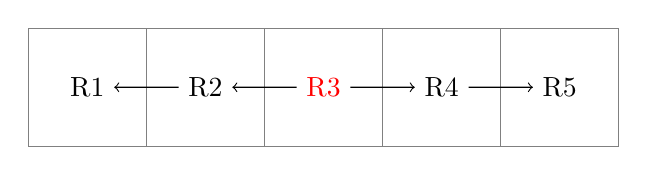
\begin{tikzpicture}[scale = 1.5]
\draw[color = gray] (0,0) grid[xstep = 1cm, ystep = 1cm] (5,1);
\node (R1) at (.5, .5) {R1};
\node (R2) at (1.5,.5) {R2};
\node (R3) [color =  red]  at (2.5,.5) {R3};
\node (R4) at (3.5,.5) {R4};
\node (R5) at (4.5,.5) {R5};
\draw [->] (R3) -- (R2);
\draw [->] (R3) -- (R4);
\draw [->] (R2) -- (R1);
\draw [->] (R4) -- (R5);
\end{tikzpicture}
\end{figure}
%-------------------------------------------

Similarly, when studying crime at the city level, it is crucial to incorporate the possibility that crime is localized. The identification of concentrations or clusters of higher criminal activity has become a central mechanism for targeting criminal justice and crime prevention responses. These crime clusters, commonly referred to as \textbf{hotspots}, represent geographic locations with high crime concentrations relative to the overall distribution of crime across the entire region of interest.

Both examples implicitly highlight the significance of geographic location and distance. They underscore the importance of the first law of geography, as articulated by Waldo Tobler: \emph{``everything is related to everything else, but near things are more related than distant things''}. This foundational principle gives rise to fundamental concepts such as \textbf{spatial dependence} and \textbf{spatial autocorrelation}.\index{Tobler's law}

%---------------------------------------------
\subsection{Spatial Dependence}\label{sec:spatial_dependence}\index{Spatial dependence}
%---------------------------------------------

Spatial dependence occurs when the values observed at one location or region, say observation $i$, depend on the values of neighboring observations at nearby locations. Formally, we can express this as:
\begin{equation*}
  y_i = f(y_j),\quad i = 1,\ldots,n\;, j\neq i.
\end{equation*}

In simpler terms, what happens in region $i$ depends on what happens in region $j$ for all $j \neq i$. For example, using our previous example displayed in Figure \ref{fig:example_poll}, we would like to estimate 
\begin{equation*}
  \begin{aligned}
y_1 & = \beta_{21} y_2 + \beta_{31} y_3 + \beta_{41} y_4 + \beta_{51} y_5 + \epsilon_1, \\
y_2 & = \beta_{12} y_1 + \beta_{32} y_3 + \beta_{42} y_4 + \beta_{52} y_5 + \epsilon_2, \\
y_3 & = \beta_{13} y_1 + \beta_{23} y_2 + \beta_{43} y_4 + \beta_{53} y_5 + \epsilon_3, \\
y_4 & = \beta_{14} y_1 + \beta_{24} y_2 + \beta_{34} y_3 + \beta_{54} y_5 + \epsilon_4, \\
y_5 & = \beta_{15} y_1 + \beta_{25} y_2 + \beta_{35} y_3 + \beta_{45} y_5 + \epsilon_5, 
\end{aligned}
\end{equation*}
%
where $\beta_{ji}$ represents the effect of pollution in region $j$ on region $i$. However, this model becomes impractical as it would result in a system with many more parameters than observations. With $n = 5$ observations, we would have to estimate 20 parameters, exceeding the available degrees of freedom. Intuitively, allowing for dependence relations between a set of $n$ observations/locations introduces potentially $n^2 - n$ relations, accounting for the exclusion of dependence on oneself.

The crucial point is that, under standard econometric modeling, incorporating spatial dependency in such a manner is impractical. However, as we will explore in the next sections, we can efficiently integrate spatial relationships using the so-called \textbf{spatial weight matrix}. 

%===========================================
\subsection{Spatial Autocorrelation}\label{sec:Spatial_autocorrelation}
%===========================================

Another crucial concept is \textbf{spatial autocorrelation}\index{Spatial autocorrelation}. In a spatial context, autocorrelation denotes the correlation between the values of a variable at two different locations. It can also be defined as the correlation between the same attribute at two (or more) different locations or the coincidence of values' similarity with location similarity. Essentially, spatial autocorrelation investigates whether the presence of a variable in one region of a spatial system makes the presence of that variable in neighboring regions more or less likely.

The counterpart of spatial autocorrelation (and spatial dependency) is spatial randomness. Spatial randomness implies the absence of any discernible spatial pattern in the data. In other words, the value observed in one spatial unit is equally likely as in any other spatial unit. Spatial randomness is important because it will form the null hypothesis later. If rejected, there is evidence of spatial structure.

As an illustrative example, Figure \ref{fig:MR} depicts the spatial distribution of poverty in the communes of the Metropolitan Region, Chile. It reveals a discernible spatial pattern where communes with similar poverty rates are clustered.
\begin{figure}[ht]
  \caption{Spatial Distribution of Poverty in Metropolitan Region, Chile}
    \label{fig:MR}
    \centering
    	\begin{minipage}{.9\linewidth}
\begin{knitrout}
\definecolor{shadecolor}{rgb}{0.969, 0.969, 0.969}\color{fgcolor}

{\centering \includegraphics[width=8cm,height=8cm]{figure/MetroRegion-1} 

}


\end{knitrout}
\footnotesize
		\emph{Notes:} This graph shows the spatial distribution of poverty in the Metropolitan Region, Chile. 
	\end{minipage}	
\end{figure}

Formally, the presence of spatial autocorrelation can be expressed through the following moment conditions:
\begin{equation*}
  \cov(y_i, y_j) = \E(y_iy_j) - \E(y_i)\E(y_j) \neq 0 \;\; \text{for} \;\; i \neq j,
\end{equation*}
%
where $y_i$ and $y_j$ are observations on a random variable at locations $i$ and $j$ in space. Here, $i$ and $j$ can represent either points or areal units. Therefore, nonzero spatial autocorrelation exists between attributes of a feature defined at locations $i$ and $j$ if the covariance between feature attribute values at those points is nonzero. If this covariance is \textbf{positive} (i.e., if data with attribute values above the mean tend to be near other data with values above the mean), then we refer to it as \textbf{positive spatial autocorrelation}; conversely, if the opposite is true, we term it \textbf{negative spatial autocorrelation}. Figure \ref{fig:Autocorrelation} illustrates examples of positive and negative spatial autocorrelation.

\begin{figure}[ht]
  \caption{Spatial Autocorrelation}
    \label{fig:Autocorrelation}
    \centering
    	\begin{minipage}{1\linewidth}
\begin{knitrout}
\definecolor{shadecolor}{rgb}{0.969, 0.969, 0.969}\color{fgcolor}

{\centering \includegraphics[width=10cm,height=10cm]{figure/Autocorrelation-1} 

}


\end{knitrout}
\footnotesize
		\emph{Notes:} Spatial Autocorrelation among 400 spatial units arranged in an 20-by-20 regular square lattice grid. Different gray-tones refer to different values of the variable ranging from low values (white) to high values (black). The left plot shows positive spatial autocorrelation, whereas right plot shows negative spatial autocorrelation. 
	\end{minipage}	
\end{figure}

Positive autocorrelation is more commonly observed, but negative autocorrelation does exist. Instances of negative autocorrelation can be found in studies on welfare competition or federal grants competitions among local governments \citep{saavedra2000model, boarnet2002federal}, regional employment \citep{filiztekin2009regional, pavlyuk2011spatial}, cross-border lottery shopping \citep{garrett2002revenue}, foreign direct investment in OECD countries \citep{garretsen2009fdi}, and the locations of the Turkish manufacturing industry \citep{basdas2009spatial}. In essence, our interest lies in studying non-random spatial patterns and explaining this non-randomness. Potential causes of non-randomness, as outlined by \cite{gibbons2015spatial}, include:

\begin{enumerate}
    \item Economic agents may be randomly allocated across space, but some characteristics of locations vary across space and influence outcomes.
    \item Location may have no causal effect on outcomes, but outcomes may be correlated across space because heterogeneous individuals or firms are non-randomly allocated across space.
    \item Individuals or firms may be randomly allocated across space, but they interact in a way that decisions by one agent affect the outcomes of other agents.
    \item Individuals or firms may be non-randomly allocated across space, and the characteristics of others nearby directly influence individual outcomes.
\end{enumerate}

%********************************
\section{Spatial Weight Matrix}\index{Weight matrix}
%********************************

One of the crucial issues in spatial econometric is the problem of formally incorporating spatial dependence into the model. As we reviewed in Section~\ref{sec:spatial_dependence}, the main problem is that we have more parameter than observations. So, the question is: What would be a good criteria to define closeness in space? Or, in other words, how to determine which other units in the system influence the one under consideration?

The device typically used in spatial analysis to define the concept of closeness in space is the so-called ``spatial weight matrix'', or more simply, $\mW$ matrix. Assuming there are $n$ spatial objects (regions, cities, countries), the $\mW$ matrix is a square matrix of dimension $n \times n$. This matrix imposes a structure in terms of identifying neighbors for each location, assigning weights that measure the intensity of the relationship among pairs of spatial units. Each element $(i,j)$ of $\mW$, denoted as $w_{ij}$, expresses the degree of spatial proximity between the pair. The matrix can be represented as follows:
\begin{equation*}
\mW = \begin{pmatrix}
        w_{11} & w_{12} & \hdots & w_{1n} \\ 
        w_{21} & w_{22} & \hdots & w_{2n} \\
        \vdots & \vdots & \ddots & \vdots \\
        w_{n1} & w_{n2} & \hdots & w_{nn} 
      \end{pmatrix}.
\end{equation*}

Generally, we assume that the diagonal elements of this ``spatial neighbors'' matrix are set to zero, indicating that ``regions are not neighbors to themselves''.

A more formal definition of a spatial weight matrix is as follows:

%-----------------------------------------------------------------------------------
\begin{definition}[Spatial Weight Matrix]\index{Weight matrix!Definition}\label{def:W}
  Let $n$ be the number of spatial units. The spatial weight matrix, $\mW$, is a $n\times n$ \textbf{positive} and \textbf{non-stochastic} matrix with element $w_{ij}$ at location $i,j$. The values of $w_{ij}$ or the weights for each pair of locations are assigned by some preset rules which define the spatial relations among locations. By convention, $w_{ij} = 0$ for the diagonal elements.
\end{definition}
%-----------------------------------------------------------------------------------

Positive means that $w_{ij}\geq 0$ for all $i\neq j$. Thus, the interactions between spatial units cannot be negative. Non-stochastic means that the researcher takes $\mW$ as known \emph{a priori}, and therefore, all results are conditional upon the specification of $\mW$.

The definition of $\mW$ also requires a rule for $w_{ij}$. In other words, we need to figure out how to assign a real number to $w_{ij}$, for $i\neq j$, representing the strength of the spatial relationship between $i$ and $j$. There are several ways of doing that. But, in general, there are two basic criteria. The first type establishes a relationship based on shared borders or vertices of lattice or irregular polygon data (contiguity). The second type establishes a relationship based on the distance between locations. Generally speaking, contiguity is most appropriate for geographic data expressed as polygons (so-called areal units), whereas distance is suited for point data, although in practice, the distinction is not that absolute. 

%==========================================
\subsection{Weights Based on Boundaries}
%==========================================

Polygon or lattice data allow for the construction of contiguity-based spatial weight matrices, which represent spatial relationships among regions. A typical specification of the contiguity relationship in such matrices is given by:
\begin{equation*}
  w_{ij}= 
   \begin{cases}
      1 & \mbox{if $i$ and $j$ are contiguous,} \\ 
      0 & \mbox{if $i$ and $j$ are not contiguous.} 
   \end{cases}
\end{equation*}

In regular grids, the definition of contiguity can vary. Drawing an analogy to chess, three common contiguity criteria are rook contiguity, bishop contiguity, and queen contiguity. Each criterion defines neighborhood relationships differently, as detailed below.

\subsubsection{Rook Contiguity}\index{Weight matrix!Rook contiguity}

Rook contiguity considers two regions as neighbors if they share a common border or side. For example, in the regular grid shown in Figure~\ref{fig:Rook_cont_grid}, which contains 9 regions (each represented as a square), the neighbors of region 5 under the rook criterion are regions 2, 4, 6, and 8 (highlighted in red).

\begin{figure}[h]
\caption{Rook Contiguity}
\label{fig:Rook_cont_grid}
\centering
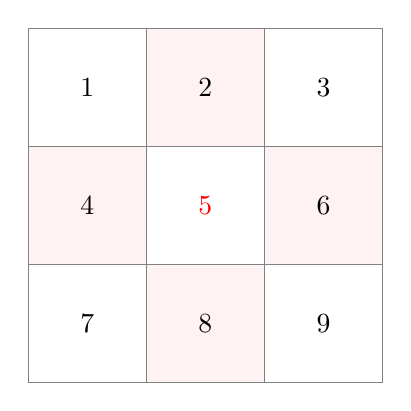
\begin{tikzpicture}[scale = 1.5]
\path [fill=red!5] (1,2) -- (2,2) -- (2,3) -- (1,3);
\path [fill=red!5] (1,0) -- (2,0) -- (2,1) -- (1,1);
\path [fill=red!5] (0,1) -- (1,1) -- (1,2) -- (0,2);
\path [fill=red!5] (2,1) -- (3,1) -- (3,2) -- (2,2);
\draw[color = gray] (0,0) grid[xstep = 1cm, ystep = 1cm] (3,3); % grid of 3 times 3
\node at (.5, 2.5) {1};
\node at (1.5, 2.5) {2};
\node at (2.5, 2.5) {3};
\node at (.5, 1.5) {4};
\node [color =  red] at (1.5,1.5) {5} ;
\node at (2.5,1.5) {6};
\node at (.5, .5) {7};
\node at (1.5,.5) {8};
\node at (2.5,.5) {9};
\end{tikzpicture}
\end{figure}

Using this criterion, the $9 \times 9$ spatial weight matrix $\mW$ is:
\begin{equation*}
  \mW = 
  \begin{pmatrix}
     0 & 1 & 0 & 1 & 0 & 0 & 0 & 0 & 0 \\
     1 & 0 & 1 & 0 & 1 & 0 & 0 & 0 & 0 \\
     0 & 1 & 0 & 0 & 0 & 1 & 0 & 0 & 0 \\
     1 & 0 & 0 & 0 & 1 & 0 & 1 & 0 & 0 \\
     0 & 1 & 0 & 1 & 0 & 1 & 0 & 1 & 0 \\
     0 & 0 & 1 & 0 & 1 & 0 & 0 & 0 & 1 \\
     0 & 0 & 0 & 1 & 0 & 0 & 0 & 1 & 0 \\
     0 & 0 & 0 & 0 & 1 & 0 & 1 & 0 & 1 \\
     0 & 0 & 0 & 0 & 0 & 1 & 0 & 1 & 0 \\
  \end{pmatrix}
\end{equation*}

\subsubsection{Bishop Contiguity}\index{Weight matrix!Bishop contiguity}

Under bishop contiguity, two regions are neighbors if they share a common corner. This criterion is less frequently used in practice. In Figure~\ref{fig:Bishop_cont_grid}, the neighbors of region 5 are regions 1, 3, 7, and 9 (highlighted in red). Note that regions located at the grid's interior have more neighbors than those along the periphery.

\begin{figure}[h]
\caption{Bishop Contiguity}
\label{fig:Bishop_cont_grid}
\centering
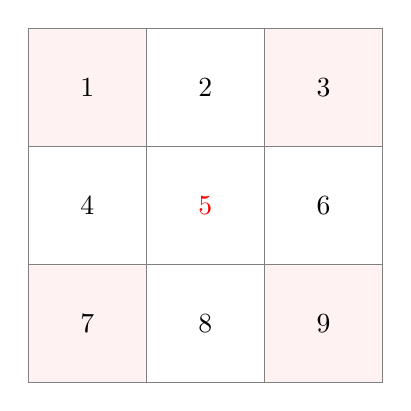
\begin{tikzpicture}[scale = 1.5]
\path [fill=red!5] (0,2) -- (1,2) -- (1,3) -- (0,3);
\path [fill=red!5] (0,0) -- (1,0) -- (1,1) -- (0,1);
\path [fill=red!5] (2,2) -- (3,2) -- (3,3) -- (2,3);
\path [fill=red!5] (2,0) -- (3,0) -- (3,1) -- (2,1);
\draw[color = gray] (0,0) grid[xstep = 1cm, ystep = 1cm] (3,3); % grid of 3 times 3
\node at (.5, 2.5) {1};
\node at (1.5, 2.5) {2};
\node at (2.5, 2.5) {3};
\node at (.5, 1.5) {4};
\node [color =  red] at (1.5,1.5) {5} ;
\node at (2.5,1.5) {6};
\node at (.5, .5) {7};
\node at (1.5,.5) {8};
\node at (2.5,.5) {9};
\end{tikzpicture}
\end{figure}

The corresponding $\mW$ matrix is:
\begin{equation*}
\mW = 
  \begin{pmatrix}
     0 & 0 & 0 & 0 & 1 & 0 & 0 & 0 & 0 \\
     0 & 0 & 0 & 1 & 0 & 1 & 0 & 0 & 0 \\
     0 & 0 & 0 & 0 & 1 & 0 & 0 & 0 & 0 \\
     0 & 1 & 0 & 0 & 0 & 0 & 0 & 1 & 0 \\
     1 & 0 & 1 & 0 & 0 & 0 & 1 & 0 & 1 \\
     0 & 1 & 0 & 0 & 0 & 0 & 0 & 1 & 0 \\
     0 & 0 & 0 & 0 & 1 & 0 & 0 & 0 & 0 \\
     0 & 0 & 0 & 1 & 0 & 1 & 0 & 0 & 0 \\
     0 & 0 & 0 & 0 & 1 & 0 & 0 & 0 & 0 \\
  \end{pmatrix}
\end{equation*}


\subsubsection{Queen Contiguity}\index{Weight matrix!Queen contiguity}

Queen contiguity considers two regions as neighbors if they share either a common side or a common corner. In Figure~\ref{fig:Queen_cont_grid}, the neighbors of region 5 include all surrounding regions: 1, 2, 3, 4, 6, 7, 8, and 9 (highlighted in red).

\begin{figure}[h]
\caption{Queen Contiguity}
\label{fig:Queen_cont_grid}
\centering
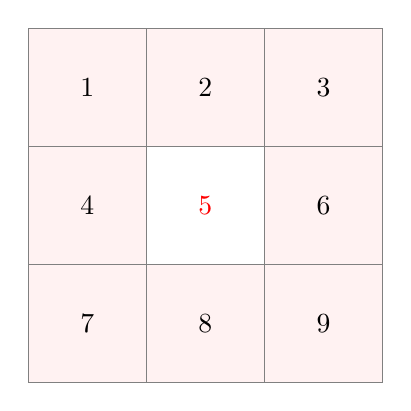
\begin{tikzpicture}[scale = 1.5]
\path [fill=red!5] (0,2) -- (1,2) -- (1,3) -- (0,3);
\path [fill=red!5] (0,0) -- (1,0) -- (1,1) -- (0,1);
\path [fill=red!5] (2,2) -- (3,2) -- (3,3) -- (2,3);
\path [fill=red!5] (2,0) -- (3,0) -- (3,1) -- (2,1);
\path [fill=red!5] (1,2) -- (2,2) -- (2,3) -- (1,3);
\path [fill=red!5] (1,0) -- (2,0) -- (2,1) -- (1,1);
\path [fill=red!5] (0,1) -- (1,1) -- (1,2) -- (0,2);
\path [fill=red!5] (2,1) -- (3,1) -- (3,2) -- (2,2);
\draw[color = gray] (0,0) grid[xstep = 1cm, ystep = 1cm] (3,3); % grid of 3 times 3
\node at (.5, 2.5) {1};
\node at (1.5, 2.5) {2};
\node at (2.5, 2.5) {3};
\node at (.5, 1.5) {4};
\node [color =  red] at (1.5,1.5) {5} ;
\node at (2.5,1.5) {6};
\node at (.5, .5) {7};
\node at (1.5,.5) {8};
\node at (2.5,.5) {9};
\end{tikzpicture}
\end{figure}


%=========================================
\subsection{Weights Based on Distance}\index{Weight matrix!Based on distance}
%=========================================

Weights can also be defined as a function of the distance between regions $i$ and $j$, denoted as $d_{ij}$. Typically, this distance is computed as the separation between centroids, although other significant points, such as capital cities or major urban centers, could also be used. Notably, unlike contiguity-based weights, distance-based matrices only require the coordinates of the relevant points.

Several methods exist to compute the distance between two spatial units. Let $x_i$ and $x_j$ represent the longitudes, and $y_i$ and $y_j$ denote the latitudes of regions $i$ and $j$. The \textbf{Minkowski}\index{Weight matrix!Minkowki} metric provides a general formula for distance:
\begin{equation*}
  d_{ij}^p = \left(\left|x_i - x_j\right|^p + \left|y_i - y_j\right|^p\right),
\end{equation*}
%
where $p$ is a parameter that allows flexibility in distance computation. A commonly used variant is the Euclidean distance, which corresponds to $p = 2$:
\begin{equation*}
  d_{ij}^e = \sqrt{(x_i - x_j)^2 + (y_i - y_j)^2}.
\end{equation*}

Another popular alternative is the Manhattan (or block) distance, which considers movement along east-west and north-south directions, i.e., along straight angles. This metric corresponds to $p = 1$:
\begin{equation*}
   d_{ij}^m = \left|x_i - x_j\right| + \left|y_i - y_j\right|.
\end{equation*}

While these metrics are suitable for treating the Earth as a plane, they may lack accuracy over larger distances due to the Earth's curvature. The Euclidean distance, for instance, represents the straight-line length on a map but might not align with the shortest path on the Earth's surface. For more accurate analyses, particularly for long-distance travel, the \textbf{great circle distance} is often preferred. This method considers the Earth's curvature and calculates the shortest path between two points on a sphere. The great circle distance is given by:
\begin{equation*}
d_{ij}^{cd} = r \times \arccos^{-1}\left[\cos|x_i - x_j| \cos y_i \cos y_j + \sin y_i \sin y_j \right],
\end{equation*}
%
where $r$ is the Earth's radius. The arc distance is obtained in miles with $r = 3959$ and in kilometers with $r = 6371$.

%=================================
\subsubsection{Inverse Distance}\label{sec:inverse_distance}
%=================================

Now, we must translate information about distances among spatial points into a weight scheme. The objective is to ensure that $w_{ij} \to 0$ as $d_{ij} \to \infty$. In simpler terms, as point $j$ gets farther from point $i$, the spatial weight $w_{ij}$ should decrease, aligning with Tobler's first law.

In the inverse distance weighting scheme, the weights are inversely proportional to the separation distance, as expressed by the following formula:
\begin{equation*}
  w_{ij} =
  \begin{cases}
  \frac{1}{d_{ij}^{\alpha}} & \mbox{if} \;\;i \neq j, \\
  0 & \mbox{if}\;\; i = j,
  \end{cases}
\end{equation*}
%
where the exponent $\alpha$ is a parameter that is usually set by the researcher. In practice, the parameters are seldom estimated, but typically set to $\alpha = 1$ or $\alpha = 2$. Consequently, the weights become the reciprocal of the distance: the greater the distance between spatial units, the smaller the spatial weight or connection. Conventionally, diagonal elements of spatial weights are set to zero to avoid division by zero in the case of inverse distance weights. Plugging in a value of $d_{ii} = 0$ would yield division by zero for inverse distance weights. 

\subsubsection{Negative Exponential Model}

In the negative exponential model, weights decrease exponentially with separation distance:
\begin{equation*}
  w_{ij} = \exp\left(-\frac{d_{ij}}{\alpha}\right),
\end{equation*}
%
where $\alpha$ is again a parameter that is commonly chosen by researcher. Since the weights are given by the exponential of the negative distance, the greater the distance between $i$ and $j$, the lower $w_{ij}$.

Both the inverse distance and negative exponential distance models rely on the parameter value, functional form, and the chosen distance metric. As the weights are inversely related to distance, larger distances yield smaller weights, and vice versa. A potential challenge arises when distances are so vast that inverse distance weights approach zero, possibly resulting in a spatial weight matrix with zero values. Additionally, issues may occur if the distance metric yields values less than one, which is typically undesirable \citep{anselin2014modern}. 

\subsubsection{$k$-nearest Neighbors}

An alternative approach to spatial weights that mitigates the issue of isolates involves selecting the $k$-nearest neighbors. Unlike the distance band, this relation is not symmetric. However, a challenge arises when ties occur—when multiple locations $j$ share the same distance from $i$. Several solutions exist to address ties, ranging from randomly selecting one of the $k$-th order neighbors to including all of them.

\subsubsection{Threshold Distance (Distance Band Weights)}

In contrast to the $k$-nearest neighbors method, the threshold distance specifies that a region $i$ is neighbor of $j$ if the distance between them is less than a specified maximum distance:
\begin{equation*}
  w_{ij}= 
   \begin{cases}
      1 & \mbox{if}\;\; 0\leq d_{ij} \leq d_{max}, \\ 
      0 & \mbox{if}\;\; d_{ij} > d_{max}.
   \end{cases}
\end{equation*}


To prevent isolates resulting from an excessively stringent critical distance, the distance must be chosen so that each location has at least one neighbor. Such a distance conforms to a max-min criterion, i.e., it is the largest of the nearest neighbor distances.

Importantly, a weights matrix derived from a distance band is always symmetric, as distance is inherently a symmetric relation.

%============================================
\subsection{Row-Standardized Weights Matrix}\index{Weight matrix!Row-standardization}
%============================================

In practical applications, spatial weights are rarely used in their raw binary (or distance) form. Instead, they are often transformed or standardized to improve interpretability and comparability. One common approach is to compute weighted averages, placing greater emphasis on nearby observations than on distant ones. To achieve this, a \textbf{row-standardized} weight matrix $\mW^s$ is defined, with elements $w_{ij}^s$ given by:
\begin{equation*}
w_{ij}^s = \frac{w_{ij}}{\sum_{j = 1}^n w_{ij}}.
\end{equation*}

This formulation ensures that all weights lie within the range of 0 to 1, facilitating the interpretation of matrix operations as an averaging of neighboring values. Moreover, row-standardization enhances the comparability of spatial parameters across models in various spatial stochastic processes \citep{AnselinBera1998}.

An additional feature of row-standardized matrices is that the sum of the weights in each row equals unity, and the total sum of all weights, $S_0 = \sum_i\sum_j w_{ij}$, equals the number of observations, $n$. This property simplifies the interpretation and application of the weights, as we will explore further in subsequent sections.

However, a key consequence of row-standardization is the loss of symmetry in the spatial weights matrix. While symmetric matrices have the desirable property of real eigenvalues, row-standardized matrices are generally asymmetric and do not preserve this characteristic. Nevertheless, row-standardization remains prevalent in applied work due to its intuitive interpretation and computational convenience.

Row-standardized matrices are also referred to as row-stochastic or Markov matrices. Formally, a row-stochastic matrix is defined as follows:
%%%%%%%%%%%%%%%%%%%%%%%%%%%%%%%%%%%%%%%%%%
\begin{definition}[Row-stochastic Matrix]
	A real $n\times n$ matrix $\mA$ is called \textbf{Markov} matrix or \textbf{row-stochastic matrix} if 
		\begin{enumerate}
			\item $a_{ij} \geq 0$ for $1\leq i, j \leq n$;
			\item $\sum_{j=1}^n a_{ij} = 1$ for $1\leq i \leq n$
		\end{enumerate}
\end{definition}
%%%%%%%%%%%%%%%%%%%%%%%%%%%%%%%%%%%%%%%%%%

An important property of row-stochastic matrices concerns their eigenvalues:

%%%%%%%%%%%%%%%%%%%%%%%%%%%%%%%%%%%%%%%%%%%
\begin{theorem}[Eigenvalues of row-stochastic Matrix]\label{teo:eigen_values}
	Every eigenvalue $\omega_i$ of a row-stochastic Matrix satisfies $\left|\vomega\right|\leq 1$
\end{theorem}
%%%%%%%%%%%%%%%%%%%%%%%%%%%%%%%%%%%%%%%%%%%

Therefore, the eigenvalues of the row-stochastic (i.e., row-normalized, row standardized or Markov) neighborhood matrix $\mW^s=(w_{ij}^s)$ are in the range $\left[-1, +1\right]$.

Finally, the behavior of $\mW^s$ is important for asymptotic properties of estimators and test statistics \citep[][pp. 244]{AnselinBera1998}. In particular, the $\mW$ matrix should be also exogenous, unless endogeneity is considered explicitly in the model specification. 

%============================================
\subsection{Spatial Lagged Variables}\label{sec:spatial_lag_var}\index{Weight matrix!Spatial lag}
%============================================

Having explored the spatial weight matrix, we can now introduce the concept of  \textbf{spatially lagged variables} or \textbf{spatial lag operator}. The spatial lag operator takes the form $\vy_L = \mW\vy$ with dimension $n \times 1$, where each element is given by $\vy_{Li} = \sum_{j = 1}^nw_{ij}y_j$, i.e., a weighted average of the $\vy$ values in the neighbor of $i$.

For example, consider 
\begin{equation*}
  \mW\vy =    \begin{pmatrix}
     0 & 1 & 0 \\
     1 & 0 & 1 \\
     0 & 1 & 0
  \end{pmatrix}
  \begin{pmatrix}
     10 \\
     50 \\
     30
  \end{pmatrix} =
  \begin{pmatrix}
     50 \\
     10 + 30 \\
     50
  \end{pmatrix}.
\end{equation*}

Using a row-standardized weight matrix:
\begin{equation*}
  \mW^s\vy =    \begin{pmatrix}
     0 & 1 & 0 \\
     0.5 & 0 & 0.5 \\
     0 & 1 & 0
  \end{pmatrix}
  \begin{pmatrix}
     10 \\
     50 \\
     30
  \end{pmatrix} =
  \begin{pmatrix}
     50 \\
     5 + 15 \\
     50
  \end{pmatrix}.
\end{equation*}

Consequently, for spatial unit $i$, the spatial lag of $y_i$, denoted a $\vy_{Li}$ (the variable $\mW\vy$ observed for location $i$) is:
\begin{equation*}
  \vy_{Li} = w_{i, 1}^sy_i + w_{i, 2}^sy_2 + \cdots + w_{i, n}^sy_n, 
\end{equation*}
%
or equivalently,
\begin{equation*}
  \vy_{Li} = \sum_{j = 1}^nw_{i,j}^sy_j,
\end{equation*}
%
where the weights $w_{ij}$ are the elements of the $i$th row of the matrix $\mW^s$ matched with the corresponding elements of the vector $\vy$. In other words, this represents a weighted sum of values observed at neighboring locations, excluding non-neighbors.

\begin{remark}
As stated by \citet[][p. 23-24]{anselin1988spatial}, standardization must be done with caution.\footnote{See also \citet[][p. 12]{elhorst2014spatial} and references therein.} For example, when the weights are based on an inverse distance function (or similar concept of distance decay), which has a meaningful economic interpretation, scaling the rows so that the weights sum to one may result in a loss of that interpretation. Can you give an example?
\end{remark}


%============================================
\subsection{Higher Order Spatial Weights}\label{sec:HSO}\index{Weight matrix!Higher order}
%============================================

To expand our understanding of geographical space as defined by the matrix $\mW$, we turn to the concept of higher-order neighbors. These are neighbors that are not directly adjacent but are reachable through other spatial units. For instance, we might consider the neighbors of a spatial unit's neighbors or even their neighbors' neighbors. To formalize this, we introduce the notion of \textbf{higher-order spatial weight matrices}.

The higher-order spatial weight matrix of order $l$, denoted as $\mW^l$, is defined as:
\begin{equation*}
  \mW^l = \underbrace{\mW \mW \cdots \mW}_{l \text{ times}}.
\end{equation*}

For example:
\begin{itemize}
\item The second-order spatial weight matrix is $\mW^2 = \mW\mW$.
\item The third-order spatial weight matrix is $\mW^3 = \mW \mW\mW$, and so on.
\end{itemize}

The element $w_{ij}$ in these higher-order matrices represents whether spatial unit $j$ is a neighbor of order $l$ to spatial unit $i$. Specifically:
\begin{itemize}
\item For $l = 2$, $w_{ij}$ equals 1 if $j$ is adjacent to a first-order neighbor of $i$, and 0 otherwise.
\item For $l = n$, $w_{ij}$ equals 1 if $j$ is adjacent to the $(n-1)$-order neighbors of $i$, and 0 otherwise.
\end{itemize}

To illustrate these points, consider the following spatial structure from example in Section \ref{sec:why_se}:
\begin{equation}\label{eq:W5x5}
\mW = \begin{pmatrix}
      0 & 1 & 0 & 0 & 0 \\
      1 & 0 & 1 & 0 & 0 \\
      0 & 1 & 0 & 1 & 0 \\
      0 & 0 & 1 & 0 & 1 \\
      0 & 0 & 0 & 1 & 0
      \end{pmatrix}.
\end{equation}

Then, $\mW^2 = \mW\mW$ based on the $5\times 5$ first-order contiguity matrix $\mW$ from \eqref{eq:W5x5} is:
\begin{equation}
\mW^2 = \begin{pmatrix}\label{eq:W25x5}
      1 & 0 & 1 & 0 & 0 \\
      0 & 2 & 0 & 1 & 0 \\
      1 & 0 & 2 & 0 & 1 \\
      0 & 1 & 0 & 2 & 0 \\
      0 & 0 & 1 & 0 & 1
      \end{pmatrix}
\end{equation}

For region $R1$, the second-order neighbors are $R1$ and $R3$. This indicates that $R1$ is its own second-order neighbor (via feedback) and also shares second-order adjacency with $R3$, which is a first-order neighbor of $R2$. 

Now consider R2. The first panel of Figure \ref{fig:example_hon} shows the first-order neighbors of $R2$ based on the spatial weight matrix in \eqref{eq:W5x5}: $R1$ and $R3$. Panel B considers the second-order neighbors of $R2$: $R2$ itself and $R4$. To understand this, note that there is a feedback effect from the first impact from $R2$ coming from $R1$ and $R3$ (first-order neighbors of $R2$). This explains why the element $w^2_{22} = 2$. Additionally, there is an indirect effect coming from $R4$ through $R3$ that finally impacts $R2$, yielding a value of 1 for the element $w^2_{24}$.

Similarly, for region $R3$, the second-order neighbors are regions $R1$ (which is a neighbor to the neighboring region $R2$), $R3$ (a second-order neighbor to itself), and $R5$ (which is a neighbor to the neighboring region $R4$). 

\begin{figure}[ht]
\caption{Higher-Order Neighbors}
\label{fig:example_hon}
\centering
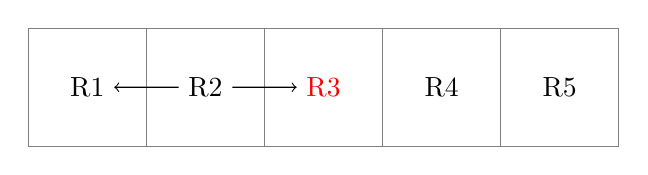
\begin{tikzpicture}[scale = 1.5]
\draw[color = gray] (0,0) grid[xstep = 1cm, ystep = 1cm] (5,1);
\node (R1) at (.5, .5) {R1};
\node (R2) at (1.5,.5) {R2};
\node (R3) [color =  red]  at (2.5,.5) {R3};
\node (R4) at (3.5,.5) {R4};
\node (R5) at (4.5,.5) {R5};
\draw [->] (R2) -- (R1);
\draw [->] (R2) -- (R3);
\end{tikzpicture}
\\
\vspace{1cm}
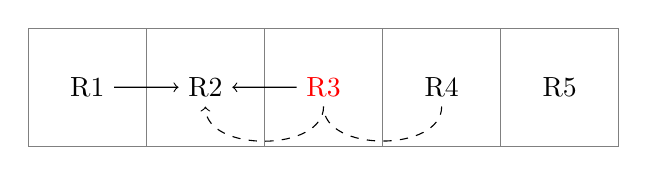
\begin{tikzpicture}[scale = 1.5]
\draw[color = gray] (0,0) grid[xstep = 1cm, ystep = 1cm] (5,1);
\node (R1) at (.5, .5) {R1};
\node (R2) at (1.5,.5) {R2};
\node (R3) [color =  red]  at (2.5,.5) {R3};
\node (R4) at (3.5,.5) {R4};
\node (R5) at (4.5,.5) {R5};
\draw [->] (R1) -- (R2);
\draw [->] (R3) -- (R2);
\draw [->, dashed] (R4) to[out= 270,in=270] (R3) to[out=270,in=270] (R2);
\end{tikzpicture}
\end{figure}

Similarly, the third-order neighbors are: 
\begin{equation*}
\mW^3 = \begin{pmatrix}
      0 & 2 & 0 & 1 & 0 \\
      2 & 0 & 3 & 0 & 1 \\
      0 & 3 & 0 & 3 & 0 \\
      1 & 0 & 3 & 0 & 2 \\
      0 & 1 & 0 & 2 & 1
      \end{pmatrix}
\end{equation*}

Could you explain the elements of this matrix?

%============================================
\section{Examples of Weight Matrices in R}
%============================================

Creating spatial weight matrices manually is a tedious and error-prone process, especially for large datasets. Fortunately, modern statistical software provides robust tools to simplify this task. To start, we typically need a \textbf{shapefile}, a widely used format for storing geographical information.

The shapefile format is a digital vector storage format that supports geometric data types such as points, lines, and polygons, along with associated attributes. It enables diverse representations of geographic data by combining shapes with their corresponding attribute data. A complete shapefile consists of three mandatory files with the following extensions:
\begin{itemize}
  \item \texttt{.shp}: The shape file containing the feature geometry.
  \item \texttt{.shx}: The shape index file, which facilitates fast positional indexing of the feature geometry.
  \item \texttt{.dbf}: The attribute file, formatted in \texttt{dBase} IV format, storing columnar attributes for each shape.
\end{itemize}

These three components must be present for a shapefile to be functional. The \texttt{.shp} file stores the actual geometric data, while the \texttt{.shx} and \texttt{.dbf} files provide supporting information to enable efficient access and attribute storage.

In this example, we demonstrate how to create spatial weight matrices using \proglang{R}. Specifically, we focus on a map of the communes in the Metropolitan Region of Chile. To begin, we load the shapefile into \proglang{R} using the \pkg{sf} package \citep{pabesmasf}, which is designed for handling spatial data.

\begin{knitrout}
\definecolor{shadecolor}{rgb}{0.969, 0.969, 0.969}\color{fgcolor}\begin{kframe}
\begin{alltt}
\hlcom{#Load package sf}
\hlkwd{library}\hldef{(}\hlsng{"sf"}\hldef{)}
\end{alltt}
\end{kframe}
\end{knitrout}

If the shapefile \texttt{mr\_chile.shp} is located in the working directory, we can load it using the \texttt{read\_sf} function:
\begin{knitrout}
\definecolor{shadecolor}{rgb}{0.969, 0.969, 0.969}\color{fgcolor}\begin{kframe}
\begin{alltt}
\hlcom{# Read shape file}
\hldef{mr} \hlkwb{<-} \hlkwd{read_sf}\hldef{(}\hlsng{"mr_chile.shp"}\hldef{)}
\hlkwd{class}\hldef{(mr)}
\end{alltt}
\begin{verbatim}
## [1] "sf"         "tbl_df"     "tbl"        "data.frame"
\end{verbatim}
\end{kframe}
\end{knitrout}

The \code{read\_sf} function reads data from the shapefile into an object of class ``\code{sf}''. The \code{names} function provides the name of the variables in the \texttt{.dbf} file associated with the shape file. 
\begin{knitrout}
\definecolor{shadecolor}{rgb}{0.969, 0.969, 0.969}\color{fgcolor}\begin{kframe}
\begin{alltt}
\hlcom{# Names of the variables in .dbf}
\hlkwd{names}\hldef{(mr)}
\end{alltt}
\begin{verbatim}
##  [1] "ID"         "NAME"       "NAME2"      "URB_POP"    "RUR_POP"   
##  [6] "MALE_POP"   "TOT_POP"    "FEM_POP"    "N_PARKS"    "N_PLAZA"   
## [11] "CONS_HOUSE" "M2_CONS_HA" "GREEN_AREA" "AREA"       "POVERTY"   
## [16] "PER_CONTR_" "PER_HON_SA" "PER_PLANT_" "NURSES"     "DOCTORS"   
## [21] "CONSULT_RU" "CONSULT_UR" "POSTAS"     "ESTAB_MUN_" "PSU_MUN_PR"
## [26] "PSU_PART_P" "PSU_SUB_PR" "STUDENT_SU" "STUDENT_PA" "STUDENT_MU"
## [31] "geometry"
\end{verbatim}
\end{kframe}
\end{knitrout}

Now, let's visualize the shapefile using the \code{plot} function:
\begin{knitrout}
\definecolor{shadecolor}{rgb}{0.969, 0.969, 0.969}\color{fgcolor}\begin{kframe}
\begin{alltt}
\hlcom{# Plot shapefile}
\hlkwd{plot}\hldef{(}\hlkwd{st_geometry}\hldef{(mr),} \hlkwc{main} \hldef{=} \hlsng{"Metropolitan Region-Chile"}\hldef{,} \hlkwc{axes} \hldef{=} \hlnum{TRUE}\hldef{)}
\end{alltt}
\end{kframe}
\end{knitrout}

The metropolitan region with its 52 communes is shown in Figure \ref{fig:plot_mr}.

\begin{figure}[h]
  \caption{Plotting a Map in R}
    \label{fig:plot_mr}
\begin{knitrout}
\definecolor{shadecolor}{rgb}{0.969, 0.969, 0.969}\color{fgcolor}

{\centering \includegraphics[width=9cm,height=9cm]{figure/plot_mr-1} 

}


\end{knitrout}
\end{figure}

%===============================================
\subsection{Creating Contiguity Neighbors}\label{sec:computing-W-in-R}
%===============================================

To construct spatial weight matrices, the \pkg{spdep} package \citep{bivand2013computing} provides an extensive suite of tools. After installation, the package can be loaded as follows:

\begin{knitrout}
\definecolor{shadecolor}{rgb}{0.969, 0.969, 0.969}\color{fgcolor}\begin{kframe}
\begin{alltt}
\hlcom{#Load package}
\hlkwd{library}\hldef{(}\hlsng{"spdep"}\hldef{)}
\end{alltt}
\end{kframe}
\end{knitrout}

In \pkg{spdep}, neighbor relationships between $n$ observations are represented by objects of class \texttt{nb}. These objects are lists of length $n$, where each element is an integer vector containing the indices of neighboring regions. If a region has no neighbors, the corresponding element is assigned an integer value of zero.

The \texttt{poly2nb} function constructs neighbor relationships based on \textbf{contiguity}, generating a neighbors list of class \texttt{nb}. This function supports both the Queen and Rook criteria for defining spatial relationships. Refer to \texttt{help(poly2nb)} for detailed documentation.


As explained in previous section, the Queen criterion defines neighbors as regions that share at least one vertex or edge. The following example demonstrates how to construct a neighbor list for the communes in the Metropolitan Region of Chile:\index{Weight matrix!\texttt{poly2nb} function}

\begin{knitrout}
\definecolor{shadecolor}{rgb}{0.969, 0.969, 0.969}\color{fgcolor}\begin{kframe}
\begin{alltt}
\hlcom{# Create queen W}
\hlkwd{sf_use_s2}\hldef{(}\hlnum{FALSE}\hldef{)}
\hldef{queen.w} \hlkwb{<-} \hlkwd{poly2nb}\hldef{(}\hlkwd{as}\hldef{(mr,} \hlsng{"Spatial"}\hldef{),} \hlkwc{queen} \hldef{=}  \hlnum{TRUE}\hldef{,} \hlkwc{row.names} \hldef{= mr}\hlopt{$}\hldef{NAME)}
\end{alltt}
\end{kframe}
\end{knitrout}

Once the \texttt{nb} object is created, it can be explored using standard methods such as \texttt{print}, \texttt{summary}, and \texttt{plot}. For example, the summary of the Queen-based neighbors list provides information about the spatial relationships:
\begin{knitrout}
\definecolor{shadecolor}{rgb}{0.969, 0.969, 0.969}\color{fgcolor}\begin{kframe}
\begin{alltt}
\hlcom{# Summary of W}
\hlkwd{summary}\hldef{(queen.w)}
\end{alltt}
\begin{verbatim}
## Neighbour list object:
## Number of regions: 52 
## Number of nonzero links: 292 
## Percentage nonzero weights: 10.79882 
## Average number of links: 5.615385 
## Link number distribution:
## 
##  2  3  4  5  6  7  8  9 10 12 
##  3  2  7 15 10 10  2  1  1  1 
## 3 least connected regions:
## Tiltil San Pedro Maria Pinto with 2 links
## 1 most connected region:
## San Bernardo with 12 links
\end{verbatim}
\end{kframe}
\end{knitrout}

The output provides crucial information about the neighbors, including the number of regions (52 communes in this example), the number of nonzero links, the percentage of nonzero weights, the average number of links, and more.

For instance, the commune of San Bernardo stands out as the most connected region with 12 neighbors under the queen scheme. Conversely, the least connected regions are Tiltil, San Pedro, and Maria Pinto, each with only 2 neighbors. The output also shows the distribution of neighbors, revealing that 7 out of 52 regions have 4 neighbors, and only 2 communes have 8 neighbors.

To visualize the region with the largest number of neighbors (San Bernardo) and its immediate neighbors, use the following code:
\begin{knitrout}
\definecolor{shadecolor}{rgb}{0.969, 0.969, 0.969}\color{fgcolor}\begin{kframe}
\begin{alltt}
\hlcom{# Plot communes with largest number of contiguities}
\hldef{cards} \hlkwb{<-} \hlkwd{card}\hldef{(queen.w)}
\hldef{maxconts} \hlkwb{<-} \hlkwd{which}\hldef{(cards} \hlopt{==} \hlkwd{max}\hldef{(cards))}
\hldef{fg} \hlkwb{<-} \hlkwd{rep}\hldef{(}\hlsng{"grey"}\hldef{,} \hlkwd{length}\hldef{(cards))}
\hldef{fg[maxconts]} \hlkwb{<-} \hlsng{"red"}
\hldef{fg[queen.w[[maxconts]]]} \hlkwb{<-} \hlsng{"blue"}
\hlkwd{plot}\hldef{(}\hlkwd{st_geometry}\hldef{(mr),} \hlkwc{col} \hldef{= fg)}
\end{alltt}
\end{kframe}
\end{knitrout}

\begin{figure}[ht]
  \caption{Commune with largest number of contiguities}
    \label{fig:plot_nn}
    \centering
        	\begin{minipage}{1\linewidth}
\begin{knitrout}
\definecolor{shadecolor}{rgb}{0.969, 0.969, 0.969}\color{fgcolor}

{\centering \includegraphics[width=10cm,height=10cm]{figure/neight-1} 

}


\end{knitrout}
\footnotesize
		\emph{Notes:} The commune in red is the spatial unit (San Bernardo) with the largest number of neighbors based on the queen criteria, whereas the communes in blue are its neighbors. 
	\end{minipage}	
\end{figure}

Figure \ref{fig:plot_nn} provides a visual representation where the red-colored commune, San Bernardo, stands out as the spatial unit with the largest number of neighbors according to the queen criteria. Meanwhile, the communes in blue represent its neighboring units.

To transform the \code{list} into an actual matrix $\mW$, we can use the \code{nb2listw} function\index{Weight matrix!\texttt{nb2listw} function}:

\begin{knitrout}
\definecolor{shadecolor}{rgb}{0.969, 0.969, 0.969}\color{fgcolor}\begin{kframe}
\begin{alltt}
\hlcom{# From list to matrix}
\hldef{queen.wl} \hlkwb{<-} \hlkwd{nb2listw}\hldef{(queen.w,} \hlkwc{style} \hldef{=} \hlsng{"W"}\hldef{)}
\hlkwd{summary}\hldef{(queen.wl)}
\end{alltt}
\begin{verbatim}
## Characteristics of weights list object:
## Neighbour list object:
## Number of regions: 52 
## Number of nonzero links: 292 
## Percentage nonzero weights: 10.79882 
## Average number of links: 5.615385 
## Link number distribution:
## 
##  2  3  4  5  6  7  8  9 10 12 
##  3  2  7 15 10 10  2  1  1  1 
## 3 least connected regions:
## Tiltil San Pedro Maria Pinto with 2 links
## 1 most connected region:
## San Bernardo with 12 links
## 
## Weights style: W 
## Weights constants summary:
##    n   nn S0       S1      S2
## W 52 2704 52 19.76751 216.466
\end{verbatim}
\end{kframe}
\end{knitrout}

An important argument for \code{nb2listw} is \code{style}. This argument indicates what type of matrix to create. For example, \code{style = "W"} creates a row-standardize matrix so that $w^s_{ij} = w_{ij}/ \sum_j w_{ij}$. After normalization, each row of $\mW^s$ sums to 1. Other options include \code{"B"} for basic binary coding; \code{"C"} for global standarization, that is, $w^s_{ij} = w_{ij} \cdot (n/ \sum_{i}\sum_j w_{ij})$. If \code{style = "U"}, then $w^s_{ij} = w_{ij}/ \sum_i\sum_j w_{ij}$. In a \code{minmax} matrix, the $(i,j)$th element of $\mW^s$  becomes $w^s_{ij} = w_{ij} / \min\left\lbrace \max_i(\tau_i), \max_i(c_i)\right\rbrace$, with $\max_i(\tau_i)$ being the largest row sum of $\mW$ and $\max_i(c_i)$ being the largest column sum of $\mW$ \citep{kelejian2010specification}. Finally, \code{"S"} is the variance-stabilizing coding scheme where $w^s_{ij} = w_{ij}/ \sqrt{\sum_j w_{ij} ^2}$ \citep{tiefelsdorf1999variance}. 

Additionally, the \code{summary} function provides several constants essential for global spatial autocorrelation statistics, which we will discuss later. 

We can also inspect the attributes of the object using the function \code{attributes}:

\begin{knitrout}
\definecolor{shadecolor}{rgb}{0.969, 0.969, 0.969}\color{fgcolor}\begin{kframe}
\begin{alltt}
\hlcom{# Attributes of wlist}
\hlkwd{attributes}\hldef{(queen.w)}
\end{alltt}
\begin{verbatim}
## $class
## [1] "nb"
## 
## $region.id
##  [1] "Santiago"            "Cerillos"            "Cerro Navia"        
##  [4] "Conchali"            "El Bosque"           "Estacion Central"   
##  [7] "La Cisterna"         "La Florida"          "La Granja"          
## [10] "La Pintana"          "La Reina"            "Lo Espejo"          
## [13] "Lo Prado"            "Macul"               "Nunoa"              
## [16] "Pedro Aguirre Cerda" "Penalolen"           "Providencia"        
## [19] "Quinta Normal"       "Recoleta"            "Renca"              
## [22] "San Joaquin"         "San Miguel"          "San Ramon"          
## [25] "Independencia"       "Puente Alto"         "Las Condes"         
## [28] "Vitacura"            "Quilicura"           "Huechuraba"         
## [31] "Maipu"               "Pudahuel"            "San Bernardo"       
## [34] "Tiltil"              "Lampa"               "Colina"             
## [37] "Lo Barnechea"        "Pirque"              "Paine"              
## [40] "Buin"                "Alhue"               "Melipilla"          
## [43] "San Pedro"           "Maria Pinto"         "Curacavi"           
## [46] "Penaflor"            "Calera de Tango"     "Padre Hurtado"      
## [49] "El Monte"            "Talagante"           "Isla de Maipo"      
## [52] "San Jose de Maipo"  
## 
## $call
## poly2nb(pl = as(mr, "Spatial"), row.names = mr$NAME, queen = TRUE)
## 
## $type
## [1] "queen"
## 
## $snap
## [1] 1.490116e-08
## 
## $sym
## [1] TRUE
## 
## $ncomp
## $ncomp$nc
## [1] 1
## 
## $ncomp$comp.id
##  [1] 1 1 1 1 1 1 1 1 1 1 1 1 1 1 1 1 1 1 1 1 1 1 1 1 1 1 1 1 1 1 1 1 1 1 1 1 1 1
## [39] 1 1 1 1 1 1 1 1 1 1 1 1 1 1
\end{verbatim}
\end{kframe}
\end{knitrout}

Weight matrices based on contiguity are generally symmetric. Use the following command to verify:
\begin{knitrout}
\definecolor{shadecolor}{rgb}{0.969, 0.969, 0.969}\color{fgcolor}\begin{kframe}
\begin{alltt}
\hlcom{# Symmetric W}
\hlkwd{is.symmetric.nb}\hldef{(queen.w)}
\end{alltt}
\begin{verbatim}
## [1] TRUE
\end{verbatim}
\end{kframe}
\end{knitrout}

The Rook criterion considers neighbors that share a common edge. Here's how to construct a Rook-based neighbors list:
\begin{knitrout}
\definecolor{shadecolor}{rgb}{0.969, 0.969, 0.969}\color{fgcolor}\begin{kframe}
\begin{alltt}
\hlcom{# Rook W}
\hldef{rook.w} \hlkwb{<-} \hlkwd{poly2nb}\hldef{(}\hlkwd{as}\hldef{(mr,} \hlsng{"Spatial"}\hldef{),} \hlkwc{row.names} \hldef{= mr}\hlopt{$}\hldef{NAME,} \hlkwc{queen} \hldef{=}  \hlnum{FALSE}\hldef{)}
\hlkwd{summary}\hldef{(rook.w)}
\end{alltt}
\begin{verbatim}
## Neighbour list object:
## Number of regions: 52 
## Number of nonzero links: 272 
## Percentage nonzero weights: 10.05917 
## Average number of links: 5.230769 
## Link number distribution:
## 
##  2  3  4  5  6  7  8  9 10 
##  3  3 12 16  7  6  2  1  2 
## 3 least connected regions:
## Tiltil San Pedro Maria Pinto with 2 links
## 2 most connected regions:
## Santiago San Bernardo with 10 links
\end{verbatim}
\end{kframe}
\end{knitrout}

Finally, we can visualize the spatial connectivity implied by the Queen and Rook criterion using the following set of commands (see Figure \ref{fig:Queen-Rook}). 

\begin{knitrout}
\definecolor{shadecolor}{rgb}{0.969, 0.969, 0.969}\color{fgcolor}\begin{kframe}
\begin{alltt}
\hlcom{# Plot Queen and Rook W Matrices}
\hlkwd{plot}\hldef{(}\hlkwd{st_geometry}\hldef{(mr),} \hlkwc{border} \hldef{=} \hlsng{"grey"}\hldef{)}
\hldef{coords} \hlkwb{<-} \hlkwd{st_coordinates}\hldef{(}\hlkwd{st_centroid}\hldef{(}\hlkwd{st_geometry}\hldef{(mr)))}
\hlkwd{plot}\hldef{(queen.w, coords,} \hlkwc{add} \hldef{=}  \hlnum{TRUE}\hldef{,} \hlkwc{col} \hldef{=} \hlsng{"red"}\hldef{)}
\hlkwd{plot}\hldef{(rook.w, coords,} \hlkwc{add} \hldef{=}  \hlnum{TRUE}\hldef{,} \hlkwc{col} \hldef{=} \hlsng{"yellow"}\hldef{)}
\end{alltt}
\end{kframe}
\end{knitrout}

\begin{figure}[ht]
  \caption{Queen and Rook Criteria for MR}
    \label{fig:Queen-Rook}
\begin{knitrout}
\definecolor{shadecolor}{rgb}{0.969, 0.969, 0.969}\color{fgcolor}

{\centering \includegraphics[width=8cm,height=8cm]{figure/plot-queen-rookT-1} 

}


\end{knitrout}
\end{figure}

%==================================================
\subsection{Creating Distance-based Neighbors}
%==================================================

We proceed to build spatial weight matrices using the $k$-nearest neighbors criteria\index{Weight matrix!\texttt{knearneigh} function}. 

\begin{knitrout}
\definecolor{shadecolor}{rgb}{0.969, 0.969, 0.969}\color{fgcolor}\begin{kframe}
\begin{alltt}
\hlcom{# K-neighbors}
\hlkwd{head}\hldef{(coords,} \hlnum{5}\hldef{)}                                       \hlcom{# show coordinates}
\end{alltt}
\begin{verbatim}
##              X         Y
## [1,] -70.65599 -33.45406
## [2,] -70.71742 -33.50027
## [3,] -70.74504 -33.42278
## [4,] -70.67735 -33.38372
## [5,] -70.67640 -33.56294
\end{verbatim}
\begin{alltt}
\hldef{k1neigh} \hlkwb{<-} \hlkwd{knearneigh}\hldef{(coords,} \hlkwc{k} \hldef{=} \hlnum{1}\hldef{,} \hlkwc{longlat} \hldef{=} \hlnum{TRUE}\hldef{)}  \hlcom{# 1-nearest neighbor}
\hldef{k2neigh} \hlkwb{<-} \hlkwd{knearneigh}\hldef{(coords,} \hlkwc{k} \hldef{=} \hlnum{2}\hldef{,} \hlkwc{longlat} \hldef{=} \hlnum{TRUE}\hldef{)}  \hlcom{# 2-nearest neighbor}
\end{alltt}
\end{kframe}
\end{knitrout}

Here, the \code{coords}\index{Weight matrix!\texttt{coords} function} function extracts spatial coordinates from the shapefile, while \code{knearneigh} returns a matrix containing indices of points belonging to the set of $k$-nearest neighbors for each observation. The \code{k} argument specifies the number of nearest neighbors to return. If the point coordinates are given in longitude-latitude decimal degrees, distances are measured in kilometers when \code{longlat = TRUE}. For \code{longlat = FALSE}, great-circle distances are computed. The resulting objects \code{k1neigh} and \code{k2neigh} are of class \code{knn}.

Inverse distance weight matrices can be computed as follows (see Section \ref{sec:inverse_distance}):

\begin{knitrout}
\definecolor{shadecolor}{rgb}{0.969, 0.969, 0.969}\color{fgcolor}\begin{kframe}
\begin{alltt}
\hlcom{# Inverse weight matrix}
\hldef{dist.mat} \hlkwb{<-} \hlkwd{as.matrix}\hldef{(}\hlkwd{dist}\hldef{(coords,} \hlkwc{method} \hldef{=} \hlsng{"euclidean"}\hldef{))}
\hldef{dist.mat[}\hlnum{1}\hlopt{:}\hlnum{5}\hldef{,} \hlnum{1}\hlopt{:}\hlnum{5}\hldef{]}
\end{alltt}
\begin{verbatim}
##            1          2          3          4          5
## 1 0.00000000 0.07687010 0.09438408 0.07350782 0.11078109
## 2 0.07687010 0.00000000 0.08226867 0.12324109 0.07489489
## 3 0.09438408 0.08226867 0.00000000 0.07814455 0.15606360
## 4 0.07350782 0.12324109 0.07814455 0.00000000 0.17922003
## 5 0.11078109 0.07489489 0.15606360 0.17922003 0.00000000
\end{verbatim}
\begin{alltt}
\hldef{dist.mat.inv} \hlkwb{<-} \hlnum{1} \hlopt{/} \hldef{dist.mat} \hlcom{# 1 / d_\{ij\}}
\hlkwd{diag}\hldef{(dist.mat.inv)} \hlkwb{<-} \hlnum{0}      \hlcom{# 0 in the diagonal}
\hldef{dist.mat.inv[}\hlnum{1}\hlopt{:}\hlnum{5}\hldef{,} \hlnum{1}\hlopt{:}\hlnum{5}\hldef{]}
\end{alltt}
\begin{verbatim}
##           1         2         3         4         5
## 1  0.000000 13.008960 10.595007 13.603994  9.026811
## 2 13.008960  0.000000 12.155295  8.114177 13.352046
## 3 10.595007 12.155295  0.000000 12.796797  6.407644
## 4 13.603994  8.114177 12.796797  0.000000  5.579733
## 5  9.026811 13.352046  6.407644  5.579733  0.000000
\end{verbatim}
\begin{alltt}
\hlcom{# Standardized inverse weight matrix}
\hldef{dist.mat.inve} \hlkwb{<-} \hlkwd{mat2listw}\hldef{(dist.mat.inv,} \hlkwc{style} \hldef{=} \hlsng{"W"}\hldef{,} \hlkwc{row.names} \hldef{= mr}\hlopt{$}\hldef{NAME)}
\hlkwd{summary}\hldef{(dist.mat.inve)}
\end{alltt}
\begin{verbatim}
## Characteristics of weights list object:
## Neighbour list object:
## Number of regions: 52 
## Number of nonzero links: 2652 
## Percentage nonzero weights: 98.07692 
## Average number of links: 51 
## Link number distribution:
## 
## 51 
## 52 
## 52 least connected regions:
## Santiago Cerillos Cerro Navia Conchali El Bosque Estacion Central La Cisterna La Florida La Granja La Pintana La Reina Lo Espejo Lo Prado Macul Nunoa Pedro Aguirre Cerda Penalolen Providencia Quinta Normal Recoleta Renca San Joaquin San Miguel San Ramon Independencia Puente Alto Las Condes Vitacura Quilicura Huechuraba Maipu Pudahuel San Bernardo Tiltil Lampa Colina Lo Barnechea Pirque Paine Buin Alhue Melipilla San Pedro Maria Pinto Curacavi Penaflor Calera de Tango Padre Hurtado El Monte Talagante Isla de Maipo San Jose de Maipo with 51 links
## 52 most connected regions:
## Santiago Cerillos Cerro Navia Conchali El Bosque Estacion Central La Cisterna La Florida La Granja La Pintana La Reina Lo Espejo Lo Prado Macul Nunoa Pedro Aguirre Cerda Penalolen Providencia Quinta Normal Recoleta Renca San Joaquin San Miguel San Ramon Independencia Puente Alto Las Condes Vitacura Quilicura Huechuraba Maipu Pudahuel San Bernardo Tiltil Lampa Colina Lo Barnechea Pirque Paine Buin Alhue Melipilla San Pedro Maria Pinto Curacavi Penaflor Calera de Tango Padre Hurtado El Monte Talagante Isla de Maipo San Jose de Maipo with 51 links
## 
## Weights style: W 
## Weights constants summary:
##    n   nn S0       S1       S2
## W 52 2704 52 2.902384 214.3332
\end{verbatim}
\end{kframe}
\end{knitrout}

The \code{dist} function from the \pkg{stats} package computes the distance matrix using the specified metric---Euclidean distance in this example. Other available methods include \code{maximum}, \code{manhattan}, \code{canberra}, \code{binary}, and \code{minkowski}. The \code{mat2listw} function converts a square spatial weight matrix into a list format suitable for spatial analysis. For additional details on spatial weight matrices, see \cite{stewart2010choosing}.

The following code demonstrates how to plot different weight matrices:

\begin{knitrout}
\definecolor{shadecolor}{rgb}{0.969, 0.969, 0.969}\color{fgcolor}\begin{kframe}
\begin{alltt}
\hlcom{# Plot Weights}
\hlkwd{par}\hldef{(}\hlkwc{mfrow} \hldef{=} \hlkwd{c}\hldef{(}\hlnum{2}\hldef{,} \hlnum{2}\hldef{))}
\hlkwd{plot}\hldef{(}\hlkwd{st_geometry}\hldef{(mr),} \hlkwc{border} \hldef{=} \hlsng{"grey"}\hldef{,} \hlkwc{main} \hldef{=} \hlsng{"Queen"}\hldef{)}
\hlkwd{plot}\hldef{(queen.w, coords,} \hlkwc{add} \hldef{=}  \hlnum{TRUE}\hldef{,} \hlkwc{col} \hldef{=} \hlsng{"red"}\hldef{)}
\hlkwd{plot}\hldef{(}\hlkwd{st_geometry}\hldef{(mr),} \hlkwc{border} \hldef{=} \hlsng{"grey"}\hldef{,} \hlkwc{main} \hldef{=} \hlsng{"1-Neigh"}\hldef{)}
\hlkwd{plot}\hldef{(}\hlkwd{knn2nb}\hldef{(k1neigh), coords,} \hlkwc{add} \hldef{=} \hlnum{TRUE}\hldef{,} \hlkwc{col} \hldef{=} \hlsng{"red"}\hldef{)}
\hlkwd{plot}\hldef{(}\hlkwd{st_geometry}\hldef{(mr),} \hlkwc{border} \hldef{=} \hlsng{"grey"}\hldef{,} \hlkwc{main} \hldef{=} \hlsng{"2-Neigh"}\hldef{)}
\hlkwd{plot}\hldef{(}\hlkwd{knn2nb}\hldef{(k2neigh), coords,} \hlkwc{add} \hldef{=} \hlnum{TRUE}\hldef{,} \hlkwc{col} \hldef{=} \hlsng{"red"}\hldef{)}
\hlkwd{plot}\hldef{(}\hlkwd{st_geometry}\hldef{(mr),} \hlkwc{border} \hldef{=} \hlsng{"grey"}\hldef{,} \hlkwc{main} \hldef{=} \hlsng{"Inverse Distance"}\hldef{)}
\hlkwd{plot}\hldef{(dist.mat.inve, coords,} \hlkwc{add} \hldef{=}  \hlnum{TRUE}\hldef{,} \hlkwc{col} \hldef{=} \hlsng{"red"}\hldef{)}
\end{alltt}
\end{kframe}
\end{knitrout}


\begin{figure}[h!]
  \caption{Different Spatial Weight Schemes for MR}
    \label{fig:more_ws}
\begin{knitrout}
\definecolor{shadecolor}{rgb}{0.969, 0.969, 0.969}\color{fgcolor}

{\centering \includegraphics[width=\maxwidth]{figure/plot-all-wsT-1} 

}


\end{knitrout}
\end{figure}

\subsection{Constructing a Spatially Lagged Variable}

Spatially lagged variables play a crucial role in various spatial tests and regression specifications. In the \pkg{spdep} package, these variables are crEATED using the  \code{lag.listw} function.

Let's begin by combining the variables  \code{POVERTY} and \code{URB\_POP} into a matrix and check the contents with \code{head}:
\begin{knitrout}
\definecolor{shadecolor}{rgb}{0.969, 0.969, 0.969}\color{fgcolor}\begin{kframe}
\begin{alltt}
\hlcom{# X matrix}
\hldef{X} \hlkwb{<-} \hlkwd{cbind}\hldef{(mr}\hlopt{$}\hldef{POVERTY, mr}\hlopt{$}\hldef{URB_POP)}
\hlkwd{head}\hldef{(X,} \hlnum{5}\hldef{)}
\end{alltt}
\begin{verbatim}
##      [,1]   [,2]
## [1,]    8 159919
## [2,]    9  65262
## [3,]   18 131850
## [4,]   12 104634
## [5,]   14 166514
\end{verbatim}
\end{kframe}
\end{knitrout}

Now, we can generate a spatially lagged version of this matrix, using the \code{queen.w} weights\index{Weight matrix!\texttt{lag.listw} function}:

\begin{knitrout}
\definecolor{shadecolor}{rgb}{0.969, 0.969, 0.969}\color{fgcolor}\begin{kframe}
\begin{alltt}
\hlcom{# Create WX}
\hldef{WX} \hlkwb{<-} \hlkwd{lag.listw}\hldef{(}\hlkwd{nb2listw}\hldef{(queen.w), X)}
\hlkwd{head}\hldef{(WX)}
\end{alltt}
\begin{verbatim}
##          [,1]     [,2]
## [1,]  9.10000 100138.9
## [2,] 12.40000 299498.4
## [3,] 14.00000 144756.5
## [4,] 14.60000 121974.2
## [5,] 18.25000 170266.5
## [6,] 10.42857 236231.1
\end{verbatim}
\end{kframe}
\end{knitrout}


%****************************************************
\section{Testing for Spatial Autocorrelation}
%*****************************************************

As introduced in Section \ref{sec:Spatial_autocorrelation}, spatial autocorrelation refers to the relationship between the values of a variable across space. Positive spatial autocorrelation arises when similar values cluster together—high values near high values or low values near low values. In contrast, negative spatial autocorrelation reflects spatial dispersion, where high values are surrounded by low values, or vice versa.

A central empirical question is whether the observed spatial pattern reflects a true spatial process or is simply the result of random chance. Formal hypothesis tests are therefore necessary to evaluate whether the value of a variable at one location is statistically dependent on the values observed at neighboring locations.


%=============================================================
\subsection{Global Spatial Autocorrelation: Moran's I}\label{sec:moransI}
%============================================================

Global spatial autocorrelation measures the overall degree of spatial clustering or dispersion in a dataset. These indices evaluate the similarity between values at different locations $i$ and $j$, weighted by a spatial proximity matrix. High similarity in close proximity suggests clustering, while dissimilar values nearby imply spatial dispersion.

The most widely used measure of global spatial autocorrelation is \textbf{Moran's I}.\footnote{Other measures, such as Geary's $C$, are also available, but this section focuses on Moran's I due to its popularity and interpretability.} Moran's I tests the null hypothesis of spatial randomness and quantifies the extent of global spatial association.

Moran's I is given by\index{Moran's I test}:
\begin{equation}\label{eq:I-moran}
I = \frac{\sum_{i = 1}^n\sum_{j=1, j\neq i}^n w_{ij}\left(x_i - \bar{x}\right)\left(x_j - \bar{x}\right)}{S_0 \sum_{i = 1}^n\left(x_i - \bar{x}\right)^2/n} = \frac{n\sum_{i = 1}^n\sum_{j=1}^n w_{ij}\left(x_i - \bar{x}\right)\left(x_j - \bar{x}\right)}{S_0 \sum_{i = 1}^n\left(x_i - \bar{x}\right)^2},
\end{equation}
%
where $w_{ij}$ denotes the spatial weight between regions $i$ and $j$, and $S_0 = \sum_{i=1}^n\sum_{j=1}^n w_{ij}$ is the sum of all spatial weights.

In matrix notation, this can be expressed as:
\begin{equation*}
	I = \frac{n}{S_0} \frac{\vz^\top\mW\vz}{\vz^\top\vz},
\end{equation*}
%
where: 
\begin{equation*}
\vz = \begin{pmatrix}
          x_1 - \bar{x}\\
          x_2 - \bar{x} \\
          \vdots\\
          x_n - \bar{x}
      \end{pmatrix}.
\end{equation*}

If $\mW$ is row-standardized, then $S_0 = n$, and the expression simplifies to:
\begin{equation*}
I = \frac{\vz^\top \mW^s \vz}{\vz^\top \vz}.
\end{equation*}

Moran’s I ranges from $-1$ (perfect dispersion) to $+1$ (perfect clustering). A value close to zero suggests spatial randomness.


A helpful graphical tool for interpreting Moran’s I is the \textbf{Moran Scatterplot}. It plots the standardized values of a variable (horizontal axis) against the standardized spatial lag (vertical axis), i.e., the average value of neighboring units (see Figure \ref{fig:moran_scatterplot}). As noted by \citet{anselin1996chapter}, standardizing both axes (mean zero, variance one) allows visualization of both global and local spatial autocorrelation. The slope of the best-fit line corresponds to Moran’s I, while each quadrant reveals different types of local spatial association.

The quadrants of the Moran Scatterplot indicate:

\begin{itemize}
  \item \textbf{Quadrant I (High-High)}: Regions with above-average values surrounded by neighbors also above average.
  \item \textbf{Quadrant II (Low-High)}: Regions with below-average values surrounded by neighbors with above-average values.
  \item \textbf{Quadrant III (Low-Low)}: Regions with below-average values surrounded by similarly low neighbors.
  \item \textbf{Quadrant IV (High-Low)}: Regions with above-average values surrounded by below-average neighbors.
\end{itemize}

Quadrants I and III reflect \textbf{positive spatial autocorrelation} (clustering of similar values), while Quadrants II and IV reflect \textbf{negative spatial autocorrelation} (clustering of dissimilar values).

\begin{figure}[ht]
  \caption{Moran Scatterplot}\label{fig:moran_scatterplot}
\begin{knitrout}
\definecolor{shadecolor}{rgb}{0.969, 0.969, 0.969}\color{fgcolor}

{\centering \includegraphics[width=\maxwidth]{figure/moran-1} 

}


\end{knitrout}
\end{figure}


To grasp the essence of Moran's I, it is essential to draw parallels with the Ordinary Least Squares (OLS) coefficient. Recall the OLS coefficient formula:
\begin{equation*}
  \widehat{\beta}= \frac{\sum_{i = 1}^n\left(x_i - \bar{x}\right)(y_i - \bar{y})}{\sum_{i = 1}^n \left(x_i - \bar{x}\right)^2}
\end{equation*}

Now, examining Equation \eqref{eq:I-moran}, Moran's I equates to the slope coefficient of a linear regression, where the spatial lag $\mW\vx$ is regressed on the observation vector $\vx$, both measured in deviation from their means. It's worth noting that Moran's I is not equivalent to the slope of $\vx$ on $\mW\vx$, which might seem more intuitive.

The hypothesis tested by the Moran's $I$ is the following:
\begin{itemize}
  \item $H_0$: $\vx$ is spatially independent; the observed $\vx$ is assigned at random among locations. In this case, $I$ is close to zero.
  \item $H_1$: $\vx$ is not spatially independent. In this case $I$ is statistically different from zero. 
\end{itemize}

Now, considering the distribution of Moran's I, our interest lies in the distribution of:
\begin{equation*}
  \frac{I - \E\left[I\right]}{\sqrt{\var(I)}}.
\end{equation*}

There are two methods to compute the mean and variance of Moran's I. The first assumes a normal distribution for $x_i$, while the second involves randomization of $x_i$. Under the normal assumption, it is assumed that the random variable $x_i$ results from $n$ independent draws from a normal population. Conversely, under the randomization assumption, irrespective of the underlying distribution of populations, observed values of $x_i$ are repeatedly and randomly permuted.

\subsubsection{Moments Under Normality Assumption}

Theorem \ref{teo:Moran_normal} gives the moments of Moran's I under normality. 

%%%%%%%%%%%%%%%%%%%%%%%%%%%%%%%%%%%%%%%
\begin{theorem}[Moran's $I$ Under Normality]\label{teo:Moran_normal}\index{Moran's I test!Normality}
Assume that $\left\lbrace \vx_i\right\rbrace = \left\lbrace x_1, x_2,\ldots, x_n\right\rbrace$ are independent and distributed as $\rN(\mu, \sigma^2)$, but $\mu$ and $\sigma^2$ are unknown. Then:
\begin{equation*}
\E\left(I\right) = - \frac{1}{n - 1}, 
\end{equation*}
%
and
\begin{equation*}
\E\left(I^2\right) = \frac{n^2S_1 - nS_2 + 3S_0^2}{S_0^2(n^2 - 1)},
\end{equation*}
%
where $S_0=\sum_{i = 1}^n\sum_{j=1}^nw_{ij}$, $S_1= \sum_{i = 1}^n\sum_{j = 1}^n(w_{ij} + w_{ji})^2/2$, $S_2 = \sum_{i = 1}^n(w_{i.} + w_{.i})^2$, where $w_{i.}= \sum_{j = 1}^nw_{ij}$ and $w_{i.}=\sum_{j = 1}^nw_{ji}$
Then:
\begin{equation*}
\var\left(I\right)=\E\left(I^2\right) - \E\left(I\right)^2.
\end{equation*}
\end{theorem}
%%%%%%%%%%%%%%%%%%%%%%%%%%%%%%%%%%%%%%%%

% %----------------------------------------
% \begin{proof}
% Let $z_i=x_i - \bar{x}$. Under normality of $x_i$, the following moments are true for $z_i$:
% \begin{eqnarray*}
% \E\left[z_i\right]   & = & 0, \\
% \E\left[z_i^2\right] & = & \sigma^2 - \frac{\sigma^2}{n}, \\
% \E\left[z_iz_j\right] & = & - \frac{\sigma^2}{n} \\
% \E\left[z_i^2 z_j^2\right] & = & \frac{(n^2 - 2n + 3)\sigma^2}{m^2}, \\
% \E\left[z_i^2 z_jz_k\right] & = & - \frac{(n -3)\sigma^4}{n}, \\
% \E\left[z_iz_jz_kz_l\right] & = & \frac{3 \sigma^4}{n^2}.
% \end{eqnarray*}
% 
% Then:
% \begin{equation}
%   \begin{aligned}
%     \E\left[I\right] & = \frac{n}{S_0}\frac{\E\left[\sum_{i = 1}^n\sum_{j=1}^nw_{ij}z_iz_j\right]}{\E\left[\sum_{i=1}^nz_i^2\right]}
%     & = \frac{n}{S_0}\sum_{i = 1}^n\sum_{j=1}^nw_{ij}\frac{\E\left[z_iz_j\right]}{\sum_{i=1}^n\E\left[z_i^2\right]} \\
%     & = \frac{-nS_0\frac{\sigma^2}{n}}{S_0 n (1 - 1/n)\sigma^2 } \\
%     & = -\frac{\frac{\sigma^2}{n}}{(1 - 1/n)\sigma^2 } \\
%     & = -\frac{1}{n - 1} 
%   \end{aligned}
% \end{equation}
% %
% and
% \begin{equation}
%   \begin{aligned}
%     \E\left[I^2\right] & = \E\left[\frac{n^2}{S_0^2}\frac{\left[\sum_{i = 1}^n\sum_{j=1}^nw_{ij}z_iz_j\right]^2}{\left[\sum_{i=1}^nz_i^2\right]^2}\right] \\
%     & = \frac{n^2}{S_0^2} \E\left[\frac{1/2\sum_{(2)}(w_{ij} + w_{ji})^2 z_i^2 z_j^2 + \sum_{(3)}(w_{ij} + w_{ji})(w_{ik} + w_{ki})z_i^2z_jz_k + \sum_{(4)} w_{ij}w_{kl}z_iz_jz_kz_l}{s}\right]
%   \end{aligned}
% \end{equation}
% \end{proof}
% %----------------------------------------

\subsubsection{Moran's $I$ under Randomization}

%Recall that when testing a null hypothesis we need a test statistic that will have different values under the null hypothesis and the alternatives. We then need to compute the sampling distribution of the test statistic when the null hypothesis is true. For some test statistics and some null hypotheses this can be done analytically. Then, the $p$-value is the probability that the test statistic would be at least as extreme as we observed, if the null hypothesis is true.

%A permutation test gives a simple way to compute the sampling distribution for any test statistic. 

%To estimate the sampling distribution of the test statistic we need many samples generated under the strong null hypothesis. A permutation test builds sampling distribution by resampling the observed data. Specifically, we can ``shuffle'' or permute the observed data by 


%A randomization test (also called a permutation test) is a type of statistical significance test in which the distribution of the test statistic under the null hypothesis is obtained by calculating all possible values of the test statistics under rearrangements of the labels on the observed points. 

%No matter what the underlying distribution of the population, we consider the observed values of $x_i$ were repeatedly randomly permuted.


%Under randomization 

%The testing method under randomization assumption is called permutation test. 

Theorem \ref{teo:Moran_random} gives the moments of Moran's I under randomization. 

%%%%%%%%%%%%%%%%%%%%%%%%%%%%%%%%
\begin{theorem}[Moran's $I$ Under Randomization]\label{teo:Moran_random}\index{Moran's I test!Randomization}
Under permutation, we have:
\begin{equation*}
\E\left(I\right) = - \frac{1}{n - 1}, 
\end{equation*}
%
and
\begin{equation*}
\E\left(I^2\right) = \frac{n\left[\left(n^2 - 3n + 3\right)S_1 - nS_2 + 3S_0^2\right]-b_2\left[\left(n^2 - n\right)S_1 - 2nS_2 + 6S_0^2\right]}{(n-1)(n-2)(n-3)S_0^2},
\end{equation*}
%
where $S_0=\sum_{i = 1}^n\sum_{j=1}^nw_{ij}$, $S_1= \sum_{i = 1}^n\sum_{j = 1}^n(w_{ij} + w_{ji})^2/2$, $S_2 = \sum_{i = 1}^n(w_{i.} + w_{.i})^2$, where $w_{i.}= \sum_{j = 1}^nw_{ij}$ and $w_{i.}=\sum_{j = 1}^nw_{ji}$.Then:
\begin{equation*}
\var\left(I\right)=\E\left(I^2\right) - \E\left(I\right)^2
\end{equation*}
\end{theorem}
%%%%%%%%%%%%%%%%%%%%%%%%%%%%%%%

It is important to note that the expected value of Moran's $I$ under normality and randomization is the same. 

\subsubsection{Monte Carlo Moran's $I$}

The normality assumption is a very strong assumption. However we can use the Moran’s I test based on Monte Carlo simulation.

The essence of any Monte Carlo test, especially for Moran's I, involves the following steps\index{Moran's I test!Monte carlo}: 

\begin{itemize}
  \item Specify a test statistic $T$ for which large values indicate evidence against the null hypothesis $H_0$ (no spatial autocorrelation).
  \item  Given an observed value $t_{obs}$ of the test statistic, compute the p-value as $\Pr(T\geq t_{obs}|H_0)$. This involves understanding the distribution of $T$ under the assumption of $H_0$.
\end{itemize}

The algorithm for the Moran's I Monte Carlo test is as follows:

%-------------------------------------------------------
\begin{algorithm}[Moran's' I Monte Carlo Test]
The procedure is the following:
\begin{enumerate}
\item Rearrange the spatial data by shuffling their location and compute the Moran's I $S$ times. This will create the distribution under $H_0$. This operationalizes spatial randomness. 
\item Let $I_1^*, I_2^*,\ldots, I_S^*$ be the Moran's I for each time. A consistent Monte Carlo p-value is then:
  \begin{equation*}
    \widehat{p} = \frac{1 + \sum_{s=1}^S 1(I^*_s \geq I_{obs})}{S + 1}
  \end{equation*}
  \item For tests at the $\alpha$ level or at $100(1- \alpha)\%$ confidence intervals, there are reasons for choosing $S$ so that $\alpha(S + 1)$ is an integer. For example, use $S=999$ for confidence intervals and hypothesis tests when $\alpha = 0.05$.
\end{enumerate}
\end{algorithm}
%-------------------------------------------------------

%%=====================================================
%\subsection{Local Indicators of Spatial Association (LISA)}
%=====================================================

%\cite{anselin1995local} suggests that a local indicator of spatial association (LISA) is any statistic that satisfies the following two requirements:

%\begin{enumerate}
%  \item the LISA for each observation gives an indication of the extent of significant spatial clustering of similar values around that observation;
%  \item the sum of LISAs for all observations is proportional to a global indicator of spatial association.
%\end{enumerate}

%=====================================================
\section{Application: Poverty in Santiago, Chile}
%=====================================================

In this section, we conduct an Exploratory Spatial Data Analysis (ESDA) of poverty in the Metropolitan Region of Chile.


%================================
\subsection{Cloropeth Graphs}
%================================

To understand the spatial variation in poverty, a natural starting point is to visualize its geographic distribution. Such visualizations serve multiple purposes. National or aggregate indicators often mask significant disparities across smaller spatial units, such as communes. Poverty mapping allows us to uncover and highlight these localized differences. In addition, maps are powerful tools for communicating complex spatial information in an intuitive and accessible way.

We begin by generating a choropleth map\footnote{The term choropleth originates from the Greek words choros (space) and pleth (value).} using the \verb|plot| function. Specifically, we employ a quantile classification scheme, in which the range of the poverty variable is divided into intervals containing an equal number of spatial units. This facilitates comparisons across areas with varying levels of poverty by grouping them into ranked categories.

\begin{knitrout}
\definecolor{shadecolor}{rgb}{0.969, 0.969, 0.969}\color{fgcolor}\begin{kframe}
\begin{alltt}
\hlcom{# Cloropleth graphs ----}
\hlkwd{library}\hldef{(}\hlsng{"RColorBrewer"}\hldef{)}
\hlkwd{plot}\hldef{(mr[}\hlsng{"POVERTY"}\hldef{],}
       \hlkwc{breaks} \hldef{=} \hlsng{"quantile"}\hldef{,}
       \hlkwc{nbreaks} \hldef{=} \hlnum{5}\hldef{,}
       \hlkwc{pal} \hldef{=} \hlkwd{brewer.pal}\hldef{(}\hlnum{5}\hldef{,} \hlsng{"Blues"}\hldef{),}
       \hlkwc{main} \hldef{=} \hlsng{""}\hldef{,}
       \hlkwc{axes} \hldef{=} \hlnum{TRUE}\hldef{)}
\end{alltt}
\end{kframe}
\end{knitrout}

Figure \ref{fig:cloro-graph} provides valuable insights into the spatial structure of poverty in the Metropolitan Region. First, it reveals that poverty is not uniformly distributed across the territory. Instead, there are marked differences in poverty levels among communes. Second, the map demonstrates the added value of disaggregated spatial indicators. For example, it becomes evident that poverty is more pronounced in central communes, while peripheral areas tend to have lower levels of poverty—an insight that would be obscured in aggregate regional statistics.


\begin{figure}
\caption{Cloropleth map: Poverty in the Metropolitan Region}\label{fig:cloro-graph}
\begin{knitrout}
\definecolor{shadecolor}{rgb}{0.969, 0.969, 0.969}\color{fgcolor}

{\centering \includegraphics[width=\maxwidth]{figure/cloro-graphs-1} 

}


\end{knitrout}
\end{figure}

In a quantile classification, data values are ranked and divided into intervals such that each class contains the same number of observations. This approach is particularly useful for comparing spatial units on a relative scale. Since each color represents an equal share of the data, quantile maps are easy to interpret and visually balanced, though they may sometimes exaggerate differences when the underlying data distribution is skewed.

While the visual inspection of poverty's spatial distribution in Figure~\ref{fig:cloro-graph} offers preliminary insights, it is important to recognize the sensitivity of such graphical analysis to arbitrary decisions---such as the number and boundaries of classification intervals. Therefore, a more formal statistical approach is necessary to evaluate whether the observed spatial pattern is the result of a genuinely spatial process or simply due to random variation.

To this end, we employ Moran's I test to formally assess the presence of spatial autocorrelation in the distribution of poverty.


%================================
\subsection{Moran's I Test}
%================================

We begin by constructing two types of spatial weight matrices—queen and rook contiguity—to evaluate the robustness of the test under alternative neighborhood definitions:

\begin{knitrout}
\definecolor{shadecolor}{rgb}{0.969, 0.969, 0.969}\color{fgcolor}\begin{kframe}
\begin{alltt}
\hlcom{# Generate W matrices}
\hldef{queen.w} \hlkwb{<-} \hlkwd{poly2nb}\hldef{(}\hlkwd{as}\hldef{(mr,} \hlsng{"Spatial"}\hldef{),} \hlkwc{row.names} \hldef{= mr}\hlopt{$}\hldef{NAME,} \hlkwc{queen} \hldef{=}  \hlnum{TRUE}\hldef{)}
\hldef{rook.w}  \hlkwb{<-} \hlkwd{poly2nb}\hldef{(}\hlkwd{as}\hldef{(mr,} \hlsng{"Spatial"}\hldef{),} \hlkwc{row.names} \hldef{= mr}\hlopt{$}\hldef{NAME,} \hlkwc{queen} \hldef{=}  \hlnum{FALSE}\hldef{)}
\end{alltt}
\end{kframe}
\end{knitrout}

Moran’s I test for spatial autocorrelation is implemented in the \pkg{spdep} package \citep{spdep}. There are two main functions for conducting this test:

\begin{itemize}
\item  \code{moran.test}: performs the test under either a normality or randomization assumption;\index{Moran's I test!\texttt{moran.test} function}
\item  \code{moran.mc}: computes a permutation-based test using Monte Carlo simulations.\index{Moran's I test!\texttt{moran.mc} function}
\end{itemize}

The code below performs the test under the normality assumption (i.e., setting \code{randomisation = FALSE}) for both weight matrices:

\begin{knitrout}
\definecolor{shadecolor}{rgb}{0.969, 0.969, 0.969}\color{fgcolor}\begin{kframe}
\begin{alltt}
\hlcom{# Moran's I test}
\hlkwd{moran.test}\hldef{(mr}\hlopt{$}\hldef{POVERTY,} \hlkwc{listw} \hldef{=} \hlkwd{nb2listw}\hldef{(queen.w),} \hlkwc{randomisation} \hldef{=} \hlnum{FALSE}\hldef{,}
           \hlkwc{alternative} \hldef{=} \hlsng{'two.sided'}\hldef{)}
\end{alltt}
\begin{verbatim}
## 
## 	Moran I test under normality
## 
## data:  mr$POVERTY  
## weights: nb2listw(queen.w)    
## 
## Moran I statistic standard deviate = 4.0453, p-value = 5.225e-05
## alternative hypothesis: two.sided
## sample estimates:
## Moran I statistic       Expectation          Variance 
##       0.306497992      -0.019607843       0.006498517
\end{verbatim}
\begin{alltt}
\hlkwd{moran.test}\hldef{(mr}\hlopt{$}\hldef{POVERTY,} \hlkwc{listw} \hldef{=} \hlkwd{nb2listw}\hldef{(rook.w),} \hlkwc{randomisation} \hldef{=} \hlnum{FALSE}\hldef{,}
           \hlkwc{alternative} \hldef{=} \hlsng{'two.sided'}\hldef{)}
\end{alltt}
\begin{verbatim}
## 
## 	Moran I test under normality
## 
## data:  mr$POVERTY  
## weights: nb2listw(rook.w)    
## 
## Moran I statistic standard deviate = 4.3309, p-value = 1.485e-05
## alternative hypothesis: two.sided
## sample estimates:
## Moran I statistic       Expectation          Variance 
##       0.342282943      -0.019607843       0.006982432
\end{verbatim}
\end{kframe}
\end{knitrout}

By default, \code{moran.test} uses a one-sided test and the randomization assumption. To obtain a two-sided test under the normal approximation, we must explicitly set \code{randomisation = FALSE} and \code{alternative = 'two.sided'}. Note also that the option \code{zero.policy = FALSE} implies that spatial units with no neighbors (islands) will yield \code{NA}; setting this option to \code{TRUE} assigns them a spatial lag value of zero.

The test results reveal that Moran’s I is approximately 0.30 (queen) and 0.34 (rook), both highly significant. This provides strong evidence of positive spatial autocorrelation in poverty rates, i.e., communes with similar levels of poverty tend to be located near each other.


\begin{remark}
When applying Moran’s I to different variables using the same spatial weight matrix, the expected value and variance of the test statistic under the normal approximation remain unchanged. Why? Because under normality, the expectation and variance depend only on the spatial structure (i.e., the weights matrix), not the values of the variable.
\end{remark}

We now replicate the test under the randomization assumption, which treats the observed poverty values as a random permutation of fixed values across space:

\begin{knitrout}
\definecolor{shadecolor}{rgb}{0.969, 0.969, 0.969}\color{fgcolor}\begin{kframe}
\begin{alltt}
\hlcom{# Moran test under randomization}
\hlkwd{moran.test}\hldef{(mr}\hlopt{$}\hldef{POVERTY,} \hlkwc{listw} \hldef{=} \hlkwd{nb2listw}\hldef{(queen.w),}
           \hlkwc{alternative} \hldef{=} \hlsng{'two.sided'}\hldef{)}
\end{alltt}
\begin{verbatim}
## 
## 	Moran I test under randomisation
## 
## data:  mr$POVERTY  
## weights: nb2listw(queen.w)    
## 
## Moran I statistic standard deviate = 4.0689, p-value = 4.723e-05
## alternative hypothesis: two.sided
## sample estimates:
## Moran I statistic       Expectation          Variance 
##       0.306497992      -0.019607843       0.006423226
\end{verbatim}
\end{kframe}
\end{knitrout}

Note that the value of the Moran’s I statistic and its expected value remain the same as in the normal case. However, the variance differs, leading to a different test statistic and $p$-value.

To implement a Monte Carlo version of the test, we use \code{moran.mc}, which requires specifying the number of permutations \code{nsim}. Best practices suggest using a number ending in 9 (e.g., 99 or 999), as this leads to pseudo $p$-values that round to familiar significance levels:


\begin{knitrout}
\definecolor{shadecolor}{rgb}{0.969, 0.969, 0.969}\color{fgcolor}\begin{kframe}
\begin{alltt}
\hlcom{# Moran's Test}
\hlkwd{set.seed}\hldef{(}\hlnum{1234}\hldef{)}
\hlkwd{moran.mc}\hldef{(mr}\hlopt{$}\hldef{POVERTY,} \hlkwc{listw} \hldef{=} \hlkwd{nb2listw}\hldef{(queen.w),}
           \hlkwc{nsim} \hldef{=} \hlnum{99}\hldef{)}
\end{alltt}
\begin{verbatim}
## 
## 	Monte-Carlo simulation of Moran I
## 
## data:  mr$POVERTY 
## weights: nb2listw(queen.w)  
## number of simulations + 1: 100 
## 
## statistic = 0.3065, observed rank = 100, p-value = 0.01
## alternative hypothesis: greater
\end{verbatim}
\end{kframe}
\end{knitrout}

The result shows that none of the permuted datasets produced a Moran’s I greater than the observed value of 0.3065, resulting in a pseudo $p$-value of $(0 + 1)/(99 + 1) = 0.01$.

We can also visualize the test using the Moran scatterplot, which plots each unit’s value against its spatial lag:

\begin{knitrout}
\definecolor{shadecolor}{rgb}{0.969, 0.969, 0.969}\color{fgcolor}\begin{kframe}
\begin{alltt}
\hlcom{# Moran's plot}
\hlkwd{moran.plot}\hldef{(mr}\hlopt{$}\hldef{POVERTY,} \hlkwc{listw} \hldef{=} \hlkwd{nb2listw}\hldef{(queen.w))}
\end{alltt}
\end{kframe}
\end{knitrout}

\begin{figure}[ht]
\caption{Moran Plot for Poverty}\label{fig:mp-poverty}
\begin{knitrout}
\definecolor{shadecolor}{rgb}{0.969, 0.969, 0.969}\color{fgcolor}

{\centering \includegraphics[width=\maxwidth]{figure/moran-plotT-1} 

}


\end{knitrout}
\end{figure}

Figure~\ref{fig:mp-poverty} shows that most communes fall in Quadrants I and III, suggesting strong positive spatial autocorrelation: areas with high (low) poverty tend to be near others with high (low) poverty. Exceptions are visible in Quadrants II and IV. For example, San Miguel displays low poverty despite being surrounded by high-poverty neighbors.

A major limitation of Moran’s I is that it only captures global spatial autocorrelation. While it indicates whether spatial clustering exists overall, it does not identify where such clusters or outliers occur. To investigate local patterns of spatial dependence, local indicators of spatial association (LISA) are needed.

%-----------------------
\section{Exercises}
%-------------------

\begin{exercises}
 \exercise Another method used for creating spatial weight matrices in Monte Carlo studies is the ``$k$-ahead and $k$-behind'' criterion in a circular world. (This was introduced by \cite{kelejian1999generalized}). In this approach, each spatial unit is assumed to have $k$ neighbors which are ahead of it in the order of sample, and $k$ units which are behind it. The number $k$ is typically chosen to be small relative to the sample size. Thus, each spatial unit has $2k$ neighbors. Weighting matrices which are built on this framework are typically row normalized, and all of the nonzero elements in the matrix are $1/(2k)$. Suppose $n =10$ and $k =2$. Specify the third row of the $10\times 10$ weighting matrix.\label{exercise:k-ahead}
 \exercise For a general sample size, say $n$, which corresponds to a checkerboard of squares, what is the minimum number of neighbors a unit can have if the weighting matrix is based on a queen pattern?
 \exercise  Let $INC_r$ denote the per capita income in cross-sectional unit $r = 1, \ldots, n$. Consider the following definition for the spatial weight $w_{ij}$:
	\begin{equation*}
	w_{ij}= \alpha\left[1 - \frac{\left|INC_i - INC_j\right|}{INC_i+ INC_j}\right], 
	\end{equation*}
	%
	where $\alpha > 0$ is a fixed positive constant. Show that the constant $\alpha$ cancels out when the weight matrix $\mW = [w_{ij}]$ is row-standardized.
	\exercise Let the Moran's I be defined as:
	 \begin{equation*}
	 I = \frac{n}{S_0}\frac{\vz^\top\mW^s\vz}{\vz^\top\vz},
	 \end{equation*}
	 %
	 where $\vz = \mP\vx$, $\mP = \mI_n - \frac{1}{n}\mJ_n$ is the centering matrix, $\mI_n$ is the $n \times n$ identity matrix, $\mJ_n$ is the $n \times n$ matrix of ones, and $\mW^s = (\mW + \mW^\top)/2$. The matrix $\mP$ is symmetric, positive semi-definite, and idempotent. Assume that $\vx = (x_1, \ldots, x_n)^\top$ is a vector of independent random variables such that $x_i \sim \mathcal{N}(\mu, \sigma^2)$, with unknown $\mu$ and $\sigma^2$.
	 \begin{enumerate}
	  \item Show that $\tr(\mP) = n - 1$.
	  \item Using Lemma~\ref{lemma:second-mom-lee} on the moments of quadratic forms, show that: $\E(\vz^\top\vz) = \sigma^2(n - 1)$.
	  \item Show that $\E(\vz^\top\mW^s\vz) = \sigma^2\tr(\mW^s\mP)$.
	  \item Using the results above, show that under the null hypothesis of spatial independence: $\E(I) = - 1/ (n - 1)$.
	  \item Derive $\mathbb{E}(I^2)$ using Lemma~\ref{lemma:second-mom-lee} for the second moment of quadratic forms.
	  \item Check your results using R and compare them with the moments in Theorem \ref{teo:Moran_normal}
	 \end{enumerate}
	\exercise In this applied example, we will work with the Columbus data set. Load the data and spatial weight matrix:
\begin{knitrout}
\definecolor{shadecolor}{rgb}{0.969, 0.969, 0.969}\color{fgcolor}\begin{kframe}
\begin{alltt}
\hldef{columbus}      \hlkwb{<-} \hlkwd{st_read}\hldef{(}\hlkwd{system.file}\hldef{(}\hlsng{"shapes/columbus.gpkg"}\hldef{,}
                                     \hlkwc{package}\hldef{=}\hlsng{"spData"}\hldef{)[}\hlnum{1}\hldef{],} \hlkwc{quiet}\hldef{=}\hlnum{TRUE}\hldef{)}
\hldef{columbus_nb}   \hlkwb{<-} \hlkwd{poly2nb}\hldef{(columbus)}
\hldef{W}             \hlkwb{<-} \hlkwd{nb2listw}\hldef{(columbus_nb,} \hlkwc{style} \hldef{=} \hlsng{"W"}\hldef{)}
\end{alltt}
\end{kframe}
\end{knitrout}
  \begin{enumerate}
    \item Plot a choropleth map of crime rates using the variable \texttt{CRIME}. What can you say about the spatial pattern? Are high-crime and low-crime areas clustered?
    \item Create both \texttt{queen} and \texttt{rook} contiguity matrices using the \texttt{poly2nb()} function. Compare the two neighborhood structures: how many neighbors does each unit have under each structure?
    \item Use \texttt{moran.test()} to compute Moran's I for the variable \texttt{CRIME} using both queen and rook matrices. Use the normality-based inference (\texttt{randomisation = FALSE}).
    \item Repeat the test using the permutation-based method \texttt{moran.mc()} with 999 simulations. Comment on the statistical significance and interpretation of Moran's I in both approaches. Are your conclusions robust to the choice of spatial weights?
    \item Generate a Moran scatterplot using \texttt{moran.plot()} for the variable \texttt{CRIME}. What does the Moran scatterplot tell you about the nature of spatial dependence?
    \end{enumerate}

	
	\exercise  Create in \proglang{R} your own function to plot a Moran Scatterplot. Show that your function works well using a simulated example. 
\end{exercises}


%==============================
\chapter{Spatial Models}
%==============================

In the preceding sections, we reviewed fundamental concepts of spatial econometrics, such as spatial dependency and spatial autocorrelation. This chapter advances our understanding by examining the formulation of spatial models.

In Section \ref{sec:taxonomy}, we establish a comprehensive taxonomy of spatial models, encompassing the Spatial Lag Model, Spatial Durbin Model, Spatial Error Model, and the Spatial Autocorrelation Model. Each model is motivated and illustrated with examples to provide a clear understanding.

Moving forward to Section \ref{sec:interpretation}, we explore the concept of ``spillover'' effects within the spatial model framework. Additionally, we delve into the interpretation of marginal effects, enhancing our ability to extract meaningful insights from spatial econometric analyses.

%*******************************
\section{Taxonomy of Models}\label{sec:taxonomy}
%*******************************

As demonstrated in the previous chapter, particularly in Section~\ref{sec:spatial_dependence}, traditional econometric methods are not equipped to handle spatial dependencies. The primary challenge arises from the fact that we often have more parameters than observations. However, by using the spatial weight matrix, we can address this issue by reducing the number of parameters to just one. This is achieved through the weighted average of the dependent variable values, $\vy$, in the neighborhood of unit $i$.

%-----------------------------------------------------------
\subsection{Spatial Lag Model}\index{Spatial lag model}
%-----------------------------------------------------------

Given the problem of insufficient degrees of freedom, a natural question arises: how can we model a situation where the dependent variable is influenced by spatially lagged values? Instead of relying on a full system of equations, we can capture the spatial dependence with a model that includes a spatially lagged dependent variable. Specifically, we model the spatial dependence as follows:
\begin{equation}\label{eq:slm_model_1}
y_i = \alpha +\rho \sum_{j = 1}^n w_{ij}y_j + \epsilon_i, \quad i = 1,\ldots,n,
\end{equation}
%
where $w_{ij}$ is the $(i,j)$th element of the spatial weight matrix $\mW$ matrix (refer to Definition \ref{def:W}). The variable $y_i$ denotes the dependent variable for spatial unit $i$, and $\sum_{j = 1}^n w_{ij} y_j$ is the weighted average of the dependent variable for the neighbors of $i$ (referred to as the spatial lag). The error term $\epsilon_i$ satisfies $\E(\epsilon_i) = 0$, and $\rho$ is the spatial autoregressive parameter that quantifies the strength of spatial interdependence. Specifically, a positive value of $\rho$ ($\rho > 0$) indicates positive spatial dependence, while a negative value ($\rho < 0$) suggests negative spatial dependence. If $\rho = 0$, the model reduces to the traditional linear regression model.

By introducing a spatially lagged variable, we explicitly account for spatial spillover effects, such as those arising from geographical proximity. This data-generating process is known as a \emph{Spatial Autoregressive Process}\index{Spatial autoregressive process} (SAR) or, equivalently, the \emph{Spatial Lag Model} (SLM). In the case where the model only includes the spatial lag and no explanatory variables, it is referred to as the pure Spatial Lag Model or SAR model.

\begin{figure}[ht]
	\caption{The SLM for two tegions}\label{figure:slm}
		\centering
		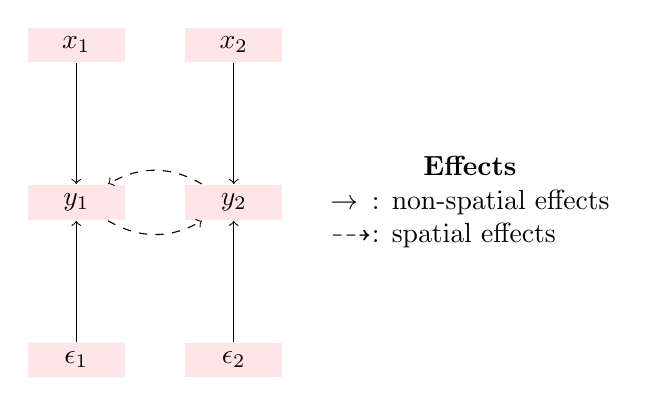
\begin{tikzpicture}
			\node[rectangle, text  width = 1cm, fill = red!10, align = center] (y1) at (-1,0) {$y_1$};
			\node[rectangle, text  width = 1cm, fill = red!10, align = center] (x1) at (-1,2) {$x_1$};
			\node[rectangle, text  width = 1cm, fill = red!10, align = center] (e1) at (-1,-2) {$\epsilon_1$};
			\node[rectangle, text  width = 1cm, fill = red!10, align = center] (y2) at (1, 0) {$y_2$};
			\node[rectangle, text  width = 1cm, fill = red!10, align = center] (x2) at (1,2) {$x_2$};
			\node[rectangle, text  width = 1cm, fill = red!10, align = center] (e2) at (1,-2) {$\epsilon_2$};
			
			\draw[->, solid] (x1) to (y1);
			\draw[->, solid] (x2) to (y2);
			\draw[->, solid] (e1) to (y1);
			\draw[->, solid] (e2) to (y2);
			\draw[dashed, ->] (y1) to[bend right] (y2);
			\draw[dashed, ->] (y2) to[bend right] (y1);

			% Legend
       \node (leyend) at (4, 0){
    \begin{tabular}{l@{: }l}
      \multicolumn{2}{c}{\textbf{Effects}}              \\
      $\rightarrow$                        & non-spatial effects    \\
      $\dashrightarrow$                     & spatial effects  \\
      \end{tabular}
      };
		\end{tikzpicture}
\end{figure}

Figure~\ref{figure:slm} visually illustrates the spatial autoregressive model from Equation~\eqref{eq:slm_model_1}, focusing on two regions. In this representation, the variables $(x_1, x_2)$ and the unobserved terms $(\epsilon_1, \epsilon_2)$ directly influence the dependent variables $y_1$ and $y_2$ in their respective regions. The spatial spillover effects are captured through the influence of $y_1$ on $y_2$ and vice versa. This structure reflects \emph{simultaneity} in the model, highlighting the presence of spatial autocorrelation and spillover effects.

It is important to have different notation forms for the SLM. In vector form, the model can be expressed as:
\begin{equation*}
y_i = \alpha + \rho \underset{(1\times n)}{\vw_i}^\top \underset{(n\times 1)}{\vy} + \epsilon_i, \quad i = 1,\ldots,n,
\end{equation*}
%
where $\vw_i$ is the $i$th row of $\mW$. Additionally, a comprehensive Spatial Lag Model (SLM) specification, considering covariates in matrix form, takes the shape:
\begin{equation}\label{eq:Sar}
\vy  =  \alpha \vones_n+ \rho \mW\vy + \mX\vbeta + \vepsi,
\end{equation}
%
where $\vy$ is a $n\times 1$ vector containing observations on the dependent variable, $\mX$ is an $n\times k$ matrix of observations on the explanatory variables; $\vbeta$ is the $k\times 1$ vector of parameters and $\alpha$ is the constant; and $\vones_n$ is a $n\times 1$ vector of ones.

%====================================
\subsection{Spatial Durbin Model}
%====================================

The Spatial Durbin Model (SDM) is defined as:\index{Spatial durbin model}
\begin{equation}\label{eq:Sdm}
\vy  =  \rho \mW\vy + \alpha \vones_n + \mX\vbeta + \mW\mX\vgamma + \vepsi.
\end{equation}
%
where $\vy$ is the dependent variable, $\rho$ is the spatial autoregressive parameter, $\mW$ is the spatial weights matrix, $\vones_n$ is an $n$-dimensional vector of ones to account for the intercept $\alpha$, $\mX$ is the matrix of explanatory variables, $\mW\mX$ represents the spatially lagged explanatory variables, and $\vepsi$ is the error term.

The SDM extends traditional spatial autoregressive models by including not only the spatially lagged dependent variable ($\mW\vy$) and explanatory variables ($\mX$) but also the spatially lagged explanatory variables ($\mW\mX$). This means that $\vy$ depends on the local (own-region) factors from $\mX$ as well as the same factors averaged over neighboring regions, introducing an additional layer of spatial dependence.

This concept is illustrated in Figure \ref{figure:sdm}. The diagram shows that Region 1 affects Region 2 not only through the spatially lagged dependent variable ($\vy$) but also through the spatially lagged independent and exogenous variables ($\vx$).

\begin{figure}[ht]
	\centering
	\caption{The SDM for Two Regions}\label{figure:sdm}	
		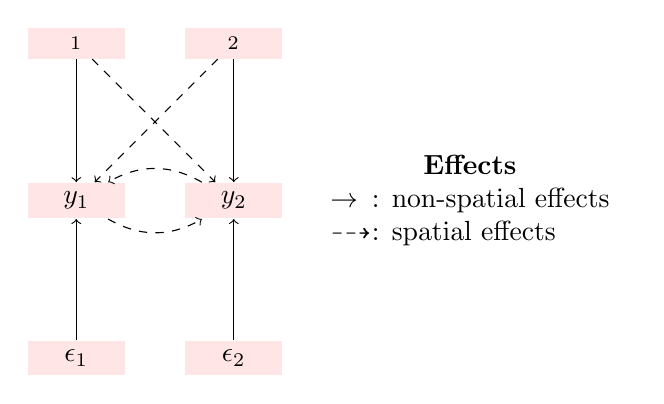
\begin{tikzpicture}
			\node[rectangle, text  width = 1cm, fill = red!10, align = center] (y1) at (-1,0) {$y_1$};
			\node[rectangle, text  width = 1cm, fill = red!10, align = center] (x1) at (-1,2) {$\vx_1$};
			\node[rectangle, text  width = 1cm, fill = red!10, align = center] (e1) at (-1,-2) {$\epsilon_1$};
			\node[rectangle, text  width = 1cm, fill = red!10, align = center] (y2) at (1, 0) {$y_2$};
			\node[rectangle, text  width = 1cm, fill = red!10, align = center] (x2) at (1,2) {$\vx_2$};
			\node[rectangle, text  width = 1cm, fill = red!10, align = center] (e2) at (1,-2) {$\epsilon_2$};

			\draw[->, solid] (x1) to (y1);
			\draw[->, solid] (x2) to (y2);
			\draw[->, solid] (e1) to (y1);
			\draw[->, solid] (e2) to (y2);
			\draw[dashed, ->] (y1) to[bend right] (y2);
			\draw[dashed, ->] (y2) to[bend right] (y1);
			\draw[dashed, ->] (x1) to (y2);
			\draw[dashed, ->] (x2) to (y1);
			% Legend
       \node (leyend) at (4, 0){
    \begin{tabular}{l@{: }l}
      \multicolumn{2}{c}{\textbf{Effects}}              \\
      $\rightarrow$                        & non-spatial effects    \\
      $\dashrightarrow$                     & spatial effects  \\
      \end{tabular}
      };
		\end{tikzpicture}
\end{figure}

Consider an example where $\vy$ represents air pollution levels in different regions. The term $\mW\vy$ implies that air pollution in Region 1 affects pollution in Region 2, and vice versa. If $\mX$ includes population density, the spatially lagged variable $\mW\mX$ captures the effect of population density in Region 1 (or Region 2) on air pollution in the neighboring region.

The SDM is particularly advantageous for calculating marginal effects, as it allows for the decomposition of direct, indirect, and total effects, which will be explored in later sections.

%====================================
\subsection{Spatial Error Model}\label{sec:tax_SEM}
%====================================

Another form of spatial dependence occurs when it operates through the error process, meaning that the errors from different regions exhibit spatial autocorrelation. The Spatial Error Model (SEM) is formulated as\index{Spatial error model}:
\begin{equation}\label{eq:sem_model_comp}
  \begin{aligned}
\vy &= \alpha \vones + \mX\vbeta + \vu, \\
\vu &= \lambda \mW\vu + \vepsi. \\
 \end{aligned}
\end{equation}
%
where $\lambda$ is the autoregressive parameter capturing the spatial dependence in the error lag $\mW\vu$, $\vepsi$ is i.i.d. noise, and $\mW$ is the spatial weights matrix. The parameter $\lambda$ distinguishes the spatial error dependence from the spatial autoregressive coefficient $\rho$ in spatial lag models.

Figure \ref{figure:sem} illustrates the SEM for two regions. The diagram highlights that the error terms ($\epsilon_1$ and $\epsilon_2$) of both regions are interconnected, and the spatial effect operates solely through this relationship.	

\begin{figure}[ht]
	\centering
	\caption{The SEM for two regions}\label{figure:sem}	
		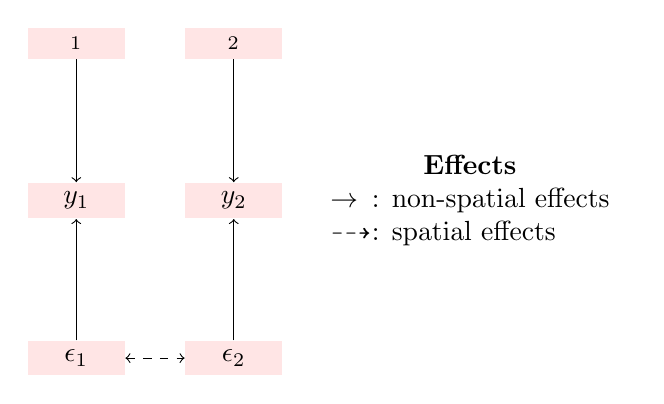
\begin{tikzpicture}
			\node[rectangle, text  width = 1cm, fill = red!10, align = center] (y1) at (-1,0) {$y_1$};
			\node[rectangle, text  width = 1cm, fill = red!10, align = center] (x1) at (-1,2) {$\vx_1$};
			\node[rectangle, text  width = 1cm, fill = red!10, align = center] (e1) at (-1,-2) {$\epsilon_1$};
			\node[rectangle, text  width = 1cm, fill = red!10, align = center] (y2) at (1, 0) {$y_2$};
			\node[rectangle, text  width = 1cm, fill = red!10, align = center] (x2) at (1,2) {$\vx_2$};
			\node[rectangle, text  width = 1cm, fill = red!10, align = center] (e2) at (1,-2) {$\epsilon_2$};

			\draw[->, solid] (x1) to (y1);
			\draw[->, solid] (x2) to (y2);
			\draw[->, solid] (e1) to (y1);
			\draw[->, solid] (e2) to (y2);
			\draw[dashed, <->] (e1) to (e2);

			% Legend
       \node (leyend) at (4, 0){
    \begin{tabular}{l@{: }l}
      \multicolumn{2}{c}{\textbf{Effects}}              \\
      $\rightarrow$                        & non-spatial effects    \\
      $\dashrightarrow$                     & spatial effects  \\
      \end{tabular}
      };
		\end{tikzpicture}
\end{figure}

As noted by \cite{AnselinBera1998}, spatial error dependence can be viewed as a nuisance, with $\lambda$ acting as a nuisance parameter. This reflects spatial autocorrelation in measurement errors or in unaccounted variables that may influence the dependent variable. For instance, it may capture spillovers of omitted variables across spatial units.

Unlike models focusing on explicit spatial or social interaction processes, the SEM accommodates situations where the determinants of the dependent variable are spatially autocorrelated but not explicitly modeled. It can also represent scenarios where unobserved shocks exhibit a spatial pattern. This flexibility makes the SEM useful in dealing with spatially structured errors that arise from omitted variables or other latent spatial processes.
% The spatial diffusion of this model can be analyzed if we consider the reduced form equation. If the matrix $(\mI_n - \lambda\mW)$ is not singular, then \eqref{eq:sem_model_comp} can be written under the following reduced form\index{Spatial error model!reduced form}:
% 
% \begin{equation}
%   \vy =  \alpha \vones + \mX\vbeta + (\mI_n - \lambda\mW)^{-1}\vepsi.
% \end{equation}
% 
% This expression leads to a global spatial diffusion effect, but there is not spatial multiplier effect. The variance-covariance matrix is given by:
% 
% \begin{equation}
%   \begin{aligned}
% \E\left(\left.\vy\vy^\top\right|\mW, \mX\right)  & = \E\left(\left.\vepsi\vepsi^\top\right|\mW, \mX\right) \\
%                  & = \left(\mI_n- \lambda\mW\right)^{-1}\E\left(\left.\vepsi\vepsi^\top\right|\mW, \mX\right)\left(\mI_n- \lambda\mW^\top\right)^{-1}
% \end{aligned}
% \end{equation}

\begin{remark}
Interaction effects among the unobserved terms may also be interpreted to reflect a mechanism to correct rent-seeking politicians for unanticipated fiscal policy changes. See for example \cite{allers2005tax}.
\end{remark}

%=========================
\subsection{Spatial Autocorrelation Model}
%=========================

The Spatial Autocorrelation Model (SAC) is a more general framework that incorporates key features of both the spatial lag and spatial error models discussed earlier. Its structural representation is given by:
\begin{equation*}
  \begin{aligned}
    y_i & = \alpha + \rho    \sum_{j = 1}^n w_{ij} y_j + \sum_{k=1}^K x_{ik}\beta_k + u_i \\
    u_i & = \lambda \sum_{j = 1}^n m_{ij} u_j + \epsilon_i
  \end{aligned}
\end{equation*}
%
or more compactly in matrix form, 
\begin{equation*}
  \begin{aligned}
\vy &= \alpha \vones_n + \rho \mW\vy + \mX\vbeta + \vu, \\
\vu &= \lambda \mM\vu + \vepsi, \\
  \end{aligned}
\end{equation*}
%
where the matrix $\mW$ and $\mM$ are $n\times n$ spatial-weighting matrices.\footnote{This model is also known as SARAR(1, 1) model or Cliff-Ord models because of the impact that \cite{cliff1973spatial}  had on the subsequent literature. Note that SARAR(1, 1) is  a special case of the more general SARAR(p, q) model.} In this model, spatial interactions in the dependent variable and the disturbances are considered. As standard, the spatial weight matrices $\mW$ and $\mM$ are taken to be known and nonsthocastic. These matrices are part of the model definition, and in many applications, $\mM = \mW$. When $\rho = 0$, the model reduces to the SEM. When $\lambda = 0$ the model reduces to the SLM (SAR) specification. Setting $\rho = 0$ and $\lambda = 0$ causes the model to reduce to a linear regression model with exogenous variables. 

A broader taxonomy of spatial models is shown in Figure \ref{fig:taxonomy}. The most comprehensive model in this framework is the General Nesting Spatial Model (GNS or Manski's Model), which includes spatial dependence in the dependent variable, the explanatory variables, and the error term. Different restrictions on the GNS model yield various spatial model specifications, as detailed below.

\begin{figure}[h]
\caption{Taxonomy of spatial models}
\label{fig:taxonomy}
\centering
\begin{tikzpicture}[scale = 0.8]
			\node[rectangle, text  width = 5cm, fill = red!10, align = center] (gns) at (0,0) {\scriptsize General nesting spatial model \\
			\begin{eqnarray*}
			\vy &=& \rho\mW\vy + \mX\vbeta + \mW\mX\vgamma + \vu \\
			\vu &=& \lambda\mW\vu + \vepsi
			\end{eqnarray*}};
			
			\node[rectangle, text  width = 3cm, fill = red!10, align = center] (sac) at (6,4) {\scriptsize  SAC \\
			\begin{eqnarray*}
			\vy &=& \rho\mW\vy + \mX\vbeta + \vu \\
			\vu &=& \lambda\mW\vu + \vepsi
			\end{eqnarray*}};
			
			\node[rectangle, text  width = 3cm, fill = red!10, align = center] (sdm) at (6,0) {\scriptsize  Spatial durbin model \\
			\begin{equation*}
			\vy = \rho\mW\vy + \mX\vbeta + \mW\mX\vgamma + \vepsi
			\end{equation*}};
			
			\node[rectangle, text  width = 3cm, fill = red!10, align = center] (sde) at (6,-4) {\scriptsize Spatial durbin error model \\
			\begin{eqnarray*}
			\vy &=& \mX\vbeta + \mW\mX\vgamma + \vu \\
			\vu &=& \lambda\mW\vu + \vepsi
			\end{eqnarray*}};
			
			\node[rectangle, text  width = 3cm, fill = red!10, align = center] (slm) at (12,4) {\scriptsize Spatial Lag Model \\
			\begin{equation*}
			\vy = \rho\mW\vy + \mX\vbeta + \vepsi
			\end{equation*}};
			
			\node[rectangle, text  width = 3cm, fill = red!10, align = center] (slx) at (12,0) {\scriptsize SLX \\
			\begin{equation*}
			\vy = \mX\vbeta + \mW\mX\vgamma + \vepsi
			\end{equation*}};
			
			\node[rectangle, text  width = 3cm, fill = red!10, align = center] (sem) at (12,-4) {\scriptsize Spatial error model \\
			\begin{eqnarray*}
			\vy &=& \mX\vbeta + \vu \\
			\vu &=& \lambda\mW\vu + \vepsi
			\end{eqnarray*}};
			
			\node[rectangle, text  width = 2cm, fill = red!10, align = center] (ols) at (16,0) {\scriptsize OLS \\
			\begin{equation*}
			\vy = \mX\vbeta + \vepsi
			\end{equation*}};

			\draw (gns) -- (sac) node [->, solid, midway, above, sloped] {\scriptsize $\vgamma = 0$};
			\draw (gns) -- (sdm) node [->, solid, midway, above, sloped] {\scriptsize $\lambda = 0$};
			\draw (gns) -- (sde) node [->, solid, midway, above, sloped] {\scriptsize $\rho = 0$};
			\draw (sac) -- (slm) node [->, solid, midway, above, sloped] {\scriptsize $\lambda = 0$};
			\draw (sac) -- (sem) node [->, solid, near end, above, sloped] {\scriptsize $\rho = 0$};
			\draw (sdm) -- (slx) node [->, solid, near end, above, sloped] {\scriptsize $\rho = 0$};
			\draw (sde) -- (slx) node [->, solid, near start, above, sloped] {\scriptsize $\lambda = 0$};
			\draw (sdm) -- (slm) node [->, solid, midway, above, sloped] {\scriptsize $\gamma = 0$};
			\draw (sdm) -- (sem) node [->, solid, midway, above, sloped] {\scriptsize $\gamma = -\rho\beta$};
			\draw (sde) -- (sem) node [->, solid, midway, above, sloped] {\scriptsize $\gamma = 0$};
			\draw (slm) -- (ols) node [->, solid, midway, above, sloped] {\scriptsize $\rho = 0$};
			\draw (slx) -- (ols) node [->, solid, midway, above, sloped] {\scriptsize $\gamma = 0$};
			\draw (sem) -- (ols) node [->, solid, midway, above, sloped] {\scriptsize $\lambda = 0$};
\end{tikzpicture}
\end{figure}

Starting with the GNS model:

\begin{itemize}
  \item Imposing the restriction $\vgamma = \vzeros$ leads to the SAC model that includes both a spatial lag for the dependent variable and spatial lag for the error term, but excludes the influence of the spatially lagged explanatory variables. 
  \item Imposing the restriction $\lambda = 0$ leads to the SDM.
  \item Imposing the restriction $\rho = 0$ leads to the Spatial Durbin Error Model (SDEM). 
\end{itemize}

Starting with the SDM:

\begin{itemize}
  \item The so-called common factor parameter restrictions $(\vgamma = -\rho\vbeta)$ yields the spatial error regression model (SEM) specification that assumes that externalities across spatial unites are mostly a nuisance spatial dependence problem caused by the regional transmission of random shocks. 
  \item Imposing the restriction $\gamma = 0$ leads to the spatial lag model (SLM), whereas the restriction $\rho = 0$ results in a least-squares spatially lagged $\mX$ regression model (labeled SLX) that assumes independence between regions in the dependent variable, but includes characteristics from neighboring regions in the form of spatially lagged explanatory variables.  
\end{itemize}

Finally, if $\rho = \lambda = 0$ and $\vtheta = 0$, then we obtain the traditional linear regression model. 

%-------------------------------------------------------------------------
\section{Reduced Form and Parameter Space}\index{Reduced form!Spatial lag model}
%-------------------------------------------------------------------------

An important distinction in the context of spatial models is the difference between structural and reduced form model. The reduced form expresses the endogenous variables as functions of the exogenous variables. In contrast, the structural form is the `behavioral model' that defines the relationship between the vaiables in the system.  

For example, Equation \eqref{eq:Sar} represents the structural model for the SLM, where both exogenous and endogenous variables are related to the dependent variable $\vy$. This form reflects the theoretical framework that captures the underlying relationship between the variables. 

However, it is often more insightful to consider how the dependent variable is generated, which is referred to as the \textbf{data generating process} (DGP). The DGP represents the empirical process that gives rise to the observed data. By solving the structural model in Equation \eqref{eq:Sar} for the endogenous variables, $\vy$, yields the reduced-form model. 

The implied DGP or ``reduced form equation'' for the SLM given in Equation \eqref{eq:Sar} is:
\begin{equation}\label{eq:Sar_dgp}
\vy  =  \left(\mI_n - \rho \mW\right)^{-1}\left(\alpha \vones_n + \mX\vbeta\right) + \left(\mI_n - \rho \mW\right)^{-1}\vepsi,
\end{equation}
%
which shows that any spatially lagged dependent variable is no longer present on the right-hand side. This equation illustrate the simultaneous nature of the spatial autoregressive process.

\begin{remark}
The \textbf{reduced form} of a system of equations is the result of solving the system for the \textbf{endogenous variables}. This gives the latter as functions of the exogenous variables, if any. For example, the general expression of a structural form is $f(\vy, \mX, \vepsi) = \vzeros$, whereas the reduced form of this model is given by $\vy = g(\mX, \vepsi)$, with $g$ as function. 
\end{remark}

Without restrictions on $(\mI_n-\rho\mW)$---and $\left(\alpha \vones_n + \mX\vbeta\right)$---the coefficients cannot be identified from data. In other words, to identify the true coefficients from data, we need $(\mI_n-\rho\mW)$ to be invertible. From linear algebra, a matrix $\mA$ is invertible if $\det(\mA)\neq 0$. Thus, for the reduced from to be valid we require that $\det(\mI_n -\rho\mW)\neq 0$. The question then becomes: for which values of $\rho$ lead to a non-singular $(\mI_n -\rho\mW)$? 

%For \textbf{symmetric} matrices, the compact open interval for $\rho \in \left( \omega_{min}^{-1}, \omega_{max}^{-1}\right)$ will lead to a symmetric positive definite $(\mI_n -\rho\mW)$, where $\omega_{min}$ and $\omega_{max}$ are the minimum and maximum eigen value of $\mW$, respectively. This gives rise to the following Theorem:

The following Lemma from \cite{kelejian2010specification} establishes a bound for $\rho$:

%---------------------------
\begin{lemma}[Bounds for $\rho$ \citep{kelejian2010specification}]\label{lemma:bound-rho-kp}
Let $\tau$ denote the spectral radius of $\mW$, defined as:
\begin{equation*}
\tau = \max\left\lbrace |\omega_1|, \ldots, |\omega_n| \right\rbrace,
\end{equation*}
%
where $\omega_1, \ldots, \omega_n$ denote the eigenvalues of $\mW$. Then $\mI_n - \rho\mW$ is nonsingular for all $\rho$ in the interval $(-1/\tau, 1/\tau)$. 
\end{lemma}
%---------------------------

When $\rho$ is restricted to the interval $(-1/\tau, 1/\tau)$, all eigenvalues of $\rho\mW$ are guaranteed to have absolute values less than one. A related result, frequently used in the literature, is presented below:

%%%%%%%%%%%%%%%%%%%%%%%%%%%%%%%%%%%%%%%
\begin{lemma}[Invertibility]\index{Weight matrix!Invertibility}\index{eigen values}\label{lemma:inveribility}
Let $\mW$ be a weighting matrix, such that $w_{ii} = 0$ for all $i = 1,\ldots,n$, and assume that all of the roots of $\mW$ are real. Assume also that $\mW$ is not row normalized. Let $\omega_{min}$ and $\omega_{max}$ be the minimum and maximum eigen value of $\mW$. Assume also that $\omega_{max} > 0$ and $\omega_{min} < 0$. Then $\left(\mI_n - \rho\mW\right)$ is nonsingular for all:
\begin{equation*}
  \omega_{min}^{-1} < \rho < \omega_{max}^{-1}
\end{equation*}
\end{lemma}
%%%%%%%%%%%%%%%%%%%%%%%%%%%%%%%%%%%%

As \cite{kelejian2010specification} explain, Lemma \ref{lemma:inveribility} holds only when all eigenvalues of $\mW$ are real. However, non-symmetric matrices typically have complex eigenvalues, making Lemma \ref{lemma:bound-rho-kp} more general.

To facilitate interpretation, $\mW$ is often normalized so that each row sums to unity. This row-normalization ensures nonnegative weights between 0 and 1, which allows $\mW$ to be interpreted as a row-stochastic matrix that averages neighboring values. According to Theorem \ref{teo:eigen_values} (Eigenvalues of Row-Stochastic Matrix), the eigenvalues of such a row-stochastic matrix $\mW$ have absolute values less than or equal to one. This result, combined with Lemma \ref{lemma:bound-rho-kp}, implies $\rho \in (1/\omega_{\textrm{min}}, 1)$.

However, interpreting $\rho$ as a conventional correlation coefficient between $\vy$ and its spatial lag $\mW\vy$ can be misleading. The parameter space of $\rho$ depends on the normalization of $\mW$. For instance, standardization methods other than row-normalization may yield different bounds for $\rho$. 

%----------------------------
\begin{lemma}[Invertibility of Row-Normalized $\mW$ matrix]\label{lemma:invert-W-row}
If $\mW$ is row-normalized, then  $\left(\mI_n - \rho\mW\right)^{-1}$ exists for all $\left|\rho \right| < 1$
\end{lemma}
%----------------------------

Despite its popularity, row-normalization has drawbacks. As discussed in Section \ref{sec:spatial_lag_var}, it alters the internal structure of $\mW$, complicating inter-row comparisons. To address this, scalar normalization (multiplying $\mW$ by a constant $a$) can be applied. This approach preserves the relationships between rows and removes unit-of-measure effects. Let:
\begin{equation*}
  \begin{aligned}
    a & = \min \left\lbrace r, c \right\rbrace \\
    r & = \max_i \sum_j \left|w_{ij}\right|\quad \mbox{maximal row sum of the absolute values} \\
    c & = \max_j \sum_i \left|w_{ij}\right|\quad \mbox{maximal column sum of the absolute values}.
  \end{aligned}
\end{equation*}

Then, assuming that the elements of $\mW$ are nonegative, $(\mI_n - \rho\mW)$ will be nonsingular for all $\left|\rho\right| < 1/a$. Note that this normalization has the advantage of ensuring that the resulting spatial weights, $w_{ij}$, are all between 0 and 1, and hence can still be interpreted as relative influence intensities. This could be taken as the parameter space.\index{Parameter space} 

This is an important result because a model which has a weighting matrix which is not row normalized can always be normalized in such a way that the inverse needed to solve the model will exists in an easily established region. 


\begin{remark}
For further details on normalizing $\mW$ and the parameter space of $\rho$ see \citet[][section 2.4]{elhorst2014spatial} and \citet[][section 2.2]{kelejian2010specification}
\end{remark}

When $\mI_n - \rho\mW$ is nonsingular, it can be expressed as an infinite series, commonly referred to as the Leontief expansion:

%----------------------
\begin{lemma}[Leontief Expansion]\label{lemma:Leontief}\index{Leontief expansion}
If $\mI - \rho \mW$ is nonsingular, then
	\begin{equation*}
	(\mI - \rho \mW)^{-1} = \sum_{i = 0} ^{\infty}(\rho \mW)^{i}
	\end{equation*}
\end{lemma}
%----------------------

Using Lemma \ref{lemma:Leontief} (Leontief Expansion), the reduced form for the SLM in Equation \eqref{eq:Sar_dgp} can be written as:
\begin{equation}\label{eq:infinite_series_slm}
  \begin{aligned}
      \vy  = &\left(\mI_n + \rho\mW + \rho^2\mW^2 + \ldots \right)\left(\alpha \vones_n + \mX\vbeta\right) + \left(\mI_n + \rho\mW + \rho^2\mW^2 + \ldots\right)\vepsi, \\
           = & \alpha\vones_n + \rho\mW\vones_n\alpha + \rho^2\mW^2\vones_n\alpha + \ldots + \mX\vbeta + \rho\mW\mX\vbeta + \rho^2\mW^2\mX\vbeta + \ldots \\
          & + \vepsi + \rho\mW\vepsi + \rho^2\mW^2\vepsi.
  \end{aligned}
\end{equation}

Expression \eqref{eq:infinite_series_slm} can be simplified since the infinite series:
\begin{equation*}
\alpha\vones_n + \rho\mW\vones_n\alpha + \rho^2\mW^2\vones_\alpha + \ldots \to \frac{\vones_n\alpha}{\left(1 - \rho\right)},
\end{equation*}
%
since $\alpha$ is a scalar, the parameter $\left|\rho\right|  < 1$, and $\mW$ is row-stochastic. By definition $\mW\vones_n = \vones_n$ and therefore $\mW\mW\vones_n = \mW\vones_n = \vones$. Consequently, $\mW^l\vones_n = \vones_n$ for $l\geq 0$ (recall that $\mW^0 = \mI_n$). This allows us to write:
\begin{equation*}
\vy = \frac{1}{(1-\rho)}\vones_n\alpha + \mX\vbeta + \rho\mW\mX\vbeta + \rho^2\mW^2\mX\vbeta + \ldots + \vepsi + \rho\mW\vepsi + \rho^2\mW^2\vepsi + \ldots
\end{equation*}

This expansion reveals two effects: a multiplier effect affecting the explanatory variables and a spatial diffusion effect affecting the error terms. With respect to the explanatory variables, this expression means that, on average, the value of $\vy$ at one location $i$ is not only explained by the values of the explanatory variables associated to this location but also by those associated to all other locations (neighbors or not) via the inverse spatial transformation $\left(\mI_n - \rho \mW\right)^{-1}$. This spatial multiplier effect decreases with distance. This can be seen if we consider the powers of $\mW$ in the series expansion of $\left(\mI_n - \rho \mW\right)^{-1}$.\index{Multiplier effect} 

With respect to the error process, this expression means that a random (unobserved) shock in a location $i$ not only affects the value of $y$ in this location but also has an impact on the values of $y$ in all other locations via the same spatial inverse transformation. To see this, recall that $\mW^2$ will reflect second-order contiguous neighbors, those that are neighbors to the first-order neighbors (review Section \ref{sec:HSO}). Since the neighbor of the neighbor (second-order neighbor) to an observation $i$ includes observation $i$ itself, $\mW^2$ has positive elements on the diagonal when each observations has at least one neighbor. That is, higher-order spatial lags can lead to a connectivity relation for an observations $i$ such that $\mW\vepsi$ will extract observations from the vector $\vepsi$ that point back to the observation $i$ itself. This implies that there exists a simultaneous feedback. This diffusion effect also declines with distance. We will explore this mechanism more deeply in Section \ref{sec:interpretation}.

Considering the reduced form Equation (\ref{eq:Sar_dgp}), we might be able to find the mean and variance-covariance matrix of the complete system as function of exogenous variables. The expectation is given by:
\begin{equation}\label{eq:expected_value_slm}
  \begin{aligned}
\E(\vy|\mX,\mW) & = \E\left[\left.\left(\mI_n - \rho \mW\right)^{-1}\left(\alpha \vones_n + \mX\vbeta\right) + \left(\mI_n - \rho \mW\right)^{-1}\vepsi\right|\mX,\mW\right] \\
                & = \left(\mI_n - \rho \mW\right)^{-1}\left(\alpha \vones_n + \mX\vbeta\right).
\end{aligned}
\end{equation}

From Equation \eqref{eq:Sar_dgp}, we derive the variance-covariance matrix of $\vy$:
\begin{equation*}
  \begin{aligned}
    \var\left(\left.\vy\right|\mW, \mX\right) & = \E\left(\left.\vy\vy^\top\right|\mW,\mX\right) \\ 
                               & = \left(\mI_n - \rho\mW\right)^{-1}\E\left(\left.\vepsi\vepsi^\top\right|\mW, \mX\right)\left(\mI_n- \rho\mW^\top\right)
  \end{aligned}
\end{equation*}

This $n\times n$ variance-covariance matrix is full, which implies that each location is correlated with every other location in the system. However, this correlation decreases with distance. Since we have not assumed anything about the error variance, we can say that $\E\left(\left.\vepsi\vepsi^\top\right|\mW, \mX\right)$ is a full matrix, say $\mOmega_{\epsilon}$. This covers the possibility of heteroskedasticity, spatial autocorrelation, or both. In absence of either of these complications, the variance matrix simplifies to the usual $\sigma^2\mI_n$.

\begin{example}[County homicide rates in US]
In the criminology literature there has been a great emphasis of spatial diffusion of crime. The idea is that criminal violence may spread geographically via a diffusion process. For example, some researchers suggests that certain social processes such as illegal drug markets and gang rivalries may be important for explaining the pattern and mechanisms of the spread of homicides \citep{cohen1999diffusion}. 

In particular, empirical literature has focused on homicide rates and their determinants using the following OLS specification:

\begin{equation*}
y_i = \vx_i^\top\vbeta + \epsilon_i\quad i = 1, ..., n,
\end{equation*}
%
where $y_i$ is the homicide rate in spatial unit $i$ and $\vx_i$ is a $k\times 1$ set of covariates that explain homicide rates across spatial units. However, this model does not allow capturing the idea of spatial diffusion and spatial effects of homicide rates. For example, \cite{baller2001structural}, after rejecting the null hypothesis of spatial randomness on homicide rates, propose (among other spatial models) the following SLM process for modeling homicide rates using a county-level data for the decennial years in the 1960 to 1990 time period:

\begin{equation*}
\vy  =  \alpha \vones_n + \rho \mW\vy + \mX\vbeta + \epsilon,
\end{equation*}
%
where $\vy$ is the homicide rates for the US counties, $\mX$ includes a deprivation, population density, median age, the unemployment rate, percent divorced, and a Southern dummy variable based on census definitions.  As explained by \cite{baller2001structural}, if homicides rates are determined solely by the structural factors included in the $\mX$ matrix, there should be no spatial patterning of homicide beyond that created by socio-demographic similarities of geographically proximate counties. If this is the case, once all $x_k$ are included in the model, the spatial relationship between $y_i$ and $y_j$ will become nonsignificant. This implies that $\rho = 0$.

This is the model most compatible with common notions of diffusion processes because it implies an influence of neighbors' homicide rates that is not simply an artifact of measured or unmeasured independent variables. Rather, homicide events in one place actually increase the likelihood of homicides in nearby locales. 
\end{example}

%-------------------------------------------------------------------------
\subsection{Eigenvalues in R}
%-------------------------------------------------------------------------

Computing eigenvalues is a crucial step in the estimation of spatial models, particularly when using Maximum Likelihood procedures. In this section, we demonstrate how to compute the eigenvalues of a spatial weight matrix $\mW$ in R, along with some of their properties.

First, we create an artificial spatial weight matrix using functions from the \pkg{spdep} package:

\begin{knitrout}
\definecolor{shadecolor}{rgb}{0.969, 0.969, 0.969}\color{fgcolor}\begin{kframe}
\begin{alltt}
\hlcom{# Create a queen W matrix}
\hlkwd{library}\hldef{(}\hlsng{"spdep"}\hldef{)}
\hldef{Wl.queen} \hlkwb{<-} \hlkwd{cell2nb}\hldef{(}\hlnum{3}\hldef{,} \hlnum{3}\hldef{,} \hlkwc{type} \hldef{=} \hlsng{"queen"}\hldef{)}
\hlkwd{summary}\hldef{(Wl.queen)}
\end{alltt}
\begin{verbatim}
## Neighbour list object:
## Number of regions: 9 
## Number of nonzero links: 40 
## Percentage nonzero weights: 49.38272 
## Average number of links: 4.444444 
## Link number distribution:
## 
## 3 5 8 
## 4 4 1 
## 4 least connected regions:
## 1:1 3:1 1:3 3:3 with 3 links
## 1 most connected region:
## 2:2 with 8 links
\end{verbatim}
\end{kframe}
\end{knitrout}

The function \code{cell2nb} from \pkg{spdep} package generates a list of neighbors for a grid of cells. Here, we define a grid with 3 rows and 3 columns, resulting in a total of 9 regions. Since \code{type = "queen"} is specified, the neighbors include those sharing either an edge or a vertex, consistent with a regular grid spatial structure. The resulting object is of class \code{nb}, representing a list of neighbors.

To proceed with matrix computations, we convert this \code{nb} object into a spatial weight matrix of class \code{matrix}:
\begin{knitrout}
\definecolor{shadecolor}{rgb}{0.969, 0.969, 0.969}\color{fgcolor}\begin{kframe}
\begin{alltt}
\hlcom{# From nb to matrix}
\hldef{W.queen} \hlkwb{<-} \hlkwd{nb2mat}\hldef{(Wl.queen)}
\hlkwd{round}\hldef{(W.queen,} \hlnum{3}\hldef{)}
\end{alltt}
\begin{verbatim}
##       1:1   2:1   3:1   1:2   2:2   3:2   1:3   2:3   3:3
## 1:1 0.000 0.333 0.000 0.333 0.333 0.000 0.000 0.000 0.000
## 2:1 0.200 0.000 0.200 0.200 0.200 0.200 0.000 0.000 0.000
## 3:1 0.000 0.333 0.000 0.000 0.333 0.333 0.000 0.000 0.000
## 1:2 0.200 0.200 0.000 0.000 0.200 0.000 0.200 0.200 0.000
## 2:2 0.125 0.125 0.125 0.125 0.000 0.125 0.125 0.125 0.125
## 3:2 0.000 0.200 0.200 0.000 0.200 0.000 0.000 0.200 0.200
## 1:3 0.000 0.000 0.000 0.333 0.333 0.000 0.000 0.333 0.000
## 2:3 0.000 0.000 0.000 0.200 0.200 0.200 0.200 0.000 0.200
## 3:3 0.000 0.000 0.000 0.000 0.333 0.333 0.000 0.333 0.000
## attr(,"call")
## nb2mat(neighbours = Wl.queen)
\end{verbatim}
\end{kframe}
\end{knitrout}

The resulting matrix is row-normalized, meaning that the sum of each row equals one. We can verify this as follows:
\begin{knitrout}
\definecolor{shadecolor}{rgb}{0.969, 0.969, 0.969}\color{fgcolor}\begin{kframe}
\begin{alltt}
\hlcom{# Compute row-sums}
\hlkwd{rowSums}\hldef{(W.queen)}
\end{alltt}
\begin{verbatim}
## 1:1 2:1 3:1 1:2 2:2 3:2 1:3 2:3 3:3 
##   1   1   1   1   1   1   1   1   1
\end{verbatim}
\end{kframe}
\end{knitrout}

Additionally, note that this matrix is not symmetric. We can confirm this property using:
\begin{knitrout}
\definecolor{shadecolor}{rgb}{0.969, 0.969, 0.969}\color{fgcolor}\begin{kframe}
\begin{alltt}
\hlcom{# Check whether the matrix is symmetric}
\hldef{is.sym} \hlkwb{<-} \hlkwd{all}\hldef{(W.queen} \hlopt{==} \hlkwd{t}\hldef{(W.queen))}
\hldef{is.sym}
\end{alltt}
\begin{verbatim}
## [1] FALSE
\end{verbatim}
\end{kframe}
\end{knitrout}

The \code{eigen} function in R computes the eigenvalues and eigenvectors of a matrix. It returns a named list with two components: \code{values} (the eigenvalues) and \code{vectors} (the eigenvectors). To illustrate, we compute the eigenvalues of the previously defined spatial weight matrix:

\begin{knitrout}
\definecolor{shadecolor}{rgb}{0.969, 0.969, 0.969}\color{fgcolor}\begin{kframe}
\begin{alltt}
\hlcom{# Obtain eigenvalues}
\hldef{values} \hlkwb{<-} \hlkwd{eigen}\hldef{(W.queen,} \hlkwc{symmetric} \hldef{= is.sym)}\hlopt{$}\hldef{values}
\hldef{values}
\end{alltt}
\begin{verbatim}
## [1]  1.000000e+00 -4.527525e-01 -4.000000e-01  3.651484e-01 -3.651484e-01
## [6]  3.651484e-01 -3.651484e-01 -1.472475e-01 -2.259287e-16
\end{verbatim}
\begin{alltt}
\hlkwd{range}\hldef{(values)}
\end{alltt}
\begin{verbatim}
## [1] -0.4527525  1.0000000
\end{verbatim}
\end{kframe}
\end{knitrout}

The eigenvalues are returned in decreasing order. For the spatial weight matrix \code{W.queen}, all eigenvalues are real. The minimum eigenvalue is approximately -0.45, while the maximum eigenvalue is 1, corroborating the fact that if $\mW$ is row-normalized, then $|\vomega| \leq 1$.

Since $\mW$ is row-normalized, and  according to Lemma \ref{lemma:invert-W-row}, $\mI_n - \rho\mW$ is invertible if $|\rho| < 1$. Note that if $\rho = 1$, then the matrix is nonsingular as shown in the following lines
\begin{knitrout}
\definecolor{shadecolor}{rgb}{0.969, 0.969, 0.969}\color{fgcolor}\begin{kframe}
\begin{alltt}
\hlkwd{solve}\hldef{(}\hlkwd{diag}\hldef{(}\hlnum{9}\hldef{)} \hlopt{-} \hlnum{1} \hlopt{*} \hldef{W.queen)}
\end{alltt}


{\ttfamily\noindent\bfseries\color{errorcolor}{\#\# Error in solve.default(diag(9) - 1 * W.queen): system is computationally singular: reciprocal condition number = 3.6909e-18}}\end{kframe}
\end{knitrout}


Next, we compute the eigenvalues for a rook spatial weight matrix:
\begin{knitrout}
\definecolor{shadecolor}{rgb}{0.969, 0.969, 0.969}\color{fgcolor}\begin{kframe}
\begin{alltt}
\hldef{W.rook} \hlkwb{<-} \hlkwd{nb2mat}\hldef{(}\hlkwd{cell2nb}\hldef{(}\hlnum{3}\hldef{,} \hlnum{3}\hldef{,} \hlkwc{type} \hldef{=} \hlsng{"rook"}\hldef{))}
\hldef{is.sym} \hlkwb{<-} \hlkwd{all}\hldef{(W.rook} \hlopt{==} \hlkwd{t}\hldef{(W.rook))}
\hldef{values} \hlkwb{<-} \hlkwd{eigen}\hldef{(W.rook,} \hlkwc{symmetric} \hldef{= is.sym)}\hlopt{$}\hldef{values}
\hlkwd{range}\hldef{(values)}
\end{alltt}


{\ttfamily\noindent\bfseries\color{errorcolor}{\#\# Error in min(x, na.rm = na.rm): invalid 'type' (complex) of argument}}\end{kframe}
\end{knitrout}

For the rook spatial weight matrix, the minimum eigenvalue is -1, and the maximum eigenvalue is 1. This highlights a difference in the spectral properties of rook versus queen spatial weight matrices.

Another approach to constructing spatial weight matrices, particularly for Monte Carlo studies, is the $k$-ahead and $k$-behind criterion in a circular world, as proposed by \citet{kelejian1999generalized}. In this framework, each spatial unit is assumed to have $k$ neighbors ahead of it and $k$ neighbors behind it in the sample order. For example, we can create such a matrix with $k = 2$ using the \code{circular} function from the \pkg{sphet} package:
\begin{knitrout}
\definecolor{shadecolor}{rgb}{0.969, 0.969, 0.969}\color{fgcolor}\begin{kframe}
\begin{alltt}
\hlkwd{library}\hldef{(}\hlsng{"sphet"}\hldef{)}
\hldef{W.cir} \hlkwb{<-} \hlkwd{nb2mat}\hldef{(}\hlkwd{circular}\hldef{(}\hlnum{3}\hldef{,} \hlnum{3}\hldef{,} \hlnum{2}\hldef{))}
\hldef{W.cir}
\end{alltt}
\begin{verbatim}
##      1:1  2:1  3:1  1:2  2:2  3:2  1:3  2:3  3:3
## 1:1 0.00 0.25 0.25 0.00 0.00 0.00 0.00 0.25 0.25
## 2:1 0.25 0.00 0.25 0.25 0.00 0.00 0.00 0.00 0.25
## 3:1 0.25 0.25 0.00 0.25 0.25 0.00 0.00 0.00 0.00
## 1:2 0.00 0.25 0.25 0.00 0.25 0.25 0.00 0.00 0.00
## 2:2 0.00 0.00 0.25 0.25 0.00 0.25 0.25 0.00 0.00
## 3:2 0.00 0.00 0.00 0.25 0.25 0.00 0.25 0.25 0.00
## 1:3 0.00 0.00 0.00 0.00 0.25 0.25 0.00 0.25 0.25
## 2:3 0.25 0.00 0.00 0.00 0.00 0.25 0.25 0.00 0.25
## 3:3 0.25 0.25 0.00 0.00 0.00 0.00 0.25 0.25 0.00
## attr(,"call")
## nb2mat(neighbours = circular(3, 3, 2))
\end{verbatim}
\begin{alltt}
\hlkwd{all}\hldef{(W.cir} \hlopt{==} \hlkwd{t}\hldef{(W.cir))}
\end{alltt}
\begin{verbatim}
## [1] TRUE
\end{verbatim}
\begin{alltt}
\hldef{values} \hlkwb{<-} \hlkwd{eigen}\hldef{(W.cir,} \hlkwc{symmetric} \hldef{=} \hlkwd{all}\hldef{(W.cir} \hlopt{==} \hlkwd{t}\hldef{(W.cir)))}\hlopt{$}\hldef{values}
\hldef{values}
\end{alltt}
\begin{verbatim}
## [1]  1.00000000  0.46984631  0.46984631 -0.08682409 -0.08682409 -0.38302222
## [7] -0.38302222 -0.50000000 -0.50000000
\end{verbatim}
\begin{alltt}
\hlkwd{range}\hldef{(values)}
\end{alltt}
\begin{verbatim}
## [1] -0.5  1.0
\end{verbatim}
\end{kframe}
\end{knitrout}

In this example, each spatial unit has $2k$ neighbors (two ahead and two behind). The eigenvalues for this matrix can provide insights into the connectivity and spatial structure defined by this criterion.

%-------------------------------------------------------------------------
\subsection{Generate spatial DGP in R}
%-------------------------------------------------------------------------

To construct a DGP of a spatial model, we first define the reduced form of the model. Consider the SLM with
\begin{equation*}
\vy = \left(\mI_n - \rho\mW\right)^{-1}\left(\beta_0\vones_n + \beta_1\vx + \vepsi\right), 
\end{equation*}
%
where $\vones_n$ is an $n\times 1$ vector of ones and the elements of the vector $\vx$ are normally distributed with mean 0 and standard deviation 1. The parameter $\beta_0$ is set to 1, while $\beta_1 = 2$. The error term is normally distributed with mean zero and standard deviation one. The spatial autoregressive parameter is set to $\rho = 0.6$. 
The following lines create this DGP for a sample size of $n = 49$ using a circular spatial weight matrix:
\begin{knitrout}
\definecolor{shadecolor}{rgb}{0.969, 0.969, 0.969}\color{fgcolor}\begin{kframe}
\begin{alltt}
\hlcom{# Set the random seed}
\hlkwd{set.seed}\hldef{(}\hlnum{1}\hldef{)}

\hlcom{# True parameters}
\hldef{b0}  \hlkwb{<-} \hlnum{1}
\hldef{b1}  \hlkwb{<-} \hlnum{2}
\hldef{rho} \hlkwb{<-} \hlnum{0.6}

\hlcom{# Sample size and W matrix}
\hldef{n}     \hlkwb{<-} \hlnum{49}
\hldef{W.cir} \hlkwb{<-} \hlkwd{nb2mat}\hldef{(}\hlkwd{circular}\hldef{(}\hlkwd{sqrt}\hldef{(n),} \hlkwd{sqrt}\hldef{(n),} \hlnum{3}\hldef{))}

\hlcom{# Generate random variables}
\hldef{x} \hlkwb{<-} \hlkwd{rnorm}\hldef{(n,} \hlkwc{mean} \hldef{=} \hlnum{0}\hldef{,} \hlkwc{sd} \hldef{=} \hlnum{1}\hldef{)}
\hldef{epsilon} \hlkwb{<-} \hlkwd{rnorm}\hldef{(n,} \hlkwc{mean} \hldef{=} \hlnum{0}\hldef{,} \hlkwc{sd} \hldef{=} \hlnum{1}\hldef{)}

\hlcom{# Generate dependent variable}
\hldef{y} \hlkwb{<-} \hlkwd{solve}\hldef{(}\hlkwd{diag}\hldef{(n)} \hlopt{-}  \hldef{rho} \hlopt{*} \hldef{W.cir)} \hlopt \hldef{(b0} \hlopt{+} \hldef{b1} \hlopt{*} \hldef{x} \hlopt{+} \hldef{epsilon)}
\end{alltt}
\end{kframe}
\end{knitrout}

%==============================================
\section{Motivation of Spatial Models}\label{sec:motivation}
%==============================================

\subsection{SLM as a Long-run Equilibrium}\label{sec:SLM_lre}

A Spatial Lag Model (SLM) can be interpreted as a system of simultaneous dependencies over time that converges to a new steady-state equilibrium, even when using a cross-sectional dataset \citep{lesage2010introduction}. To demonstrate this, consider the vector of the dependent variable at time $t$, denoted by $\vy_t$. Assume that this variable is determined by a spatial autoregressive process, where the current value depends on the spatially lagged values of the dependent variable from neighboring observations. This introduces a time lag in the average values of the neighboring dependent variables observed during the previous period, $\mW\vy_{t-1}$. We can also include the current period's own-region characteristics $\mX_t$ in the model. If the characteristics of regions remain relatively fixed over time, we can express $\mX_t = \mX$.

For illustration, consider a model where pollution is the dependent variable $\vy_t$, which depends on the past period's pollution values from neighboring regions, $\mW\vy_{t-1}$. The appropriate model in this case would be:
\begin{equation}\label{eq:slm_with_time}
\vy_t = \rho \mW\vy_{t-1} + \mX\vbeta + \vepsi_t.
\end{equation}

We can substitute $\vy_{t-1}$ from the right-hand side of equation \eqref{eq:slm_with_time} as:
\begin{equation*}
\vy_{t-1} = \rho \mW\vy_{t-2} + \mX\vbeta + \vepsi_{t-1},
\end{equation*}
%
resulting in:
\begin{equation}\label{eq:recur_2}
\begin{aligned}
\vy_t  = & \mX\vbeta +\rho\mW\left(\mX\vbeta + \rho \mW\vy_{t-2} + \vepsi_{t-1}\right) + \vepsi_t\\
=& \mX\vbeta +\rho\mW\mX\vbeta + \rho^2\mW^2\vy_{t-2} + \epsilon_t + \rho\mW\vepsi_{t-1}.
\end{aligned}
\end{equation}

By recursively substituting past values of $\vy_{t-r}$ on the right-hand side of Equation \eqref{eq:recur_2} over $q$ periods, we obtain:
\begin{equation*}
  \begin{aligned}
    \vy_t &= \left(\mI_n + \rho\mW + \rho^2\mW^2 + \ldots + \rho^{q-1}\mW^{q-1}\right)\mX\vbeta + \rho^q\mW^q\vy_{t-q} + \vu,\\
    \vu  & = \vepsi_{t} + \rho\mW\vepsi_{t-1} + \rho^2\mW^2\vepsi_{t-2} + \ldots + \rho^{q-1}\mW^{q-1}\vepsi_{t - (q-1)}. 
  \end{aligned}
\end{equation*}

The expected value of this spatial process is:
\begin{equation}\label{eq:expectation_time}
  \E\left(\vy_t\right) = \left(\mI_n + \rho\mW + \rho^2\mW^2 + \ldots + \rho^{q-1}\mW^{q-1}\right)\mX\vbeta + \rho^q\mW^q\vy_{t-q},
\end{equation}
%
where we use the fact that $\E(\vepsi_{t-r}) = 0, r = 0, \ldots, q-1$, which also implies that $\E(\vu) = \vzeros$. 

Finally, taking the limit of equation (\ref{eq:expectation_time}) as $q \to \infty$, we obtain:
\begin{equation}\label{eq:steady_state}
\lim_{q\to \infty} \E\left(\vy_t\right) = \left(\mI_n - \rho\mW\right)^{-1}\mX\vbeta.
\end{equation}

Note that the magnitude of $\rho^q\mW^q\vy_{t-q}$ tends to zero as $q$ increases, under the assumption that $\lvert \rho \rvert < 1$ and that $\mW$ is row-stochastic (i.e., it has a principal eigenvalue of 1).

Equation \eqref{eq:steady_state} indicates that we can interpret the observed cross-sectional relationship as the outcome or expectation of a long-run equilibrium or steady state. This provides a dynamic motivation for the data generating process (DGP) of the cross-sectional SLM, which is commonly used in spatial regression modeling. In other words, a cross-sectional SLM relationship can emerge from the time-dependent decisions of economic agents located at different points in space, where decisions are influenced by neighboring regions.


\subsection{SEM and Omitted Variables Motivation}

Consider the following process:
\begin{equation*}
\vy = \vx\beta + \vz\theta,
\end{equation*}
%
where $\vx$ and $\vz$ are \textbf{uncorrelated} vectors of dimension $n\times 1$, and the vector $\vz$ follows the following spatial autoregressive process:
\begin{eqnarray*}
  \vz &=& \rho \mW\vz + \vr \\
  \vz &=& \left(\mI_n - \rho\mW\right)^{-1}\vr
\end{eqnarray*}
%
where $\vr \sim \rN(0, \sigma^2_{\epsilon}\mI_n)$. Examples of $\vz$ are culture, social capital, or neighborhood prestige. 

If $\vz$ is not observed, then:
\begin{equation}\label{eq:sem_omited_moti}
  \begin{aligned}
    \vy & = \vx\beta + \vu \\
    \vu & = \left(\mI_n - \rho\mW\right)^{-1}\vepsi
  \end{aligned}
\end{equation}
%
where $\vepsi = \theta\vr$. Then, we have the DGP for the SEM.

\subsection{SDM and Omitted Variables Motivation}

Now suppose that $\mX$ and $\vepsi$ from (\ref{eq:sem_omited_moti}) are correlated, given by the following process:
\begin{equation}\label{eq:cor_x_epsi}
\begin{aligned}
  \vepsi & = \vx \gamma + \vv \\
  \vv    & \sim \rN(0, \sigma^2\mI_n) 
\end{aligned}
\end{equation}
%
where the scalar parameters $\gamma$ and $\sigma^2$ govern the strength of the relationship between $\mX$ and $\vz = (\mI_n-\rho\mW)^{-1}\vr$. Inserting (\ref{eq:cor_x_epsi}) into (\ref{eq:sem_omited_moti}), we obtain:
\begin{equation}
  \begin{aligned}
    \vy & = \vx\beta + \left(\mI_n - \rho\mW\right)^{-1}\vepsi \\
        & = \vx\beta + \left(\mI_n - \rho\mW\right)^{-1}\left(\vx \gamma + \vv\right) \\
        & = \vx\beta + \left(\mI_n - \rho\mW\right)^{-1}\vx \gamma + \left(\mI_n - \rho\mW\right)^{-1}\vv \\
       \left(\mI_n - \rho\mW\right)\vy & = \left(\mI_n - \rho\mW\right)\vx\beta  + \vv \\
       \vy & = \rho\mW\vy + \vx\left(\beta + \gamma\right) + \mW\vx(-\rho\beta) + \vv
  \end{aligned}
\end{equation}

This is the Spatial Durbin Model (SDM), which includes a spatial lag of the dependent variable $\vy$, as well as the explanatory variables $\vx$.


%==============================================
\section{Interpreting Spatial Models}\label{sec:interpretation}
%==============================================

\subsection{Measuring Spillovers}

A central concern in regional science is the measurement of spatial spillovers. In a spatial context, spillovers can be defined as the impacts that changes in one region have on neighboring regions \citep{LeSage2014}. Examples of spatial spillovers include:
\begin{itemize}
  \item Changes in the tax rate in one region may influence tax rate decisions in neighboring regions, a phenomenon known as tax mimicking or yardstick competition among local governments. 
  \item Home improvements made by one homeowner may increase the selling prices of nearby homes.
  \item Innovations by university researchers may diffuse to nearby firms. 
  \item Air or water pollution generated in one region may spill over to neighboring regions.  
\end{itemize}

The models discussed in the previous section can be used to formally define spatial spillovers and, more importantly, to estimate their quantitative magnitude and test their statistical significance. However, it is important to distinguish between global and local spillovers, a distinction explored in \cite{anselin2003spatial} and \cite{LeSage2014}.

We begin by formally defining global spillovers:
%------------------------------------------------------
\begin{definition}[Global Spillovers]\index{Spillover effects!Global spillovers}
	 Global spillovers occur when changes in a characteristic of one region affect the outcomes of all other regions. This includes impacts on the region itself, as changes can propagate through neighboring regions and back to the original region (feedback). Specifically, global spillovers influence not only direct neighbors but also neighbors of neighbors, neighbors of neighbors of neighbors, and so on. 
\end{definition}
%-----------------------------------------

The endogenous interactions produced by global spillovers lead to a scenario where changes in one region trigger a sequence of adjustments across potentially all regions in the sample, ultimately resulting in a new long-run steady-state equilibrium \citep{lesage2014regional}. As \cite{lesage2014regional} explains, global spillovers may arise from interactions between local policies. For example: \emph{``It seems plausible that changes in the levels of public assistance (cigarette taxes) in state $A$ would lead neighboring states (e.g., state $B$) to adjust their levels of assistance (taxes), which in turn triggers a feedback response from state $A$, and also responses from states $C$ that are neighbors to state $B$, and so on.''}

The following definition describes local spillovers:

%------------------------------------------------------
 \begin{definition}[Local Spillovers]\index{Spillover effects!Local spillovers}
 	Local spillovers occur when the impact is confined to nearby or immediate neighbors, with the effect diminishing before it reaches regions further removed, such as neighbors of neighbors.
 \end{definition}	
%------------------------------------------------------

As indicated by these definitions, the key difference between global and local spillovers is that feedback or endogenous interactions are only possible in the case of global spillovers.

%-------------------------------------------------------------------------
\subsection{Marginal Effects}\index{Spillover effects!Marginal effects}
%-------------------------------------------------------------------------

Mathematically, the notion of spillover can be thought as the derivative $\partial y_i/ \partial x_j$. This represents how changes in an explanatory variable in region $i$ influence the dependent variable in another region $j\neq i$.

As an illustration, consider the SDM, which can be re-written as:
\begin{equation*}
\begin{aligned}
(\mI_n - \rho\mW)\vy & = \mX\vbeta + \mW\mX\vtheta + \vepsi, \\
\vy & =   (\mI_n - \rho\mW)^{-1}\mX\vbeta + (\mI_n - \rho\mW)^{-1}\mW\mX\vtheta + (\mI_n - \rho\mW)^{-1}\vepsi, \\
\vy & =   \mA(\mW)^{-1}\mX\vbeta + \mA(\mW)^{-1}\mW\mX\vtheta + \mA(\mW)^{-1}\vepsi,\quad \mbox{since $\mA(\mW) = (\mI_n - \rho\mW)^{-1}$}\\
\vy & =   \mA(\mW)^{-1}\left(\mX\vbeta + \mW\mX\vtheta\right) + \mA(\mW)^{-1}\vepsi, \\
\vy & =   \sum_{r=1}^K\mA(\mW)^{-1}\left(\mI_n\beta_r + \mW\theta_r\right)\vx_r + \mA(\mW)^{-1}\vepsi, \\
\underbrace{\vy}_{(n\times 1)} & =   \sum_{r=1}^K\underbrace{\mS_r(\mW)}_{(n\times n)}\underbrace{\vx_r}_{n\times 1} + \underbrace{\mA(\mW)^{-1}}_{(n\times n)}\underbrace{\vepsi}_{n\times 1}
\end{aligned}
\end{equation*}
%
where $\mS_r = \mA(\mW)^{-1}\left(\mI_n\beta_r + \mW\theta_r\right)$, and
\begin{equation*}
 \vx_r = \begin{pmatrix}
          x_{r1} \\
          x_{r2} \\
          \vdots \\
          x_{rn}
        \end{pmatrix}.
\end{equation*}

Assuming that $\E(\epsilon_i) = 0$, then :
\begin{equation}\label{eq:system_expected}
\begin{pmatrix}
\E(y_1) \\ \E(y_2) \\ \vdots \\ \E(y_n)
\end{pmatrix}
=
\sum_{r=1}^K\begin{pmatrix}
\mS_r(\mW)_{11} & \mS_r(\mW)_{12} & \hdots & \mS_r(\mW)_{1n} \\
\mS_r(\mW)_{21} & \mS_r(\mW)_{22} & \hdots & \mS_r(\mW)_{2n} \\
\vdots & \vdots & \ddots & \vdots \\ 
\mS_r(\mW)_{n1} & \mS_r(\mW)_{n2} & \hdots & \mS_r(\mW)_{nn} 
\end{pmatrix}
\begin{pmatrix}
x_{1r} \\ x_{2r} \\ \vdots \\ x_{nr} 
\end{pmatrix}.
\end{equation}

For the dependent variable for spatial unit $i$, Equation (\ref{eq:system_expected}) would be:
\begin{equation}
\E(y_i) = \sum_{r=1}^k\left[\mS_r(\mW)_{i1}x_{1r} + \mS_r(\mW)_{i2}x_{2r} + \ldots + \mS_r(\mW)_{in}x_{nr}\right].
\end{equation}

So, the impact on the expected value of location $i$ given a change in the explanatory variable $x_r$ in location $j$ is\index{Spillover effects!Indirect effects}
\begin{equation}\label{eq:indirect_impact}
\frac{\partial \E(y_i)}{\partial x_{jr}} = \mS_r(\mW)_{ij}
\end{equation}
%
where $\mS_r(\mW)_{ij}$ is this equation represents the $i,j$th element of the matrix $\mS_r(\mW)$. This result implies that, unlike the OLS model, a change in some variable in certain region will potentially affect the expected value of the dependent variable in all other regions. Given this characteristic, this type of effect is known as \textbf{indirect effect}.

The impact of the expected value of region $i$, given a change in certain variable for the same region is given by\index{Spillover effects!Direct effects}
\begin{equation}\label{eq:direct_impact}
\frac{\partial \E(y_i)}{\partial x_{ir}} = \mS_r(\mW)_{ii}.
\end{equation}

This impact includes the \textbf{effect of feedback loops} where observation $i$ affects observation $j$ and observation $j$ also affects observation $i$: a change in $x_{ir}$ will affect the expected value of dependent variable in $i$, then will pass through the neighbors of $i$ and back to the region itself. To shed more light on this, let us write the all the marginal effects in matrix notation as follows:
\begin{equation}\label{eq:matrix_marginal_effects}
\begin{aligned}
 \underset{(n \times n)}{\begin{pmatrix}
  \frac{\partial \E(\vy)}{\partial x_{1r}} & \frac{\partial \E(\vy)}{\partial x_{2r}} & \hdots & \frac{\partial \E(\vy)}{\partial x_{nr}} 
   \end{pmatrix}} & = 
  \begin{pmatrix}
  \frac{\partial \E(y_1)}{\partial x_{1r}} & \frac{\partial \E(y_1)}{\partial x_{2r}} & \hdots & \frac{\partial \E(y_1)}{\partial x_{nr}} \\
  \frac{\partial \E(y_2)}{\partial x_{1r}} & \frac{\partial \E(y_2)}{\partial x_{2r}} & \hdots & \frac{\partial \E(y_2)}{\partial x_{nr}} \\
  \vdots & \vdots & \ddots & \vdots \\
  \frac{\partial \E(y_n)}{\partial x_{1r}} & \frac{\partial \E(y_n)}{\partial x_{2r}} & \hdots & \frac{\partial \E(y_n)}{\partial x_{nr}} 
  \end{pmatrix} \\
  & = \mA(\mW)^{-1}\left(\mI_n\beta_r + \mW\theta_r\right) = \mS_r(\mW) \\
  & = (\mI_n - \rho\mW)^{-1}
  \begin{pmatrix}
    \beta_r  & w_{12} \theta_r  & \hdots & w_{1n}\theta_r \\
    w_{21} \theta_r  & \beta_r   & \hdots & w_{2n}\theta_r \\
    \vdots & \vdots & \ddots & \vdots \\
    w_{n1} \theta_r  & w_{n2} \theta_r  & \hdots  & \beta_r \\
  \end{pmatrix}
\end{aligned}  
\end{equation}

This expression is somewhat difficult to understand. To provide a better understanding we follow \cite{elhorst2010applied} and consider a model with 3 regions arranged linearly\footnote{Unit 1 is neighbor of unit 2, unit 2 is a neighbor of both units 1 and 3, and unit 3 is a neighbor of unit 2.} with the following matrices:
\begin{equation}\label{eq:w_mat_ex_spill}
  \mW = \begin{pmatrix}
          0      & 1 & 0 \\
          w_{21} & 0 & w_{23} \\
          0      & 1 & 0
        \end{pmatrix}
\end{equation}
%
and
\begin{equation}\label{eq:w_Imat_ex_spill}
  \mA(\mW)^{-1} = \frac{1}{1 - \rho^2}
  \begin{pmatrix}
          1 - w_{23}\rho^2     & \rho & \rho^2 w_{23}\\
          \rho w_{21} & 1 & \rho w_{23} \\
          \rho^2 w_{21}      & \rho & 1 - w_{21}\rho^2 
        \end{pmatrix}
\end{equation}
%
where $w_{12} = w_{31}= 1$ since units 1 and 3 have only one neighbor, and $w_{21} + w_{23} = 1$, so we explicitly consider a row-standardized matrix.  Substituting Equations (\ref{eq:w_mat_ex_spill}) and (\ref{eq:w_Imat_ex_spill}) into Equation (\ref{eq:matrix_marginal_effects}) we get:
\begin{equation*}
  \begin{pmatrix}
  \frac{\partial \E(\vy)}{\partial x_{1r}} & \frac{\partial \E(\vy)}{\partial x_{2r}} & \frac{\partial \E(\vy)}{\partial x_{3r}} 
   \end{pmatrix} = \frac{1}{1 - \rho^2}
   \begin{pmatrix}
    \left(1 -  w_{23}\rho^2\right)\beta_r + \left(w_{21}\rho\right) \theta_r & \rho \beta_r + \theta_r & \left(w_{23}\rho^2\right)\beta_r + (\rho w_{23})\theta_r \\
    (w_{21}\rho)\beta_r + w_{21}\theta_r & \beta_r + \rho \theta_r & (w_{23}\rho)\beta_r + w_{23}\theta_r \\
    (w_{21}\rho^2)\beta_r + (w_{21}\rho)\theta_r & \rho \beta_r + \theta_r & (1 -  w_{21}\rho^2)\beta_r + (w_{23}\rho)\theta_r
   \end{pmatrix}
\end{equation*}

Every diagonal element of this matrix represents a direct effect. Consequently, indirect effect do not occur if both $\rho = 0$ and $\theta_k = 0$, since all non-diagonal elements will then be zero. Another important insight is that direct and indirect effects are different for different spatial units in the sample. Direct effects are different because the diagonal elements of the matrix $(\mI_n - \rho\mW)^{-1}$ are different for different units, provided that $\rho \neq 0$. Indirect effects are different because both the non-diagonal elements of the matrix $(\mI_n - \rho\mW)^{-1}$ and of the matrix $\mW$ are different for different units, provided that $\rho \neq 0$ and/or $\theta_k\neq 0$. Finally, note that indirect effects that occur if $\theta_k\neq 0$ are \textbf{local effects}, whereas indirect effects that occur if $\rho\neq 0$ are \textbf{global effects}. 

%-----------------------------------------------------------------
\subsubsection{Summary Measures}\label{sec:summary-measures}
%-----------------------------------------------------------------

In general, the change of each variable in each region implies $n^2$ potential marginal effects.  If we have $K$ variables in our model, this implies $K\times n^2$ potential measures. Even for small values of $n$ and $K$, it may already be rather difficult to report these results compactly. To overcome this problem, \citet[][p. 36-37]{lesage2010introduction} propose the following scalar summary measures: 

%-------------------------------------------------------------
\begin{definition}[Average Direct Impact]\label{def:ADI}
Let $\mS_r = \mA(\mW)^{-1}\left(\mI_n\beta_r + \mW\theta_r\right)$ for variable $r$. The impact of changes in the $i$th observation of $x_r$, which is denoted $x_{ir}$, on $y_i$ could be summarized by measuring the average $S_r(\mW)_{ii}$, which equals
	\begin{equation*}
		\mbox{ADI} = \frac{1}{n}\tr\left(\mS_r(\mW)\right)
	\end{equation*}
\end{definition}
%-------------------------------------------------------------

Averaging over the direct impact associated with all observations $i$ is similar in spirit to typical regression coefficient interpretations that represent average response of the dependent to independent variables over the sample of observations. 	

%----------------------------------------------------
\begin{definition}[Average Total Impact to an Observation]\label{def:ATIT}
	Let $\mS_r = \mA(\mW)^{-1}\left(\mI_n\beta_r + \mW\theta_r\right)$ for variable $r$. The sum across the $i$th row of $\mS_r(\mW)$ would be represent the total impact on individual observation $y_i$ resulting from changing the $r$th explanatory variable by the same amount across all $n$ observations. There are $n$ of these sums given by the column vector $\vc_r = \mS_r(\mW)\vones_n$, so an average of these total impacts is:
	\begin{equation}
		\mbox{ATIT} = \frac{1}{n} \vones_n'\vc_r
		\end{equation} 
\end{definition}
%----------------------------------------------------

%----------------------------------------------------
\begin{definition}[Average Total Impact from an Observation]\label{def:ATIF}
	Let $\mS_r = \mA(\mW)^{-1}\left(\mI_n\beta_r + \mW\theta_r\right)$ for variable $r$. The sum down the $j$th column of $\mS_r(\mW)$ would yield the total impact over all $y_i$ from changing the $r$th explanatory variable by an amount in the $j$th observation. There are $n$ of these sums given by the row vector $\vr_r = \vones_n'\mS_{r}(\mW)$, so an average of these total impacts is:
\begin{equation}
				\mbox{ATIF} = \frac{1}{n} \vr_r\vones_n
				\end{equation} 
\end{definition}
%----------------------------------------------------

The definition \ref{def:ATIF} relates how changes in a single observation $j$ influences all observations. In contrast, definition \ref{def:ATIT} considers how changes in all observations influences a single observation $i$. In both cases, averaging over all $n$ observations, leads to the same numerical result. The implication of this interesting result is that the \textbf{average total impact} is the average of all derivatives of $y_i$ with respect to $x_{jr}$ for any $i, j$. 

Therefore:
\begin{eqnarray}
\bar{M}(r)_{\mbox{direct}} & = & n^{-1}\tr\left(\mS_r(\mW)\right) \\
\bar{M}(r)_{\mbox{total}} & = & n^{-1}\vones_n'\mS_r(\mW)\vones_n \\
\bar{M}(r)_{\mbox{indirect}} & = & \bar{M}(r)_{\mbox{total}} - \bar{M}(r)_{\mbox{direct}}
\end{eqnarray}	


Given our example above, we obtain a direct effect of:
\begin{equation*}
  \frac{(3- \rho^2)}{3(1 - \rho^2)}\beta_k + \frac{2p}{3(1-\rho^2)}\theta_k,
\end{equation*}
%
and an indirect effect of
\begin{equation*}
  \frac{3\rho + \rho^2}{(3(1-\rho^2))}\beta_k + \frac{3 + \rho}{3(1- \rho^2)}\theta_k.
\end{equation*}

Unfortunately, since every application will have its own unique number of observations $n$ and spatial weight matrix $(\mW)$, these formulae cannot be generalized. 


\begin{example}[The effect of number of workers on commuting times]\label{example:commuting-Kirby}
\citet{kirby2009changes} use a Spatial Durbin Model (SDM) specification to examine changes in the (logged) number of workers in U.S. census tracts with commuting times exceeding 45 minutes one way, between 1990 and 2000. (See also the related discussion in Section \ref{sec:lesage-example}.) This investigation is motivated by the observation that the percentage of U.S. workers with these long commute times increased from 12.5\% in 1990 to 15.4\% in 2000, representing a rise of over 10\%. 

When selecting the appropriate model, the authors identify two key dynamics:
\begin{itemize}
    \item \textbf{Global spillover impacts}: Congestion effects from increased long-distance commuters in one part of a metropolitan area likely affect travel times across the entire roadway network.
    \item \textbf{Feedback effects}: Congestion from commuting decisions in one tract spills over into neighboring tracts, creating reciprocal feedback effects that further influence congestion in the originating tract.
\end{itemize}

These observations led the authors to specify the following SDM:
\begin{equation*}
    \vy = \rho \mW \vy + \alpha \vones_n + \mX \vbeta + \mW\mX \vtheta + \vepsi,
\end{equation*}
where:
\begin{itemize}
    \item \(\vy\): Logged number of workers with long commute times.
    \item \(\mX\): Variables capturing household location decisions, including age, gender, income distribution, and geographical characteristics of the tract.
    \item \(\mW \mX\): The corresponding variables for neighboring tracts, incorporating spatial interactions.
    \item \(\rho\): Spatial autoregressive parameter capturing dependence in the dependent variable.
    \item \(\mW\): Spatial weight matrix reflecting neighborhood relationships.
\end{itemize}

Using this model, the authors compare \textbf{direct}, \textbf{indirect}, and \textbf{total effects} estimates for the years 1990 and 2000. Their analysis highlights that demographic factors, particularly age and gender distributions, explain much of the variation in long commute times during this period.
 
Based on a comparison of \textbf{direct, indirect} and \textbf{total effects} estimates form the 1990 and 2000 models, they conclude that the suite of variables reflecting the age and gender distribution of population in the tracts represents the primary explanation for changes in the number of workers with long commute times between 1990 and 2000. The spillover impacts of the number of employed females in the 1990 model was positive suggesting that more employed females in a tract produced an increase in long commute times for neighboring tract commuters. In contrast, for the 2000 model, spillovers associated with employed females were negative, so that more employed females in a tract reduced long commute times for workers located in neighboring tracts. 
\end{example}


\begin{example}[Effect of pollution on housing price]\label{example:pollution-kim}
\cite{kim2003measuring} use a spatial-lag hedonic model in order to assess the direct and indirect effect of quality air on housing price.  The main model is the following:
\begin{equation*}
\vp = \rho\mW\vp + \mX_1\vbeta_1 + \mX_2\vbeta_2 + \mX_3\vbeta_3 + \vepsi,
\end{equation*}
%
where $\vp$ is the vector of housing prices, $\rho$ is a spatial autocorrelation parameter, $\mW$ is the $n\times n$ spatial weight matrix, $\mX_1$ is a matrix with observations on structural characteristics, $\mX_2$ is a matrix with observations on neighborhood characteristics, and $\mX_3$ is a matrix with observations on environmental quality (SO$_2$ and NO$_x$). 

The marginal implicit price (marginal benefit) of the hedonic equation is derived as
\begin{equation*}
\begin{pmatrix}
  \frac{\partial \E(\vp)}{\partial x_{1r}} & \frac{\partial \E(\vp)}{\partial x_{2r}} & \hdots & \frac{\partial \E(\vp)}{\partial x_{nr}} 
   \end{pmatrix} = \mA(\mW)^{-1}\mI_n\beta_r\quad \mbox{where}\quad \mA(\mW)^{-1} = (\mI_n - \rho\mW)^{-1}
\end{equation*}

Focusing on the first row the interpretation if the following: the housing price of location $i$ is not only affected by a marginal change air quality of location $i$ but also is affected by marginal changes of air quality in other locations. That is, the total impact of a change in air quality on housing price at location $i$ is the sum of the direct impacts $\partial p_1/\partial x_{1k}$ plus induced impacts $\sum_{i = 2}^n \partial p_1 / \partial x_{ik}$ (See our Definition \ref{def:ATIT}). 

An important point evidenced by \cite{kim2003measuring} is that, if  the row-sums of $\mW$ is less than or equal to one and $\rho$ in the proper parameter space, i.e., $\rho < 1$, then the total average effect can be computed as $\beta_r / (1-\rho)$. To see this note that
\begin{equation}\label{eq:total_effect_simple}
  \begin{aligned}
    n^{-1}\vones^\top\mS_r(\mW)\vones & = n^{-1}\vones^\top\left[\mA(\mW)^{-1}\left(\mI\beta_r\right)\right]\vones \\
                                  & = n^{-1}\vones^\top\left[(\mI_n - \rho\mW)^{-1}\right]\left(\mI\beta_r\right)\vones \\
                                  & =   n^{-1}\vones^\top\left[\mI_n + \rho\mW + \rho^2\mW^2 + \ldots \right]\left(\mI\beta_r\right)\vones \quad\mbox{using Lemma \ref{lemma:Leontief}} \\
                                  & = n^{-1} \vones^\top\left[\mI_n\beta_r + \rho\mW\beta_r + \rho^2\mW^2\beta_r + \ldots \right]\vones \\
                                  & = n^{-1} \vones^\top\left[\mI_n\vones\beta_r + \rho\mW\vones\beta_r + \rho^2\mW(\mW\vones)\beta_r + \rho^3\mW\mW(\mW\vones) \right] \\
                                  & = n^{-1} \vones^\top\left[\beta_r\vones + \rho\beta_r\vones + \rho^2\beta_r\vones + \rho^3\beta_r\vones + \ldots \right]\quad \because \mW^l\vones = \vones \\
                                  & = n^{-1} \vones^\top\left[\beta_r + \rho\beta_r + \rho^2\beta_r + \rho^3\beta_r + \ldots \right]\vones\\
                                  & = n^{-1} \left[\beta_r + \rho\beta_r + \rho^2\beta_r + \rho^3 + \ldots \right] \vones^\top\vones\\
                                  & = n^{-1} \left[\beta_r + \rho\beta_r + \rho^2\beta_r + \rho^3\beta_r + \ldots \right] n \\
                                  & = \frac{\beta_r}{(1 - \rho)}
  \end{aligned}
\end{equation}

The model is estimated in a semi-log functional form, therefore the estimated coefficients can be interpreted as semi-elasticities. In particular, note that the elasticity for SO$_2$ is given by:
\begin{equation}
  \begin{aligned}
    \epsilon_{SO_2} & = \left(\frac{SO_2}{p}\right)\left(\frac{d p}{d SO_2}\right) \\
                      & = \left(\frac{SO_2}{p}\right)\left(\frac{\beta_r}{(1 - \rho)}\cdot p\right)\quad \mbox{since the model is log-lin} \\
                      & = \frac{\beta_r}{(1 - \rho)}\cdot SO_2
  \end{aligned}
\end{equation}

Using the estimated $\widehat{\rho} =  0.549$ and replacing SO$_2$ by its mean value they obtain that the elasticity of housing price from a given small change in air quality is about $0.348 \approx 4\%$. The marginal benefits per household of a permanent 4\% improvement in air quality using $\beta_{SO_2}(\mI_n - \rho\mW)^{-1}\vp$ is about \$2333 (1.43\% of mean house value) for owners. 
\end{example}

\begin{example}[Human capital and labor productivity]
\cite{fischer2009impact} analyze the role of human capital in explaining labor productivity variation among European region. In particular they estimate the following model:

\begin{equation*}
\vy = \rho\mW\vy + \mX\vbeta + \mW\mX\vgamma +\vepsi
\end{equation*}
%
where $\vy$ is the vector of observations on the (log of) labor productivity level at the end of the sample period (2004) and $\mX$ contains (the log of) labor productivity and human capital at the beginning of the sample period (1995). The parameter $\rho$ is expected to be positive indicating that regional productivity levels are positively related to a linear combination of neighboring regions' productivity. The parameter vector $\vgamma$ captures two types of spatial externalities:spatial effects working through the level of labor productivity and spatial effects working through the level of human capital, both at the beginning of the sample period. 

The estimated parameter of the spatial autoregressive parameter is $\widehat{\rho} = 0.664$ providing evidence for the existence of significant spatial effects working through the dependent variable. 

The mean direct impact for the human capital is 0.1317, whereas the indirect impact is -0.1968. They interpret the indirect impact in two ways. First, they argue that the indirect impact reflects how a change in the human capital level of all regions by some constant would impact the labor productivity of a typical region (observation). The sign of the estimated mean indirect impact implies that an increase in the initial level of human capital of all other regions would decrease the productivity level of a typical region. This indirect impact takes into account the fact that the change in initial human capital level negatively impacts other regions' labor productivity, which in turn negatively influences our typical region's labor productivity due to the presence of positive spatial dependence on neighboring regions' labor productivity levels. 

Second \cite{fischer2009impact} measure the cumulative impact of a change in region's $i$ initial level of human capital averaged over all other regions.  The impact from changing a single region's initial level of human capital on each of the other region's labor productivity is small, but cumulatively the impact measures -0.1968.
\end{example}

\begin{remark}
A very good paper for those interesting in making the connection between global/local spillovers and different spatial model specifications is \cite{lesage2014regional}. This is a must-read paper. 
\end{remark}

%%==============================================
%\section{Motivation of Spatial Models}
%==============================================

%\subsection{A Time-Dependence Motivation}

%Economic agents often make current period decisions that are influenced by the behavior of other agents in previous periods. For example, local governments might set tax rates observing rates set by neighboring region in previous time periods.\footnote{This section is heavily based on \cite{lesage2010introduction}} Although the tax rates were set over time by the cross-section of regions representing our sample, the observed cross-sectional tax rates would exhibit a pattern of spatial dependence. 

%Consider the dependent variable vector at time $t$, denoted $\vy_t$, determined using a spatial autoregressive scheme that depends on space-time lagged values of the dependent variable from observations. 

%=================================================================
\subsection{Partitioning Global Effects Estimates Over Space}\label{sec:partitioning-effects}
%=================================================================

It should bear in mind that these scalar summary measures of impact reflect how these changes would work thought the simultaneous dependence system over time to culminate in a new steady state equilibrium. Therefore, they should be considered as those impacts that would take place once all regions reach their equilibrium after the initial change in the variable of interest (See our discussion in Section \ref{sec:SLM_lre}). However one could track the cumulative effects as the impacts pass through neighbors, neighbors of neighbors and so on. 

\begin{remark}
Cross-sectional observations could be viewed as reflecting a (comparative static) slice at one point in time of a long-run steady-sate equilibrium relationship, and the partial derivatives viewed as reflecting a comparative static analysis of changes that represent new steady-state relationship that would arise \citep{lesage2014regional}.
\end{remark}

Intuition tell us that impacts arising from a change in the explanatory variables will influence low-order neighbors more than higher-order neighbors. Therefore, we would expect a decline in the impacts' magnitude as we move from lower- to higher-order neighbors. To get a better idea of this process is necessary to consider the matrix $\mS_r(\mW)$ and recognize, by Lemma \ref{lemma:Leontief}, that this matrix can be expressed as a linear combination of power of the weight matrix $\mW$. In particular, recall that if $\mW$ is a row standardized matrix such that $\rho \in (-1, 1)$, then by Lemma \ref{lemma:Leontief}:

\begin{equation}
  \begin{pmatrix}
  \frac{\partial \E(\vy)}{\partial x_{1r}} & \frac{\partial \E(\vy)}{\partial x_{2r}} & \hdots & \frac{\partial \E(\vy)}{\partial x_{nr}} 
   \end{pmatrix} \approx \left(\mI_n  + \rho \mW + \rho^2\mW^2 + \rho^3\mW^3 + ... + \rho^l\mW^l\right)\mI_n\beta_r  
\end{equation}
    
This expression allow us to observe the impact associated with each power of $\mW$, where these powers corresponds to the observation themselves (zero-order), immediate neighbors (first-order), neighbors of neighbors (second-order), and so on. Using this expansion we could account for both the cumulative effects as marginal and total direct, indirect associated with different order of neighbors.

% %==============================================
% \section{Predictors for Spatial Models}
% %==============================================
% 
% \cite{kelejian2007relative} consider different information sets and define predictors as conditional means based on these information sets. Consider the SAC (SARAR) model:
% 
% \begin{equation}
%   \begin{aligned}
%     \vy & = \rho\mW\vy + \mX\vbeta + \vu, \\
%     \vu & = \lambda\mW\vu + \vepsi. 
%   \end{aligned}
% \end{equation}
% 
% Thus, the reduced form equation is:
% 
% \begin{equation}
% \vy = \left(\mI_n -\rho \mW\right)^{-1}\mX\vbeta + \left(\mI_n -\rho \mW\right)^{-1}\left(\mI_n -\lambda \mW\right)^{-1}\vepsi. \\
% \end{equation}
% 
% Assume that $\vepsi\sim\rN(\vzeros, \sigma^2_{\epsilon}\mI_n)$


%==============================================
\section{Lesage's Book Example}\label{sec:lesage-example}\index{Spillover effects!example}
%==============================================

\subsection{Commuting Times and Congestion}

In this section we use \cite{lesage2010introduction}'s example as an illustration of spatial spillovers.\footnote{This example is further explore in \cite{kirby2009changes} with a real application.} For this purpose consider a set of seven regions show in Figure \ref{fig:lesage-example}, which represent three regions to the west and three to the east of a central business district (CBD). In particular, consider region $R4$ as being the central business district. Since the entire region contains only a single roadway, all commuters share this route to and from the CBD.


\begin{figure}[ht]
\caption{Regions east and west of the CBD}\label{fig:lesage-example}
		    \centering 
		      \includegraphics[width = 8cm, height=6cm]{figure/lesage.png}
\end{figure}

We observe the following set of the sample data for these regions that relates travel times to the CBD (in minutes) contained in the dependent variable vector $\vy$ to distance (in miles) and population density (population per square block) of the regions in the two columns of the matrix $\mX$.

\begin{figure}[H]
		    \centering 
		      \includegraphics[width = 8cm, height=6cm]{figure/lesage2.png}
\end{figure}	

According to \cite{lesage2010introduction}, the pattern of longer travel times for more distant regions R1 and R7 versus nearer R3 and R5 found in vector $\vy$ seems to clearly violate independence, since travel times appear similar for neighboring regions (see also Example \ref{example:commuting-Kirby}). However one can argue that the observed pattern is not due to spatial dependence, but rather it is explained by the variables Distance and Density associated with each region, since these also appear similar for neighboring regions. Note that even for individual residing in the CBD, it takes time to go somewhere else in the CBD. Therefore, the travel time for intra-CBD travel is 26 minutes despite having a distance of 0 miles. 

If we assume that the observed data was collected in a given day and averaged over a 24-hour period, it can be hypothesized that congestion effects that arise from the shared highway can explain the observed patter of travel times.  It is reasonable to claim that longer travel times in one region should lead to longer travel times in neighboring regions on any given day. This is because commuters pass from one region to another as they travel along the highway to the CBD.

Congestion effects represent one type of spatial spillover, which do not occur simultaneously, but require some time for the traffic delay to arise. From a modeling point of view, this effect cannot be captured by OLS model with distance and density as independent variables. These are dynamic feedback effects from travel time on a particular day that impact travel times of neighboring regions in the short time interval required for the traffic delay to occur. Since the explanatory variable distance would not change from day to day, and population density would change very slowly on a daily time scale, these variables would not be capable of explaining daily delay phenomena. 

A better way of explaining congestion is by the following DGP: 

\begin{equation*}
\vy = \rho_0\mW\vy + \mX\vbeta_0 + \vepsi, 
\end{equation*}
%
such that:
\begin{equation*}
\widehat{\vy} = \left(\mI_n - \widehat{\rho}\mW\right)^{-1}\mX\widehat{\vbeta},
\end{equation*}
%
where the estimated parameters are $\widehat{\vbeta} = (0.135, 0.561)'$ and $\widehat{\rho} = 0.640$ (assume that somehow we have estimated these parameters). Note that the estimated spatial autoregressive parameters indicates positive spatial dependence in the commuting times. 

\subsection{Computing Effects in R}

Now think about the following question: What would be the estimated spillovers if region $R2$ doubles its population density? To answer this question we first obtain the predicted values of travel times before the change.\footnote{Note that there is a typo in \cite{lesage2010introduction}, because in their equation (1.19) they double distance, not density.} That is, we first obtain:

\begin{equation*}
\widehat{\vy}^{(1)} = \left(\mI_n - \widehat{\rho}\mW\right)^{-1}\mX\widehat{\vbeta}.
\end{equation*}

\begin{knitrout}
\definecolor{shadecolor}{rgb}{0.969, 0.969, 0.969}\color{fgcolor}\begin{kframe}
\begin{alltt}
\hlcom{# Estimated coefficients}
\hldef{b} \hlkwb{<-} \hlkwd{c}\hldef{(}\hlnum{0.135}\hldef{,} \hlnum{0.561}\hldef{)}
\hldef{rho} \hlkwb{<-} \hlnum{0.642}

\hlcom{# W and X}
\hldef{X} \hlkwb{<-} \hlkwd{cbind}\hldef{(}\hlkwd{c}\hldef{(}\hlnum{10}\hldef{,} \hlnum{20}\hldef{,} \hlnum{30}\hldef{,} \hlnum{50}\hldef{,} \hlnum{30}\hldef{,} \hlnum{20}\hldef{,} \hlnum{10}\hldef{),}
           \hlkwd{c}\hldef{(}\hlnum{30}\hldef{,} \hlnum{20}\hldef{,} \hlnum{10}\hldef{,} \hlnum{0}\hldef{,} \hlnum{10}\hldef{,} \hlnum{20}\hldef{,} \hlnum{30}\hldef{))}
\hldef{W} \hlkwb{<-} \hlkwd{cbind}\hldef{(}\hlkwd{c}\hldef{(}\hlnum{0}\hldef{,} \hlnum{1}\hldef{,} \hlnum{0}\hldef{,} \hlnum{0}\hldef{,} \hlnum{0}\hldef{,} \hlnum{0}\hldef{,} \hlnum{0}\hldef{),}
           \hlkwd{c}\hldef{(}\hlnum{1}\hldef{,} \hlnum{0}\hldef{,} \hlnum{1}\hldef{,} \hlnum{0}\hldef{,} \hlnum{0}\hldef{,} \hlnum{0}\hldef{,} \hlnum{0}\hldef{),}
           \hlkwd{c}\hldef{(}\hlnum{0}\hldef{,} \hlnum{1}\hldef{,} \hlnum{0}\hldef{,} \hlnum{1}\hldef{,} \hlnum{0}\hldef{,} \hlnum{0}\hldef{,} \hlnum{0}\hldef{),}
           \hlkwd{c}\hldef{(}\hlnum{0}\hldef{,} \hlnum{0}\hldef{,} \hlnum{1}\hldef{,} \hlnum{0}\hldef{,} \hlnum{1}\hldef{,} \hlnum{0}\hldef{,} \hlnum{0}\hldef{),}
           \hlkwd{c}\hldef{(}\hlnum{0}\hldef{,} \hlnum{0}\hldef{,} \hlnum{0}\hldef{,} \hlnum{1}\hldef{,} \hlnum{0}\hldef{,} \hlnum{1}\hldef{,} \hlnum{0}\hldef{),}
           \hlkwd{c}\hldef{(}\hlnum{0}\hldef{,} \hlnum{0}\hldef{,} \hlnum{0}\hldef{,} \hlnum{0}\hldef{,} \hlnum{1}\hldef{,} \hlnum{0}\hldef{,} \hlnum{1}\hldef{),}
           \hlkwd{c}\hldef{(}\hlnum{0}\hldef{,} \hlnum{0}\hldef{,} \hlnum{0}\hldef{,} \hlnum{0}\hldef{,} \hlnum{0}\hldef{,} \hlnum{1}\hldef{,} \hlnum{0}\hldef{))}
\hldef{Ws} \hlkwb{<-} \hldef{W} \hlopt{/} \hlkwd{rowSums}\hldef{(W)}

\hlcom{# Prediction}
\hldef{yhat_1} \hlkwb{<-} \hlkwd{solve}\hldef{(}\hlkwd{diag}\hldef{(}\hlkwd{nrow}\hldef{(W))} \hlopt{-}  \hldef{rho} \hlopt{*} \hldef{Ws)} \hlopt \hlkwd{crossprod}\hldef{(}\hlkwd{t}\hldef{(X), b)}
\end{alltt}
\end{kframe}
\end{knitrout}

Now we estimate the predicted values of travel times after the change in population density in $R2$ using:

\begin{equation}
\widehat{\vy}^{(2)} = \left(\mI_n - \widehat{\rho}\mW\right)^{-1}\widetilde{\mX}\widehat{\vbeta}
\end{equation}
%
where $\widetilde{\mX}$ is the new matrix reflecting a doubling of the population density of region $R2$.\footnote{For more about prediction in the spatial context see \cite{kelejian2007relative}.} A comparison of predictions $\widehat{\vy}^{(1)}$ and $\widehat{\vy}^{(2)}$ are going to be used to illustrate how the model generates spatial spillovers.  

\begin{knitrout}
\definecolor{shadecolor}{rgb}{0.969, 0.969, 0.969}\color{fgcolor}\begin{kframe}
\begin{alltt}
\hlcom{# Now we double the population density of a single region}
\hldef{X_d} \hlkwb{<-} \hlkwd{cbind}\hldef{(}\hlkwd{c}\hldef{(}\hlnum{10}\hldef{,} \hlnum{40}\hldef{,} \hlnum{30}\hldef{,} \hlnum{50}\hldef{,} \hlnum{30}\hldef{,} \hlnum{20}\hldef{,} \hlnum{10}\hldef{),}
             \hlkwd{c}\hldef{(}\hlnum{30}\hldef{,} \hlnum{20}\hldef{,} \hlnum{10}\hldef{,} \hlnum{0}\hldef{,} \hlnum{10}\hldef{,} \hlnum{20}\hldef{,} \hlnum{30}\hldef{))}

\hlcom{# Compute predicted value after the change}
\hldef{yhat_2} \hlkwb{<-} \hlkwd{solve}\hldef{(}\hlkwd{diag}\hldef{(}\hlkwd{nrow}\hldef{(W))} \hlopt{-}  \hldef{rho} \hlopt{*} \hldef{Ws)} \hlopt \hlkwd{crossprod}\hldef{(}\hlkwd{t}\hldef{(X_d), b)}

\hlcom{# Results}
\hldef{result} \hlkwb{<-} \hlkwd{cbind}\hldef{(yhat_1, yhat_2, yhat_2} \hlopt{-} \hldef{yhat_1)}
\hlkwd{colnames}\hldef{(result)} \hlkwb{<-} \hlkwd{c}\hldef{(}\hlsng{"y1"}\hldef{,} \hlsng{"y2"}\hldef{,} \hlsng{"y2 - y1"}\hldef{)}
\hlkwd{round}\hldef{(result,} \hlnum{2}\hldef{)}
\end{alltt}
\begin{verbatim}
##         y1    y2 y2 - y1
## [1,] 41.90 44.46    2.56
## [2,] 36.95 40.93    3.99
## [3,] 29.84 31.28    1.45
## [4,] 25.90 26.43    0.53
## [5,] 29.84 30.03    0.19
## [6,] 36.95 37.03    0.08
## [7,] 41.90 41.95    0.05
\end{verbatim}
\begin{alltt}
\hlkwd{sum}\hldef{(yhat_2} \hlopt{-} \hldef{yhat_1)}
\end{alltt}
\begin{verbatim}
## [1] 8.846915
\end{verbatim}
\end{kframe}
\end{knitrout}

The two set of predictions show that the change in region $R2$ population density has a direct effect that increases the commuting times for residents of region $R2$ by $\approx$4 minutes. It also has an indirect or spillover effect that produces an increase in commuting times for the other six regions. Furthermore, it can be noticed that the increase in commuting times for neighboring regions $R1$ and $R3$ are the greatest and these spillovers decline as we move to regions in the sample that are located farther away from region $R2$ where the change in population density occurred. 

What is the cumulative indirect impacts? Adding up the increased commuting times across all other regions (excluding the own-region change in commuting time), we find that equals $\approx  4.86 (2.56 + 1.45 + 0.53 + 0.19 + 0.08 + 0.05)$ minutes, which is larger than the direct (own-region) impact of 4 minutes. Finally, the total impact of all residents of the seven regions from the change in population density of region $R2$ is the sum of the direct and indirect effects, or 8.85 minutes increase in travel times to the CBD. 

Now assume that the OLS estimates for the example above are: $\widehat{\vbeta}_{OLS} = \left[0.55, 1.25\right]$. Using these estimates we compute the OLS predictions based on the matrices $\mX$ and $\widetilde{\mX}$ as shown above.

\begin{knitrout}
\definecolor{shadecolor}{rgb}{0.969, 0.969, 0.969}\color{fgcolor}\begin{kframe}
\begin{alltt}
\hlcom{# Ols prediction}
\hldef{b_ols} \hlkwb{<-} \hlkwd{c}\hldef{(}\hlnum{0.55}\hldef{,} \hlnum{1.25}\hldef{)}
\hldef{yhat_1} \hlkwb{<-} \hlkwd{crossprod}\hldef{(}\hlkwd{t}\hldef{(X), b_ols)}
\hldef{yhat_2} \hlkwb{<-} \hlkwd{crossprod}\hldef{(}\hlkwd{t}\hldef{(X_d), b_ols)}
\hldef{result} \hlkwb{<-} \hlkwd{cbind}\hldef{(yhat_1, yhat_2, yhat_2} \hlopt{-} \hldef{yhat_1)}
\hlkwd{colnames}\hldef{(result)} \hlkwb{<-} \hlkwd{c}\hldef{(}\hlsng{"y1"}\hldef{,} \hlsng{"y2"}\hldef{,} \hlsng{"y2 - y1"}\hldef{)}
\hlkwd{round}\hldef{(result,} \hlnum{2}\hldef{)}
\end{alltt}
\begin{verbatim}
##        y1   y2 y2 - y1
## [1,] 43.0 43.0       0
## [2,] 36.0 47.0      11
## [3,] 29.0 29.0       0
## [4,] 27.5 27.5       0
## [5,] 29.0 29.0       0
## [6,] 36.0 36.0       0
## [7,] 43.0 43.0       0
\end{verbatim}
\end{kframe}
\end{knitrout}

The results show no spatial spillovers. Only the travel time of $R2$ is affected by the change in population density of region $R2$. It can be also observed that OLS prediction is upward bias.  This is the main message here. An OLS model does no allows for spatial spillover impacts and generates biased marginal effects. 

Now we further explore our formulas and definition from previous Section. As we showed in Equation (\ref{eq:direct_impact}), the impact of changes in the $i$th observation of $x_r$ on $y_i$  is $S_r(W)_{ii}$. Given the SLM structure of our example, this is equivalent to 

\begin{equation*}
\frac{\partial \E(\texttt{CT}_i)}{\partial \texttt{density}_i} = \mS_{density}(\mW)_{ii}, \quad \mbox{where $\mS_{\texttt{density}} = (\mI - \rho \mW)^{-1}\mI\beta_{\texttt{density}}$}.
\end{equation*}

We can compute our $\mS_{\texttt{density}}$ in the following way.
 
\begin{knitrout}
\definecolor{shadecolor}{rgb}{0.969, 0.969, 0.969}\color{fgcolor}\begin{kframe}
\begin{alltt}
\hlcom{# Compute S(W) matrix for density}
\hldef{b_dens} \hlkwb{<-} \hlnum{0.135}
\hldef{S} \hlkwb{<-} \hlkwd{solve}\hldef{(}\hlkwd{diag}\hldef{(}\hlkwd{nrow}\hldef{(W))} \hlopt{-}  \hldef{rho} \hlopt{*} \hldef{Ws)}  \hlopt \hlkwd{diag}\hldef{(}\hlkwd{nrow}\hldef{(W))} \hlopt{*} \hldef{b_dens}
\hlkwd{colnames}\hldef{(S)} \hlkwb{<-} \hlkwd{rownames}\hldef{(S)} \hlkwb{<-} \hlkwd{c}\hldef{(}\hlsng{"R1"}\hldef{,} \hlsng{"R2"}\hldef{,} \hlsng{"R3"}\hldef{,} \hlsng{"R4"}\hldef{,} \hlsng{"R5"}\hldef{,} \hlsng{"R6"}\hldef{,} \hlsng{"R7"}\hldef{)}
\end{alltt}
\end{kframe}
\end{knitrout}

Then, the direct impact of doubling population density of $R2$ on the expected value of commuting time for $R2$ is given by
   
\begin{equation*}
  \Delta \E(\texttt{CT}_2) = S_{\texttt{density}}(\mW)_{22} \Delta \texttt{density}_{2} = S_{\texttt{density}}(\mW)_{22} \cdot 20
\end{equation*}

In R, this equals :

\begin{knitrout}
\definecolor{shadecolor}{rgb}{0.969, 0.969, 0.969}\color{fgcolor}\begin{kframe}
\begin{alltt}
\hlcom{# Direct impact of R2 on R2}
\hlkwd{round}\hldef{(S[}\hlnum{2}\hldef{,}\hlnum{2}\hldef{]} \hlopt{*} \hlnum{20}\hldef{,} \hlnum{2}\hldef{)}
\end{alltt}
\begin{verbatim}
## [1] 3.99
\end{verbatim}
\end{kframe}
\end{knitrout}

Note that this value is the same as that found using the predicted value procedure:  by doubling population density in  $R2$  increases the commuting times for residents of region $R2$ by $\approx$4 minutes. 

Finding the indirect impact on region $R1$ is similar given Equation \ref{eq:indirect_impact}. The indirect impact on region $R1$ is given by:

\begin{equation*}
  \Delta \E(\texttt{CT}_1) = S_{\texttt{density}}(\mW)_{12} \Delta \texttt{density}_{2} = S_{\texttt{density}}(\mW)_{12} \cdot 20
\end{equation*}

That is:

\begin{knitrout}
\definecolor{shadecolor}{rgb}{0.969, 0.969, 0.969}\color{fgcolor}\begin{kframe}
\begin{alltt}
\hlcom{# Indirect impact of R2 on R1}
\hlkwd{round}\hldef{(S[}\hlnum{1}\hldef{,}\hlnum{2}\hldef{]} \hlopt{*} \hlnum{20}\hldef{,} \hlnum{2}\hldef{)}
\end{alltt}
\begin{verbatim}
## [1] 2.56
\end{verbatim}
\end{kframe}
\end{knitrout}

Again, note that is the same value computed before: An increase of 100\% of population density in $R2$ implies an increase of travel time of region $R1$ to CBD of about 2.56 minutes, after considering all feedback effects. 


An interesting question would be the following: What would be the impact on commuting time on $R1$ if population density increases by 20 in all the Regions? To answer this question, we should recall our definition \ref{def:ATIT} states that the sum across the $i$th row of $\mS_{r}(\mW)$ would be represent the total impact on individual observation $y_i$ resulting from changing the $r$th explanatory variable by the same amount across $n$ observations. 
   
\begin{knitrout}
\definecolor{shadecolor}{rgb}{0.969, 0.969, 0.969}\color{fgcolor}\begin{kframe}
\begin{alltt}
\hlcom{# ATIT}
\hlkwd{round}\hldef{(}\hlkwd{sum}\hldef{(S[}\hlnum{1}\hldef{, ])} \hlopt{*} \hlnum{20}\hldef{,} \hlnum{2}\hldef{)}
\end{alltt}
\begin{verbatim}
## [1] 7.54
\end{verbatim}
\end{kframe}
\end{knitrout}

This number implies that the total impact to R1 will be an increase of commuting time of $\approx 7.5$ minutes. Using the formula for ATIT gives the same result:

\begin{knitrout}
\definecolor{shadecolor}{rgb}{0.969, 0.969, 0.969}\color{fgcolor}\begin{kframe}
\begin{alltt}
\hlcom{# ATIT}
\hldef{n} \hlkwb{<-} \hlkwd{nrow}\hldef{(W)}
\hldef{vones} \hlkwb{<-} \hlkwd{rep}\hldef{(}\hlnum{1}\hldef{, n)}
\hlkwd{round}\hldef{(((}\hlkwd{t}\hldef{(vones)} \hlopt \hldef{S} \hlopt \hldef{vones)} \hlopt{/} \hldef{n )} \hlopt{*} \hlnum{20}\hldef{,} \hlnum{2}\hldef{)}
\end{alltt}
\begin{verbatim}
##      [,1]
## [1,] 7.54
\end{verbatim}
\end{kframe}
\end{knitrout}

Similarly, we could ask: What would be the impact of increasing density by 20 in $R1$ on all the other regions? This is equivalent to our definition \ref{def:ATIF} which state that the sum down the $j$th column of $\mS_r(\mW)$ would yield the total impact over all $y_i$ from changing the $r$th explanatory variable by an amount in the $j$th observation.

\begin{knitrout}
\definecolor{shadecolor}{rgb}{0.969, 0.969, 0.969}\color{fgcolor}\begin{kframe}
\begin{alltt}
\hlcom{# ATIF}
\hlkwd{round}\hldef{(}\hlkwd{sum}\hldef{(S[,} \hlnum{1}\hldef{])} \hlopt{*} \hlnum{20}\hldef{,} \hlnum{2}\hldef{)}
\end{alltt}
\begin{verbatim}
## [1] 5.54
\end{verbatim}
\end{kframe}
\end{knitrout}

In words, increasing density by 20 in $R1$ would imply a total effect  in all the regions of about 7.54 minutes.

Imagine that you are a policy maker and you are considering in implementing a policy to reduce population density and hence reduce commuting time in the regions. However, given that resources are scarce, you must select which region to implement this policy. In order to produce a greater effect of policy you could use the estimated spatial model and look for the region that will have the greatest overall impact (considering feedback effects). Basically, this involves calculating the column sum of $\mS_r(\mW)$ for each region in the following way: 

\begin{knitrout}
\definecolor{shadecolor}{rgb}{0.969, 0.969, 0.969}\color{fgcolor}\begin{kframe}
\begin{alltt}
\hlcom{# Computing colsums of S(W)}
\hlkwd{round}\hldef{(}\hlkwd{colSums}\hldef{(S),} \hlnum{2}\hldef{)}
\end{alltt}
\begin{verbatim}
##   R1   R2   R3   R4   R5   R6   R7 
## 0.28 0.44 0.40 0.39 0.40 0.44 0.28
\end{verbatim}
\end{kframe}
\end{knitrout}
   
Note that the impact of decreasing population density by 1 will have a greater reduction in commuting time if applied in regions $R2$ and $R6$ (why?)

Finally, the average direct, indirect and total effects of an increase in 1 in population density in all the regions can be computed as follows. 

\begin{knitrout}
\definecolor{shadecolor}{rgb}{0.969, 0.969, 0.969}\color{fgcolor}\begin{kframe}
\begin{alltt}
\hlcom{# Average Direct Impact }
\hldef{ADI} \hlkwb{<-} \hlkwd{sum}\hldef{(}\hlkwd{diag}\hldef{(S))} \hlopt{/} \hlkwd{nrow}\hldef{(W)}
\hlkwd{round}\hldef{(ADI,} \hlnum{4}\hldef{)}
\end{alltt}
\begin{verbatim}
## [1] 0.1837
\end{verbatim}
\begin{alltt}
\hlcom{# Average Total Impact }
\hldef{Total} \hlkwb{<-} \hlkwd{crossprod}\hldef{(}\hlkwd{rep}\hldef{(}\hlnum{1}\hldef{,} \hlkwd{nrow}\hldef{(W)), S)} \hlopt \hlkwd{rep}\hldef{(}\hlnum{1}\hldef{,} \hlkwd{nrow}\hldef{(W))} \hlopt{/} \hlkwd{nrow}\hldef{(W)}
\hlkwd{round}\hldef{(Total,} \hlnum{4}\hldef{)}
\end{alltt}
\begin{verbatim}
##        [,1]
## [1,] 0.3771
\end{verbatim}
\begin{alltt}
\hlcom{# Average Indirect Impact}
\hlkwd{round}\hldef{(Total} \hlopt{-} \hldef{ADI,} \hlnum{4}\hldef{)}
\end{alltt}
\begin{verbatim}
##        [,1]
## [1,] 0.1934
\end{verbatim}
\end{kframe}
\end{knitrout}

Equation (\ref{eq:total_effect_simple}) of Example \ref{example:pollution-kim}, we show that the total effect can be also be computed as $\beta_r / (1 - \rho)$. We know show that this proposition is true for our example

\begin{knitrout}
\definecolor{shadecolor}{rgb}{0.969, 0.969, 0.969}\color{fgcolor}\begin{kframe}
\begin{alltt}
\hlcom{#Check total effect}
\hldef{b_dens} \hlopt{/} \hldef{(}\hlnum{1} \hlopt{-} \hldef{rho )}
\end{alltt}
\begin{verbatim}
## [1] 0.377095
\end{verbatim}
\end{kframe}
\end{knitrout}

\subsection{Cumulative Effects}

The main idea of this exercise is to show how the change in some explanatory variable produces changes in the independent variable in all the spatial units by decomposing them into cumulative and marginal impacts for different order of neighbors as explained in Section \ref{sec:partitioning-effects}. 
    
First, we load the package \pkg{expm} which will allow us to compute power of matrices in a loop. Then we create the estimated coefficients along with the $\mW$ matrix:

\begin{knitrout}
\definecolor{shadecolor}{rgb}{0.969, 0.969, 0.969}\color{fgcolor}\begin{kframe}
\begin{alltt}
\hlcom{# Package to compute power of a matrix}
\hlkwd{library}\hldef{(}\hlsng{"expm"}\hldef{)}
\end{alltt}
\end{kframe}
\end{knitrout}

In order to create the decomposition for the ADI, AII and ATI, we create the following loop from $q = 0$ to $q = 10$:

\begin{knitrout}
\definecolor{shadecolor}{rgb}{0.969, 0.969, 0.969}\color{fgcolor}\begin{kframe}
\begin{alltt}
\hlcom{## Loop for decomposition}
\hldef{out} \hlkwb{<-} \hlkwd{matrix}\hldef{(}\hlnum{NA}\hldef{,} \hlkwc{nrow} \hldef{=} \hlnum{11}\hldef{,} \hlkwc{ncol} \hldef{=} \hlnum{3}\hldef{)}             \hlcom{# Matrix for the results }
\hlkwd{colnames}\hldef{(out)} \hlkwb{<-} \hlkwd{c}\hldef{(}\hlsng{"Total"}\hldef{,} \hlsng{"Direct"}\hldef{,} \hlsng{"Indirect"}\hldef{)}  \hlcom{# colnames}
\hlkwd{rownames}\hldef{(out)} \hlkwb{<-} \hlkwd{paste}\hldef{(}\hlsng{"q"}\hldef{,} \hlkwc{sep} \hldef{=} \hlsng{"="}\hldef{,} \hlkwd{seq}\hldef{(}\hlnum{0}\hldef{,} \hlnum{10}\hldef{))} \hlcom{# rownames}

\hlkwa{for} \hldef{(q} \hlkwa{in} \hlnum{0}\hlopt{:}\hlnum{10}\hldef{) \{}
  \hlkwa{if} \hldef{(q} \hlopt{==} \hlnum{0}\hldef{) \{}                                    \hlcom{# If q=0, then Sr = I * beta}
    \hldef{S} \hlkwb{<-} \hlkwd{diag}\hldef{(n)} \hlopt{*} \hldef{b_dens}
  \hldef{\}} \hlkwa{else} \hldef{\{}
    \hldef{S} \hlkwb{<-} \hldef{(rho} \hlopt{^} \hldef{q} \hlopt{*} \hldef{Ws} \hlopt \hldef{q)}  \hlopt{*} \hldef{b_dens}
  \hldef{\}}
  \hldef{q} \hlkwb{<-} \hldef{q} \hlopt{+} \hlnum{1}                                       \hlcom{# the row = 0 doesn't exist!}
  \hldef{out[q,} \hlnum{2}\hldef{]} \hlkwb{<-} \hlkwd{sum}\hldef{(}\hlkwd{diag}\hldef{(S))} \hlopt{/} \hldef{n}
  \hldef{out[q,} \hlnum{1}\hldef{]} \hlkwb{<-} \hlkwd{crossprod}\hldef{(}\hlkwd{rep}\hldef{(}\hlnum{1}\hldef{, n), S)} \hlopt \hlkwd{rep}\hldef{(}\hlnum{1}\hldef{, n)} \hlopt{/} \hldef{n}
  \hldef{out[q,} \hlnum{3}\hldef{]} \hlkwb{<-} \hldef{out[q,} \hlnum{1}\hldef{]} \hlopt{-} \hldef{out[q,} \hlnum{2}\hldef{]}
\hldef{\}}
\end{alltt}
\end{kframe}
\end{knitrout}

The results are the following

\begin{knitrout}
\definecolor{shadecolor}{rgb}{0.969, 0.969, 0.969}\color{fgcolor}\begin{kframe}
\begin{alltt}
\hlcom{# Print results}
\hlkwd{round}\hldef{(out,} \hlnum{4}\hldef{)}
\end{alltt}
\begin{verbatim}
##       Total Direct Indirect
## q=0  0.1350 0.1350   0.0000
## q=1  0.0867 0.0000   0.0867
## q=2  0.0556 0.0318   0.0238
## q=3  0.0357 0.0000   0.0357
## q=4  0.0229 0.0106   0.0123
## q=5  0.0147 0.0000   0.0147
## q=6  0.0095 0.0039   0.0056
## q=7  0.0061 0.0000   0.0061
## q=8  0.0039 0.0015   0.0024
## q=9  0.0025 0.0000   0.0025
## q=10 0.0016 0.0006   0.0010
\end{verbatim}
\begin{alltt}
\hlkwd{round}\hldef{(}\hlkwd{colSums}\hldef{(out),} \hlnum{4}\hldef{)}
\end{alltt}
\begin{verbatim}
##    Total   Direct Indirect 
##   0.3742   0.1834   0.1909
\end{verbatim}
\end{kframe}
\end{knitrout}

This table shows both the cumulative and partitioned direct, indirect and total impacts associated with orders 0 to 10 for the SLM. The cumulative direct impact from previous section equal to 0.1837, which given the coefficient 0.1350 indicates that \emph{there is a feedback equal to} (0.1837 - 0.1350) = 0.0487 arising from each region impacting neighbors that in turn impacts neighbors to neighbors and so on.

The column sum of the matrix \texttt{out} shows that by the time we reach 10th-order neighbors we have accounted for 0.1834 of the 0.1837 cumulative direct effect. It is important noting that for $\mW^0$ there is no indirect effect, only direct effects, and for $\mW^1$ there is no direct effect, only indirect. To see this, note that when $q=0$ we obtain $\mW^0 = \mI_n$:

\begin{knitrout}
\definecolor{shadecolor}{rgb}{0.969, 0.969, 0.969}\color{fgcolor}\begin{kframe}
\begin{alltt}
\hldef{Ws} \hlopt \hlnum{0}
\end{alltt}
\begin{verbatim}
##      [,1] [,2] [,3] [,4] [,5] [,6] [,7]
## [1,]    1    0    0    0    0    0    0
## [2,]    0    1    0    0    0    0    0
## [3,]    0    0    1    0    0    0    0
## [4,]    0    0    0    1    0    0    0
## [5,]    0    0    0    0    1    0    0
## [6,]    0    0    0    0    0    1    0
## [7,]    0    0    0    0    0    0    1
\end{verbatim}
\end{kframe}
\end{knitrout}

Thus,  we have $\mS_r(\mW) = \mI_n\beta_r = 0.1350 \mI_n$. When $q= 1$ we have only indirect effect since there are zero elements on the diagonal of the matrix $\mW$. This also occurs for  $q = 3, 5, 7, 9$: 

\begin{knitrout}
\definecolor{shadecolor}{rgb}{0.969, 0.969, 0.969}\color{fgcolor}\begin{kframe}
\begin{alltt}
\hldef{Ws} \hlopt \hlnum{1}
\end{alltt}
\begin{verbatim}
##      [,1] [,2] [,3] [,4] [,5] [,6] [,7]
## [1,]  0.0  1.0  0.0  0.0  0.0  0.0  0.0
## [2,]  0.5  0.0  0.5  0.0  0.0  0.0  0.0
## [3,]  0.0  0.5  0.0  0.5  0.0  0.0  0.0
## [4,]  0.0  0.0  0.5  0.0  0.5  0.0  0.0
## [5,]  0.0  0.0  0.0  0.5  0.0  0.5  0.0
## [6,]  0.0  0.0  0.0  0.0  0.5  0.0  0.5
## [7,]  0.0  0.0  0.0  0.0  0.0  1.0  0.0
\end{verbatim}
\begin{alltt}
\hldef{Ws} \hlopt \hlnum{3}
\end{alltt}
\begin{verbatim}
##       [,1]  [,2]  [,3]  [,4]  [,5]  [,6]  [,7]
## [1,] 0.000 0.750 0.000 0.250 0.000 0.000 0.000
## [2,] 0.375 0.000 0.500 0.000 0.125 0.000 0.000
## [3,] 0.000 0.500 0.000 0.375 0.000 0.125 0.000
## [4,] 0.125 0.000 0.375 0.000 0.375 0.000 0.125
## [5,] 0.000 0.125 0.000 0.375 0.000 0.500 0.000
## [6,] 0.000 0.000 0.125 0.000 0.500 0.000 0.375
## [7,] 0.000 0.000 0.000 0.250 0.000 0.750 0.000
\end{verbatim}
\end{kframe}
\end{knitrout}


Also, the row-stochastic nature of $\mW$ leads to an average of the sum of the rows that takes the form $\beta_r \times \rho= 0.135\times 0.642 = 0.0867$, when $q=1$.

The matrix \texttt{out} also shows that both direct and indirect effects fall out as the order of neighbors increases, however the indirect or spatial spillovers effects decay more slowly as we move to higher-order neighbors. 


%**********************************************
%\section{Criticisms of Spatial Econometrics}
%**********************************************

% The concepts of causality and endogeneity have not been elaborated so much in a spatial context.\\
% 
% The goal of spatial dependence is to measure the effects of proximity. Other studies try to isolate the effect of proximity.\\
% 
% Another problem using spatial data analysis is that important variables are highly correlated and no study includes all relevant variables (Problem of correlated missing variables \citep{mcmillen2010issues}).\\
% 
% In some cases when the units of observation can be located in some geographical space it is possible that location is irrelevant for understanding data pertaining to those units. In this case, we might say that the spatial dimension is random. In other cases, including the spatial dimension to the problem is important.\\
% 
% 
% There are three papers that critique spatial econometrics.
% 
% \begin{enumerate}
% 	\item \cite{gibbons2012mostly} state that identification is almost always impossible with standard spatial econometric practice.
% 	\item \cite{mcmillen2012perspectives} posits that spatial econometrics rests on very restrictive assumptions and that identification is difficult. Nonparametric approaches are better.
% 	\item \cite{corrado2012economics} state that standard spatial econometric has too often been misapplied. Namely, there is not enough emphasis on both theory or in simply forming a conceptual framework to understand spatial spillovers.
% \end{enumerate}	
% 
% 
% According to 

%=============================================================
\section{Empirical Example: Growth and Spatial Externalities}
%=============================================================

\cite{ertur2007growth} developed a theoretical growth model that explicitly incorporates technological interdependence among economies and examines the role of spatial spillover effects.

The model is based on an aggregate Cobb-Douglas production function for country $i$ at time $t$, exhibiting constant returns to scale in labor and physical capital:
\begin{equation}\label{eq:prod_func}
Y_i(t) = A_i(t)K_i^{\alpha}(t)L_i^{1- \alpha}(t), 
\end{equation}
where $Y_i(t)$ denotes total output, $K_i(t)$ is the stock of reproducible physical capital, $L_i(t)$ is the labor force, and $A_i(t)$ represents the aggregate level of technology.

The evolution of $A_i(t)$ is modeled as:
\begin{equation}\label{eq:A_growth}
A_i(t) = \Omega(t)k_i^{\phi}(t)\prod_{j\neq i}A_j^{\gamma w_{ij}}(t),
\end{equation}
%
where $k_i(t) = K_i(t)/L_i(t)$ is the capital intensity, and $w_{ij}$ denotes the weight capturing the connectivity between country $i$ and country $j$ in the spatial network.

This formulation reflects three distinct sources of technological progress:
\begin{enumerate}
\item Exogenous Technological Progress: The term $\Omega(t)$ captures the common component of technological change across all countries, assumed to grow at a constant rate $\mu$, i.e., $\Omega(t) = \Omega(0)e^{\mu t}$.
\item Domestic Knowledge Spillovers: The second term, $k_i^{\phi}(t)$, reflects the idea that technology in a country improves with its own capital deepening. The parameter $\phi \in [0,1)$ measures the strength of internal (or home) externalities from physical capital accumulation.
\item International Knowledge Spillovers: The final term captures cross-country technological interdependence. It is modeled as a spatially weighted geometric mean of the technological levels of neighboring countries, where $\gamma \in [0,1)$ measures the strength of international spillovers. While $\gamma$ is assumed to be common across countries, the impact of spatial externalities on a specific country $i$ depends on its relative position and connectivity in the spatial structure, as encoded by the weights $w_{ij}$. The more a given country $i$ is connected to its neighbors, the higher $w_{ij}$ is, and the more country $i$ benefits from spatial externalities. 
\end{enumerate}

In logarithmic and  matrix form, Equation \eqref{eq:A_growth} becomes:
\begin{equation*}
\va = \mOmega + \phi\vk + \gamma \mW\va, 
\end{equation*}
%
where $\va$ is the $n \times 1$ vector of the logarithms of technology levels, $\vk$ is the $n \times 1$ vector of the logarithms of capital per worker, and $\mW$ is the $n \times n$ spatial weight matrix with elements $w_{ij}$. Solving for $\va$---assuming $\gamma \neq 0$ and $1/\gamma$ is not an eigenvalue of $\mW$---yields:
\begin{equation*}
\va = \left(\mI-\gamma \mW\right)^{-1}\mOmega + \phi\left(\mI-\gamma \mW\right)^{-1}\vk.
\end{equation*}

If $|\gamma|<1$, then Equation \eqref{eq:A_growth} can be rewritten as:
\begin{equation}\label{eq:new_A_g}
A_i(t) = \Omega^{\frac{1}{1-\gamma}}k_i^{\phi}\prod_{j = 1}^nk_j^{\phi\sum_{r = 1}^{\infty}\gamma^rw_{ij}^{(r)}}(t),
\end{equation}
%
where $w_{ij}^{(r)}$ denotes the $r$-th order spatial weight between countries $i$ and $j$.

Substituting \eqref{eq:new_A_g} into the per-worker form of the production function \eqref{eq:prod_func} gives:
\begin{equation}\label{eq:ypercapita}
y_i(t) = \Omega^{\frac{1}{1-\gamma}}k_i^{u_{ii}}(t)\prod_{j\neq i}^nk_j^{u_{ij}}(t),
\end{equation}
%
where $u_{ii} = \alpha + \phi\left(1 + \sum_{r = 1}^{\infty}\gamma^rw_{ii}^{(r)}\right)$ and $u_{ij} = \phi\sum_{r = 1}^{\infty}\gamma^rw_{ij}^{(r)}$, and $y_i(t)=Y_i(t)/L_i(t)$. 

This expression implies spatial heterogeneity in the production function parameters. Specifically, if there are no externalities from physical capital (i.e., $\phi = 0$), then $u_{ii} = \alpha$ and $u_{ij} = 0$, and the model collapses to the standard neoclassical production function.

The model also allows for an analysis of the \textit{social elasticity} of income per worker with respect to physical capital. According to Equation \eqref{eq:ypercapita}, when country $i$ increases its own capital per worker, it benefits from a marginal social return of $u_{ii}$. If instead all countries simultaneously raise their capital per worker, the total return for country $i$ increases to:
\[
u_{ii} + \sum_{j \neq i} u_{ij} = \alpha + \frac{\phi}{1 - \gamma}.
\]
To ensure local convergence and avoid explosive or endogenous growth dynamics, it is assumed that social returns are decreasing; that is, $\alpha + \frac{\phi}{1 - \gamma} < 1$.

Assume that a constant fraction $s_i$ of output is saved, labor grows exogenously at rate $n_i$, and the depreciation rate of capital $\delta$ is identical across countries. Then, the dynamics of capital per worker follow the Solow equation: \begin{equation*} \dot{k}_i(t) = s_iy_i(t) - (n_i + \delta)k_i(t), \end{equation*} where the dot denotes a time derivative.

Under these assumptions, \cite{ertur2007growth} derive the steady-state income per worker in country $i$ as:
\begin{equation*}
  \begin{aligned}
    \log y_{it}^* & =  \frac{1}{1 - \alpha -\phi}\log \Omega_t + \frac{\alpha + \phi}{1 - \alpha -\phi}\log s_i - \frac{\alpha + \phi}{1 - \alpha -\phi}\log (n_i + g + \delta) \\
                  & - \frac{\alpha\gamma}{1 - \alpha -\phi}\sum_{j\neq i}^N w_{ij}\ln s_j + \frac{\alpha\gamma}{1 - \alpha -\phi}\sum_{j\neq i}^N w_{ij}\ln(n_j + g + \delta) \\
                  & + \frac{\gamma(1 - \alpha)}{1 - \alpha -\phi}\sum_{j\neq i}^N w_{ij}\log y_{jt}^*
  \end{aligned}
\end{equation*}

This steady-state equation is operationalized econometrically as the following SDM (for $t=0$):
\begin{equation*}
    \log \left(\frac{Y_i}{L_i}\right) =  \beta_0 + \beta_1\log s_i + \beta_2 \log (n_i + g + \delta) 
                   + \theta_1 \sum_{j\neq i}^N w_{ij}\ln s_j + \theta_2\sum_{j\neq i}^N w_{ij}\ln(n_j + g + \delta) 
                   + \rho \sum_{j\neq i}^N w_{ij}\log \left(\frac{Y_j}{L_j}\right) + \epsilon_i,
\end{equation*}
%
where:
\begin{itemize}
  \item $\beta_0 + \epsilon_i = \frac{1}{1 - \alpha -\phi}\log \Omega_0$, 
  \item $\beta_1 = \frac{\alpha + \phi}{1 - \alpha -\phi}$,
  \item $\beta_2 = - \frac{\alpha + \phi}{1 - \alpha -\phi}$,
  \item $\theta_1 = - \frac{\alpha\gamma}{1 - \alpha -\phi}$,
  \item $\theta_2 = \frac{\alpha\gamma}{1 - \alpha -\phi}$,
   \item $\rho = \frac{\gamma(1 - \alpha)}{1 - \alpha -\phi}$
\end{itemize}
%
with the following theoretical constraints: 
\begin{itemize}
  \item $\beta_1 = - \beta_2$,
  \item $\theta_2 = -\theta_1$
\end{itemize}

\cite{ertur2007growth} argue that the textbook Solow model is misspecified because it omits spatially correlated variables related to technological interdependence and physical capital externalities. In particular, the error term from the Solow model can be written as:
\begin{equation*}
  \vepsi_{\mbox{Solow}} = \frac{\phi}{1 - \alpha}\left(\mI - \gamma\mW\right)^{-1}k^{*} + \left(\mI - \gamma\mW\right)^{-1}\vepsi.
\end{equation*}

Hence, even if $\phi = 0$ (i.e., no domestic capital externalities), omitting spatially correlated variables induces spatial autocorrelation in the residuals, leading to model misspecification.

To test this hypothesis empirically, we can estimate the following standard Solow model using OLS:
\begin{equation*}
  \log\left(\frac{Y_i}{L_i}\right) = \beta_0 + \beta_1 \ln(s_i) + \beta_2 \ln(n_i + g  + \delta) + \epsilon_i,
\end{equation*}
%
and then use the Moran's I test on the residuals. 





%======================
\section{Exercises}
%======================

\begin{exercises}

    \exercise Assume three regions with row-normalized spatial weight matrix given in Equation \eqref{eq:w_mat_ex_spill}. Derive the total, direct an indirect effects for the following models:
        \begin{enumerate}
            \item Spatial Durbin Model given by:
		\begin{equation}
			\vy = \rho \mW \vy + \alpha \vones_n + \mX \vbeta + \mW \mX \vtheta + \vepsi
		\end{equation}
            \item Spatial Lag Model given by:
		\begin{equation}
			\vy = \rho \mW \vy + \alpha \vones_n + \mX\vbeta + \vepsi
		\end{equation}
		   \item Spatial Durbin Error Model given by:
		\begin{eqnarray}
			\vy &=& \alpha \vones_n + \mX\vbeta + \mW\mX\vtheta + \vu \\
			\vu &=& \lambda \mW\vu + \vepsi
		\end{eqnarray}
		\item OLS given by:
		\begin{equation}
			\vy = \alpha \vones_n + \mX\vbeta + \vepsi
		\end{equation}
		\item Spatial Error model given by:
		
		\begin{equation}
			\begin{aligned}
				\vy &= \alpha \vones_n + \mX\vbeta + \vu \\
				\vu &= \lambda \mW\vu + \vepsi
			\end{aligned}
		\end{equation} 
        \end{enumerate}

    \exercise Consider your results for the SLM and SDM models from Exercise  \ref{lab:2.1}. Show that for the SLM model the ratio between the indirect and the direct effect of a particular explanatory variable is independent of $\beta_k$. Show that this is not the case for the SDM model. What do you conclude?
    
    \exercise  Recall that if the row-sums of $\mW$ is less than or equal to one and $\rho$ is in the proper parameter space, i.e., $\rho <1$, the total average effect for variable $r$ can be computed as $\beta_r / (1 - \rho)$. What is the sign of the parameter that matters the most when calculating the sign of the total effect? Does the $\rho$ or $\beta_r$?

\end{exercises}

%************************************
\part{Estimation Methods}
%*************************************


\chapter{Review of Asymptotic Theory}

This chapter provides some basic definitions and concepts for asymptotic theory. 

%***************************************************
\section{Convergence of Deterministic Sequences}\label{sec:nonstochastic_con}\index{Convergence!deterministic sequences}
%***************************************************

In order to understand the asymptotic behavior of stochastic sequences we need first to refresh some concepts about deterministic (non-random) sequences. Recall that a sequence of nonstochastic real numbers $\left\lbrace a_n\right\rbrace$ converges to $a$ if for any $\epsilon > 0$, there exists $n^* = n^*(\epsilon)$ such that for all $n > n^*$,

\begin{equation*}
	\left| a_n - a\right|<\epsilon, 
\end{equation*}
%
e.g., if $a_n = 2 + 3/n$, then the limit is 2 since $\left| a_n - a\right| =\left| 2 + 3/n - 2\right| = \left|3/n\right|< \epsilon$ for all $n > n^* = 3/\epsilon$. 


\begin{figure}[ht]
  \caption{Convergence of sequence $2 + 3/n$}
    \label{fig:SeqConv}
    \centering
    \begin{minipage}{.9\linewidth}
\begin{knitrout}
\definecolor{shadecolor}{rgb}{0.969, 0.969, 0.969}\color{fgcolor}

{\centering \includegraphics[width=10cm,height=10cm]{figure/SeqConv-1} 

}


\end{knitrout}
\footnotesize
		\emph{Notes: This graphs shows the convergence of the sequence $2 + 3/n$ where $\epsilon = 0.1$ and $a = 2$.}
	\end{minipage}
\end{figure}


Definition \ref{definition:convergence_deterministic} give us a formal statement regarding nonstochastic sequence of numbers.

\begin{definition}[Deterministic convergence]\label{definition:convergence_deterministic}
	The sequence $\left\lbrace b_n: n = 1,2,... \right\rbrace$ of real numbers  converges to the limit $b$ if for every $\epsilon > 0$ there exists and $n^*(\epsilon)$ such that if $n>n^*(\epsilon)$ then $|b_n - b|<\epsilon$. This is also indicated as follows:
\begin{equation*}
\lim_{n\to \infty} b_n = b
\end{equation*}	
\end{definition}

In Definition \ref{definition:convergence_deterministic} by choosing a very small $\epsilon$, we ensure that $b_n$ gets arbitrarily close to its limit $b$ for all $n$ that is sufficiently large. If fact, the smaller $\epsilon$ is, the larger $n(\epsilon)$ will be. So, $\epsilon$ can be interpreted as a prespecified tolerance level for the discrepancy between $b_n$ and $b$. When a limit exists, we say that the sequence $\left\lbrace b_n \right\rbrace$ \textbf{converges} to $b$ as $n$ tends to infinity, written $b_n\to b$ as $n\to \infty$.

Figure~\ref{fig:SeqConv} shows that the sequence $2 + 3/n$ converges to 2. Note that if $\epsilon = 0.1$ then it is always true that $a_n$ will be always between $2 + \epsilon$ and $2 - \epsilon$ if and only if $n \geq n^*= 30$.

In econometric (and specially in spatial econometrics) we talk a lot about sequences of matrices. Probably you are asking yourself, what is a sequence of matrices? Hopefully, the following example will give you some intuition. 

\begin{example}[A sequence of Matrices]\label{example:sequence_matrix}
Let $\mX_n$ be an $n\times 2$ matrix whose $i$th row is defined by the $1\times 2$ vector $\left[1, i\right]$ so that

\begin{equation*}
\mX_n = \begin{pmatrix}
  1 & 1 \\
  1 & 2 \\
  \vdots & \vdots\\
  1 & n
\end{pmatrix}
\end{equation*}

Then

\begin{equation*}
\left\lbrace \begin{pmatrix}
1 & 1\\
1 & 1
\end{pmatrix},
\begin{pmatrix}
  1 & 3/2 \\
  3/2 & 5/2
\end{pmatrix},
\begin{pmatrix}
1 & 2 \\
2 & 14/3
\end{pmatrix}, ...
\right\rbrace
\end{equation*}
%
is a sequence of matrices $\mY_1, \mY_2, \mY_3,...$ defined by the function $\mY_n = \frac{1}{n}\mX_n^\top\mX_n$, where the $n$th element of the sequence is defined as

\begin{equation*}
\mY_n = \begin{pmatrix}
1 & \frac{\sum_{i = 1}^n i}{n} \\
\frac{\sum_{i = 1}^n i}{n} & \frac{\sum_{i = 1}^n i^2}{n}
\end{pmatrix} = 
\begin{pmatrix}
1 & \frac{(n + 1)}{2} \\
\frac{(n + 1)}{2}& \frac{(n +1)(2n +1)}{6}
\end{pmatrix}
\end{equation*}
\end{example}

Now, we formally state the concept of convergence for matrices. 

\begin{definition}[Limit of a Real-Valued Matrix Sequence]
Let $\left\lbrace\mX_n \right\rbrace$ be a sequence whose elements are $q\times k$ real-valued matrices. Suppose there exists a $q\times k$ matrix of real numbers $\mX$ such that $\mX_n\left[i, j\right]\to \mX\left[i, j\right]$ for $i = 1,...,q$ and $j = 1,...,k$. Then the matrix $\mX$ is the limit of the matrix sequence $\left\lbrace\mX_n \right\rbrace$ as $n\to \infty$. If the limit does not exists, the sequence is said to be divergent
\end{definition}

The definition of the limit implies that for a sufficiently large choice of $n$, the matrix $\mX_n$ becomes arbitrarily close to the matrix $\mX$, \textbf{element by element}.

Often we wish to consider the limit of a continuous function of a sequence. 

\begin{definition}[Limit of a continuous function of a sequence]
Given $\vg:\SR^k\to \SR^l(k,l, \in \SN)$ and $\vb\in \SR^k$, 

\begin{enumerate}
\item the function $\vg$ is continuous at $\vb$ if for any sequence $\lbrace \vb_n \rbrace$ such that $\vb\to \vb$, $\vg(\vb_n)\to \vg(\vb)$;
\item or equivalently, the function $\vg$ is continuous at $\vb$ if for every $\epsilon > 0$ there exists $\delta(\epsilon)>0$ such that if $\va \in \SR^k$ and $\left|a_i - b_i\right|< \delta(\epsilon)$, $i = 1, ..., k$, then $\left|g_j(\va)- g_j(\vb)\right|<\epsilon$, $j = 1, ..., l$. Further, if $B\subset \SR^k$, then $\vg$ is continuous on $B$ if it is continuous at every point of $B$. 
\end{enumerate}
\end{definition}

\begin{example}
If $\va_n \to \va$ and $\vb_n\to \vb$, then $\va_n + \vb_n\to \va + \vb$ and $\va_n\vb_n^\top\to\va\vb^\top$. 
\end{example}

\begin{example}
The matrix inverse function is continuous at every point that represents a nonsingular matrix, sot that if $\mX^\top\mX/n\to \mM$, a finite nonsingular matrix, then $\left(\mX^\top\mX/n\right)^{-1}\to \mM^{-1}$.
\end{example}


Sometimes, some sequences does not have a limit, but we can say whether they are \textbf{bounded}: 

\begin{definition}[Bounded sequence]\label{definition:bounded_sequence}\index{Convergence!bounded sequences}
 A  sequence $\left\lbrace b_n: n = 1,2,... \right\rbrace$ is \emph{bounded} if and only if there is some $a < \infty$ such that $\left|b_n\right|\leq a$ for all $n = 1,2,...$ Otherwise, we say that $\left\lbrace b_n \right\rbrace$ is \emph{unbounded}.
\end{definition}

Thus, for a sequence of real numbers to be bounded, there must exist a positive number that is larger than the absolute value of each and every number in the sequence. For a sequence that has no limit and is also unbounded, we write $b_n \to \infty$, denoting that the sequence diverges to infinity. 


\begin{example}[Bounded Sequences]
Consider $a_n = (-1)^n$, then $a_n$ does not have a limit, but it is bounded since $-1 \leq a_n \leq 1$. The sequence $a_n = 1/n$ is bounded, since $0 \leq a_n\leq 1$ for all $n = 1,2,...$
\end{example}


\begin{example}[Boundedness and Limit of Matrices]
Consider the following examples:
\begin{enumerate}
 \item Recall the sequence of matrices in Example \ref{example:sequence_matrix}. In this case, only the sequence $\left\lbrace \mY_n\left[1, 1\right]\right\rbrace$ is bounded. All other sequences of matrix elements are unbounded and, in fact, diverge to infinity. Since all the sequences of matrix elements must be bounded for the matrix sequence to converge, the matrix does not have a limit.
 \item Let $\left\lbrace \mX_n\right\rbrace$ be a sequence of matrices such that
 
\begin{equation*}
\mX_n = \begin{pmatrix}
  3n^{-1} & n^{-1} \\
  3       & 1 + n^{-1}
\end{pmatrix}.
\end{equation*}

All four sequences of the matrix elements are bounded, since $\left|3n^{-1}\right|\leq 3$, $\left|n^{-1}\right|\leq 1$, $\left|3\right|\leq 3$, and $\left|1 + n^{-1}\right|\leq 2$, for all $n$. Furthermore, limits exists for all four sequences of matrix elements, since $3n^{-1}\to 0, n^{-1}\to 0, 3\to 3$, and $1 + n^{-1}\to 1$. Thus 

\begin{equation*}
\mX_n\to \mX= \begin{pmatrix}
0 & 0 \\
3 & 1
\end{pmatrix}
\end{equation*}
 \end{enumerate}
\end{example}

Often it is useful to have a measure of the \emph{order of magnitude} of a particular sequence without particularly worrying about its convergence. 
\begin{definition}[Big and little O]\label{definition:big_little_oh}\index{big O}
Consider the following definitions:
	\begin{enumerate}
		\item A sequence $\left\lbrace x_n \right\rbrace $ is $O(n^{\lambda})$ (at most of order $n^{\lambda}$) if $n^{-\lambda}x_n$ is bounded. When $\lambda=0$, $\left\lbrace x_n \right\rbrace $ is bounded, an we also write $x_n=O(1)$.
		\item $\left\lbrace x_n \right\rbrace $ is $o(n^{\lambda})$ if $n^{-\lambda}x_n\to 0$. When $\lambda=0$, $x_n$ converges to zero, and we also write $a_n=o(1)$.
		\item If $\left\lbrace X_n\left[i,j\right]\right\rbrace$ is $O(n^\lambda)$ or $o(n^\lambda)$ for all $i$ and $j$, then the matrix sequence $\left\lbrace \mX_n\right\rbrace$ is said to be $O(n^\lambda)$ or $o(n^\lambda)$
	\end{enumerate}
\end{definition}

The big $O$ notation describes the asymptotic behavior of functions. Basically, it tells you how fast a function grows or declines. 

\begin{remark}
From the definitions we can say that if $X_n = o(n^\lambda)$, then $X_n = O(n^\lambda)$. In other words, \textbf{any convergent sequence is bounded}. The opposite is not true. Recall the example $a_n = (-1)^n$.
\end{remark}

\begin{example}[Order of Magnitude of a Sequence]
Consider the following examples:

\begin{enumerate}
  \item Let $\left\lbrace x_n\right\rbrace$ be defined by $x_n = 3n^3 - n^2 + 2$. Then $\left\lbrace x_n\right\rbrace$ is $O(n^3)$, since $n^{-3}x_n = 3 - n^{-1} + 2n^{-3}$ is bounded. Also $\left\lbrace x_n\right\rbrace$ is $o(n^{3 + \epsilon})$ for any $\epsilon > 0$ since $n^{ - 3 - \epsilon}x_n = 3n^{-\epsilon} - n^{-1 - \epsilon} + 2n^{-3 - \epsilon}\to 0$. For example, Figure \ref{fig:SeqConvBond} plots $n^{-3}x_n$, which is bounded between 4 ($n = 1$) and 2.75 $(n = 2)$. Note also that if we choose $\epsilon = 0.1$, then $n^{3.1}x_n$ clearly converges to 0.
  \item Let $\left\lbrace x_n\right\rbrace$ by defined by $x_n = 3 + n^{-1}$. Then $\left\lbrace x_n\right\rbrace$ is $O(1)$, since $x_n$ is bounded, and $\left\lbrace x_n\right\rbrace$ is $o(n^\epsilon);\forall \epsilon > 0$, since $n^{-3}x_n = 3n^{-\epsilon} + n^{-1 - \epsilon}\to 0$. 
  \item Let the vector sequence $\left\lbrace \vx_n\right\rbrace$ by defined by
  
  \begin{equation*}
    \begin{pmatrix}
    \vx_n\left[1\right] \\
    \vx_n\left[2\right]
    \end{pmatrix}= 
    \begin{pmatrix}
      3n^{-1} \\
      n^{-1}
    \end{pmatrix}.
  \end{equation*}
  Then the vector sequence $\left\lbrace \vx_n\right\rbrace$ is $o(1)$ and $O(1)$, since
  
  \begin{equation*}
    \vx_n \to \begin{pmatrix} 0 \\ 0 \end{pmatrix}
  \end{equation*}
\end{enumerate}
\end{example}

\begin{figure}[ht]
  \caption{Bounded sequence}
    \label{fig:SeqConvBond}
    \centering
    \begin{minipage}{.9\linewidth}
\begin{knitrout}
\definecolor{shadecolor}{rgb}{0.969, 0.969, 0.969}\color{fgcolor}

{\centering \includegraphics[width=10cm,height=10cm]{figure/SeqConvBoun-1} 

}


\end{knitrout}
\footnotesize
		\emph{Notes: This graphs shows that the sequence $\left\lbrace x_n\right\rbrace$ defined by $x_n = 3n^3 - n^2 + 2$ is $O(n^3)$ and $o(n^{3 + \epsilon})$. For plotting $\epsilon = 0.1$ was selected.}
	\end{minipage}
\end{figure}

The following proposition gives some elementary facts about the orders of magnitude of sums and products of sequences.

\begin{proposition}[Properties of big and little O]\label{prop:blO-nest}
Let $a_n$ and $b_n$ be scalars. 
\begin{enumerate}
  \item If $a_n=O(n^\lambda)$ and $b_n=O(n^\mu)$, then $a_nb_n=O(n^{\lambda + \mu})$ and $a_n + b_n = O(n^\kappa)$, where $k = \textrm{max}\left[\lambda, \mu\right]$.
  \item If $a_n = o(n^\lambda)$ and $b_n = o(n^\mu)$, then $a_nb_n=o(n^{\lambda + \mu})$ and $a_n + b_n = o(n^\kappa)$, where $k = \textrm{max}\left[\lambda, \mu\right]$.
  \item If $a_n=O(n^\lambda)$ and  $b_n = o(n^\mu)$, then $a_nb_n=o(n^{\lambda + \mu})$ and $a_n + b_n = O(n^\kappa)$, where $k = \textrm{max}\left[\lambda, \mu\right]$.
\end{enumerate}
\end{proposition}
%*****************************************
\section{Convergence in Probability}
%****************************************** 

In the previous section we reviewed how a sequence of real number converges to a real number.  What about the sequence of random variables such as econometric estimators? When considering a sequence of \emph{random variables} we cannot be certain that $\left| a_n - a\right|<\epsilon$, even for large $n$, due to the \textbf{randomness}. Instead, we require that \textbf{the probability of being within $\epsilon$ is arbitrarily close to one} as $n\to \infty$. The next definition is more appropriate for convergence in random variables. 

\begin{definition}[Convergence in Probability]\label{definition:convergence_in_probability}\index{convergence in probability}
	A sequence of random variables $\left\{X_n\right\}$ \textbf{convergence in probability} to a constant (non-random) $\alpha$ if, for any $\epsilon>0$,
	
	\begin{equation*}
	\lim_{n\to \infty} \Pr(\left|X_n-\alpha\right|>\epsilon)=0
	\end{equation*}
	
	The constant $\alpha$ is called the \textbf{probability limit} of $X_n$ and is written as $\plim X_n=\alpha$ or $X_n\pto \alpha$. Evidently,
	
	\begin{equation*}
	X_n\pto \alpha\qquad\mbox{is the same as}\qquad X_n-\alpha\pto 0
	\end{equation*}	
\end{definition}

Thus, roughly, convergence in probability states that for large $n$, the probability is high that $X_n$ will be close $\alpha$.

This definition can be understood if we look at Figure \ref{fig:convinprob}. Note that the expression $\left|X_n-\alpha\right|>\epsilon$ can be true or false. The probability that it is true is given by the distribution $F_n(\cdot)$ of $X_n$. Figure \ref{fig:convinprob} shows that the probability that $\left|X_n-\alpha\right|>\epsilon$,  denoted by the red-dashed area outside the interval $\alpha \pm \epsilon$, becomes smaller as $n$ increases. Conversely, the probability of $\left|X_n-\alpha\right|<\epsilon$, given by the blue-dashed area, will become higher and higher as $n\to \infty$. In the limit, this probability should be equal to 1. That is:

\begin{equation*}
	\lim_{n\to \infty} \Pr(\left|X_n-\alpha\right|<\epsilon)=1
\end{equation*}

\begin{figure}[ht]
  \caption{Illustration of convergnce in probability to a constant}
    \label{fig:convinprob}
    \centering
    \begin{minipage}{.9\linewidth}
\begin{knitrout}
\definecolor{shadecolor}{rgb}{0.969, 0.969, 0.969}\color{fgcolor}

{\centering \includegraphics[width=10cm,height=10cm]{figure/convinprob-1} 

}


\end{knitrout}
\footnotesize
		\emph{Notes: This graphs shows that the probability of $\left|X_n-\alpha\right|>\epsilon$, which is denoted by the red-dashed areas, becomes smaller as $n$ increases. }
	\end{minipage}
\end{figure}

Definition (\ref{definition:convergence_in_probability}) can be easily extended to a sequence of random vectors or random matrices (by viewing a matrix as a vector whose elements have been rearranged) by requiring element-by-element convergence in probability. That is, a sequence of $k$-dimensional random vectors $\left\{\vx_n\right\}$ convergences in probability to a $k$-dimensional vector of constants $\valpha$ if, for any $\epsilon>0$,

\begin{equation*}
\lim_{n\to \infty} \Pr(\left\lVert\vx_{n}-\valpha\right\rVert>\epsilon)
\end{equation*}

Note that $\left\| \vx_n - \valpha\right\| $ is the Euclidean distance 

\begin{equation*}
\left[\left(\vx_n - \valpha\right)'\left(\vx_n - \valpha\right)\right]^{1/2} = \sqrt{(x_{1n}-\alpha_1)^2 + ... + (x_{Kn} - \alpha_K)^2} = \left\| \vx_n - \valpha\right\| 
\end{equation*}

Therefore, 

\begin{equation*}
\vx_n \pto \valpha\quad \mbox{iff}\quad \Pr\left[\sqrt{\sum_{j = 1}^k\left(x_{j,n}- x_j\right)^2}> \epsilon\right]\pto 0
\end{equation*}
%
as $n\to \infty$ for $\epsilon >0$ and $\forall j = 1,...,k$, where:

\begin{equation*}
\vx_n = \begin{pmatrix}
          x_{1n} \\
          \vdots \\
          x_{kn}
        \end{pmatrix}
        \quad
        \mbox{and}
        \quad
\valpha = \begin{pmatrix}
            \alpha_1 \\
            \vdots \\
            \alpha_{k}
          \end{pmatrix}
\end{equation*}

\begin{remark}
  $\vx_n \pto \valpha$ if and only if $x_{jn}\pto \alpha_j$ for $j =1, ...,k$. That is, vector convergence in probability is equivalent to component convergence in probability for each component. See our previous discussion of vector sequence.
\end{remark}

\begin{definition}[Probability Limits of Matrices (and Vectors for $k = 1$)]
Let $\left\lbrace \mY_n \right\rbrace$ be a sequence of $m\times k$ random matrices. Then

\begin{equation*}
  \plim \begin{pmatrix}
          Y_n\left[1, 1\right] & \hdots & Y_n\left[1, k\right] \\
          \vdots & \ddots & \vdots \\
          Y_n\left[m, 1\right] & \hdots & Y_n\left[m, k\right]
        \end{pmatrix} = \begin{pmatrix}
          \plim Y_n\left[1, 1\right] & \hdots & \plim Y_n\left[1, k\right] \\
          \vdots & \ddots & \vdots \\
          \plim Y_n\left[m, 1\right] & \hdots & \plim Y_n\left[m, k\right]
        \end{pmatrix}
\end{equation*}
\end{definition}

The expectation $\E(\cdot)$ is a linear operator, that is, \textbf{we cannot} state that $\E\left[\exp(\widehat{\theta})\right] = \exp\left[\E\left(\widehat{\theta}\right)\right]$. Thus, we would like to know if the $\plim$ has the same property. Fortunately, the continuous mapping theorem tell us that we can interchange them. 

\begin{theorem}[Continuous Mapping Theorem]\label{teo:continuous_prob}
	Given a continuous function $g(X)$, if $X_n\pto X$ then $g(X_n)\pto g(X)$ as $n\to \infty$, or equivalently, $\plim \left[g(X_n)\right] = g\left[\plim (X_n)\right]$.
\end{theorem}

The Continuous Mapping Theorem is a very useful theorem. Unlike the expectation operator, it shows that the $\plim$ operator passes through nonlinear functions, provided they are continuous. The lack of this property for the $\E$ operator makes finite sample analysis difficult for many estimators. 


It is useful to know the vector form of this Theorem. Let $\vg:\SR^K\to\SR^J$ be a function continuous at some point $\valpha \in \SR^K$. Then, 

\begin{equation*}
  \vx_n \pto \valpha \implies \vg(\vx_n)\pto \vg(\valpha),
\end{equation*}
%
if $\vg(\cdot)$ is continuous at $\plim \vx_n$.


Now that we have presented the meaning of convergence in probability, it is time to define what we understand for ``consistency'' in econometrics.

\begin{definition}[Consistent Estimator]\label{def:consistent_est}\index{consistent estimator}
  An estimator $\widehat{\vtheta}_n$ of a parameter $\vtheta$ is a consistent estimator $\vtheta$ if and only if
  
  \begin{equation*}
    \plim \widehat{\vtheta}_n = \vtheta,
  \end{equation*}
%
which can also be written as:

  \begin{equation*}
    \widehat{\vtheta}_n \pto \vtheta.
  \end{equation*}
  
\end{definition}

In words, a \textbf{consistent estimator} is an estimator---a rule for computing estimates of a parameter $\vtheta$---having the property that as the number of data used increases without bound, the resulting sequence of estimates converges in probability to $\vtheta$. This means that the distributions of the estimates become more and more concentrated near the true value of the parameters being estimated, so that the probability of the estimator being arbitrary close to $\vtheta$ converges to one. 

\begin{remark}
Convergence in probability is also referred to as weak consistency, and since this has been the most familiar stochastic convergence concept in econometric, the word ``weak'' if often simply dropped.
\end{remark}

\begin{example}\label{example:ols1}
In this example, we will show that the OLS estimator is consistent under the following assumptions:
\begin{enumerate}
\item $y_i = \vx_i^\top\vbeta_0 + \epsilon_i,\; i = 1, ..., n; \vbeta_0\in \SR^k$;
\item $\mX^\top\vepsi/n \pto \vzeros$;
\item $\mX^\top\mX/n\pto \mM$, finite and positive definite. 
\end{enumerate}

The sampling error is:

\begin{equation}\label{eq:sampling_error_ols}
\widehat{\vbeta}_n = \vbeta_0 + \left(\frac{\mX^\top\mX}{n}\right)^{-1}\frac{\mX^\top\vepsi}{n}.
\end{equation}

 Since $\mX^\top\mX/n\pto \mM$, if follows from Theorem \ref{teo:continuous_prob} that 
 \begin{equation}
 \det\left(\frac{\mX^\top\mX}{n}\right)\pto \det(\mM).
 \end{equation}

Because $\mM$ is positive definite, $\det\det\left(\mM\right) > 0$. It follows that for all $n$ sufficiently large $\det\det\left(\frac{\mX^\top\mX}{n}\right) > 0$, so $\left(\frac{\mX^\top\mX}{n}\right)^{-1}$ exists for all $n$ sufficiently large. Hence $\widehat{\vbeta}_n$ in Equation \eqref{eq:sampling_error_ols} exists for all $n$ sufficiently large. It follows from Theorem \ref{teo:continuous_prob} that

\begin{equation}
\widehat{\vbeta}_n\pto \vbeta_0 + \mM^{-1}\vzeros = \vbeta_0, 
\end{equation}
%
given (b) and (c)
\end{example}
\begin{definition}[Strong Convergence in Probability]
	A sequence of random variables $\left\{X_n\right\}$ \textbf{convergence in probability strongly, or, almost surely} to a constant (non-random) $\alpha$ if, for any $\epsilon>0$,
	
	\begin{equation*}
	 \Pr\left(\lim_{n\to \infty}X_n = \alpha\right)=1
	\end{equation*}
	
	This is written $X_n\asto \alpha$, as $n\to \infty$. An equivalent condition for almost sure convergence is
	
	\begin{equation*}
	  \lim_{n\to \infty}\Pr\left(\left|X_m \to X\right| < \epsilon, \forall m\geq n\right) = 1
	\end{equation*}
\end{definition}

The extension to random vector is analogous to that for convergence in probability. Note also that this concept is stronger than convergence in probability; that is, if a sequence converges almost surely, the it converges in probability. 

\begin{remark}
  $\asto \implies \pto$
\end{remark}


%In the previous definitions of convergence, the limit is a constant (i.e., a real number). The limit can be a random variable. We say that a sequence of $K$-dimensional random variables $\left \lbrace \vx_n\right\rbrace$ converges to a $k$-dimensional random variable $\vx$ and write $\vx_n\pto \vx$ if $\left\lbrace \vx_n - \vx\right\rbrace$ converges to $\vzeros$. The same applies for almost sure convergence.

\subsection{Convergence in Quadratic Mean}

We will make frequent use of a special case of convergence in probability, \textbf{convergence in mean square} or \textbf{convergence in quadratic mean}

\begin{theorem}[Convergence in Quadratic Mean]\label{teo:conv_qm}
If $X_n$ has mean $\mu_n$ and variance $\sigma^2_n$ such that the ordinary limits of $\mu_n$ and $\sigma^2_n$ are $c$ and 0, respectively, then $X_n$ converges in mean square to c,

\begin{equation*}
  X_n\qmto c
\end{equation*}
%
and 

\begin{equation*}
  \plim X_n = c.
\end{equation*}
\end{theorem}

This theorem implies that $X_n\qmto c \implies X_n\pto c$. The conditions for convergence in mean square are usually easier to verify than those for the more general form.

The vector form of this type of convergence is the following. We say that the sequence of random vectors $\vx_1, \vx_2,...,\vx_n$ converges in quadratic mean to the random vector $\vz$ if $\E(\vx_n\vx_n')$ and $\E(\vx\vx')$ exists for all $n$ if

\begin{equation*}
  \lim_{n\to \infty} \E\left[\left(\vx_n  - \vx\right)'\left(\vx_n  - \vx\right)\right] = \vzeros
\end{equation*}

A special case of convergence in quadratic mean occurs when $\vx$, instead of being a random vector, is a vector of unknown parameters, say $\vtheta$, and $\vx_n$ is an estimator for $\vtheta$. Under these circumstances we can write:

\begin{equation}\label{eq:biase_var}
  \begin{aligned}
    \E\left[\left(\vx_n  - \vx\right)'\left(\vx_n  - \vx\right)\right] & = \left(\E\left[\vx_n\right]  - \vtheta\right)'\left(\E\left[\vx_n\right]  - \vtheta\right) + \E\left[\left(\vx_n - \E\left[\vx_n\right]\right)'\left(\vx_n - \E\left[\vx_n\right]\right)\right] \\
    & = \sum_{k = 1}^K\mbox{bias}^2(x_{kn}) + \sum_{k = 1}^K \var(x_{kn})
  \end{aligned}
\end{equation}
%
where $x_{kn}$ is the $k$th element of $\vx_n$ that is assumed to be $K$ dimensional. Thus from (\ref{eq:biase_var}) $\vx_n$ converges to $\vzeros$ in quadratic mean if and only if the bias and variance of $\vx_n$ approach zero as $n\to\infty$. This result, and the fact that Chebyshev's inequality can be used to prove that convergence in quadratic mean implies convergence in probability. See below.


An useful theorem is the following:

\begin{theorem}[Consistency of the sample mean]\label{teo:consistency_sample_mean}
The mean of a random sample from any population with finite mean $\mu$ and finite variance $\sigma^2$ is a consistent estimator of $\mu$.
\end{theorem}

\begin{proof}[Proof of consistency of the sample mean]
Since $\E(\overline{X}_n) = \mu$ and $\var(\overline{X}_n) = \sigma^2/n$. Therefore, using Theorem \ref{teo:conv_qm} (Convergence in quadratic mean)

\begin{equation*}
\overline{X}_n \qmto \mu \implies \overline{X}_n \pto \mu
\end{equation*}
\end{proof}

\begin{theorem}[Sufficient Conditions for Consistency]\label{teo:chebyshev}
Chebyshev's inequality implies that a sufficient conditions for an estimator based on a sample of size $n$, say $\widehat{\theta}_n$, say to be consistent for $\theta$ are:

\begin{equation*}
  \begin{aligned}
    \lim_{n \to \infty} \E\left(\widehat{\theta}_n\right) & = \theta_0 \\
    \lim_{n \to \infty} \var\left(\widehat{\theta}_n\right)& = 0
  \end{aligned}
\end{equation*}

If these two requirements are met, then:

\begin{equation*}
\widehat{\vtheta}_n\pto \vtheta
\end{equation*}
\end{theorem}

\begin{proof}[Proof of consistency of unbiased estimator]
  Since $\widehat{\theta}_n$ is unbiased, using Chebyshev's inequality \ref{definition:chebyshev_ineq} we obtain:
  
  \begin{equation*}
    \Pr\left[\left| \widehat{\theta}_n - \theta\right|\geq \delta \right]\leq \frac{\var(\widehat{\theta}_n)}{\delta ^2}
  \end{equation*}
  
  If $\lim_{n\to\infty}\var(\widehat{\theta}(X_1,...,X_n)) = 0$, then $\Pr\left[\left| \widehat{\theta}_n - \theta\right|\geq \delta \right]\to 0$, so $\widehat{\theta}_n\pto \theta$
\end{proof}

\begin{example}
For the normal case, we have that $\E(s^2) = \sigma^2$ and $\var(s^2) = 2\sigma^4 / (n - 1)\to 0$ as $n\to \infty$, hence $s^2\pto \sigma^2$
\end{example}


\begin{example}
For the Bernoulli case, we know that $\E(\overline{X}) = \theta$ and $\var(\overline{X}) = \theta (1- \theta)/ n \to 0$ as $n\to \infty$, hence $\overline{X}\pto \theta$
\end{example}

Therefore, another alternative method for proving that some estimator $\widehat{\vtheta}$ is consistent is to demonstrate that its unbiased and its covariance matrix approaches zero as $n\to\infty$.

\begin{remark}
Theorem \ref{teo:chebyshev} (Consistency of Unbiased Estimator) is only a sufficient condition for consistency. Failing to satisfy this condition does not necessarily imply that the estimator is inconsistent. 
\end{remark}

%It is worth emphasizing that although convergence in quadratic mean implies convergence in probability, the converse is not true. Therefore if $\lim (\E(\vx_n) - \vtheta) = \vzeros$ and $\lim \E\left[\left(\vx_n - \E\left[\vx_n\right]\right)'\left(\vx_n - \E\left[\vx_n\right]\right)\right] = 0$, then these conditions are sufficient to prove that $\vx_n$ is a consistent estimator for $\vtheta$, that is, $\plim \vx_n = \vtheta$, but they are not necessary. 

\begin{theorem}[Rules for probability limits]\label{teo:rules_pto}
  If $X_n$ and $Y_n$ are random variables with $X_n \pto c$ and $Y_n\pto d$, then:
  
  \begin{enumerate}
    \item Sum rule:
        \begin{equation}
            X_n + Y_n \pto c + d
        \end{equation}
    \item Product rule:
        \begin{equation}
            X_nY_n \pto cd
        \end{equation}
    \item Ratio rule:
        \begin{equation}
            X_n/Y_n \pto c/d \quad \mbox{if $d\neq 0$}
        \end{equation}
    \item Matrix inverse rule: If $\mW_n$ is a matrix whose elements are random variables and if $\mW_n\pto \mOmega$, then
        \begin{equation}
          \mW_n^{-1}\pto \mOmega^{-1}
        \end{equation}
    \item Matrix product rule: If $\mX_n$ and $\mY_n$ are random matrices with $\mX_n\pto \mA$ and $\mY_n\pto \mB$, then
        \begin{equation}
          \mX_n\mY_n\pto \mA\mB
        \end{equation}
  \end{enumerate}
\end{theorem}

\begin{example}[Plims of Scalar Additive and Multiplicative Functions]
Let $\mA = \begin{pmatrix} 2 & 1 \\ 1 & 1 \end{pmatrix}$, and $\left\lbrace \mX_n \right\rbrace$ be such that $\plim \mX_n = \begin{pmatrix} 2 \\ 5 \end{pmatrix}$. Then, 

\begin{equation*}
  \plim\left(\mA\mX_n\right) = \mA\plim\left(\mX_n\right) = \begin{pmatrix} 9 \\ 7 \end{pmatrix}
\end{equation*}
\end{example}

\begin{example}[Plims of Matrix Functions to Constant Matrices]
Let $\left\lbrace \mY_n \right\rbrace$ be such that $\plim \mY_n = \begin{pmatrix} 1 & 2 \\ 2 & 1 \end{pmatrix}$ and $\left\lbrace \mX_n \right\rbrace$ be such that $\plim \mX_n = \begin{pmatrix} 3 & 1 \\ 2 & 1 \end{pmatrix}$. Then:

\begin{equation*}
\plim \left(\mX_n\mY_n\right) = \plim\left(\mX_n\right)\plim \left(\mY_n\right) = \begin{pmatrix} 3 & 1 \\ 2 & 1 \end{pmatrix}\begin{pmatrix} 1 & 2 \\ 2 & 1 \end{pmatrix} =  \begin{pmatrix} 5 & 7 \\ 4 & 5 \end{pmatrix}
\end{equation*}

and

\begin{equation*}
\plim \left(\mX_n^{-1}\mY_n\right) = \plim\left(\mX_n\right)^{-1}\plim \left(\mY_n\right) = \begin{pmatrix} 1 & -1 \\ -2 & 3 \end{pmatrix}\begin{pmatrix} 1 & 2 \\ 2 & 1 \end{pmatrix} =  \begin{pmatrix} -1 & 1 \\ 4 & -1 \end{pmatrix}
\end{equation*}
\end{example}


%%%%%%%%%%%%%%%%%%%%%%%%%%%%%%%%%%%%
\section{Law of Large Numbers}
%%%%%%%%%%%%%%%%%%%%%%%%%%%%%%%%%%%%

Much of the work of an econometrician, and also of a student of econometrics, is to determine whether an estimator is consistent. Fortunately, the `law of large numbers' will greatly simplify this work. Roughly speaking, law of large numbers (LLN) are theorems for convergence in probability in the special case where the sequence $\left\lbrace X_n \right\rbrace$ is a sample average, i.e., $X_n = \bar{X}_n$ where:

\begin{equation*}
\bar{X}_n = \frac{1}{n}\sum_{i = 1}^n X_i.
\end{equation*}

Thus, a LLN provides a much easier way to establish the probability limit of a sequence than the alternatives of the $(\delta, \epsilon)$ definition of the probability given previously. 

%We are particularly interested in the asymptotic behavior of sample means because the OLS estimate can be written as sample averages. Recall that 

%\begin{equation*}
%\widehat{\vbeta}_n = \left(\frac{1}{n}\sum_{ i = 1}^n\vx_i\vx_i'\right)
%\end{equation*}

%For example, we are interested in the behavior of $\sum_{i = 1}^n x_i\epsilon_i/n = \overline{x\epsilon}_n$ as $n\to \infty$. Different assumptions about the stochastic properties of $x_i$ and $\epsilon_i$ lead to different %properties of $x_i^2$ and $x_i\epsilon_i$ and hence different LLN (and CLT).

%For the data different \textbf{sampling schemes} assumptions include:

%\begin{enumerate}
%	\item Simple Random Sampling: This scheme is when we randomly draw $(y_i, x_i)$ from the population. Then $x_i$ are i.i.d. So $x_i^2$ are i.i.d, and $x_i\epsilon_i$ are i.i.d if the errors $\epsilon_i$ are i.i.d.
%	\item Fixed regressors: This occurs in an experiment where we fix the $x_i$ and observe the resulting random $y_i$. Given $x_i$ fixed and $\epsilon_i$ i.i.d it follows that $x_i\epsilon_i$ are inid (even if $\epsilon_i$ are i.i.d), while $x_i^2$ are nonstochastic.
%	\item Exogenous Stratified Sampling: This occurs when oversample some values of $x$ and undersample others. The $x_i$ are inid, so $x_i\epsilon_i$ are inid (even if $\epsilon_i$ are i.i.d) and $x_i^2$ are inid.
%\end{enumerate}

Let us start with the simplest LLN's definition. 

\begin{theorem}[Khinchine's Weak Law of Large Numbers]\label{theorem:KhinchineWLLN}
	Let $\left\lbrace X_n\right\rbrace $ be an \textbf{i.i.d random sample} with $\E(X_i)=\mu$, and let $\bar{X}_n=\frac{1}{n}\sum_{i=1}^nX_i$. Then:
	
	\begin{equation*}
	\lim_{n\to \infty}\Pr\left[\left|\bar{X}_n-\mu\right|>\epsilon \right]=0
	\end{equation*} 
	
	or equivalently,
	
	\begin{equation*}
	\lim_{n\to \infty}\Pr\left[\left|\bar{X}_n-\mu\right|\leq \epsilon \right]=1.
	\end{equation*} 
	
	In other words,
	
	\begin{equation*}
	\frac{1}{n}\sum_{i=1}^nX_i\pto \E(X_i)
	\end{equation*}
%
	or  $\plim \bar{X}_n=\mu$
\end{theorem}

The WLLN shows that the estimator $\hat{\mu}=\bar{X}_n$ converges in probability to the true population mean $\mu$. Another important feature of this theorem is that it does not require the existence of moments higher order than the mean. This is a powerful result that is very convenient when we have an i.i.d sample. Moreover, this theorem will simply our proofs when we encounter sample moments such as $n^{-1}\sum_{i = 1}^n\vx_i\vx_i'$.

\begin{example}
Consider a random sampling from a population with mean $\mu_n$ and variance $\sigma_n^2$. What is the probability limit of $\widehat{\theta}_n = \bar{x}^2_n / s^2_n$? By the ratio rule in Theorem \ref{teo:rules_pto}

\begin{equation*}
  \plim \frac{\bar{x}^2_n}{s^2_n} = \frac{\plim \bar{x}^2_n}{\plim s^2_n}
\end{equation*}

Note that

\begin{equation*}
  \begin{aligned}
  \plim \bar{x}^2_n & = (\plim \bar{x}_n)^2 \quad \mbox{by Theorem \ref{teo:continuous_prob}}\\
                    & = \mu^2 \quad \mbox{by LLN \ref{theorem:KhinchineWLLN}}
  \end{aligned}
\end{equation*}

  Since $s^2_n$ is consistent $s^2_n\pto\sigma^2$, then
  
\begin{equation*}
  \plim \frac{\bar{x}^2_n}{s^2_n} = \frac{\mu^2}{\sigma^2}
\end{equation*}
\end{example}

\begin{remark}
  Theorem \ref{theorem:KhinchineWLLN} (Khinchine's Weak Law of Large Numbers) is widely used in econometric because the estimators involve averages. Note also that LLN is much easier way to get the $\plim$ than use of Definition \ref{definition:convergence_in_probability} (Convergence in Probability) or Theorem \ref{teo:conv_qm} (Convergence in Quadratic Mean).
\end{remark}

\begin{example}[Example of mean from normal]
  Consider we have $n$ different samples with pdf $\rN(1, 0.5^2)$. For example $X_1$ is the fist sample with just one observation that comes from a $\rN(1, 0.5^2)$,  $X_2$ is the second sample with two observations $(X_1, X_2)$ which also comes from a $\rN(1, 0.5^2)$; $X_3$ with three observations $(X_1, X_2, X_3)$ and so on. Note that each sample (or sequence) is a i.i.d. random sample with $\E(X_i) = \mu$. The mean for each sequence is also a sequence:
  
\begin{equation*}
  \begin{aligned}
    \bar{X}_1 & = g(X_1) = X_1 \\
    \bar{X}_2 & = g(X_1, X_2) = \frac{1}{2}\sum_{i = 1}^2X_i \\
    \bar{X}_3 & = g(X_1, X_2, X_2) = \frac{1}{3}\sum_{i = 1}^3X_i \\
    \vdots \\
    \bar{X}_n & = g(X_1, ..., X_n) = \frac{1}{n}\sum_{i = 1}^nX_i
  \end{aligned}
\end{equation*}

Now in R, we will show that the mean will converge to the true population mean $\mu = 1$, as $n\to \infty$.

\begin{knitrout}
\definecolor{shadecolor}{rgb}{0.969, 0.969, 0.969}\color{fgcolor}\begin{kframe}
\begin{alltt}
\hlcom{# Setup}
\hlkwd{set.seed}\hldef{(}\hlnum{123}\hldef{)}  \hlcom{# set the seed}
\hldef{N} \hlkwb{<-} \hlnum{10000}     \hlcom{# total number of observations}
\hldef{n} \hlkwb{<-} \hlnum{1}\hlopt{:}\hldef{N}       \hlcom{# vector: n = 1, 2, ..., N}

\hldef{n_dat} \hlkwb{<-} \hlkwd{rnorm}\hldef{(}\hlkwc{n} \hldef{= n,} \hlkwc{mean} \hldef{=} \hlnum{1}\hldef{,} \hlkwc{sd} \hldef{=} \hlnum{0.5}\hldef{)} \hlcom{# Sample from N(1, 0.5^2)}
\hldef{xbar} \hlkwb{<-} \hlkwd{cumsum}\hldef{(n_dat)} \hlopt{/}  \hldef{n}                \hlcom{# Cumulated mean}
\hlkwd{plot}\hldef{(n, xbar,} \hlkwc{type} \hldef{=} \hlsng{"l"}\hldef{,} \hlkwc{ylab} \hldef{=} \hlkwd{expression}\hldef{(}\hlkwd{bar}\hldef{(x)[n]))}
\hlkwd{abline}\hldef{(}\hlkwc{h} \hldef{=} \hlnum{1.01}\hldef{,} \hlkwc{col} \hldef{=} \hlsng{"blue"}\hldef{,} \hlkwc{lty} \hldef{=} \hlnum{2}\hldef{)}
\hlkwd{abline}\hldef{(}\hlkwc{h} \hldef{=} \hlnum{0.99}\hldef{,} \hlkwc{col} \hldef{=} \hlsng{"blue"}\hldef{,} \hlkwc{lty} \hldef{=} \hlnum{2}\hldef{)}
\end{alltt}
\end{kframe}
\end{knitrout}


\begin{figure}[H]
  \caption{Convergence of mean from normal distribution}
    \label{fig:CLTnormal}
        \centering
    \begin{minipage}{.9\linewidth}
\begin{knitrout}
\definecolor{shadecolor}{rgb}{0.969, 0.969, 0.969}\color{fgcolor}

{\centering \includegraphics[width=10cm,height=10cm]{figure/CLT-normalplot-1} 

}


\end{knitrout}
\footnotesize
		\emph{Notes: This graphs shows the convergence of $\bar{X}$ as $n\to\infty$ for a normal distribution.}
	\end{minipage}
\end{figure}

From Figure \ref{fig:CLTnormal} we can see that $\overline{X}_n$ gets arbitrarily close to $\mu$ as $n$ increases indefinitely. In words, as the sample size $n$ increases, the sample mean converges to the theoretical mean. 
\end{example}

\begin{example}[Tossing a fair coin]
Now we simulate $n = 1000$ coin tosses. After each simulated toss, we plot the proportion $X_n$ of heads obtained so far against the number $n$ of tosses so far. The LLN says we should see a trace that gets very close to $1/2$ as $n$ increases.

In R, the code is:

\begin{knitrout}
\definecolor{shadecolor}{rgb}{0.969, 0.969, 0.969}\color{fgcolor}\begin{kframe}
\begin{alltt}
\hlcom{# Set up}
\hlkwd{set.seed}\hldef{(}\hlnum{123}\hldef{)}                            \hlcom{# set seed}
\hldef{N} \hlkwb{<-} \hlnum{10000}                               \hlcom{# total number of tosses}
\hldef{n} \hlkwb{<-} \hlnum{1}\hlopt{:}\hldef{N}                                 \hlcom{# vector: n = 1, 2, ...., N; Toss number}

\hlcom{# Simulate and plot}
\hldef{h} \hlkwb{<-} \hlkwd{rbinom}\hldef{(}\hlkwc{n} \hldef{= n,} \hlkwc{size} \hldef{=} \hlnum{1}\hldef{,} \hlkwc{prob} \hldef{=} \hlnum{1}\hlopt{/}\hlnum{2}\hldef{)} \hlcom{# vector: H = 0 or 1 each with p = 1./2}
\hldef{x} \hlkwb{<-} \hlkwd{cumsum}\hldef{(h)} \hlopt{/} \hldef{n}                       \hlcom{# vector: proportion of heads}
\hlkwd{plot}\hldef{(n, x,} \hlkwc{type} \hldef{=} \hlsng{"l"}\hldef{,} \hlkwc{ylim} \hldef{=} \hlkwd{c}\hldef{(}\hlnum{0}\hldef{,} \hlnum{1}\hldef{),} \hlkwc{ylab} \hldef{=} \hlkwd{expression}\hldef{(}\hlkwd{bar}\hldef{(x)[n]))}
\hlkwd{abline}\hldef{(}\hlkwc{h} \hldef{=} \hlnum{0.52}\hldef{,} \hlkwc{col} \hldef{=} \hlsng{"blue"}\hldef{,} \hlkwc{lty} \hldef{=} \hlnum{2}\hldef{)}
\hlkwd{abline}\hldef{(}\hlkwc{h} \hldef{=} \hlnum{0.48}\hldef{,} \hlkwc{col} \hldef{=} \hlsng{"blue"}\hldef{,} \hlkwc{lty} \hldef{=} \hlnum{2}\hldef{)}
\end{alltt}
\end{kframe}
\end{knitrout}

\begin{figure}[H]
  \caption{Convergence of mean from binomial distribution}
    \label{fig:CLTbinomial}
     \centering
    \begin{minipage}{.9\linewidth}
\begin{knitrout}
\definecolor{shadecolor}{rgb}{0.969, 0.969, 0.969}\color{fgcolor}

{\centering \includegraphics[width=10cm,height=10cm]{figure/CLT-binomialPlot-1} 

}


\end{knitrout}
\footnotesize
		\emph{Notes:} This graphs shows the convergence of $\bar{X}$ as $n\to\infty$ for a binomial distribution.
	\end{minipage}
\end{figure}

Note that the $n$th element of the vector \texttt{x} is the mean of the first $n$ elements of \texttt{h}. Figure \ref{fig:CLTbinomial} shows that the mean from a binomial distribution converges to the population mean $\mu = p = 1/2$, as $n\to \infty$. Note that the dashed lines at 0.48 and 0.52 illustrate the LLN with $\epsilon = 0.02$
\end{example}

To apply LLN for several variables we have to know that summands of iid different random variables are also i.i.d.

\begin{proposition}
	Let $\vg:\SR^K\to \SR^l$ be a continuous function. (i) Let $\mX_i$ and $\mX_t$ be identically distributed. Then $\vg(\mX_i)$ and $\vg(\mX_t)$ are identically distributed. (ii) Let $\mX_i$ and $\mX_t$ be independent. Then $\vg(\mX_i)$ and $\vg(\mX_t)$ are independent.
\end{proposition}

Therefore, using this proposition we can state the following proposition:

\begin{proposition}\label{proposition:iid_transf}
	If $\left\{(\mZ_i^\top,\mX_i,\vepsi_i)\right\}$ is an i.i.d random sequence, then $\left\{\mX_i\mX_i^\top\right\}$, $\left\{\mX_i\vepsi\right\}$, $\left\{\mZ_i\mX_i^\top\right\}$, $\left\{\mZ_i\vepsi_i\right\}$, and $\left\{\mZ_i\mZ_i^\top\right\}$ are also i.i.d sequences. 
\end{proposition}

This result is useful in situations in which we have observations from a random sample, as in a simple cross section. The result does not apply to stratified cross sections since there the observations are not identically distributed across strata, and generally will not apply to time-series data since there the observations $(\mX_i, \vepsi_i)$ generally are not independent. For these situations, we need laws of large numbers that do not  impose the i.i.d assumption.


\begin{example}
In this example, we will show that the OLS estimator $\widehat{\vbeta}_n \asto \vbeta_0$. Assume the following:

\begin{enumerate}
\item $y_i = \vx_i^\top\vbeta_0 + \epsilon_i,\; i = 1, ..., n; \vbeta_0\in \SR^k$;
\item the sample $\lbrace y_i, \vx_i^\top\rbrace$ is an i.i.d sequence;
\item $\E(\vx_i\epsilon_i) = \vzeros$;
\item $\E(\vx_i\vx_i^\top)= \mM$ is positive definite;
\end{enumerate}

Since $\left\lbrace \vx_i\right\rbrace$ is a i.i.d random sample by Assumption (b) (Random Sample), then $\left\lbrace \vx_i\vx_i^\top\right\rbrace$ is also i.i.d sequence by Proposition \ref{proposition:iid_transf}.

Note that each $(g,j)$ element of the $k\times k$ matrix $\vx_i\vx_i^\top$ is given by 

\begin{equation*}
\sum_{h = 1}^p x_{ihg}x_{ihj}.
\end{equation*}

By triangle inequality \ref{def:triangle-inequality}:

\begin{equation*}
  \left|\sum_{h = 1}^p x_{ihg}x_{ihj}\right| \leq \sum_{h = 1}^p \left|x_{ihg}x_{ihj}\right|. 
\end{equation*}

Then, by Cauchy-Schwarz inequality \ref{theorem:Cauchy-Inequality}:

\begin{equation*}
  \begin{aligned}
    \E\left|\sum_{h = 1}^p x_{ihg}x_{ihj}\right| & \leq \sum_{h = 1}^p  \E\left|x_{ihg}x_{ihj}\right|\\
                                               & \leq   \sum_{h = 1}^p\left\lbrace \left(\E\left|x_{ihg}\right|^2\right)^{1/2} \left(\E\left|x_{ihj}\right|^2\right)^{1/2}\right\rbrace
  \end{aligned}
\end{equation*}

It follows that the elements of the $\vx_i\vx_i^\top$ will have $\E\left|\sum_{h = 1}^p x_{ihg}x_{ihj}\right| < \infty$ provided simply that $\E\left|x_{ihg}\right|^2 < \infty$ for all $h = 1, ..., p$ and $g = 1, ..., k$.  Thus, by Theorem \ref{theorem:KhinchineWLLN} and assuming that $\E\left|x_{ihg}\right|^2 < \infty$, then 

\begin{equation}
  n^{-1}\sum_{i = 1}^n \vx_i\vx_i^\top\pto \mM
\end{equation}

Similarly, $\left\lbrace \vx_i\epsilon_i\right\rbrace$ is also i.i.d sequence by Proposition \ref{proposition:iid_transf}. Using our previous reasoning:

\begin{equation}
  n^{-1}\mX^\top\vepsi = n^{-1}\sum_{i = 1}^n \vx_i\epsilon_i \pto \E(\vx_i\epsilon_i) = \vzeros
\end{equation}
%
if  $\E\left|x_{ihg}\epsilon_{ih}\right| < \infty$ for all $h = 1, ..., p$ and $g = 1, ..., k$. From here, we proceed as Example \ref{example:ols1}.

\end{example}


Another important feature is that Khinchine's WLLN  is broader than Theorem \ref{teo:chebyshev} (Consistency of Unbiased Estimator), as \textbf{it does not require that the variance of the distribution be finite}. On the other hand, it is not broad enough, because most of the situations we encounter where we will need a result such as this will not involve i.i.d. random sampling. A broader LLN Theorem is the following:

\begin{theorem}[Chebychev's Weak Law of Large Numbers]\label{theorem:ChebychevWLLN}
  If $X_i, i = 1,...,n$ is a sample of observations such that $\E(X_i) = \mu_i <\infty$ and $\var(X_i)=\sigma^2_i < \infty$ such that
  
\begin{equation*}
  \frac{\bar{\sigma}^2_n}{n} = \frac{\sum_{i = 1}^n\sigma_i^2}{n^2}\to 0\quad \mbox{as $n\to\infty$},
\end{equation*}
%
then

\begin{equation*}
  \overline{X}_n - \bar{\mu}_n \pto 0.
\end{equation*}
\end{theorem}

The Chebychev's theorem does not state that $\overline{X}_n$ converges to $\bar{\mu}_n$, or even that it converges to a constant at all. The theorem states that as $n$ increases without bound, these two quantities will be arbitrarily close to each other. In other words, the difference between them converges to a constant, zero. The more important difference between the Khinchine and Chebyshev theorems is that the second allows for heterogeneity in the distributions of the random variables that enter the mean. This will be very useful in cases where the independence assumption may hold but the identical distribution assumption does not (such as random sampling with cross-sectional data). For example, the $X_i$'s may have different means and/or variances for each $i$. If we retain the independent assumption but relax the identical distribution assumption, then we can still get convergence of the sample mean.

It is important to stress that the behavior of the variance of $\overline{X}_n$ is the key element in this \textbf{LLN}. Independence implies that all covariances among the $X_i$ are zero, so that the variance of $\overline{X}_n$ simplifies to the sum of the variances of the $X_i$ divided by $n^2$. Then the key mechanism is that the variance of $\overline{X}_n$ converges to zero:

\begin{equation*}
 \lim_{n\to\infty}\var\left[ \overline{X}_n\right]=\lim_{n\to\infty}\frac{1}{n^2}\sum_{n=1}^n\var\left(X_i\right)=\lim_{n\to\infty}\frac{\sum_{i = 1}^n\sigma^2_i}{n}=0 
\end{equation*}

To illustrate Chebychev's WLLN we have created artificial data sets from independent normal distributions with different mean and standard deviations. Figure \ref{fig:chebychev} displays the sequence $\bar{X}_n - \bar{\mu}_n$ in black line and $\bar{\sigma}^2 / n^2$ as $n\to \infty$ in a red line. It can be observed that both sequences change with sample size, but as the number of observations increases both settle down to zero.  However, note that the sequence $\bar{X}_n - \bar{\mu}_n$ converges in probability, whereas $\bar{\sigma}^2 / n^2\to 0$ in a deterministic way. 


\begin{figure}[H]
  \caption{Chebychev's Convergence}
    \label{fig:chebychev}
         \centering
    \begin{minipage}{.9\linewidth}
\begin{knitrout}
\definecolor{shadecolor}{rgb}{0.969, 0.969, 0.969}\color{fgcolor}

{\centering \includegraphics[width=10cm,height=10cm]{figure/cheby-convergence-1} 

}


\end{knitrout}
\footnotesize
		\emph{Notes: This graphs shows the convergence of $\bar{X}_n - \bar{\mu}_n$ and $\bar{\sigma}^2 / n^2$ as $n\to\infty$.}
	\end{minipage}
\end{figure}

\begin{remark}
  When the iid assumption is relaxed, stronger restrictions need to be place on the variances of each of the random variables. If some assumption are weakened then other assumptions must be strengthened. 
\end{remark}





%We can use this theorem in order to prove that the OLS variance estimator is consistent. Consider the i.i.d random variables $\epsilon_1^2, \epsilon_2^2, ..., \epsilon_N^2$, which have mean $\E\left[\epsilon_n^2\right] = \sigma^2$. From Khinchine's theorem it follows that:

%\begin{equation}
%\frac{1}{N}\sum_{i = 1}^N \epsilon_{i}^2 \pto \sigma^2
%\end{equation}

%which is the same as to say

%\begin{equation}
%\plim N^{-1}\vepsi'\vepsi = \sigma^2
%\end{equation} 

%To prove $\widehat{\sigma}^2 = \sigma^2$ consider the following estimator:

%\begin{eqnarray}
%\widehat{\sigma}^2 &=& \frac{\widehat{\vepsi}'\widehat{\vepsi}}{N - K}\nonumber \\
% & = & \frac{1}{N - K}\vepsi'\left(\mI - \mX\left(\mX'\mX\right)^{-1}\mX'\right)\vepsi \nonumber\\
% & = & \frac{N}{N - K}\left[\frac{\vepsi'\vepsi}{N} - \frac{\vepsi'\mX}{N}\left(\frac{\mX'\mX}{N}\right)^{-1}\frac{\mX'\vepsi}{N}\right]
%\end{eqnarray}

%Then, using Slutksy's theorem and the fact that $\plim \left[N/\left(N - K\right)\right] = 1$,

%\begin{eqnarray}
%\plim \widehat{\sigma}^2 & = & \plim \frac{\vepsi'\vepsi}{N} - \plim \frac{\vepsi'\mX}{N}\plim \left(\frac{\mX'\mX}{N}\right)^{-1}\plim \frac{\mX'\vepsi}{N} \\
%& = & \sigma^2 - 0 \cdot Q^{-1} \cdot 0 \\
%& = & \sigma^2
%\end{eqnarray}

%Before, we need the following theorems:

%\begin{theorem}[Chebychev's LLN]\label{theorem:Chebychev}
%Let $\left\lbrace X_n \right\rbrace$ be a sequence of i.i.d. random variables such that $\E\left[ X_n\right]$ and $\var\left[ X_n\right] $ exists $(n=1,2,3,...)$. Denote:

%\begin{equation*}
%E_N\left[X\right]\equiv \frac{1}{N}\sum_{n=1}^NX_n 
%\end{equation*}
%then $\E_N\left[X \right]\pto \E\left[ X\right]$ as $N\to\infty$
%\end{theorem}

%The behavior of the variance of $E_N\left[X \right]$ is the key element in this \textbf{LLN}. Independence implies that all covariances among the $X_n$ are zero, so that the variance of $\E_N\left[ X\right]$ simplifies to the sum of the variances of the $X_n$ divided by $N^2$. Then the key mechanism is that the variance of $\E_N\left[ X\right]$ converges to zero because the variance of the $X_n$ $(n-1,...,N)$ are all equal:

%\begin{equation*}
% \lim_{N\to\infty}\var\left[ \E_N\left[ X\right]\right]=\lim_{N\to\infty}\frac{1}{N^2}\sum_{n=1}^N\var[X]=\lim_{N\to\infty}\frac{\var[X]}{N}=0 
%\end{equation*}

%As a result, $\E_N[X]$ converges in distribution to the constant equal to its mean.


%==============================================
\section{Convergence in Distribution}
%==============================================


\begin{definition}[Convergence in Distribution]\label{definition:convergece_in_distribution}
	If the cdfs $F_{X_n}$ of the sequence of random variables $\left\lbrace X_n \right\rbrace $ converge to the cdf $F_{X}$ as $n\to \infty$ at all points $z$ where $F_{X}(z)$ is continuous, then $\left\lbrace X_n\right\rbrace $ converges in distribution to $X$. This will be denoted
	
	\begin{equation*}
	X_n\dto X
	\end{equation*}
%	
or 
	\begin{equation*}
	\lim_{n\to \infty}|F_{X_n}-F_{X}| = 0
	\end{equation*}
\end{definition}

This theorem states that the distribution of $X_n$ gets closer and closer to that of the random variable $X$, so that the distribution of $X$, the cdf $F_{X}$, can be used as an \textbf{approximation} to the distribution of $F_{X_n}$.  We can also say that $X$ es the \textbf{limiting distribution} of $X_n$.

%This statement is about the probability distribution associated with $X_n$; it does not imply that $X_n$ converges at all.

Convergence in distribution can be extended to random vectors and matrices although not in the element by element manner that we extended the earlier convergence forms. The reason is that convergence in distribution is a property of the CDF of the random variable, not the variable itself. Thus, $\vx_n\dto \vx$ if $\lim_{n\to \infty}|F_{\vx_n}-F_{\vx}| = 0$ and likewise for a random matrix. 


\begin{remark}
  One important case in which the limiting cdf $F$ is discontinuous is when $X$ is generate, meaning that it is identically equal to a constant $c$, so that $\Pr(X = c) = 1$. 
\end{remark}

\begin{remark}
In most applications, $X$ is either a normal or chi-square distributed random variable. 
\end{remark}


As an example, it is well know that 

\begin{equation*}
t_{n-1}\dto N(0, 1)
\end{equation*}

as $n\to \infty$.

\begin{theorem}[Convergence in probability implies convergence in distribution]\label{teo:pto_implies_dto}
  If the sequence of random variables $\left\lbrace X_n \right\rbrace$ convergences in probability to a random variable $X$, the sequence also converges in distribution to $X$. In other words:
  
  \begin{equation*}
    X_n\pto X\implies X_n\dto X
  \end{equation*}
\end{theorem}

Convergence in distribution is a weaker form of convergence than convergence in probability, in the sense that $\pto \implies \dto$. Intuitively, when $X_n$ converges to $X$ in probability as $n\to \infty$, the random variable $X_n$ will be arbitrarily close to random variable $X$ for $n$ sufficiently large. Therefore, the probability law of $X_n$ will be arbitrarily close to the probability law of $X$ for $n$ sufficiently large. That is, $X_n$ will converge in distribution to $X$ as $n\to \infty$.

However, $\dto$ does not imply $\pto$. When $\vx = \vtheta$ is a vector of constants the converse does hold. That is, it is also true that

\begin{equation*}
  \vx_n\dto \vtheta \implies \vx_n\pto \vtheta
\end{equation*}

In this case the limiting distribution of $\vx_n$ is degenerate since it collapses to the single point $\vtheta$.

\begin{example}[Defining Limiting Distribution Through Convergence in Probability]
Let $\left\lbrace Y_n\right\rbrace$ be defined by $Y_n = \left(2 + n^{-1}\right)X + 3$, where $X\sim \rN(1, 2)$. Using properties of $\plim$ operator if follows that

\begin{equation*}
  \plim \left(Y_n\right) = \plim \left[\left(2 + n^{-1}\right)X\right] + \plim(3) = 2X + 2 \sim \rN(5, 8). 
\end{equation*}
Then, Theorem \ref{teo:pto_implies_dto} implies that $Y_n\dto \rN(5, 8)$.
\end{example}

Another important result is that the moments of the asymptotic distribution of a random variable are not necessarily equal to the limits of the moments of the random variable's finite sample distribution. That is, in terms of the first two moments, $\vx_n\dto \vx$ does not necessarily imply that $\lim \E(\vx_n) = \E(\vx)$ and $\lim \E(\vx_n\vx_n') = \E(\vx\vx')$. For example, in simultaneous equation estimation, we frequently encounter estimator that do not possess finite moments of any order, but that, nevertheless, possess asymptotic distributions with well-defined moments.

\begin{example}
Consider a random sample $(y_1, y_2,...,y_n)$ from a normal distribution with mean $\mu \neq 0$ and variance $\sigma^2$. As an estimator for $\mu^{-1}$, the inverse of the sample mean $\bar{y}_n^{-1}$ is a natural choice. To establish its statistical properties we note that, from Khinchine's theorem, $\plim \bar{y}_n = \mu$, and then, from the continuous mapping theorem, $\plim \bar{y}_n^{-1} = \mu^{-1}$. Also because $\sqrt{n}(\bar{y}_n - \mu)\sim \rN(0, \sigma^2)$ for all $n$, it follows that

\begin{equation*}
  \sqrt{n}(\bar{y}_n - \mu)\dto \rN(0, \sigma^2)
\end{equation*}

Then, 

\begin{equation*}
  \sqrt{n}\left(\bar{y}_n^{-1} - \mu^{-1}\right)\dto \rN(0, \sigma^2\mu^{-4})
\end{equation*}

Thus the mean of the asymptotic distribution of $\bar{y}_n^{-1}$ is $\mu^{-1}$, but $\lim \E\left(\bar{y}_n^{-1}\right)\neq \mu^{-1}$ because it can be shown that $\E\left(\bar{y}_n^{-1}\right)$ does not exists. Note that this example also demonstrate that an estimator can be consistent, that is $\plim \bar{y}_n^{-1} = \mu^{-1}$, without its bias and variance going to zero as $n\to\infty$ ($\E\left(\bar{y}_n^{-1}\right)$ and $\var\left(\bar{y}_n^{-1}\right)$ do not exist.)
\end{example}

Some useful results that combine both probability and limiting distribution are as follows.

\begin{theorem}[Rules for limiting distribution]\label{teo:rules_dto}

Consider the following rules
\begin{enumerate}
  \item If $X_n\dto X$ and $Y_n\pto c$, then
      \begin{equation}\label{eq:rule_dtop}
         X_nY_n \dto cX
      \end{equation}
%
      which means that the limiting distribution of $X_nY_n$ is $cX$. Also, 
        \begin{equation}\label{eq:rule_dtop_2}
            X_n + Y_n \dto X + c
        \end{equation}
        
        \begin{equation}\label{eq:rule_dtop_3}
            X_n / Y_n \dto X / c, \quad \mbox{if $c\neq 0$}
        \end{equation}
        
    \item If $X_n\dto X$ and $g(X_n)$ is a continuous function, then
          \begin{equation}\label{eq:rule_dtop_4}
            g(X_n)\dto g(X)
          \end{equation}
    \item $\vx_n \dto \vx$, $\mA_n\pto \mA \implies \mA_n\vx_n \dto \mA\vx$, provided that $\mA_n$ and $\vx_n$ are conformable. In particular, if $\vx \sim \rN(\vzeros, \mSigma)$, then $\mA_n\vx_n\dto \rN(\vzeros, \mA\mSigma\mA')$.
    \item $\vx_n \dto \vx$, $\mA_n\pto \mA \implies \vx_n'\mA_n^{-1}\vx_n\dto \vx'\mA^{-1}\vx$, provided that $\mA_n$ and $\vx_n$ are conformable and $\mA$ is nonsingular.
\end{enumerate}
\end{theorem}

\begin{example}[Plims of Matrix Functions to Vector Random Variables]
Let $\left\lbrace \mX_n\right\rbrace$ and $\left\lbrace \mY_n\right\rbrace$ be such that $\plim\left(\mX_n\right) = \begin{pmatrix} 3 & 2 \\ 2 & 4 \end{pmatrix}$ and $\underset{(2\times 1)}{\mY_n}\dto\underset{(2\times 1)}{\mY}\sim \rN(\vzeros, \mI)$. Then, 

\begin{equation*}
  \mX_n\mY_n\dto \left[\plim\left(\mX_n\right)\right]\mY\sim \rN\left(\vzeros, \begin{pmatrix} 13 & 14 \\ 14 & 20\end{pmatrix}\right)
\end{equation*}

and

\begin{equation*}
  \mX_n^{-1}\mY_n\dto \left[\plim\left(\mX_n\right)\right]^{-1}\mY\sim \rN\left(\vzeros, \begin{pmatrix} .3125 & -.2188 \\ -.2188 & .2031\end{pmatrix}\right)
\end{equation*}
\end{example}

\begin{remark}
An useful example of Equation (\ref{eq:rule_dtop_4}) of Theorem \ref{teo:rules_dto} is the following. The exact distribution of $t_n^2$ is $F(1, n)$. But as $n\to \infty$, $t_n$ convergences to a standard normal variable. According to this result, the limiting distribution of $t_n^2$ will be that of the square of a standard normal, which is $\chi^2(1)$. Therefore, we conclude that:

\begin{equation*}
  F(1, n)\dto \chi^2(1)
\end{equation*}
\end{remark}


\begin{lemma}[Asymptotic Equivalence]\label{lemma:asymptotic_equiv}
  If $Y_n - X_n\pto 0$ and $X_n\dto X$ as $n\to \infty$, then $Y_n\dto X$
\end{lemma}

Intuitively, if two random variables $Y_n$ and $X_n$ are very close with probability approaching one as $n\to \infty$, they will follow the same large sample probability distribution. This lemma is very useful when one is interested in deriving the asymptotic distribution of $Y_n$. We can establish the asymptotic the asymptotic equivalence (in probability) between $Y_n$ and $X_n$ in the sense that $Y_n - X_n\pto 0$ as $n\to \infty$, then the asymptotic distributions of $Y_n$ and $X_n$ will be identical.\footnote{For example, this lemma is useful when deriving the distribution of spatial GLS is the same as the spatial FGSL. } 

\begin{theorem}[Cramer-Wold device]
If $\vx_n \dto \vx$, then $\vc'\vx_n \dto \vc'\vx$ for all conformable vectors $\vc$ with real valued elements.
\end{theorem}

%%%%%%%%%%%%%%%%%%%%%%%%%%%%%%%%%%%%
\section{Central Limit Theorems}
%%%%%%%%%%%%%%%%%%%%%%%%%%%%%%%%%%%%

Recall that we are interested in a way to describe the statistical properties of estimators when their exact distribution are unknown. However the previous tools do not allow us to find the limiting distribution. From Theorem \ref{teo:pto_implies_dto} (Convergence in probability implies convergence in distribution), we know that:

\begin{equation*}
  \widehat{\vtheta}_n\pto \vtheta \implies \widehat{\vtheta}\dto \vtheta.
\end{equation*}

That is, the limiting distribution of $\widehat{\vtheta}_n$ is a spike (the asymptotic distribution of $\widehat{\theta}_j$ collapses to a single point) and not very informative. The `trick' is to apply some normalization. For example, whereas $\widehat{\vtheta}_n\pto \vtheta$, we often find that

\begin{equation}
z_n = \sqrt{n}(\widehat{\vtheta}_n - \vtheta) \dto f(z),
\end{equation}
%
where $f(z)$ is a well-defined distribution with mean and positive variance. An estimator which has this properly is said to be \textbf{root-n consistent}.

For example, consider the sequence of sample means $\bar{X}_n = n^{-1}\sum_{i = 1}^nX_i$, such that $\bar{X}_1, \bar{X}_2, \bar{X}_3, ...$ We would like that the probability that $\bar{X}_n$ will deviate from $\mu$ by any amount that decreases to zero as $n\to \infty$. We now that $\E(\bar{X}_n ) = \mu$ and $\var(\bar{X}_n) = \sigma^2/n$. Thus, $\bar{X}_n$ will eventually converge to a constant $\mu$ since its variance will go to zero eventually for a large enough $n$. In other words, because $\var(\bar{X}_n)\to 0$ the distribution shrinks as $n\to\infty$. 


Now consider the sequence of variables:

\begin{equation}
  Z_n = \sqrt{n}\left(\bar{X}_n - \mu\right), \; n = 1, 2, ...
\end{equation}

For this variable we have $\E(Z_n) = 0$ and $\var(Z_n) = \sigma^2$ so that, as $n\to \infty$, the mean of $Z_n$ remains at zero, but its variance does not converges to zero. 


Central limit theorems, establish that, under some conditions, the arithmetic mean of a sufficiently large number of independent random variables, each with a finite expected value and finite variance, will be approximately normally distributed, regardless of the underlying distribution. 

The following Theorem gives the most classical (Central Limit Theorem) CLT. 


\begin{theorem}[Lindberg-Levy CLT (Univariate)]\label{theorem:LL_CLT_U}
Let $\left\lbrace X_n \right\rbrace$ be a sequence of i.i.d. random variables such that $\E(X_n) = \mu$ and the variance is strictly positive and finite, $0 < \sigma^2 < \infty$. Define $\overline{X}_n = n^{-1}\sum_{i = 1}^nX_i$. Then the distribution of

\begin{equation*}
  \begin{aligned}
      Z_n & = \frac{\overline{X}_n  - \E(\overline{X}_n)}{\sqrt{\var(\overline{X}_n)}} \\
          & = \frac{\overline{X}_n - \mu}{\sigma / \sqrt{n}} \\
      & = \frac{\sqrt{n}(\overline{X}_n - \mu)}{\sigma} \dto \rN(0, 1)
  \end{aligned}
\end{equation*}
%
as $n$ approaches infinity. This is the same as:
 
 
 \begin{equation*}
  \sqrt{n}(\overline{X}_n - \mu) = \frac{1}{\sqrt{n}}\sum_{i = 1}^n(X_i - \mu)\dto \rN(0, \sigma^2)
 \end{equation*}
\end{theorem}

This theorem tell us that if a large random sample is taken from any population distribution with finite variance, regardless of whether this population distribution is discrete or continuous, then the distribution of the standardized sample mean

\begin{equation*}
Z_n = \frac{\sqrt{n}(\overline{X}_n - \mu)}{\sigma}
\end{equation*}
%
will approximately follow a \rN(0, 1). Therefore, for each finite $n$, the distribution of $\overline{X}_n$ will be approximately a $\rN(\mu, \sigma^2/n)$.\\

It is important to stress that CLT does not say that a large population is approximately normally distributed. It says nothing about the distribution of the population; it is only a statement about the approximate distribution of a standardized sample mean $Z_n$. 

\begin{remark}
  Sometimes CLT is interpreted incorrectly as implying that the distribution of $\overline{X}_n$ approaches a normal distribution as $n\to \infty$. This is incorrect because $\var(\overline{X}_n)\to 0$ and $\overline{X}_n$ converges to a degenerate distribution $F(\cdot)$ such that $F(x) = 0$ if $x < \mu$ and $F(x) = 1$ if $x\geq \mu$.
\end{remark}

Multivariate versions of the CLTs can be obtained where each individual $\vx_i$ is a random vector in $\SR^K$, 


\begin{equation*}
\vx_i =\begin{pmatrix}
        x_{i1}\\
        x_{i2} \\
        \vdots\\
        x_{iK}
      \end{pmatrix}  
\end{equation*}
%
with mean vector:

\begin{equation*}
\vmu = \E(\vx_i) = \begin{pmatrix}
          \mu_1 \\
          \mu_2 \\
          \vdots \\
          \mu_K
       \end{pmatrix},
\end{equation*}
%
and covariance matrix $\mQ$. Then the sum of the random vectors will be componentwise, that is:

\begin{equation*}
\begin{pmatrix}
        x_{11}\\
        x_{12} \\
        \vdots\\
        x_{1K}
      \end{pmatrix} +
\begin{pmatrix}
        x_{21}\\
        x_{22} \\
        \vdots\\
        x_{2K}
      \end{pmatrix}+
\hdots +
\begin{pmatrix}
        x_{n1}\\
        x_{n2} \\
        \vdots\\
        x_{nK}
      \end{pmatrix} =
\begin{pmatrix}
\sum_{i = 1}^n x_{i1} \\
\sum_{i = 1}^n x_{i2} \\
\vdots \\
\sum_{i = 1}^n x_{iK}
\end{pmatrix}=
\sum_{i = 1}^n\vx_i.
\end{equation*}

The multivariate version of Theorem \ref{theorem:LL_CLT_U} is the following:


\begin{theorem}[Multivariate Lindberg-Levy CLT]\label{theorem:LL_CLT_M}
Let $\left\lbrace \vx_n \right\rbrace$ be a sequence of i.i.d. random variables from a multivariate distribution. If $\E(\vx_n) = \vmu$ and finite and positive covariance matrix $\mQ$. Then the distribution of

\begin{equation*}
  \begin{aligned}
      Z_n & = \sqrt{n}(\overline{\vx}_n - \vmu) \dto \rN(\vzeros, \mQ), 
  \end{aligned}
\end{equation*}
%
as $n$ approaches infinity, where $\overline{\vx}_n = (1 / n)\sum_{i = 1}^n\vx_i$.
\end{theorem}

The Linderbeg-Levy CLT is one of the several forms of this extremely powerful result. An important extension allow us to relax the assumption of equal variances. The Linderberg-Feller CLT allows for this extension:

\begin{theorem}[Univariate Lindberg-Feller CLT]\label{theorem:LF_CLT_U}
Let $\left\lbrace X_n\right\rbrace, i = 1, 2,...,n$ be a sequence of i.i.d. random variables. If $\E(X_i) = \mu_i$ and the variance is strictly positive and finite, $0 < \sigma^2_i < \infty$. Define 

\begin{equation*}
  \bar{\mu}_n = \frac{1}{n}(\mu_1 + \mu_2 + ... +\mu_n), \quad \mbox{and} \quad \bar{\sigma}^2_n =\frac{1}{n}(\sigma^2_1 + \sigma^2_2 + ... +\sigma^2_n)
\end{equation*}

If no single term dominates this average variance, which we could state as

\begin{equation*}
\lim_{n\to \infty} \frac{\max (\sigma_i)}{n \bar{\sigma}_n} = 0,
\end{equation*}
%
and if the average variance converges to a finite constant,

\begin{equation*}
\lim_{n\to \infty} \bar{\sigma}^2_n = \bar{\sigma}^2
\end{equation*}
%
then

\begin{equation*}
  \begin{aligned}
      Z_n &  = \frac{\sqrt{n}(\overline{X}_n - \bar{\mu})}{\bar{\sigma}} \dto \rN(0, 1)
  \end{aligned}
\end{equation*}
%
 as $n$ approaches infinity.
\end{theorem}

In practical terms, the theorem states that sums of random variables, regardless of their form, will tend to be normally distributed. 


\begin{theorem}[Multivariate Lindberg-Feller CLT]\label{theorem:LF_CLT_M}
Suppose that $\vx_1, \vx_2,...,\vx_n$ are a sample of random vectors such that $\E(\vx_i) = \vmu_i$, $\var(\vx_i) = \mQ_i$, and all mixed third moments of the multivariate distribution are finite. Let

\begin{equation*}
  \bar{\vmu}_n = \frac{1}{n}\sum_{i = 1}^n\vmu_i,
\end{equation*}

\begin{equation*}
  \overline{\mQ}_n = \frac{1}{n}\sum_{i = 1}^n\mQ_i.
\end{equation*}

We assume that

\begin{equation*}
  \lim_{n \to \infty}\overline{\mQ}_n  = \mQ,
\end{equation*}
%
where $\mQ$ is a finite, positive definite matrix, and that for every $i$,

\begin{equation*}
  \lim_{n \to \infty}(n\overline{\mQ}_n)^{-1}\mQ_i = \lim_{n \to \infty}\left(\sum_{i = 1}^n \mQ_i\right)^{-1} \mQ_i = \vzeros
\end{equation*}

We allow the means of the random vectors to differ, although in the cases that will analyze, they will generally be identical. The second assumption states that individual components of the sum must be finite and diminish in significance. There is also an implicit assumption that the sum of matrices is nonsingular. Because the limiting matrix is nonsingular, the assumption must hold for large enough $n$, which is all that concerns us here. With these in place, the result is

\begin{equation*}
  \sqrt{n}(\bar{\vx}_n - \bar{\vmu}_n)\dto \rN(\vzeros, \mQ)
\end{equation*}
\end{theorem}

\begin{theorem}[Liapounov Central Limit Theorem]
Suppose that $\left\lbrace X_n\right\rbrace, i = 1, 2,...,n$ is a sequence of independent random variables with finite mean $\mu_i$ and finite positive variances $\sigma^2_i$ such that $\E\left[\left|X_i - \mu_i\right|^{2 + \delta}\right]$ if finite for some $\delta > 0$. If $\bar{\sigma}_n$ is positive and finite for all $n$ sufficiently large, then

\begin{equation*}
  \frac{\sqrt{n}(\overline{X}_n - \bar{\mu}_n)}{\bar{\sigma}_n}\dto\rN(0, 1)
\end{equation*}
\end{theorem}

This version of the central limit theorem requires only that moments slightly larger than two be finite and it is generally used when the variables are fixed. 

We end this section by defining the concept of \textbf{asymptotic variance}.


\begin{definition}[Asymptotic Variance]\label{def:asymptotic_variance}
Let $\left\lbrace\vx_n\right\rbrace$ be a sequence of random vectors. If there exists a sequence of matrices $\left\lbrace \mV_n\right\rbrace$ such that $\mV_n$ is nonsingular for all $n$ sufficiently large and $\mV^
{-1/2}\vx_n \adistr \rN(\vzeros, \mI)$, then $\mV_n$ is called the asymptotic covariance matrix of $\vx_n$, denoted $\avar(\vx_n)$.
\end{definition}

%-----------------------------------
\section{Orders in Probability}
%-----------------------------------

Similarly to the nonsthocastic sequences, we can make similar statement about $o$ and $O$ when we have random variables. The following theorem state the definition of unboudedness and convergence for random variables:

\begin{definition}[Order in Probability]\label{definition:order_prob}
Consider the following two definition:

\begin{enumerate}
		\item \textbf{Stochastically Bounded (Big O)}: The sequence of random variables  $\left\{X_n\right\}$ is at most of order in probability $n^\lambda$, and we write

		\begin{equation}
			X_n = O_p(n^\lambda)
		\end{equation}

		if, for every $\epsilon > 0$, there exists a real number $n_0$ such that:

		\begin{equation}
			\Pr\left[n^{-\lambda} \left|X_n \right| \geq n_0 \right]\leq \epsilon
		\end{equation}

		for all $n$.

		\item \textbf{Stochastic Convergence}: Also, we say that $\left\{X_n\right\}$ is of smaller order in probability than $n^\lambda$ and we write

		\begin{equation}
		X_n = o_p\left(n^\lambda\right)
		\end{equation}

		if

		\begin{equation}
			\plim n^{-\lambda}X_n = 0
		\end{equation}

		When $\lambda = 0$, $X_n$ converges to zero, and we also write $X_n=o_p(1)$.

	\end{enumerate}
\end{definition}

Intuitively, for $X_n = O_p(n^\lambda)$ with $\lambda > 0$, the order $n^\lambda$ is the fastest growth rate at which $X_n$ goes to infinity with probability approaching 1. When $\lambda < 0$, the order $n^\lambda$ is the fastest convergence rate at which $X_n$ vanishes to 0 with probability approaching 1. Thus, $X_n= O_p(1) = O_p(n^0)$ implies that for $n$ sufficiently large, $\left|X_n\right|$ takes value larger than a very large constant has a tiny probability. In other words, $\left|X_n\right|$ is bounded by a constant with a very high probability for all $n$ sufficiently large.

\begin{definition}[Stochastically Negligible]
	If $X_n\pto 0$, then $X_{n} = o_p(1)$. If $X_n = n^\lambda o_p(1)$, then $X_n = o_p(n^{-\lambda})$
\end{definition}

To give some intuition about these definitions, consider $\vx_n \dto \vx$ and $\vy_n\pto \vzeros$. Then:

\begin{equation*}
  \vx_n + \vy_n \dto \vx\quad \mbox{by \ref{eq:rule_dtop} in Theorem \ref{teo:rules_dto}}
\end{equation*}

That is, if  $\vz_n = \vx_n + \vy_n$ and $\vy_n\pto \vzeros$, implying that $\vz_n - \vx_n \pto \vzeros$, then the asymptotic distribution of $\vz_n$ is the same as that of $\vx_n$. Note that this is the same as Lemma \ref{lemma:asymptotic_equiv} (asymptotic equivalence). So we can write:

\begin{equation*}
  \vz_n \adistr \vx_n\quad \mbox{or}\quad \vz_n = \vx_n + o_p(1)
\end{equation*}
%
where $o_p(1)$ is some variable ($\vy_n$ in this case) that is sthochastically negligible, that is, it converges to zero in probability.

This is more intuitive if we think in the consistency of OLS estimator. Given the OLS consistency, it is the same to write:

\begin{equation*}
\widehat{\vbeta}_n \pto \vbeta_0\quad \mbox{as $n\to\infty$}
\end{equation*}
%
as

\begin{equation*}
\widehat{\vbeta}_n = \vbeta_0  + o_p(1) \quad \mbox{as $n\to\infty$}
\end{equation*}

In other words, a consistent estimator is equal to the true estimator plus something that converges to 0 in probability.

%------------------------------------------------------------------
\begin{lemma}[Convergence in distribution implies boundedness]
  Let $X_n$ be a random variable with CDF $F_n(\cdot)$, and let $X$ be a random variable with continuous CDF $F(\cdot)$. If $X_n\dto X$ as $n\to \infty$, then $X_n = O_p(1)$
\end{lemma}
%------------------------------------------------------------------

Intuitively, if the probability distribution of $X_n$ converges to a well-defined continuous probability distribution as $n\to \infty$, then $X_n$ is bounded in probability. This result is very useful for establishing that a sequence of random variables is bounded in probability. Often it is easier to verify that a sequence of random variables converges in distribution.

When do we use the $O_p$?  If a random vector converges in distribution $\vx_n \dto \vx$ (for example $\vx\sim \rN(\vzeros, \mV)$) then $\vx_n = O_p(1)$.

\begin{example}
  If $X_n\sim N(0,1)$ for all $n\geq 1$. Then $X_n = O_p(1)$ because for any given $\delta > 0$, there exists a finite constant $M = \Phi^{-1}(1 - \delta/2)<\infty$, where $\Phi$ is the $\rN(0, 1)$ CDF, such that

  \begin{equation*}
    \Pr(\left|X_n\right| > M) = 2\left[1 - \Phi(M)\right] = \delta < 2\delta
  \end{equation*}
  %
  for all $n \geq 1$
\end{example}

$O_p(1)$ is weaker than $o_p(1)$ in the sense that $X_n = o_p(1)$ implies $X_n = O_p(1)$ but not the reverse.

There are many simple rules for manipulating $o_p(1)$ and $O_p(1)$ sequences which can be deduced from the continuous mapping theorem or Slutsky's Theorem. 

\begin{proposition}[Properties of stochastic big and little O]\label{prop:blO-est}
Let $a_n$ and $b_n$ random scalars. 
\begin{enumerate}
  \item If $a_n=O_p(n^\lambda)$ and $b_n=O_p(n^\mu)$, then $a_nb_n=O_p(n^{\lambda + \mu})$ and $a_n + b_n = O_p(n^\kappa)$, where $k = \textrm{max}\left[\lambda, \mu\right]$.
  \item If $a_n = o_p(n^\lambda)$ and $b_n = o_p(n^\mu)$, then $a_nb_n=o_p(n^{\lambda + \mu})$ and $a_n + b_n = o_p(n^\kappa)$, where $k = \textrm{max}\left[\lambda, \mu\right]$.
  \item If $a_n=O_p(n^\lambda)$ and  $b_n = o_p(n^\mu)$, then $a_nb_n=o_p(n^{\lambda + \mu})$ and $a_n + b_n = O_p(n^\kappa)$, where $k = \textrm{max}\left[\lambda, \mu\right]$.
\end{enumerate}
\end{proposition}

One of the most common uses of this concept of stochastic order is ``root-$n$'' $(\sqrt{n})$ consistency:

\begin{definition}[$\sqrt{N}$-Consistent]
		if $\sqrt{n}\left(\vtheta_n - \vtheta_0\right)= O_p(1)$, then $\vtheta_n$ is $\sqrt{n}$ consistent for $\vtheta_0$
\end{definition}

\begin{example}[OLS and $O_p$ and $o_p$]
Recall that:

\begin{equation*}
  \widehat{\vbeta}_n = \vbeta_0 + (\mX'\mX)^{-1}\mX'\vepsi.
\end{equation*}

Under appropriate assumption, we know that:

\begin{equation*}
  \frac{1}{n}\mX'\mX\pto \E(\mX'\mX),
\end{equation*}
%
which is finite and positive definite. The fact that the elements of $n^{-1}\mX'\mX$ converge to finite limits in probability implies that $N^{-1}\mX'\mX$ is \textbf{bounded} in the sense that the sequences of the elements within $n^{-1}\mX'\mX$ are bounded, and under these circumstances we say that $\mX'\mX$ is at most of order $n$, that is, $\mX'\mX = O_p(n)$, or we can say:

\begin{equation*}
n^{-1}\mX'\mX = O_p(1).
\end{equation*}

We also assume that $n^{-1/2} \mX'\vepsi$ has probability limit which a normally distributed random variable with expectation zero and finite variance. So, we can write:

\begin{equation*}
\mX'\vepsi = O_p(n^{1/2}).
\end{equation*}

Thus:


\begin{equation*}
  \begin{aligned}
\widehat{\vbeta}_n - \vbeta_0 & =  (\mX'\mX)^{-1}\mX'\vepsi  \\
\widehat{\vbeta}_n - \vbeta_0 & =  (n^{-1}\mX'\mX)^{-1}n^{-1}\mX'\vepsi  \\
\widehat{\vbeta}_n - \vbeta_0 & = O_p(1) \cdot o_p(1) \\
\widehat{\vbeta}_n - \vbeta_0 & = o_p(1)
\end{aligned}
\end{equation*}

Also:

\begin{equation*}
  \begin{aligned}
\widehat{\vbeta}_n - \vbeta_0 & =  (\mX'\mX)^{-1}\mX'\vepsi  \\
\widehat{\vbeta}_n - \vbeta_0 & =  \left[O_p(n)\right]^{-1}O_p(n^{1/2}) \\
\widehat{\vbeta}_n - \vbeta_0 & =  O_p(n^{-1})O_p(n^{1/2}) \quad \because \left[O_p(n)\right]^{-1}= O_p(n^{-1})\\
\widehat{\vbeta}_n - \vbeta_0 & =  O_p(n^{-1/2})\\
\end{aligned}
\end{equation*}
%

So, we might then say that $\widehat{\vbeta}_n - \vbeta_0$ is converging to zero at the rate $1/\sqrt{n}$; and the rate tell us what multiplier of the variable $\widehat{\vbeta}_n - \vbeta_0$ stabilizes it so that it convergences to a well-defined random variables rather than to 0 or $\infty$.

Note also that:

\begin{equation*}
  \begin{aligned}
    \sqrt{n}(\widehat{\vbeta}_n - \vbeta_0) & =  n^{1/2}O_p(n^{-1})O_p(n^{1/2})\\
    & = n^{1/2} O_p(n^{-1/2}) \\
    & = O_p(1) \quad \because X_n = O_p(1/\sqrt{n}) \implies X_n / (1/\sqrt{n})= \sqrt{n} X_n = O_p(1)
  \end{aligned}
\end{equation*}
\end{example}

\begin{example}[Rate of convergence for sample mean]
Consider and iid random sample $X_i$ with mean $\mu = 0$ and variance $\sigma^2 = 0,25$. Then, by the CLT the sample mean $\bar{X}$ we know that $\sqrt{n}(\bar{X}-\mu) /\sigma \dto \rN(0 , 1)$. That is, $\sqrt{n}(\bar{X}-\mu)/\sigma = O_p(1)$. This implies that $\bar{X} - \mu= O_p(\sqrt{n})$. Figure \ref{fig:Op_example} shows how $\bar{X}$ converges towards $\mu$ to the speed of $1\sqrt{n}$.
\end{example}


\begin{figure}[H]
  \caption{Convergence of the sample mean and speed of convergence}
    \label{fig:Op_example}
        \centering
    \begin{minipage}{.9\linewidth}
\begin{knitrout}
\definecolor{shadecolor}{rgb}{0.969, 0.969, 0.969}\color{fgcolor}

{\centering \includegraphics[width=10cm,height=10cm]{figure/CLT-normalplot-bigO-1} 

}


\end{knitrout}
\footnotesize
		\emph{Notes: This graphs shows the convergence of $\bar{X}$ to $\mu$ as $n\to\infty$ for a normal distribution as fast as $1/\sqrt{n}$.}
	\end{minipage}
\end{figure}

%-----------------------------------------------------
\section{Triangular Arrays}\label{sec:triangular-array}
%------------------------------------------------------

An important question in the context of asymptotic theory is the following: \emph{What does $n \to \infty$ mean in a spatial context?} Does it imply an increase in the geographical area, or does it refer to an increase in the number of spatial units within a given geographical area?

For spatial data, two distinct asymptotic frameworks have been studied: \textbf{increasing domain} and \textbf{infill asymptotic}. Increasing domain refers to a sampling structure where new observations (spatial units) are added at the edges (boundary points), similar to the underlying asymptotics in time series analysis. In other words, increasing domain asymptotics involve more and more observations being sampled over an expanding domain. The key issue here is defining what constitutes the boundary.

In contrast, infill asymptotics are appropriate when the spatial domain is bounded, and new observations (points) are added between existing ones, resulting in a denser surface. In most applications of spatial econometrics, the underlying structure aligns more with the increasing domain framework.

The increasing domain framework necessitates an understanding of \textbf{triangular arrays}. The following section provides a straightforward definition of triangular arrays.

%--------------------------------------------------------------------------------------
\begin{definition}[Triangular Array of Random Variables]\label{def:triangular-array} 
The ordered collection of random variables 
\begin{equation*}
\left\lbrace X_{11}, X_{21}, X_{22}, X_{31}, X_{32}, X_{33}, \ldots , X_{nn}, \ldots \right\rbrace,
\end{equation*}
%
or
\begin{equation*}
\begin{pmatrix}
X_{11} &        &        &        &        &        & \\
X_{21} & X_{22} &        &        &        &        & \\
X_{31} & X_{32} & X_{33} &        &        &        & \\
\vdots & \vdots & \vdots & \ddots &        &        & \\
X_{n1} & X_{n2} & X_{n3} & X_{n4} & \hdots & X_{nn} & \\
\vdots & \vdots & \vdots & \vdots & \vdots & \vdots & \ddots
\end{pmatrix}
\end{equation*}
%
is called a triangular array of random variables, and will be denoted by $\left\lbrace X_{nn}\right\rbrace$.
\end{definition}
%-------------------------------------------------------------------------


Central limit theorems (CLTs) applied to triangular arrays of random variables focus on the limiting distributions of appropriately defined functions of row averages. Consider the row average $S_n = n^{-1}\sum_{i=1}^n X_{ni}$ for the $n$-th row of the triangular array. For instance, when $n=3$ (the third row), we have $S_3 = \frac{1}{3}(X_{31} + X_{32} + X_{33})$.

Traditional CLTs address averages of the form $n^{-1}\sum_{i=1}^n X_i$, where $X_i$ are elements of a sequence $\left\lbrace X_n \right\rbrace$. However, triangular arrays, denoted by $\left\lbrace X_{ni} \right\rbrace$, are more general structures. The random variables in a row need not be identical to those in other rows, making triangular arrays more flexible for modeling.

This flexibility introduces certain statistical challenges, particularly regarding the appropriate CLT to apply. In triangular arrays, the random variables across rows may exhibit different distributions or dependencies, which complicates the derivation of limiting distributions. As a result, both the Law of Large Numbers (LLN) and the CLT for triangular arrays require slightly stronger conditions than those for independent and identically distributed (i.i.d.) sequences of random variables.

In order for $S_n$ to converge to a normal distribution as $n \to \infty$, the following conditions must be met:
\begin{itemize}
  \item Independence: assume all random variables in the array are independent.
  \item Centering: assume $\E(X_{j,i}) = 0$ for all $j, i$.
  \item Variances converge: assume $\sum_{i = 1}^n\E(X_{n, i}^2)\to \sigma^2> 0$ as $n\to\infty$
  \item No single variance is too large.
\end{itemize}

Then $S_n \dto N(0, \sigma^2)$ as $n\to\infty$.

You may be wondering: Why are triangular arrays important in the spatial context? When adopting the increasing domain approach, it becomes evident that as $n$ increases, the spatial weight matrix  $\mW$ changes as observations are added. To illustrate, consider the true parameter vector  $\vtheta_0 = (\vbeta_0^\top, \rho_0, \sigma_0^2)^\top$, where variables and estimates depend on the sample size $n$. This dependency allows us to study their behavior as $n \to \infty$.

Let $\mA_n(\rho) = \mI_n - \rho \mW_n$ for any value of $\rho$. The ``equilibrium'' vector is given by
\begin{equation}\label{eq:equilibrium_slm}
\vy_n = \mA_n^{-1}(\mX_n\vbeta_0 + \vepsi_n), 
\end{equation}
%
where $\mA_n = \mA_n(\rho_0)$ is nonsingular. Let $\vepsi_n(\vdelta) = \vy_n - \mX_n\vbeta - \rho \mW_n\vy_n$, where $\vdelta = (\vbeta^\top, \rho)^\top$. Thus, $\vepsi_n = \vepsi_n(\vdelta_0)$. Since the matrices $(\mI_n - \rho\mW_n)^{-1}$ generally depend on the sample size $n$, the vectors $\vy_n$ and $\vepsi_n$ will also depend upon $n$, forming a \textbf{triangular arrays}. This arises because new spatial units---or data points---alter the structure of the existing spatial units within the weight matrix $\mW_n$ \citep[see for example][]{kelejian1999generalized, kelejian2001asymptotic, anselinSpatialEcon}. For example, the outcome for the first spatial unit, $y_{1,n}$, will differ depending on whether the total number of observations is $n=10$ or $n=15$, due to the evolving structure of $\mathbf{W}_n$ as $n$ changes.

This dependence implies that the elements of $\vy$ should be indexed by $n$:
\begin{equation*}
  \vy_n = (y_{11}, y_{21}, y_{22}, \ldots, y_{nn}). 
\end{equation*}

For example, for $n = 1, 2, 3$, we have:
\begin{equation*}
\begin{aligned}
  n = 1 & \implies y_{11} \;         \\
  n = 2 & \implies y_{12} \; y_{22}  \\
  n = 3 & \implies y_{13} \; y_{23} \; y_{33} \\
  \vdots & \\
  n = n & \implies y_{13} \; y_{23} \; y_{33} \hdots y_{3n}
\end{aligned}
\end{equation*}
%
where $y_{11} \neq y_{12} \neq y_{13}$ and $y_{22}\neq y_{23}$. Note that the dependent variables within the same row are mutually independent (spatial units are independent) and have the same distribution. However, the distribution of the dependent variables across different rows can vary. 

The triangular array structure of $\vy_n$ partially arises from allowing the disturbances in the model to have a triangular array structure. More fundamentally, this structure also applies to the regressors in  $\mX$.  By allowing the elements of $\mX_n$ to depend on $n$, we explicitly account for spatial lags among some of the regressors.

In regularly observed time series settings, indices correspond to equidistant points on the real line, making the notion of increasing $n$ straightforward. In contrast, spatial settings involve ambiguity. For example, consider $n$ points on a two-dimensional regularly spaced lattice, where both the number of rows ($n_1$) and columns ($n_2$) increase with $n=n_1\cdot n_2$. Listing these points in lexicographic order (e.g., left to right, top to bottom) requires re-labeling as $n$ increases, which the triangular array structure accommodates \citep{anselin2021spatial}.

Another consequence of this listing is that dependence between spatial locations $i$ and $j$ is not necessarily a function of the difference $i-j$, particularly when the dependence is isotropic.

%----------------------------------
\section{Bounded Matrices and Useful Lemmas for Spatial Eonometrics}\label{sec:bounded-matrices}
%----------------------------------

In asymptotic it is important to establish whether the matrices are bounded as $n \to \infty$. As explained before, this implies that the impact of spatial interactions does not grow unbounded as the sample size increases. For example, if $\mW_n$ is not bounded, the effect of spatial dependence could explode, making the process unstable. Similalry, for asymptotic results such as the LLN and CLTs to hold in spatial context, regularity conditions on the spatial weight matrix.

In theoretical literature, we often encounter the following definition of bounded matrices. 

%-------------------------------------------------------------------
\begin{definition}[Bounded Matrices]\label{def:Bounded_Matrices}
Let $\left\lbrace \mA_n \right\rbrace$ be a sequence of $n$-dimensional square matrices, where $\mA_n = \left[a_{n,ij}\right]$,
  \begin{enumerate}
    \item The column sums of $\left\lbrace \mA_n \right\rbrace$ are uniformly bounded (in absolute value) if there exists a finite constant $c_a$ that does not depend on $n$ such that 
    \begin{equation*}
      \left\|\mA_n\right\|_{1} = \max_{1 \leq j\leq n}\sum_{i = 1}^n\left|a_{n, ij}\right| \leq c_a
    \end{equation*}
     \item The row sums of $\left\lbrace \mA_n \right\rbrace$ are uniformly bounded (in absolute value) if there exists a finite constant $c_a$ that does not depend on $n$ such that 
    \begin{equation*}
      \left\|\mA_n\right\|_{\infty} = \max_{1 \leq i\leq n}\sum_{j = 1}^n\left|a_{n, ij}\right| \leq c_a
    \end{equation*}
  \end{enumerate}
\end{definition}
%-------------------------------------------------------------------

Then $\left\lbrace \mA_n \right\rbrace$ is said to be \textbf{uniformly bounded} in row sums if $\left\lbrace\left\|\mA_n\right\|_{\infty}\right\rbrace$ is a bounded sequence. Similarly, $\left\lbrace \mA_n \right\rbrace$ is said to be \textbf{uniformly bounded} in column sums if $\left\lbrace\left\|\mA_n\right\|_{1}\right\rbrace$ is a bounded sequence. 

Note that for the typical row-standardized $\mW$, row-boundedness is guaranteed by construction since the row sum is 1. The column boundedness is in most cases also guaranteed as long as the number of neighbors is constrained. We also need $(\mI_n - \rho\mW_n)^{-1}$ to be uniformly bounded in row and column sum and consider also the parameter space of $\rho$. 

An important characteristic of uniformly bounded matrices is that this property is preserved under matrix multiplication. 

%---------------------------------------------
\begin{lemma}\label{lemma:bounded_lemma}
If $\left\lbrace \mA_n \right\rbrace$ an $\left\lbrace \mB_n \right\rbrace$ are uniformly bounded in row sums (column sums), then $\left\lbrace \mA_n \mB_n\right\rbrace$ is also uniformly bounded in row sums (column sums).
\end{lemma}
%------------------------------------------------

%---------------------------------------------------
\begin{proof}
 Suppressing the index $n$, suppose that $\sum_{i = 1}^n|a_{ij}|\leq c_a$, $\sum_{j = 1}^n|a_{ij}|\leq c_a$, $\sum_{i = 1}^n|b_{ij}|\leq c_b$, and $\sum_{j = 1}^n|b_{ij}|\leq c_b$. Let $\mD = \mA\mB$, then
 \begin{equation*}
  d_{ij} = \sum_{r = 1}^n a_{ir}b_{rj}.
 \end{equation*}
 Let $r_i$ be the $i$th row sum, then
 \begin{equation*}
 \begin{aligned}
  r_i   = & \sum_{j = 1}^n \left|d_{ij}\right|, \\
        = & \sum_{j = 1}^n \left|\sum_{r = 1}^n a_{ir}b_{rj}\right|, \\
     \leq & \sum_{j = 1}^n \sum_{r = 1}^n \left|a_{ir}b_{rj}\right|\;\mbox{by triangle inequality \ref{def:triangle-inequality}}, \\
      = & \sum_{j = 1}^n \sum_{r = 1}^n \left|a_{ir}\right|\left|b_{rj}\right|\;\mbox{by multiplicativity \ref{def:abs-multiplicativity}}, \\
      = & \sum_{r = 1}^n \sum_{j = 1}^n \left|a_{ir}\right|\left|b_{rj}\right|\;\mbox{by property of summation}, \\
      = & \sum_{r = 1}^n \left|a_{ir}\right| \sum_{j = 1}^n \left|b_{rj}\right| ,\\
        & \leq c_{a} c_{b},\; \mbox{for all $i = 1,\ldots, n$ and $n\geq 1$ by Def. \ref{def:Bounded_Matrices}}.
 \end{aligned}
 \end{equation*}
 
 Similarly, we can show that 
 \begin{equation*}
 \sum_{i = 1}^n \left|d_{ij}\right|\leq c_{a} c_{b},\; \mbox{for all $j = 1,\ldots, n$ and $n\geq 1$.}
 \end{equation*}
\end{proof}
%---------------------------------------------------

%---------------------------------------------------
\begin{lemma}\label{lemma:bounde_ON}
If $\left\lbrace \mA_n \right\rbrace$ is absolutely summable (uniformly bounded in either row or column sums), and $\mZ_n$ has bounded elements, then the elements of $\mZ_n^\top \mA_n\mZ_n = O(n)$.
\end{lemma}
%---------------------------------------------------

%---------------------------------------------------
\begin{proof}
  Suppressing the index $n$, let $Z_{ij}$ be the $(i,j)th$ element of $\mZ$, and let $\left|Z_{ij}\right|\leq c_z$ for all $i,j$ and $n\geq 1$. Let $\delta_{ij}$ be the $(i,j)$th element of $\mZ^\top \mA\mZ$, then
  \begin{equation*}
    \begin{aligned}
      \delta_{ij} & = \sum_{r = 1}^n\sum_{s = 1}^n Z_{si}a_{sr}Z_{rj},  \\
      \left|\delta_{ij}\right| & = \left|\sum_{r = 1}^n\sum_{s = 1}^n Z_{si}a_{sr}Z_{rj}\right|, \\
      \left|\delta_{ij}\right| & \leq \sum_{r = 1}^n\sum_{s = 1}^n \left|Z_{si}\right| \left|a_{sr}\right|\left|Z_{rj}\right| \; \mbox{by \ref{def:triangle-inequality}}, \\
       & \leq c_z^2\sum_{r = 1}^n\sum_{s = 1}^n  \left|a_{sr}\right| \\
        & \leq c_z^2\sum_{r = 1}^n c_a \\
        & \leq c_z^2c_an \\
        & = O(n)
    \end{aligned}
  \end{equation*}
\end{proof}

%------------------------------------------------
\begin{lemma}\label{lemma:bounde_trace}
If $\left\lbrace \mA_n \right\rbrace$ is absolutely summable (uniformly bounded in either row or column sums), then
\begin{enumerate}
 \item elements $a_{n,ij}$ of $\mA_n$ are uniformly bounded in $i$ and $j$,
 \item $\tr(\mA^m) = O(n)$ for $m\geq 1$, and 
 \item the elements of $\tr(\mA_n\mA_n^\top)= O(n)$.
\end{enumerate}
\end{lemma}
%------------------------------------------------

\begin{proof}
Proof of (c). Suppressing the index $n$
\begin{equation*}
  \begin{aligned}
    \tr(\mA_n\mA_n^\top)               & = \sum_{i = 1}^n\sum_{j=1}^n a_{ij}^2 \\
    \left|\tr(\mA_n\mA_n^\top)\right|  & = \left|\sum_{i = 1}^n\sum_{j=1}^n a_{ij}^2\right| \\
     & \leq \sum_{i = 1}^n\sum_{j=1}^n\left|a_{ij}^2\right| \\
     & \leq \sum_{i = 1}^n\left(\sum_{j=1}^n\left|a_{ij}\right|\right) ^2 \\
     & \leq  n c_1^2\quad \mbox{if $\mA_n$ is uniformly bounded in row sums}
  \end{aligned}
\end{equation*}


\begin{equation*}
  \begin{aligned}
    \left|\tr(\mA_n\mA_n^\top)\right|  & \leq \sum_{j = 1}^n\left(\sum_{i=1}^n\left|a_{ij}\right|\right) ^2 \\
     & \leq  n c_2^2\quad \mbox{if $\mA_n$ is uniformly bounded in column sums}
  \end{aligned}
\end{equation*}
\end{proof}

%----------------------------------------------------------------------
\section{Linear and Quadratic Forms}
%----------------------------------------------------------------------

%-----------------------
\subsection{Moments}
%-----------------------

Linear and quadratic forms of the error terms will often appear in the analysis of spatial models. Thus, it is important to review and analyze some of its characteristics.

First, we define a quadratic form:
%----------------------------------------------------------
\begin{definition}[Quadratic form]\label{def:quad-form}
For a $n\times n$ symmetric matrix $\mA_n=\left[a_{n, ij}\right]$ the quadratic function of $n$ variables $\vepsi$ defined by:
\begin{equation*}
\vepsi^\top \mA_n \vepsi = \sum_{i = 1}^n\sum_{j = 1}^na_{ij}\epsilon_i\epsilon_j
\end{equation*}
%
is called the quadratic form with matrix $\mA_n$.  If $\mA_n$ is not symmetric, we can replace $\mA_n$ by $\mA^s = \left(\mA_n + \mA_n^\top\right)/2$.
\end{definition}

The following Lemma is based on \citep{lee2004asymptotic}.

%--------------------------------------------------------------
\begin{lemma}[First and Second Moments]\label{lemma:second-mom-lee}
Let $\mA_n=\left[a_{ij}\right]$ be an $n$-dimensional square matrix. Then, it can be shown that:
\begin{equation*}
\E\left[\vepsi^\top_n\mA_n\vepsi_n\right]=\tr\left(\mA_n\mSigma\right)+\vmu^\top\mA_n\vmu
\end{equation*}
%
where $\vmu$ and $\mSigma$ are the expected value and variance-covariance matrix of $\vepsi_n$, respectively. This result only depends on the existence of $\vmu$ and $\mSigma$; it does not require normality of $\vepsi$. 

Assume that $\mu = \vzeros$ and $\mSigma = \sigma_0^2\mI$, then
\begin{enumerate}
  \item $\E(\vepsi_n^\top\mA_n\vepsi_n) = \sigma^2_0\tr(\mA_n)$,
  \item $\E(\vepsi_n^\top\mA_n\vepsi_n)^2 = (\mu_4 - 3\sigma^4_0)\sum_{i = 1}^na_{ii}^2+\sigma^4_0\left[\tr^2(\mA_n) + \tr(\mA_n\mA_n^\top)+\tr(\mA^2_n)\right]$, and
  \item $\var(\vepsi_n^\top\mA_n\vepsi_n) = (\mu_4 - 3\sigma^4_0)\sum_{i = 1}^na_{ii}^2+\sigma^4_0\left[\tr(\mA_n\mA_n^\top)+\tr(\mA^2_n)\right]$.
\end{enumerate}

For the moment assume that $\mA_n$ is symmetric and $\vepsi$ is normally distributed, then:
\begin{equation*}
\var\left(\vepsi^\top\mA\vepsi\right)= 2\tr\left(\mA\mSigma\mA\mSigma\right) + 4\vmu^\top\mA\mSigma\mA\vmu,
\end{equation*}
%
and the covariance:
\begin{equation*}
\cov\left(\vepsi^\top\mA_1\vepsi, \vepsi^\top\mA_2\vepsi\right)= 2\tr\left(\mA_1\mSigma\mA_2\mSigma\right) + 4\vmu^\top\mA_1\mSigma\mA_2\vmu
\end{equation*}

If $\mA_n$ is not symmetric, then:
\begin{equation}\label{eq:var-quadratic-form}
\cov\left(\vepsi^\top\mA_1\vepsi, \vepsi^\top\mA_2\vepsi\right)= 2\tr\left[\frac{1}{2}\left(\mA_1 + \mA_1^\top\right)\mSigma\frac{1}{2}\left(\mA_2 + \mA_2^\top\right)\mSigma\right] + 4\vmu^\top\frac{1}{2}\left(\mA_1 + \mA_1^\top\right)\mSigma\frac{1}{2}\left(\mA_2 + \mA_2^\top\right)\vmu
\end{equation}

In particular, if $\vepsi$'s are normally distributed with mean 0 and variance $\sigma_0^2$, then 
\begin{itemize}
  \item $\E(\vepsi_n^\top\mA_n\vepsi_n)^2 = \sigma^4_0\left[\tr^2(\mA_n) + \tr(\mA_n\mA_n^\top)+\tr(\mA^2_n)\right] = \sigma^4_0\left[\tr^2(\mA_n) + \tr(\mA_n\mA_n^{s})\right]$, and
  \item $\var(\vepsi_n^\top\mA_n\vepsi_n) = \sigma^4_0\tr(\mA_n\mA_n^{s}) = \frac{\sigma^4}{2}\tr(\mA_n^{s2}) = \frac{\sigma^4}{2}\diag(\mA_n^s)'\diag(\mA_n^s)$.
\end{itemize}
\end{lemma}
%--------------------------------------------------------------

%--------------------------------------------------------
\begin{proof}
For (a), and using the Definition of quadratic form \ref{def:quad-form} We can write:
\begin{equation*}
\begin{aligned}
\E\left(\vepsi^\top\mA\vepsi\right) &= \sum_{i = 1}^n\sum_{j = 1}^n\E(\epsilon_i a_{ij}\epsilon_j) \\
& = \sum_{i = 1}^n\sum_{j = 1}^na_{ij}\E(\epsilon_i\epsilon_j) \\
& = \sum_{i = 1}^n\sum_{j = i}^na_{ij}\sigma^2\;\mbox{since $\E(\epsilon_i\epsilon_j) = 0$ for $i\neq j$} \\
& = \sigma^2\sum_{i = 1}^n a_{ii}\\
& = \sigma^2\tr(\mA).
\end{aligned}
\end{equation*}

We provide the proof for (b). Using the Definition of quadratic form \ref{def:quad-form} We can write:
\begin{equation*}
\begin{aligned}
\E\left(\vepsi^\top\mA_n\vepsi\right)^2 & = \E\left(\sum_{i = 1}^n\sum_{j = 1}^na_{ij}\epsilon_i\epsilon_j\right)^2,\\
& = \E\left(\sum_{i = 1}^n\sum_{j= 1}^n\sum_{k = 1}^n\sum_{l = 1}^n a_{ij}a_{kl}\epsilon_{i}\epsilon_j\epsilon_k\epsilon_l\right), \\
&  = \sum_{i = 1}^n\sum_{j= 1}^n\sum_{k = 1}^n\sum_{l = 1}^n a_{ij}a_{kl}\E(\epsilon_{i}\epsilon_j\epsilon_k\epsilon_l).
\end{aligned}
\end{equation*}

Because the error terms are i.i.d with zero mean, $\E(\epsilon_{i}\epsilon_j\epsilon_k\epsilon_l) \neq 0$ only when $i = j = k = l$, $(i = j)\neq(k = l)$, $(i = k)\neq (j\neq l)$, and $(i\neq l)\neq (j =k)$. Thus
\begin{equation*}
\begin{aligned}
\E\left(\vepsi^\top\mA_n\vepsi\right)^2 & = \underset{i = j = k = l}{\sum_{i = 1}^n a_{ii}^2\E(\epsilon_i^4)} + \underset{(i = j)\neq(k = l)}{\sum_{i = 1}^n\sum_{j\neq i}^na_{ii}a_{jj}\E(\epsilon_i^2\epsilon_j^2)} \\
& + \underset{(i = k)\neq (j\neq l)}{\sum_{i = 1}^n\sum_{j\neq i}^n a_{ij}^2\E(\epsilon_i^2\epsilon_j^2)} + \underset{(i\neq l)\neq (j =k)}{\sum_{i = 1}^n\sum_{j \neq i}^na_{ij}a_{ji}\E(\epsilon_i^2\epsilon_j^2)},\\
& = \mu_4\sum_{i = 1}^na_{ii}^2 + \sigma^4\sum_{i = 1}^n\sum_{j\neq i}^na_{ii}a_{jj} + \sigma^4\sum_{i = 1}^n\sum_{j\neq i}^n a_{ij}^2 + \sigma^4\sum_{i = 1}^n\sum_{j \neq i}^na_{ij}a_{ji}, \\
& = (\mu_4 - 3\sigma^4)\sum_{i=1}^na_{ii}^2 + \sigma^4\left[\sum_{i = 1}^n\sum_{j = 1}^n a_{ii}a_{jj} + \sum_{i = 1}^n\sum_{j=1}^na^2_{ij} + \sum_{i = 1}^n\sum_{j = 1}^na_{ij}a_{ji}\right], \\
& = (\mu_4 - 3\sigma^4)\sum_{i=1}^na_{ii}^2 + \sigma^4\left[\tr^2(\mA) + \tr(\mA\mA^\top) + \tr(\mA^2)\right], \\
& = (\mu_4 - 3\sigma^4)\sum_{i=1}^na_{ii}^2 + \sigma^4\left[\tr^2(\mA) + \tr(\mA\mA^s)\right].
\end{aligned}
\end{equation*}

For (c), note that
\begin{equation*}
\begin{aligned}
\var(\vepsi^\top\mA\vepsi) & = \E\left(\vepsi^\top\mA_n\vepsi\right)^2 - \left[\E\left(\vepsi^\top\mA\vepsi\right)\right]^2, \\
& = (\mu_4 - 3\sigma^4)\sum_{i=1}^na_{ii}^2 + \sigma^4\left[\tr^2(\mA) + \tr(\mA\mA^s)\right] - \left[\sigma^2\tr(\mA)\right]^2,\\
& = (\mu_4 - 3\sigma^4)\sum_{i=1}^na_{ii}^2 + \sigma^4\tr(\mA\mA^s), \\
& = (\mu_4 - 3\sigma^4)\sum_{i=1}^na_{ii}^2 + \frac{\sigma^2}{2}\tr(\mA^s).
\end{aligned}
\end{equation*}

When $\vepsi$'s are normally distributed, $\mu_4 = 3\sigma^2$. 
\end{proof}
%--------------------------------------------------------

The following Lemma provides the moments for the product of moment conditions.

%--------------------------------------------------
\begin{lemma}\label{lemma:O-lemma-lee-quadratic}
For any $n$-dimensional (column) vector $\vq_n$ and $n\times n$ square matrices $\mA_n = [a_{n, ij}]$ and $\mB_n = [b_{n, ij}]$. Suppose that $\epsilon_{ni}$'s in $\vepsi_n$ are i.i.d $(0, \sigma^2)$ and have finite third and fourth moments $\mu_3$ and $\mu_4$. Then
\begin{enumerate}
\item $\E(\vq_n^\top\vepsi_n \cdot \vepsi_n^\top\mA_n\vepsi_n) = \vq_n^\top\diag(\mA_n)\mu_3$, 
\item $\E(\vepsi^\top\mA_n\vepsi \cdot \vepsi_n^\top\mB_n\vepsi_n) = (\mu_4 - 3\sigma^4)\diag(\mA_n)^\top\diag(\mB_n) + \sigma^4\left[\tr(\mA_n)\tr(\mB_n) + \tr(\mA_n\mB_n^s)\right]$, 
\item and 
\begin{equation*}
\begin{aligned}
\cov(\vepsi^\top\mA_n\vepsi \cdot \vepsi_n^\top\mB_n\vepsi_n) & = (\mu_4 - 3\sigma^4)\diag(\mA_n)^\top\diag(\mB_n) + \sigma^4\tr(\mA_n\mB^s_n) \\
&= (\mu_4 - 3\sigma^4)\diag(\mA_n)^\top\diag(\mB_n) + \frac{\sigma^4}{2}\tr(\mA_n^s\mB_n^2).
\end{aligned}
\end{equation*}
\end{enumerate}
\end{lemma}
%--------------------------------------------------

\begin{proof}
As previously noted, $\E(\vepsi \epsilon_{i}\epsilon_j) = \vzeros$ whenever $i\neq j$, and $\E(\vepsi\epsilon_i^2) = \mu_3\ve_i$ where $\ve_i$ is the $n$th unit vector with 1 at its $i$th place and zero elsewhere, we have:
\begin{equation*}
\begin{aligned}
 \E(\vq^\top\vepsi \cdot \vepsi^\top\mA\vepsi) & = \vq^\top\sum_{i = 1}^n\sum_{j = 1}^n a_{ij}\E(\vepsi\epsilon_i\epsilon_j), \\
 & = \mu_3\vq^\top\begin{pmatrix}
                   a_{11} \\
                   a_{22} \\
                   \vdots \\
                   a_{nn}
                   \end{pmatrix}, \\
  & =   \mu_3\vq^\top\diag(\mA).               
\end{aligned}
\end{equation*}

Since:
\begin{equation*}
  \vepsi^\top\mA_n\vepsi \cdot \vepsi_n^\top\mB_n\vepsi_n = \sum_{i=1}^n\sum_{j = 1}^n\sum_{k = 1}^n\sum_{l = 1}^n a_{ij}b_{kl}\epsilon_{i}\epsilon_j\epsilon_k\epsilon_l,
\end{equation*}
%
the mutual independence implies that $\E(\epsilon_{i}\epsilon_j\epsilon_k\epsilon_l)\neq 0$ only if $i = j = k = l$, $(i = j)\neq(k = l)$, $(i = k)\neq (j\neq l)$, and $(i\neq l)\neq (j =k)$. It follows that
\begin{equation*}
\begin{aligned}
\E(\vepsi^\top\mA_n\vepsi \cdot \vepsi_n^\top\mB_n\vepsi_n) & = \sum_{i = 1}^na_{ii}b_{ii}\E(\epsilon_i^4) + \sum_{i = 1}^n\sum_{j \neq i}^n(a_{ii}b_{jj} + a_{ij}b_{ij} + a_{ij}b_{ji})\E(\epsilon_i^2\epsilon_j^2),\\
& = (\mu_4 - 3\sigma^4)\sum_{i = 1}^na_{ii}b_{ii} + \sigma^4\sum_{i = 1}^n\sum_{j = 1}^n (a_{ii}b_{jj} + a_{ij}b_{ij} + a_{ij}b_{ji})\E(\epsilon_i^2\epsilon_j^2) \\
& = (\mu_4 - 3\sigma^4)\diag(\mA)'\diag(\mB) + \sigma^4\left[\tr(\mA)\tr(\mB) + \tr(\mA\mB^\top) + \tr(\mA\mB)\right].
\end{aligned}
\end{equation*}
\end{proof}

%-------------------------------------
\subsection{Law of Large Numbers}
%-------------------------------------

The following Lemma provides the asymptotic behavior for quadratic forms under homoskedasticity \citep[see for example Lemma 2 in][]{kelejian1999generalized}.
%--------------------------------------------------
\begin{lemma}[Consistency of quadratic forms in spatial models]\label{lemma:O-lemma-lee}
Suppose that  $\left\lbrace \mA_n\right\rbrace$ is uniformly bounded in either row and column sums, and $\vepsi_n$ is i.i.d with $\E(\epsilon_i) = 0$ and $\var(\epsilon_i) = \sigma_0^2$ for all $i = 1, \ldots, n$. Then:
\begin{enumerate}
  \item $\E(\vepsi_n^\top\mA_n\vepsi_n) = O(n)$,
  \item $\var(\vepsi_n^\top\mA_n\vepsi_n) = O(n)$,
  \item $\vepsi_n^\top\mA_n\vepsi_n = O_p(n)$,
  \item $\frac{1}{n}\vepsi_n^\top\mA_n\vepsi_n - \frac{1}{n}\E(\vepsi_n^\top\mA_n\vepsi_n) = o_p(1)$.
\end{enumerate}
\end{lemma}
%--------------------------------------------------

This Lemma states that both $\E(\vepsi_n^\top\mA_n\vepsi_n)$ and $\var(\vepsi_n^\top\mA_n\vepsi_n)$ are both well behaved sequence of nonrandom variables. It further states that $\vepsi_n^\top\mA_n\vepsi_n$ is a well behaved (bounded) random sequence such that
\begin{equation*}
\frac{1}{n}\vepsi_n^\top\mA_n\vepsi_n - \frac{1}{n}\E(\vepsi_n^\top\mA_n\vepsi_n)\pto 0.
\end{equation*}

Thus, if the limit of $\tr(\mA_n)/n$ exists, then:
\begin{equation*}
\lim_{n\to\infty}\frac{\tr(\mA_n)}{n} = \mA^*
\end{equation*}
%
and
\begin{equation*}
  \frac{\vepsi_n^\top \mA_n \vepsi_n}{n}\pto \sigma^2_0\mA^*.
\end{equation*}

%------------------------------------------
\begin{proof}
\textbf{Proof of (a)}. By Lemma \ref{lemma:second-mom-lee}, $\E(\vepsi_n^\top\mA_n\vepsi_n) = \sigma_{0}^2\tr(\mA_n)$. By Lemma \ref{lemma:bounde_trace}, $\tr(\mA) = O(n)$. Then $\E(\vepsi_n^\top\mA_n\vepsi_n) = \sigma_{0}^2 O(n) = O(n)$ since $\sigma_{0}^2$ is a constant. 

\textbf{Proof of (b)}. From Lemma \ref{lemma:second-mom-lee}
\begin{equation*}
\begin{aligned}
  \var(\vepsi_n^\top\mA_n\vepsi_n) & = (\mu_4 - 3\sigma^4_0)\sum_{i = 1}^na_{ii}^2+\sigma^4_0\left[\tr(\mA_n\mA_n^\top)+\tr(\mA^2_n)\right].
\end{aligned}
\end{equation*}

From Lemma \ref{lemma:bounde_trace} $\tr(\mA_n\mA_n^\top) = O(n)$ and $\tr(\mA_n^2) = O(n)$. Since 
\begin{equation*}
  \sum_{i = 1}^n a_{n, ii}^2 \leq \tr(\mA_n\mA_n^\top) = O(n), 
\end{equation*}
%
then 
\begin{equation*}
\begin{aligned}
  \var(\vepsi_n^\top\mA_n\vepsi_n) & = (\mu_4 - 3\sigma^4_0)O(n)+\sigma^4_0\left[O(n)+ O(n)\right] \\
  & = O(n)
\end{aligned}
\end{equation*}

\textbf{Proof of (d) and (c)}. By Chebyshev inequality \ref{definition:chebyshev_ineq}
 \begin{equation*}
 \begin{aligned}
  \Pr\left[\frac{1}{n}\left|\vepsi_n^\top \mA_n \vepsi_n - \E(\vepsi_n^\top \mA_n \vepsi_n)\right| \geq \delta \right] &\leq \frac{\var(\frac{1}{n}\vepsi_n^\top \mA_n \vepsi_n)}{\delta^2}, \\
    \Pr\left[\left|\frac{1}{n}\vepsi_n^\top \mA_n \vepsi_n - \sigma^2_{0}\frac{\tr(\mA_n)}{n}\right|  \geq \delta \right] &\leq \frac{\var(\vepsi_n^\top \mA_n \vepsi_n)}{n^2\delta^2},  \\
    & \leq \frac{1}{\delta^2}\frac{1}{n^2}\var(\vepsi_n^\top \mA_n \vepsi_n).
 \end{aligned}
 \end{equation*}

Therefore, $n^{-2}\var(\vepsi_n^\top \mA_n \vepsi_n) = n^{-2} O(n) = O(1/n) =o(1)$.\footnote{$O(n^{-1})$ implies $o(1)$. If $a_n =O(n^{-1})$ means that there exists a constant $c> 0$ such that for all sufficiently large $n$, $|a_n|\leq c/n$. $a_n =o(1)$ means that $\lim_{n\to\infty}a_n = 0$. Since $a_n =O(n^{-1})$ implies that $|a_n|\leq c/n$ for large $n$, it follows that $\lim_{n\to\infty}|a_n|\leq \lim_{n\to\infty}c/n = 0$. Thus, $a_n\to 0$ as $n\to\infty$, which is exactly the definition of $o(1)$.} Thus $\var(n^{-1}\vepsi_n^\top \mA_n \vepsi_n)\to 0$ as $n\to \infty$ and $\Pr\left[\frac{1}{n}\left|\vepsi_n^\top \mA_n \vepsi_n - \E(\vepsi_n^\top \mA_n \vepsi_n)\right|\geq \delta \right]\to 0$, so 
\begin{equation*}
\frac{1}{n}\vepsi_n^\top\mA_n\vepsi_n - \frac{1}{n}\E(\vepsi_n^\top \mA_n\vepsi_n) = o_p(1).
\end{equation*}

Since $\E\left[(\vepsi_n^\top\mA_n\vepsi_n)^2\right]= \var(\vepsi_n^\top\mA_n\vepsi) +  \left(\E(\vepsi_n^\top\mA_n\vepsi_n)\right)^2 = O(n) + O(n)O(n)= O(n^2)$ by Property \ref{prop:blO-nest}. The Chebyshev inequality \ref{definition:chebyshev_ineq} implies that
\begin{equation*}
\Pr\left(\frac{1}{n}\left|\vepsi_n^\top\mA_n\vepsi_n\right| \geq \delta\right) \leq \frac{1}{\delta^2n^2}\E\left[(\vepsi_n^\top\mA_n\vepsi_n)^2\right] = \frac{1}{\delta^2}O(1).
\end{equation*}

Then $\frac{1}{n}\vepsi^\top_n\mA_n\vepsi_n = O_p(1)$, and $n^{-1}\vepsi_n^\top\mA_n\vepsi_n$ is bounded. Furthermore, $\vepsi^\top_n\mA_n\vepsi_n = O_p(n)$.
\end{proof}
%--------------------------------------------------------------------

%----------------------------------
\begin{lemma} Suppose that 
Suppose that  $\left\lbrace \mA_n\right\rbrace$ consists of nonstochastic $n\times n$ matrices uniformly bounded in spectral matrix norm. Let $\vc_n$ be a column vector of constants. If, $\frac{1}{n}\vc_n^\top\vc_n$, then $\frac{1}{\sqrt{n}}\vc_n^\top\mA_n\vepsi_n = o_p(1)$. On the other hand, if $\frac{1}{n}\vc_n^\top\vc_n = O(1)$, then $\frac{1}{\sqrt{n}}\vc_n^\top\mA_n\vepsi_n=O_p(1)$.
\end{lemma}
%----------------------------------

% \begin{proof}
% Note that:
% \begin{equation*}
% \begin{aligned}
%   \var\left(\frac{1}{\sqrt{n}}\vc_n^\top\mA_n\vepsi_n\right) & = \frac{1}{n}\sigma^2\vc_n^\top\mA_n\mA_n^\top\vc_n.
% \end{aligned}
% \end{equation*}
% 
% By Chebyshev's inequality if $\var\left(\frac{1}{\sqrt{n}}\vc_n^\top\mA_n\vepsi_n\right)\to 0$, then $\frac{1}{\sqrt{n}}\vc_n^\top\mA_n\vepsi_n = o_p(1)$
% \end{proof}

% %-----------------------------------------------------------------------------------------------
% \begin{theorem}[Consistency of quadratic forms in spatial models]\label{teo:quadratic-forms-ley}
% Let $\mA_n$ be an $n\times n$ nonstochastic matrix whose row and columns sums are uniformly bounded in absolute value. Let $\vepsi^{\top}_n=(\epsilon_{n1}, ..., \epsilon_{nn})$ where $\epsilon_{ni}$ are iid $(0, \sigma^2_0)$ and $\E(\epsilon_{ni}^4)<\infty$. Then
% \begin{equation*}
%   \frac{\vepsi_n^\top \mA_n \vepsi_n}{n}\pto \E\left(\vepsi_n^\top \mA_n \vepsi_n\right) = \sigma^2_0\frac{\tr(\mA_n)}{n}
% \end{equation*}
% \end{theorem}
% %-----------------------------------------------------------------------------------------------
% 
% 
% \begin{proof}
%  This result follows from Theorem \ref{teo:chebyshev}. By Chebyshev inequality \ref{definition:chebyshev_ineq}
%  \begin{equation*}
%  \begin{aligned}
%   \Pr\left[\frac{1}{n}\left|\vepsi_n^\top \mA_n \vepsi_n - \E(\vepsi_n^\top \mA_n \vepsi_n)\right| \geq \delta \right] &\leq \frac{\var(\vepsi_n^\top \mA_n \vepsi_n)}{n^2 \delta^2} \\
%     \Pr\left[\left|\frac{1}{n}\vepsi_n^\top \mA_n \vepsi_n - \sigma^2_{0}\frac{\tr(\mA_n)}{n}\right|  \geq \delta \right] &\leq \frac{\var(\vepsi_n^\top \mA_n \vepsi_n)}{n^2\delta^2}  \\
%     & \leq \frac{1}{\delta^2}n^{-2}\var(\vepsi_n^\top \mA_n \vepsi_n)
%  \end{aligned}
%  \end{equation*}
%  
%  By Lemma \ref{lemma:bounde_trace}, $\tr(\mA_n) = O(n)$. Hence $\lim_{n\to\infty} \frac{1}{n}\E(\vepsi_n^\top \mA_n \vepsi_n) = \sigma_{0}^2\mA^* = O(1)$ and the expectation exists. 
%  
%  By Lemma \ref{lemma:O-lemma-lee} $\var(\vepsi_n\mA_n\vepsi_n) = O(n)$. Therefore, $n^{-2}\var(\vepsi_n^\top \mA_n \vepsi_n) = \var(n^{-1}\vepsi_n^\top \mA_n \vepsi_n) = O(n^{1}) = o(1)$. Thus $\var(n^{-1}\vepsi_n^\top \mA_n \vepsi_n)\to 0$ as $n\to \infty$ and $\Pr\left[\frac{1}{n}\left|\vepsi_n^\top \mA_n \vepsi_n - \E(\vepsi_n^\top \mA_n \vepsi_n)\right|\geq \delta \right]\to 0$, so 
% \begin{equation*}
% \frac{1}{n}\vepsi_n^\top\mA_n\vepsi_n - \frac{1}{n}\E(\vepsi_n^\top \mA_n\vepsi_n) = o_p(1)
% \end{equation*}
% %
% which can also be written as
% \begin{equation*}
%   \frac{\vepsi_n^\top \mA_n \vepsi}{n}\pto \sigma^2_0\mA^*.
% \end{equation*}
% \end{proof}


%---------------------------------
\section{CLT for Spatial Models}
%---------------------------------

\begin{theorem}[Liapounov's CLT theorem for double arrays]
Let $\left\lbrace X_{ni}: i = 1, \ldots, n\right\rbrace$ be an array of independent random variables. Let $\E(X_{ni}) = \mu_n$ and $\E(X_{ni} - \mu_{ni})^2 = \sigma_{ni}^2\neq 0$. If
\begin{equation*}
\frac{\sum_{k = 1}^n\E\left|X_{nk}- \mu_{nk}\right|^2}{(\sum_{i= 1}^n \sigma^2_{ni})^{1 + \delta/2}}\to 0,
\end{equation*}
%
for a positive $\delta >0$, then
\begin{equation*}
\sqrt{n}\frac{\sum_{i = 1}^n(X_{ni}-\mu_{ni})}{(\sum_{i = 1}^n \sigma^2_{ni})^{1/2}}\dto \rN(0,1).
\end{equation*}
\end{theorem}

The following theorem states the limiting distribution for triangular arrays with homoskedastic errors in linear forms:

%--------------------------------------------------------------------
\begin{theorem}[CLT for triangular arrays with homoskedastic errors, \citep{kelejian1998generalized}]\label{teo:CLT_tri_arr}
Let $\left\lbrace v_{i,n}, 1 \leq i \leq n, n\geq 1\right\rbrace $ be a triangular array of identically distributed random variables. Assume that the random variables $\left\lbrace v_{i,n}, 1 \leq i \leq n\right\rbrace$ are jointly independently distributed for each $n$ with $\E(v_{i,n})= 0$ and $\E(v_{i,n}^2) = \sigma^2 < \infty$. Let $\left\lbrace a_{ij,n}, 1 \leq i \leq n, n\geq 1\right\rbrace, j = 1,\ldots,k$ be triangular arrays of real numbers that are bounded in absolute value. Further let
\begin{equation*}
  \vv_n = \begin{pmatrix}
            v_{1, n} \\
            \vdots \\
            v_{n,n}
          \end{pmatrix}, \quad
          \mA_n = \begin{pmatrix}
            a_{11,n} & \hdots & a_{1k, n} \\
            \vdots &         & \vdots \\
            a_{n1,n} & \hdots & a_{nk, n}
          \end{pmatrix}
\end{equation*}

Then:
\begin{equation*}
\frac{1}{\sqrt{n}}\mA_n^\top\vv_n = O_p(1)
\end{equation*}

Furthermore, assume that $\lim_{n\to\infty}n^{-1}\mA^\top_n\mA_n = \mQ_{AA}$ is finite and nonsingular matrix. Then
\begin{equation*}
\frac{1}{\sqrt{n}}\mA_n^\top\vv_n \dto \rN(\vzeros, \sigma^2 \mQ_{AA})
\end{equation*}
\end{theorem}
%--------------------------------------------------------------------

\cite{kelejian2001asymptotic} introduced a CLT for a single quadratic form under the assumptions useful for spatial models. The generalization to vectors of linear quadratic forms is given in \cite{kelejian2010specification}.

%------------------------------------------------------
\begin{theorem}[CLT for Vectors of Linear Quadratic Forms with Heterokedastic Innovations]\label{teo:clt_quadratic}
		Assume the following:
		\begin{enumerate}
			\item For $r = 1,\ldots, m$ let $\mA_{r,n}$ with elements $(a_{ijr})_{i,j = 1, \ldots,n}$ be an $n\times n$ non-stochastic symmetric real matrix with $\sup_{1\leq j \leq n, n\geq 1}\sum_{i = 1}^n|a_{ijr}| < \infty$,
			\item and let $\va_r = (a_{ir},\ldots ,a_{nr})^\top$ be a $n \times 1$ non-stochastic real vector with $\sup_{n}\frac{\sum_{i=1}^n \left|a_{ir}\right|^{\delta_1}}{n}<\infty$ for some $\delta_1 > 2$.
			\item Let $\vepsi = (\epsilon_1,\ldots ,\epsilon_n)^\top$ be an $n \times 1$ random vector with the $\epsilon_i$ distributed totally independent with $\E\left[\epsilon_i\right] = 0, \E\left[\epsilon_i^2\right]$, and  $\sup_{1 \leq i \leq n, n \geq 1}\E\left|\epsilon_{i}\right|^{\delta_2}<\infty$ for some $\delta_2 >4$. 
		\end{enumerate}
		Consider the $m \times 1$ vector of linear quadratic forms $\vv_n = \left[Q_{1n},\ldots, Q_{mn}\right]'$ with:
		\begin{equation*}
			Q_{rn}= \vepsi'\mA_r\vepsi + \va_r'\vepsi = \sum_{i=1}^n\sum_{j=1}^na_{ijr}\epsilon_i\epsilon_j + \sum_{i=1}^na_{ir}\epsilon_i.
		\end{equation*}
		
		Let $\mu_{\vv} = \E\left[\vv_n\right] = \left[\mu_{Q_1},\ldots,\mu_{Q_2}\right]^\top$ and $\mSigma_{\vv_n} =\left[\sigma_{Q_{rs}}\right]_{r,s =1,\ldots,m}$ denote the mean and VC matrix of $\vv_n$, respectively, then:
		\begin{equation*}
			\begin{aligned}
			\mu_{Q_r} & = \sum_{i = 1}^na_{iir}\sigma_i^2 \\
			 \sigma_{Q_{rs}} & = 2\sum_{i=1}^n\sum_{j =1}^na_{ijr}a_{ijs}\sigma^2_i\sigma_j^2 + \sum_{i = 1}^na_{ir}a_{is}\sigma_i^2 \\
			 	            & + \sum_{i = 1}^na_{iir}a_{iis}\left[\mu_i^{(4)} - 3\mu_i^{4}\right] + \sum_{i =1}^n(a_{ir}a_{iis} + a_{is}a_{iir})\mu_i^{(3)}
			\end{aligned}
		\end{equation*}
		%
		with $\mu_i^{(3)} = \E(\epsilon_i^3)$ and $\mu_i^{(4)} = \E(\epsilon_i^4)$. Furthermore, given that $n^{-1}\lambda_{min}(\mSigma_{\vv_n})\geq c$ for some $c > 0$, then
		\begin{equation*}
		\mSigma_{\vv_n} ^{-1/2}(\vv_n - \mu_{\vv_n})\dto \rN(\vzeros, \mI_m),
		\end{equation*}
		%
		and thus:
		\begin{equation*}
			n^{-1/2}(\vv_n - \mu_{\vv_n}) \adistr \rN(\vzeros, n^{-1}\mSigma_{\vv_n})
		\end{equation*}
\end{theorem}	
%--------------------------------------------------

In case that $\mA_{r,n}$ is not symmetric, it can be replaced by $(\mA_{r, n}+ \mA_{r, n}^\top)/2$. See our Definition \ref{def:quad-form}. Also note that the matrix $\mA_{r,n}$ is allows to have non-zero diagonal elements. However, for most spatial models this is not needed, since, by convention, the diagonals of $\mW$ and $\mM$ are zero. If the diagonal elements of $\mA_{r,n}$ are zero, then the mean $\mu_{Q_r}  = \sum_{i = 1}^na_{iir}\sigma_i^2 = 0$. Similarly, if the $\epsilon_i$ are homoskedastic, then $\tr(\mA_r) = \sum_{i = 1}^n a_{ii,r} = 0$ and, as a result, $\mu_{Q_r} = 0$. 

In addition, the covariance $\sigma_{Q_{rs}}$ between $Q_{rn}$ and $Q_{sn}$ can be written more compactly as
\begin{equation*}
2\tr\left(\mA_r\mSigma\mA_s\mSigma\right) + \va_r^\top\mSigma\va_s,
\end{equation*}
%
with $\mSigma = \Diag(\sigma_i^2)$. Finally, note that if $a_{iir} = a_{iis} = 0$, then the last two terms drop out from the expression for covariance. Under normality, $\mu_i^{(3)} = 0$ and $\mu_{i}^{(4)} = 3$ the last two terms are always equal to zero. 

This Theorem would be useful in, for example, Chapter \ref{chapter:gmm}. For an univariate application see Annex \ref{Annex:asymptotic-moran-I}. Consider the following quadratic moment:
\begin{equation*}
\begin{aligned}
g_n(\rho_0, \widetilde{\vdelta}_n) & = \widetilde{\vu}_n^\top\left(\mI_n - \rho_0\mM_n\right)^\top\mA_n\left(\mI_n - \rho_0\mM_n\right)\widetilde{\vu}_n, \\
                                  & = \widetilde{\vu}_n^\top\mC_0\widetilde{\vu}_n, 
\end{aligned}
\end{equation*}
%
where $\mC_0 = (1 / 2)\left(\mI_n - \rho_0\mM_n\right)^\top\left(\mA_n + \mA_n^\top\right)\left(\mI_n - \rho_0\mM_n\right)$. A Taylor expansion of $g_n(\rho_0, \widetilde{\vdelta}_n)$ around $\vdelta_0$, gives:
\begin{equation*}
  \frac{1}{n}g_n(\rho_0, \widetilde{\vdelta}_n) = \frac{1}{n}g_n(\rho_0, \vdelta_0) + \frac{1}{n}\frac{\partial g_n(\rho_0, \vdelta_0)}{\partial \vdelta}(\widetilde{\vdelta}_n - \vdelta_0).
\end{equation*}

If $\vu_n = \vy - \mZ_n\vdelta_0$, with $\mZ_n = \left[\mW_n\vy_n, \mX_n\right]$, then
\begin{equation*}
\begin{aligned}
\frac{1}{n}\frac{\partial g_n(\rho_0, \vdelta_0)}{\partial \vdelta} & = 2\frac{1}{n}\E\left(\vu_n^\top\mC_0\frac{\partial \vu_n}{\partial \vdelta_0}\right), \\
& = - 2n^{-1}\E\left(\vu_n^\top\mC_0\mZ_n\right).
\end{aligned}
\end{equation*}

If we assume that $(\widetilde{\vdelta}_n - \vdelta_0) = \mT_{n}^\top\vepsi_n + o_p(1)$, and $\vu_n = (\mI_n - \rho_0\mM_n)^{-1}\vepsi_n$, then
\begin{equation*}
\begin{aligned}
  \frac{1}{n}g_n(\rho_0, \widetilde{\vdelta}_n)  & = \frac{1}{2}n^{-1}\vepsi_n^\top\left(\mA_n + \mA_n^\top\right)\vepsi_n - 2n^{-1}\E\left(\vu_n^\top\mC_0\mZ_n\right)\mT_{n}^\top\vepsi_n + o_p(1) \\
  & = \frac{1}{2}n^{-1}\vepsi_n^\top\left(\mA_n + \mA_n^\top\right)\vepsi_n + \va_n^\top\vepsi_n + o_p(1),
  \end{aligned}
\end{equation*}
%
where
\begin{equation*}
\va_n = -2n^{-1}\mT_n\E\left(\mZ_n^\top\mC_0\vu_n\right) = -n^{-1}\mT_n\E\left[\mZ_n^\top(\mI_n - \rho_0\mM_n^\top)(\mA_n + \mA_n^\top)(\mI_n - \rho_0\mM_n)\vu_n\right]. 
\end{equation*}

Since $\mZ_n$ is stochastic, $\va_n \neq \vzeros$. 



%-----------------------
\section{Exercises}
%-------------------

\begin{exercises}
    \exercise Provide a proof of Proposition \ref{prop:blO-nest}.
    \exercise Let $\mA_n$ be a $k\times k$ matrix and let $\vb_n$ be a $k\times 1$ vector. If $\mA_n = o(1)$ and $\vb_n = O(1)$, show that $\mA_n\vb_n= o(1)$.
    \exercise Prove the following result for the 2SLS estimator. Suppose: (i) $y_i = \vx_i^\top\vbeta_0 + \epsilon_i$, $i= 1, ..., n$, $\vbeta_0\in \SR^k$; (ii) $\mZ^\top\vepsi/n\pto \vzeros$; (iii) $\mZ^\top\mX/n\pto \mQ$, finite with full column rank; (iv) $\widehat{\mP}_n\pto \mP$, finite, symmetric, and positive definite. Then $\widehat{\vbeta}_n$ exists in probability, and  $\widehat{\vbeta}\pto \vbeta_0$.
\end{exercises}   



\section*{Appendix}
\begin{subappendices}

%----------------------------------
\section{Matrix Norm}
%----------------------------------

\begin{definition}[Matrix Norm]
Given a square complex or real matrix $\mA$, a matrix norm $\lVert \mA \rVert$ is a nonnegative number associated with $\mA$ having the propertie
\begin{enumerate}
  \item $\lVert \mA \rVert> 0$ when $\mA\neq 0$ and $\lVert \mA \rVert = 0$ if and only if $\mA = 0$, 
  \item $\lVert k \mA \rVert = \left|k\right|\lVert \mA \rVert$ for any scalar $k$, 
  \item $\lVert \mA  + \mB \rVert \leq \lVert \mA \rVert + \lVert \mB \rVert$, 
  \item $\lVert \mA\mB \rVert \leq \lVert \mA \rVert \lVert \mB \rVert$
\end{enumerate}
\end{definition}

The maximum absolute column sum norm $\lVert \mA \rVert_1$ is defined as
\begin{equation*}
\lVert \mA \rVert_1 = \max_j\sum_{i = 1}^n\left|a_{ij}\right|
\end{equation*}

The spectral norm $\lVert \mA \rVert_2$ is defined as
\begin{equation*}
\lVert \mA \rVert_2 = \sigma_{\max}(\mA) = \sqrt{\lambda_{\max}\left(\mA^\top \mA\right)}
\end{equation*}

The maximum absolute row sum norm is defined by
\begin{equation*}
\lVert \mA \rVert_{\infty} = \max_i\sum_{j = 1}^n\left|a_{ij}\right|
\end{equation*}

$\lVert \mA \rVert_1$, $\lVert \mA \rVert_2$ and $\lVert \mA \rVert_{\infty}$ satisfy the inequality $\lVert \mA \rVert_2^2 \leq \lVert \mA \rVert_1\lVert \mA \rVert_{\infty}$.


%-------------------------------------------------------------------------
 \section{Inqualities}\label{appendix-inequalities}
%-------------------------------------------------------------------------

\begin{definition}[Multiplicativity of absolute value]\label{def:abs-multiplicativity}
For any two random variables $a$ and $b$
\begin{equation}
\left|ab\right| = \left|a\right|\left|b\right|
\end{equation}
\end{definition}

\begin{definition}[Triangle Inequality]\label{def:triangle-inequality}
For any real numbers $x_j$, 
\begin{equation}
  \left|\sum_{j= 1}^n x_j\right| \leq \sum_{j = 1}^n \left|x_j\right|
\end{equation}
\end{definition}

\begin{definition}[Chebyshev's inequality]\label{definition:chebyshev_ineq}
	 If $X_n$ is a random variable with mean $\mu$ and \textbf{finite variance}, then, for every $\delta > 0$,
	 
	 \begin{equation*}
	 \Pr\left[\left| X_n - \mu\right|\geq \delta \right]\leq \frac{\E\left[(X_n - \mu)^2\right]}{\delta ^2}
	 \end{equation*}
\end{definition}

To prove the Chebyshev inequality, we use the Markov's Inequality

\begin{definition}[Markov's inequality]\label{definition:chebyshev_ineq}
	 If $X_n$ is a nonnegative random variable, then for every $\delta > 0$,
	 
	 \begin{equation*}
	 \Pr\left[X_n \geq \delta \right]\leq \frac{\E\left[X_n\right]}{\delta}
	 \end{equation*}
\end{definition}

\begin{definition}[Jensen's Inequality]\label{theorem:Jansen-Inequality}
If $g(X_n)$ is a concave function of $X_n$ then

\begin{equation*}
  g\left[\E(X_n)\right] \geq \E\left[g(X_n)\right]
\end{equation*}
\end{definition}

\begin{definition}[Cauchy-Schwarz Inequality]\label{theorem:Cauchy-Inequality}
For two random variables
\begin{equation*}
  \E\left[\left|X_nY_n\right|\right]\leq \left\lbrace \E\left[X_n^2\right]\right\rbrace^{1/2} \left\lbrace \E\left[Y_n^2\right]\right\rbrace^{1/2} 
\end{equation*}
\end{definition}


\end{subappendices}


\chapter{Maximum Likelihood Estimation}\label{chap:ML}

In this chapter, we begin the study of estimation methods for spatial models. In particular, we focus in the maximum likelihood (ML) estimation method. The ML procedure is one of the oldest and most widely used approaches in the literature for estimating spatial models. It provides a robust framework for obtaining consistent and efficient parameters estimates, even in the presence of spatial dependence.


%*********************************************************
\section{What Are The Consequences of Applying OLS?}\label{sec:consequences_slm}
%*********************************************************

In this section, we examine the implications of using the Ordinary Least Squares (OLS) estimator on data generated by a Spatial Autoregressive (SAR) process. The key result is that OLS estimates of the coefficients in such models are biased and inconsistent. This means that, even with a large dataset, the estimated parameters will not converge to the true population parameters, even if we have a very large data set, which is a serious problem.

%-----------------------------------------------
\subsection{Finite and Asymptotic Properties}\index{Spatial lag model!pure}
%-----------------------------------------------

Let's begin by demonstrating that the OLS estimate of $\rho$ becomes biased within the framework of the Spatial Lag Model (SLM). Consider the simplified first-order spatial autoregressive model:
\begin{equation}\label{eq:simply_lag}
\underset{(n\times 1)}{\vy} = \rho_0\underset{(n\times 1)}{\mW\vy} + \underset{(n\times 1)}{\vepsi},
\end{equation}
%
where $\rho_0$ represents the true population parameter. The reduced form for the \textbf{pure SLM} in Equation  \eqref{eq:simply_lag} is:
\begin{equation}\label{eq:reduced_form_pure_slm}
\vy =\left(\mI_n - \rho_0\mW\right)^{-1}\vepsi.
\end{equation}

Subsequently, the spatial lag term can be then expressed as:
\begin{equation}\label{eq:wy_pure}
  \mW\vy = \mW\left(\mI_n - \rho_0\mW\right)^{-1}\vepsi.
\end{equation}

Now, recalling that if the model is $\vy = \mX\vbeta + \vepsi$, then the OLS estimator is $\widehat{\vbeta} = \left(\mX^\top\mX\right)^{-1}\mX^\top\vy$. Then, considering Equation \eqref{eq:simply_lag} the OLS estimator for $\rho_0$ is: 
\begin{equation}\label{eq:rho_ols}
\widehat{\rho}_{OLS} = \left[\underbrace{\left(\mW\vy \right)^\top}_{(1\times n)}\underbrace{\left(\mW\vy \right)}_{(n\times 1)}\right]^{-1}\underbrace{\left(\mW\vy \right)^\top}_{(1\times n)}\underbrace{\vy}_{(n\times 1)}.
\end{equation}

Substituting the expression for $\vy$ from the population Equation \eqref{eq:simply_lag} into Equation \eqref{eq:rho_ols} yields the sampling error equation:
\begin{equation*}
  \begin{aligned}
          \widehat{\rho}_{OLS} & = \rho_0 + \left[\left(\mW\vy \right)^\top\left(\mW\vy \right)\right]^{-1}\left(\mW\vy \right)^\top\vepsi, \\
                               & = \rho_0 + \left(\sum_{i = 1}^n \vy_{Li}^2\right)^{-1}\left(\sum_{i = 1}^{n}\vy_{Li}\epsilon_i\right),
  \end{aligned}
\end{equation*}
%
where $\vy_{Li}$ is the $i$th element of the spatial lag operator $\mW\vy = \vy_L$. Assuming a nonstochastic $\mW$, the mathematical expectation of $\widehat{\rho}_{OLS}$ is expressed as:
\begin{equation}\label{eq:expectation_of_pureslm}
  \begin{aligned}
\E\left(\left.\widehat{\rho}_{OLS}\right| \mW\right) & = \rho_0 + \E\left(\left.\left[\left(\mW\vy \right)^\top\left(\mW\vy \right)\right]^{-1}\left(\mW\vy \right)^\top\vepsi\right| \mW \right), \\
                         & = \rho_0 + \left(\sum_{i = 1}^n \vy_{Li}^2\right)^{-1}\E\left(\left.\sum_{i = 1}^{n}\vy_{Li}\epsilon_i\right| \mW\right).
  \end{aligned}
\end{equation}

Examining \eqref{eq:expectation_of_pureslm}, it is evident that if the expectation of the last term is zero, $\widehat{\rho}_{OLS}$ is unbiased. However, as shown in \eqref{eq:Eyle}, this condition is not met, leading to bias unless $\rho_0 = 0$:
\begin{equation}\label{eq:Eyle}
  \begin{aligned}
      \E\left(\left.\sum_{i = 1}^{n}\vy_{Li}\epsilon_i \right| \mW\right) & =  \E\left[\left.\left(\mW\vy \right)^\top\vepsi\right| \mW\right], \\
      & =  \E\left[\left.\underset{(1\times 1)}{\vepsi^\top \left( \mI -\rho_0\mW^\top\right)^{-1}\mW^\top\vepsi} \right| \mW \right] \quad \mbox{using (\ref{eq:wy_pure})},\\
      & =  \E\left[\left.\vepsi^\top \mC^\top \vepsi \right| \mW\right], \\
      & = \E\left[\left.\tr \vepsi^\top  \mC^\top\vepsi\right|\mW \right], \\
      & = \E\left[\left.\tr \mC^\top \vepsi\vepsi^\top\right| \mW\right], \\
      & =  \tr \left(\mC\right) \E\left(\left.\vepsi\vepsi^\top\right| \mW\right)\quad \mbox{since $\tr(\mA) = \tr(\mA^\top)$}, \\
      & \neq 0,
  \end{aligned}
\end{equation}
%
where $\mC = \mW\left( \mI -\rho_0\mW\right)^{-1}$. Therefore, given the result in \eqref{eq:Eyle} we have that $\E\left(\left.\widehat{\rho}_{OLS}\right| \mW\right) = \rho_0$ if and only if $\tr \left(\mC\right) = 0$, which occurs if $\rho_0 = 0$. If $\rho = 0$, $\mC = \mW$, and $\tr(\mC) = \tr(\mW) = 0$ because the diagonal elements of $\mW$ are zeros (See Definition \ref{definition:trace} for properties of the trace).  In other words, if the true model follows a spatial autoregressive structure, the OLS estimate of $\rho$ will be biased. 

%%%%%%%%%%%%%%%%%%%%%%%%%%%%%%%%%%%%%%%%
\begin{definition}[Some useful results on trace]\label{definition:trace}
  The \textbf{trace} of a squared matrix $\mA$, denoted $\tr(\mA)$, is defined to be the sum of the elements on the main diagonal of $\mA$:
  \begin{equation}
    \tr(\mA) = \sum_{i = 1}^n a_{ii} = a_{11} + a_{22} + ... + a_{nn}
  \end{equation}
  %
  where $a_{ii}$ denotes the entry on the $i$th row and $i$th column of $\mA$. 
  
 Some properties:
 \begin{enumerate}
  \item Let $\mA$ and $\mB$ be square matrices and $c$ a scalar. Then:
  \begin{align}
    \tr(\mA + \mB) & = \tr(\mA) + \tr(\mB) \\
    \tr(c\mA) & = c\tr(\mA)
  \end{align}
  \item $\tr(\mA) = \tr(\mA^{\top})$. 
  \item $\tr(\mA\mB) = \tr(\mB\mA)$.
  \item Trace of an idempotent matrix: Let $\mA$ be an idempotent matrix, then $\tr(\mA)= \rk(\mA)$. 
 \end{enumerate}
\end{definition}
%%%%%%%%%%%%%%%%%%%%%%%%%%%%%%%%%%%%%%%%

Regarding consistency, we can express $\widehat{\rho}_{OLS}$ as: 
\begin{equation}
          \widehat{\rho}_{OLS} = \rho_0 + \left(\frac{1}{n}\sum_{i = 1}^N \vy_{Li}^2\right)^{-1}\left(\frac{1}{n}\sum_{i = 1}^{n}\vy_{Li}\epsilon_i\right).
\end{equation}

Under certain conditions, we can show that:
\begin{equation}
\frac{1}{n}\sum_{i = 1}^n \vy_{Li}^2 \to q,
\end{equation}
%
where $q$ is some finite scalar (We need some assumptions here about $\rho$ and the structure of the spatial weight matrix ). However, for the second term we obtain
\begin{equation}
  \frac{1}{n}\sum_{i = 1}^{n}\vy_{Li}\epsilon_i \pto \E(\vy_{Li}\vepsi_i) = \tr \left(\mC\right) \E(\vepsi\vepsi^\top) \neq 0.
\end{equation}

As a result, the presence of the spatial weight matrix results in a quadratic form in the error terms, which in turns introduces a form of endogeneity because the spatial lag $\mW\vy$ will be correlated with the disturbance vector $\vepsi$. Therefore $\widehat{\rho}_{OLS}$ is inconsistent, and we need to account for the simultaneity by either in a maximum likelihood estimation framework, or by using a proper set of instrumental variables.


\begin{remark}
  \cite{lee2002consistency} demonstrates that, in some cases, the OLS estimator may still be consistent and asymptotically efficient relative to certain other estimators.
\end{remark}

%---------------------------------
\subsection{Illustration of Bias}
%---------------------------------

To examine the properties of the OLS estimator when the data generating process follows a SAR process, we will conduct a straightforward simulation experiment. The fundamental design of this experiment involves generating simulated observations based on a known data generating process, specifically, a Spatial Lag Model (SLM). Subsequently, we will estimate the parameters for each simulated sample. If the estimator is biased, the average estimated parameters should deviate significantly from the true parameter.

In our simulation experiment, we assume the true Data Generating Process (DGP) to be:
\begin{equation*}
  \vy = \rho_0\mW\vy + \vepsi,
\end{equation*}
%
where the true value $\rho_0 = 0.7$, and the sample size for each sample is $n = 225$. The error term $\vepsi$ follows a normal distribution $\rN(\vzeros, \sigma^2\mI_n)$, and $\mW$ is an artificial $n\times n$ weight matrix. The matrix $\mW$ is constructed from a neighbor list for rook contiguity on a $500 \times 500$ regular lattice.

In \proglang{R}, the syntax for creating the global parameters for the simulation is as follows:
\begin{knitrout}
\definecolor{shadecolor}{rgb}{0.969, 0.969, 0.969}\color{fgcolor}\begin{kframe}
\begin{alltt}
\hlcom{# Global parameters}
\hlkwd{library}\hldef{(}\hlsng{"spdep"}\hldef{)}
\hlkwd{library}\hldef{(}\hlsng{"spatialreg"}\hldef{)}
\hlkwd{set.seed}\hldef{(}\hlnum{123}\hldef{)}                                   \hlcom{# Set seed}
\hldef{S}       \hlkwb{<-} \hlnum{100}                                  \hlcom{# Number of simulations}
\hldef{n}       \hlkwb{<-} \hlnum{225}                                  \hlcom{# Spatial units}
\hldef{rho}     \hlkwb{<-} \hlnum{0.7}                                  \hlcom{# True rho}
\hldef{w}       \hlkwb{<-} \hlkwd{cell2nb}\hldef{(}\hlkwd{sqrt}\hldef{(n),} \hlkwd{sqrt}\hldef{(n))}            \hlcom{# Create artificial W matrix}
\hldef{iw}      \hlkwb{<-} \hlkwd{invIrM}\hldef{(w, rho)}                       \hlcom{# Compute inverse of (I - rho*W)}
\hldef{rho_hat} \hlkwb{<-} \hlkwd{vector}\hldef{(}\hlkwc{mode} \hldef{=} \hlsng{"numeric"}\hldef{,} \hlkwc{length} \hldef{= S)} \hlcom{# Vector to save results.}
\end{alltt}
\end{kframe}
\end{knitrout}

The function \code{cell2nb} creates a list of neighbors for a grid of cells. By default it creates neighbors based on rook criteria. The \code{invIrM} function generates the full weights $\mW$, checks that $\rho$ lies in its feasible range between $1 / \min{\vomega}$ and $1 / \max{\vomega}$, where $\vomega = eigen (\mW)$, and returns the $n\times n$ inverted matrix $(\mI_n - \rho\mW)^{-1}$. 

The simulation loop is structured as follows:
\begin{knitrout}
\definecolor{shadecolor}{rgb}{0.969, 0.969, 0.969}\color{fgcolor}\begin{kframe}
\begin{alltt}
\hlcom{# Loop for simulation}
\hlkwa{for} \hldef{(s} \hlkwa{in} \hlnum{1}\hlopt{:}\hldef{S) \{}
  \hldef{e} \hlkwb{<-} \hlkwd{rnorm}\hldef{(n,} \hlkwc{mean} \hldef{=} \hlnum{0} \hldef{,} \hlkwc{sd} \hldef{=} \hlnum{1}\hldef{)} \hlcom{# Create error term}
  \hldef{y} \hlkwb{<-} \hldef{iw} \hlopt \hldef{e}                    \hlcom{# True DGP}
  \hldef{Wy} \hlkwb{<-} \hlkwd{lag.listw}\hldef{(}\hlkwd{nb2listw}\hldef{(w), y)}  \hlcom{# Create spatial lag}
  \hldef{out} \hlkwb{<-} \hlkwd{lm}\hldef{(y} \hlopt{~} \hldef{Wy)}                \hlcom{# Estimate OLS}
  \hldef{rho_hat[s]} \hlkwb{<-} \hlkwd{coef}\hldef{(out)[}\hlsng{"Wy"}\hldef{]}    \hlcom{# Save results}
\hldef{\}}
\end{alltt}
\end{kframe}
\end{knitrout}


It is important to note that $\mW$ is treated as fixed (nonstochastic), and therefore, it is created outside the simulation loop.

The summary of the estimated $\rho$ is presented below:
\begin{knitrout}
\definecolor{shadecolor}{rgb}{0.969, 0.969, 0.969}\color{fgcolor}\begin{kframe}
\begin{alltt}
\hlcom{# Summary of rho_hat}
\hlkwd{summary}\hldef{(rho_hat)}
\end{alltt}
\begin{verbatim}
##    Min. 1st Qu.  Median    Mean 3rd Qu.    Max. 
##  0.8309  0.9981  1.0331  1.0332  1.0751  1.1680
\end{verbatim}
\end{kframe}
\end{knitrout}

Upon examination, it is evident that the estimated $\rho$ spans the range from 0.8 to 1.2, with this range failing to include the true parameter $\rho_0 = 0.7$. Furthermore, the mean of the estimated parameters is 1, a considerable distance from the true value of $0.7$. This discrepancy suggests a substantial bias in the OLS estimator for the pure Spatial Lag Model (SLM) when $\rho$ is high.

To visually explore the sampling distribution of the estimated parameters, a plot can be generated using the following approach:
\begin{knitrout}
\definecolor{shadecolor}{rgb}{0.969, 0.969, 0.969}\color{fgcolor}\begin{kframe}
\begin{alltt}
\hlcom{# Plot density of estimated rho_hat. }
\hlkwd{plot}\hldef{(}\hlkwd{density}\hldef{(rho_hat),}
     \hlkwc{xlab} \hldef{=} \hlkwd{expression}\hldef{(}\hlkwd{hat}\hldef{(rho)),}
     \hlkwc{main} \hldef{=} \hlsng{""}\hldef{)}
\hlkwd{abline}\hldef{(}\hlkwc{v} \hldef{= rho,} \hlkwc{col} \hldef{=} \hlsng{"red"}\hldef{)}
\end{alltt}
\end{kframe}
\end{knitrout}

Figure \ref{fig:ols-rho-sim} illustrates the sampling distribution of $\rho$ estimated by OLS for each sample in the Monte Carlo simulation study. Consistent with our earlier observations, the depicted pattern remains unchanged: the empirical distribution excludes the true parameter $\rho_0 = 0.7$.

\begin{figure}[ht]
  \caption{Distribution of $\widehat{\rho}$}
    \label{fig:ols-rho-sim}
    \centering 
	\begin{minipage}{.9\linewidth}
\begin{knitrout}
\definecolor{shadecolor}{rgb}{0.969, 0.969, 0.969}\color{fgcolor}

{\centering \includegraphics[width=8cm,height=8cm]{figure/ols-rho-sim-1} 

}


\end{knitrout}
\footnotesize
		\emph{Notes:} This graph shows the sampling distribution of $\rho$ estimated by OLS for each sample in the Monte Carlo simulation study. The true DGP follows a pure Spatial Lag Model where the true parameter is $\rho_0 = 0.7$
	\end{minipage}	
\end{figure}

%******************************************************
\section{Maximum Likelihood Estimation of SLM}\index{Maximum likelihood!SLM}
%******************************************************

The Maximum Likelihood (ML) estimation of spatial lag and spatial error regression models was initially formulated by \cite{ord1975estimation}. The foundation of this approach lies in assuming normality for the error terms. The joint likelihood, in turn, emerges from the multivariate normal distribution for the dependent variable $\vy$. Unlike the conventional MLE estimator, the joint log likelihood for a spatial regression model does not simply equate to the sum of log likelihoods associated with individual observations. This departure arises from the inherent spatial simultaneity within the spatial system.

In this section, we will give further insights about these issues. In particular, we derived the ML estimation procedure for the Spatial Lag Model following very close to \cite{ord1975estimation} and \citet[][chapter 6]{anselin1988spatial}.

%=========================================
\subsection{Maximum Likelihood Function}\index{Maximum likelihood}
%=========================================

The SLM is given by the following structural model:
\begin{equation}
  \begin{aligned}
    \vy     & = \rho_0 \mW\vy + \mX\vbeta_0 + \vepsi, \\
     \vepsi & \sim \rN(\vzeros_n , \sigma^2_0\mI_n),
  \end{aligned}
\end{equation}
%
where $\vy$ is an $n\times 1$ vector of the dependent variable for each spatial unit; $\mW$ is an $n\times n$ spatial weight matrix; $\mX$ is an $n \times k$ matrix of independent and exogenous variables; $\vbeta_0$ is a $k$-dimensional vector of parameters; $\rho_0$ measures represents the spatial autoregressive parameter; and $\vepsi$ is an $n$-dimensional vector of error terms. 

We assume the error terms are normally distributed with mean zero and variance-covariance $\sigma^2_0\mI_n$, implying homoskedasticity across spatial units. These distributional assumptions enable us to apply ML estimation. While the MLE exhibit desirable asymptotic properties such as consistency and efficiency under correct model specification, they can be sensitive to violations of the uderlying asssumption

The MLE seeks parameter values $\widehat{\vtheta} = (\widehat{\vbeta}^\top, \widehat{\rho}, \widehat{\sigma}^2)^\top$ that maximizes the probability of observing the sample at hand. 

% How can we estimate $\vtheta_0$? Note that rewrite the model as:
% \begin{equation*}
% \vy - \rho_0\mW\vy = \mX\vbeta_0 + \vepsi.
% \end{equation*}
% 
% Using the OLS estimator, an estimate for $\vbeta_0$ would be
% \begin{equation*}
% \widehat{\vbeta}(\rho_0) = \left(\mX^\top \mX\right)^{-1}\mX^\top\left(\mI_n - \rho_0\mW\right)\vy,
% \end{equation*}
% %
% which depend on $\rho_0$. Similarly, an estimate for the variance parameter would be
% \begin{equation*}
% \widehat{\sigma}^2(\rho_0) = \frac{\widehat{\vepsi}(\rho_0)^\top\widehat{\vepsi}(\rho_0)}{n},
% \end{equation*}
% %
% which also depends on $\rho_0$, and where the residuals $\widehat{\vepsi}(\rho_0)$ are given by $\widehat{\vepsi}(\rho_0)=\vy - \rho_0\mW\vy - \mX\widehat{\vbeta}$. Since $\widehat{\vbeta}$ and $\widehat{\sigma}^2$ depend on $\rho_0$, we can \textbf{concentrate} the full log-likelihood with respect to the parameters $\vbeta, \sigma^2$ and reduce maximum likelihood to an univariate optimization problem in the parameter $\rho$. This will be very useful later in order to derive the ML algorithm.

To derive the joint distribution of the data, we need to find the probability density function $f(y_1, y_2,\ldots,y_n| \mX; \vtheta) = f(\vy|\mX;\vtheta)$, that is, the joint conditional distribution of $\vy$ given $\mX$. Using the \textbf{Transformation Theorem}, we know that
\begin{equation*}
  f(\vy | \mX; \vtheta) = f\left[\vepsi(\vy)| \mX; \vtheta\right] \left|\frac{\partial \vepsi}{\partial \vy}\right|.
\end{equation*}
%
where $\left|\cdot\right|$ is the determinant function and $\left|\frac{\partial \vepsi}{\partial \vy}\right|$ is known as the \textbf{Jacobian}. The error vector is a function of $\vy$ as $\vepsi = \mA\vy - \mX\vbeta$, with $\mA=\mI_n - \rho\mW$.\footnote{Since $y_i$, and not $\epsilon_i$, are the observed quantities, the parameters must be estimated by maximizing $L(\vy)$, not $L(\vepsi)$. For more details about this, see \cite{mead1967mathematical} and \cite{doreian1981estimating}.} Here $\mA\vy$ is the \textbf{spatially filtered dependent variable}, i.e., with the effect of spatial autocorrelation taken out. 

The Jacobian term is\index{Maximum likelihood!Jacobian}:
\begin{equation*}
\det\left(\frac{\partial \vepsi}{\partial \vy}\right)= \det\left(\mJ\right)=\det(\mA)=\det(\mI_n - \rho\mW),
\end{equation*}
%
where $\mJ = \left(\frac{\partial \vepsi}{\partial \vy}\right)$ is an $n\times n$ matrix, and $\det(\mI_n - \rho\mW)$ is the determinant of an $n \times n$ matrix. In contrast to the time-series case, the spatial Jacobian is not the determinant of a triangular matrix, but of a full matrix. This complicates its computation considerably. Note that the Jacobian reduces to a scalar 1 in the standard regression model, since the partial derivative becomes $\left|\partial (\vy - \mX\vbeta)/ \partial \vy\right| = \left|\mI_n\right| = 1$. 

Using the density function of the multivariate normal distribution we can find the joint pdf of $\vepsi|\mX$.\footnote{The multivariate normal distribution of an $n$-dimensional random vector $\vx$ with mean $\vmu$ and variance-covariance matrix $\mSigma$ can be written as 
\begin{equation*}
(2\pi)^{-n/2}\det(\mSigma)^{-1/2}\exp\left(-\frac{1}{2}\left(\vx - \vmu\right)^\top\mSigma^{-1}\left(\vx - \vmu\right)\right).
\end{equation*}
} By recognizing that $\vepsi \sim \rN(\vzeros, \sigma^2\mI_n)$, we can write: 
\begin{equation*}
	f(\vepsi | \mX) = (2\pi \cdot\sigma^2)^{-n/2}\exp\left[-\frac{1}{2\sigma^2}\vepsi^\top\vepsi\right].
\end{equation*}

Given an i.i.d sample of $n$ observations, $\vy$ and $\mX$, the joint density of the observed sample is:
\begin{equation*}
	f(\vy|\mX;\vtheta) = (2\pi \cdot\sigma^2)^{-n/2}\exp\left[-\frac{1}{2\sigma^2}(\mA\vy-\mX\vbeta)^\top (\mA\vy-\mX\vbeta)\right]\det\left(\frac{\partial (\mA\vy - \mX\vbeta)}{\partial \vy}\right).
	\end{equation*}
	
Note that the likelihood function is defined as the joint density treated as a function of the parameters: $L(\vtheta|\vy, \mX) = f(\vy|\mX;\vtheta)$. Finally, the log-likelihood function, which will be maximized, takes the form\footnote{Since the constant $- \frac{n\log(2\pi)}{2}$ is not a function of any of the parameters, some software programs do not include it when reporting maximized log-likelihood. See \cite{spdep}.}
\begin{equation} \label{eq:LL_SLM_2}
  \begin{aligned}
\ell (\vtheta) &= \log\left| \mA\right| - \frac{n\log(2\pi)}{2} - \frac{n\log(\sigma^2)}{2} - \frac{1}{2\sigma^2}(\mA\vy-\mX\vbeta)^\top (\mA\vy-\mX\vbeta), \\
&= \log\left| \mA\right| - \frac{n\log(2\pi)}{2} - \frac{n\log(\sigma^2)}{2} - \frac{1}{2\sigma^2}\left[\vy^\top \mA^\top\mA\vy - 2\left(\mA\vy\right)^\top\mX\vbeta + \vbeta^\top\mX^\top\mX\vbeta\right],
\end{aligned}
\end{equation}	
%	
in which we use the fact that the transpose of a scalar is the scalar, i.e., 	$\vy^\top\mA^\top\mX\vbeta = (\vy^\top\mA\mX\vbeta)^\top = \vbeta^\top\mX^\top\mA\vy$. This is similar to the typical linear-normal likelihood, except that the transformation from $\vepsi$ to $\vy$, is not by the usual factor of 1, but by $\log\left| \mA\right|$.

As we will show in Section \ref{sec:code-full-slm}, we can directly estimate the $\vtheta$ by maximizing the log-likelihood function \eqref{eq:LL_SLM_2} using a constrained optimization algorithm. However, as shown in the next Section, we can create a more easy estimation algorithm by concentrating the log-likelihood function. 

%=========================================
\subsection{Score Vector and Estimates}\label{sec:score_sml}
%=========================================

To find the MLE for the SLM model, we need to maximize $\ell(\vtheta)$ in Equation \eqref{eq:LL_SLM_2} with respect to $\vtheta = (\vbeta^\top, \sigma^2 , \rho)^\top$. To do so, we need to find the first order condition (FONC) of this optimization problem. 

Before taking derivatives, it is useful to review some important properties of matrix calculus given in the next definition. 

%--------------------------------------------------------------------------------------
\begin{definition}[Some useful results on matrix calculus]\label{definition:matrix_cal_sar}
Some important results  are the followings:
\begin{equation}\label{eq:mc_1}
\frac{\partial (\rho \mW)}{\partial \rho} = \mW.
\end{equation}

\begin{equation}\label{eq:mc_2}
  \begin{aligned}
\frac{\partial \mA}{\partial \rho} & = \frac{\partial (\mI_n - \rho\mW)}{\partial \rho}, \\
                                   & = \frac{\partial \mI_n}{\partial \rho} - \frac{\partial \rho\mW}{\rho}, \\
                                   & = -\mW.
 \end{aligned}
\end{equation}

\begin{equation}\label{eq:mc_3}
\frac{\partial \log \left|\mA\right|}{\partial \rho}  = \tr(\mA^{-1}\partial \mA / \partial \rho) = \tr\left[\mA^{-1}(-\mW)\right].
\end{equation}

Let $\vepsi = \mA\vy - \mX\vbeta$, then:
\begin{equation}\label{eq:mc_4}
  \frac{\partial \vepsi}{\partial \rho} =  \frac{\partial (\mA\vy - \mX\vbeta)}{\partial \rho} = -\mW\vy. 
\end{equation}

\begin{equation}\label{eq:mc_5}
  \frac{\partial \vepsi^\top \vepsi}{\partial \rho} = \vepsi^\top (\partial \vepsi / \partial \rho) + (\partial \vepsi ^\top / \partial \rho)\vepsi = 2\vepsi^\top (\partial \vepsi / \partial \rho) = 2\vepsi^\top(-\mW)\vy.
\end{equation}

\begin{equation}\label{eq:mc_6}
  \frac{\partial \mA^{-1}}{\partial \rho} = -\mA^{-1}(\partial \mA / \partial \rho)\mA^{-1} = \mA^{-1} \mW \mA^{-1}.
\end{equation}

\begin{equation}\label{eq:mc_7}
  \frac{\partial \tr\left(\mA^{-1} \mW\right)}{\partial \rho} = \tr\left(\partial \mA^{-1}\mW / \partial \rho\right). 
\end{equation}
\end{definition}

Taking the derivative of Equation \eqref{eq:LL_SLM_2} with respect to $\vbeta$ yields
\begin{equation}\label{eq:foc_ml_sar_beta}
\frac{\partial \ell(\vtheta)}{\partial \vbeta} = -\frac{1}{2\sigma^2}\left[-2\left(\left(\mA\vy\right)^\top\mX\right)^\top + 2 \mX^\top\mX\vbeta\right] = \frac{1}{\sigma^2}\mX^\top(\mA\vy - \mX\vbeta),
\end{equation}
%
and with respect to $\sigma^2$ yields
\begin{equation}\label{eq:foc_ml_sar_sigma}
\frac{\partial \ell(\vtheta)}{\partial \sigma^2} = -\frac{n}{2\sigma^2} + \frac{1}{2\sigma^4}\left(\mA\vy - \mX\vbeta\right)^\top\left(\mA\vy - \mX\vbeta\right).
\end{equation}

Solving both Equation \eqref{eq:foc_ml_sar_beta} and \eqref{eq:foc_ml_sar_sigma}, we obtain:
\begin{eqnarray}
	\widehat{\vbeta}_{ML}(\rho) &=& \left(\mX^\top\mX\right)^{-1}\mX^\top\mA\vy \label{eq:beta_ML}, \\
	\widehat{\sigma}^2_{ML}(\rho) &=& \frac{\left(\mA\vy - \mX\vbeta_{ML}\right)^\top\left(\mA\vy - \mX\vbeta_{ML}\right)}{n}\label{eq:sigma_ML}.
\end{eqnarray}

Note that conditional on $\rho$ (assuming we know $\rho$), these estimators are simply OLS estimators applied to the \emph{spatial filtered} dependent variable $\mA\vy$ and the exploratory variables $\mX$. Moreover, after some manipulation, Equation \eqref{eq:beta_ML} can be rewritten as
\begin{equation}\label{eq:beta_Ml_2}
\begin{aligned}
\widehat{\vbeta}_{ML}(\rho) &= \left(\mX^\top\mX\right)^{-1}\mX^\top\vy - \rho\left(\mX^\top\mX\right)^{-1}\mX^\top\mW\vy, \\
&= \widehat{\vbeta}_O -\rho \widehat{\vbeta}_L.
\end{aligned}
\end{equation}

Note that the first term in \eqref{eq:beta_Ml_2} is just the OLS regression of $\vy$ on $\mX$, whereas the second term is just $\rho$ times the OLS regression of $\mW\vy$ on $\mX$. Next, define the following identities:
\begin{equation}\label{eq:SLM_aux_residuals}
\ve_O \equiv \vy - \mX\widehat{\vbeta}_0\,\,\mbox{and} \;\; \ve_L \equiv \mW\vy - \mX\widehat{\vbeta}_L.
\end{equation}

Then, plugging \eqref{eq:beta_Ml_2} into \eqref{eq:sigma_ML} yiels
\begin{eqnarray}\label{eq:sigma_ml_con}
\widetilde{\sigma}^2(\rho) &=& \frac{\left(\ve_O - \rho\ve_L\right)^\top\left(\ve_O - \rho\ve_L\right)}{n}.
\end{eqnarray}

Note that both \eqref{eq:beta_Ml_2} and \eqref{eq:sigma_ml_con}) rely only on observables, except for $\rho$, and so are readily calculable given some estimate of $\rho$. Therefore, plugging \eqref{eq:beta_Ml_2} and \eqref{eq:sigma_ml_con} back into the likelihood \eqref{eq:LL_SLM_2}  we obtain the \textbf{concentrated log-likelihood function}\index{Maximum likelihood!concentrated log-likelihood}:
\begin{equation}\label{eq:concentrated_ml_sar_1}
\ell(\rho)=-\frac{n}{2}-\frac{n}{2}\log(2\pi) - \frac{n}{2}\log\left[\frac{\left(\ve_O - \rho\ve_L\right)^\top\left(\ve_O - \rho\ve_L\right)}{n}\right] + \log\left|\mI_n - \rho\mW\right|,
\end{equation}	
%	
which is a \textbf{nonlinear} function of a single parameter $\rho$. A ML estimate for $\rho$ is obtained from a numerical optimization of the concentrated log-likelihood function \eqref{eq:concentrated_ml_sar_1}. Once we obtain $\widehat{\rho}$, we can easily obtain $\widehat{\vbeta}$ and $\widehat{\sigma}^2$.  The procedure can be summarized in the following steps.

%--------------------------------------------------------------
\begin{algorithm}[ML estimation of SLM]\label{algorithm:SLM}
The algorithm to perform the ML estimation of the SLM is the following: 
\begin{enumerate}
	\item Perform the two auxiliary regression of $\vy$ and $\mW\vy$ on $\mX$ to obtain $\widehat{\vbeta}_O$ and $\widehat{\vbeta}_L$ as in Equation \eqref{eq:beta_Ml_2}.
	\item Use $\widehat{\vbeta}_O$ and $\widehat{\vbeta}_L$ to compute the residuals in Equation \eqref{eq:SLM_aux_residuals}. 
	\item Maximize the concentrated likelihood given in Equation \eqref{eq:concentrated_ml_sar_1} by numerical optimization to obtain an estimate of $\rho$.
	\item Use the estimate of $\widehat{\rho}$ to plug it back in to the expression for $\vbeta$ (Equation \ref{eq:beta_ML}) and $\sigma^2$	 (Equation \ref{eq:sigma_ML}).
\end{enumerate}	
\end{algorithm}
%--------------------------------------------------------------

Since the score function will be important for understanding the asymptotic theory of MLE, we will derive also $\partial \ell(\vtheta) / \partial \rho$. Taking the derivative of Equation \eqref{eq:LL_SLM_2} with respect to $\rho$, we obtain:
\begin{equation}\label{eq:der1_rho}
  \begin{aligned}
      \frac{\partial \ell(\vtheta)}{\partial \rho} & =  \left(\frac{\partial}{\partial \rho}\right)\log \left| \mA\right| -  \frac{1}{2\sigma^2}\left(\frac{\partial}{\partial \rho}\right)\vepsi^\top \vepsi, \\
      & = - \tr(\mA^{-1}\mW) +\frac{1}{2\sigma^2}2\vepsi^\top\mW\vy\quad\mbox{using \eqref{eq:mc_3} and \eqref{eq:mc_5}}, \\
      & = - \tr(\mA^{-1}\mW) +\frac{1}{2\sigma^2}2\vepsi^\top\mW\vy, \\
      & = - \tr(\mA^{-1}\mW) +\frac{1}{\sigma^2}\vepsi^\top\mW\vy. 
  \end{aligned}
\end{equation}

Thus the complete gradient (or score function) is\index{score function!SLM}:
\begin{equation}\label{eq:full_agradient}
  \nabla_{\vtheta} = \frac{\partial \ell(\vtheta)}{\partial \vtheta} = 
    \begin{pmatrix}
    \frac{\partial \log L(\vtheta)}{\partial \vbeta} \\
    \frac{\partial \log L(\vtheta)}{\partial \sigma^2} \\
    \frac{\partial \log L(\vtheta)}{\partial \rho}
    \end{pmatrix}
    =
    \begin{pmatrix}
    \frac{1}{\sigma^2}\mX^\top\vepsi \\
    \frac{1}{2\sigma^4}(\vepsi^\top\vepsi-n\sigma^2) \\
    - \tr(\mA^{-1}\mW) +\frac{1}{\sigma^2}\vepsi^\top\mW\vy
    \end{pmatrix},
\end{equation}
%
where $\vepsi = \mA\vy - \mX\vbeta$.

% Note that if we replace $\vy = \mA^{-1}\mX\vbeta + \mA^{-1}\vepsi$ in Equation \eqref{eq:der1_rho}, we get
% \begin{equation*}
%  \frac{\partial \ell(\vtheta)}{\partial \rho} = \frac{1}{\sigma^2}(\mC\mX\vbeta)^\top \vepsi + \frac{1}{\sigma^2}(\vepsi^\top\mC\vepsi - \sigma^2 \tr(\mC)),
% \end{equation*}
% %
% where:
% \begin{equation}\label{eq:Cmatrix}
%   \mC = \mW\mA^{-1}.
% \end{equation}
% 
% This expression will be useful later. 

%**********************
\subsection{Hessian}\label{sec:Hessian}\index{Hessian!SLM}
%***********************

The Hessian matrix plays a critical role in subsequent sections, particularly for deriving the asymptotic variance-covariance matrix. To facilitate this, we dedicate this section to deriving the Hessian matrix for the SLM. 

The Hessian is a $(k + 2)\times (k + 2)$ matrix of second derivatives, expressed as:
\begin{equation*}
	\mH(\vbeta, \sigma^2, \rho) = 
	\begin{pmatrix}
		\frac{\ell(\vbeta, \sigma^2,\rho)}{\partial \vbeta \partial \vbeta^\top} & \frac{\ell(\vbeta, \sigma^2,\rho)}{\partial \vbeta \partial \sigma^2} & \frac{\ell(\vbeta, \sigma^2,\rho)}{\partial \vbeta \partial \rho} \\
		\frac{\ell(\vbeta, \sigma^2,\rho)}{\partial \sigma^2 \partial \vbeta^\top} & \frac{\ell(\vbeta, \sigma^2,\rho)}{\partial (\sigma^2)^2} & \frac{\ell(\vbeta, \sigma^2,\rho)}{\partial \sigma^2 \partial \rho} \\
		\frac{\ell(\vbeta, \sigma^2,\rho)}{\partial \rho \partial \vbeta^\top} & \frac{\ell(\vbeta, \sigma^2,\rho)}{\partial \rho \partial \sigma^2} & \frac{\ell(\vbeta, \sigma^2,\rho)}{\partial \rho^2}
	\end{pmatrix}. 
\end{equation*}

Using the first-order condition for $\vbeta$ from \eqref{eq:foc_ml_sar_beta}, the second derivatives are:
\begin{align}
  \frac{\partial^2 \ell(\vtheta)}{\partial \vbeta \partial \vbeta^\top}  & =  - \frac{1}{\sigma^2}(\mX^\top \mX), \label{eq:sar_der_beta_beta} \\
  \frac{\partial^2  \ell(\vtheta)}{\partial \vbeta \partial \sigma^2} &= - \frac{1}{(\sigma^2)^2} \mX^\top \vepsi,\label{eq:sar_der_beta_sigma} \\
  \frac{\partial^2  \ell(\vtheta)}{\partial \vbeta \partial \rho}  & =  - \frac{1}{\sigma^2} \mX^\top \mW\vy\label{eq:sar_der_beta_rho}.
\end{align}

Using the first-order condition for $\sigma^2$ from \eqref{eq:foc_ml_sar_sigma}, we obtain
\begin{equation}\label{eq:sar_der_sigma_sigma}
	\frac{\partial^2 \ell(\vtheta)}{\partial (\sigma^2)^2}  = \frac{n}{2(\sigma^2) ^2} - \frac{1}{(\sigma^2)^3} \vepsi^\top \vepsi,
\end{equation}
%
and:
\begin{equation}\label{eq:sar_der_sigma_rho}
\begin{aligned}
\frac{\partial^2 \ell(\vtheta) }{\partial \sigma^2 \partial \rho}  & = \frac{1}{2\sigma ^ 4}\left[2\vepsi^\top \left(\frac{\partial \vepsi}{\partial \rho}\right)\right] \quad \mbox{using Equation \eqref{eq:mc_5}},\\
& =  - \frac{1}{\sigma ^ 4}\vepsi ^\top \mW\vy, \\
& =  -\frac{\vepsi^\top\mW\vy}{\sigma ^ 4}.
\end{aligned}
\end{equation}

Finally, working in the second derivatives for $\rho$, and using \eqref{eq:der1_rho}, we obtain
\begin{equation}\label{eq:sar_der_rho_rho}
\begin{aligned}
\frac{\partial^2 \ell(\vtheta) }{\partial \rho^2}  & = -\left(\frac{\partial }{\partial \rho}\right)\tr(\mA^{-1}\mW) + \frac{1}{\sigma^2}\left(\frac{\partial }{\partial \rho}\right)\vepsi^\top\mW\vy, \\
& = - \tr\left( \frac{\partial \mA^{-1}\mW}{\partial \rho}\right) + \frac{1}{\sigma^2}\left(\frac{\partial }{\partial \rho}\right)(\mA\vy)^\top\mW\vy, \\
& = - \tr\left( \mA^{-1}\mW\mA^{-1}\mW \right)+ \frac{1}{\sigma^2}(- \vy^{\top}\mW^{\top}\mW\vy), \\
& = - \tr\left[(\mW\mA^{-1})^2\right] - \frac{1}{\sigma^2}(\vy^{\top}\mW^{\top}\mW\vy).
\end{aligned}
\end{equation}

Combining the results, the Hessian matrix for the SLM is:
\begin{equation}\label{eq:hessian_sml}
	\mH(\vbeta, \sigma^2, \rho) = 
	\begin{pmatrix}
	- \frac{1}{\sigma^2}(\mX^\top \mX) & - \frac{1}{(\sigma^2)^2} \mX^\top \vepsi & - \frac{1}{\sigma^2} \mX^\top \mW\vy \\
		 .& \frac{n}{2(\sigma^2) ^2} - \frac{1}{(\sigma^2)^3} \vepsi^\top \vepsi & -\frac{\vepsi^\top\mW\vy}{\sigma ^ 4} \\
		 .& . & - \tr\left[(\mC)^2\right] - \frac{1}{\sigma^2}(\vy^{\top}\mW^{\top}\mW\vy)
	\end{pmatrix} 
\end{equation}
%
which is symmetric and $\mC = \mW\mA^{-1}$.

%=============================
\subsection{Ord's Jacobian}
%=============================

A key feature of the concentrated log-likelihood function in Equation \eqref{eq:concentrated_ml_sar_1} is the Jacobian term $\left|\mI_n - \rho\mW\right|$. This term presents computational challenges, 
as estimating $\widehat{\rho}$ requires evaluating the determinant of the $n\times n$ matrix $\left|\mI_n - \rho\mW\right|$ at each iteration. However, \cite{ord1975estimation} provided a significant simplification based on the eigen values of $\mW$. Specifically, \cite{ord1975estimation} noted that:
\begin{equation*}
	\left|\omega\mI_n -\mW\right|=\prod_{i=1}^n(\omega-\omega_i),
\end{equation*}	
%
where $\omega_i$ are the eigenvalues of $\mW$. Consequently, for $\mI_n - \rho\mW$, the determinant can be expressed as:
\begin{equation*}
\left|\mI_n -\rho\mW\right|=\prod_{i=1}^n(1-\rho\omega_i).
\end{equation*}	

The corresponding log-determinant term follows as:
\begin{equation}\label{eq:Ord-determinant}
\log\left|\mI_n -\rho\mW\right|=\sum_{i=1}^n\log(1 - \rho\omega_i).
\end{equation}

This formulation offers a significant computational advantage: the eigenvalues of $\mW$ only need to be computed once. While the initial computation has some overhead, it drastically reduces the computational burden during iterative evaluations of the log-likelihood. For datasets with more than 4,000 observations, Ord's method is typically much faster than direct determinant computation.


This eigenvalue-based approach also delineates the admissible domain for $\rho$. We need that $1 - \rho \omega_i \neq 0$, which occurs only if $1/\omega_{min} < \rho < 1/\omega_{max}$. For row-standardized matrix, the largest eigenvalues is 1. 

With this new approximation, the new concentrated log-likelihood function is:
\begin{equation}\label{eq:concentrated_ml_sar_2}
  \begin{aligned}
\ell(\rho)& =-\frac{n}{2}-\frac{n}{2}\log(2\pi) - \frac{n}{2}\log\left[\frac{\left(\ve_O - \rho\ve_L\right)^\top\left(\ve_O - \rho\ve_L\right)}{n}\right] + \sum_{i=1}^n\log(1 - \rho\omega_i).
  \end{aligned}
\end{equation}	

An alternative to Ord's approach is the characteristic root method outlined by \citet{smirnov2001fast}. This method facilitates the estimation of spatial lag models for extremely large datasets (> 100,000 observations) in very short computational time. However, it is limited by the requirement that the weight matrix needs to be intrinsically symmetric. This precludes the use of asymmetric weight such as $k$-nearest neighbor weights. For further approximations and methods,  see \citet[][chapter 4]{lesage2010introduction}.

%**************************************
\section{Maximum Likelihood Estimation of SEM}\label{sec:sem-ml}
%*************************************

\subsection{What Are The Consequences of Applying OLS on a SEM Model?}

As discussed in Section \ref{sec:tax_SEM}, one approach to account for spatial autocorrelation in regression models is to model the error term as a spatial process.  The SEM model is given by
\begin{equation}\label{eq:sem_ml}
	\begin{aligned}
	\vy  & = \mX\vbeta_0 + \vu, \\ 
	 \vu & = \lambda_0 \mW \vu + \vepsi, \\
	 \vepsi & \sim \rN(\vzeros, \sigma^2_0\mI_n),
	\end{aligned}
\end{equation}
%
where $\lambda_0$ is the spatial autoregressive coefficient for the error lag term $\mW\vu$ (to distinguish the notation from the spatial autoregressive coefficient $\rho$ in a spatial lag model), $\mW$ is the spatial weight matrix, $\vepsi$ is the error term such that $\vepsi \sim N(\vzeros, \sigma^2_0\mI_n)$. 

The SEM does not require a theoretical justification for the spatial process but is consistent with situations where omitted determinants of the dependent variable are \textbf{spatially autocorrelated}, or with a situation where unobserved shocks follow a spatial pattern \citep{elhorst2014spatial}. In essence, SEM treats spatial correlation primarily as a nuisance. 

When $\lambda_0 > 0$, the error term exhibits positive spatial correlation, implying clustering of similar values. This means the errors for a spatial unit $i$ systematically vary with the errors of nearby observations  $j$. For example so that smaller/larger errors for $i$ would tend to go together with smaller/larger errors for $j$. This violates the typical assumption of no autocorrelation in the error term of the OLS. 

The reduced form of the SEM can be expressed as
\begin{equation*}
	\vy = \mX\vbeta_0 + \left(\mI_n-\lambda_0\mW\right)^{-1}\vepsi = \mX\vbeta_0 + \vu, 
\end{equation*}
%
where $\vu = (\mI_n - \lambda_0\mW)^{-1}\vepsi$. It follows that $\E(\vu| \mW, \mX) = \vzeros$, and the variance-covariance matrix of $\vu$ is given by: 
\begin{equation}\label{eq:cov_error_sem}
\var(\vu| \mW, \mX)=\E(\vu\vu^\top| \mW, \mX) = \sigma^2_0(\mI_n-\lambda_0\mW)^{-1}(\mI-\lambda_0\mW^\top)^{-1}=\sigma^2_0\mOmega_{u}^{-1},
\end{equation}
%
where $\mOmega_{u}=(\mI_n-\lambda_0\mW)(\mI_n-\lambda_0\mW)^\top$. The variance covariance \eqref{eq:cov_error_sem} is a full matrix, implying a spatial autoregressive error process leading to a nonzero error covariance between every pair of observations, but decreasing in magnitude with the order of contiguity \citep{AnselinBera1998}. Furthermore, the complex structure in the inverse matrix in \eqref{eq:cov_error_sem} yields non constant diagonal elements in the error covariance matrix, thus inducing heteroskedasticity in $\vu$, irrespective of the heteroskedasticity of $\vepsi$. Finally, $\vu \sim \rN(\vzeros, \sigma^2_0\mOmega_u^{-1})$.

\begin{remark}\label{remark:ols_sem}
  The OLS estimates of model in Equation (\ref{eq:sem_ml}) are unbiased, but inefficient if $\lambda_0 \neq 0$.
\end{remark}
The inefficiency of OLS in this context arises because the presence of spatially correlated errors invalidates the assumption of spherical error variance. As a result:
\begin{enumerate}
\item \textbf{Inefficient parameter estimation}: OLS does not account for the spatial structure in the errors, leading to less precise estimates of $\vbeta_0$.
\item \textbf{Invalid statistical inference}: The inefficiency in OLS estimation biases the variance and standard error estimates for $\vbeta_0$, rendering significance test unreliable.
\end{enumerate}

To address these issues, generalized least squares (GLS) should be used for more efficient parameter estimation. GLS accounts for the spatial covariance structure in $\mOmega_u^{-1}$, producing valid inference for the SEM model. 

%----------------------------------------
\subsection{Log-likelihood function}
%----------------------------------------

The SEM model defined in Equation \eqref{eq:sem_ml} implies the following transformation for the residual term:
\begin{equation*}
\vepsi = \left(\mI_n-\lambda_0\mW\right)\vy - \left(\mI_n-\lambda_0\mW\right)\mX\vbeta_0 = \mB_0\vy - \mB_0\mX\vbeta_0,
\end{equation*}
%
where $\mB_0 = (\mI_n-\lambda_0\mW)$. 

To derive the log-likelihood function, we first need the joint density function. Using the Transformation Theorem, the joint density of $\vy$ is obtained as:
\begin{equation*}
  f(y_1,\ldots ,y_n|\mX; \vtheta) = f(\vepsi(\vy)| \mX ; \vtheta) \cdot \left|\mJ\right|, 
\end{equation*}
%
where $\mJ$ is the Jacobian of the transformation. The Jacobian is
\begin{equation*}
\mJ = \frac{\partial \vepsi}{\partial \vy} =\mB_0.
\end{equation*}

Thus, the joint density function of $\vepsi$---which is a function of $\vy$---is:
\begin{equation*}
  f(\vepsi(\vy)| \mX ; \vtheta) = (2\pi \sigma^2)^{-n/2}\exp\left[- \frac{\left[\left(\mI_n-\lambda\mW\right)(\vy - \mX\vbeta)\right]^\top \left[\left(\mI_n-\lambda\mW\right)(\vy - \mX\vbeta)\right]}{2\sigma^2}\right],
\end{equation*}
%
and the joint density function of $\vy$, $f(y_1,\ldots,y_n|\mX; \vtheta)$ equals
\begin{equation*}
  f(\vy| \mX ; \vtheta) = (2\pi \sigma^2)^{-n/2}\exp\left[- \frac{(\vy - \mX\vbeta)^\top \mB^\top \mB (\vy - \mX\vbeta)}{2\sigma^2}\right]\cdot \left|\mB\right|
\end{equation*}

Finally, the log-likelihood can be expressed as
\begin{equation}\label{eq:ll_sem}
\ell(\vtheta) = - \frac{n}{2}\log(2\pi) - \frac{n}{2}\log(\sigma^2)-\frac{(\vy - \mX\vbeta)^\top \mOmega(\lambda) (\vy - \mX\vbeta)}{2\sigma^2} + \log\left|\mI_n - \lambda \mW\right|,
\end{equation}
%
where 
\begin{equation*}
\mOmega(\lambda) = \mB^\top \mB = \left(\mI_n-\lambda\mW\right)^\top \left(\mI_n-\lambda\mW\right).
\end{equation*}

Again, we run into complications over the log of the determinant $\left|\mI_n - \lambda \mW\right|$, which is an $n$th-order polynomial that is cumbersome to evaluate. 

\subsection{Score Function and ML Estimates}\label{sec:sem_ml_estimates}

Maximizing the log-likelihood function \eqref{eq:ll_sem} is equivalent to minimizing the sum of the transformed errors, $\vepsi^\top\vepsi$, adjusted by the Jacobian term, $\log\left|\mI_n - \lambda \mW\right|$. This adjustment ensures that the maximum likelihood (ML) estimates differ from the ordinary least squares (OLS) estimates. However, the two coincide as $\lambda \to 0$. 

To derive the ML estimates, we apply the first-order necessary conditions (FONC) to the log-likelihood function  \eqref{eq:ll_sem}. Taking the derivative with respect to $\vbeta$ yields:
\begin{equation}\label{eq:beta_gls_ml}
  \begin{aligned}
\vbeta_{ML}(\lambda) & =\left[\mX^\top\mOmega(\lambda)\mX\right]^{-1}\mX^\top\mOmega(\lambda)\vy,\\
                     & = \left[(\mB\mX)^\top (\mB \mX)\right]^{-1} (\mB\mX)^\top \mB \vy, \\
                     & = \left[\mX(\lambda)^\top  \mX(\lambda)\right]^{-1} \mX(\lambda)^\top \vy(\lambda),
  \end{aligned}
\end{equation}
%
where:
\begin{equation*}
  \begin{aligned}
\mX(\lambda) & = \mB\mX = (\mI - \lambda\mW)\mX = (\mX - \lambda\mW\mX), \\
\vy(\lambda) & = (\vy - \lambda \mW \vy).
  \end{aligned}
\end{equation*}

When $\lambda$ is known, this estimator is equivalent to the generalized least squares (GLS) estimator---$\widehat{\beta}_{ML} = \widehat{\beta}_{GLS}$---and it can be interpreted as the OLS estimate obtained from regressing $\vy(\lambda)$ on $\mX(\lambda)$. In other words, for a known value of the spatial autoregressive coefficient, $\lambda$, this is equivalent to OLS on the transformed variables.

\begin{remark}
In the literature, the transformations:
\begin{eqnarray*}
\mX(\lambda) &=&(\mX - \lambda\mW\mX), \\
\vy(\lambda) &=& (\vy - \lambda \mW \vy),
\end{eqnarray*}
%
are known as the \emph{Cochrane-Orcutt transformation}\index{Cochrane-Orcutt transformation}.
\end{remark}

Similarly, the FONC of \eqref{eq:ll_sem} with respect to $\sigma^2$ gives the MLE for the error variance:
\begin{equation}
	\sigma^2_{ML}(\lambda) = \frac{1}{n}\left(\widehat{\vepsi}^\top\mB^\top\mB \vepsi\right)= \frac{1}{n}\widehat{\vepsi}^\top(\lambda)\widehat{\vepsi}(\lambda),
\end{equation}
%
where $\widehat{\vepsi} = \vy - \mX\widehat{\vbeta}_{ML}$ and $\widehat{\vepsi}(\lambda) = \mB(\lambda)(\vy - \mX\widehat{\vbeta}_{ML}) = \mB(\lambda)\vy - \mB(\lambda)\mX\widehat{\vbeta}_{ML}$. 

First order condition derived from the expression of the likelihood are highly non-linear and therefore the likelihood in Equation \eqref{eq:ll_sem} cannot be directly maximized. Again, a concentrated likelihood approach is necessary.

The estimators for $\vbeta$ and $\sigma^2$ are both functions of the value of $\lambda$. A concentrated log-likelihood can then be obtained as:
\begin{equation}
	\ell(\lambda)= \mbox{const} + \frac{n}{2}\log\left[\frac{1}{n}\widehat{\vepsi}^\top\mB^\top\mB \widehat{\vepsi}\right] + \log\left|\mB\right|, 
\end{equation}
%
where the residual vector indirectly depends on $\lambda$. An iterative optimization procedure is generaly required to estimate all parameters. 

The iterative procedure for ML estimation of the SEM, based on \cite{anselin1988spatial}, can be summarized as follows:
\begin{algorithm}[ML estimation of SEM]
Following \cite{anselin1988spatial}, the procedure can be summarize in the following steps:
\begin{enumerate}
		\item Carry out an OLS of $\mB\mX$ on $\mB\vy$; get $\widehat{\vbeta}_{OLS}$
		\item Compute initial set of residuals $\widehat{\epsilon}_{OLS} = \mB\vy - \mB\mX\widehat{\vbeta}_{OLS}$
		\item Given $\widehat{\epsilon}_{OLS} $, find $\widehat{\lambda}$ that maximizes the concentrated likelihood.
		\item If the convergence criterion is met, proceed, otherwise repeat steps 1, 2 and 3.
		\item Given $\widehat{\lambda}$, estimate $\widehat{\vbeta}(\lambda)$ by GLS and obtain a new vector of residuals, $\widehat{\vepsi}(\lambda)$
		\item Given  $\widehat{\vepsi}(\lambda)$ and $\widehat{\lambda}$, estimate $\widehat{\sigma}(\lambda)$.
\end{enumerate}	
\end{algorithm}


Finally, the asymptotic variance-covariance matrix is:
\begin{equation}\label{eq:asyvar_sem}
\mbox{AsyVar}(\vbeta, \sigma^2, \lambda)  = 
\begin{pmatrix}
 \underset{k \times k}{\frac{\mX(\lambda)\top\mX(\lambda)}{\sigma^2}} & 0 & 0 \\
  0 & \frac{n}{2\sigma^4} & \frac{\tr(\mW_B)}{\sigma^2} \\
 0 & \frac{\tr(\mW_B)}{\sigma^2} & \tr(\mW_B)^2 + \tr(\mW_B^\top\mW_B)
\end{pmatrix}^{-1},
\end{equation}
%
where $\mW_B = \mW(\mI - \lambda\mW)^{-1}$.

%====================================
\section{Asymptotic Properties of SLM}
%====================================

This section reviews the asymptotic properties of Maximum Likelihood (ML) and Quasi-Maximum Likelihood (QML) estimators for the Spatial Lag Model (SLM), following the foundational work of \cite{lee2004asymptotic}. We focus on consistency and asymptotic normality.


%------------------------------------
\subsection{Consistency of QMLE}
%------------------------------------

Consider the true SLM given by:
\begin{equation*}
\vy_n = \mX_n\vbeta_0 + \lambda_0\mW_n\vy_n + \vepsi_n,
\end{equation*}
%
where all variables and the weight matrix $\mW_n$ are indexed by \(n\) to explicitly denote their dependence on the sample size.

\cite{lee2004asymptotic} establishes the asymptotic properties (consistency and asymptotic normality) of the ML and QML estimator under specific regularity conditions. 

To begin, we impose the following assumption on the error terms \(\vepsi_n\):

%----------------------------------------------------------------------------
\begin{assumption}[Errors \citep{lee2004asymptotic}]\label{assu:ml_1}
Assume the following
  \begin{enumerate}
    \item The disturbances $\left\lbrace \epsilon_{i}\right\rbrace, i = 1, \ldots, n$, in $\vepsi_n = (\epsilon_i, \ldots, \epsilon_n)^\top$ are i.i.d with mean zero and variance $\sigma^2$. Its moment $\E\left(|\epsilon|^{4 + \gamma}\right)$ for some $\gamma > 0$ exits.
  \end{enumerate}  
\end{assumption}
%----------------------------------------------------------------------------

Assumption \ref{assu:ml_1} ensures homoskedasticity of the errors and guarantees the existence of finite variances for quadratic forms involving \(\vepsi_n\). This is critical for deriving the asymptotic properties of the QMLE, as it enables the application of the Central Limit Theorem (CLT).

In order to understand the asymptotic behavior of $\mW_n$ under some \textbf{regularity conditions}, we need to understand some useful terminologies.

%------------------------------------------------------------------------
\begin{definition}[Triangular array of constants]\label{def:tria_array_const}
Let $\left\lbrace b_{ni} \right\rbrace, i = 1, \ldots,n$ be a triangular array of constants.

\begin{enumerate}
  \item $\left\lbrace b_{ni} \right\rbrace$ are at most of order $(1/h_n)$, denoted by $O(1/h_n)$ uniformly in $i$ if there exists a finite constant $c$ independent of $i$ and $n$ such that $\left|b_{ni}\right|\leq \frac{c}{h_n}$ for all $i$ and $n$.
  \item $\left\lbrace b_{ni} \right\rbrace$ are bounded away from zero uniformly in $i$ at rate of $h_n$ if there exists a positive sequence $\left\lbrace h_{n} \right\rbrace$ and a constant $c>0$ independent of $i$ and $n$ such that $c\leq \left|b_{ni}\right|/ h_n$ for all $i$ for sufficiently large $n$.
\end{enumerate}
\end{definition}
%------------------------------------------------------------------------

In spatial econometrics, the spatial weight matrix $\mW_n$ is often conceptualized as a triangular array, reflecting the fact that its structure changes as the sample size increases (see Section \ref{sec:triangular-array}). For instance, the element $w_{ij}$ in $\mW_n$ may differ when $n = 50$ versus $n = 55$. This indexing scheme explicitly acknowledges such changes, and the elements of $\mW_n$ are denoted by $w_{n,ij}$.

A natural question arises regarding the boundedness of the elements of $\mW_n$. Definition \ref{def:tria_array_const} provides a precise characterization of sequences that are bounded or diverging. In this context, we impose the following assumption:

%----------------------------------------------------------------------
\begin{assumption}[Weight Matrix \citep{lee2004asymptotic}]\label{assu:ml_2}
	The elements $w_{n,ij}$ of $\mW_n$ are at most of order $h_n^{-1}$, denoted by $O(1/h_n)$, uniformly in all $i,j$, where the rate sequence ${h_n}$ can be \textbf{bounded} or \textbf{divergent}. As a normalization, $w_{n,ii} = 0$ for all $i$.
\end{assumption}
%----------------------------------------------------------------------

Recall that if $X_n = O(b_n)$, then
\begin{equation*}
\lim_{n\to \infty}\frac{X_n}{b_n} = -\infty < c < \infty.
\end{equation*}

This implies that $X_n$ is a bounded sequence of rate $b_n$. Assumption \ref{assu:ml_2} states that the elements of $\mW_{n}$ are sequences that might be bounded or divergent at rate $h_n$. That is, we do not know if $h_nw_{n,ij}$ is bounded or divergent.

%--------------------------------------------------------------
\begin{assumption}[\citep{lee2004asymptotic}]\label{assu:ml_3}
	The ratio $h_n/n \to 0$ as $n$ goes to infinity
\end{assumption}
%--------------------------------------------------------------

Assumptions \ref{assu:ml_2} and \ref{assu:ml_3} establish a direct connection between the spatial weight matrix and the sample size $n$. Intuitively, as the sample size $n$ increases, the row sums of the weight matrix $\mW_n$ are expected to grow, as regions can potentially have more neighbors (see the discussion in Section \ref{sec:triangular-array}). The rate of growth of the spatial weights $w_{n,ij}$ with $n$ can be either bounded (limited number of neighbors) or divergent (unlimited number of neighbors). Assumptions \ref{assu:ml_2} and \ref{assu:ml_3} are intended to cover weight matrices whose elements are not restricted to be nonnegative and those that might not be row-standardized. 

What are the implications of those assumption? These assumptions deal with the row and column sums of $\mW_n$. Specifically, the row and column sums of $\mW_n$,  before row-normalization, should not diverge to infinity at a rate equal to or faster than the rate of the sample size $n$. This contrasts slightly with the conditions in \cite{kelejian1998generalized} and \cite{kelejian1999generalized}, which require that the row and column sums of $\mW$ and $(\mI_n - \rho\mW)^{-1}$, before row-normalization, remain uniformly bounded in absolute value as $n \to \infty$. Both sets of conditions aim to ensure that the cross-sectional correlation remains manageable, meaning that the correlation between two spatial units diminishes as the distance separating them increases to infinity.  


In practical terms, these assumptions often imply that no spatial unit is assumed to have more than a fixed number, say $q$, of neighbors. This limitation ensures that the conditions in \cite{lee2004asymptotic} and \cite{kelejian1998generalized, kelejian1999generalized} are satisfied.  

However, these conditions may not hold if the spatial weight matrix is defined as an inverse distance matrix. To illustrate, consider an infinite number of spatial units arranged linearly. Let the distance between each spatial unit and its nearest left and right neighbors be $d$, its next-nearest neighbors $2d$, and so on. In such cases, the conditions in \cite{kelejian1998generalized, kelejian1999generalized} may be violated. See Figure \ref{fig:example_lineal} for an illustration. 

\begin{figure}[h]
\caption{Distances from R3 to all Regions}
\label{fig:example_lineal}
\centering
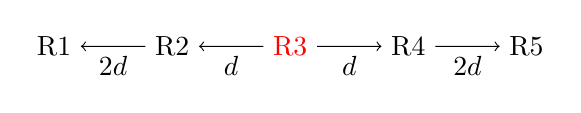
\begin{tikzpicture}[scale = 1.5]
\node (R1) at (.5, .5) {R1};
\node (R2) at (1.5,.5) {R2};
\node (R3) [color =  red]  at (2.5,.5) {R3};
\node (R4) at (3.5,.5) {R4};
\node (R5) at (4.5,.5) {R5};
\draw [->] (R3) -- (R2) node [midway, below] {$d$};
\draw [->] (R3) -- (R4) node [midway, below] {$d$};
\draw [->] (R2) -- (R1) node [midway, below] {$2d$};
\draw [->] (R4) -- (R5) node [midway, below] {$2d$};
\end{tikzpicture}
\end{figure}


When $\mW_n$ is an inverse distance matrix, its off-diagonal elements are defined as $w_{ij} = 1/d_{ij}$, where $d_{ij}$ represents the distance between two spatial units $i$ and $j$. The row sum of $\mW_n$ for any given $i$ is:
\begin{equation*}
  \sum_{j = 1}^n w_{ij} = 1/d + 1/d + 1/2d + 1/2d + \cdots = 2 \times (1/d + 1/2d + 1/3d + \cdots),  
\end{equation*}
%
which represents a harmonic series that diverges to infinity. 

This divergence is one of the main reasons why some empirical applications introduce a cutoff distance $d^*$, such that $w_{ij} = 0$ if $d_{ij} > d^*$. Imposing this cutoff ensures that the row sums remain finite and avoids potential numerical issues. 

However, note that even without a cutoff, the ratio of the row sum to the sample size,  
\begin{equation*}  
\frac{2 \times \left( \frac{1}{d} + \frac{1}{2d} + \frac{1}{3d} + \cdots \right)}{n},  
\end{equation*}  
converges to zero as $n \to \infty$. Therefore, the condition proposed by \cite{lee2004asymptotic} is satisfied, implying that an inverse distance matrix without a cutoff does not necessarily violate consistency requirements.  
Assumption \ref{assu:ml_3} excludes cases where the row sums, $\sum_{j=1}^n w_{ij}$ for $i = 1, \ldots, n$, diverge to infinity at a rate equal to or faster than the sample size $n$. In such cases, the maximum likelihood (ML) estimator would likely be inconsistent.  

A special case where the sequence $\{h_n\}$ is bounded arises when the number of neighbors is fixed, as in the $k$-nearest neighbors approach. However, the example of inverse distance weights highlights why these matrices can sometimes lead to numerical problems or unexpected outcomes in empirical applications. This is because, in practice, the sample size $n$ is typically finite and does not approach infinity, leading to potential complications with unbounded row sums.

%Assumptions~\ref{assu:ml_2} is always satisfied if $\left\lbrace h_n \right\rbrace$ is a bounded sequence. Think of $\mW_n$ as spatial weight matrix based on distances that is row-normalized. In this case the $i$th row

%\begin{equation*}
%  w_{i,n} = \frac{(d_{i1}, d_{i2}, ...,d_{in})}{\sum_{j = 1}^nd_{ij}}
%\end{equation*}

%where $d_{ij} > 0$ represents a function of the spatial distance of the $i$th and $j$th units in some space. For a row-normalized $\mW_n$, as $d_{i,j}$ are nonnegative constants and uniformly bounded, if the $\sum_{j = 1}^nd_{ij}, i = 1,...,n$ are uniformly bounded away from zero at the rate $h_n$ in the sense that $\sum_{j = 1}^nd_{ij} =O(h_n)$ uniformly in $i$ and $\lim \inf _{n\to \infty} h_n^{-1}\sum_{j = 1}^nd_{ij} > c$, where $c$ is a positive constant independent of $i$ and $n$, the implied normalized weights matrix will have the property of Assumption \ref{assu:ml_2}.

What happens if $h_n$ is unbounded? In this case $\sum_{j = 1}^nd_{ij}$ is uniformly bounded away from zero at the rate $h_n$, where $\lim_{n\to \infty}h_n = \infty$. This particular case \textbf{rules out} cases where each unit has only a fixed, finite number of neighbors, even as the total number of unit increases to infinity. For example, it excludes scenarios where spatial units correspond to counties, and neighbors are defined as those with contiguous border.

When does $h_n \to \infty$? This case requires that each unit in the limit has infinitely many neighbors. As noted by \cite{lee2002consistency}, in economic applications where (i) the neighbors of each unit are densely distributed in a relevant space, or (ii) each unit is significantly influenced by a large proportion of the total population units, it is likely that $\sum_{j=1}^n d_{ij}$ diverges and $(1/n)\sum_{j=1}^n d_{ij}$ converges as $n \to \infty$.   

For example, consider $d_{ij} = 1 / \left|r_i - r_j\right|$, where $r_i$ is the proportion of state $i$'s population of African descent. Since no state in the U.S. has a zero proportion of African-Americans, $d_{ij}> 0$. Here, $(1/n)\sum_{j = 1}^nd_{ij}$ will remain bounded away from zero, while $\sum_{j = 1}^nd_{ij}$ will diverge at a rate proportional to $n$.

Another case arises when all cross-sectional units are assumed to be neighbors of one another, with equal weights assigned. If all off-diagonal elements of the spatial weights matrix are $w_{ij} = 1$, then the row and column sums become $n - 1$, diverging to infinity as $n \to \infty$. However, in this scenario, $(n - 1)/n \to 1$ rather than converging to zero. Consequently, a spatial weight matrix with equal weights and subsequent row-normalization, $w_{ij} = 1/(n - 1)$, violates both \cite{lee2004asymptotic}'s and \cite{kelejian1998generalized, kelejian1999generalized}'s conditions, making it unsuitable for consistent estimation.  

Alternatively, a group interaction matrix, as introduced by Case (1991), satisfies the conditions. In this setup, ``neighbors'' refer to individuals within the same district. Suppose there are $R$ districts and $m$ individuals per district, with a total sample size $n = mR$. Each neighbor within a district is given equal weight, and the spatial weight matrix is defined as $\mW_n = \mI_R \otimes \mB_m$, where $\mB_m = (\vones_m \vones_m^\top - \mI_m)/(m - 1)$.  

Here, $h_n = m - 1$, and $h_n/n = (m - 1)/(mR) = O(1/R)$. If the sample size $n$ increases through growth in both $R$ and $m$, $h_n \to \infty$ and $h_n/n \to 0$ as $n \to \infty$. Thus, this matrix satisfies \cite{lee2004asymptotic}'s condition.  

\begin{remark}
  The boundedness or divergence of $\{h_n\}$ has significant implications for OLS estimation. When $\{h_n\}$ is bounded, the OLS estimators of $\vbeta$ and $\rho$ are inconsistent. However, when $\{h_n\}$ diverges, these estimators can be consistent \citep[see][]{lee2002consistency}. 
\end{remark}

In summary, when $\{h_n\}$ is a bounded sequence, it implies that each unit has a fixed, small number of neighbors, typically based on geographical proximity. In contrast, when $\{h_n\}$ diverges, it reflects scenarios where each unit interacts with a large number of neighbors, which frequently occurs in empirical studies of social networks, economic spillovers, or cluster sampling data.

%------------------------------------------------------------------------------------------------
\begin{assumption}[Non-singularity of $\mA_n$ \citep{lee2004asymptotic}]\label{assu:ml_4}
	The matrix $\mA_n$ is nonsingular.
\end{assumption}
%------------------------------------------------------------------------------------------------

Under Assumption \ref{assu:ml_4}, the SLM (system) has the reduced form (equilibrium) given by
\begin{equation*}
\vy_n = \mA^{-1}_{n0}(\mX_n\vbeta_0 + \vepsi_n),
\end{equation*}
%
where $\mA^{-1}_{n0} = (\mI_n - \rho_0\mW_n)$ and with the following expectation and variance:
\begin{eqnarray*}
\E(\vy_n)   &=& \left(\mI_n - \rho_0\mW_n\right)^{-1}\mX_n\vbeta  = \mA_{n0}^{-1}\mX_n\vbeta_0,\\
\var(\vy_n) &=& \E(\vy_n\vy_n^\top) = \sigma^2_{0}\left(\mI_n - \rho_0\mW_n\right)^{-1}\left[\left(\mI_n - \rho_0\mW_n\right)^{-1}\right]^\top = \sigma^2_0\mA_{n0}^{-1}(\mA_{n0}^{-1})^\top.
\end{eqnarray*}

For further reference, note that we can write the reduced-form equation as follows:
\begin{equation*}
	\begin{aligned}
	\vy_n & = \mX_n\vbeta_0 + \rho_0\mW_n\vy_n + \vepsi_n, \\
	      & = \mX_n\vbeta_0 + \rho_0\mW_n\left[\mA^{-1}_{n0}\mX_n\vbeta_0 + \mA^{-1}_{n0}\vepsi_n\right] + \vepsi_n, \\
	      & = \mX_n\vbeta_0 + \rho_0\mW_n\mA^{-1}_{n0}\mX_n\vbeta_0 + \rho_0\mW_n\mA^{-1}_{n0}\vepsi_n + \vepsi_n, \\
	      & = \mX_n\vbeta_0 + \rho_0\mW_n\mA^{-1}_{n0}\mX_n\vbeta_0  + \left(\mI_n + \rho_0\mW_n\mA^{-1}_{n0}\right)\vepsi_n, \\
	      & = \mX_n\vbeta_0 + \rho_0\mC_{n0}\mX_n\vbeta_0  + \left(\mI_n + \rho_0\mC_{n0}\right)\vepsi_n, \\
	      & = \mX_n\vbeta_0 + \rho_0\mC_{n0}\mX_n\vbeta_0  +\mA_{n0}^{-1}\vepsi_n,
	\end{aligned}
\end{equation*}
%
because $\mI_n + \rho_0\mC_n = \mA_{n0}^{-1}$ (see Exercise  \ref{lab:4.6}), where $\mC_{n0}=\mW_n\mA_{n0}^{-1}$. 

%-------------------------------------------------------------------------------------
\begin{assumption}[Uniform boundedness  \citep{lee2004asymptotic}]\label{assu:ml_5}
	The sequences of matrices $\left\lbrace \mW_n \right\rbrace$ and $\left\lbrace \mA_n^{-1} \right\rbrace$ are uniformly bounded in both row and column sums 
\end{assumption}
%-------------------------------------------------------------------------------------

The uniform boundedness of the matrices is a condition to limit the spatial correlation to a manageable degree. For example, it guarantees that the variances of $\vy_n$ are bounded as $n$ goes to infinity. See our discussion in Section \ref{sec:bounded-matrices}.

Why do we care about this? Because we need the variance goes to zero when the sample size goes to infinity in order to apply some consistency theorem.\footnote{Equivalently, this assumption rules out the unit root case in time series.}

%-------------------------------------------------------------------------------------

\begin{lemma}[Uniform Boundedness of Matrices in Row and Column Sums]
  Suppose that the spatial weights matrix $\mW_n$ is a non-negative matrix with its $(i,j)$th element being 
  \begin{equation*}
    w_{n,ij} = \frac{d_{ij}}{\sum_{l = 1}^nd_{il}}
  \end{equation*}
  %
  and $d_{ij}>0$ for all $i,j$.
  
  \begin{enumerate}
    \item If the row sums $\sum_{j = 1}^nd_{ij}$ are bounded away from zero at the rate $h_n$ uniformly in $i$, and the column sums $\sum_{i = 1}^nd_{ij}$ are $O(h_n)$ uniformly in $j$, then $\left\lbrace \mW_n \right\rbrace$  are uniformly bounded in column sums.
    \item (Symmetric Matrix) If $d_{ij} = d_{ji}$ for all $i$ and $j$ and the row sums $\sum_{j = 1}^nd_{ij}$ are $O(h_n)$ and bounded away from zero at the rate $h_n$ uniformly in $i$, then $\left\lbrace \mW_n \right\rbrace$  are uniformly bounded in column sums.
  \end{enumerate}
\end{lemma}
%-------------------------------------------------------------------------------------

%-------------------------------------------------------------------------------------

\begin{assumption}[No asymptotic multicollinearity \citep{lee2004asymptotic}]\label{assu:ml_6}
	The elements of $\mX_n$ are uniformly bounded constants for all $n$. The $\lim_{n\to \infty}\mX_n^\top\mX_n/n$ exists and is nonsingular. 
\end{assumption}
%-------------------------------------------------------------------------------------

This rules out multicollinearity among the regressors. Note also that we are assuming that $\mX_n$ is \textbf{nonstochastic}. If $\mX_n$ were stochastic, then we will require:
\begin{equation*}
  \plim_{n\to \infty}\mX_n^\top\mX_n/ n,
\end{equation*}
%
to exists.

%-------------------------------------------------------------------------------------

\begin{assumption}[Uniform Boundedness of ${\mA_n^{-1}(\rho)}$ \cite{lee2004asymptotic}]\label{assu:ml_7}
	${\mA_n^{-1}(\rho)}$ are uniformly bounded in either row or column sums, uniformly in $\rho$ in a compact parameter space $\Gamma$. The true parameter $\rho_0$ is in the interior of $\Gamma$
\end{assumption}
%-------------------------------------------------------------------------------------

This assumption is needed to deal with the nonlinearity of $\log \left|\left(\mI_n - \rho \mW\right)^{-1}\right|$ in the log-likelihood function. Recall that if $\left\| \rho\mW\right\| < 1$, then $\mI_n - \rho\mW_n$ is invertible for all $n$. Then if $\left\| \rho\mW\right\| < 1$, then the sequence of matrices $\left\|\left(\mI_n- \rho\mW_n\right)^{-1}\right\|$ are uniformly bounded in any subset of $(-1, 1)$ bounded away from the boundary. As we previously see, if $\mW_n$ is row-standardized $\left(\mI_n- \rho\mW\right)^{-1}$ is uniformly bounded in row sums norm uniformly in any closed subset of $(-1, 1)$. Therefore, $\Gamma$ from Assumption~\ref{assu:ml_7} can be considered as a single closed set contained in (-1, 1).

What if $\mW_n$ is not row-normalized but its eigenvalues are real? Then, the Jacobian of $\left|\left(\mI_n- \rho\mW\right)^{-1}\right|$ will be positive if $-1/\omega_{min} < \rho < 1/\omega_{max}$, where $\omega_{min}$ and $\omega_{max}$ are the minimum and maximum eigenvalues of $\mW_n$, and $\Gamma$ will be a closed interval contained in $(-1/\omega_{min}, 1/\omega_{max})$ for all $n$. Thus, Assumption~\ref{assu:ml_7} rules out models where $\rho_0$ is close to -1 and 1.  

%-------------------------------------------------------------------------------------
\begin{assumption}[Identification \citep{lee2004asymptotic}]\label{assu:ml_8}
		The
		\begin{equation*}
			\lim_{n\to \infty}\frac{1}{n}\left(\mX_n, \mC_n\mX_n\vbeta_0\right)'\left(\mX_n, \mC_n\mX_n\vbeta_0\right)
		\end{equation*}
		%
		 exists and is nonsingular.
\end{assumption}
%-------------------------------------------------------------------------------------

This is a sufficient condition for global identification of $\vtheta_0$.

%-------------------------------------------------------------------------------------
\begin{theorem}[Consistency]\label{teorem:Consistency_ML}
	Let $\vtheta_0 = (\vbeta_0^\top, \rho_0, \sigma_0^2)^\top$. Under assumption \ref{assu:ml_1}-\ref{assu:ml_8}, $\vtheta_0$ is globally identifiable and $\widehat{\vtheta}_n$ is a consistent estimator of $\vtheta_0$.
\end{theorem}
%-------------------------------------------------------------------------------------


Identification of $\rho_0$ can be based on the maximum values of the concentrated log-likelihood function $Q_n(\rho) / n$. With identification and uniform convergence of $\left[\log L_n(\rho) - Q_n(\rho)\right] / n$ to zero on $\Gamma$, consistency of the QMLE $\widehat{\vtheta}_n$ follows. The sketch of the proof for Theorem \ref{teorem:Consistency_ML} is given in Appendix \ref{appendix-consistency}. 

For a proof without compactness of the parameter space (proving concavity of the log-likelihood function) see \cite{liu2022consistency}.

%=====================================
\subsection{Asymptotic Normality}
%=====================================

To derive the asymptotic distribution of the QML and ML we need the asymptotic behavior of the gradient. Taking a Taylor series expansion around $\vtheta_0$ of $\partial \ell_n(\widehat{\vtheta}_n)/ \partial \vtheta = 0$ at $\vtheta_0$, we get
\begin{equation*}
  \frac{\partial \ell_n(\widehat{\vtheta}_n)}{\partial \vtheta} =  \frac{\partial \ell_n(\vtheta_0)}{\partial \vtheta} + \frac{\partial^2 \ell_n(\widetilde{\vtheta}_n)}{\partial \vtheta \partial \vtheta^\top}(\widehat{\vtheta}_n - \vtheta_0),
\end{equation*}
%
where $\widetilde{\vtheta}_n = \alpha_n \widehat{\vtheta}_n + (1 - \alpha_n)\vtheta_0$ and $\alpha_n\in \left[ 0, 1\right]$, therefore:
\begin{equation}\label{eq:sampling-error-ml}
  \sqrt{n}(\widehat{\vtheta}_n - \vtheta_0) = - \left[\frac{1}{n}\frac{\partial^2 \ell_n(\widetilde{\vtheta}_n)}{\partial \vtheta \partial \vtheta^\top}\right]^{-1}\frac{1}{\sqrt{n}}\frac{\partial \ell_n(\vtheta_0)}{\partial \vtheta}.
\end{equation}

As standard in asymptotic theory of MLE, we need to show that the first element of the rhs of \eqref{eq:sampling-error-ml} converges to some finite matrix. We also need to find the limiting distribution of $\frac{1}{\sqrt{n}}\frac{\partial \ell_n(\vtheta_0)}{\partial \vtheta}$. Recall that the first-order derivatives of the log-likelihood function \textbf{evaluated at $\vtheta_0$} are given by (see Section \ref{sec:score_sml}):
\begin{align}
	\frac{1}{\sqrt{n}}\frac{\partial \ell_n(\vtheta_0)}{\partial \vbeta} & = \frac{1}{\sigma^2_0\sqrt{n}}\mX_n^\top\vepsi_n \\
	\frac{1}{\sqrt{n}}\frac{\partial \ell_n(\vtheta_0)}{\partial \sigma^2} & = \frac{1}{2\sigma_0^4\sqrt{n}}\left(\vepsi_n'\vepsi_n - n\sigma_0^2\right) \\
		\frac{1}{\sqrt{n}}\frac{\partial \ell_n(\vtheta_0)}{\partial \rho} & = \frac{1}{\sigma_0^2\sqrt{n}}(\mC_{n0}\mX_n\vbeta_0)^\top \vepsi_n + \frac{1}{\sigma_0^2\sqrt{n}}(\vepsi_n^\top\mC_{n0}\vepsi_n - \sigma_0^2\tr(\mC_{n0}))\label{eq:asy_der_rho}
\end{align}	

As explained by \citet[][pag. 1905]{lee2004asymptotic}, these are linear and quadratic functions of $\vepsi_n$. In particular, the asymptotic distribution of \eqref{eq:asy_der_rho} may be derived from central limit theorem for linear-quadratic forms. The matrix $\mC_{n0}$ is uniformly bounded in row sums. As the elements of $\mX_n$ are bounded, the elements of $\mC_{n0}\mX_n\vbeta_0$ for all $n$ are uniformly bounded by Lemma \ref{lemma:bounded_lemma}. With the existence of high order moments of $\epsilon$ in Assumption \ref{assu:ml_1}, the central limit theorem for quadratic forms of double arrays of \cite{kelejian2001asymptotic} can be applied and the limit distribution of the score vector follows.

Let $\vtheta = (\vbeta^\top, \rho, \sigma^2)^\top$ be the $k+2$-dimensional vector. Since $\E\left[(1 / \sqrt{n}) \partial \ell_n (\vtheta_0)/\partial \vtheta\right]  = \vzeros$,  the variance matrix of $(1 / \sqrt{n}) \partial \ell_n(\vtheta_0) /\partial \vtheta$ is:
\begin{equation*}
  \E\left[\frac{1}{\sqrt{n}}\frac{\partial \ell_n (\vtheta_0)}{\partial \vtheta}\cdot\frac{1}{\sqrt{n}}\frac{\partial \ell_n (\vtheta_0)}{\partial \vtheta^\top} \right] = - \E\left(\frac{1}{n} \frac{\partial \ell_n(\vtheta_0)}{\partial \vtheta \partial \vtheta^\top}\right) + \mOmega_{\vtheta, n},
\end{equation*}
%
where 
\begin{equation}\label{eq:expected-hessian-slm-asy}
- \E\left(\frac{1}{n} \frac{\partial^2 \ell_n(\vtheta_0)}{\partial \vtheta \partial \vtheta^\top}\right)= 
	\begin{pmatrix}
	\frac{1}{n\sigma^2_0}(\mX_n^\top \mX_n)  & \frac{1}{n\sigma^2_0} \mX_n^\top (\mC_n\mX_n\vbeta_0) & \vzeros^\top \\
	   & \frac{1}{n}\tr(\mC^s_{n0}\mC_{n0}) + \frac{1}{n\sigma^2_0}(\mC_{n0}\mX_n\vbeta_0)^\top(\mC_{n0}\mX_n\vbeta_0) &  \frac{1}{n\sigma^2_0} \tr(\mC_{n0}) \\
		 &  & \frac{1}{2\sigma^4_0}
	\end{pmatrix} 
\end{equation}
%
and $\mC^s_{n0} = \mC_{n0} + \mC_{n0}^\top$. Equation \eqref{eq:expected-hessian-slm-asy} represents the average Hessian matrix (or information matrix when $\vepsi$'s are \textbf{normal}). The matrix $ \mOmega_{\vtheta, n}$ is 
\begin{equation}\label{eq:Omega-slm-ml}
\mOmega_{\vtheta, n}  = \begin{pmatrix} 
                            \vzeros & * & * \\
                            \frac{\mu_{3}}{n\sigma_0^4}\sum_{i = 1}^n\mC_{n, ii}\vx_{i, n} & \frac{2\mu_3}{n\sigma_0^4}\sum_{i = 1}^n\mC_{n, ii}\mC_{n, ii}\mX_m\vbeta_0 + \frac{(\mu_4 - 3\sigma_0^4)}{n\sigma_0^4}\sum_{i = 1}^n\mC_{n, ii}^2 & * \\
                            \frac{1}{n2\sigma_0^6}\left[\mu_3\vones_n^\top\mG_n\mX_n\vbeta_0 + (\mu_4 -3\sigma_0^4)\tr(\mG_n)\right] & \frac{(\mu - 3\sigma_0^4)}{4\sigma_0^8}
                         \end{pmatrix}
\end{equation}
%
which is a symmetric matrix with the second, third, and fourth moments of $\vepsi$. If $\vepsi_n$ is normally distributed, then $\mOmega_{\vtheta, n} = \mZeros$. 

Derivation of \eqref{eq:expected-hessian-slm-asy} is given in Appendix \ref{appendix-EH-sml} and the variance of the score function is given in Appendix \ref{appendix-score}.


%---------------------------------------------------
\begin{theorem}[Asymptotic Normality]\label{teo:asymptotic-normality-slm}
Under Assumptions \ref{assu:ml_1}-\ref{assu:ml_8}, 
\begin{equation}
  \sqrt{n}\left(\widehat{\vtheta}_n- \vtheta_0\right)\dto \rN\left(\vtheta, \mSigma_{\vtheta}^{-1} + \mSigma_{\vtheta}^{-1}\mOmega_{\vtheta}\mSigma_{\vtheta}^{-1}\right),
\end{equation}
%
where $\mOmega_{\vtheta} = \lim_{n\to\infty}\mOmega_{\vtheta, n}$ and
\begin{equation}
  \mSigma_{\vtheta}= - \lim_{n\to\infty} \E\left[\frac{1}{n}\frac{\partial^2 \log L_n(\vtheta_0)}{\partial \vtheta \partial \vtheta^\top}\right],
\end{equation}
which are assumed to exists. If the $\epsilon_i$'s are \textbf{normally distributed}, then:
\begin{equation}
  \sqrt{n}\left(\widehat{\vtheta}_n- \vtheta_0\right)\dto \rN\left(\vtheta, \mSigma_{\vtheta}^{-1}\right).
\end{equation}
\end{theorem}
%-------------------------------------

A sketch of the proof of Theorem \ref{teo:asymptotic-normality-slm} is given in Appendix \ref{appendix-asymptotic normality}.

%=====================================
\section{Computing the Standard Errors For The Marginal Effects}
%=====================================

In section \ref{sec:summary-measures}, we explain how to obtain summary measures for the direct, indirect and total effects. However, we did not explain how to obtain standard errors for such measures. For example, we would like to have confidence intervals for the indirect effects and to be able to say whether they are significant. 

Recall that our three summary measures are:
\begin{eqnarray*}
\bar{M}(\vtheta)_{\mbox{direct}} & = & n^{-1}\tr\left[\mS_r(\vtheta)\right], \\
\bar{M}(\vtheta)_{\mbox{total}} & = & n^{-1}\vones_n^\top\mS_r(\vtheta)\vones_n, \\
\bar{M}(\vtheta)_{\mbox{indirect}} & = & \bar{M}(r)_{\mbox{total}} - \bar{M}(r)_{\mbox{direct}},
\end{eqnarray*}
%
which are highly nonlinear due to $\mS_r(\vtheta)$.\footnote{Note that we have replaced the parameter for the spatially lagged independent variable to let $\vtheta$ be the vector parameters of the model. } Therefore, a procedure such as the Delta Method is difficult to perform. Instead, we can use a Monte Carlo approximation which takes into account the sampling distribution of $\vtheta$. To show this procedure, consider the SDM where:
\begin{equation*}
\mS(\vtheta)_r = \left(\mI_n - \rho\mW\right)^{-1}\left(\mI_n\beta_r + \mW\gamma_r\right).
\end{equation*}

Let $g(\vtheta)= \bar{M}(\vtheta)$ be a function representing the marginal (direct, indirect or total) effect that depends on the population parameters $\vtheta$. If $\rN(\vtheta|\bar{\vtheta}, \mSigma_{\theta})$ denotes the multivariate normal density of $\vtheta$ with mean $\bar{\vtheta}$ and asymptotic variance-covariance matrix $\mSigma_{\theta}$, then the expected value of the marginal effects conditional on the population parameters $\bar{\vtheta}$ and $\mSigma_{\theta}$ is:
\begin{equation*}
\E\left[g(\vtheta)|\bar{\vtheta}, \mSigma_{\theta}\right] = \int_{\vtheta}\E\left[g(\vtheta)|\vy, \mX, \vtheta\right]\rN(\vtheta|\bar{\vtheta}, \mSigma_{\theta})d\vtheta. 
\end{equation*}

A Monte Carlo approximation to this expectation is obtained by calculation of the empirical marginal effects evaluated at pseudo draws of $\vtheta$ from the asymptotic distribution of the estimator. The algorithm is the following:

%------------------------------------------------------------------
\begin{algorithm}[Standard Errors of the Marginal Effects]
Estimate the model using MLE. Consider $s = 1, \ldots, S$, and start with $s = 1$
\begin{enumerate}
  \item Take a random draw of $\vtheta^{s}$ from $\rN(\widehat{\bar{\vtheta}}, \widehat{\mSigma}_{\theta})$, which is the estimated asymptotic distribution of $\widehat{\vtheta}$. 
 \item Compute the marginal effect, but substituting  $\widehat{\vtheta}$ for $\vtheta^s$. 
 \item Update $s = s + 1$, and go back to step 1. 
 \item Repeat for a large number of repetitions S (e.g., S = 1000).  
 \item Calculate the empirical mean of the marginal effects. The standard error of the marginal effect across the $S$ draws is the standard error. 
\end{enumerate}
\end{algorithm}
%------------------------------------------------------------------

%====================================
\section{Spillover Effects on Crime: An Application in R}\label{sec:Anselin-example}
%====================================


\subsection{Estimation of Spatial Models in R}

This example uses the dataset from \citet{anselin1988spatial}, which provides a cross-sectional view of 49 neighborhoods in Columbus, Ohio. The goal is to explain the crime rate as a function of household income and housing values. The dataset includes the following variables:

\begin{itemize}
  \item \texttt{CRIME}: residential burglaries and vehicle thefts per thousand household in the neighborhood.
  \item \texttt{HOVAL}: housing value in US\$1,000.
  \item \texttt{INC}: household income in US\$1,000.
\end{itemize}

We begin the analysis by loading the necessary \proglang{R} packages into the workspace:

\begin{knitrout}
\definecolor{shadecolor}{rgb}{0.969, 0.969, 0.969}\color{fgcolor}\begin{kframe}
\begin{alltt}
\hlcom{# Load packages}
\hlkwd{library}\hldef{(}\hlsng{"spdep"}\hldef{)}
\hlkwd{library}\hldef{(}\hlsng{"tmap"}\hldef{)}
\hlkwd{library}\hldef{(}\hlsng{"spatialreg"}\hldef{)}
\hlkwd{library}\hldef{(}\hlsng{"memisc"}\hldef{)}            \hlcom{# Package for tables}
\hlkwd{library}\hldef{(}\hlsng{"RColorBrewer"}\hldef{)}
\hlkwd{library}\hldef{(}\hlsng{"classInt"}\hldef{)}
\hlkwd{source}\hldef{(}\hlsng{"getSummary.sarlm.R"}\hldef{)} \hlcom{# Function for spdep models}
\end{alltt}
\end{kframe}
\end{knitrout}

The dataset is available in the \pkg{spdep} package, and we load it as follows:

\begin{knitrout}
\definecolor{shadecolor}{rgb}{0.969, 0.969, 0.969}\color{fgcolor}\begin{kframe}
\begin{alltt}
\hlcom{# Load data}
\hldef{columbus} \hlkwb{<-} \hlkwd{st_read}\hldef{(}\hlkwd{system.file}\hldef{(}\hlsng{"shapes/columbus.gpkg"}\hldef{,} \hlkwc{package}\hldef{=}\hlsng{"spData"}\hldef{)[}\hlnum{1}\hldef{],}
                           \hlkwc{quiet} \hldef{=} \hlnum{TRUE}\hldef{)}
\hldef{col.gal.nb} \hlkwb{<-} \hlkwd{poly2nb}\hldef{(columbus)}
\end{alltt}
\end{kframe}
\end{knitrout}

Before estimating models, it is essential to determine whether there is a spatial pattern in the crime variable. To visualize this, we create a choropleth map for \texttt{CRIME}:

\begin{knitrout}
\definecolor{shadecolor}{rgb}{0.969, 0.969, 0.969}\color{fgcolor}\begin{kframe}
\begin{alltt}
\hlcom{# Spatial distribution of crime}
\hlkwd{tm_shape}\hldef{(columbus)} \hlopt{+}
  \hlkwd{tm_polygons}\hldef{(}\hlsng{"CRIME"}\hldef{,}
              \hlkwc{title} \hldef{=} \hlsng{"Crime Status"}\hldef{,}
              \hlkwc{parlette} \hldef{=} \hlsng{"RdYBu"}
              \hldef{)} \hlopt{+}
  \hlkwd{tm_layout}\hldef{(}\hlkwc{frame} \hldef{=} \hlnum{FALSE}\hldef{)}
\end{alltt}
\end{kframe}
\end{knitrout}

The map in Figure~\ref{fig:spatial-crime} suggests a positive spatial autocorrelation in crime rates. To confirm this, we perform Moran's I test using a row-normalized binary contiguity matrix, \texttt{col.gal.nb}, based on the Queen criterion. The Moran test is performed using Monte Carlo simulations with 99 replications:

\begin{figure}[ht]
\caption{Spatial Distribution of Crime in Columbus, Ohio Neighborhoods}
    \label{fig:spatial-crime}
    \centering 
	\begin{minipage}{.9\linewidth}
\begin{knitrout}
\definecolor{shadecolor}{rgb}{0.969, 0.969, 0.969}\color{fgcolor}

{\centering \includegraphics[width=9cm,height=9cm]{figure/spatial-crime-1} 

}


\end{knitrout}
\footnotesize
		\emph{Notes:} This graph shows the spatial distribution of crime on the 49 Columbus, Ohio neighborhoods. Darker color indicates greater rate of crime. 
	\end{minipage}	
\end{figure}


\begin{knitrout}
\definecolor{shadecolor}{rgb}{0.969, 0.969, 0.969}\color{fgcolor}\begin{kframe}
\begin{alltt}
\hlcom{# Moran's I test}
\hlkwd{set.seed}\hldef{(}\hlnum{1234}\hldef{)}
\hldef{listw} \hlkwb{<-} \hlkwd{nb2listw}\hldef{(col.gal.nb,} \hlkwc{style} \hldef{=} \hlsng{"W"}\hldef{)}
\hlkwd{moran.mc}\hldef{(columbus}\hlopt{$}\hldef{CRIME,} \hlkwc{listw} \hldef{= listw,}
           \hlkwc{nsim} \hldef{=} \hlnum{99}\hldef{,} \hlkwc{alternative} \hldef{=} \hlsng{'greater'}\hldef{)}
\end{alltt}
\begin{verbatim}
## 
## 	Monte-Carlo simulation of Moran I
## 
## data:  columbus$CRIME 
## weights: listw  
## number of simulations + 1: 100 
## 
## statistic = 0.50019, observed rank = 100, p-value = 0.01
## alternative hypothesis: greater
\end{verbatim}
\end{kframe}
\end{knitrout}

The Moran's I statistic is 0.51 with a p-value of 0.01, providing evidence of positive spatial autocorrelation. This indicates that neighborhoods with high (low) crime rates tend to be surrounded by neighborhoods with similarly high (low) crime rates. 

Next, we estimate various spatial models using functions from the \pkg{spatialreg} package. These models include:

\begin{itemize} 
\item \textbf{OLS}: Estimated using the \texttt{lm} function. 
\item \textbf{SLX}: Estimated with the \texttt{lm} function, using the \texttt{lag.listw} function from \pkg{spdep} to create $\mW\mX$. Alternatively, the \texttt{lmSLX} function from \pkg{spatialreg} can be used. \item \textbf{SLM}: Estimated using the \texttt{lagsarlm} function from \pkg{spatialreg}. 
\item \textbf{SDM}: Estimated with \texttt{lagsarlm} using the \texttt{type = "mixed"} argument. Alternatively, \texttt{type = "Durbin"} may be specified. 
\item \textbf{SEM}: Estimated using the \texttt{errorsarlm} function. The Spatial Durbin Error Model (SDEM) can be estimated with \texttt{type = "emixed"}. 
\item \textbf{SAC}: Estimated with the \texttt{sacsarlm} function. 
\end{itemize}

These models are estimated using Maximum Likelihood (ML) methods, as outlined in the previous section. To compute the determinant of the Jacobian, we follow the approach of \citet{ord1975estimation} and explicitly set \texttt{method = "eigen"} in the spatial model functions, ensuring consistency with Equation~\eqref{eq:Ord-determinant}.
\begin{knitrout}
\definecolor{shadecolor}{rgb}{0.969, 0.969, 0.969}\color{fgcolor}\begin{kframe}
\begin{alltt}
\hlcom{# Models}
\hldef{columbus}\hlopt{$}\hldef{lag.INC}   \hlkwb{<-} \hlkwd{lag.listw}\hldef{(listw,}
                         \hldef{columbus}\hlopt{$}\hldef{INC)}   \hlcom{# Create spatial lag of INC}
\hldef{columbus}\hlopt{$}\hldef{lag.HOVAL} \hlkwb{<-} \hlkwd{lag.listw}\hldef{(listw,}
                         \hldef{columbus}\hlopt{$}\hldef{HOVAL)} \hlcom{# Create spatial lag of HOVAL}
\hldef{ols} \hlkwb{<-} \hlkwd{lm}\hldef{(CRIME} \hlopt{~} \hldef{INC} \hlopt{+} \hldef{HOVAL,}
          \hlkwc{data} \hldef{=  columbus)}
\hldef{slx} \hlkwb{<-} \hlkwd{lm}\hldef{(CRIME} \hlopt{~} \hldef{INC} \hlopt{+} \hldef{HOVAL} \hlopt{+} \hldef{lag.INC} \hlopt{+} \hldef{lag.HOVAL,}
          \hlkwc{data} \hldef{=  columbus)}
\hldef{slm} \hlkwb{<-} \hlkwd{lagsarlm}\hldef{(CRIME} \hlopt{~} \hldef{INC} \hlopt{+} \hldef{HOVAL,}
                \hlkwc{data} \hldef{= columbus,}
                \hldef{listw,}
                \hlkwc{method} \hldef{=} \hlsng{"eigen"}\hldef{)}
\hldef{sdm} \hlkwb{<-} \hlkwd{lagsarlm}\hldef{(CRIME} \hlopt{~} \hldef{INC} \hlopt{+} \hldef{HOVAL,}
                \hlkwc{data} \hldef{= columbus,}
                \hldef{listw,}
                \hlkwc{method} \hldef{=} \hlsng{"eigen"}\hldef{,}
                \hlkwc{type} \hldef{=} \hlsng{"mixed"}\hldef{)}
\hldef{sem} \hlkwb{<-} \hlkwd{errorsarlm}\hldef{(CRIME} \hlopt{~} \hldef{INC} \hlopt{+} \hldef{HOVAL,}
                \hlkwc{data} \hldef{= columbus,}
                \hldef{listw,}
                \hlkwc{method} \hldef{=} \hlsng{"eigen"}\hldef{)}
\hldef{sac} \hlkwb{<-} \hlkwd{sacsarlm}\hldef{(CRIME} \hlopt{~} \hldef{INC} \hlopt{+} \hldef{HOVAL,}
                \hlkwc{data} \hldef{= columbus,}
                \hldef{listw,}
                \hlkwc{method} \hldef{=} \hlsng{"eigen"}\hldef{)}
\end{alltt}
\end{kframe}
\end{knitrout}

Note that the SLX model can also be estimated as follows:

\begin{knitrout}
\definecolor{shadecolor}{rgb}{0.969, 0.969, 0.969}\color{fgcolor}\begin{kframe}
\begin{alltt}
\hldef{slx2} \hlkwb{<-} \hlkwd{lmSLX}\hldef{(CRIME} \hlopt{~} \hldef{INC} \hlopt{+} \hldef{HOVAL,}
              \hlkwc{data} \hldef{= columbus,}
              \hldef{listw)}
\hlkwd{summary}\hldef{(slx2)}
\end{alltt}
\end{kframe}
\end{knitrout}


The results of the estimations are presented in Table \ref{tab:columbus-models}. Column 1 reports the OLS estimates. The findings suggest that, on average, an increase of one thousand dollars in neighborhood income is associated with a reduction of 1.6 crimes per thousand households. Similarly, an increase of one thousand dollars in housing value is associated with a reduction of 0.3 crimes per thousand households. Both coefficients are statistically significant.\footnote{We use the term "associated" because potential endogeneity issues in either variable could affect causal interpretation.} These results imply that residential burglaries and vehicle thefts are less prevalent in wealthier neighborhoods.

Column 2 shows the results for the SLX model, specified as 
\[
\vy = \mX\vbeta + \mW\mX\vgamma + \vepsi,
\]
where \(\mW\mX\) is a \(49 \times 2\) matrix representing the spatial lags of \texttt{INC} and \texttt{HOVAL}. The coefficient for the spatial lag of income (\texttt{W.INC}) is negative and statistically significant, indicating that crime in a given neighborhood is inversely related to the income levels of its neighboring areas. This suggests that higher income among neighbors is associated with lower crime levels in the focal neighborhood. Conversely, the coefficient for the spatial lag of housing value (\texttt{W.HOVAL}) is positive but not statistically significant, implying no clear relationship between the housing values of neighboring areas and crime.

Column 3 presents the results for the Spatial Lag Model (SLM). The spatial autoregressive parameter \(\rho\) is positive and significant, providing strong evidence of spatial autocorrelation and spillover effects in crime. The coefficients for the explanatory variables are qualitatively similar to the OLS results, though smaller in absolute magnitude, reflecting the influence of incorporating spatial dependence.

The Spatial Durbin Model (SDM) results are reported in column 4. The estimated \(\rho\) parameter remains positive and significant, confirming the presence of endogenous spatial interaction effects. However, the coefficients for the spatially lagged explanatory variables are not statistically significant. This suggests that once endogenous interaction effects in crime are accounted for, the socio-economic characteristics of neighboring areas do not significantly influence crime in the focal neighborhood. Furthermore, the coefficient for the spatial lag of income exhibits an unexpected positive sign, which contradicts the common factor hypothesis. This discrepancy suggests that the primary spatial effect may stem from an omitted spatial lag variable rather than spatial dependence in the error term.

Column 5 contains the results for the Spatial Error Model (SEM). The autoregressive parameter for \(\mW\vu\) is positive and significant, indicating substantial spatial transmission of random shocks. This finding may reflect the omission of spatially correlated variables, which contributes to the propagation of unobserved shocks across neighboring areas.

Finally, the Spatial Autoregressive Combined (SAC) model results are shown in column 6. This model accounts for both endogenous interaction effects and interactions among error terms. The coefficients for \(\mW\vy\) and \(\mW\vu\) are not statistically significant when estimated jointly. However, when these interaction effects are separated, both coefficients become significant. This suggests that the SAC model may be overparameterized, leading to reduced statistical power and diminished significance levels for all variables.


\begin{table}[ht]
\caption{Spatial Models for Crime in Columbus, Ohio Neighborhoods.}\label{tab:columbus-models}
\centering
\begin{tabular}{lD{.}{.}{3}D{.}{.}{3}D{.}{.}{3}D{.}{.}{3}D{.}{.}{3}D{.}{.}{3}}
\toprule
 & 
\multicolumn{1}{c}{OLS} & 
\multicolumn{1}{c}{SLX} & 
\multicolumn{1}{c}{SLM} & 
\multicolumn{1}{c}{SDM} & 
\multicolumn{1}{c}{SEM} & 
\multicolumn{1}{c}{SAC}\\
\midrule
\emph{Constant} & 68.619^{***} & 74.553^{***} & 45.603^{***} & 44.320^{***} & 60.279^{***} & 47.915^{***}\\
                 & (4.735) & (6.716) & (7.257) & (13.045) & (5.366) & (9.986)\\
INC              & -1.597^{***} & -1.097^{**} & -1.049^{***} & -0.920^{**} & -0.957^{**} & -1.043^{**}\\
                 & (0.334) & (0.374) & (0.307) & (0.335) & (0.334) & (0.329)\\
HOVAL            & -0.274^{*} & -0.294^{**} & -0.266^{**} & -0.297^{**} & -0.305^{***} & -0.280^{**}\\
                 & (0.103) & (0.102) & (0.089) & (0.090) & (0.092) & (0.091)\\
$W.INC$          &  & -1.399^{*} &  & -0.584 &  & \\
                 &  & (0.560) &  & (0.574) &  & \\
$W.HOVAL$        &  & 0.215 &  & 0.258 &  & \\
                 &  & (0.208) &  & (0.187) &  & \\
$\rho$          &  &  & 0.423^{***} & 0.403^{*} &  & 0.369\\
                 &  &  & (0.120) & (0.161) &  & (0.196)\\
$\lambda$       &  &  &  &  & 0.547^{***} & 0.146\\
                 &  &  &  &  & (0.138) & (0.301)\\
\midrule
AIC              & 382.754 & 379.941 & 375.348 & 377.279 & 377.499 & 377.110\\
N                &  49     &  49     &  49     &  49     &  49     &  49    \\
\bottomrule
\multicolumn{7}{p{.7\linewidth}}{Significance: 
              $*** \equiv p < 0{.}001$; 
              $** \equiv p < 0{.}01$; 
              $* \equiv p < 0{.}05$}\\
\end{tabular}

\end{table}

%---------------------------------------------------
\subsection{Estimation of Marginal Effects in R}
%---------------------------------------------------

In this section, we extend the analysis from Section \ref{sec:lesage-example} by integrating the estimation of marginal effects using a real-world application in \proglang{R}. 

We begin by addressing the following question: What would happen to crime rates across all regions if income increased from 13.906 to 14.906 in the 30th region ($\Delta\texttt{INC} = 1$)? This is analogous to the question posed in the commuting-time example in the previous chapter. Following the approach in Section \ref{sec:lesage-example}, we use the reduced-form predictor defined by the formula:
\begin{equation*}
\widehat{\vy} = \E(\vy| \mX, \mW) = (\mI_n - \widehat{\rho}\mW)^{-1}\mX\widehat{\vbeta},
\end{equation*}
% 
to estimate the predicted values before and after the change in the income variable. Using the observed values of the exogenous variables and the reduced-form predictor, we compute the predicted values for \code{CRIME}, denoted as $\widehat{\vy}^1$, based on the previously estimated SLM model.

\begin{knitrout}
\definecolor{shadecolor}{rgb}{0.969, 0.969, 0.969}\color{fgcolor}\begin{kframe}
\begin{alltt}
\hlcom{# The predicted values}
\hldef{rho}       \hlkwb{<-} \hldef{slm}\hlopt{$}\hldef{rho}                                \hlcom{# Estimated rho from SLM model}
\hldef{beta_hat}  \hlkwb{<-} \hlkwd{coef}\hldef{(slm)[}\hlopt{-}\hlnum{1}\hldef{]}                          \hlcom{# Estimated parameters}
\hldef{A}         \hlkwb{<-} \hlkwd{invIrW}\hldef{(listw,} \hlkwc{rho} \hldef{= rho)}               \hlcom{# (I - rho*W)^\{-1\}}
\hldef{X}         \hlkwb{<-} \hlkwd{cbind}\hldef{(}\hlnum{1}\hldef{, columbus}\hlopt{$}\hldef{INC, columbus}\hlopt{$}\hldef{HOVAL)} \hlcom{# Matrix of observed variables}
\hldef{y_hat_pre} \hlkwb{<-} \hldef{A} \hlopt \hlkwd{crossprod}\hldef{(}\hlkwd{t}\hldef{(X), beta_hat)}        \hlcom{# y hat}
\end{alltt}
\end{kframe}
\end{knitrout}

Next, we increase \code{INC} by 1 in spatial unit 30 and calculate the reduced-form predictions, $\widehat{\vy}^2$, as follows:

\begin{knitrout}
\definecolor{shadecolor}{rgb}{0.969, 0.969, 0.969}\color{fgcolor}\begin{kframe}
\begin{alltt}
\hlcom{# The post-predicted values}
\hldef{col_new} \hlkwb{<-} \hldef{columbus} \hlcom{# copy the data frame}

\hlcom{# Change the income value}
\hldef{col_new[}\hlnum{30}\hldef{,} \hlsng{"INC"}\hldef{]} \hlkwb{<-} \hlnum{14.906}

\hlcom{# The predicted values}
\hldef{X_d}        \hlkwb{<-} \hlkwd{cbind}\hldef{(}\hlnum{1}\hldef{, col_new}\hlopt{$}\hldef{INC, col_new}\hlopt{$}\hldef{HOVAL)}
\hldef{y_hat_post} \hlkwb{<-} \hldef{A} \hlopt \hlkwd{crossprod}\hldef{(}\hlkwd{t}\hldef{(X_d), beta_hat)}
\end{alltt}
\end{kframe}
\end{knitrout}

Finally,  we compute the difference between pre- and post-predictions: $\widehat{\vy}^2 - \widehat{\vy}^1$:
\begin{knitrout}
\definecolor{shadecolor}{rgb}{0.969, 0.969, 0.969}\color{fgcolor}\begin{kframe}
\begin{alltt}
\hlcom{# The difference}
\hldef{delta_y}         \hlkwb{<-} \hldef{y_hat_post} \hlopt{-} \hldef{y_hat_pre}
\hldef{col_new}\hlopt{$}\hldef{delta_y} \hlkwb{<-} \hldef{delta_y}

\hlcom{# Show the effects}
\hlkwd{summary}\hldef{(delta_y)}
\end{alltt}
\begin{verbatim}
##        V1            
##  Min.   :-1.091e+00  
##  1st Qu.:-1.047e-02  
##  Median :-2.383e-03  
##  Mean   :-3.572e-02  
##  3rd Qu.:-4.923e-04  
##  Max.   :-5.038e-05
\end{verbatim}
\begin{alltt}
\hlkwd{sum}\hldef{(delta_y)}
\end{alltt}
\begin{verbatim}
## [1] -1.750446
\end{verbatim}
\end{kframe}
\end{knitrout}

According to the results from \code{sum(delta\_y)}, the predicted effect of this income increase is a decrease of 1.65 crimes per thousand households, accounting for both direct and indirect effects. In other words, increasing income by \$1,000 in region 30 leads to a system-wide adjustment, resulting in a new equilibrium where total crime decreases by approximately 1.7 crimes per thousand households.

Sometimes it is useful to visualize these effects. For instance, we might want to identify regions with high and low impacts due to the increase in \code{INC}. Let us define ``highly impacted regions'' as those where the crime rate decreases by more than 0.05. The following code generates Figure \ref{fig:predicted-effect}, which illustrates these regions:

\begin{knitrout}
\definecolor{shadecolor}{rgb}{0.969, 0.969, 0.969}\color{fgcolor}\begin{kframe}
\begin{alltt}
\hlkwd{tm_shape}\hldef{(col_new)} \hlopt{+}
  \hlkwd{tm_polygons}\hldef{(}\hlkwc{col} \hldef{=} \hlsng{"delta_y"}\hldef{,}
              \hlkwc{title} \hldef{=} \hlsng{"Impact"}\hldef{,}
              \hlkwc{breaks} \hldef{=} \hlkwd{c}\hldef{(}\hlopt{-}\hlnum{Inf}\hldef{,}\hlopt{-}\hlnum{0.05}\hldef{,} \hlnum{Inf}\hldef{),}
              \hlkwc{palette} \hldef{=} \hlkwd{c}\hldef{(}\hlsng{"red"}\hldef{,} \hlsng{"blue"}\hldef{)}
              \hldef{)} \hlopt{+}
  \hlkwd{tm_layout}\hldef{(}\hlkwc{frame} \hldef{=} \hlnum{FALSE}\hldef{)}
\end{alltt}
\end{kframe}
\end{knitrout}


\begin{figure}[ht]
  \caption{Effects of a Change in Region 30: Categorization}
    \label{fig:predicted-effect}
    \centering 
	\begin{minipage}{.9\linewidth}
\begin{knitrout}
\definecolor{shadecolor}{rgb}{0.969, 0.969, 0.969}\color{fgcolor}

{\centering \includegraphics[width=10cm,height=10cm]{figure/predicted-effect-1} 

}


\end{knitrout}
\footnotesize
		\emph{Notes:} This graph shows those regions that had low and high impact due to increase in \code{INC} in 30th. Red-colored regions are those regions with a decrease of crime rate larger than 0.05, whereas blue-colored regions are those regions with lower decrease of crime rate. 
	\end{minipage}	
\end{figure}

Now, we map the magnitude of the changes caused by altering \texttt{INC} in region 30. The following code produces the map, with the resulting visualization shown in Figure \ref{fig:predicted-effect2}.

\begin{knitrout}
\definecolor{shadecolor}{rgb}{0.969, 0.969, 0.969}\color{fgcolor}\begin{kframe}
\begin{alltt}
\hlcom{# Plot the magnitude of the ME}
\hldef{pal5}    \hlkwb{<-} \hlkwd{brewer.pal}\hldef{(}\hlnum{6}\hldef{,} \hlsng{"Spectral"}\hldef{)}
\hldef{cats5}   \hlkwb{<-} \hlkwd{classIntervals}\hldef{(col_new}\hlopt{$}\hldef{delta_y,} \hlkwc{n} \hldef{=} \hlnum{5}\hldef{,} \hlkwc{style} \hldef{=} \hlsng{"jenks"}\hldef{)}
\hldef{colors5} \hlkwb{<-} \hlkwd{findColours}\hldef{(cats5, pal5)}
\hlkwd{plot}\hldef{(col_new,} \hlkwc{col} \hldef{= colors5)}
\hlkwd{legend}\hldef{(}\hlsng{"topleft"}\hldef{,} \hlkwc{legend} \hldef{=} \hlkwd{round}\hldef{(cats5}\hlopt{$}\hldef{brks,} \hlnum{2}\hldef{),} \hlkwc{fill} \hldef{= pal5,} \hlkwc{bty} \hldef{=} \hlsng{"n"}\hldef{)}
\end{alltt}
\end{kframe}
\end{knitrout}

\begin{figure}[ht]
  \caption{Effects of a Change in Region 30: Magnitude}
    \label{fig:predicted-effect2}
        \centering 
	\begin{minipage}{.9\linewidth}
\begin{knitrout}
\definecolor{shadecolor}{rgb}{0.969, 0.969, 0.969}\color{fgcolor}

{\centering \includegraphics[width=10cm,height=10cm]{figure/predicted-effect2-1} 

}


\end{knitrout}
\footnotesize
		\emph{Notes:} This graph shows the spatial distribution of the changes caused by altering \texttt{INC} in region 30.
	\end{minipage}
\end{figure}


Next, we use the \code{impacts()} function from the \pkg{spatialreg} package to decompose the total effects of a unit change in each predictor variable into direct (local) effects, indirect (spillover) effects, and total effects. The \code{impacts()} function computes these measures using the reduced-form representation:
\begin{equation*}
  \begin{aligned}
    \vy & = \sum_{r = 1}^K \mA(\mW)^{-1}(\mI_n\beta_r) + \mA(\mW)^{-1}\vepsi \\
     \mA(\mW)^{-1} & = \mI_n + \rho\mW + \rho^2\mW^2 + \ldots
  \end{aligned}
\end{equation*}

If the spatial weights object (\code{listw}) is provided, the exact $\mA(\mW)^{-1}$ is calculated. When traces are computed by powering sparse matrices, the approximation $\mI_n + \rho\mW + \rho^2\mW^2 + \ldots$ is used. Both methods yield similar results, except when the number of powers used is very small or when the spatial coefficient $\rho$ is close to its bounds.

\begin{knitrout}
\definecolor{shadecolor}{rgb}{0.969, 0.969, 0.969}\color{fgcolor}\begin{kframe}
\begin{alltt}
\hldef{spatialreg}\hlopt{:::}\hlkwd{impacts.Sarlm}\hldef{(slm,} \hlkwc{listw} \hldef{= listw)}
\end{alltt}
\begin{verbatim}
## Impact measures (lag, exact):
##           Direct   Indirect      Total
## INC   -1.1008954 -0.7176834 -1.8185788
## HOVAL -0.2795832 -0.1822627 -0.4618459
\end{verbatim}
\end{kframe}
\end{knitrout}

The output indicates that a \$1,000 increase in income results in a total crime reduction of 1.8 crimes per thousand households. The direct effect of the income variable in the SLM model is -1.123, while the estimated coefficient is -1.074. This implies a feedback effect of: -1.123 - (-1.074) = -0.049, which accounts for 4.5\% of the coefficient estimate. To corroborate these results, we can compute the impacts manually using matrix operations:

\begin{knitrout}
\definecolor{shadecolor}{rgb}{0.969, 0.969, 0.969}\color{fgcolor}\begin{kframe}
\begin{alltt}
\hlcom{## Construct S_r(W) = A(W)^-1 (I * beta_r + W * theta_r)}
\hldef{Ibeta} \hlkwb{<-} \hlkwd{diag}\hldef{(}\hlkwd{length}\hldef{(listw}\hlopt{$}\hldef{neighbours))} \hlopt{*}  \hlkwd{coef}\hldef{(slm)[}\hlsng{"INC"}\hldef{]}
\hldef{S} \hlkwb{<-} \hldef{A} \hlopt \hldef{Ibeta}

\hldef{ADI} \hlkwb{<-} \hlkwd{sum}\hldef{(}\hlkwd{diag}\hldef{(S))} \hlopt{/} \hlkwd{nrow}\hldef{(A)}
\hldef{ADI}
\end{alltt}
\begin{verbatim}
## [1] -1.100895
\end{verbatim}
\begin{alltt}
\hldef{n}     \hlkwb{<-} \hlkwd{length}\hldef{(listw}\hlopt{$}\hldef{neighbours)}
\hldef{Total} \hlkwb{<-} \hlkwd{crossprod}\hldef{(}\hlkwd{rep}\hldef{(}\hlnum{1}\hldef{, n), S)} \hlopt \hlkwd{rep}\hldef{(}\hlnum{1}\hldef{, n)} \hlopt{/} \hldef{n}
\hldef{Total}
\end{alltt}
\begin{verbatim}
##           [,1]
## [1,] -1.818579
\end{verbatim}
\begin{alltt}
\hldef{Indirect} \hlkwb{<-} \hldef{Total} \hlopt{-} \hldef{ADI}
\hldef{Indirect}
\end{alltt}
\begin{verbatim}
##            [,1]
## [1,] -0.7176834
\end{verbatim}
\end{kframe}
\end{knitrout}

Note that the results obtained here are consistent with those computed using the \code{impact()} function. Additionally, we can calculate the p-values of the impacts by specifying the argument \code{R}, which determines the number of simulations used to generate distributions for the impact measures. This is possible when the fitted model object includes a coefficient covariance matrix. Below, we compute the impacts with p-values:

\begin{knitrout}
\definecolor{shadecolor}{rgb}{0.969, 0.969, 0.969}\color{fgcolor}\begin{kframe}
\begin{alltt}
\hlcom{# Compute standard errors of impacts}
\hldef{im_obj} \hlkwb{<-} \hldef{spatialreg}\hlopt{:::}\hlkwd{impacts.Sarlm}\hldef{(slm,} \hlkwc{listw} \hldef{= listw,} \hlkwc{R} \hldef{=} \hlnum{200}\hldef{)}
\hlkwd{summary}\hldef{(im_obj,} \hlkwc{zstats} \hldef{=} \hlnum{TRUE}\hldef{,} \hlkwc{short} \hldef{=} \hlnum{TRUE}\hldef{)}
\end{alltt}
\begin{verbatim}
## Impact measures (lag, exact):
##           Direct   Indirect      Total
## INC   -1.1008954 -0.7176834 -1.8185788
## HOVAL -0.2795832 -0.1822627 -0.4618459
## ========================================================
## Simulation results ( variance matrix):
## ========================================================
## Simulated standard errors
##           Direct  Indirect     Total
## INC   0.28282601 0.3577736 0.5405404
## HOVAL 0.09392349 0.1157325 0.1828627
## 
## Simulated z-values:
##          Direct  Indirect     Total
## INC   -3.813107 -2.113637 -3.394102
## HOVAL -3.108223 -1.779117 -2.722461
## 
## Simulated p-values:
##       Direct     Indirect Total     
## INC   0.00013723 0.034546 0.00068854
## HOVAL 0.00188216 0.075221 0.00647977
\end{verbatim}
\end{kframe}
\end{knitrout}

The results indicate that the variable with the largest negative direct impact is \code{INC}, implying that \code{INC} has the strongest effect in reducing its own region’s crime rate. The second column of the output presents the indirect effects, which measure the spatial spillovers caused by changes in each variable. Negative indirect effects can be interpreted as spatial benefits, as they reflect reductions in neighboring regions’ crime rates. Conversely, positive indirect effects represent negative externalities, where increases in a variable result in higher crime rates in neighboring regions. From the results, we observe that \code{INC} has the largest and most significant negative indirect effects, highlighting its substantial spatial spillover benefits. 

On the other hand, the indirect effect for \code{HOVAL} is not statistically significant. This weak result may be attributed to the inherent rigidity of the spatial lag model (SLM), which assumes that the ratio of spillover effects to direct effects is the same for all explanatory variables. Such an assumption may limit the model’s ability to accurately capture spillover dynamics.

The total effect combines both the direct and indirect impacts, offering a comprehensive view of each variable’s importance in reducing crime rates. From the results, it is evident that \code{INC} also has the largest total effect, underscoring its overall significance.

To further investigate impacts, we follow an approach that converts the spatial weight matrix into a sparse format and computes its powers using the \code{trW} function:
\begin{knitrout}
\definecolor{shadecolor}{rgb}{0.969, 0.969, 0.969}\color{fgcolor}\begin{kframe}
\begin{alltt}
\hlcom{# Impacts using traces. }
\hldef{W} \hlkwb{<-} \hlkwd{as}\hldef{(}\hlkwd{nb2listw}\hldef{(col.gal.nb,} \hlkwc{style} \hldef{=} \hlsng{"W"}\hldef{),} \hlsng{"CsparseMatrix"}\hldef{)}
\hldef{trMC} \hlkwb{<-} \hlkwd{trW}\hldef{(W,} \hlkwc{type} \hldef{=} \hlsng{"MC"}\hldef{)}
\hldef{im} \hlkwb{<-} \hldef{spatialreg}\hlopt{:::}\hlkwd{impacts.Sarlm}\hldef{(slm,} \hlkwc{tr} \hldef{= trMC,} \hlkwc{R} \hldef{=} \hlnum{100}\hldef{)}
\hlkwd{summary}\hldef{(im,} \hlkwc{zstats} \hldef{=}  \hlnum{TRUE}\hldef{,} \hlkwc{short} \hldef{=} \hlnum{TRUE}\hldef{)}
\end{alltt}
\begin{verbatim}
## Impact measures (lag, trace):
##           Direct   Indirect      Total
## INC   -1.1005308 -0.7180480 -1.8185788
## HOVAL -0.2794906 -0.1823553 -0.4618459
## ========================================================
## Simulation results ( variance matrix):
## ========================================================
## Simulated standard errors
##           Direct  Indirect     Total
## INC   0.30031535 0.3102509 0.4822243
## HOVAL 0.09562931 0.1231717 0.1942588
## 
## Simulated z-values:
##          Direct  Indirect     Total
## INC   -3.783033 -2.246741 -3.801460
## HOVAL -2.931650 -1.473802 -2.377665
## 
## Simulated p-values:
##       Direct     Indirect Total     
## INC   0.00015493 0.024657 0.00014385
## HOVAL 0.00337167 0.140535 0.01742266
\end{verbatim}
\end{kframe}
\end{knitrout}

Additionally, we can examine cumulative impacts by specifying the \code{Q} argument. When both \code{Q} and \code{tr} are provided in the \code{impacts()} function, the output includes impact components for each step in the traces of the powers of the weight matrix, up to and including the $Q$th power:
\begin{knitrout}
\definecolor{shadecolor}{rgb}{0.969, 0.969, 0.969}\color{fgcolor}\begin{kframe}
\begin{alltt}
\hlcom{# Cumulative impacts}
\hldef{im2}   \hlkwb{<-} \hldef{spatialreg}\hlopt{:::}\hlkwd{impacts.Sarlm}\hldef{(slm,} \hlkwc{tr} \hldef{= trMC,} \hlkwc{R} \hldef{=} \hlnum{100}\hldef{,} \hlkwc{Q} \hldef{=} \hlnum{5}\hldef{)}
\hldef{sums2} \hlkwb{<-} \hlkwd{summary}\hldef{(im2,} \hlkwc{zstats} \hldef{=} \hlnum{TRUE}\hldef{,} \hlkwc{reportQ} \hldef{=} \hlnum{TRUE}\hldef{,} \hlkwc{short} \hldef{=}  \hlnum{TRUE}\hldef{)}
\hldef{sums2}
\end{alltt}
\begin{verbatim}
## Impact measures (lag, trace):
##           Direct   Indirect      Total
## INC   -1.1005308 -0.7180480 -1.8185788
## HOVAL -0.2794906 -0.1823553 -0.4618459
## =================================
## Impact components
## $direct
##             INC         HOVAL
## Q1 -1.048728151 -0.2663348082
## Q2  0.000000000  0.0000000000
## Q3 -0.040699822 -0.0103361193
## Q4 -0.005824619 -0.0014792192
## Q5 -0.003506134 -0.0008904172
## 
## $indirect
##            INC        HOVAL
## Q1  0.00000000  0.000000000
## Q2 -0.44395329 -0.112746297
## Q3 -0.14723690 -0.037392255
## Q4 -0.07373377 -0.018725415
## Q5 -0.03017296 -0.007662718
## 
## $total
##            INC        HOVAL
## Q1 -1.04872815 -0.266334808
## Q2 -0.44395329 -0.112746297
## Q3 -0.18793672 -0.047728374
## Q4 -0.07955839 -0.020204635
## Q5 -0.03367909 -0.008553136
## 
## ========================================================
## Simulation results ( variance matrix):
## ========================================================
## Simulated standard errors
##           Direct  Indirect     Total
## INC   0.34376793 0.4220001 0.6581614
## HOVAL 0.08852368 0.1318822 0.1878685
## 
## Simulated z-values:
##          Direct  Indirect     Total
## INC   -3.195109 -1.872734 -2.869616
## HOVAL -3.234666 -1.595724 -2.644361
## 
## Simulated p-values:
##       Direct    Indirect Total    
## INC   0.0013978 0.061105 0.0041097
## HOVAL 0.0012179 0.110550 0.0081845
## ========================================================
## Simulated impact components z-values:
## $Direct
##          INC      HOVAL
## Q1 -3.128663 -3.1723958
## Q2       NaN        NaN
## Q3 -1.762712 -1.6370540
## Q4 -1.322197 -1.1457789
## Q5 -1.043953 -0.8562793
## 
## $Indirect
##          INC      HOVAL
## Q1       NaN        NaN
## Q2 -2.517127 -2.5426679
## Q3 -1.762712 -1.6370540
## Q4 -1.322197 -1.1457789
## Q5 -1.043953 -0.8562793
## 
## $Total
##          INC      HOVAL
## Q1 -3.128663 -3.1723958
## Q2 -2.517127 -2.5426679
## Q3 -1.762712 -1.6370540
## Q4 -1.322197 -1.1457789
## Q5 -1.043953 -0.8562793
## 
## 
## Simulated impact components p-values:
## $Direct
##    INC      HOVAL    
## Q1 0.001756 0.0015119
## Q2 NA       NA       
## Q3 0.077949 0.1016192
## Q4 0.186103 0.2518866
## Q5 0.296507 0.3918433
## 
## $Indirect
##    INC      HOVAL   
## Q1 NA       NA      
## Q2 0.011832 0.011001
## Q3 0.077949 0.101619
## Q4 0.186103 0.251887
## Q5 0.296507 0.391843
## 
## $Total
##    INC      HOVAL    
## Q1 0.001756 0.0015119
## Q2 0.011832 0.0110010
## Q3 0.077949 0.1016192
## Q4 0.186103 0.2518866
## Q5 0.296507 0.3918433
\end{verbatim}
\end{kframe}
\end{knitrout}

%-----------------------------------
\section{Programing the SLM in R}
%-----------------------------------

In this section, we demonstrate how to create a custom function to estimate a Spatial Lag Model (SLM) using maximum likelihood (ML) estimation. Two approaches are considered. The first involves a constrained optimization procedure that directly uses the log-likelihood function in Equation \eqref{eq:LL_SLM_2}. The second approach employs the concentrated log-likelihood function, following the steps outlined in Algorithm \eqref{algorithm:SLM}.

%---------------------------
\subsection{First approach}\label{sec:code-full-slm}
%----------------------------

To estimate the SLM via maximum likelihood, we first define a function that computes the log-likelihood, its gradient, and its Hessian. We then use the \code{maxLik} function from the \pkg{maxLik} package \citep{henningsen2011maxlik} to optimize these functions. Below is the implementation of the log-likelihood function:

\begin{knitrout}
\definecolor{shadecolor}{rgb}{0.969, 0.969, 0.969}\color{fgcolor}\begin{kframe}
\begin{alltt}
\hlcom{# Create log-likelihood function for SLM ----}
\hldef{sml_ll} \hlkwb{<-} \hlkwa{function}\hldef{(}\hlkwc{theta}\hldef{,} \hlkwc{y}\hldef{,} \hlkwc{X}\hldef{,} \hlkwc{W}\hldef{,} \hlkwc{gradient} \hldef{=} \hlnum{TRUE}\hldef{,} \hlkwc{hessian} \hldef{=} \hlnum{TRUE}\hldef{)\{}
  \hlcom{# Global}
  \hldef{K} \hlkwb{<-} \hlkwd{ncol}\hldef{(X)}
  \hldef{N} \hlkwb{<-} \hlkwd{nrow}\hldef{(X)}

  \hlcom{# Extract parameters}
  \hldef{betas}  \hlkwb{<-} \hldef{theta[}\hlnum{1}\hlopt{:}\hldef{K]}
  \hldef{rho}    \hlkwb{<-} \hldef{theta[K} \hlopt{+} \hlnum{1}\hldef{]}
  \hldef{sig.sq} \hlkwb{<-} \hldef{theta[K} \hlopt{+} \hlnum{2}\hldef{]}

  \hlcom{# Make residuals}
  \hldef{A}   \hlkwb{<-} \hlkwd{diag}\hldef{(N)} \hlopt{-}  \hldef{rho} \hlopt{*} \hldef{W}
  \hldef{Ay}  \hlkwb{<-} \hldef{A} \hlopt \hldef{y}
  \hldef{Xb}  \hlkwb{<-} \hldef{X} \hlopt \hldef{betas}
  \hldef{res} \hlkwb{<-} \hldef{Ay} \hlopt{-} \hldef{Xb}
  \hldef{Wy}  \hlkwb{<-} \hldef{W} \hlopt \hldef{y}

  \hlcom{# Make log-likelihood}
  \hldef{detA} \hlkwb{<-} \hlkwd{det}\hldef{(A)}
  \hldef{ll}   \hlkwb{<-} \hlopt{-}\hlnum{0.5} \hlopt{*} \hldef{N} \hlopt{*} \hlkwd{log}\hldef{(}\hlnum{2} \hlopt{*} \hldef{pi} \hlopt{*} \hldef{sig.sq)} \hlopt{-} \hlnum{0.5} \hlopt{*} \hlkwd{crossprod}\hldef{(res)} \hlopt{/} \hldef{sig.sq} \hlopt{+} \hlkwd{log}\hldef{(detA)}

  \hlcom{# Gradient}
  \hlkwa{if} \hldef{(gradient)\{}
    \hldef{C}           \hlkwb{<-}  \hlkwd{solve}\hldef{(A)} \hlopt \hldef{W}
    \hldef{grad.betas}  \hlkwb{<-} \hldef{(}\hlnum{1} \hlopt{/} \hldef{sig.sq)} \hlopt{*} \hlkwd{crossprod}\hldef{(X, res)}
    \hldef{grad.rho}    \hlkwb{<-} \hlopt{-} \hlkwd{sum}\hldef{(}\hlkwd{diag}\hldef{(C))} \hlopt{+} \hldef{(}\hlnum{1} \hlopt{/} \hldef{sig.sq)} \hlopt{*} \hlkwd{crossprod}\hldef{(res, Wy)}
    \hldef{grad.sig.sq} \hlkwb{<-} \hldef{(}\hlnum{1} \hlopt{/} \hldef{(}\hlnum{2} \hlopt{*} \hldef{sig.sq} \hlopt{^}\hlnum{2} \hldef{))} \hlopt{*} \hldef{(}\hlkwd{crossprod}\hldef{(res)} \hlopt{-} \hldef{N} \hlopt{*} \hldef{sig.sq)}
    \hlkwd{attr}\hldef{(ll,} \hlsng{'gradient'}\hldef{)} \hlkwb{<-} \hlkwd{c}\hldef{(grad.betas, grad.rho, grad.sig.sq)}
  \hldef{\}}
  \hlcom{# Hessian}
  \hlkwa{if} \hldef{(hessian)\{}
    \hldef{H}    \hlkwb{<-} \hlkwd{matrix}\hldef{(}\hlnum{NA}\hldef{,} \hlkwc{nrow} \hldef{= (K} \hlopt{+} \hlnum{2}\hldef{),} \hlkwc{ncol} \hldef{= (K} \hlopt{+} \hlnum{2}\hldef{))}
    \hldef{h_bb} \hlkwb{<-} \hlopt{-} \hldef{(}\hlnum{1} \hlopt{/} \hldef{sig.sq)} \hlopt{*} \hlkwd{crossprod}\hldef{(X)}
    \hldef{h_bs} \hlkwb{<-} \hlopt{-} \hldef{(}\hlnum{1} \hlopt{/} \hldef{sig.sq} \hlopt{^} \hlnum{2}\hldef{)} \hlopt{*} \hlkwd{crossprod}\hldef{(X, res)}
    \hldef{h_br} \hlkwb{<-} \hlopt{-} \hldef{(}\hlnum{1} \hlopt{/} \hldef{sig.sq)} \hlopt{*} \hlkwd{crossprod}\hldef{(X, Wy)}
    \hldef{h_ss} \hlkwb{<-} \hldef{(N} \hlopt{/} \hldef{(}\hlnum{2} \hlopt{*} \hldef{sig.sq} \hlopt{^} \hlnum{2}\hldef{))} \hlopt{-} \hldef{(}\hlnum{1} \hlopt{/} \hldef{sig.sq} \hlopt{^} \hlnum{3}\hldef{)} \hlopt{*} \hlkwd{crossprod}\hldef{(res)}
    \hldef{h_sr} \hlkwb{<-}  \hlopt{-} \hlkwd{crossprod}\hldef{(res, Wy)} \hlopt{/} \hldef{sig.sq} \hlopt{^} \hlnum{2}
    \hldef{h_rr} \hlkwb{<-} \hlopt{-} \hlkwd{sum}\hldef{(}\hlkwd{diag}\hldef{(C} \hlopt \hldef{C))} \hlopt{-} \hldef{(}\hlnum{1} \hlopt{/} \hldef{sig.sq)} \hlopt{*} \hlkwd{crossprod}\hldef{(Wy)}
    \hldef{H[}\hlnum{1}\hlopt{:}\hldef{K,} \hlnum{1}\hlopt{:}\hldef{K]}     \hlkwb{<-} \hldef{h_bb}
    \hldef{H[}\hlnum{1}\hlopt{:}\hldef{K, K} \hlopt{+} \hlnum{1}\hldef{]}   \hlkwb{<-} \hldef{h_br}
    \hldef{H[}\hlnum{1}\hlopt{:}\hldef{K, K} \hlopt{+} \hlnum{2}\hldef{]}   \hlkwb{<-} \hldef{h_bs}
    \hldef{H[K} \hlopt{+} \hlnum{1}\hldef{,} \hlnum{1}\hlopt{:}\hldef{K]}   \hlkwb{<-} \hlkwd{t}\hldef{(h_br)}
    \hldef{H[K} \hlopt{+} \hlnum{1}\hldef{, K} \hlopt{+} \hlnum{1}\hldef{]} \hlkwb{<-} \hldef{h_rr}
    \hldef{H[K} \hlopt{+} \hlnum{1}\hldef{, K} \hlopt{+} \hlnum{2}\hldef{]} \hlkwb{<-} \hldef{h_sr}
    \hldef{H[K} \hlopt{+} \hlnum{2}\hldef{,} \hlnum{1}\hlopt{:}\hldef{K]}   \hlkwb{<-} \hlkwd{t}\hldef{(h_bs)}
    \hldef{H[K} \hlopt{+} \hlnum{2}\hldef{, K} \hlopt{+} \hlnum{1}\hldef{]} \hlkwb{<-} \hldef{h_sr}
    \hldef{H[K} \hlopt{+} \hlnum{2}\hldef{, K} \hlopt{+} \hlnum{2}\hldef{]} \hlkwb{<-} \hldef{h_ss}
    \hlkwd{attr}\hldef{(ll,} \hlsng{'hessian'}\hldef{)} \hlkwb{<-} \hldef{H}
  \hldef{\}}
  \hlkwd{return}\hldef{(ll)}
\hldef{\}}
\end{alltt}
\end{kframe}
\end{knitrout}

The function \code{sml\_ll} has the following arguments: \code{theta} is a vector log length $k + 2$, where the $K + 1$ and $K + 2$ elements are $\rho$ and $\sigma^2$, respectively; \code{y} is the $n\times 1$ vector of dependent variables; \code{X} is the $n\times k$ matrix of independent variables; \code{W} is the spatial weight matrix of \code{matrix} class; the arguments \code{gradient} and \code{hessian} indicate whether the analytical gradient and Hessian, respectively, should be use in the numerical optimization algorithm. 

Note that the function does not approximate the Jacobian matrix during computation. This may not be the most efficient method for large sample sizes. The log-likelihood object \code{ll} corresponds to Equation \eqref{eq:LL_SLM_2}. The gradient and Hessian are implemented following Equations \eqref{eq:full_agradient} and \eqref{eq:hessian_sml}, respectively.


Now we define the main function, \code{slm.ml}, which estiamtes the SLM using MLE with constrained optimization via the \code{maxLik} function.

\begin{knitrout}
\definecolor{shadecolor}{rgb}{0.969, 0.969, 0.969}\color{fgcolor}\begin{kframe}
\begin{alltt}
\hlkwd{library}\hldef{(}\hlsng{"maxLik"}\hldef{)}
\hldef{slm.ml} \hlkwb{<-} \hlkwa{function}\hldef{(}\hlkwc{formula}\hldef{,} \hlkwc{data}\hldef{,} \hlkwc{W}\hldef{,}
                   \hlkwc{gradient} \hldef{=} \hlnum{TRUE}\hldef{,}
                   \hlkwc{hessian}  \hldef{=} \hlnum{TRUE}\hldef{,} \hlkwc{...}\hldef{)\{}
  \hlkwd{require}\hldef{(}\hlsng{"maxLik"}\hldef{)}
  \hlcom{# Model Frame: This part is standard in R to obtain}
  \hlcom{#              the variables using formula and data argument.}
  \hldef{callT}    \hlkwb{<-} \hlkwd{match.call}\hldef{(}\hlkwc{expand.dots} \hldef{=} \hlnum{TRUE}\hldef{)}
  \hldef{mf}       \hlkwb{<-} \hldef{callT}
  \hldef{m}        \hlkwb{<-} \hlkwd{match}\hldef{(}\hlkwd{c}\hldef{(}\hlsng{"formula"}\hldef{,} \hlsng{"data"}\hldef{),} \hlkwd{names}\hldef{(mf),} \hlnum{0L}\hldef{)}
  \hldef{mf}       \hlkwb{<-} \hldef{mf[}\hlkwd{c}\hldef{(}\hlnum{1L}\hldef{, m)]}
  \hldef{mf[[}\hlnum{1L}\hldef{]]} \hlkwb{<-} \hlkwd{as.name}\hldef{(}\hlsng{"model.frame"}\hldef{)}
  \hldef{mf}       \hlkwb{<-} \hlkwd{eval}\hldef{(mf,} \hlkwd{parent.frame}\hldef{())} \hlcom{# final model frame}
  \hldef{nframe}   \hlkwb{<-} \hlkwd{length}\hldef{(}\hlkwd{sys.calls}\hldef{())}

  \hlcom{# Get variables and globals}
  \hldef{y}  \hlkwb{<-} \hlkwd{model.response}\hldef{(mf)}        \hlcom{# Get dependent variable from mf}
  \hldef{X}  \hlkwb{<-} \hlkwd{model.matrix}\hldef{(formula, mf)} \hlcom{# Get X from mf}
  \hldef{K}  \hlkwb{<-} \hlkwd{ncol}\hldef{(X)}

  \hlcom{# Starting values}
  \hldef{ols.init}    \hlkwb{<-} \hlkwd{lm}\hldef{(y} \hlopt{~} \hldef{X} \hlopt{-} \hlnum{1}\hldef{)}
  \hldef{b.init}      \hlkwb{<-} \hlkwd{coef}\hldef{(ols.init)}
  \hldef{sigma2.init} \hlkwb{<-} \hlkwd{sum}\hldef{(}\hlkwd{residuals}\hldef{(ols.init)}\hlopt{^}\hlnum{2}\hldef{)} \hlopt{/} \hldef{ols.init}\hlopt{$}\hldef{df.residual}
  \hldef{rho.init}    \hlkwb{<-} \hlkwd{cor}\hldef{(W} \hlopt \hldef{y, y)}
  \hldef{start}       \hlkwb{<-} \hlkwd{c}\hldef{(b.init, rho.init, sigma2.init)}
  \hlkwd{names}\hldef{(start)} \hlkwb{<-} \hlkwd{c}\hldef{(}\hlkwd{colnames}\hldef{(X),} \hlsng{"rho"}\hldef{,} \hlsng{"sig.sq"}\hldef{)}

  \hlcom{# Optimization default controls if not added by user}
  \hlkwa{if} \hldef{(}\hlkwd{is.null}\hldef{(callT}\hlopt{$}\hldef{method))  callT}\hlopt{$}\hldef{method}  \hlkwb{<-} \hlsng{'bfgs'}
  \hlkwa{if} \hldef{(}\hlkwd{is.null}\hldef{(callT}\hlopt{$}\hldef{iterlim)) callT}\hlopt{$}\hldef{iterlim} \hlkwb{<-} \hlnum{100000}

  \hlcom{# Restricted optimization if BFGS: A %*% theta + B >= 0: Constraint rho and sigma2}
  \hlkwa{if} \hldef{(callT}\hlopt{$}\hldef{method} \hlopt{==} \hlsng{"bfgs"}\hldef{)\{}
    \hldef{sym}          \hlkwb{<-} \hlkwd{all}\hldef{(W} \hlopt{==} \hlkwd{t}\hldef{(W))}
    \hldef{omega}        \hlkwb{<-} \hlkwd{eigen}\hldef{(W,} \hlkwc{only.values} \hldef{=} \hlnum{TRUE}\hldef{,} \hlkwc{symmetric} \hldef{= sym)}
    \hldef{lambda_space} \hlkwb{<-} \hlkwa{if} \hldef{(}\hlkwd{is.complex}\hldef{(omega}\hlopt{$}\hldef{values))} \hlnum{1} \hlopt{/} \hlkwd{range}\hldef{(}\hlkwd{Re}\hldef{(omega}\hlopt{$}\hldef{values))} \hlkwa{else} \hlnum{1} \hlopt{/} \hlkwd{range}\hldef{(omega}\hlopt{$}\hldef{values)}
    \hldef{A} \hlkwb{<-} \hlkwd{rbind}\hldef{(}\hlkwd{c}\hldef{(}\hlkwd{rep}\hldef{(}\hlnum{0}\hldef{, K),} \hlnum{1}\hldef{,} \hlnum{0}\hldef{),}
               \hlkwd{c}\hldef{(}\hlkwd{rep}\hldef{(}\hlnum{0}\hldef{, K),} \hlopt{-}\hlnum{1}\hldef{,} \hlnum{0}\hldef{),}
               \hlkwd{c}\hldef{(}\hlkwd{rep}\hldef{(}\hlnum{0}\hldef{, K),} \hlnum{0}\hldef{,} \hlnum{1}\hldef{))}
    \hldef{B} \hlkwb{<-} \hlkwd{c}\hldef{(}\hlopt{-}\hlnum{1L} \hlopt{*} \hldef{(lambda_space[}\hlnum{1}\hldef{]} \hlopt{+} \hlkwd{sqrt}\hldef{(.Machine}\hlopt{$}\hldef{double.eps)),}
                  \hldef{lambda_space[}\hlnum{2}\hldef{]} \hlopt{-} \hlkwd{sqrt}\hldef{(.Machine}\hlopt{$}\hldef{double.eps),}
           \hlopt{-}\hlnum{1L} \hlopt{*} \hlkwd{sqrt}\hldef{(.Machine}\hlopt{$}\hldef{double.eps))}
   \hldef{callT}\hlopt{$}\hldef{constraints} \hlkwb{<-} \hlkwd{list}\hldef{(}\hlkwc{ineqA} \hldef{= A,} \hlkwc{ineqB} \hldef{= B)}
  \hldef{\}}

  \hlcom{# Optimization}
  \hldef{opt} \hlkwb{<-} \hldef{callT}
  \hldef{m} \hlkwb{<-} \hlkwd{match}\hldef{(}\hlkwd{c}\hldef{(}\hlsng{'method'}\hldef{,} \hlsng{'print.level'}\hldef{,} \hlsng{'iterlim'}\hldef{,}
               \hlsng{'tol'}\hldef{,} \hlsng{'ftol'}\hldef{,} \hlsng{'steptol'}\hldef{,} \hlsng{'fixed'}\hldef{,} \hlsng{'constraints'}\hldef{,}
               \hlsng{'control'}\hldef{,} \hlsng{'finalHessian'}\hldef{,} \hlsng{'reltol'}\hldef{,} \hlsng{'rho'}\hldef{,}
               \hlsng{'outer.iterations'}\hldef{,} \hlsng{'outer.eps'}\hldef{),}
             \hlkwd{names}\hldef{(opt),} \hlnum{0L}\hldef{)}
  \hldef{opt} \hlkwb{<-} \hldef{opt[}\hlkwd{c}\hldef{(}\hlnum{1L}\hldef{, m)]}
  \hldef{opt}\hlopt{$}\hldef{start}     \hlkwb{<-} \hldef{start}
  \hldef{opt[[}\hlnum{1}\hldef{]]}      \hlkwb{<-} \hlkwd{as.name}\hldef{(}\hlsng{'maxLik'}\hldef{)}
  \hldef{opt}\hlopt{$}\hldef{logLik}    \hlkwb{<-} \hlkwd{as.name}\hldef{(}\hlsng{'sml_ll'}\hldef{)}
  \hldef{opt}\hlopt{$}\hldef{gradient}  \hlkwb{<-} \hldef{gradient}
  \hldef{opt}\hlopt{$}\hldef{hessian}   \hlkwb{<-} \hldef{hessian}
  \hldef{opt[}\hlkwd{c}\hldef{(}\hlsng{'y'}\hldef{,} \hlsng{'W'}\hldef{,} \hlsng{'X'}\hldef{)]} \hlkwb{<-} \hlkwd{list}\hldef{(}\hlkwd{as.name}\hldef{(}\hlsng{'y'}\hldef{),}
                                \hlkwd{as.name}\hldef{(}\hlsng{'W'}\hldef{),}
                                \hlkwd{as.name}\hldef{(}\hlsng{'X'}\hldef{))}
  \hldef{out} \hlkwb{<-} \hlkwd{eval}\hldef{(opt,} \hlkwd{sys.frame}\hldef{(}\hlkwc{which} \hldef{= nframe))}
  \hlkwd{return}\hldef{(out)}
\hldef{\}}
\end{alltt}
\end{kframe}
\end{knitrout}

The procedure uses numerical optimization via the \code{maxLik} function. Initial values for $\widehat{\vbeta}$ and $\widehat{\sigma}^2$ are derived from the OLS estimator, while the starting value for $\widehat{\rho}$ is based on the simple correlation between $\mW\vy$ and $\vy$. By default, the optimization procedure is based on BFGS algorithm with inequality constraints. These constrainsts ensure that $\rho < 1 /\omega_{\textrm{max}} - e$, $\rho > 1 /\omega_{\textrm{min}} + e$, and $\sigma^2>e$. The value $e$ is a very small number, defined as \code{sqrt(.Machine\$double.eps)}.

In matrix form, the inequality constraints are expressed as:
\begin{equation*}
 \mA\vtheta + \vb \geq \vzeros, 
\end{equation*}
%
where $\vtheta = (\vbeta ^\top, \rho, \sigma^2)^\top$, and 
\begin{equation*}
\mA  = \begin{pmatrix}
      \vzeros^\top& 1 & 0 \\
      \vzeros^\top&  -1 & 0 \\
      \vzeros^\top& 0& 1
      \end{pmatrix}, \quad\quad \\
\vb  = \begin{pmatrix}
       - (1 /\omega_{\textrm{min}}  + e) \\
       1 / \omega_{\textrm{max}} -e \\
       - e
      \end{pmatrix}, 
\end{equation*}
%
where $\vzeros$ is an $k\times 1$ vector of zeros. This implies:
\begin{align*}
\rho & \geq 1 /\omega_{\textrm{min}} + e, \\
-\rho & \geq - (1 /\omega_{\textrm{max}} - e), \\
\sigma^2 & \geq e.
\end{align*}

Currently, only the BFGS optimizer supports inequality constraints. If an alternative optimization method such as Newton-Raphson (specified via \code{method = "nr"}) is used, the procedure will not enforce these constraints, and the optimization will proceed globally.

The function outputs an object of class \code{maxLik}, making it compatible with existing methods in the \code{maxLik} package without requiring additional S3 methods.

To evaluate the function, we create an artificial dataset based on a data-generating process (DGP) inspired by \cite{lee2007gmm}. The DGP generates spatially lagged data for testing the ML implementation. The following lines demonstrate the function's application:
\begin{knitrout}
\definecolor{shadecolor}{rgb}{0.969, 0.969, 0.969}\color{fgcolor}\begin{kframe}
\begin{alltt}
\hlcom{# Generate DGP}
\hlkwd{set.seed}\hldef{(}\hlnum{1}\hldef{)}
\hldef{n}      \hlkwb{<-} \hlnum{529}
\hldef{rho}    \hlkwb{<-} \hlnum{0.6}
\hldef{W.nb2}  \hlkwb{<-} \hlkwd{cell2nb}\hldef{(}\hlkwd{sqrt}\hldef{(n),} \hlkwd{sqrt}\hldef{(n))}
\hldef{W}      \hlkwb{<-} \hlkwd{nb2mat}\hldef{(W.nb2)}

\hlcom{# Exogenous variables}
\hldef{x1}     \hlkwb{<-} \hlkwd{rnorm}\hldef{(n)}
\hldef{x2}     \hlkwb{<-} \hlkwd{rnorm}\hldef{(n)}
\hldef{x3}     \hlkwb{<-} \hlkwd{rnorm}\hldef{(n)}

\hlcom{# DGP parameters}
\hldef{b0} \hlkwb{<-} \hlnum{0} \hldef{; b1} \hlkwb{<-} \hlopt{-}\hlnum{1}\hldef{; b2} \hlkwb{<-} \hlnum{0}\hldef{; b3} \hlkwb{<-} \hlnum{1}
\hldef{sigma2} \hlkwb{<-} \hlnum{2}
\hldef{epsilon} \hlkwb{<-} \hlkwd{rnorm}\hldef{(n,} \hlkwc{mean} \hldef{=} \hlnum{0}\hldef{,} \hlkwc{sd} \hldef{=} \hlkwd{sqrt}\hldef{(sigma2))}

\hlcom{# Simulate the dependent variable}
\hldef{y} \hlkwb{<-} \hlkwd{solve}\hldef{(}\hlkwd{diag}\hldef{(n)} \hlopt{-}  \hldef{rho} \hlopt{*} \hldef{W)} \hlopt \hldef{(b0} \hlopt{+} \hldef{b1}\hlopt{*}\hldef{x1} \hlopt{+} \hldef{b2}\hlopt{*}\hldef{x2} \hlopt{+} \hldef{b3}\hlopt{*}\hldef{x3} \hlopt{+} \hldef{epsilon)}

\hlcom{# Data as data.frame}
\hldef{data} \hlkwb{<-} \hlkwd{as.data.frame}\hldef{(}\hlkwd{cbind}\hldef{(y, x1, x2, x3))}
\hlkwd{names}\hldef{(data)} \hlkwb{<-} \hlkwd{c}\hldef{(}\hlsng{"y"}\hldef{,} \hlsng{"x1"}\hldef{,} \hlsng{"x2"}\hldef{,} \hlsng{"x3"}\hldef{)}
\end{alltt}
\end{kframe}
\end{knitrout}

Two models are tested: one using the MLE approach with inequality constraints, and the other using the Newton-Raphson algorithm without constraints:

\begin{knitrout}
\definecolor{shadecolor}{rgb}{0.969, 0.969, 0.969}\color{fgcolor}\begin{kframe}
\begin{alltt}
\hlcom{# Use our function }
\hlstd{start} \hlkwb{<-} \hlkwd{Sys.time}\hlstd{()}
\hlstd{sml.mle} \hlkwb{<-} \hlkwd{slm.ml}\hlstd{(y} \hlopt{~} \hlstd{x1} \hlopt{+} \hlstd{x2} \hlopt{+}  \hlstd{x3,} \hlkwc{data} \hlstd{= data,} \hlkwc{W} \hlstd{= W)}
\hlkwd{summary}\hlstd{(sml.mle)}
\end{alltt}
\begin{verbatim}
## --------------------------------------------
## Maximum Likelihood estimation
## BFGS maximization, 48 iterations
## Return code 0: successful convergence 
## Log-Likelihood: -999.8243 
## 6  free parameters
## Estimates:
##             Estimate Std. error t value Pr(> t)    
## (Intercept) -0.08499    0.06709  -1.267   0.205    
## x1          -1.07243    0.06643 -16.143  <2e-16 ***
## x2           0.01593    0.06321   0.252   0.801    
## x3           0.99461    0.06664  14.926  <2e-16 ***
## rho          0.56068    0.03737  15.004  <2e-16 ***
## sig.sq       2.34032    0.14742  15.875  <2e-16 ***
## ---
## Signif. codes:  0 '***' 0.001 '**' 0.01 '*' 0.05 '.' 0.1 ' ' 1
## 
## Warning: constrained likelihood estimation. Inference is probably wrong
## Constrained optimization based on constrOptim 
## 1  outer iterations, barrier value 0.0001031368 
## --------------------------------------------
\end{verbatim}
\begin{alltt}
\hlkwd{print}\hlstd{(}\hlkwd{Sys.time}\hlstd{()}\hlopt{-} \hlstd{start)}
\end{alltt}
\begin{verbatim}
## Time difference of 24.56653 secs
\end{verbatim}
\begin{alltt}
\hlstd{start} \hlkwb{<-} \hlkwd{Sys.time}\hlstd{()}
\hlstd{sml.mle.nr} \hlkwb{<-} \hlkwd{slm.ml}\hlstd{(y} \hlopt{~} \hlstd{x1} \hlopt{+} \hlstd{x2} \hlopt{+}  \hlstd{x3,} \hlkwc{data} \hlstd{= data,} \hlkwc{W} \hlstd{= W,} \hlkwc{method} \hlstd{=} \hlstr{"nr"}\hlstd{)}
\end{alltt}


{\ttfamily\noindent\color{warningcolor}{\#\# Warning in log(2 * pi * sig.sq): NaNs produced}}\begin{alltt}
\hlkwd{summary}\hlstd{(sml.mle.nr)}
\end{alltt}
\begin{verbatim}
## --------------------------------------------
## Maximum Likelihood estimation
## Newton-Raphson maximisation, 5 iterations
## Return code 1: gradient close to zero (gradtol)
## Log-Likelihood: -999.8243 
## 6  free parameters
## Estimates:
##             Estimate Std. error t value Pr(> t)    
## (Intercept) -0.08495    0.06709  -1.266   0.205    
## x1          -1.07245    0.06643 -16.143  <2e-16 ***
## x2           0.01591    0.06321   0.252   0.801    
## x3           0.99457    0.06664  14.925  <2e-16 ***
## rho          0.56068    0.03737  15.004  <2e-16 ***
## sig.sq       2.34036    0.14742  15.875  <2e-16 ***
## ---
## Signif. codes:  0 '***' 0.001 '**' 0.01 '*' 0.05 '.' 0.1 ' ' 1
## --------------------------------------------
\end{verbatim}
\begin{alltt}
\hlkwd{print}\hlstd{(}\hlkwd{Sys.time}\hlstd{()}\hlopt{-} \hlstd{start)}
\end{alltt}
\begin{verbatim}
## Time difference of 3.850282 secs
\end{verbatim}
\end{kframe}
\end{knitrout}

Both optimization procedures yield similar estimates and standard errors, but the Newton-Raphson algorithm is faster. However, the second approach produces a warning due to a negative value of $\sigma^2$ in one of the iterations.

%---------------------------
\subsection{Second approach}\label{sec:code-condentrated-slm}
%----------------------------

Now, we create a function that estimates the parameters of the SLM using the concentrated log-likelihood and  the steps in Algorithm \eqref{algorithm:SLM}.

The concentrated log-likelihood function is created as follows:
\begin{knitrout}
\definecolor{shadecolor}{rgb}{0.969, 0.969, 0.969}\color{fgcolor}\begin{kframe}
\begin{alltt}
\hldef{logLik_sar} \hlkwb{<-} \hlkwa{function}\hldef{(}\hlkwc{rho}\hldef{,} \hlkwc{e_0}\hldef{,} \hlkwc{e_L}\hldef{,} \hlkwc{omega}\hldef{,} \hlkwc{n}\hldef{)}
\hldef{\{}
  \hlcom{# This function returns the concentrated log L for maximization}

  \hlcom{#Generate determinant using Ord's approximation}
  \hldef{det}    \hlkwb{<-} \hlkwa{if} \hldef{(}\hlkwd{is.complex}\hldef{(omega))} \hlkwd{Re}\hldef{(}\hlkwd{prod}\hldef{(}\hlnum{1} \hlopt{-} \hldef{rho} \hlopt{*} \hldef{omega))} \hlkwa{else} \hlkwd{prod}\hldef{(}\hlnum{1} \hlopt{-} \hldef{rho} \hlopt{*} \hldef{omega)}
  \hldef{e_diff} \hlkwb{<-} \hldef{e_0} \hlopt{-} \hldef{rho} \hlopt{*} \hldef{e_L}
  \hldef{sigma2} \hlkwb{<-} \hlkwd{crossprod}\hldef{(e_diff)} \hlopt{/} \hldef{n}

  \hlcom{#Log-Likelihood function}
  \hldef{l_c}    \hlkwb{<-} \hlopt{-} \hldef{(n} \hlopt{/} \hlnum{2}\hldef{)} \hlopt{-} \hldef{(n} \hlopt{/} \hlnum{2}\hldef{)} \hlopt{*} \hlkwd{log}\hldef{(}\hlnum{2} \hlopt{*} \hldef{pi)} \hlopt{-} \hldef{(n} \hlopt{/} \hlnum{2}\hldef{)} \hlopt{*} \hlkwd{log}\hldef{(sigma2)} \hlopt{+} \hlkwd{log}\hldef{(det)}
  \hlkwd{return}\hldef{(l_c)}
\hldef{\}}
\end{alltt}
\end{kframe}
\end{knitrout}

The \code{logLik\_sar} function uses the Ord's approximation for the Jacobian. 

The main function is the following:
\begin{knitrout}
\definecolor{shadecolor}{rgb}{0.969, 0.969, 0.969}\color{fgcolor}\begin{kframe}
\begin{alltt}
\hldef{sar.mle.con} \hlkwb{<-} \hlkwa{function}\hldef{(}\hlkwc{formula}\hldef{,} \hlkwc{data}\hldef{,} \hlkwc{W}\hldef{)}
\hldef{\{}
  \hlcom{# Model Frame: This part is standard in R to obtain}
  \hlcom{# the variables using formula and data argument.}
  \hldef{callT} \hlkwb{<-} \hlkwd{match.call}\hldef{(}\hlkwc{expand.dots} \hldef{=} \hlnum{TRUE}\hldef{)}
  \hldef{mf} \hlkwb{<-} \hldef{callT}
  \hldef{m}  \hlkwb{<-} \hlkwd{match}\hldef{(}\hlkwd{c}\hldef{(}\hlsng{"formula"}\hldef{,} \hlsng{"data"}\hldef{),} \hlkwd{names}\hldef{(mf),} \hlnum{0L}\hldef{)}
  \hldef{mf} \hlkwb{<-} \hldef{mf[}\hlkwd{c}\hldef{(}\hlnum{1L}\hldef{, m)]}
  \hldef{mf[[}\hlnum{1L}\hldef{]]} \hlkwb{<-} \hlkwd{as.name}\hldef{(}\hlsng{"model.frame"}\hldef{)}
  \hldef{mf} \hlkwb{<-} \hlkwd{eval}\hldef{(mf,} \hlkwd{parent.frame}\hldef{())} \hlcom{# final model frame}

  \hlcom{# Get variables and globals}
  \hldef{y}  \hlkwb{<-} \hlkwd{model.response}\hldef{(mf)}        \hlcom{# Get dependent variable from mf}
  \hldef{X}  \hlkwb{<-} \hlkwd{model.matrix}\hldef{(formula, mf)} \hlcom{# Get X from mf}
  \hldef{n}  \hlkwb{<-} \hlkwd{nrow}\hldef{(X)}                   \hlcom{# Number of spatial units}
  \hldef{k}  \hlkwb{<-} \hlkwd{ncol}\hldef{(X)}                   \hlcom{# Number of regressors}
  \hldef{Wy} \hlkwb{<-} \hldef{W} \hlopt \hldef{y}                   \hlcom{# Spatial lag}

  \hlcom{# Generate auxiliary regressions }
  \hlcom{# See Algorithm 3.1}
  \hldef{ols_0} \hlkwb{<-} \hlkwd{lm}\hldef{(y} \hlopt{~} \hldef{X} \hlopt{-} \hlnum{1}\hldef{)}
  \hldef{ols_L} \hlkwb{<-} \hlkwd{lm}\hldef{(Wy} \hlopt{~} \hldef{X} \hlopt{-} \hlnum{1}\hldef{)}
  \hldef{e_0}   \hlkwb{<-} \hlkwd{residuals}\hldef{(ols_0)}
  \hldef{e_L}   \hlkwb{<-} \hlkwd{residuals}\hldef{(ols_L)}

  \hlcom{# Get eigenvalues to constraint the optimization}
  \hldef{sym}          \hlkwb{<-} \hlkwd{all}\hldef{(W} \hlopt{==} \hlkwd{t}\hldef{(W))}
  \hldef{omega}        \hlkwb{<-} \hlkwd{eigen}\hldef{(W,} \hlkwc{only.values} \hldef{=} \hlnum{TRUE}\hldef{,} \hlkwc{symmetric} \hldef{= sym)}

  \hlcom{# Maximize concentrated log-likelihood}
  \hldef{rho_space} \hlkwb{<-} \hlkwa{if} \hldef{(}\hlkwd{is.complex}\hldef{(omega}\hlopt{$}\hldef{values))} \hlnum{1} \hlopt{/} \hlkwd{range}\hldef{(}\hlkwd{Re}\hldef{(omega}\hlopt{$}\hldef{values))} \hlkwa{else} \hlnum{1} \hlopt{/} \hlkwd{range}\hldef{(omega}\hlopt{$}\hldef{values)}
  \hldef{opt_lc} \hlkwb{<-} \hlkwd{optimize}\hldef{(}\hlkwc{f} \hldef{= logLik_sar,}   \hlcom{# This function is below}
                     \hlkwc{lower} \hldef{= rho_space[}\hlnum{1}\hldef{]} \hlopt{+} \hldef{.Machine}\hlopt{$}\hldef{double.eps,}
                     \hlkwc{upper} \hldef{= rho_space[}\hlnum{2}\hldef{]} \hlopt{-} \hldef{.Machine}\hlopt{$}\hldef{double.eps,}
                     \hlkwc{maximum} \hldef{=} \hlnum{TRUE}\hldef{,}
                     \hlkwc{e_0} \hldef{= e_0,} \hlkwc{e_L} \hldef{= e_L,} \hlkwc{omega} \hldef{= omega}\hlopt{$}\hldef{values,} \hlkwc{n} \hldef{= n,}
                     \hlkwc{tol} \hldef{= .Machine}\hlopt{$}\hldef{double.eps)}
  \hlcom{# Obtain rho_hat from concentrated log-likelihood}
  \hldef{rho_hat} \hlkwb{<-} \hldef{opt_lc}\hlopt{$}\hldef{maximum}

  \hlcom{# Generate estimates}
  \hldef{A}          \hlkwb{<-} \hldef{(}\hlkwd{diag}\hldef{(n)} \hlopt{-} \hldef{rho_hat} \hlopt{*} \hldef{W)}
  \hldef{Ay}         \hlkwb{<-} \hldef{A} \hlopt \hldef{y}
  \hldef{beta_hat}   \hlkwb{<-} \hlkwd{solve}\hldef{(}\hlkwd{crossprod}\hldef{(X))} \hlopt \hlkwd{crossprod}\hldef{(X, Ay)}
  \hldef{error}      \hlkwb{<-} \hldef{Ay} \hlopt{-} \hldef{X} \hlopt \hldef{beta_hat}
  \hldef{sigma2_hat} \hlkwb{<-} \hlkwd{crossprod}\hldef{(error)} \hlopt{/} \hldef{n}

  \hlcom{# Save results}
  \hldef{out} \hlkwb{<-} \hlkwd{structure}\hldef{(}
    \hlkwd{list}\hldef{(}
      \hlkwc{callT} \hldef{= callT,}
      \hlkwc{rho_hat} \hldef{= rho_hat,}
      \hlkwc{beta_hat} \hldef{= beta_hat,}
      \hlkwc{sigma2_hat} \hldef{= sigma2_hat,}
      \hlkwc{A} \hldef{= A,}
      \hlkwc{W} \hldef{= W,}
      \hlkwc{X} \hldef{= X,}
      \hlkwc{omega} \hldef{= omega}
    \hldef{),}
    \hlkwc{class} \hldef{=} \hlsng{"slmc.mle"}
  \hldef{)}

\hlkwd{return}\hldef{(out)}
\hldef{\}}
\end{alltt}
\end{kframe}
\end{knitrout}

The following code creates the S3 method

\begin{knitrout}
\definecolor{shadecolor}{rgb}{0.969, 0.969, 0.969}\color{fgcolor}\begin{kframe}
\begin{alltt}
\hldef{vcov.slmc.mle} \hlkwb{<-} \hlkwa{function}\hldef{(}\hlkwc{object}\hldef{,} \hlkwc{...}\hldef{)\{}
  \hldef{rho_hat}    \hlkwb{<-} \hldef{object}\hlopt{$}\hldef{rho_hat}
  \hldef{beta_hat}   \hlkwb{<-} \hldef{object}\hlopt{$}\hldef{beta_hat}
  \hldef{sigma2_hat} \hlkwb{<-} \hldef{object}\hlopt{$}\hldef{sigma2_hat}
  \hldef{A}          \hlkwb{<-} \hldef{object}\hlopt{$}\hldef{A}
  \hldef{W}          \hlkwb{<-} \hldef{object}\hlopt{$}\hldef{W}
  \hldef{X}          \hlkwb{<-} \hldef{object}\hlopt{$}\hldef{X}
  \hldef{omega}      \hlkwb{<-} \hldef{object}\hlopt{$}\hldef{omega}\hlopt{$}\hldef{values}
  \hldef{k}          \hlkwb{<-} \hlkwd{ncol}\hldef{(X)}

  \hlcom{# Hessian}
  \hldef{C}       \hlkwb{<-} \hldef{W} \hlopt \hlkwd{solve}\hldef{(A)}
  \hldef{alpha}   \hlkwb{<-}  \hlkwd{sum}\hldef{(omega} \hlopt{^} \hlnum{2} \hlopt{/} \hldef{((}\hlnum{1} \hlopt{-} \hldef{rho_hat} \hlopt{*} \hldef{omega)} \hlopt{^} \hlnum{2}\hldef{))}
  \hlkwa{if} \hldef{(}\hlkwd{is.complex}\hldef{(alpha)) alpha} \hlkwb{<-} \hlkwd{Re}\hldef{(alpha)}
  \hldef{b_b}     \hlkwb{<-} \hlkwd{drop}\hldef{(}\hlnum{1} \hlopt{/} \hldef{sigma2_hat)} \hlopt{*} \hlkwd{crossprod}\hldef{(X)} \hlcom{# k * k }
  \hldef{b_rho}   \hlkwb{<-} \hlkwd{drop}\hldef{(}\hlnum{1} \hlopt{/} \hldef{sigma2_hat)} \hlopt{*} \hldef{(}\hlkwd{crossprod}\hldef{(X, C)} \hlopt \hldef{X} \hlopt \hldef{beta_hat)} \hlcom{# k * 1}
  \hldef{sig_sig} \hlkwb{<-} \hldef{n} \hlopt{/} \hldef{(}\hlnum{2} \hlopt{*} \hldef{sigma2_hat} \hlopt{^} \hlnum{2}\hldef{)} \hlcom{# 1 * 1}
  \hldef{sig_rho} \hlkwb{<-} \hlkwd{drop}\hldef{(}\hlnum{1} \hlopt{/} \hldef{sigma2_hat)} \hlopt{*} \hlkwd{sum}\hldef{(}\hlkwd{diag}\hldef{(C))} \hlcom{# 1 * 1}
  \hldef{rho_rho} \hlkwb{<-} \hlkwd{sum}\hldef{(}\hlkwd{diag}\hldef{(}\hlkwd{crossprod}\hldef{(C)))} \hlopt{+} \hldef{alpha} \hlopt{+}
    \hlkwd{drop}\hldef{(}\hlnum{1} \hlopt{/} \hldef{sigma2_hat)} \hlopt{*} \hlkwd{crossprod}\hldef{(C} \hlopt \hldef{X} \hlopt \hldef{beta_hat)} \hlcom{# 1*1}
  \hldef{row_1}   \hlkwb{<-} \hlkwd{cbind}\hldef{(b_b,} \hlkwd{rep}\hldef{(}\hlnum{0}\hldef{, k), b_rho)}
  \hldef{row_2}   \hlkwb{<-} \hlkwd{cbind}\hldef{(}\hlkwd{t}\hldef{(}\hlkwd{rep}\hldef{(}\hlnum{0}\hldef{, k)), sig_sig, sig_rho)}
  \hldef{row_3}   \hlkwb{<-} \hlkwd{cbind}\hldef{(}\hlkwd{t}\hldef{(b_rho), sig_rho, rho_rho)}
  \hldef{Hessian} \hlkwb{<-} \hlkwd{rbind}\hldef{(row_1, row_2, row_3)}

  \hlkwd{return}\hldef{(}\hlkwd{solve}\hldef{(Hessian))}
\hldef{\}}
\end{alltt}
\end{kframe}
\end{knitrout}


\begin{knitrout}
\definecolor{shadecolor}{rgb}{0.969, 0.969, 0.969}\color{fgcolor}\begin{kframe}
\begin{alltt}
\hlcom{# S3 methods for summary}
\hldef{summary.slmc.mle} \hlkwb{<-} \hlkwa{function}\hldef{(}\hlkwc{object}\hldef{,}
                              \hlkwc{table} \hldef{=} \hlnum{TRUE}\hldef{,}
                              \hlkwc{digits} \hldef{=} \hlkwd{max}\hldef{(}\hlnum{3}\hldef{, .Options}\hlopt{$}\hldef{digits} \hlopt{-} \hlnum{3}\hldef{),}
                              \hlkwc{...}\hldef{)\{}
    \hldef{X}       \hlkwb{<-} \hldef{object}\hlopt{$}\hldef{X}
    \hldef{n}       \hlkwb{<-} \hlkwd{nrow}\hldef{(X)}
    \hldef{k}       \hlkwb{<-} \hlkwd{ncol}\hldef{(X)}
    \hldef{df}      \hlkwb{<-} \hldef{n} \hlopt{-} \hldef{(k} \hlopt{+} \hlnum{1}\hldef{)}
    \hldef{b}       \hlkwb{<-} \hlkwd{c}\hldef{(object}\hlopt{$}\hldef{beta_hat, object}\hlopt{$}\hldef{sigma2_hat, object}\hlopt{$}\hldef{rho_hat)}
    \hlkwd{names}\hldef{(b)} \hlkwb{<-} \hlkwd{c}\hldef{(}\hlkwd{colnames}\hldef{(X),} \hlsng{"sigma2"}\hldef{,} \hlsng{"Wy"}\hldef{)}
    \hldef{std.err} \hlkwb{<-} \hlkwd{sqrt}\hldef{(}\hlkwd{diag}\hldef{(}\hlkwd{vcov}\hldef{(object)))}
    \hldef{z}       \hlkwb{<-} \hldef{b} \hlopt{/} \hldef{std.err}
    \hldef{p}       \hlkwb{<-} \hlnum{2} \hlopt{*} \hlkwd{pt}\hldef{(}\hlopt{-}\hlkwd{abs}\hldef{(z),} \hlkwc{df} \hldef{= df)}
    \hldef{CoefTable} \hlkwb{<-} \hlkwd{cbind}\hldef{(b, std.err, z, p)}
    \hlkwd{colnames}\hldef{(CoefTable)} \hlkwb{<-} \hlkwd{c}\hldef{(}\hlsng{"Estimate"}\hldef{,} \hlsng{"Std.Error"}\hldef{,} \hlsng{"t-value"}\hldef{,} \hlsng{"Pr(>|t|)"}\hldef{)}
    \hldef{result} \hlkwb{<-} \hlkwd{structure}\hldef{(}
      \hlkwd{list}\hldef{(}
        \hlkwc{CoefTable} \hldef{= CoefTable,}
        \hlkwc{digits}    \hldef{= digits,}
        \hlkwc{call}      \hldef{= object}\hlopt{$}\hldef{call),}
      \hlkwc{class} \hldef{=} \hlsng{'summary.slmc.mle'}
    \hldef{)}
    \hlkwd{return}\hldef{(result)}
\hldef{\}}

\hldef{print.summary.slmc.mle} \hlkwb{<-} \hlkwa{function}\hldef{(}\hlkwc{x}\hldef{,}
                                   \hlkwc{digits} \hldef{= x}\hlopt{$}\hldef{digits,}
                                   \hlkwc{na.print} \hldef{=} \hlsng{""}\hldef{,}
                                   \hlkwc{symbolic.cor} \hldef{= p} \hlopt{>} \hlnum{4}\hldef{,}
                                   \hlkwc{signif.stars} \hldef{=} \hlkwd{getOption}\hldef{(}\hlsng{"show.signif.stars"}\hldef{),}
                                   \hlkwc{...}\hldef{)}
\hldef{\{}
  \hlkwd{cat}\hldef{(}\hlsng{"\textbackslash{}nCall:\textbackslash{}n"}\hldef{)}
  \hlkwd{cat}\hldef{(}\hlkwd{paste}\hldef{(}\hlkwd{deparse}\hldef{(x}\hlopt{$}\hldef{call),} \hlkwc{sep} \hldef{=} \hlsng{"\textbackslash{}n"}\hldef{,} \hlkwc{collapse} \hldef{=} \hlsng{"\textbackslash{}n"}\hldef{),} \hlsng{"\textbackslash{}n\textbackslash{}n"}\hldef{,} \hlkwc{sep} \hldef{=} \hlsng{""}\hldef{)}

  \hlkwd{cat}\hldef{(}\hlsng{"\textbackslash{}nCoefficients:\textbackslash{}n"}\hldef{)}
  \hlkwd{printCoefmat}\hldef{(x}\hlopt{$}\hldef{CoefTable,} \hlkwc{digit} \hldef{= digits,} \hlkwc{P.value} \hldef{=} \hlnum{TRUE}\hldef{,} \hlkwc{has.Pvalue} \hldef{=} \hlnum{TRUE}\hldef{)}
  \hlkwd{invisible}\hldef{(}\hlkwa{NULL}\hldef{)}
\hldef{\}}
\end{alltt}
\end{kframe}
\end{knitrout}


\begin{knitrout}
\definecolor{shadecolor}{rgb}{0.969, 0.969, 0.969}\color{fgcolor}\begin{kframe}
\begin{alltt}
\hldef{slm2} \hlkwb{<-} \hlkwd{sar.mle.con}\hldef{(y} \hlopt{~} \hldef{x1} \hlopt{+} \hldef{x2} \hlopt{+} \hldef{x3,} \hlkwc{data} \hldef{= data,} \hlkwc{W} \hldef{= W)}
\hlkwd{summary}\hldef{(slm2)}
\end{alltt}
\begin{verbatim}
## 
## Call:
## sar.mle.con(formula = y ~ x1 + x2 + x3, data = data, W = W)
## 
## 
## Coefficients:
##             Estimate Std.Error t-value Pr(>|t|)    
## (Intercept) -0.08495   0.06708  -1.266    0.206    
## x1          -1.07245   0.06660 -16.103   <2e-16 ***
## x2           0.01591   0.06321   0.252    0.801    
## x3           0.99457   0.06626  15.011   <2e-16 ***
## sigma2       2.34036   0.14736  15.881   <2e-16 ***
## Wy           0.56068   0.03706  15.129   <2e-16 ***
## ---
## Signif. codes:  0 '***' 0.001 '**' 0.01 '*' 0.05 '.' 0.1 ' ' 1
\end{verbatim}
\end{kframe}
\end{knitrout}

\begin{table}[ht]
\caption{Comparing coefficients for SLM.}\label{tab:mle-slms}
\centering
\begin{tabular}{lD{.}{.}{5}D{.}{.}{5}D{.}{.}{5}D{.}{.}{5}D{.}{.}{5}D{.}{.}{5}D{.}{.}{5}D{.}{.}{5}}
\toprule
 & \multicolumn{1}{c}{F-BFGS} & \multicolumn{1}{c}{F-NR} & \multicolumn{1}{c}{CMLE} & \multicolumn{1}{c}{R} & \multicolumn{1}{c}{F-BFGS} & \multicolumn{1}{c}{F-NR} & \multicolumn{1}{c}{CMLE} & \multicolumn{1}{c}{R} \\
\midrule
b0 & -0.08499 & -0.08495 & -0.08495 & -0.08495 & 0.06709 & 0.06709 & 0.06708 & 0.06708 \\
b1 & -1.07243 & -1.07245 & -1.07245 & -1.07245 & 0.06643 & 0.06643 & 0.06660 & 0.06660 \\
b2 & 0.01593 & 0.01591 & 0.01591 & 0.01591 & 0.06321 & 0.06321 & 0.06321 & 0.06321 \\
b3 & 0.99461 & 0.99457 & 0.99457 & 0.99457 & 0.06664 & 0.06664 & 0.06626 & 0.06626 \\
rho & 0.56068 & 0.56068 & 0.56068 & 0.56068 & 0.03737 & 0.03737 & 0.03706 & 0.03706 \\
sigma2 & 2.34032 & 2.34036 & 2.34036 & 2.34036 & 0.14742 & 0.14742 & 0.14736 & 0.00000 \\
\bottomrule
\end{tabular}

\end{table}


%-----------------------
\section{Exercises}
%-------------------

\begin{exercises}
    \exercise Consider the concentrated log-likelihood in Equation \eqref{eq:concentrated_ml_sar_1}. Find the first and second derivative respect to $\rho$.
    % \textbf{Solution}:
% 
% Taking the first derivate:
% 
% \begin{eqnarray}
% 	\frac{\partial \ell^c(\rho)}{\partial \rho} &=& \frac{-2\ve_0'\ve_L + 2\rho\ve_L'\ve_L}{\frac{\ve_0'\ve_0 - 2\rho\ve_L'\ve_0 + \rho^2 \ve_L'\ve_L}{N}} +\frac{2}{N}\sum_{i=1}^n\frac{\omega_i}{1-\rho\omega_i} \\
% 	&=& 2\left(\frac{ \rho\ve_L'\ve_L -\ve_0'\ve_L}{\widehat{\sigma}^2(\rho)}\right) +\frac{2}{N}\sum_{i=1}^n\frac{\omega_i}{1-\rho\omega_i} 
% \end{eqnarray}
% 
% The second derivative is:
% 
% 
% \begin{eqnarray}
% 	\frac{\partial^2 \ell^c(\rho)}{\partial \rho ^2}  &=& \frac{2}{N}\sum_{i=1}^n\frac{\omega_i^2}{(1-\rho\omega_i)^2} + 2\left(\frac{\ve_L'\ve_L\cdot \sigma ^2(\rho)-N^{-1}(-2\ve_0'\ve_L + 2\rho\ve_L'\ve_L)(\rho\ve_L'\ve_L -\ve_0'\ve_L)}{\widehat{\sigma} ^4(\rho)}\right) \\
% 	 &=& \frac{2}{N}\sum_{i=1}^n\frac{\omega_i^2}{(1-\rho\omega_i)^2} + 2\frac{\ve_L'\ve_L}{\sigma ^2(\rho)} - 4 \frac{(\rho\ve_L'\ve_L -\ve_0'\ve_L)^2}{\widehat{\sigma} ^4(\rho)}
% \end{eqnarray}

	
%\end{enumerate}
    \exercise Consider the Spatial Lag Model:
  
      \begin{eqnarray*}
      \vy & = & \rho\mW\vy +\mX\vbeta + \vepsi \\
      \vepsi & \sim &\rN(\vzeros, \sigma^2\mI_n)
      \end{eqnarray*}
      
      Let $\vz = \mA\vy$. Show that $\widehat{\sigma}^2_{ML}$ can be written as:
      
      \begin{equation*}
      \widehat{\sigma}^2_{ML} = \frac{1}{N}\vz^\top\mM\vz
      \end{equation*}
      
      where $\mM = \mI - \mX(\mX^\top\mX)^{-1}\mX^\top$. 
    \exercise Consider the Spatial Error Model:
	
	\begin{eqnarray*}
		\vy    & = & \mX\vbeta + \vu \label{eq:sac_eq_1}\\
		\vu & = &\lambda\mW\vu + \vepsi\label{eq:sac_eq_2} \\
		\vepsi & \sim &\rN(\vzeros, \sigma^2\mI_n)
	\end{eqnarray*}
	
	\begin{enumerate}
	  \item Show that the OLS estimates $\widehat{\vbeta}$ is unbiased, but inefficient.
	  \item Derived the ML estimates.
	  \item Derived the concentrated log-likelihood function.
	  \item Derive the asymptotic variance-covariance matrix of the estimates given in Equation \eqref{eq:asyvar_sem}.
	\end{enumerate}
 
 \exercise  Consider the following SAC model with heteroskedastic errors:
 	\begin{eqnarray}
		\vy    & = & \rho \mW_1\vy + \mX\vbeta + \vu \\
		\vu & = &\lambda\mW_2\vu + \vepsi \\
		\vepsi & \sim &\rN(\vzeros, \mOmega)
	\end{eqnarray}
	
	The matrix $\mOmega$ is the variance-covariance matrix of the error terms, which is assummed to be known a priori. For example, we can assume that:
	
	\begin{equation}
		\var(\epsilon_i) = \sigma^2_i = \vz_i^\top\valpha
	\end{equation}
	
	or
	
	\begin{equation}
		\var(\epsilon_i) = \sigma^2_i = \exp(\vz_i^\top\valpha)
	\end{equation}
	
	or more general,
	
	\begin{equation}
		\var(\epsilon_i) = \sigma^2_i = \vh(\vz_i^\top\valpha)
	\end{equation}
	
	where $\vh(\cdot)$ is any function, $\vz_i$ is a vector of covariates for each spatial unit, and $\valpha$ is a vector of parameters with element $\alpha_p, p = 0, 1,..., P$.  Therefore, the diagonal elements of the error covariance  matrix $\mOmega$ are:
	
	
	\begin{equation}
		\mOmega_{ii} = \sigma^2_i = \vh_i(\vz^\top_i\valpha), \quad \vh_i > 0
	\end{equation}
	
	Note that the model has $2 + K + P$ unknown parameters:
	
	\begin{equation}
		\vtheta = (\rho, \vbeta^\top, \lambda, \valpha^\top)^\top.
	\end{equation}
	
   \begin{enumerate}
     \item Find the Log-likelihood function.
     \item Find the first order conditions
   \end{enumerate}
 
 \exercise Consider the model:

\begin{equation}
	\vy = \mX\vbeta + \rho_1\mW_1\vy + \rho_2\mW_2\vy + \vu,
\end{equation}
%
where $\vu$ has mean and VC matrix of $\vzeros$ and $\sigma^2\mI_n$, respectively, and $\mW_1$ and $\mW_2$, are observed exogenous weighting matrices. 
   \begin{enumerate}
    \item Obtain the likelihood function, and then determine the first order conditions for $\vbeta$.
    \item Assume that $\mW_1$ and $\mW_2$ are row-normalized. Give a condition which is sufficient for the model to be solved for $\vy$ in terms of $\mX$ and $\vepsi$.
   \end{enumerate}
   
   \exercise  Show that $\mI_n + \rho_0\mC_n = \mA_n^{-1}$.\label{exercise:expansion-res1}
   \exercise  Consider the following DGP:

\begin{equation}
	\begin{aligned}
		y_i & = \alpha + \beta x_i + u_i \\
		u_i & = \lambda \sum_{j =  1}^n w_{ij}u_{j} + \epsilon_i \\
		\epsilon_i &\sim \rN(0, 1) 
	\end{aligned}
\end{equation}
%
where $\lambda = 0.8$, $\alpha = 0.5$, $\beta = 1$ and $x_i \sim \rN(0, 2^2)$. Using a Monte Carlo experiment, show that the $\widehat{\beta}_{OLS}$ is unbiased, but inefficient. For experiment create 100 datasets with 225 spatial units. Set the seed at 123.


\end{exercises}   
    
    

\section*{Appendix}
\begin{subappendices}

%-------------------------------------------------------------------------
 \section{Consistency of SLM Model}\label{appendix-consistency}
%-------------------------------------------------------------------------

The consistency of $\widehat{\vtheta}_n$ follows from the uniform convergence of the concentrated log-likelihood function with respect to $\rho$, after concentrating out the QMLEs of $\vbeta$ and $\sigma^2$ for each fixed $\rho$ (see \cite{lee2004asymptotic}). Since the QMLEs of $\vbeta$ and $\sigma^2$ are available in closed form conditional on $\rho$, it suffices to establish that $\frac{1}{n}\ell_n(\rho) - \frac{1}{n}Q_n(\rho)$ converges in probability to zero uniformly on $\Gamma$ (where $Q_n(\rho)$ is the expectation of the concentrated log-likelihood), and the identification-uniqueness condition holds. 

\paragraph{Uniform convergence}

The first step is to establish the uniform convergence in probability of the concentrated log-likelihood to its expectation. Specifically, we need to show that
\begin{equation*}
  \sup_{\rho\in\Gamma}\left|\frac{1}{n}\ell_n(\rho) - \frac{1}{n}Q_n(\rho)\right| \pto 0,
\end{equation*}
%
uniformly on $\Gamma$, where $\ell_n(\rho)$ is the concentrated log-likelihood and $Q_n(\rho)$ is the expectation of the log-likelihood function evaluated in the optimal values of $\vbeta$ and $\sigma^2$, $Q_n(\rho) = \underset{\vbeta, \sigma^2}{\max}\; \E\left[\ell_n(\vtheta)\right]$.

For notational convenience, define $\mA_n = \mA_n(\rho) = (\mI - \rho\mW)$ and $\mA_{n0} = \mA_n(\rho_0) = (\mI - \rho_0\mW)$. The log-likelihood for $\vtheta$ is 
\begin{equation*}
\ell_n(\vtheta) = -\frac{n}{2}\ln (2\pi) - \frac{n}{2}\ln(\sigma^2) - \frac{1}{2\sigma^2}\vepsi_n^\top\vepsi_n + \ln\left|\mA_n\right|,
\end{equation*}
%
where $\vepsi_n = \mA_n\vy_n - \mX_n\vbeta$. Concentrating out $\vbeta$ and $\sigma^2$ yields
\begin{equation}\label{eq:concentrated-mle-consistency}
 \ell_n(\rho) =-\frac{n}{2}\left(\ln(2\pi) + 1\right) - \frac{n}{2}\ln\left[\widetilde{\sigma}^2_n(\rho)\right] + \ln\left|\mA_n\right|,
\end{equation}
%
where
\begin{equation}\label{eq:sigma-mle-consistency}
\begin{aligned}
\widetilde{\sigma}^2_n(\rho) & = \frac{1}{n}\left[\mA_n\vy_n - \mX_n\widehat{\vbeta}_n(\rho)\right]^\top \left[\mA_n\vy_n - \mX_n\widehat{\vbeta}_n(\rho)\right],  \\
& = \frac{1}{n}\vy_n^\top\mA_n^\top(\mI_n - \mP_{nX})\mA_n\vy_n, \\
& = \frac{1}{n}\vy_n^\top\mA_n^\top\mM_n\mA_n\vy_n,
\end{aligned}
\end{equation}
%
with $\widehat{\vbeta}_n(\rho)$ being the MLE of $\vbeta_0$ wich depends on $\rho$, $\mP_{nX} = \mX_n\left(\mX_n^\top\mX_n\right)^{-1}\mX_n^\top$, and $\mM_n = \mI_n - \mP_{nX}$ is the projection and annihilator matrix, respectively.

The QMLE $\widehat{\rho}_n$ of $\rho_0$ is the maximizer of the concentrated likelihood in Equation \eqref{eq:concentrated-mle-consistency}. If $\widehat{\rho}_n$ is consistent, the consistency of $\widehat{\vbeta}_n(\widehat{\rho}_n)$ and $\widetilde{\sigma}^2(\widehat{\rho})_n$ follows from their closed form formula. It is important to highlight that we do not need to have a compact parameter space for $\vbeta_0$ and $\sigma_0^2$.

The expectation of $\ell_n(\vtheta)$ is:
\begin{equation}\label{eq:expectation-log-slm}
  \begin{aligned}
    \E\left[\ell_n(\vtheta)\right] & = -\frac{n}{2}\ln (2\pi) - \frac{n}{2}\ln(\sigma^2) - \frac{1}{2\sigma^2}\E\left(\vepsi_n^\top\vepsi_n\right) + \ln\left|\mA_n\right|.
  \end{aligned}
\end{equation}

To compute $\E\left(\vepsi_n^\top\vepsi_n\right)$, note that under the true DGP $\vy_n = \mA_{n0}^{-1}\mX_n\vbeta_0 + \mA_{n0}^{-1}\vepsi_n$, so that 
\begin{equation}\label{eq:equality-for-consistency}
\begin{aligned}
\E(\vy_n) & = \vmu_{\vy}     = \mA_{n0}^{-1}\mX_n\vbeta_0, \\
\var(\vy_n)& = \mSigma_{\vy}  = \sigma_0^2\mA_{n0}^{-1}(\mA_{n0}^{-1})^\top, \\
\tr\left(\mA_n^\top(\rho)\mA_n(\rho)\mSigma_{\vy}\right) & = \sigma_0^2\tr\left[\mA_n^\top\mA_n\mA_{n0}^{-1}(\mA_{n0}^{-1})^\top\right], \\
& = \sigma_0^2\tr\left[\mD_n(\rho_0, \rho)\right], \\
\vmu_{\vy}^\top\mA_n^\top(\rho)\mA_n(\rho)\vmu_{\vy} & = \vbeta_0^\top\mX_n^\top(\mA_{n0}^{-1})^\top\mA_n^\top\mA_n\mA_{n0}^{-1}\mX_n\vbeta_0, \\
& = \vbeta_0^\top\mX_n^\top\mD_n(\rho_0, \rho)\mX_n\vbeta_0,
\end{aligned}
\end{equation}
%
where $\mD_n(\rho_0, \rho) = (\mA_{n0}^{-1})^\top\mA_n^\top\mA_n\mA_{n0}^{-1}$.

Then, using Lemma \ref{lemma:second-mom-lee} for the expectation of quadratic forms and the results in Equation \eqref{eq:equality-for-consistency}
\begin{equation*}
\begin{aligned}
\E(\vepsi_n^\top\vepsi_n) & = \E\left[\left(\mA_n\vy_n - \mX_n\vbeta\right)^\top\left(\mA\vy_n - \mX_n\vbeta\right)\right], \\
& = \E\left[\vy_n^\top\mA_n^\top\mA_n\vy_n - 2\vbeta^\top\mX_n^\top\mA_n\vy_n + \vbeta^\top\mX_n^\top\mX_n\vbeta\right], \\
& = \E\left[\vy_n^\top\mA_n^\top\mA_n\vy_n \right]- \E\left[2\vbeta^\top\mX_n^\top\mA_n\vy_n\right] + \E\left[\vbeta^\top\mX_n^\top\mX_n\vbeta\right], \\
& = \tr\left(\mA_n^\top\mA_n\mSigma_{\vy}\right) + \vmu_{\vy}^\top\mA_n^\top\mA_n\vmu_{\vy} - 2\vbeta^\top\mX_n^\top\mA_n\vmu_{\vy} + \vbeta^\top\mX_n^\top\mX_n\vbeta, \\
& = \sigma_0^2\tr\left[\mD_n(\rho_0, \rho)\right] + \vbeta_0^\top\mX_n^\top\mD_n(\rho_0, \rho)\mX_n\vbeta_0 -2\vbeta^\top\mX_n^\top\mA_n\mA_{n0}^{-1}\mX_n\vbeta_0 + \vbeta^\top\mX_n^\top\mX_n\vbeta.
\end{aligned}
\end{equation*}

Then, the FONC for the optimal solutions of $\E\left[\ell_n(\vtheta)\right]$ in Equation \eqref{eq:expectation-log-slm} are
\begin{equation*}
\begin{aligned}
\frac{\partial  \E\left[\ell_n(\vtheta)\right]}{\partial \vbeta} & = -2\mX_n^\top\mA_n\mA_{n0}^{-1}\mX_n\vbeta_0 +  2\mX_n^\top\mX_n\vbeta, \\
\frac{\partial  \E\left[\ell_n(\vtheta)\right]}{\partial \sigma^2} & = -\frac{n}{2\sigma^2} + \frac{1}{2\sigma^4}\E\left(\vepsi_n^\top\vepsi_n\right), 
\end{aligned}
\end{equation*}
%
such that
\begin{equation*}
\vbeta_n^*  = \left(\mX_n^\top\mX_n\right)^{-1}\mX_n^\top\mA_n\mA_{n0}^{-1}\mX_n\vbeta_0,
\end{equation*}
and 
\begin{equation}\label{eq:sigma-star-consistency}
\begin{aligned}
\sigma^{2*}_n  &  = \frac{1}{n}\E\left(\vepsi_n^\top\vepsi_n\right), \\
               & =  \frac{1}{n}\E\left(\left[\mA_n\vy_n - \mX_n\vbeta_n^*\right]^\top \left[\mA_n\vy_n - \mX_n\vbeta_n^*\right]\right), \\
               &= \frac{1}{n}\left\lbrace (\rho_0 - \rho)^2(\mC_n\mX_n\vbeta_0)^\top \mM_n(\mC_n\mX_n\vbeta_0) + \sigma_0^2\tr(\mD_n(\rho_0, \rho)) \right\rbrace, \\
               & = \frac{1}{n}\left\lbrace (\rho_0 - \rho)^2(\mC_n\mX_n\vbeta_0)^\top \mM_n(\mC_n\mX_n\vbeta_0))\right\rbrace + \sigma_n^2(\rho), 
\end{aligned}
\end{equation}
%
where $\sigma_n^2(\lambda) = \frac{1}{n}\sigma_0^2\tr(\mD_n(\rho_0, \rho))$.

Since $\vbeta^*_n$ and $\sigma_n^{2*}$ represent the maximum values of the expected value of the log-likelihood function, $Q_n(\rho) = \max_{\vbeta, \sigma^2}\E(\ell_n(\vtheta))$ is 
\begin{equation*}
  Q_n(\rho) = -\frac{n}{2}\left(\ln(2\pi) + 1\right) - \frac{n}{2}\ln(\sigma^{2*}_n(\rho)) + \log\left|\mA_n\right|,
\end{equation*}
%
and
\begin{equation*}
\frac{1}{n}\left[\ell_n(\rho) - Q_n(\rho)\right] = -\frac{1}{2}\left[\ln( \widetilde{\sigma}^{2}) - \ln(\sigma^{2*}_n(\rho)) \right],
\end{equation*}

To prove that $\frac{1}{n}\left[\ell_n(\rho) - Q_n(\rho)\right]\pto 0$, we need to show that $\widetilde{\sigma}^{2}\pto \sigma^{2*}_n$. We can show that $\mA_n\mA_{n0}^{-1} = \mI_n + (\rho_0 - \rho)\mC_n(\rho_0)$, then we can also write
\begin{equation*}
\begin{aligned}
  (\mI_n - \mP_{nX})\mA_n\vy_n & = \mM_n\mA_n\vy_n, \\
                               & = \mM_n\mA_n\mA_{n0}^{-1}\mX_n\vbeta_0 + \mM_n\mA_n\mA_{n0}^{-1}\vepsi_n, \\
& = \mM_n\left(\mI_n + (\rho_0 - \rho)\mC_n(\rho_0)\right)\mX_n\vbeta_0 + \mM_n\mA_n\mA_{n0}^{-1}\vepsi_n,       \\
& = (\rho_0 - \rho)\mM_n\mC_{n0}\mX_n\vbeta_0 + \mM_n\mA_n\mA_{n0}^{-1}\vepsi_n. 
\end{aligned}
\end{equation*}

From \eqref{eq:sigma-mle-consistency}, we can write
\begin{equation*}
\begin{aligned}
\widetilde{\sigma}(\rho)  = & \frac{1}{n}\vy_n^\top\mA_n^\top(\mI_n - \mP_{nX})\mA_n\vy_n, \\
 = & \frac{1}{n}\left((\rho_0 - \rho)\mM_n\mC_{n0}\mX_n\vbeta_0 + \mM_n\mA_n\mA_{n0}^{-1}\vepsi_n \right)^\top \left((\rho_0 - \rho)\mM_n\mC_{n0}\mX_n\vbeta_0 + \mM_n\mA_n\mA_{n0}^{-1}\vepsi_n \right), \\
 = & \frac{1}{n}(\rho_0 - \rho)^2(\mC_{n0}\mX_n\vbeta_0)^\top\mM_n(\mC_{n0}\mX_n\vbeta_0) + 2(\rho_0 - \rho)\underbrace{\frac{1}{n}(\mC_{n0}\mX_n\vbeta_0)^\top\mM_n\mA_n\mA_{n0}^{-1}\vepsi_n}_{B_{n1}} +  \\
& \underbrace{\frac{1}{n}\vepsi_n^\top(\mA_{n0}^\top)^{-1}\mA_n^\top\mM_n\mA_n\mA_{n0}^{-1}\vepsi_n}_{B_{n2}} \\
= & \sigma^{2*}_n + B_{n1} + (B_{n2} - \sigma^2_n(\lambda)), 
\end{aligned}
\end{equation*}
%
where the last equality comes from Equation \eqref{eq:sigma-star-consistency}. 

It can be shown that 
\begin{equation}
    \begin{aligned}
      \frac{1}{n}\mX_n^\top\mC_n^\top\vepsi_n \pto \vzeros, \\
      \frac{1}{n}\mX_n^\top\mC_n^\top\mC_n\vepsi_n \pto \vzeros. 
    \end{aligned}
\end{equation}

This implies that $\frac{1}{n}\mX_n^\top\mC_n^\top\vepsi_n  =o_p(1)$ and $\frac{1}{n}\mX_n^\top\mC_n^\top\mC_n\vepsi_n = o_p(1)$. $B_{n1}$ can be expanded as
\begin{equation*}
\begin{aligned}
B_{n1}  = &  \frac{1}{n}(\mC_{n0}\mX_n\vbeta_0)^\top\mM_n\mA_n\mA_{n0}^{-1}\vepsi_n, \\
        = & \frac{1}{n}(\mC_{n0}\mX_n\vbeta_0)^\top\mM_n\left(\mI_n + (\rho_0 - \rho)\mC_n (\rho_0)\right)\vepsi_n, \\
        = & \frac{1}{n}(\mC_{n0}\mX_n\vbeta_0)^\top\mM_n\vepsi_n + (\rho_0 - \rho)\frac{1}{n}(\mC_{n0}\mX_n\vbeta_0)^\top\mM_n\mC_n(\rho_0)\vepsi_n.
\end{aligned} 
\end{equation*}

The first and second moments of the first element of $B_{n1}$ are
\begin{equation*}
\begin{aligned}
\E\left[\frac{1}{n}(\mC_{n0}\mX_n\vbeta_0)^\top\mM_n\vepsi_n\right] & = \frac{1}{n}(\mC_{n0}\mX_n\vbeta_0)^\top\mM_n\E(\vepsi_n) = \vzeros, \\
\var\left[\frac{1}{n}(\mC_{n0}\mX_n\vbeta_0)^\top\mM_n\vepsi_n\right] & = \frac{1}{n^2}(\mC_{n0}\mX_n\vbeta_0)^\top\mM_n\E(\vepsi_n\vepsi_n^\top)\mM_n^\top(\mC_{n0}\mX_n\vbeta_0) = o(1).
\end{aligned}
\end{equation*}

Since $(\mC_{n0}\mX_n\vbeta_0)^\top\mM_n$ is uniformly bounded, then by Chebyshev's inequality \ref{definition:chebyshev_ineq}
\begin{equation*}
n^{-1}(\mC_{n0}\mX_n\vbeta_0)^\top\mM_n\vepsi_n\pto \vzeros.
\end{equation*}

A similar reasoning can be applied to the second element of element of $B_{n1}$. Then
\begin{equation*}
  B_{n1} =  o_p(1) + o_p(1) = o_p(1)\quad \mbox{uniformly in $\rho \in \Gamma$.}
\end{equation*}

$B_{n2}$ can be expanded as
\begin{equation*}
\begin{aligned}
B_{n2} - \sigma^2_n(\lambda) = & \frac{1}{n}\vepsi_n^\top(\mA_{n0}^\top)^{-1}\mA_n^\top\mM_n\mA_n\mA_{n0}^{-1}\vepsi_n -  \frac{1}{n}\sigma_0^2\tr(\mD_n(\rho_0, \rho)),\\
= & \frac{1}{n}\vepsi_n^\top(\mA_{n0}^\top)^{-1}\mA_n^\top(\mI_n - \mP_{nX})\mA_n\mA_{n0}^{-1}\vepsi_n -  \frac{1}{n}\sigma_0^2\tr(\mD_n(\rho_0, \rho)), \\
= & \left[\frac{1}{n}\vepsi_n^\top(\mA_{n0}^\top)^{-1}\mA_n^\top\mA_n\mA_{n0}^{-1}\vepsi_n -   \frac{1}{n}\sigma_0^2\tr(\mD_n(\rho_0, \rho)\right] - \frac{1}{n}\vepsi_n^\top(\mA_{n0}^\top)^{-1}\mA_n^\top\mP_{nX}\mA_n\mA_{n0}^{-1}\vepsi_n. 
\end{aligned}
\end{equation*}

Using Lemma \ref{lemma:second-mom-lee} to the first element of $B_{n2}$ yields
\begin{equation*}
\begin{aligned}
\E\left[\frac{1}{n}\vepsi_n^\top(\mA_{n0}^\top)^{-1}\mA_n^\top\mA_n\mA_{n0}^{-1}\vepsi_n\right] &  = \frac{1}{n}\sigma_0^2\tr(\mD_{n}(\rho_0, \rho)), \\
\var\left[\frac{1}{n}\vepsi_n^\top(\mA_{n0}^\top)^{-1}\mA_n^\top\mA_n\mA_{n0}^{-1}\vepsi_n\right]& = \frac{1}{n^2}\sigma_0^4\left[\tr\left[(\mA_{n0}^\top)^{-1}\mA_n^\top\mA_n\mA_{n0}^{-1})(\mA_{n0}^\top)^{-1}\mA_n^\top\mA_n\mA_{n0}^{-1})^\top\right] +  \right. \\
& \left. \tr\left[(\mA_{n0}^\top)^{-1}\mA_n^\top\mA_n\mA_{n0}^{-1})^2\right]\right] = o(1).
\end{aligned}
\end{equation*}

Then by Theorem \ref{teo:chebyshev}, $\frac{1}{n}\vepsi_n^\top(\mA_{n0}^\top)^{-1}\mA_n^\top\mA_n\mA_{n0}^{-1}\vepsi_n\pto \frac{1}{n}\sigma_0^2\tr(\mD_{n}(\rho_0, \rho))$. The second element can be written as
\begin{equation*}
\frac{1}{n}\left(\underbrace{\frac{1}{\sqrt{n}}\mX_n^\top\mA_n\mA_{n0}^{-1}\vepsi}_{O_p(1)}\right)^\top\left(\underbrace{\frac{\mX_n^\top\mX_n}{n}}_{O(1)}\right)^{-1}\left(\underbrace{\frac{1}{\sqrt{n}}\mX_n^\top\mA_n\mA_{n0}^{-1}\vepsi}_{O_p(1)}\right) = n^{-1}O_p(n^0) = O_p(n^{1})= o_p(1)
\end{equation*}
%
where we use the fact that if $Z_n = O(n^k)$ then $Z_n = o_p(n^{k + \delta})$ for all $\delta>0$. Then $B_{n2}  - \sigma^2_n(\lambda) = o_p(1)$ uniformly in $\rho \in \Gamma$. Then 
\begin{equation*}
\widetilde{\sigma}(\rho)  \pto \sigma^{2*}_n
\end{equation*}

Consequently, 
\begin{equation*}
\begin{aligned}
\ln( \widetilde{\sigma}^{2}) - \ln(\sigma^{2*}_n(\rho)) & = \ln\left(\frac{\widetilde{\sigma}^{2}}{\sigma^{2*}_n(\rho)}\right). \\
& = \ln\left(\frac{\sigma^{2*}_n + B_{n1} + (B_{n2} - \sigma^2_n(\lambda)) }{\sigma^{2*}_n(\rho)}\right). \\
& = \ln\left(1 + \frac{B_{n1}) }{\sigma^{2*}_n(\rho)} + \frac{(B_{n2} - \sigma^2_n(\lambda)) }{\sigma^{2*}_n(\rho)}\right) .\\
& = o_p(1).
\end{aligned}
\end{equation*}
%
and
\begin{equation*}
\sup_{\rho\in \Gamma} \left\lbrace \frac{1}{n}\left|  \ell_n(\rho) - Q_n(\rho)\right|\right\rbrace = o_p(1).
\end{equation*}

\paragraph{Identification}

Here, we need to show that for any $\epsilon>0$, $\lim\sup_{n \to \infty}\left[\max_{\rho\in\bar{N}_{\epsilon}(\rho_0)}\frac{1}{n}Q_n(\rho) - \frac{1}{n}Q_n(\rho_0)\right]<0$, where $\bar{N}_{\epsilon}(\rho_0)$ is the complement of an open neighborhood of $\rho$ in $\Gamma$ with radius $\epsilon$.

Consider the log-likelihood function of a pure SLM process $\vy_n = \rho\mW_n\vy_n + \vepsi_n$, where $\vepsi_n \sim \rN(\vzeros, \sigma_0^2\mI_n)$ is
\begin{equation*}
\ell_{p, n}(\rho, \sigma^2)= -\frac{n}{2}\ln(2\pi) - \frac{n}{2}\ln\sigma^2 + \ln\left|\mA_n(\rho)\right|-\frac{1}{2\sigma^2}\vy_n^\top\mA_n(\rho)^\top\mA_n(\rho)\vy_n.
\end{equation*}

Consider $Q_{p,n}(\rho) = \max_{\sigma^2}\E_p\left[\ell_{p, n}(\rho, \sigma^2)\right]$. Then
\begin{equation*}
\begin{aligned}
  Q_{p,n}(\rho)  = &\max_{\sigma^2} \E_p\left[\ell_{p, n}(\rho, \sigma^2)\right], \\
                 \leq & \E_p\left[\max_{\sigma^2}\ell_{p, n}(\rho, \sigma^2)\right],\quad \mbox{by Jensen's inequality} \\
                  = & Q_{p, n}(\rho_0), \quad \mbox{for all $\rho$}. 
\end{aligned}
\end{equation*}

This implies that 
\begin{equation*}
  \frac{1}{n}\left(Q_{p,n}(\rho) - Q_{p, n}(\rho_0)\right)\leq 0 \quad \mbox{for all $\rho$}. 
\end{equation*}

It is also clear that:
\begin{equation}
\ln(\sigma_n^2(\rho)) \leq \ln\sigma_n^{2*}(\rho)
\end{equation}

At $\rho_0, \sigma^{2*}_n(\rho) = \sigma_0^2$ (see Equation \eqref{eq:sigma-star-consistency}). Then, 
\begin{equation*}
\begin{aligned}
\frac{1}{n}Q_n(\rho) - \frac{1}{n}Q_n(\rho_0) & = -\frac{1}{2}(\ln \sigma_n(\rho) - \ln \sigma_0^2) + \frac{1}{n}\left(\ln \left|\mA_n\right| - \ln \left|\mA_0\right|\right)- \frac{1}{2}\left[\ln \sigma_n^{2*}(\rho) - \ln \sigma_n^2(\rho)\right], \\
& = \frac{1}{n}\left(Q_{p,n}(\rho) - Q_{p, n}(\rho_0)\right)- \frac{1}{2}\left[\ln \sigma_n^{2*}(\rho) - \ln \sigma_n^2(\rho)\right]. 
\end{aligned}
\end{equation*}

It follows that 
\begin{equation*}
\frac{1}{n}Q_n(\rho) - \frac{1}{n}Q_n(\rho_0) \leq 0.
\end{equation*}




%Note also that 
%\begin{equation}
%\begin{aligned}
%\mP(\rho_0, \rho)  & = \left[\mI_n + (\rho_0 - \rho)\mC_n(\rho_0)\right]^\top\left[\mI_n + (\rho_0 - \rho)\mC_n%(\rho_0)\right] \\
%& = \mI + 2(\rho_0 - \rho)\mC_n(\rho_0) + (\rho_0 - \rho)^2\mC_n(\rho_0) \mC_n(\rho_0)^\top
%\end{aligned}
%\end{equation}


%It is also important to note that:

%\begin{equation}
%\begin{aligned}
%\sigma^2(\rho_0, \rho) & = \sigma_0^2\tr\left[\mP_n(\rho_0, \rho)\right] \\
%                       & = \sigma_0^2\tr\left[\mI_n + 2(\rho_0 - \rho)\mC_n(\rho_0) + (\rho_0 - \rho)^2\mC_n(\rho_0) %\mC_n(\rho_0)^\top\right] \\
%                       & = \sigma_0^2\left[1 + 2(\rho_0 - \rho)\tr(\mC_n(\rho_0)) + (\rho_0 - \rho)^2\tr(\mC_n(\rho_0) \mC_n(\rho_0)^\top)\right]
%\end{aligned}
%\end{equation}

%-------------------------------------------------------------------------
 \section{Expected Value of Hessian for SLM}\label{appendix-EH-sml}
%-------------------------------------------------------------------------

In this Section we drop the subindex $n$ and use the results from Section \ref{sec:Hessian}. It is important to recall that
\begin{align*}
	\E\left(\vepsi\right)      & = \vzeros, \\
	\E\left(\vepsi\vepsi^\top\right) &= \sigma^2_0\mI_n, \\
	\E\left(\vepsi^\top\vepsi\right) &= \E(\tr(\vepsi^\top\mI_n\vepsi)) = n\E(\vepsi\vepsi^\top).
\end{align*}

Using Lemma \ref{lemma:second-mom-lee} for the expectation of quadratic forms, yields
\begin{equation}
\begin{aligned}
	\vy & =  \mA_0^{-1}\mX\vbeta_0 + \mA_0^{-1}\vepsi, \\
	\E\left(\vy\right)   & = \vmu_{\vy} = \mA_0^{-1}\mX\vbeta_0, \\
	\E\left(\vy^\top\vy\right) & = \mSigma_{\vy} = \mA_0^{-1}\sigma^2_0\mI_n(\mA_0^{-1})^\top, \\
	\E\left(\vy\vy^\top\right) & = \left(\mA_0^{-1}\mX\vbeta_0\right) \left(\mA_0^{-1}\mX\vbeta_0\right)^\top + \mA_0^{-1}\sigma^2_0\mI_n(\mA_0^{-1})^\top.
\end{aligned}
\end{equation}

We now derive the most difficult expectations. From \eqref{eq:sar_der_beta_rho} and letting $\mC_0 = \mW\mA^{-1}_0$
\begin{equation}\label{eq:E_der_beta_rho}
\begin{aligned}
\E\left(\frac{\partial^2  \ell(\vtheta_0)}{\partial \vbeta \partial \rho}\right) & = - \frac{1}{\sigma^2_0} \mX^\top\E\left(\mW\vy\right), \\
& = - \frac{1}{\sigma^2_0} \mX^\top\mW\mA^{-1}_0\mX\vbeta_0, \\
& = - \frac{1}{\sigma^2_0} \mX^\top(\mC_0\mX\vbeta_0).
\end{aligned}	
\end{equation}

For \eqref{eq:sar_der_sigma_sigma} we obtain:
\begin{equation}\label{eq:E_der_sigma_sigma}
  \begin{aligned}
\E\left(\frac{\partial^2 \ell(\vtheta_0)}{\partial (\sigma^2)^2}\right) & = \E\left[\frac{n}{2(\sigma^2_0) ^2} - \frac{1}{(\sigma^2_0)^3} \vepsi^\top \vepsi\right], \\
& = \frac{n}{2\sigma^4_0} - \frac{1}{\sigma^6_0}\E\left[\vepsi^\top \vepsi\right], \\
& = \frac{n}{2\sigma^4_0} - \frac{n}{\sigma^6_0} \sigma^2_0 \mI_n, \\
& = - \frac{n}{2\sigma^4_0}. 
  \end{aligned}
\end{equation}

From \eqref{eq:sar_der_sigma_rho}:
\begin{equation}\label{eq:E_der_sigma_rho}
	\begin{aligned}
	\E\left[\frac{\partial^2 \ell(\vtheta_0)}{\partial \sigma^2 \partial \rho}\right] &= \E\left[-\frac{\vepsi^\top\mW\vy}{\sigma^4_0}\right], \\
	& = - \frac{1}{\sigma^4_0}\E\left[\vepsi^\top\mW(\mA^{-1}_0\mX\vbeta_0 + \mA^{-1}_0\vepsi)\right], \\
	& = - \frac{1}{\sigma^4_0}\E\left[\vepsi^\top\mC_0\mX\vbeta_0 + \vepsi^\top\mC_0\vepsi\right], \\
	& = - \frac{1}{\sigma^4_0}\E\left[\vepsi^\top\mC_0\vepsi\right], \\
	& = - \frac{1}{\sigma^4_0}\tr\left(\mC_0\right) \E\left(\vepsi\vepsi^\top\right), \\
	& = - \tr(\mC_0)/\sigma^2_0.
	\end{aligned}
\end{equation}

From \eqref{eq:sar_der_rho_rho}:
\begin{equation}\label{eq:E_der_rho_rho}
  \begin{aligned}
\E\left[\frac{\partial^2 \ell(\vtheta_0)}{\partial \rho ^2}\right]  & =  \E\left[- \tr\left[(\mW\mA_0^{-1})^2\right] - \frac{1}{\sigma^2_0}(\vy^{\top}\mW^{\top}\mW\vy)\right], \\
  & =  - \tr\left[(\mW\mA^{-1}_0)^2\right] - \frac{1}{\sigma^2_0} \E\left[\vy^{\top}\mW^{\top}\mW\vy\right], \\
  & = - \tr(\mC_0^2) -\frac{1}{\sigma^2_0} \left(\tr(\mW^{\top}\mW\mSigma_{\vy}) + \mu_{\vy}^\top\mW^{\top}\mW\vmu_{\vy}\right), \\
  & = - \tr(\mC_0^2) -\frac{1}{\sigma^2_0}\left(\sigma_0^2\tr(\mW^{\top}\mW\mA_0^{-1}(\mA_0^{-1})^\top) + (\mA_0^{-1}\mX\vbeta_0)^\top\mW^{\top}\mW\mA_0^{-1}\mX\vbeta_0\right), \\
 & = - \tr(\mC_0^2) - \frac{1}{\sigma^2_0}\left(\vbeta_0^\top\mX^\top\mC_0^\top\mC_0\mX\vbeta_0 + \sigma_0^2\tr(\mC_0^\top\mC_0)\right), \\
 & = - \tr(\mC_0^2) - \frac{1}{\sigma^2_0}(\mC_0\mX\vbeta_0)^\top(\mC_0\mX\vbeta_0) - \tr(\mC_0^\top\mC_0), \\
 & = - \tr(\mC_0^s\mC_0) - \frac{1}{\sigma^2_0}(\mC_0\mX\vbeta_0)^\top(\mC_0\mX\vbeta_0),
\end{aligned}
\end{equation}
%
where $\mC_0^s = \mC_0 + \mC_0^\top$. 

Let $\mH(\vtheta) = \frac{\partial \ell^2(\vtheta)}{\partial \vtheta \partial \vtheta^\top}$. Thus, minus the expected value of the Hessian evaluated at $\vtheta_0$ is:
\begin{equation}
	- \E\left[\mH(\vtheta_0)\right]= 
\begin{pmatrix}
	\frac{1}{n\sigma^2_0}(\mX^\top \mX)  & \frac{1}{\sigma^2_0} \mX^\top (\mC\mX\vbeta_0) & \vzeros^\top \\
	   & \tr(\mC^s_{0}\mC_{0}) + \frac{1}{\sigma^2_0}(\mC_{0}\mX\vbeta_0)^\top(\mC_{0}\mX\vbeta_0) &  \frac{1}{\sigma^2_0} \tr(\mC_{0}) \\
		 &  & \frac{n}{2\sigma^4_0}
	\end{pmatrix} 
\end{equation}

By multiplying $-\E\left[\mH(\vtheta_0)\right]$ by $(1/n)$, we obtain Equation \eqref{eq:expected-hessian-slm-asy}. 


% The asymptotic variance matrix follows as the inverse of the information matrix:
% 
% \begin{equation}\label{eq:asyvar_slm}
% 	\var(\vbeta, \sigma^2, \rho)= 
% 	\begin{pmatrix}
% 	\frac{1}{\sigma^2}(\mX^\top \mX) & \vzeros^\top & \frac{1}{\sigma^2} \mX^\top (\mC\mX\vbeta) \\
% 		 &  \frac{n}{2\sigma^4} & \frac{1}{\sigma^2} \tr(\mC)\\
% 		 &  & \tr(\mC^s\mC) + \frac{1}{\sigma^2}(\mC\mX\vbeta)^\top(\mC\mX\vbeta)
% 	\end{pmatrix} ^{-1}
% \end{equation}
% 
% An important feature is that the covariance between $\vbeta$ and the error variance is zero, as in the standard regression model, this is not the case for $\rho$ and the error variance. This lack of block diagonality in the information matrix for the spatial lag model will lead to some interesting results on the structure of specification test.
% 
% However, we can use the eigenvalues approximation. Recall that 
% 
% \begin{equation}
% \left(\frac{\partial }{\partial \rho}\right)\log \left|\mA \right| = -\sum_{i=1}^n\frac{\omega_i}{1-\rho\omega_i}, 
% \end{equation}
% %
% so that, 
% 
% \begin{equation*}
% 	\var(\vbeta, \sigma^2, \rho)= 
% 	\begin{pmatrix}
% 	\frac{1}{\sigma^2}(\mX^\top \mX) & \vzeros' & \frac{1}{\sigma^2} \mX^\top (\mC\mX\vbeta) \\
% 		. &  \frac{n}{2\sigma^4} & \frac{1}{\sigma^2} \tr(\mC)\\
% 		. &  .& \alpha + \tr(\mC\mC) + \frac{1}{\sigma^2}(\mC\mX\vbeta)^\top(\mC\mX\vbeta)
% 	\end{pmatrix} ^{-1}
% \end{equation*}
% %
% where $\alpha = \sum_{i=1}^n\left(\frac{\omega_i^2}{(1-\rho\omega_i)^2}\right)$. Note that while the covariance between $\vbeta$ and the error variance is zero, as in the standard regression model, this is not the case for $\rho$ and the error variance. 

%-------------------------------------------------------------------------
 \section{Variance of the Score Function}\label{appendix-score}
%-------------------------------------------------------------------------

In this Appendix, we will derive the variance of the score function. That is
\begin{equation}
\begin{aligned}
 \var\left[\frac{1}{\sqrt{n}}\frac{\partial \ell_n (\vtheta_0)}{\partial \vtheta}\right] = \E\left[\frac{1}{\sqrt{n}}\frac{\partial \ell_n (\vtheta_0)}{\partial \vtheta}\cdot\frac{1}{\sqrt{n}}\frac{\partial \ell_n (\vtheta_0)}{\partial \vtheta^\top}\right] & = \mJ_{\theta, n} = \mSigma_{\theta, n} + \mOmega_{\theta, n}
  \end{aligned}
\end{equation}
%
where $\mSigma_{\theta, n}= - \E\left[(1/n)\mH(\vtheta_0)\right]$ is given in Equation \eqref{eq:expected-hessian-slm-asy}. 

% The following results are important. For i.i.d $\vepsi_n = (\epsilon_1, ..., \epsilon_n)$, it can be shown that
% \begin{equation}
% \begin{aligned}
% \E(\epsilon_i\epsilon_j) & = 
% \begin{cases}
%   \sigma_0^2 & \mbox{for $i = j$}, \\
%   0          &  \mbox{for $i\neq j$}
% \end{cases} \\
% \E(\epsilon_i\epsilon_j\epsilon_s) & =
% \begin{cases}
%   \mu_3 & \mbox{for $i = j = s$}, \\
%   0          &  \mbox{otherwise}
% \end{cases} \\
% \E(\epsilon_i\epsilon_j\epsilon_s\epsilon_t) & =
% \begin{cases}
%   \mu_4 & \mbox{for $i = j = s = t$}, \\
%    \sigma_0^4          &  \mbox{for $i=j \neq s=t$ or $i =s\neq j= t$ or $i = t \neq s = t$}, \\
%    0 & \mbox{otherwise}
% \end{cases} \\
% \end{aligned}
% \end{equation}
% 
% If $\epsilon_i \sim \rN(0, \sigma_0^2)$, we have $\E(\epsilon_i^3) = \mu_3 = 0$ and $\E(\epsilon_i^4) = \mu_4 = 3\sigma_0^4$. 

Given Lemma \ref{lemma:second-mom-lee} and \ref{lemma:O-lemma-lee-quadratic}, the following results hold
\begin{equation}\label{eq:moments-linear-cuadratic}
\begin{aligned}
  \E(\vepsi_n^\top\mA_n\vepsi_n) & = \sigma_0^2\tr(\mA_n), \\
  \E(\vepsi_n\vepsi_n^\top\mA_n\vepsi_n) & =  \diag(\mA_n)\mu_3, \\
\E(\vepsi_n^\top\mA_n^\top\vepsi_n\vepsi_n^\top\mA^\top\vepsi_n) & = (\mu_4 - 3\sigma^4)\sum_{i = 1}^na_{ii}^2 + \sigma^4\left[\tr^2(\mA_n) + \tr(\mA_n\mA_n^\top)+\tr(\mA_n^2)\right], \\
& = (\mu_4 - 3\sigma^4)\sum_{i = 1}^na_{ii}^2 + \sigma^4\left[\tr^2(\mA_n) + \tr(\mA_n^s\mA_n)\right] 
\end{aligned}
\end{equation}
%
where $\mA_n^s = (\mA_n + \mA_n^\top)$. Then, the expectation for the elements of $  \frac{1}{\sqrt{n}}\frac{\partial \ell_n (\vtheta_0)}{\partial \vtheta}\cdot\frac{1}{\sqrt{n}}\frac{\partial \ell_n (\vtheta_0)}{\partial \vtheta^\top}$ are
\begin{equation*}
\begin{aligned}
\E\left[\left(\frac{1}{\sqrt{n}}\frac{\partial \ell_n(\vtheta_0)}{\partial \vbeta}\right) \left(\frac{1}{\sqrt{n}}\frac{\partial \ell_n(\vtheta_0)}{\partial \vbeta}\right)^\top\right] & = \frac{1}{\sigma_0^4}\frac{1}{n}\E(\mX_n^\top\vepsi\vepsi^\top\mX_n) = \frac{1}{\sigma_0^2}\frac{1}{n}\mX_n^\top\mX_n.
\end{aligned}
\end{equation*}

\begin{equation*}
\begin{aligned}
\E\left[\left(\frac{1}{\sqrt{n}}\frac{\partial \ell_n(\vtheta_0)}{\partial \vbeta}\right) \left(\frac{1}{\sqrt{n}}\frac{\partial \ell_n(\vtheta_0)}{\partial \rho}\right)^\top\right]  = &  \frac{1}{\sigma_0^4}\frac{1}{n}\left[\E(\mX_n^\top\vepsi_n\vepsi_n^\top(\mC_{n0}\mX_n\vbeta_0)) + \E(\mX_n^\top\vepsi_n\vepsi_n^\top\mC_{n0}\vepsi_n) - \right. \\
& \left. \sigma_0^2\E(\mX_n^\top\vepsi_n\tr(\mC_{n0})) \right], \\
& = \frac{1}{\sigma_0^4}\frac{1}{n}\left[\mX_n^\top\E(\vepsi_n\vepsi_n^\top)(\mC_{n0}\mX_n\vbeta_0) + \mX_n^\top\E(\vepsi_n\vepsi_n^\top\mC_{n0}\vepsi_n)\right], \\
& = \frac{1}{\sigma_0^2}\frac{1}{n}\mX_n^\top(\mC_{n0}\mX_n\vbeta_0) + \frac{1}{\sigma_0^4}\frac{\mu_3}{n}\mX^\top\diag(\mC_{n0}).
\end{aligned}
\end{equation*}

\begin{equation*}
\begin{aligned}
\E\left[\left(\frac{1}{\sqrt{n}}\frac{\partial \ell_n(\vtheta_0)}{\partial \vbeta}\right) \left(\frac{1}{\sqrt{n}}\frac{\partial \ell_n(\vtheta_0)}{\partial \sigma^2}\right)^\top\right] & = \frac{1}{\sigma_0^6}\frac{1}{n}\E\left[\frac{1}{2}\mX_n^\top\vepsi_n\vepsi_n^\top\vepsi_n - \frac{n\sigma_0^2}{2}\mX_n^\top\vepsi_n\right], \\
& = \frac{\mu_3}{\sigma_0^6}\frac{1}{2n}\mX_n^\top\vones_n.
\end{aligned}
\end{equation*}

\begin{equation*}
\begin{aligned}
\E\left[\left(\frac{1}{\sqrt{n}}\frac{\partial \ell_n(\vtheta_0)}{\partial \sigma^2}\right) \left(\frac{1}{\sqrt{n}}\frac{\partial \ell_n(\vtheta_0)}{\partial \rho}\right)^\top\right] & =  \frac{1}{n\sigma_0^2}\tr(\mC_{n0})+ \frac{1}{2n\sigma_0^6}\left[(\mu_4 - 3\sigma_0^4)\tr(\mC_{n0}) + \mu_3\vones^\top(\mC_{n0}\mX_n\vbeta_0)\right] \\
\E\left[\left(\frac{1}{\sqrt{n}}\frac{\partial \ell_n(\vtheta_0)}{\partial \sigma^2}\right) \left(\frac{1}{\sqrt{n}}\frac{\partial \ell_n(\vtheta_0)}{\partial \sigma^2}\right)^\top\right] & = \frac{1}{2\sigma_0^4}+ \frac{(\mu_4 - 3\sigma_0^4)}{4\sigma_0^8}
\end{aligned}
\end{equation*}

Note that:
\begin{align*}
\left(\frac{\partial \ell_n(\vtheta_0)}{\partial \rho}\right)\left(\frac{\partial \ell_n(\vtheta_0)}{\partial \rho}\right)^\top  = &  \frac{1}{\sigma_0^4}\left[(\mC_{n0}\mX_n\vbeta_0)^\top \vepsi_n\vepsi_n^\top(\mC_{n0}\mX_n\vbeta_0) + (\vepsi_n^\top\mC_{n0}\vepsi)^2 + \sigma_{0}^4\tr^2(\mC_{n0})\right. \\
& + 2(\mC_{n0}\mX_n\vbeta_0)^\top \vepsi_n\vepsi_n^\top\mC_{n0}^\top\vepsi_n - 2\sigma_{0}^2\tr(\mC_{n0})(\mC_{n0}\mX_n\vbeta_0)^\top \vepsi_n  \\
& \left.- 2\sigma_{0}^2\tr(\mC_{n0})\vepsi_n^\top\mC_{n0}\vepsi_n\right]
\end{align*}

Taking the expectation for each element, and given the results in Equation \eqref{eq:moments-linear-cuadratic}, yields
\begin{align*}
 \E\left[(\mC_{n0}\mX_n\vbeta_0)^\top \vepsi_n\vepsi_n^\top(\mC_{n0}\mX_n\vbeta_0)\right] & = \sigma_0^2(\mC_{n0}\mX_n\vbeta_0)^\top(\mC_{n0}\mX_n\vbeta_0), \\
 \E\left[(\vepsi_n^\top\mC_{n0}\vepsi)^2\right] & = (\mu_4 - 3\sigma^4_0)\sum_{i = 1}^nc_{n,ii}^2 + \sigma^4_0\left[\tr^2(\mC_{n0}) + \tr(\mC_{n0}^s\mC_{n0})\right], \\
  \E\left[\sigma_{0}^4\tr^2(\mC_{n0})\right] & = \sigma_0^4\tr^2(\mC_{n0}), \\
  \E\left[2(\mC_{n0}\mX_n\vbeta_0)^\top \vepsi_n\vepsi_n^\top\mC_{n0}^\top\vepsi_n\right] & = 2\mu_3(\mC_{n0}\mX_n\vbeta_0)^\top\diag(\mC_{n0}), \\
  \E\left[2\sigma_{0}^2\tr(\mC_{n0})(\mC_{n0}\mX_n\vbeta_0)^\top \vepsi_n\right] & = \vzeros, \\
  \E\left[2\sigma_{0}^2\tr(\mC_{n0})\vepsi_n^\top\mC_{n0}\vepsi_n\right] & = 2\sigma_0^4\tr^2(\mC_{n0}).
\end{align*}

Using these results, we obtain 
\begin{equation*}
\begin{aligned}
  \E\left[\left(\frac{1}{\sqrt{n}}\frac{\partial \ell_n(\vtheta_0)}{\partial \rho}\right) \left(\frac{1}{\sqrt{n}}\frac{\partial \ell_n(\vtheta_0)}{\partial \rho}\right)^\top\right] & = \frac{1}{\sigma_0^4n}\left[\sigma_0^2(\mC_{n0}\mX_n\vbeta_0)^\top(\mC_{n0}\mX_n\vbeta_0) - \sigma_0^4\tr^2(\mC_{n0})\right. \\
  & + \left. (\mu_4 - 3\sigma^4_0)\sum_{i = 1}^nc_{n,ii}^2 + \sigma^4_0\left[\tr^2(\mC_{n0}) + \tr(\mC_{n0}^s\mC_{n0})\right] \right. \\
  & + \left.2\mu_3(\mC_{n0}\mX_n\vbeta_0)^\top\diag(\mC_{n0})\right] \\
 & =   \frac{1}{\sigma_0^2}\frac{1}{n}(\mC_{n0}\mX_n\vbeta_0)^\top(\mC_{n0}\mX_n\vbeta_0) + \frac{1}{n}\tr(\mC_{n0}^s\mC_{n0}) \\
 &  + \frac{1}{\sigma_0^4}\frac{1}{n}(\mu_4 - 3\sigma^4_0)\sum_{i = 1}^nc_{ii,0}^2 + \frac{1}{\sigma_0^4}\frac{2\mu_3}{n}(\mC_{n0}\mX_n\vbeta_0)^\top\diag(\mC_{n0})
\end{aligned}
\end{equation*}

Then, 
\begin{equation*}
\mJ_{\theta, n} = 
\begin{pmatrix}
  \frac{1}{\sigma_0^2}\frac{1}{n}\mX_n^\top\mX_n & \frac{1}{n\sigma_0^2}\mX_n^\top(\mC_{n0}\mX_n\vbeta_0) + \frac{\mu_3}{n\sigma_0^4}\mX^\top\diag(\mC_{n0}) & \frac{\mu_3}{2n\sigma_0^6}\mX_n^\top\vones_n \\
  *  & \frac{1}{n\sigma_0^2}(\mC_{n0}\mX_n\vbeta_0)^\top(\mC_{n0}\mX_n\vbeta_0) + \frac{1}{n}\tr(\mC_{n0}^s\mC_{n0}) +  J_{22, n} & \frac{1}{n\sigma_0^2}\tr(\mC_{n0})+ J_{23,n} \\
  * & * & \frac{1}{2\sigma_0^4}+ \frac{(\mu_4 - 3\sigma_0^4)}{4\sigma_0^8}
\end{pmatrix}
\end{equation*}
%
where 
\begin{align*}
J_{22, n} & = \frac{1}{\sigma_0^4}\frac{1}{n}(\mu_4 - 3\sigma^4_0)\sum_{i = 1}^nc_{ii,0}^2 + \frac{1}{\sigma_0^4}\frac{2\mu_3}{n}(\mC_{n0}\mX_n\vbeta_0)^\top\diag(\mC_{n0}), \\
J_{23, n} &= \frac{1}{2n\sigma_0^6}\left[(\mu_4 - 3\sigma_0^4)\tr(\mC_{n0}) + \mu_3\vones^\top(\mC_{n0}\mX_n\vbeta_0)\right].
\end{align*}

Thus, we can write $\mJ_{\theta, n} = \mSigma_{\theta, n} + \mOmega_{\theta, n}$ with
\scriptsize
\begin{equation*}
\mOmega_{\theta, n} = 
\begin{pmatrix}
  \mZeros & \frac{\mu_3}{n\sigma_0^4}\mX^\top\diag(\mC_{n0}) & \frac{\mu_3}{2n\sigma_0^6}\mX_n^\top\vones_n \\
  * & \frac{1}{n\sigma_0^4}(\mu_4 - 3\sigma^4_0)\sum_{i = 1}^nc_{ii,0}^2 + \frac{2\mu_3}{n\sigma_0^4}(\mC_{n0}\mX_n\vbeta_0)^\top\diag(\mC_{n0}) & \frac{1}{2n\sigma_0^6}\left[(\mu_4 - 3\sigma_0^4)\tr(\mC_{n0}) + \mu_3\vones^\top(\mC_{n0}\mX_n\vbeta_0)\right] \\
  * & * & \frac{(\mu_4 - 3\sigma_0^4)}{4\sigma_0^8}
\end{pmatrix}.
\end{equation*}
\normalsize


%-------------------------------------------------------------------------
 \section{Proof of Asymptotic Normality}\label{appendix-asymptotic normality}
%-------------------------------------------------------------------------

From Equation \eqref{eq:sampling-error-ml}, we know
\begin{equation*}
  \sqrt{n}(\widehat{\vtheta}_n - \vtheta_0) = - \left[\frac{1}{n}\frac{\partial^2 \ell_n(\widetilde{\vtheta}_n)}{\partial \vtheta \partial \vtheta^\top}\right]^{-1}\frac{1}{\sqrt{n}}\frac{\partial \ell_n(\vtheta_0)}{\partial \vtheta}.
\end{equation*}

The sketch consists in the following steps: 
\begin{enumerate}
  \item First, we need to show that:
    \begin{equation*}
    \mSigma_{\vtheta} = - \lim_{n\to\infty} \E\left[\frac{1}{n}\frac{\partial^2 \ell_n(\vtheta_0)}{\partial \vtheta \partial \vtheta^\top}\right],
    \end{equation*}
    %
    is non-singular. To show this is beyond the scope of this class notes. We will take this as given. 
  \item Now we will show that 
   \begin{equation*}
    \frac{1}{n}\frac{\partial^2 \ell_n(\widetilde{\vtheta}_n)}{\partial \vtheta \partial \vtheta^\top}\pto \frac{1}{n}\frac{\partial^2 \ell_n(\vtheta_0)}{\partial \vtheta \partial \vtheta^\top}
   \end{equation*}
   
   By Assumption \ref{assu:ml_6} (No asymptotic multicolinearity), we know that  $\lim_{n\to\infty}\frac{1}{n}\mX_n^\top\mX_n$ exists, therefore $\mX_n^\top\mX_n = O(n)$ so that $\mX_n^\top\mX_n/n = O(1)$ and $\widetilde{\sigma}^2_n\pto \sigma_0^2$ from consistency, then from Equation (\ref{eq:sar_der_beta_beta}), we have:\footnote{Since $\lim_{n\to\infty}\frac{1}{n}\mX_n^\top\mX_n$ exists, then, each of its elements is o(1) and hence O(1). In other words, $\frac{1}{n}\mX_n^\top\mX_n$ is a bounded matrix.} 
   \begin{equation*}
    \begin{aligned}
    \frac{1}{n}\frac{\partial^2 \ell_n(\widetilde{\vtheta}_n)}{\partial \vbeta \partial \vbeta^\top} - \frac{1}{n}\frac{\partial^2 \ell_n(\vtheta_0)}{\partial \vbeta \partial \vbeta^\top} & = - \frac{1}{\widetilde{\sigma}^2_n}\frac{(\mX^\top_n \mX_n)}{n} + \frac{1}{\sigma^2_0}\frac{(\mX^\top_n \mX_n)}{n}, \\
    & = \underbrace{\left(\frac{1}{\sigma^2_0} - \frac{1}{\widetilde{\sigma}^2_n}\right)}_{o_p(1)}\underbrace{\frac{(\mX^\top_n \mX_n)}{n}}_{O(1)}, \\
    & = o_p(1)O(1),  \\
    & = o_p(1).
    \end{aligned}
   \end{equation*}
   
   It can also be shown that
   \begin{equation}\label{eq:important-bounded-forms}
    \begin{aligned}
      \frac{1}{n}\mX_n^\top\mW_n^\top\vy_n & = \frac{1}{n}\mX_n^\top\mC_n\mX_n\vbeta_0 + o_p(1) = O_p(1),\\
      \frac{1}{n}\vy_n^{\top}\mW_n^{\top}\vepsi_n &= \frac{1}{n}\vepsi_n^\top\mC_n^{\top}\vepsi_n + o_p(1) = O_p(1),\\
      \frac{1}{n}\vy_n^\top\mW_n^\top\mW_n\vy_n & = \frac{1}{n}\left(\mX_n\vbeta_0\right)^\top\mC_n^\top\mC_n\mX_n\vbeta_0 + \frac{1}{n}\vepsi_n^\top\mC_n^\top\mC_n\vepsi_n + o_p(1) = O_p(1).
    \end{aligned}
   \end{equation}
   
   It follows from Equation \eqref{eq:sar_der_beta_rho}:
   \begin{equation*}
    \begin{aligned}
    \frac{1}{n}\frac{\partial^2 \ell_n(\widetilde{\vtheta}_n)}{\partial \vbeta \partial \rho} - \frac{1}{n}\frac{\partial^2 \ell_n(\vtheta_0)}{\partial \vbeta \partial \rho} & = - \frac{1}{\widetilde{\sigma}^2_n}\frac{(\mX^\top_n \mW_n\vy_n)}{n} + \frac{1}{\sigma^2_0}\frac{(\mX^\top_n \mW_n\vy_n)}{n}, \\
    & = \underbrace{\left(\frac{1}{\sigma^2_0} - \frac{1}{\widetilde{\sigma}^2_n}\right)}_{o_p(1)}\underbrace{\frac{(\mX^\top_n \mW_n\vy_n)}{n}}_{O_p(1)}, \\
    & = o_p(1)O_p(1)  = o_p(1).
    \end{aligned}
   \end{equation*} 
   
   The residuals as function of the true error term is:
   \begin{equation}\label{eq:error_slm_lee}
    \begin{aligned}
    \vepsi(\widetilde{\vdelta}_n) & = \vy_n - \mX_n\widetilde{\vbeta}_n - \widetilde{\rho}_n\mW_n\vy_n +(\vepsi(\vdelta_0) -  \vepsi(\vdelta_0)), \\
    & = \vy_n - \mX_n\widetilde{\vbeta}_n - \widetilde{\rho}_n\mW_n\vy_n - \vy_n + \mX_n\vbeta_0 - \rho_0\mW_n\vy_n + \vepsi_n(\vdelta_0), \\
    & = \mX_n(\vbeta_0 - \widetilde{\vbeta}_n) + (\rho_0 - \widetilde{\rho}_n)\mW_n\vy_n + \vepsi_n(\vdelta_0). 
    \end{aligned}
   \end{equation}
   
   Then, taking into account Equation \eqref{eq:sar_der_beta_sigma} and using our result in Equation (\ref{eq:error_slm_lee}) yields:
\begin{equation*}
    \begin{aligned}
    \frac{1}{n}\frac{\partial^2 \ell_n(\widetilde{\vtheta}_n)}{\partial \vbeta \partial \sigma^2} - \frac{1}{n}\frac{\partial^2 \ell_n(\vtheta_0)}{\partial \vbeta \partial \sigma^2}  = & - \frac{1}{\widetilde{\sigma}^4_n} \frac{\mX_n^\top \vepsi(\widetilde{\vdelta}_n)}{n}+  \frac{1}{\sigma^4_0} \frac{\mX^\top_n \vepsi_n(\vdelta_0)}{n}, \\
     = & - \frac{1}{\widetilde{\sigma}^4_n}\frac{1}{n}\mX_n^\top\left[\mX_n(\vbeta_0 - \widetilde{\vbeta}_n) + (\rho_0 - \widetilde{\rho}_n)\mW_n\vy_n + \vepsi_n(\vdelta_0) \right]+  \\
    & + \frac{1}{\sigma^4_0} \frac{\mX_n^\top \vepsi_n(\vdelta_0)}{n}, \\
   = & \frac{1}{\widetilde{\sigma}^4_n}\frac{1}{n}\mX_n^\top\mX_n(\vbeta_0 - \widetilde{\vbeta}_n) - \frac{1}{\widetilde{\sigma}^4_n}\frac{1}{n}\mX_n^\top\mW_n\vy_n(\rho_0 - \widetilde{\rho}_n)  \\
   & - \frac{1}{\widetilde{\sigma}^4_n}\frac{1}{n}\mX_n^\top \vepsi_n(\vdelta_0)  + \frac{1}{\sigma^4_0} \frac{\mX_n^\top \vepsi_n(\vdelta_0)}{n}, \\
   = & \left(\frac{1}{\sigma^4_0} - \frac{1}{\widetilde{\sigma}^4_n}\right)\frac{\mX^\top_n \vepsi_n(\vdelta_0)}{n} + \frac{\mX^\top_n\mX_n}{n\widetilde{\sigma}^4_n}(\vbeta_0 - \widetilde{\vbeta}_n)  \\
   & + \frac{\mW_n^\top\mW_n\vy_n}{n\widetilde{\sigma}^4_n}(\rho_0 - \widetilde{\rho}_n), \\
   = & o_p(1)O_p(1) + O(1)o_p(1) + O_p(1)o_p(1), \\
   = & o_p(1).
    \end{aligned}
   \end{equation*}
   
From Equation \eqref{eq:sar_der_rho_rho}, we know that:
   \begin{equation*}
   \frac{\partial \ell_n(\vtheta) }{\partial \rho ^2} = - \tr\left[(\mC_n(\rho))^2\right] - \frac{1}{\sigma^2}(\vy_n^{\top}\mW^{\top}_n\mW_n\vy_n)\quad \mbox{where}\quad \mC_n(\rho) = \mW_n\mA_n(\rho)^{-1}.
   \end{equation*}
   
   From Mean Value Theorem around of  $\tr\left[(\mC_n(\widetilde{\rho}_n))^2\right]$ around $\rho_0$:
   \begin{equation*}
    \begin{aligned}
    \tr\left[(\mC_n(\widetilde{\rho}_n))^2\right] & = \tr\left[(\mC_n(\rho_0))^2\right]+ 2\tr\left[(\mC_n(\bar{\rho}))^3\right](\rho_0 - \widetilde{\rho}_n), \\
    \tr\left[(\mC_n(\widetilde{\rho}_n))^2\right] - \tr\left[(\mC_n(\rho_0))^2\right] & = 2\tr\left[(\mC_n(\bar{\rho}))^3\right](\rho_0 - \widetilde{\rho}_n).
    \end{aligned}
   \end{equation*}
   
Then:
\begin{equation*}
    \begin{aligned}
    \frac{1}{n}\frac{\partial^2 \ell_n(\widetilde{\vtheta}_n)}{\partial \rho^2} - \frac{1}{n}\frac{\partial^2 \ell_n(\vtheta_0)}{\partial\rho^2} & = \underbrace{2\frac{1}{n}\tr\left[(\mC_n(\bar{\rho}))^3\right]}_{O(1)} \underbrace{(\rho_0 - \widetilde{\rho}_n)}_{o_p(1)} + \underbrace{\left(\frac{1}{\sigma^2_0} - \frac{1}{\widetilde{\sigma}^2_n}\right)}_{o_p(1)}\underbrace{\frac{\vy_n^{\top}\mW^{\top}_n\mW_n\vy_n}{n}}_{O_p(1)}, \\
    & = o_p(1).
    \end{aligned}
\end{equation*}
   
   Note that $\mC_n(\bar{\rho})$ is uniformly bounded in row and column sums uniformly in a neighborhood of $\rho_0$ by  Assumption \ref{assu:ml_5} and \ref{assu:ml_7}. Note that $\tr\left[(\mC_n(\bar{\rho}))^3\right] = O(n)$.
   
  Considering Equation \eqref{eq:sar_der_sigma_rho}:
    \begin{equation*}
    \begin{aligned}
    \frac{1}{n}\frac{\partial^2 \ell_n(\widetilde{\vtheta}_n)}{\partial \sigma^2 \partial \rho} - \frac{1}{n}\frac{\partial^2 \ell_n(\vtheta_0)}{\partial \sigma^2 \partial \rho}& = -\frac{1}{\widetilde{\sigma}^4}\frac{1}{n}\vy_n^\top\mW_n^\top\vepsi_n(\widetilde{\vdelta}_n) + \frac{1}{\sigma^4}\frac{1}{n}\vy_n^\top\mW_n^\top\vepsi_n(\vdelta_n),\\
    & = -\frac{1}{\widetilde{\sigma}^4}\frac{1}{n}\vy_n^\top\mW_n^\top\left[\mX_n(\vbeta_0 - \widetilde{\vbeta}_n) + (\rho_0 - \widetilde{\rho}_n)\mW_n\vy_n + \vepsi_n(\vdelta_0)\right] + \\
    &  \frac{1}{\sigma^4}\frac{1}{n}\vy_n^\top\mW_n^\top\vepsi_n(\vdelta_n), \\
    &= -\frac{1}{\widetilde{\sigma}^4}\frac{1}{n}\vy_n^\top\mW_n^\top\mX_n(\vbeta_0 - \widetilde{\vbeta}_n)  + \frac{1}{\widetilde{\sigma}^4}\frac{1}{n}\vy_n^\top\mW_n^\top\mW_n\vy_n(\widetilde{\rho}_n-\rho_0) + \\
    & \left(\frac{1}{\sigma^4}-\frac{1}{\widetilde{\sigma}^4}\right)\frac{1}{n}\vy_n^\top\mW_n^\top\vepsi_{n}, \\
    & = o_p(1).
    \end{aligned}
   \end{equation*}
   
Note the following:
   \begin{equation*}
    \begin{aligned}
    \frac{1}{n}\vepsi(\widetilde{\vdelta})^\top \vepsi(\widetilde{\vdelta}) & = \left(\widetilde{\vbeta}_n - \vbeta_0\right)^\top\frac{\mX_n^\top\mX_n}{n} + (\widetilde{\rho}_n -\rho_0)^2\frac{\vy_n^\top\mW_n^\top\mW_n\vy_n}{n} + \frac{\vepsi_n^{\top}\vepsi_n}{n} + \\
    & 2(\widetilde{\rho}_n -\rho_0)\left(\widetilde{\vbeta}_n - \vbeta_0\right)^\top\frac{\mX_n^\top\mW_n\vy_n}{n} + 2\left(\vbeta_0-\widetilde{\vbeta}_n\right)^\top\frac{\mX_n^\top\vepsi_n}{n} + 2(\rho_0-\widetilde{\rho}_n)\frac{\vy_n^\top\mW_n^\top\vepsi_n}{n}, \\
    & = \frac{\vepsi_n^{\top}\vepsi_n}{n} + o_p(1).
    \end{aligned}
   \end{equation*}
   
   
Finally, considering the second derivative in Equation \eqref{eq:sar_der_sigma_sigma}
   \begin{equation*}
    \begin{aligned}
      \frac{1}{n}\frac{\partial^2 \ell_n(\widetilde{\vtheta})}{\partial (\sigma^2)^2} -	\frac{1}{n}\frac{\partial^2 \ell_n(\vtheta_0)}{\partial (\sigma^2)^2}  & = \frac{1}{2(\widetilde{\sigma}^2) ^2} - \frac{1}{(\widetilde{\sigma}^2)^3} \frac{1}{n}\vepsi(\widetilde{\vdelta})^\top \vepsi(\widetilde{\vdelta}) -\frac{1}{2(\sigma^2) ^2} + \frac{1}{(\sigma^2)^3} \frac{1}{n}\vepsi^\top \vepsi, \\
      & = \frac{1}{2}\left(\frac{1}{\widetilde{\sigma}^2) ^2}-\frac{1}{(\sigma^2) ^2}\right)- \frac{1}{(\widetilde{\sigma}^2)^3} \frac{1}{n}\vepsi(\widetilde{\vdelta})^\top \vepsi(\widetilde{\vdelta}) + \frac{1}{(\sigma^2)^3} \frac{1}{n}\vepsi^\top \vepsi, \\
      & = \frac{1}{2}\left(\frac{1}{\widetilde{\sigma}^2) ^2}-\frac{1}{(\sigma^2) ^2}\right)- \frac{1}{(\widetilde{\sigma}^2)^3} \left(\frac{\vepsi_n^{\top}\vepsi_n}{n} + o_p(1)\right)+ \frac{1}{(\sigma^2)^3} \frac{1}{n}\vepsi^\top \vepsi, \\
      & = \frac{1}{2}\left(\frac{1}{\widetilde{\sigma}^2) ^2}-\frac{1}{(\sigma^2) ^2}\right)+ \left(\frac{1}{(\sigma^2)^3} -\frac{1}{(\widetilde{\sigma}^2)^3}\right)\frac{\vepsi_n^{\top}\vepsi_n}{n} + o_p(1), \\
      & = o_p(1).
    \end{aligned}
   \end{equation*}
   
   \item Now, we need to show that:
   \begin{equation*}
     \frac{1}{n}\frac{\partial^2 \ell_n(\vtheta_0)}{\partial \vtheta \partial \vtheta^\top}\pto \E\left[\frac{1}{n}\frac{\partial^2 \ell_n(\vtheta_0)}{\partial \vtheta \partial \vtheta^\top}\right]
   \end{equation*}
   
   From Section \ref{sec:Hessian}, we know that 
\begin{equation}\label{eq:hessian_sml2}
\frac{1}{n}\frac{\partial^2 \ell_n(\vtheta_0)}{\partial \vtheta \partial \vtheta^\top}= 
	\begin{pmatrix}
	- \frac{1}{n\sigma^2_0}(\mX_n^\top \mX_n)  & - \frac{1}{n\sigma^2_0} \mX_n^\top \mW\vy_n & - \frac{1}{(n\sigma^2_0)^2} \mX_n^\top \vepsi_n\\
	& - \frac{1}{n}\tr\left[(\mW\mA_{n0}^{-1})^2\right] - \frac{1}{n\sigma^2_0}(\vy_n^{\top}\mW_n^{\top}\mW_n\vy_n) & -\frac{\vepsi_n^\top\mW_n\vy_n}{n\sigma^4_0} \\
		  & &  \frac{1}{2(\sigma^2_0) ^2} - \frac{1}{n(\sigma^2_0)^3} \vepsi_n^\top \vepsi_n &  \\
	\end{pmatrix} 
\end{equation}

Then, using the results in Equation \eqref{eq:important-bounded-forms}
\begin{equation}
\begin{aligned}
	- \frac{1}{n\sigma^2_0}(\mX_n^\top \mX_n) \pto \E\left[\frac{1}{n}\frac{\partial^2  \ell_n(\vtheta_0)}{\partial \vbeta \partial \vbeta^\top}\right] & = -\frac{1}{\sigma^2_0}\frac{1}{n}(\mX_n^\top\mX_n) \\
	- \frac{1}{n\sigma^2_0} \mX_n^\top \mW\vy_n \pto \E\left[\frac{1}{n}\frac{\partial^2  \ell_n(\vtheta_0)}{\partial \vbeta \partial \rho} \right] & = - \frac{1}{\sigma^2_0} \frac{1}{n}\mX_n^\top\mC_{n0}\mX_n\vbeta_0 \\
	- \frac{1}{(n\sigma^2_0)^2} \mX_n^\top \vepsi_n\pto \E\left[\frac{1}{n}\frac{\partial^2  \ell_n(\vtheta_0)}{\partial \vbeta \partial \sigma^2}\right] & = \vzeros \\
	- \frac{\tr\left[(\mW\mA_{n0}^{-1})^2\right]}{n} - \frac{(\vy_n^{\top}\mW_n^{\top}\mW_n\vy_n)}{n\sigma^2_0} \pto  \E\left[\frac{1}{n}\frac{\partial^2 \ell_n(\vtheta_0)}{\partial \rho ^2}\right] & = - \frac{\tr(\mC^s_{n0}\mC_{n0})}{n} - \frac{(\mC_{n0}\mX_n\vbeta_0)^\top(\mC_{n0}\mX_n\vbeta_0)}{n\sigma^2_0} \\
	-\frac{\vepsi_n^\top\mW_n\vy_n}{n\sigma^4_0} \pto  \E\left[\frac{1}{n}\frac{\partial^2 \ell_n(\vtheta_0)}{ \partial \rho \partial \sigma^2}\right] & = - \frac{1}{n}\tr(\mC_{n0})/\sigma^2_0 \\
	\frac{1}{2(\sigma^2_0) ^2} - \frac{1}{n(\sigma^2_0)^3} \vepsi_n^\top \vepsi_n \pto  \E\left[\frac{1}{n}\frac{\partial^2 \ell_n(\vtheta_0)}{\partial (\sigma^2_0)^2}\right] & = - \frac{1}{2\sigma^4_0} 
	\end{aligned}
\end{equation}
   
   All these expectations exist in the limit by Assumption \ref{assu:ml_8} and Lemma \ref{lemma:O-lemma-lee}. Then, by nonsingularity we can say that 
   \begin{equation*}
     \left[\frac{1}{n}\frac{\partial^2 \ell_n(\widetilde{\vtheta})}{\partial \vtheta \partial \vtheta^\top}\right]^{-1}\pto \E\left[\frac{1}{n}\frac{\partial^2 \ell_n(\vtheta_0)}{\partial \vtheta \partial \vtheta^\top}\right]^{-1}.
   \end{equation*}
   

   % Lemma \ref{lemma:second-mom-lee} implies that $\E(\vepsi_n^\top\mC_n^\top\vepsi_n)=\sigma_0^2\tr(\mC_n)$ and, under normality assumption, 
   % 
   % \begin{equation}
   % \var\left(\frac{1}{n}\vepsi_n^\top\mC_n^\top\vepsi_n\right) = \frac{\sigma_{0}^4}{n^2}\left[\tr\left(\mC_n\mC_n^\top\right) +\tr(\mC_n^2)\right] =O\left(\frac{1}{nh_n}\right)
   % \end{equation}
   % 
   % Similarly, $\E(\vepsi_n^\top\mC_n^\top\mC_n\vepsi_n)=\sigma_0^2\tr(\mC_n^\top\mC_n)$ and, under normality assumption, 
   % 
   % \begin{equation}
   % \var\left(\frac{1}{n}\vepsi_n^\top\mC_n^\top\mC_n\vepsi_n\right) =O\left(\frac{1}{nh_n}\right)
   % \end{equation}
   % 
   % By the law of large numbers $\frac{1}{n}\vepsi_n^\top\vepsi_n\pto \sigma^2_0$. With these properties the convergence results follows. 
   
   
   \item Recall that the first-order derivatives of the log-likelihood function at $\vtheta_0$ are given by:
   
  \begin{equation*}
   \frac{1}{\sqrt{n}}\frac{\partial \ell_n(\vtheta_0)}{\partial \vtheta} = \begin{pmatrix}
   \frac{1}{\sigma^2_0\sqrt{n}}\mX_n^\top\vepsi_n\\
   \frac{1}{2\sigma_0^4\sqrt{n}}\left(\vepsi_n'\vepsi_n - n\sigma_0^2\right) \\
   \frac{1}{\sigma_0^2\sqrt{n}}(\mC_n\mX_n\vbeta_0)^\top \vepsi_n + \frac{1}{\sigma_0^2\sqrt{n}}(\vepsi_n^\top\mC_n\vepsi_n - \sigma_0^2\tr(\mC_n))
   \end{pmatrix}
  \end{equation*}


As explained by \citet[][pag. 1905]{lee2004asymptotic}, these are linear and quadratic functions of $\vepsi_n$. In particular, the asymptotic distribution of $\frac{1}{\sqrt{n}}\frac{\partial \log L_n(\vtheta_0)}{\partial \vtheta}$ may be derived from central limit theorem for linear-quadratic forms. The matrix $\mC_n$ is uniformly bounded in row sums. As the elements of $\mX_n$ are bounded, the elements of $\mC_n\mX_n\vbeta_0$ for all $n$ are uniformly bounded by Lemma \ref{lemma:bounded_lemma}. With the existence of high order moments of $\epsilon$ in Assumption \ref{assu:ml_1}, the central limit theorem for quadratic forms of double arrays of \cite{kelejian2001asymptotic} can be applied. 

Then 
\begin{equation*}
  \frac{1}{\sqrt{n}}\frac{\partial \ell_n(\vtheta_0)}{\partial \vtheta} \dto \rN(\vzeros, \mSigma_0 + \mOmega_0)
\end{equation*}
%
where 
\begin{equation}
\mSigma_0 = \lim_{n\to \infty}\mSigma_{n, 0}\quad \mbox{and} \quad \mOmega_0 = \lim_{n\to \infty}\mOmega_{n, 0}
\end{equation}
\end{enumerate}

Then, the proof is complete by using Slutsky's theorem. 
\end{subappendices}



\chapter{Hypothesis Testing}

In the previous chapter we have presented the spatial autoregressive models, the intuition underlying their DGP, and their estimation by ML. At this stage the following question arises: which model is more convenient for empirical analysis? There exists two ways to proceed. The first way is to use a spatial model according to some theoretical considerations. The second approach suggests that a series of statistical test should be carried out on the different specifications of the spatial autocorrelation models to adopt the one that better control for spatial autocorrelation among residuals. 

In this chapter we present some approaches to test whether the true spatial parameters are zero or not. In other words, we would like to assess the null $H_0:\lambda = 0$ or $H_0: \rho = 0$, under the alternative $H_1: \lambda \neq 0$ or $H_1:\rho \neq 0$.

We first start with the Moran's $I$ statistic used to test whether there is some evidence of spatial autocorrelation in the error term. Then, we present several test based on the ML principle. 


%=====================================================================================
\section{Test for Residual Spatial Autocorrelation Based on the Moran I Statistic}
%=====================================================================================


\subsection{Cliff and Ord Derivation}

Recall from Section \ref{sec:moransI} that the Moran's I test allows us assess whether the observed value of a variable at one location is independent of values of that variable at neighboring locations. One could also in principle apply the same test to the OLS residuals to assess whether some spatial autocorrelation remains. If the true DGP follows a spatial process, and we wrongly ignore it, then Moran's $I$ on the OLS residuals should detect this misspecification.

A Moran $I$ statistic for spatial autocorrelation can be applied to regression residuals in a straightforward way. Formally, this $I$ statistic is:
\begin{equation*}
I = \left(\frac{n}{S_0}\right)\frac{\widehat{\vepsi}^\top \mW\widehat{\vepsi}}{\widehat{\vepsi}^\top\widehat{\vepsi}}
\end{equation*}
%
where $\widehat{\vepsi}$ is a vector of OLS residuals, $\mW$ is a spatial weight matrix, $n$ is the number of observations and $S_0$ is a standardization factor, equal to the sum of all elements in the weight matrix. For a weight matrix that is normalized such that the row elements sum to one, expression (\ref{eq:I_Moran_res_1}) simplifies to:
\begin{equation}\label{eq:I_Moran_res_2}
I = \frac{\widehat{\vepsi}^\top \mW\widehat{\vepsi}}{\widehat{\vepsi}^\top\widehat{\vepsi}}
\end{equation}

The asymptotic distribution for the Moran statistic with regression residuals was developed by \cite{cliff1972testing, cliff1973spatial}.  In particular, the following Theorem give us the moment of the Moran's $I$ statistic and its distribution.


\begin{theorem}[Moran's $I$]\label{teo:Moran-for-residuals}
Consider $H_0:$ no spatial autocorrelation, and assume that $\vepsi \sim \rN(\vzeros, \sigma^2\mI_n)$. Let the Moran's I statistic be:
\begin{equation}\label{eq:I_Moran_res_1}
I = \left(\frac{n}{S_0}\right)\frac{\widehat{\vepsi}^\top \mW\widehat{\vepsi}}{\widehat{\vepsi}^\top\widehat{\vepsi}}
\end{equation}
where $\widehat{\vepsi} = \vy - \mX\widehat{\vbeta}$ is a vector of OLS residuals, $\widehat{\vbeta} = (\mX^\top\mX)^{-1}\mX^\top\vy$,  $\mW$ is a spatial weight matrix, $n$ is the number of observations and $S_0$ is a standardization factor, equal to the sum of all elements in the weight matrix. Then, the moments under the null are:
\begin{equation}
\begin{aligned}
  \E(I)   & = \frac{n}{S_0}\frac{\tr(\mM\mW)}{n - K} \\
  \E(I^2) & = \frac{\left(\frac{n}{S_0}\right)^2\tr\left(\mM\mW\mM\mW^\top\right) + \tr\left(\mM\mW\right)^2 + \left[\tr(\mM\mW)\right]^2}{(n -K)(n-K+2)}
\end{aligned}
\end{equation}
%
where $\mM = \mI- \mX\left(\mX^\top\mX\right)^{-1}\mX^\top$. Then:
\begin{equation}
z_I = \frac{I - \E(I)}{\var(I)^{1/2}}\sim \rN(0, 1)
\end{equation}
%
where $\var(I) = \E(I^2) - \E(I)^2$. 
\end{theorem}

%\begin{proof}[Sketch of Proof]
%We need to derive the moments of (\ref{eq:I_Moran_res_1}) under the null hypothesis.  Recall that the OLS residuals can be expressed as $\widehat{\vepsi} = \mM \vepsi$. Furthermore, from your econometric class you should remember that

%\begin{itemize}
%  \item $\mM = \mI_n - \mX(\mX^\top \mX)^{-1}\mX^\top$, and that
%  \item $\widehat{\vepsi}^\top \widehat{\vepsi} = \vepsi^\top \mM \vepsi \distr \chi^2(n - k)$
%\end{itemize}

%If $\mW$ is not standarized, then:

%\begin{equation}
%  \begin{aligned}
%\E(I) & = \frac{n}{S_0}\E\left[\frac{(\mM\vepsi)^\top \mW \mM\vepsi}{(\mM\vepsi)^\top\mM\vepsi}\right] \\
%      & = \frac{n}{S_0}\E\left[\frac{\vepsi^\top\mM^\top \mW \mM\vepsi}{\vepsi^\top\mM^\top\mM\vepsi}\right] \\
%      & = \frac{n}{S_0}\frac{\E(\vepsi^\top\mM^\top \mW \mM\vepsi)}{\E(\vepsi^\top\mM^\top\mM\vepsi)} \\
%      & = \frac{n}{S_0}\E\left[\frac{\vepsi^\top\mM^\top \mW \mM\vepsi}{\vepsi^\top\mM\vepsi}\right] \\
%      & = \frac{n}{S_0}\frac{\E(\tr(\vepsi^\top\mM^\top \mW \mM\vepsi))}{\E(\tr(\vepsi^\top\mM^\top\mM\vepsi))} \\
%      & = \frac{n}{S_0}\frac{\E(\tr( \vepsi\mM\mW\mM^\top\vepsi^\top ))}{\E(\tr(\vepsi\mM\vepsi^\top))} \\
%      & = \frac{n}{S_0}\frac{\tr(\mM\mW)\E( \vepsi\vepsi^\top )}{\tr(M)\E(\vepsi\vepsi^\top))} \\
%      & = \frac{n}{S_0}\frac{\tr(\mM\mW)\sigma^2}{(n - k)\sigma^2} \\
%      & = \frac{n \tr(\mM\mW)}{S_0 (n - k)} .
%  \end{aligned}
%\end{equation}

%Now, working in the secon moment we obtain: 

%\begin{equation}
%\begin{aligned}
%\E(I^2)& = \E\left\lbrace\left[\left(\frac{n}{S_0}\right)\frac{\widehat{\vepsi}^\top \mW\widehat{\vepsi}}{\widehat{\vepsi}^\top\widehat{\vepsi}}\right]^2\right\rbrace\\
%& = \left(\frac{n}{S_0}\right)^2 \E\left\lbrace\left[\frac{\widehat{\vepsi}^\top \mW\widehat{\vepsi}}{\widehat{\vepsi}^\top\widehat{\vepsi}}\right]^2\right\rbrace
%\end{aligned}
%\end{equation}


%The theorem of \textbf{Pitman-Koopman} state that ---due to independence of $I$ and $\widehat{\vepsi}^\top\widehat{\vepsi}$---the moments of $I$ can be calculated separately calculating the moments of the numerator and the denominator:

%\begin{equation}
%\E\left(I^p\right) = \frac{\E\left[\left(\widehat{\vepsi}^\top\mW\widehat{\vepsi}\right)^p\right]}{\E\left[\left(\widehat{\vepsi}^\top\widehat{\vepsi}\right)^p\right]}.
%\end{equation}

%For the numerator we need to find $\E\left[\left(\widehat{\vepsi}^\top\widehat{\vepsi}\right)^2\right]$. Recall that if a variable $x\sim \chi^2(k)$, then $\E(x)= k$ and $\var(x) = \E(x^2) + (\E(x))^2 = 2k$. Then,  $\E(x^2) = 2k - k = k$. Since $\vepsi^\top\mW\vepsi \sim \chi^2(n-k)$, then  $\E\left[\widehat{\vepsi}^\top\widehat{\vepsi}\right] = (n - K)\sigma^2_{\epsilon}$.


%\begin{equation}
%\begin{aligned}
% \E\left[\left(\widehat{\vepsi}^\top \mW\widehat{\vepsi}\right)^2\right] & = \E\left[\vepsi^\top\mM^\top \mW \mM\vepsi\vepsi\mM\mW^\top\mM^\top\vepsi^\top\right] \\
% & = 
%\end{aligned}
%\end{equation}
%\end{proof}

According to \citet[][p. 102]{anselin1988spatial}, the interpretation of this test is not always straightforward, even though it is by far the most widely used approach. While the null hypothesis is obviously the absence of spatial dependence, a precise expression for the alternative hypothesis does not exists. Intuitively, the spatial weight matrix is taken to represent the pattern of potential spatial interaction that causes dependence, but the nature of the underlying DGP is not specified. Usually it is assumed to be of a spatial autoregressive form. However, the coefficient \ref{eq:I_Moran_res_2} is mathematically equivalent to an OLS regression of $\mW\widehat{\vepsi}$ on $\widehat{\vepsi}$, rather than for $\widehat{\vepsi}$ on $\mW\widehat{\vepsi}$, which would correspond to an autoregressive process as in SEM model.  In other words, Moran's I is a misspecification test that has power against a host of alternatives. This includes spatial error autocorrelation, but also residual correlation caused by a spatial lag alternative, and even heteroskedasticity!  Thus, the rejection of the null hypothesis of no spatial autocorrelation does not imply the alternative of spatial error autocorrelation, which is typically how this result is incorrectly interpreted. Specifically, Moran's I also has considerable power against a spatial lag alternative, so rejection of the null does not provide any guidance in the choice of a spatial error vs. a spatial lag as the alternative spatial regression specification. 


\subsection{Kelijan and Prucha (2001) Derivation of Moran's $I$}

More recently, \cite{kelejian2001asymptotic} have criticized Moran's $I$  measure, arguing that the normalizing factor used by \cite{cliff1972testing} to derive its expected value and the variance under the null of no spatial correlation is not theoretically justified. In fact, the denominator of  (\ref{eq:I_Moran_res_1}) represents the estimator of the standard deviation of the quadratic form appearing in the numerator and this can be proved to be inconsistent. With this motivation, \cite{kelejian2001asymptotic} proposed a different normalizing factor that removes this inconsistency and achieves the aim of normalizing the variance to unity. The Moran's I they proposed is the following:
\begin{equation}
  \bar{I} = \frac{\widehat{\vepsi}^\top\mW\widehat{\vepsi}}{\widetilde{\sigma}^2},
\end{equation}
%
with $\widetilde{\sigma}^2$ being normalizing factor that depends on the particular model chosen as an alternative hypothesis. In particular, if the alternative hypothesis is constituted by a SEM, the normalizing factor assumes the expression:
\begin{equation*}
  \widetilde{\sigma}^2 = \frac{\widehat{\vepsi}^\top\widehat{\vepsi}\left\lbrace \tr \left[\left(\mW^\top + \mW\right)\mW\right]\right\rbrace^{-1/2}}{n}.
\end{equation*}

As a consequence the test statistic can be defined as:
\begin{equation}\label{eq:I_Moran_KP}
  \bar{I}= \frac{n\widehat{\vepsi}^\top\mW\widehat{\vepsi}}{\widehat{\vepsi}^\top\widehat{\vepsi}\left\lbrace \tr \left[\left(\mW^\top + \mW\right)\mW\right]\right\rbrace^{-1/2}}.
\end{equation}

The two expressions reported in Equations (\ref{eq:I_Moran_res_1}) and (\ref{eq:I_Moran_KP}) coincide if the weight matrix has dichotomous entries in which case $w_{ij} = w_{ij}^2$ and, therefore, 
\begin{equation*}
  \sum_i\sum_j w_{ij} = \left\lbrace \tr \left[\left(\mW^\top + \mW\right)\mW\right]\right\rbrace^{-1/2}.
\end{equation*}

In their paper,  \cite{kelejian2001asymptotic} prove that the modified Moran test $\bar{I}$ converges in distribution to a standardized normal distribution even when the priori assumption of the normality of the error is not satisfied. Even if in large samples $\bar{I}\sim \rN(0, 1)$, in small samples its expected value and variance may be different. 

\subsection{Example}

We will continue here with \cite{anselin1988spatial}'s example (see Section \ref{sec:Anselin-example}) and we analyze whether the regression residuals from a OLS model show evidence of some spatial autocorrelation. 

To carry out the Moran's $I$ test on the residuals in \proglang{R} we need to pass the regression object and spatial weight object (\code{listw}) to the \code{lm.morantest} function. 

\begin{knitrout}
\definecolor{shadecolor}{rgb}{0.969, 0.969, 0.969}\color{fgcolor}\begin{kframe}
\begin{alltt}
\hlcom{# Moran test for residuals}
\hlkwd{library}\hldef{(}\hlsng{"spdep"}\hldef{)}
\hlcom{# Load data}
\hldef{columbus} \hlkwb{<-} \hlkwd{st_read}\hldef{(}\hlkwd{system.file}\hldef{(}\hlsng{"shapes/columbus.gpkg"}\hldef{,} \hlkwc{package}\hldef{=}\hlsng{"spData"}\hldef{)[}\hlnum{1}\hldef{],}
                           \hlkwc{quiet} \hldef{=} \hlnum{TRUE}\hldef{)}
\hldef{col.gal.nb} \hlkwb{<-} \hlkwd{poly2nb}\hldef{(columbus)}
\hldef{listw} \hlkwb{<-} \hlkwd{nb2listw}\hldef{(col.gal.nb,} \hlkwc{style} \hldef{=} \hlsng{"W"}\hldef{)}
\hldef{ols} \hlkwb{<-} \hlkwd{lm}\hldef{(CRIME} \hlopt{~} \hldef{INC} \hlopt{+} \hldef{HOVAL,}
          \hlkwc{data} \hldef{=  columbus)}
\hlkwd{lm.morantest}\hldef{(ols,} \hlkwc{listw} \hldef{= listw,} \hlkwc{alternative} \hldef{=} \hlsng{"two.sided"}\hldef{)}
\end{alltt}
\begin{verbatim}
## 
## 	Global Moran I for regression residuals
## 
## data:  
## model: lm(formula = CRIME ~ INC + HOVAL, data = columbus)
## weights: listw
## 
## Moran I statistic standard deviate = 2.8393, p-value = 0.004521
## alternative hypothesis: two.sided
## sample estimates:
## Observed Moran I      Expectation         Variance 
##      0.222109407     -0.033418335      0.008099305
\end{verbatim}
\end{kframe}
\end{knitrout}

The default setting in this function is to compute the p-value for one sided test. To get a two-sided test, the \code{alternative} argument must be specified explicitly. 

The results show a Moran's $I$ statistic of  \code{0.212}, which is highly significant and reject the null hypothesis of uncorrelated error terms. 

Recall that the Moran's $I$ statistic has high power against a range of alternatives. However, it does not provide much help in terms of which alternative model would be most appropriate.

%=====================================
\section{Common Factor Hypothesis}
%=====================================

The SEM model can be expanded and rewritten as follows:

\begin{equation}\label{eq:sem_expan_for_sdm}
  \begin{aligned}
    \vy & = \mX\vbeta + (\mI_n - \lambda\mW)^{-1}\vepsi \\
    (\mI_n - \lambda\mW)\vy &= (\mI_n - \lambda\mW)\mX\vbeta + \vepsi \\
    \vy - \lambda\mW\vy &= (\mX - \lambda\mW\mX)\vbeta + \vepsi \\
    \vy &= \lambda\mW\vy + \mX\vbeta - \mW\mX(\lambda\vbeta) + \vepsi
  \end{aligned}
\end{equation}
%
resulting in a model including not only the spatially lagged dependent variable, $\mW\vy$, but also the spatially lagged explanatory variables $(\mW\mX)$. Under some nonlinear restrictions we can see that (\ref{eq:sem_expan_for_sdm}) is equivalent to the SDM. The unconstrained form of the model---or the SDM model---is

\begin{equation}\label{eq:sem_restricted}
  \vy  = \gamma_1\mW\vy + \mX\vgamma_2 + \mW\mX\vgamma_3 + \vepsi,
\end{equation}
%
where $\gamma_1$ is a scalar, $\vgamma_2$ is a $K\times 1$ vector (where $K$ is the number of explanatory variables, including the constant), and $\vgamma_3$ is also a $K\times 1$ vector. Note that  if $\vgamma_3 = -\gamma_1\vgamma_2$, then the SDM is equivalent to the SEM model. Note also that $\vgamma_3 = -\gamma_1\vgamma_2$ is a vector of $K\times 1$ nonlinear constraints of the form:

\begin{equation}
  \gamma_{3, k} = -\gamma_1\gamma_{2,k}, \quad \mbox{for}\quad k = 1,...,K.
\end{equation}

These conditions are usually formulated as a null hypothesis, designated as the \textbf{Common Factor Hypothesis}, and written as:

\begin{equation}
  H_0:\vgamma_3  + \gamma_1\vgamma_2 = \vzeros.
\end{equation}

If the constraints hold it follows that the SDM is equivalent to the SEM model. 

%=====================================
\section{Hausman Test: OLS vs SEM}
%=====================================

As we explained in Section \ref{sec:sem-ml}, OLS estimates for the parameters $\vbeta$ will be unbiased if the underlying DGP represents the SEM model, but standard errors from least-squares are biased. Since we are comparing two models that provide consistent estimates, but one is more efficient than the other, we can perform a Hausman test \citep{pace2008spatial}. 

The idea behind the Hausman test is to compare two set of estimators that are consistent, but one of them is more efficient. Let $\widehat{\vbeta}_{OLS}$ and $\widehat{\vbeta}_{SEM}$ the estimated parameters with OLS and for the SEM model estimated, for example, via MLE. Then a natural test is to consider the difference between the two estimators: $\widehat{\vq}=\widehat{\vbeta}_{OLS}-\widehat{\vbeta}_{SEM}$. If the difference is `large', then there exists evidence against the $H_0:\widehat{\vbeta}_{OLS}=\widehat{\vbeta}_{SEM}$ suggesting misspecification and then the SEM model is more appropriate. If we cannot reject the null, it would be an indicator that spatially correlated omitted variables do not represent a problem or are not correlated with the explanatory variables. 


The following definition provides the statistic and asymptotic distribution for the Hausman test. 

%--------------------------------------------------
\begin{definition}[Hausman Test] 
Let $\widehat{\vbeta}_{OLS}$ and $\widehat{\vbeta}_{SEM}$ be OLS and SEM estimators. Define $\widehat{\vq} = \widehat{\vbeta}_{OLS}-\widehat{\vbeta}_{SEM}$, and

\begin{equation}
\var(\widehat{\vq})=\var(\widehat{\vbeta}_{OLS}) - \var(\widehat{\vbeta}_{SEM}).
\end{equation}

Then the Hausman statistic:

\begin{equation}
H=\widehat{\vq}^\top\left(\var(\widehat{\vq})\right)^{-1}\widehat{\vq}, 
\end{equation}
%
is distributed asymptotically chi-square with $\#\beta$ degrees of freedom.
\end{definition}
%--------------------------------------------------

The estimated variance-covariance matrix $\widehat{\vbeta}_{SEM}$ is given by (see Equation \ref{eq:asyvar_sem}):

\begin{equation}
\var(\widehat{\vbeta}_{SEM})=\widehat{\sigma}^2\left[\mX^\top\left(\mI_n-\lambda\mW\right)^\top\left(\mI_n-\lambda\mW\right)\mX\right]^{-1}.
\end{equation}

However, as shown by \cite{cordy1993efficiency}, the usual OLS variance-covariance matrix $\sigma^2\left(\mX^\top\mX\right)^{-1}$ is inconsistent under the null of a spatial error DGP. A consistent estimator of the OLS variance-covariance matrix under the spatial error DGP can be obtained as follows. Under the SEM model, the sampling error for the OLS estimator is:
    
    \begin{equation*}
      \begin{aligned}
        \widehat{\vbeta}_{OLS} & =\left(\mX^\top\mX\right)^{-1}\mX^\top\vy \\
                         & = \left(\mX^\top\mX\right)^{-1}\mX^\top\left[\mX\vbeta_0 + \left(\mI - \lambda\mW\right)\vepsi\right]\\
         \widehat{\vbeta}_{OLS} -\vbeta_0 & =   \left(\mX^\top\mX\right)^{-1}\mX^\top\mB\vepsi            
      \end{aligned}
    \end{equation*}
    %
    where $\mB = \left(\mI - \lambda\mW\right)$. Taking expectation, we get:
    
    \begin{equation*}
      \begin{aligned}
      \E\left[\widehat{\vbeta}_{OLS} -\vbeta_0\right] & = \E\left[\left(\mX^\top\mX\right)^{-1}\mX^\top\mB\vepsi \right] \\
                                                & = \left(\mX^\top\mX\right)^{-1}\mX^\top\mB\E(\vepsi) \\
                                                & = \vzeros
      \end{aligned}
    \end{equation*}
    
    So the OLS estimator is unbiased. For the variance, we obtain:
    
    \begin{equation}\label{eq:var-ols-sem}
      \begin{aligned}
        \var(\widehat{\vbeta}_{OLS}) & = \E\left[\widehat{\vbeta}-\E(\widehat{\vbeta})\right]^2 \\
                               & = \E\left[\left(\mX^\top\mX\right)^{-1}\mX^\top\mB\vepsi\vepsi^\top\mB^\top\mX\left(\mX^\top\mX\right)^{-1}\right] \\
                               & = \left(\mX^\top\mX\right)^{-1}\mX^\top\mB\E\left[\vepsi\vepsi^\top\right]\mB^\top\mX\left(\mX^\top\mX\right)^{-1} \\
                               & = \sigma^2\left(\mX^\top\mX\right)^{-1}\mX^\top\mB\mB^\top\mX\left(\mX^\top\mX\right)^{-1}
      \end{aligned}
    \end{equation}
    
    Under the null of the spatial error process, the ML estimate $\widehat{\sigma}^2$, based on the the variance of the residuals from the SEM provides a consistent estimate of $\sigma^2$. The ML estimate $\widehat{\lambda}$ provides a consistent estimate of $\lambda$. With these estimates, we can compute the variance of the OLS estimates as in Equation (\ref{eq:var-ols-sem})\citep{pace2008spatial}.


%====================================
\section{Tests Based on ML}
%=====================================

In the previous section we shown how to perform a Moran's $I$ test to assess whether the residuals present evidence of spatial autocorrelation. However, in this section we first estimate a spatial model and then we conduct \textbf{inference}. Thus, we will write the null hypothesis as a restriction on a subset of the parameter vector $\vtheta$. Specifically, we would like to test whether $H_0: \rho = 0$ or $H_0: \lambda = 0$.

We begin our discussion of the hypothesis tests by describing the ML trinity: the Wald, Likelihood Ratio (LR), and Lagrange Multiplier (LM) test. These tests can be thought of as a comparison between the estimates obtained after the constraints implied by the hypothesis have been imposed to the estimates obtained without the constraints.



%As shown by \cite{lee2004asymptotic} if $\vepsi$'s are normaly distributed then the ML estimates are distributed asymptotically normally. That is:

%\begin{equation}
%  \widehat{\vbeta}\adistr \rN(\vbeta, \var(\widehat{\vbeta}))
%\end{equation}
%
%where $\var(\widehat{\vbeta})$ is the covariance matrix for $\widehat{\vbeta}$.



%==========================================
\subsection{Likelihood Ratio Test}
%==========================================

The likelihood ratio test is used to compare the difference between the value of the log-likelihood of a specification considered to be unconstrained and the value of log-likelihood obtained for a constrained model specification.

We define the constrained estimate as:

\begin{equation}
\widetilde{\vtheta}_{ML}  = \underset{\vtheta\in\mTheta}{\arg\max}\left\lbrace \frac{1}{n}\sum_{i = 1}^n\log L(\vtheta) \right\rbrace\quad\mbox{s.t}\quad \rho = 0
\end{equation}
%
or 

\begin{equation}
\widetilde{\vtheta}_{ML}  = \underset{\vtheta\in\mTheta}{\arg\max}\left\lbrace \frac{1}{n}\sum_{i = 1}^n\log L(\vtheta) \right\rbrace\quad\mbox{s.t}\quad \lambda = 0
\end{equation}
%
and the unconstrained estimate as:

\begin{equation}
\widehat{\vtheta}_{ML}  = \underset{\vtheta\in\mTheta}{\arg\max}\left\lbrace \frac{1}{n}\sum_{i = 1}^n\log L(\vtheta) \right\rbrace
\end{equation}

\begin{definition}[Likelihood Ratio Test]
The Likelihood Ratio (LR) Test is formally defined as:

\begin{equation}\label{eq:def_LR}
LR = 2\cdot n\left(\frac{1}{n}\sum_{i = 1}^n\log L(\widehat{\vtheta})-\frac{1}{n}\sum_{i = 1}^n\log L(\widetilde{\vtheta})\right)\dto \chi^2(r)
\end{equation}
%
where $r$ is the number of constraints.
\end{definition}

The number of constraints imposed may vary depending on the specifications. In spatial models, the number of constrains is generally one or two, since we have the restriction $\rho = 0$, $\lambda = 0$, or $\lambda = \rho = 0$.

The likelihood ratio test is designed to evaluate the distance that separates the values of the two likelihoods: if the distance is small, then the constrained model is comparable to the unconstrained model. In this case, the constraint version is ``acceptable'' and do not reduce the performance of the model. It is thus statistically possible to not reject the null hypothesis (the postulated constraints prove to be credible). In other words, if the likelihood value of an unconstrained model strays too far from the constrained model, we cannot accept the null hypothesis: the gap is too large for the constraint to be consider realistic. 

\subsubsection{LR for the SLM}

Note that the log-likelihood for the unconstrained model---that is the model for which $\rho \neq  0$---is:

\begin{equation}\label{eq:lr_slm_un}
\log L(\vtheta) = \log\left| \mA\right| - \frac{n\log(2\pi)}{2} - \frac{n\log(\sigma^2)}{2} - \frac{1}{2\sigma^2}(\mA\vy-\mX\vbeta)^\top(\mA\vy-\mX\vbeta) 
\end{equation}

The log-likelihood for the constrained model is found by setting $\rho = 0$ in Equation (\ref{eq:lr_slm_un}). Recall that if $\rho = 0$, then $\mA = \mI - \rho\mW = \mI$, then: 

\begin{equation}
\log L(\vtheta) =  - \frac{n\log(2\pi)}{2} - \frac{n\log(\sigma^2)}{2} - \frac{1}{2\sigma^2}(\vy-\mX\vbeta)^\top (\vy-\mX\vbeta) 
\end{equation}

Therefore, following our definition in Equation (\ref{eq:def_LR}): 

\begin{equation}
  \begin{aligned}
LR  & = 2 (\log L(\widehat{\vtheta}) - \log (\widetilde{\vtheta})) \\
    & = 2\left[\log\left| \mA\right| + \frac{1}{2\sigma^2}\left((\vy-\mX\vbeta)^\top (\vy-\mX\vbeta) - (\mA\vy-\mX\vbeta)^\top(\mA\vy-\mX\vbeta) \right) \right] \\
    & = 2\log\left| \mA\right| + \frac{1}{\sigma^2}\left[(\vy-\mX\vbeta)^\top (\vy-\mX\vbeta) - (\mA\vy-\mX\vbeta)^\top(\mA\vy-\mX\vbeta) \right]
\end{aligned}
\end{equation}
%
with the coefficients respectively evaluated at their restricted and unrestricted estimates. The resulting test statistic is asymptotically distributed as $\chi^2$ with 1 degree of freedom, or, alternatively, its square root is distributed as a standard normal variate.

\subsubsection{LR for the SEM}

Note that the log-likelihood for the unconstrained model---that is the model for which $\lambda \neq  0$---is:

\begin{equation}\label{eq:lr_sem_un}
\log L(\vtheta) = \log\left| \mB\right| - \frac{n\log(2\pi)}{2} - \frac{n\log(\sigma^2)}{2} - \frac{1}{2\sigma^2}(\vy-\mX\vbeta)^\top\mOmega(\lambda)(\vy-\mX\vbeta) 
\end{equation}

Then the LR for the SEM model is:

\begin{equation}
  LR = 2\log \left|\mB\right| + \frac{1}{\sigma^2}\left[(\vy-\mX\vbeta)^\top (\vy-\mX\vbeta) - (\vy-\mX\vbeta)^\top\mOmega(\lambda)(\vy-\mX\vbeta)\right]
\end{equation}
%
which is also distributed as $\chi^2(1)$.
We can use the formulae above or use the following algorithm:

\begin{algorithm}[LR Test]
To compute the test statistic LR,

\begin{enumerate}
  \item compute the restricted MLE $\widetilde{\vtheta}$ and record the value of the log-likelihood function at convergence $\log L(\widetilde{\vtheta})$,
  \item compute the unrestricted MLE $\widehat{\vtheta}$ and record the value of the log-likelihood function at convergence $\log L(\widehat{\vtheta})$,
  \item and compute, 
  
  \begin{equation*}
    LR = 2\left[\log L(\widehat{\vtheta}) - \log L(\widetilde{\vtheta})\right]
  \end{equation*}
  This statistic is always positive because the unrestricted maximum value always exceeds the restricted one. 
  \item Compare LR with the critical value of chi-square distribution with 1 degrees of freedom. 
\end{enumerate}
\end{algorithm}


%============================
\subsection{Wald Test}
%===========================

This approach is based on the comparison of the distances between the estimated parameters in constrained and unconstrained form. Thus, this idea suggest that, if the distance between the parameter estimates $\widehat{\vbeta}$ and $\widetilde{\vtheta}$ is too high, the data fail to support the null hypothesis. In such circumstances, the null hypothesis cannot be accepted. 

Formally, the Wald test proposes to calculate the distance between unconstrained estimators and the constrained estimators. This distance can be expressed by $(\widehat{\vtheta}-\widetilde{\vtheta})^2$ and is influenced by the shape of the likelihood curve. 

The Wald statistic is distributed asymptotically according to a $chi^2_{r}$ with $r$ degrees of freedom, where $r$ represents the number of constraints tested. A large value of $W$ means that the null hypothesis should be rejected, and, conversely, a small value suggests non-rejection of the null hypothesis. 

The Wald test commonly uses unconstrained model estimates for evaluating the statistical value of $W$. Thus, the researcher needs to estimate only the unconstrained model for hypothesis testing. This is different from the likelihood ratio test where both unconstrained and constrained models need to be estimated in order to compare their likelihoods. 

\begin{definition}[The Wald Test]
Assume that we have $r$ nonlinear restrictions (which includes linear restriction as special case):

\begin{equation*}
\vr(\vtheta_0) = \vzeros
\end{equation*}

Let also 

\begin{equation*}
\mR(\vtheta) = \frac{\partial \vr(\vtheta_0)}{\partial \vtheta^\top}
\end{equation*}

The Wald test is given by:

\begin{equation}\label{eq:wald_test_def}
W = n\cdot \vr(\widehat{\vtheta})^\top\left[\mR(\widehat{\vtheta}) \widehat{\mV}\mR(\widehat{\vtheta})^\top\right]\vr(\widehat{\vtheta})\dto \chi^2(r)
\end{equation}
%
where $r$ is the number of constraints. 
\end{definition}

%----------------------------------
\subsubsection{Wald Test for SLM}
%----------------------------------

The $W$ statistic is:

\begin{equation}
W_{\rho} = \frac{\widehat{\rho}^2}{\widehat{\var}(\rho)}
\end{equation}
%
where $\widehat{\var}(\rho)$ can be obtained from Equation \ref{eq:asyvar_slm} as:

\begin{equation}
  \widehat{\var}(\rho) = \left[\tr(\mC^s\mC) + \frac{1}{\sigma^2}(\mC\mX\vbeta)^\top(\mC\mX\vbeta)\right]^{-1}
\end{equation}

Clearly, 

\begin{equation}
 \frac{\rho}{se(\rho)}\adistr \rN(0, 1)
\end{equation}
%
with $se(\rho)$ as the estimated standard deviation. 

Extensions to hypotheses that consists of linear and nonlinear combinations of model parameters can be obtained in a straightforward way. Computationally, the $W$---and $LR$--- is more demanding since they require ML estimation under the alternative, and the explicit forms of the tests are more complicated.

%----------------------------------
\subsubsection{Wald Test for SEM}
%----------------------------------

The $W$ statistic is:

\begin{equation}
W_{\lambda} = \frac{\widehat{\lambda}^2}{\widehat{\var}(\lambda)}
\end{equation}
%
where $\widehat{\var}(\lambda)$ can be obtained from Equation \ref{eq:asyvar_sem} as:

\begin{equation}
  \widehat{\var}(\lambda) = \left[ - \frac{\tr(\mW_B)}{\sigma^2} + \tr(\mW_B)^2 + \tr(\mW_B^\top\mW_B)\right]^{-1}
\end{equation}


\begin{algorithm}[Wald Test]
Let $\vtheta = \left(\vtheta_1^\top, \vtheta_2^\top\right)^\top$. In general, to compute the Wald test statistic for $H_0: \vtheta_{02} = \vzeros$, 

\begin{enumerate}
  \item compute the unrestricted MLE $\widehat{\vtheta}$, 
  \item compute an estimator of the variance matrix of the asymptotic distribution of $\sqrt{n}(\widehat{\vtheta} - \vtheta_0)$, for example, the information $\mI(\widehat{\vtheta})^{-1}$, 
  \item and finally compute the quadratic form:
  
  \begin{equation}
    W = n \cdot \widehat{\vtheta}^\top\widehat{\mV}_w^{-1}\widehat{\vtheta}
  \end{equation}
%
where $\widehat{\mV}_{w}$ is the $(2, 2)$ block of $\mI(\widehat{\vtheta})^{-1}$ partitioned conformably with $\vtheta$: that is

\begin{equation}
\widehat{\mV}_{w} = \left\lbrace \mI_{22}(\widehat{\vtheta}) - \mI_{21}(\widehat{\vtheta})\left[\mI_{11}(\widehat{\vtheta})\right]^{-1}\mI_{12}(\widehat{\vtheta})\right\rbrace^{-1}
\end{equation}
%
which is a \textbf{consistent estimator} of the asymptotic variance of $\widehat{\vtheta}_2$.

\item Compare $W$ with the critical value of chi-square distribution with $K - r$ degrees of freedom. 
\end{enumerate}
\end{algorithm}

%========================================
\subsection{Lagrange Multiplier Test}
%========================================

This approach is also based on the log-likelihood function curve, with the slope of the likelihood function being evaluated by the constraint type. The idea is that when the constraints are verified, the value of the estimated parameters $\vtheta_0$ is such that the likelihood function slope at this point is zero. The goal is to compare, whether the slope evaluated using the constrained model is zero or strays too far from 0. In the last case, the null hypothesis must be rejected. 

The Lagrange Multiplier test (or just score test) is based on the restricted model instead of the unrestricted model. Suppose that we maximize the log-likelihood subject to the set of constraints

\begin{theorem}[Lagrange Multiplier Test]
  The Lagrange multiplier test statistic is:
  
  
  \begin{equation}
    LM = \left(\frac{\partial \log L(\widetilde{\vtheta})}{\partial \widetilde{\vtheta}}\right)^\top\left[\mI(\widetilde{\vtheta})\right]^{-1}\left(\frac{\partial \log L(\widetilde{\vtheta})}{\partial \widetilde{\vtheta}}\right) \dto \chi(r)
  \end{equation}
  
  Under the null hypothesis, LM has a limiting chi-square distribution with degrees of freedom equal to the number of restrictions. All terms are computed at the restricted estimator. 
\end{theorem}


The main advantage of the LM statistic is that it only requires the constrained model to be estimated, and it is very often less complex since it mainly lies on the OLS. This is one of the reasons that has lead to the widespread use of this approach.

LM statistical test construction depends on the postulated specification of the spatial autoregressive DGP: SEM or SLM. The usual practice is to initially use a general test for detecting residual spatial autocorrelation (Moran's $I$ test for example) in order to then be able to carry out the statistical LM test to identify the specific type of the autoregressive process. 

%----------------------------------
\subsubsection{Test for SEM}
%----------------------------------

This test, proposed by Burridge assumes the omission of a spatial autoregressive process of the error term $u_i$, where $u_i = \lambda\sum_{j}w_{ij}u_j + \epsilon_i$. The null hypothesis is $H_0: \lambda = 0$. The constrained version of the SEM model can be reduced to a standard linear regression model $\vy = \mX\vbeta + \vepsi$.

For the SEM model we need to find the score function of the log-likelihood for the constrained model. Note that

\begin{equation}
  \begin{aligned}
\frac{\partial \log L(\vtheta) }{\partial \vbeta}   & = \frac{1}{\sigma^2}\left(\vy - \mX\widehat{\vbeta}\right)^\top\mB(\lambda)^\top\mB(\lambda)\mX \\
\frac{\partial \log L(\vtheta) }{\partial \sigma^2} & = - \frac{n}{2\sigma^2} + \frac{1}{2\sigma^4}\left(\vy - \mX\widehat{\vbeta}\right)^\top\mB(\lambda)^\top\mB(\lambda)\left(\vy - \mX\widehat{\vbeta}\right) \\
\frac{\partial \log L(\vtheta) }{\partial \lambda}  & = -\tr\left(\mB^{-1}\mW\right) + \frac{1}{\sigma^2}\left[\vepsi^\top \mW(\vy - \mX\vbeta)\right] 
 \end{aligned}
\end{equation}

Under the null hypothesis $H_0:\lambda = 0$, we get:

\begin{equation}
  \begin{aligned}
\left.\frac{\partial \log L(\vtheta) }{\partial \vbeta}\right|_{\lambda = 0}   &= \frac{1}{\sigma^2}\left(\vy - \mX\widehat{\vbeta}\right)^\top\mI_n^\top\mI_n\mX = \frac{1}{\sigma^2}\widehat{\vepsi}^\top_{OLS}\mX \\
\left.\frac{\partial \log L(\vtheta) }{\partial \sigma^2}\right|_{\lambda = 0} &=  - \frac{n}{2\sigma^2} + \frac{1}{2\sigma^4}\widehat{\vepsi}^\top_{OLS}\widehat{\vepsi}_{OLS} \\
\left.\frac{\partial \log L(\vtheta)}{\partial \lambda}\right|_{\lambda = 0} &= \frac{\vepsi^\top\mW\vepsi}{\sigma^2}
\end{aligned}
\end{equation}

The test is essentially based on the score with respect to $\lambda$, i.e., on 

\begin{equation}
s_{\lambda} = \left.\frac{\partial \log L(\vtheta) }{\partial \lambda}\right|_{\lambda = 0} = \frac{\vepsi^\top\mW\vepsi}{\sigma^2}
\end{equation}

Recall that:

\begin{equation}
\mbox{AsyVar}(\vbeta, \sigma^2, \lambda)  = 
\begin{pmatrix}
 \underset{k \times k}{\frac{\mX(\lambda)\top\mX(\lambda)}{\sigma^2}} & 0 & 0 \\
  0 & \frac{n}{2\sigma^4} & \frac{\tr(\mW_B)}{\sigma^2} \\
 0 & \frac{\tr(\mW_B)}{\sigma^2} & \tr(\mW_B)^2 + \tr(\mW_B^\top\mW_B)
\end{pmatrix}^{-1}
\end{equation}
%
where $\mW_B = \mW(\mI - \lambda\mW)^{-1}$. Under the null, $\E_{H_0}\left(\partial^2 \ln L / \partial \vbeta \partial \lambda\right) = \vzeros$, and $\E_{H_0}\left(\partial^2 \ln L / \partial \sigma \partial \lambda\right) = \vzeros$ because $\E\left(\vepsi^\top\mW\vepsi\right) = \sigma^2\tr(\mW) = \vzeros$ as $\mW$ has a zero diagonal. Furthermore, 

\begin{equation}
\E_{H_0}\left(\frac{\partial \log L(\vtheta)}{\partial \lambda^2}\right) = -\tr\left(\mW^2 + \mW^\top\mW\right)
\end{equation}



Then the expression for the LM test for a SEM specification is:

\begin{equation}
LM_{ERR} = \frac{1}{C}\left(\frac{\widehat{\vepsi}^\top\mW\widehat{\vepsi}}{\widehat{\sigma}^2}\right)^2
\end{equation}
%
where $C = \tr\left[\left(\mW + \mW^\top\right)\mW\right]$. Therefore, the test requires only OLS estimates.  Under the null hypothesis, this statistic converges asymptotically to a $\chi^2(1)$. For example, if we use a significance level of 95\%, the critical value is 3.84. Thus, we reject the null hypothesis, if the value of the statistical test $LM_{ERR}$ is greater than 3.84. We can conclude in this case that spatial autocorrelation is present in the standard linear model residuals and we must proceed to estimate the SEM specification. 

Note also that it is similar in expression to Moran's $I$: except for the scaling factor $T$, this statistic is essentially the square of Moran's $I$. 



%----------------------------------
\subsubsection{Test for SLM}
%----------------------------------

The LM test can also be used to detect whether the detected spatial autocorrelation among the residuals of the multiple regression does not rise from the omission of spatially lagged dependent variable regressors. 

The null hypothesis of this test is based on the significance of the autoregressive parameter, $H_0:\rho = 0$.

In this case:

\begin{equation}
s_{\rho = 0}= \left.\frac{\partial \log L(\vtheta)}{\partial \rho}\right|_{\rho = 0} = \frac{1}{\sigma^2}\vepsi^\top\mW\vy
\end{equation}
%

The inverse of the information matrix is given in (\ref{eq:asyvar_slm}). The complicating feature of this matrix is that even under $\rho = 0$, it is not block diagonal; the $(\rho, \vbeta)$ term is equal to $(\mX^\top\mW\mX\vbeta) / \sigma^2$, obtained by inserting $\rho = 0$; i.e., $\mC = \mW$. The main problem of this is that even under $\rho = 0$, we cannot ignore one of the off-diagonal terms.  This is not the case for $s_{\lambda = 0}$. Asymptotic variance of $s_{\lambda = 0}$ was obtained just using the $(2, 2)$ element of ?. For the spatial lag model, asymptotic variance of $s_{\rho = 0}$ is obtained from the reciprocal of the last  element of: \footnote{This is obtained using partitioned Inversion.}  

\begin{equation*}
	\left.\var(\vbeta, \sigma^2, \rho)\right|_{\rho = 0}= 
	\begin{pmatrix}
	\frac{1}{\sigma^2}(\mX^\top \mX) & \vzeros' & \frac{1}{\sigma^2} \mX^\top \mW\mX\vbeta \\
		. &  \frac{n}{2\sigma^4} & \vzeros \\
		. &  .& \tr(\mW^2 + \mW^\top\mW) + \frac{1}{\sigma^2}(\mW\mX\vbeta)^\top(\mW\mX\vbeta)
	\end{pmatrix} ^{-1}
\end{equation*}

Since under $\rho = 0$, $\mC =\mW$ and $\tr(\mW) = 0$. Recall that $T = \tr\left[\left(\mW^\top + \mW\right)\mW\right]$, then we can write:

%\begin{equation}
%  \begin{aligned}
%  T_1 & = \tr(\mW^2 + \mW^\top\mW) + \frac{1}{\sigma^2}(\mW\mX\vbeta)^\top(\mW\mX\vbeta) \\
%  T_1 & = T + \frac{1}{\sigma^2}(\mW\mX\vbeta)^\top(\mW\mX\vbeta) \\
%      & = \frac{1}{\sigma^2}\left[\sigma^2T +(\mW\mX\vbeta)^\top(\mW\mX\vbeta) %\right]
%  \end{aligned}
%\end{equation}

\begin{equation}
LM_{SAR} = \frac{1}{T_1}\left(\frac{\widehat{\vepsi}\mW\vy}{\widehat{\sigma}^2}\right)^2
\end{equation}
%
where $T_1 = \left[\left(\mW\mX\widehat{\vepsi}\right)^\top\mM\left(\mW\mX\widehat{\vepsi}\right) + T\widehat{\sigma}^2\right]/\widehat{\sigma}^2$ with $\mM = \mI - \mX\left(\mX^\top\mX\right)^{-1}\mX^\top$. Under the null hypothesis, the test asymptotically converges according to the $\chi^2$ distribution to 1 degree of freedom. 

%=========================================
\subsection{Anselin and Florax Recipe}
%===========================================

How to decide? For the simple case of choosing between a SLM or SEM alternative, there is evidence that the proper model is most likely the one with the largest significant LM test value \citep{Anselin1991properties}.

\begin{itemize}
  \item When the test $LM_{LAG}$ value is significant and the $LM_{ERR}$ is insignificant, the most appropriate model is the SLM model;
  \item in the same vein, when the test  $LM_{ERR}$ is significant and the $LM_{LAG}$ value is insignificant, the most appropriate model is the SEM model.
\end{itemize}

As you can guess, sometimes it is possible to find that both statistical test are significant. In this case, one decision rule can be as follows:

\begin{itemize}
  \item when the test $LM_{LAG}$ value is higher than the test $LM_{ERR}$ value, it would be best to consider the SLM model;
  \item when the test $LM_{ERR}$ value is higher than the test $LM_{LAG}$ value, it would be best to consider the SEM model. 
\end{itemize}

Of course, if both statistics are significant, it could also well be appropriate to estimate a general autoregressive model (SAC).

%=========================================================
\subsection{Lagrange Multiplier Test Statistics in R}
%=========================================================


Lagrange Multiplier tests, as well as their robust forms are included in the \code{lm.LMtests} function. An OLS regression object and a spatial \code{listw} object must be passed as arguments. In addition, the tests must be specified as a character vector as illustrated below.


\begin{knitrout}
\definecolor{shadecolor}{rgb}{0.969, 0.969, 0.969}\color{fgcolor}\begin{kframe}
\begin{alltt}
\hlcom{# LM test}
\hlkwd{lm.LMtests}\hldef{(ols, listw,}
           \hlkwc{test} \hldef{=} \hlkwd{c}\hldef{(}\hlsng{"LMerr"}\hldef{,} \hlsng{"RLMerr"}\hldef{,} \hlsng{"LMlag"}\hldef{,} \hlsng{"RLMlag"}\hldef{))}
\end{alltt}


{\ttfamily\noindent\itshape\color{messagecolor}{\#\# Please update scripts to use lm.RStests in place of lm.LMtests}}\begin{verbatim}
## 
## 	Rao's score (a.k.a Lagrange multiplier) diagnostics for spatial
## 	dependence
## 
## data:  
## model: lm(formula = CRIME ~ INC + HOVAL, data = columbus)
## test weights: listw
## 
## RSerr = 5.2062, df = 1, p-value = 0.02251
## 
## 
## 	Rao's score (a.k.a Lagrange multiplier) diagnostics for spatial
## 	dependence
## 
## data:  
## model: lm(formula = CRIME ~ INC + HOVAL, data = columbus)
## test weights: listw
## 
## adjRSerr = 0.043906, df = 1, p-value = 0.834
## 
## 
## 	Rao's score (a.k.a Lagrange multiplier) diagnostics for spatial
## 	dependence
## 
## data:  
## model: lm(formula = CRIME ~ INC + HOVAL, data = columbus)
## test weights: listw
## 
## RSlag = 8.898, df = 1, p-value = 0.002855
## 
## 
## 	Rao's score (a.k.a Lagrange multiplier) diagnostics for spatial
## 	dependence
## 
## data:  
## model: lm(formula = CRIME ~ INC + HOVAL, data = columbus)
## test weights: listw
## 
## adjRSlag = 3.7357, df = 1, p-value = 0.05326
\end{verbatim}
\end{kframe}
\end{knitrout}

Note that both \code{LMerr} and \code{LMlag} are significant. However, the robust statistics point to the lag model as the proper alternative. With this information in hand, we an select the spatial lag model as the proper model. 

%-----------------------
\section{Exercises}
%-------------------

\begin{exercises}
    \exercise Example 1. 
\end{exercises}    
    

\section*{Appendix}


\begin{subappendices}

%-----------------------------------------------------------------
\section{Asymptotic Properties of Moran's I}\label{Annex:asymptotic-moran-I}
%-----------------------------------------------------------------


Let the model be:
\begin{equation}\label{eq:moran-p1}
\begin{aligned}
  \vy_n &= \rho_0\mM_n\vy_n + \mX_n\vbeta_0 + \vu_n  =  \mD_n\vtheta_0 + \vu_n, \\
  \vu_n &= \lambda_0\mM_n\vu_n + \vepsi_n.
\end{aligned}
\end{equation}

Let $Q_n^* = \widehat{\vu}_n^\top\mW_n\widehat{\vu}_n$. Since we need to let the model as a function of the true error $\vu_n$, note that:
\begin{equation}\label{eq:moran-p2}
\begin{aligned}
\widehat{\vu}_n & = \vy_n - \mD_n\widehat{\vtheta}_n, \\
& = \mD_n\vtheta_0 + \vu_n -\mD_n\widehat{\vtheta}_n,\quad\mbox{using \eqref{eq:moran-p1}} \\
&= \vu_n - \mD_n(\widehat{\vtheta}_n - \vtheta_0).
\end{aligned}
\end{equation}

Using previous Equation \eqref{eq:moran-p2}, $Q_n^* = \widehat{\vu}_n^\top\mW_n\widehat{\vu}_n$ can be expressed as:
\begin{equation*}
\begin{aligned}
  \widehat{\vu}_n^\top\mW_n\widehat{\vu}_n  = & \left[\vu_n - \mD_n(\widehat{\vtheta}_n - \vtheta_0)\right]^\top\mW_n\left[\vu_n - \mD_n(\widehat{\vtheta}_n - \vtheta_0)\right], \\
   = &\vu_n^\top\mW\vu_n - \vu_n^\top\mW_n\mD_n(\widehat{\vtheta}_n - \vtheta_0)-(\widehat{\vtheta}_n - \vtheta_0)^\top\mD_n^\top\mW_n\vu_n  \\
  & +(\widehat{\vtheta}_n - \vtheta_0)^\top\mD_n^\top\mW_n\mD_n(\widehat{\vtheta}_n - \vtheta_0), \\
   = & \vu_n^\top\mW\vu_n - \vu_n^\top\left(\mW_n + \mW_n^\top\right)\mD_n(\widehat{\vtheta}_n - \vtheta_0)+(\widehat{\vtheta}_n - \vtheta_0)^\top\mD_n^\top\mW_n\mD_n(\widehat{\vtheta}_n - \vtheta_0)
\end{aligned}
\end{equation*}
%
where in the last line we use the fact that $(\widehat{\vtheta}_n - \vtheta_0)^\top\mD_n^\top\mW_n\vu_n=\vu_n^\top\mW_n^\top\mD_n(\widehat{\vtheta}_n - \vtheta_0)$ and $\mW_n$ is not necessarily symmetric. Multiplying the previous Equation by $1/\sqrt{n}$, we obtain:
\begin{equation}\label{eq:moran-p3}
\begin{aligned}
\frac{1}{\sqrt{n}}\widehat{\vu}_n^\top\mW_n\widehat{\vu}_n= &  \frac{1}{\sqrt{n}}\vu_n^\top\mW\vu_n - \frac{1}{n}\vu_n^\top\left(\mW_n + \mW_n^\top\right)\mD_n\sqrt{n}(\widehat{\vtheta}_n - \vtheta_0) \\
& +(\widehat{\vtheta}_n - \vtheta_0)^\top\left[\frac{1}{n}\mD_n^\top\mW_n\mD_n\right]\sqrt{n}(\widehat{\vtheta}_n - \vtheta_0)
\end{aligned}
\end{equation}

First, we will show that the last element of \eqref{eq:moran-p3} converges to 0 as $n\to \infty$. Since $\mD_n = \left[\mW_n\vy_n, \mX_n\right]$ has bounded elements in absolute value, then 
\begin{equation*}
\frac{1}{n}\mD_n^\top\mW_n\mD_n = O_p(1)
\end{equation*}
%
that is, it is sthocastically bounded. Furthermore in Section \ref{sec:step-s2slsestimator}, we show that the 2SLS estimator $\widehat{\vtheta}_n$ is consistent, so that $\left(\widehat{\vtheta}_n - \vtheta_0\right) = o_p(1)$ and has a limiting distribution, that is:
\begin{equation*}
\sqrt{n}\left(\widehat{\vtheta}_n - \vtheta_0\right) = O_p(1)
\end{equation*}

Thus using these two results, we can say that:
\begin{equation*}
(\widehat{\vtheta}_n - \vtheta_0)^\top\left[\frac{1}{n}\mD_n^\top\mW_n\mD_n\right]\sqrt{n}(\widehat{\vtheta}_n - \vtheta_0)= o_p(1)\cdot O_p(1)\cdot O_p(1) = o_p(1)
\end{equation*}

\begin{remark}
Let $\mD$ be any $n\times n$ matrix. Then, since $\vupsilon^\top\mD\vupsilon = \vupsilon^\top\mD^\top\vupsilon$, then we can write:
\begin{equation*}
\vupsilon^\top\mD\vupsilon = \vupsilon^\top\left[\frac{\mD + \mD^\top}{2}\right]\vupsilon
\end{equation*}
\end{remark}

Using the previous remark, and noting that $\vu_n = \left(\mI_n-\lambda_0\mM_n\right)^{-1}\vepsi_n$, we can write the first element of Equation \eqref{eq:moran-p3} as:
\begin{equation*}
\begin{aligned}
\vu_n^\top\mW_n\vu_n &=\vepsi_n^\top\left(\mI_n-\lambda_0\mM_n^\top\right)^{-1}\left[\frac{\mM_n + \mM_n^\top}{2}\right]\left(\mI_n-\lambda_0\mM_n\right)^{-1}\vepsi_n,  \\
& = \vepsi_n^\top\mA_n\vepsi_n
\end{aligned}
\end{equation*}
%
where $\mA_n = \left(\mI_n-\lambda_0\mM_n^\top\right)^{-1}\left[\frac{\mW_n + \mW_n^\top}{2}\right]\left(\mI_n-\lambda_0\mM_n\right)^{-1}$ which is uniformly bounded ins absolute value. According to Lemma \ref{lemma:second-mom-lee} and assuming normality (which is much simpler) we can say that:
\begin{equation*}
  \begin{aligned}
    \E\left(\vepsi_n^\top\mA_n\vepsi_n\right) & = \sigma_0^2\tr(\mA_n), \\
    \var\left(\vepsi_n^\top\mA_n\vepsi_n\right) & = \sigma^4_0\left[\tr(\mA_n\mA_n^\top)+\tr(\mA^2_n)\right].
  \end{aligned}
\end{equation*}

For the second part of \eqref{eq:moran-p3}, let $\mR_0 = (\mI_n - \lambda_0 \mM_n)$ and note that
\begin{equation*}
\frac{1}{n}\vu_n^\top\left(\mW_n + \mW_n^\top\right)\mD_n =\vepsi_n^\top\mR_0^{-1\top}\left(\mW_n + \mW_n^\top\right)\mD_n, 
\end{equation*}
%
where $\mD_n = \left[\mM_n\vy_n, \mX\vbeta_0\right]$, and 
\begin{equation*}
\vy_n = \left(\mI_n-\rho_0\mM_n\right)^{-1}\mX_n\vbeta_0 + \left(\mI_n-\rho_0\mM_n\right)^{-1}\left(\mI_n-\lambda_0\mM_n\right)^{-1}\vepsi_n, 
\end{equation*}
so that:
\begin{equation*}
\begin{aligned}
  \vepsi_n^\top\mR_0^{-1\top}\left(\mW_n + \mW_n^\top\right)\mM_n\vy_n  = & \vepsi_n^\top\mR_0^{-1\top}\left(\mW_n + \mW_n\right)\mM_n\left[\left(\mI_n-\rho_0\mM_n\right)^{-1}\mX_n\vbeta_0 \right. \\
  & + \left.\left(\mI_n-\rho_0\mM_n\right)^{-1}\mR_0^{-1}\vepsi_n\right] \\
= & \vepsi_n^\top\mR_0^{-1\top}\left(\mW_n + \mW_n^\top\right)\mM_n\left(\mI_n-\rho_0\mM_n\right)^{-1}\mX_n\vbeta_0 \\
 + & \vepsi_n^\top\mR_0^{-1\top}\left(\mW_n + \mW_n^\top\right)\mM_n\left(\mI_n-\rho_0\mM_n\right)^{-1}\mR_0^{-1}\vepsi_n \\
 = & \vepsi_n^\top\mB^*_n + \vepsi_n^\top\mC^*_n\vepsi_n
  \end{aligned}
\end{equation*}
%
where $\mB_n^*$ is a nonstochastic vector whose elements are uniformly bounded in absolute value, and where $\mC^*$ is a nonsthocastic matrix whose row and columns sums are uniformly bounded in absolute value. Note that 
\begin{equation}\label{eq:moran-p4}
\vd_n^\top = \E\left[\frac{1}{n}\vu_n^\top\left(\mW_n + \mW_n^\top\right)\mD_n\right] = O(1)
\end{equation}
%
since:
\begin{equation*}
  \begin{aligned}
    \E\left(\frac{1}{n}\mB^{*\top}_n\vepsi_n\right) &= 0, \\
    \var\left(\frac{1}{n}\mB^{*\top}_n\vepsi_n\right) &= \sigma^2\frac{1}{n^2}\mB^{*\top}_n\mB^{*}_n = o(1), \\
    \E\left(\frac{1}{n}\vepsi_n^\top\mC^*_n\vepsi_n\right) &= \sigma^2\frac{1}{n}\tr(\mC_n^*) = O(1),\\
     \var\left(\frac{1}{n}\vepsi_n^\top\mC^*_n\vepsi_n\right) &= \sigma^4_0\left[\tr(\mA_n\mA_n^\top)+\tr(\mA^2_n)\right] = o(1).
  \end{aligned}
\end{equation*}

Then:
\begin{equation*}
  \var\left[\frac{1}{n}\vu_n^\top\left(\mW_n + \mW_n^\top\right)\mD_n\right] = o(1),
\end{equation*}
%
and the Claim in Equation (\ref{eq:moran-p4}) follows by Chebychev's inequality. Therefore:
\begin{equation*}
\frac{1}{n}\vu_n^\top\left(\mW_n + \mW_n^\top\right)\mD_n - \vd_n^\top = o_p(1),
\end{equation*}
%
and
\begin{equation*}
\begin{aligned}
\frac{1}{n}\vu_n^\top\left(\mW_n + \mW_n^\top\right)\mD_n\sqrt{n}(\widehat{\vtheta}_n - \vtheta_0) & =  \vd_n^\top\sqrt{n}(\widehat{\vtheta}_n - \vtheta_0) + o_p(1), \\
& = \vd_n^\top\left(\mP_n\left[\frac{1}{\sqrt{n}}\mF_n^\top\vepsi_n\right] + o_p(1)\right) + o_p(1).
\end{aligned}
\end{equation*}

Since $\mP_n = \mP + o_p(1)$ and $n^{-1/2}\mF_n^\top\vepsi_n = O_p(1)$:
\begin{equation*}
\begin{aligned}
\frac{1}{n}\vu_n^\top\left(\mW_n + \mW_n^\top\right)\mD_n\sqrt{n}(\widehat{\vtheta}_n - \vtheta_0) &= \frac{1}{\sqrt{n}}\vd_n^\top\mP\mF_n^\top\vepsi_n + o_p(1) = \frac{1}{\sqrt{n}}\vb_n^\top\vepsi_n + o_p(1), 
\end{aligned}
\end{equation*}
%
where $\vb_n^\top = -\vd_n^\top\mP\mF_n^\top$. Note that $\mP$ is the probability limit of $\mP_n$ and thus $\vb_n$ is nonstochastic. Finally, we can write Equation \eqref{eq:moran-p3} as
\begin{equation*}
\frac{1}{\sqrt{n}}\widehat{\vu}_n^\top\mW_n\widehat{\vu}_n =\frac{1}{\sqrt{n}}\left[\vepsi_n^\top\mA_n\vepsi_n + \vb_n^\top\vepsi_n\right] + o_p(1).
\end{equation*}

Thus, the asymptotic distribution of the Moran's I statistic is based on estimated disturbances involves the large sample distribution of a linear-quadratic form in innovations. 


\end{subappendices}



%<<Intro, child = 'Children/MonteCarlo.Rnw'>>=
%@


\chapter{Instrumental Variables and GMM}\label{chapter:gmm}

Maximum Likelihood Estimation (MLE) is a widely used method in spatial econometrics; however, its application can become computationally demanding as the number of spatial units grows. This is primarily due to the necessity of manipulating $n \times n$ matrices, which involves operations such as matrix multiplication, inversion, and eigenvalue computation. These challenges are exacerbated when working with large datasets, limiting the practicality of MLE in such contexts.

In response to these computational difficulties, alternative estimation techniques such as Instrumental Variables (IV) and the Generalized Method of Moments (GMM) have been developed \citep{kelejian1998generalized, kelejian1999generalized, lee2007gmm}.  These methods offer a more computationally efficient approach, as they circumvent the need for calculating the Jacobian determinant---a key component of the MLE framework---and do not depend on the normality assumption.

This chapter focuses on the theoretical foundations and practical implementation of IV and GMM methods in spatial econometrics, with a particular emphasis on coding in R and their practical applications. Section \ref{sec:gmm-review} provides a comprehensive review of the GMM estimator for spatial models, drawing heavily on insights from \cite{pruchaHB}. The Spatial Two-Stage Least Squares (S2SLS) estimator for the Spatial Lag Model (SLM) is discussed in Section \ref{sec:s2sls}, followed by an in-depth analysis of its corresponding GMM estimator in Section \ref{sec:gmm-slm}. Sections \ref{sec:sfgls-sem} and \ref{sec:gmm-sem} explore the Spatial Feasible Generalized Least Squares (SFGLS) estimator and the GMM estimator for the Spatial Error Model (SEM), respectively. Finally, Section \ref{sec:sfg2sls-sac} outlines the Spatial Feasible Generalized Two-Stage Least Squares (SFG2SLS) estimation procedure for the Spatial Autoregressive Combined (SAC) model.


%*************************************************
\section{A Review of GMM}\label{sec:gmm-review}\index{Generalized method of moments}
%*************************************************

Before explaining the estimation procedure for the SLM, SEM, and SAC models, we review some key aspects of the Generalized Method of Moments (GMM) in the spatial econometrics context.

%===================================
\subsection{Model Specification}
%===================================

Suppose the data are generated by the following model:
\begin{equation*}
f(y_{in}, \vx_{in}, \vtheta_0) = \epsilon_{in}, \quad i = 1, \ldots, n,
\end{equation*}
%
where $f(y_{in}, \vx_{in}, \vtheta_0)$ represents a system of spatial equations, $y_{in}$ is the dependent variable for unit $i$, $\vx_{in}$ is a vector of explanatory variables, $\epsilon_{in}$ is a disturbance term, $\vtheta_0$ is a $k \times 1$ unknown parameter vector, and $f(\cdot)$ is a known function.

Assume there exists a $1 \times p$ vector of instruments $\vh_{in}$, and let $w_{in}$ denote all observable variables, including instruments, for the $i$-th unit. For simplicity, assume $\epsilon_{in}$ is i.i.d. $(0, \sigma^2)$, and $\vh_{in}$ is non-stochastic (these assumptions can be relaxed). The explanatory variables may take the form $\vx_{in} = \left[ \vx_i, \bar{\vx}_{in}, \bar{y}_{in} \right]$, where $\vx_i$ is exogenous, $\bar{\vx}_{in} = \sum_j w_{ij} \vx_j$, and  $\bar{y}_{in} = \sum_j w_{ij} y_{jn}$ are spatial lags, with $w_{ij}$ denoting spatial weights and $w_{ii} = 0$ for all $i = 1, \ldots, n$.


Suppose that there exists a vector $p \times 1$ of sample moments
\begin{equation}\label{eq:sample_moments_gmm}
\vg_n(\vtheta) = \vg_n(w_1, \ldots ,w_n, \vtheta) 
= \begin{pmatrix}
g_{1n}(w_1,\ldots,w_n, \vtheta) \\
\vdots \\
g_{sn}(w_1,\ldots,w_n, \vtheta)
\end{pmatrix},
\end{equation}
%
with $p \geq k$ for identification. Further assume:
\begin{equation*}
\E\left[\vg_n(w_1,\ldots ,w_n, \vtheta)\right] = \vzeros \iff \vtheta = \vtheta_0,
\end{equation*}
%
that is, the model is identified. Let $\mUpsilon_n$ be some $p \times p$ symmetric positive semidefinite weighting matrix, then the corresponding GMM estimator is defined as:
\begin{equation}\label{eq:gmm_one_step}
\widehat{\vtheta}_n = \underset{\vtheta \in \mTheta}{\argmin}\;\;\underset{(1\times p)}{\vg_n(w_1,\ldots,w_n, \vtheta)}^\top\underset{(p\times p)}{\mUpsilon_n}\underset{(p\times 1)}{\vg_n(w_1,\ldots,w_n, \vtheta)}.
\end{equation}
%
where $\mTheta$ is the parameter space. If $p = k$ (i.e., the model is just identified),  the weighting matrix $\mUpsilon_n$ is irrelevant and $\widehat{\vtheta}_n$ can be found as a solution to the moment condition:
\begin{equation}
\vg_n(w_1,\ldots,w_n, \widehat{\vtheta}) = \vzeros.
\end{equation}

In classical GMM literature, \textbf{linear moment conditions} are of the form:
\begin{equation*}
\E\left[\frac{1}{n} \sum_{i=1}^n \vh_i^\top \epsilon_i \right] = \vzeros,
\end{equation*}
which holds under the maintained assumptions since $\E[\vh_i^\top \epsilon_i] = \vh_i^\top \E[\epsilon_i] = \vzeros$.

The spatial econometrics literature often considers \textbf{quadratic moment conditions}. Let $\mA_q$ be an $n \times n$ matrix with $\tr(\mA_q) = 0$. As explained in the following sections, such matrices are of class $\calP_1$. Assuming $\mA_q$ is non-stochastic, the quadratic moment conditions are:
\begin{equation}\label{eq:mom_review}
\E\left[\frac{1}{n} \sum_{i=1}^n \sum_{j=1}^n a_{ijq} \epsilon_i \epsilon_j \right] = \vzeros, 
\end{equation}
%
which clearly holds under the maintained assumptions. To see this, let $\vepsi = \left[\epsilon_1, \ldots ,\epsilon_n\right]^\top$, then the moment conditions in \eqref{eq:mom_review} can be rewritten as:
\begin{equation*}
 \E\left[\frac{\vepsi^\top\mA_q\vepsi}{n}\right] = \tr\left[\frac{\mA_q\E\left(\vepsi\vepsi^\top\right)}{n}\right] = \sigma^2\frac{\tr(\mA_q)}{n} = \vzeros,
\end{equation*}
%
since under the maintained assumptions $\E\left[\vepsi\vepsi^\top\right] = \sigma^2\mI_n$ and $\tr(\mA_q) = 0$.

Now let $\vtheta_0 = \left[\lambda_0, \vdelta_0\right]^\top$ and suppose the sample moment vector in \eqref{eq:sample_moments_gmm} can be decomposed into:
\begin{equation*}
\vg_n(w_1,\ldots ,w_n, \vtheta) = 
\begin{pmatrix}
\vg_n^{\vlambda}(w_1,\ldots,w_n, \lambda, \vdelta) \\
\vg_n^{\vdelta}(w_1,\ldots,w_n, \lambda, \vdelta) 
\end{pmatrix},
\end{equation*}
%
where $\lambda$ is, for example, the spatial autoregressive parameter and $\vdelta$ is the rest of parameters in the model, such that:
\begin{eqnarray*}
\E\left[\vg_n^{\vlambda}(w_1,\ldots,w_n, \lambda, \vdelta)\right] &=& \vzeros \iff \lambda = \lambda_0,\\
\E\left[\vg_n^{\vdelta}(w_1,\ldots,w_n, \lambda, \vdelta)\right] &=& \vzeros \iff \vdelta = \vdelta_0,
\end{eqnarray*}
%
and that some easily (and consistent) computable initial estimator, say $\widehat{\vdelta}_n$, for $\vdelta_0$ is available. In this case, we may consider the following GMM estimator for $\lambda_0$ corresponding to some weighting matrix $\mUpsilon^{\lambda\lambda}_n$:
\begin{equation}\label{eq:gmm_two_step_a}
\widehat{\lambda}_n = \underset{\lambda}{\argmin}\;\;\vg_n^{\lambda}(w_1,\ldots,w_n, \lambda, \widehat{\vdelta})^\top\mUpsilon^{\lambda\lambda}_n(w_1,\ldots,w_n, \lambda, \widehat{\vdelta}).
\end{equation}

Using $\widehat{\lambda}_n$ we may further consider the following estimator for $\vdelta_0$ corresponding to some weight matrix $\mUpsilon^{\delta\delta}_n$:
\begin{equation}\label{eq:gmm_two_step_b}
\widehat{\vdelta}_n = \underset{\vdelta}{\argmin}\;\;\vg_n^{\vdelta}(w_1,\ldots,w_n, \widehat{\lambda}, \vdelta)^\top\mUpsilon^{\delta\delta}_n(w_1,\ldots,w_n, \widehat{\lambda}, \vdelta).
\end{equation}

GMM estimator like $\widehat{\vtheta}$ in Equation \eqref{eq:gmm_one_step} are often referred to as \textbf{one-step estimators}. Estimators like $\widehat{\lambda}_n$ and $\widehat{\vdelta}_n$ in Equations \eqref{eq:gmm_two_step_a} and \eqref{eq:gmm_two_step_b} above, where the sample moments depend on some initial estimator, are often referred to as \textbf{two-step estimators}.

When the model conditions hold, the most efficient one-step estimator is expected to outperform even the most efficient two-step estimators in terms of statistical efficiency. However, practical trade-offs often influence the choice of estimator. One key trade-off involves computational complexity. For small sample sizes, maximum likelihood (ML) estimation may serve as an alternative to GMM, offering robust performance. Conversely, in large samples, computational efficiency and feasibility often outweigh gains in statistical efficiency, making two-step GMM estimators an attractive option.

Moreover, Monte Carlo studies indicate that the efficiency loss associated with two-step estimators is often modest in many practical scenarios. Another critical consideration is the potential impact of misspecifying a moment condition. Such misspecification can lead to inconsistent estimates for all model parameters, underscoring the importance of careful model specification and moment selection.

%===================================
\subsection{Asymptotic Distribution of One-Step GMM Estimator}\label{sec:gmm-one-step}
%===================================

Assuming that $\widehat{\vtheta}_n$ is an interior point, the first-order condition for maximization of the objective function is:
\begin{equation}\label{eq:foc_review}
  \underset{(k\times 1)}{\vzeros} = \underset{(k\times 1)}{\frac{\partial Q_n(\widehat{\vtheta}_n)}{\partial \vtheta}} = - \underset{(k\times p)}{\mG_n(\widehat{\vtheta}_n)^\top}\underset{(p\times p)}{\mUpsilon_n}\underset{(p\times 1)}{\vg_n(\widehat{\vtheta}_n)},
\end{equation}
%
where $Q_n(\vtheta) = \vg_n(\vtheta)^\top\mUpsilon_n\vg_n(\vtheta)$, and $\mG_n(\vtheta)$ is the Jacobian of $\vg_n(\vtheta)$:
\begin{equation*}
  \mG_n(\vtheta) \equiv  \frac{\partial \vg_n(\vtheta)}{\partial \vtheta^\top}.
\end{equation*}

Using a Taylor expansion of $\vg_n(\vtheta)$, we obtain:
\begin{equation}\label{eq:taylor_exp_g}
  \vg_n(\widehat{\vtheta}_n) = \vg_n(\vtheta_0) + \mG_n(\overline{\vtheta})\left(\widehat{\vtheta}_n - \vtheta_0\right).
\end{equation}

Substituting \eqref{eq:taylor_exp_g} into the first-order condition \eqref{eq:foc_review}, we get:
\begin{equation*}
  \vzeros = \frac{\partial Q_n(\widehat{\vtheta}_n)}{\partial \vtheta} = - \mG_n(\widehat{\vtheta}_n)^\top\mUpsilon_n\vg_n(\widehat{\vtheta}_n) - \mG_n(\widehat{\vtheta}_n)^\top\mUpsilon_n\mG_n(\overline{\vtheta})\left(\widehat{\vtheta}_n - \vtheta_0\right).
\end{equation*}

Solving this for $\left(\widehat{\vtheta}_n - \vtheta_0\right)$, multiplying by $\sqrt{n}$, and under some regularity conditions yields:
\begin{equation*}
\sqrt{n}(\widehat{\vtheta}_n - \vtheta_0) = - \left[\mG^\top_0\mUpsilon_0\mG_0\right]^{-1}\mG^\top_0\mUpsilon_0\left[\sqrt{n}\vg_n(\vtheta_0)\right] + o_p(1),
\end{equation*}
%
where
\begin{equation}\label{eq:asymptotic_distr_moment} 
\begin{aligned}
\mG_0 & = \plim_{n\to\infty}\frac{\partial \vg_n(\vtheta_0)}{\partial \vtheta} \quad \mbox{by some LLN},  \\
\mUpsilon_0 & = \plim_{n\to\infty}\mUpsilon_n\quad \mbox{by some LLN}, \\ 
\sqrt{n}\vg_n(\vtheta_0)& \dto  \rN(\vzeros, \mPsi_0) \quad \mbox{by some CLT} 
\end{aligned}
\end{equation}
%\begin{eqnarray}
% \mG_n(\widehat{\vtheta})& \pto & \mG \quad \mbox{by some LLN}\\
% \mUpsilon_n &\pto & \mUpsilon\quad \mbox{by some LLN} \\
% \sqrt{n}\vg_n(\vtheta_0)& \dto & \rN(\vzeros, \mPsi) \quad \mbox{by some CLT} \label{eq:asymptotic_distr_moment} 
%\end{eqnarray}
%
where $\mPsi_0$ is some positive definite matrix. Then applying traditional asymptotic rules:
\begin{equation*}
\sqrt{n}(\widehat{\vtheta}_n - \vtheta_0)\dto \rN\left(\vzeros, \mPhi_0\right),
\end{equation*}
%
where:
\begin{equation*}
\mPhi_0 = \left[\mG^\top_0\mUpsilon_0\mG_0\right]^{-1}\mG^\top_0\mUpsilon_0\mPsi_0\mUpsilon_0\mG_0\left[\mG^\top_0\mUpsilon_0\mG_0\right]^{-1}. 
\end{equation*}

It can be seen that if we choose $\mUpsilon_n = \widehat{\mPsi}^{-1}_n$ (with weights given by the inverse of the variance-covariance matrix of the moment conditions), where $\widehat{\mPsi}_n\pto \mPsi_0$, the variance-covariance simplifies to
\begin{equation*}
\mPhi_0 = \left[\mG^\top_0\mPsi^{-1}_0\mG_0\right]^{-1}.
\end{equation*}

Since $\left[\mG^\top_0\mUpsilon_0\mG_0\right]^{-1}\mG^\top_0\mUpsilon_0\mPsi_0\mUpsilon_0\mG_0\left[\mG^\top_0\mUpsilon_0\mG_0\right]^{-1} - \left[\mG^\top_0\mPsi^{-1}_0\mG_0\right]^{-1}$ is positive semidefinite it follows that $\mUpsilon_n= \widehat{\mPhi}^{-1}_n$ gives the optimal GMM estimator with lower asymptotic variance. 

The most relevant literature on one-step GMM estimators in spatial econometrics includes:
\begin{itemize}
  \item GMM estimator of SLM assuming homoskedasticity \citep{lee2007gmm}.
  \item GMM estimator of SLM assuming homoskedasticity, but reducing the joint maximization to the maximization with respect to $\rho$ only. 
  \item GMM estimator of SLM assuming heteroskedasticity \citep{lin2010gmm}. 
  \item GMM estimator of SLM with additional endogenous variables \citep{liu2015gmm}.
  \item GMM estimator of SAC model assuming homoskedasticity \citep{lee2010efficient, liu2010efficient}.
\end{itemize}

%===================================
\subsection{Asypmtotic Distribution of Two-Step GMM Estimator}\label{section:2step-gmm}
%===================================

The usual approach of deriving the limiting distribution of two-step GMM estimators is to manipulate the score of the objective function by expanding the sample moment vector around the true parameter, using a Taylor expansion.\footnote{For more on two-step estimation see \citet[][section 6]{newey1994large}}

Consider the two-step GMM estimators for $\lambda_0$ defined in Equation (\ref{eq:gmm_two_step_a}). Applying this approach, and assuming typical regularity conditions, we get:
\begin{equation}\label{eq:taylor_gmm_1}
\sqrt{n}\left(\widehat{\lambda}_n - \lambda_0\right) = - \left[(\mG_0^{\lambda\lambda})^\top\mUpsilon_0^{\lambda\lambda}\mG_0^{\lambda\lambda}\right]^{-1}\left(\mG_0^{\lambda\lambda}\right)^\top\mUpsilon_0^{\lambda\lambda}\left[\sqrt{n}\vg_n^{\lambda}(\lambda_0, \vdelta_0) + \mG_0^{\lambda\delta}\sqrt{n}\left(\widetilde{\vdelta}_n - \vdelta_0\right)\right] + o_p(1),
\end{equation}
%
where
\begin{eqnarray*}
	\frac{\partial \vg_n^{\lambda}(\lambda_0, \vdelta_0)}{\partial \vlambda} &\pto&  \mG^{\lambda\lambda}_0, \\
	\frac{\partial \vg_n^{\lambda}(\lambda_0, \vdelta_0)}{\partial \vdelta} &\pto&  \mG^{\lambda\delta}_0, \\
	\mUpsilon^{\lambda\lambda}_n & \pto & \mUpsilon^{\lambda\lambda}_0.
\end{eqnarray*}

In many cases the estimator $\widetilde{\vdelta}_n$ will be asymptotically linear in the sense that
\begin{equation*}
\sqrt{n}\left(\widetilde{\vdelta}_n - \vdelta_0\right)=\frac{1}{\sqrt{n}}\mT_n^\top\vepsi_n + o_p(1),
\end{equation*}
%
where $\mT_n$ is a non-stochastic $n\times k_{\delta}$ matrix, where $k_{\delta}$ is the dimension of $\vdelta_0$, and where $\vepsi_n = (\epsilon_1,\ldots,\epsilon_n)^\top$. Now define:
\begin{equation*}
\vg_{*n}^{\lambda}(\lambda_0, \vdelta_0) = \vg_n^{\lambda}(\lambda_0, \vdelta_0) + \frac{1}{n}\mG^{\lambda\delta}_0\mT_n^\top\vepsi_n.
\end{equation*}

Then Equation \eqref{eq:taylor_gmm_1} can be rewritten as:
\begin{equation}\label{eq:taylor_gmm_2}
\sqrt{n}\left(\widehat{\lambda}_n - \lambda_0\right) = - \left[(\mG^{\lambda\lambda}_0)^\top\mUpsilon^{\lambda\lambda}_0\mG^{\lambda\lambda}_0\right]^{-1}(\mG^{\lambda\lambda}_0)^\top\mUpsilon^{\lambda\lambda}_0\left[\sqrt{n}\vg_{*n}^{\lambda}(\lambda_0, \vdelta_0) \right] + o_p(1).
\end{equation}

Now suppose that 
\begin{equation*}
\sqrt{n}\vg_{*n}^{\lambda}(\lambda_0, \vdelta_0) \dto \rN\left(0, \mPsi^{\lambda\lambda}_{*}\right), 
\end{equation*}
%
where $\mPsi^{\lambda\lambda}_{*}$ is some positive definite matrix. Then
\begin{equation*}
\sqrt{n}\left(\widehat{\lambda}_n - \lambda_0\right)\dto \rN\left(\vzeros, \mPhi_{*}^{\lambda\lambda}\right),
\end{equation*}
%
with:
\begin{equation*}
\mPhi_{*}^{\lambda\lambda} = \left[(\mG^{\lambda\lambda}_0)^\top\mUpsilon^{\lambda\lambda}_0\mG^{\lambda\lambda}_0\right]^{-1}(\mG^{\lambda\lambda}_0)^\top\mUpsilon^{\lambda\lambda}_0\mPsi_{*}^{\lambda\lambda}\mUpsilon^{\lambda\lambda}_0\mG^{\lambda\lambda}_0\left[(\mG^{\lambda\lambda}_0)^\top\mUpsilon^{\lambda\lambda}_0\mG^{\lambda\lambda}_0\right]^{-1}.
\end{equation*}

From this it is seen that if we choose $\mUpsilon_n^{\lambda\lambda} = \left(\widetilde{\mPsi}_{*n}^{\lambda\lambda}\right)^{-1}$ where $\widetilde{\mPsi}_{*n}^{\lambda\lambda}\pto \mPsi_{*}^{\lambda\lambda}$, then variance-covariance simplifies to
\begin{equation*}
\mPhi_{*}^{\lambda\lambda} = \left[(\mG^{\lambda\lambda}_0)^\top(\mPsi^{\lambda\lambda}_{*})^{-1}\mG^{\lambda\lambda}_0\right]^{-1}.
\end{equation*}

So, using the weighting matrix $\mUpsilon_n^{\lambda\lambda}$, a consistent estimator for the inverse of the limiting variance-covariance matrix $\mPsi_{*}^{\lambda\lambda}$ yields the efficient two-step GMM estimator.

Suppose that Equation \eqref{eq:asymptotic_distr_moment} holds and:
\begin{equation*}
	\mPsi = \begin{pmatrix}
	\mPsi^{\lambda\lambda} & \mPsi^{\lambda\delta} \\
	\mPsi^{\delta\lambda} & \mPsi^{\delta\delta}
	\end{pmatrix},
\end{equation*}
%
then the limiting distribution of the sample moment vector $\vg_n^{\lambda}$ evaluated at the true parameter is given by
\begin{equation*}
\sqrt{n}\vg_{n}^{\lambda}(\vlambda_0, \vdelta_0)\dto \rN\left(\vzeros, \mPsi^{\lambda\lambda}\right).
\end{equation*}

Note that in general $\mPsi_{*}^{\lambda\lambda}\neq \mPsi^{\lambda\lambda}$, unless $\mG^{\lambda\delta} = \vzeros$, and that in general $\mPsi_{*}^{\lambda\lambda}$ will depend on $\mT_n$, which in turn will depend on the employed estimator $\widehat{\vdelta}_n$. In other words, unless $\mG^{\lambda\delta}_0 = \vzeros$, for a two-step GMM estimator, we cannot simply use the variance-covariance matrix $\mPsi^{\lambda\lambda}$ of the sample moment vector $\vg^{\lambda}(\lambda_0, \vdelta_0)$, rather we need to work with the variance-covariance matrix $\mPsi_{*}^{\lambda\lambda}$.

\cite{pruchaHB} illustrate the difference between $\mPsi^{\lambda\lambda}$, with elements $\Psi_{rs}^{\lambda\lambda}$, and $\mPsi_{*}^{\lambda\lambda}$, with elements $\Psi_{*rs}^{\lambda\lambda}$, for the important special case where the moment conditions are quadratic and $u_i$ is i.i.d $\rN(0, \sigma^2)$. For simplicity assume that
\begin{equation*}
\vg_n^{\lambda}(\lambda_0, \vdelta_0) = \begin{pmatrix}
\frac{1}{n}\sum_{i = 1} ^n\sum_{j = 1} ^na_{ij1}\epsilon_i \epsilon_j \\
\frac{1}{n}\sum_{i = 1} ^n\sum_{j = 1} ^na_{ij2} \epsilon_i \epsilon_j
\end{pmatrix}.
\end{equation*}

Now, for $r = 1,2$, let $a_{ir}$ denote the $(i,r)$th element of $\mG^{\lambda\delta}_0\mT_n^\top$, then by Equation \eqref{eq:asymptotic_distr_moment}:
\begin{equation*}
\vg_{*n}^{\lambda}(\lambda_0, \vdelta_0) = \begin{pmatrix}
\frac{1}{n}\sum_{i = 1} ^n\sum_{j = 1} ^na_{ij1}\epsilon_i \epsilon_j + \frac{1}{n}\sum_{i=1}^na_{i1}\epsilon_i\\
\frac{1}{n}\sum_{i = 1} ^n\sum_{j = 1} ^na_{ij2}\epsilon_i \epsilon_j + \frac{1}{n}\sum_{i=1}^na_{i2}\epsilon_i\
\end{pmatrix}
\end{equation*}

It then follows from Limiting Distribution for linear-quadratic forms \ref{teo:clt_quadratic} that
\begin{equation*}
\Psi_{rs}^{\lambda\lambda} = 2\sigma^4\sum_{i = 1} ^n \sum_{j = 1}^n a_{ijr}a_{ijs}, 
\end{equation*}
%
but
\begin{equation*}
\Psi_{*rs}^{\lambda\lambda} = 2\sigma^4\sum_{i = 1} ^n \sum_{j = 1} ^n a_{ijr}a_{ijs} + \sigma^2\sum_{i=1}^n a_{ir}a_{is}.
\end{equation*}

Note that $a_{ir}$ and $a_{is}$ in the last sum of the RHS for the expression for $\Psi_{*rs}^{\lambda\lambda}$ depend on what estimator $\widehat{\vdelta}_n$ is employed in the sample moment vector $\vg_n^{\lambda}(\lambda_0, \widehat{\vdelta})$ used to form the objective function for the two-step GMM estimator $\widehat{\lambda}_n$ defined in Equation (\ref{eq:gmm_two_step_a}). It is for this reason that in the literature on two-step GMM estimation, users are often advised to follow a specific sequence of steps, to ensure the proper estimation of respective variance-covariance matrices. 

The relevant theoretical literature on two-step GMM estimators for spatial models are:
\begin{enumerate}
  \item Generalized Spatial Two Stage Least Squares Estimator (GS2SLS) of the SAC model assuming homoskedasticity \citep{kelejian1998generalized}.
  \item Feasible Generalized Least Squares (FGLS) of the SEM model under homoskedascitiy. \citep{kelejian1999generalized}.
  \item Feasible Generalized Two Stage Least Squares Estimator (FG2SLS) Estimator of the SAC model under heteroskedasticity \citep{kelejian2010specification}.
\end{enumerate}

%=======================================================
\section{Spatial Two Stage Estimation of SLM}\label{sec:s2sls}\index{Instrumental Variables!S2SLS}
%=======================================================

In this section, we derive the Spatial Two Stage Least Square (S2SLS) procedure for estimating the SLM. To do so, we rely on \cite{kelejian1998generalized} who first derived the asymptotic properties of the S2SLS estimator.\footnote{In particular, \cite{kelejian1998generalized} derived this model as the first step in their Generalized S2SLS.} This estimation approach has two notable advantages:
\begin{enumerate}
  \item It does not require the computation of the Jacobian term, making it computationally more efficient than ML-based methods. 
  \item It avoids the strong assumption of normality of the error terms, thereby offering greater flexibility.
\end{enumerate}

To understand the essence of this procedure, let us revisit the formulation of the SLM, expressed as:
\begin{equation*}
  \vy_n =   \mX_n\vbeta_0 + \rho_0\mW_n\vy_n + \vepsi_n.
\end{equation*}

Alternatively, we can write the model more concisely as:
\begin{equation*}
  \vy_n = \mZ_n \vdelta_0 + \vepsi_n,
\end{equation*}
%
where $\mZ_n = \left[\mX_n, \mW_n\vy_n\right]$ is an $n \times (k + 1)$ matrix that combines the \textbf{exogenous regressors} and the spatially lagged dependent variable, and the $(k + 1)\times 1$ coefficient column vector is rearranged as  $\vdelta_0 = (\vbeta^\top_0, \rho_0)^\top$. As discussed in Section \ref{sec:consequences_slm}, the inclusion of the spatially lagged dependent variable, $\mW_n\vy_n$, on the right-hand side of the equation introduces endogeneity or simultaneous equation bias. Therefore, the OLS estimates are inconsistent.

To address this issue, we may use an instrumental variables (IV) approach rather than resorting to QML or ML methods. The IV principle relies on the existence of a matrix of instruments, $\mH_n$, that is strongly correlated with $\mZ_n$ but asymptotically uncorrelated with the error term $\vepsi_n$.

At this point is important to stress that the only endogenous variable in this model is the spatially lagged dependent variable. Thus, the instrument  matrix $\mH_n$ should include all the predetermined variables, that is, $\mX_n$ and the instrument(s) for $\mW_n\vy_n$. 

%==================================
\subsection{Instruments in the Spatial Context}\index{Instrumental Variables!instruments}
%==================================

What constitutes the best instruments for $\mW_n\vy_n$? To construct the instrument matrix $\mH_n$, it is essential to refer to the literature on \textbf{optimal instrumental variables}. Broadly, this literature suggest that the `best instruments' for the r.h.s variables are their conditional means. Consequently, the ideal instruments are expressed as:
\begin{equation*}
  \begin{aligned}
\E\left(\mZ_n|\mX_n\right) & = \left[\E\left(\mX_n|\mX_n\right), \E\left(\mW_n\vy_n|\mX_n\right)\right], \\
                         & = \left[\mX_n, \mW_n \E\left(\vy_n|\mX_n\right)\right]\quad \mbox{since $\mW_n$ is non-stochastic}.
\end{aligned}
\end{equation*}

Given that $\mX_n$ is exogenous, it serves as its own best instrument, whereas the best instruments for $\mW_n\vy_n$ are given by $\mW_n\E\left(\left.\vy_n\right|\mX_n\right)$. Noting that the reduced-form equation is $\vy_n = (\mI_n - \rho\mW_n)^{-1}\left(\mX_n\vbeta + \vepsi_n \right)$, and applying Leontief Expansion (Lemma \ref{lemma:Leontief}), the expected value of the reduced form is:
\begin{equation}\label{eq:exp_instr}
  \E(\vy_n|\mX_n) = (\mI_n - \rho\mW_n)^{-1}\mX_n\vbeta = \left[\mI_n + \rho\mW_n + \rho^2\mW_n^2 + \cdots \right]\mX_n\vbeta = \left[\sum_{l = 1}^{\infty}\rho^{l}\mW^l_n\right]\mX_n\vbeta.
\end{equation}

The challenge lies in approximating  $\E(\vy_n|\mX_n)$ without directly inverting the $n\times n$ matrix $(\mI_n - \rho\mW_n)$. Equation \eqref{eq:exp_instr} reveals that $\E(\vy_n|\mX_n)$ can be expressed as a linear function of $\mX_n, \mW_n\mX_n, \mW^2_n\mX_n, \ldots$ As a result, and given that the roots of $\rho\mW_n$ are less than one in absolute value (or $\rho$ is in its parameter space), the expectation can also be written as:
\begin{equation*}
  \begin{aligned}
\E(\mW_n\vy_n|\mX_n) &  = \mW_n\left(\mI_n - \rho \mW_n\right)^{-1}\mX_n\vbeta, \\
               & = \mW_n\left[\mI_n + \rho\mW_n + \rho^2\mW^2_n + \rho^3\mW^3_n + \cdots\right]\mX_n\vbeta, \\
               & = \mW_n\left[\sum_{l = 1}^{\infty}\rho_0^{l}\mW^l_n\right]\mX_n\vbeta, \\
               & = \mW_n\mX_n\vbeta + \mW^2_n\mX_n(\rho\vbeta) + \mW^3_n\mX_n(\rho^2\vbeta) + \mW^4_n\mX_n(\rho^3\vbeta) + \cdots
  \end{aligned}
\end{equation*}

To avoid issues associated with the computation of the inverse of $(\mI_n - \rho\mW_n)$,  \cite{kelejian1998generalized, kelejian1999generalized} propose an approximation of the optimal instruments. Recognizing that $\E(\vy_n|\mX_n)$ is linear in $\mX_n, \mW_n\mX_n, \mW^2_n\mX_n, \ldots$, they suggest using a set of instruments $\mH_n$ which consists of the linearly independent (LI) columns of  $\mX_n, \mW_n\mX_n, \mW^2_n\mX_n, \ldots, \mW^l_n\mX_n$,  where $l$ is a pre-selected finite constant and is generally set to 2 in applied studies. Thus, if $l =2$, the instrument matrix becomes:
\begin{equation*}
  \mH_n = (\mX_n, \mW_n\mX_n, \mW^2_n\mX_n).
\end{equation*}

\begin{remark}
The intuition behind the instruments is the following: Since $\mX_n$ determines $\vy_n$, then it must be true that $\mW_n\mX_n, \mW^2_n\mX_n, \ldots$ determines $\mW_n\vy_n$. Furthermore, since $\mX_n$ is uncorrelated with $\vepsi_n$, then $\mW_n\mX_n$ must be also uncorrelated with $\vepsi_n$.
\end{remark}

%========================================================================
\subsection{Defining the S2SLS Estimator}
%========================================================================

With the instrument matrix $\mH_n$ defined, we can now apply the standard two-stage least squares (2SLS) procedure, modified to account for the asymptotic properties of the spatial weight matrices $\mW_n$ and $(\mI_n - \rho\mW_n)$. Due to the inclusion of these spatial components, this method is referred to as the spatial two stage least squares (S2SLS) \citep{kelejian1998generalized}. 

We begin by introducing the assumptions concerning the structure of the error term. Specifically, we assume that the errors form triangular arrays and exhibit heteroskedasticity. Note that \cite{kelejian1998generalized} derived the asymptotic properties under the assumption of homoskedastic errors, while \cite{kelejian2010specification} extended this framework to accommodate heteroskedasticity. 

%In this wo, we adopt the heteroskedasticity assumption of \cite{kelejian2010specification}, recognizing that homoskedasticity represents a special case within this broader framework.

%An important distinction between this approach and the maximum likelihood (ML) framework is that we do not require a full specification of the error term's distribution. Instead, we focus on its moments.

%--------------------------------------------------------------------------
\begin{assumption}[Heterokedastic Errors \citep{kelejian2010specification}]\label{assu:errors_triang}
The errors terms $\left\lbrace \epsilon_{i,n}, 1 \leq i \leq n, n\geq 1\right\rbrace$ satisfy $\E(\epsilon_{i,n})= 0$, $\E(\epsilon_{i,n}^2) = \sigma^2_{i,n}$, with $0 < \underline{a}^\sigma \leq \sigma^2_{i,n}\leq \overline{a}^\sigma<\infty$. Additionally the errors are assumed to possess fourth moments, that is $\sup_{1\leq i \leq n, n\geq 1}\E\left|\epsilon_{i, n}\right|^{4 + \eta}$ for some $\eta > 0$.  Furthermore, for each $n\geq 1$ the random variables $\epsilon_{1, n}, \ldots, \epsilon_{n, n}$ are totally independent. 
\end{assumption}
%--------------------------------------------------------------------------

Assumption \ref{assu:errors_triang} characterizes the error terms' first two moments without imposing assumptions on their full distribution. It explicitly allows for heteroskedasticity, meaning the unobserved variables may have different variances across spatial units\index{Heteroskedasticity!error term}. Additionally, this assumption accommodates cases where the innovations depend on the sample size $n$ by requiring the errors to form a \textbf{triangular arrays}. See our discussion in Section \ref{sec:triangular-array} about triangular arrays. 

For reference, we also present the assumption of homoskedastic errors as initially proposed by \cite{kelejian1998generalized}:

%-----------------------------------------------------
\begin{assumption}[Homoskedastic Errors \citep{kelejian1998generalized}]\label{assu:errors_homoskedastic}
The errors  $\left\lbrace \epsilon_{i,n}, 1 \leq i \leq n, n\geq 1\right\rbrace$ are distributed identically. Further, the errors $\left\lbrace \epsilon_{i,n}, 1 \leq i \leq n\right\rbrace$ are for each $n$ distributed jointly independent with  $\E(\epsilon_{i,n})= 0$ and $\E(\epsilon_{i,n}^2) = \sigma^2_{\epsilon}$, with $0 < \sigma^2_{\epsilon}  < b <\infty$. Additionally the errors are assumed to possess fourth moments.
\end{assumption}
%-----------------------------------------------------

We now outline several key assumptions regarding the behavior of the spatial weight matrix, $\mW_n$.

%-----------------------------------------------------
\begin{assumption}[Diagonal elements of $\mW_n$ \citep{kelejian1998generalized}]\label{assu:diag_W}
All diagonal elements of the spatial weighting matrix $\mW_n$ are zero.
\end{assumption}
%-----------------------------------------------------

Assumption \ref{assu:diag_W} (Diagonal elements of $\mW_n$) is a normalization of the model and it also implies that no spatial unit is viewed as its own neighbor. 

%-----------------------------------------------------
\begin{assumption}[Nonsingularity \citep{kelejian1998generalized}]\label{assu:non_singularity}
The matrix $(\mI_n - \rho_0\mW_n)$ is nonsingular with $\left|\rho_0 \right|<1$.
\end{assumption}
%-----------------------------------------------------

The nonsingularity condition in Assumption \ref{assu:non_singularity} allows us to express the reduced form of the true model as:
\begin{equation*}
  \vy_n = (\mI_n - \rho_0\mW_n)^{-1}\mX_n\vbeta_0 + (\mI_n - \rho_0\mW_n)^{-1}\vepsi_n.
\end{equation*}

This assumption ensures that the model is well-defined, enabling us to solve for $\vy_n$. Additionally, \cite{kelejian1998generalized} note that the elements of $(\mI_n - \rho_0\mW_n)^{-1}$ depend on the sample size $n$, even if the elements of $\mW_n$ do not vary with $n$. Therefore, the elements of $\vy_n$ also depend on $n$, meaning that $\vy_n$ forms a triangular array, even in cases where the errors $\epsilon_{i,n}$ are independent of $n$. 

Furthermore, Assumption \ref{assu:errors_triang} (Heteroskedastic Errors) implies that the population variance-covariance matrix of $\vy_n$ is given by:
\begin{equation}\label{eq:variance_of_y_slm}
  \E(\vy_n\vy^\top_n) = \mOmega_{y_n}= (\mI_n - \rho_0\mW_n)^{-1}\mSigma_n(\mI_n - \rho_0\mW^\top_n)^{-1},
\end{equation}
%
where $\mSigma_n = \textrm{Diag}(\sigma^2_{i, n})$, and $\textrm{Diag}(\cdot)$ is the operator that generates a diagonal matrix. 

Under the homoskedasticity assumption (Assumption \ref{assu:errors_homoskedastic}), this variance-covariance matrix simplifies to:
\begin{equation}\label{eq:variance_of_y_slm-homo}
  \E(\vy_n\vy^\top_n) = \mOmega_{y_n} = \sigma^2_{\epsilon}(\mI_n - \rho_0\mW_n)^{-1}(\mI_n - \rho_0\mW^\top_n)^{-1}.
\end{equation}

%------------------------------------------------
\begin{assumption}[Bounded matrices \citep{kelejian1998generalized}]\label{assu:bounded_matrix}
The row and column sums of the matrices $\mW_n$ and $(\mI_n - \rho_0\mW_n)$ are bounded uniformly in absolute value.
\end{assumption}
%------------------------------------------------


Assumption \ref{assu:bounded_matrix} ensures that the variance of $\vy_n$  in Equation (\ref{eq:variance_of_y_slm}), which depends on $\mW_n$ and $(\mI_n - \rho_0\mW_n)$, are uniformly bounded in absolute value as $n$ goes to infinity.  This limits the degree of correlation among the elements of both $\vepsi_n$ and $\vy_n$. This technical assumption is crucial for deriving the large-sample properties of the regression parameter estimators. 

\begin{remark}
Applied to $\mW_n$ Assumption \ref{assu:bounded_matrix} (Bounded matrices) means that each cross-sectional unit can only have a limited number of neighbors. When applied to $\left(\mI_n - \rho _0\mW_n\right)$, it limits the degree of spatial correlation among units. 
\end{remark}

%-------------------------------------------
\begin{assumption}[No Perfect Multicolinearity \citep{kelejian1998generalized}]\label{assu:regressors}
The regressor matrices $\mX_n$ have full column rank (for $n$ large enough). Furthermore, the elements of the matrices $\mX_n$ are uniformly bounded in absolute value.
\end{assumption}
%-------------------------------------------

This assumption ensures that the regressors are not perfectly collinear, which is essential for identifying the parameters of the model. Uniform boundedness further ensures the stability of the regression coefficients in large samples

We now introduce the assumptions concerning the instrument matrix, $\mH_n$.

%-------------------------------------------
\begin{assumption}[Rank Instruments, \citep{kelejian1998generalized}]\label{assu:iv_instr}
The instrument matrices $\mH_n$ have full column rank $p \geq k + 1$ for all $n$ large enough. Furthermore, the elements of the matrices $\mH_n$ are uniformly bounded in absolute value. They are composed of a subset of the linearly independent columns of $(\mX_n, \mW_n\mX_n, \mW^2_n\mX_n, \ldots)$.
\end{assumption}
%-------------------------------------------


%-------------------------------------------
\begin{assumption}[Limits of Instruments \citep{kelejian1998generalized} ]\label{assu:iv_instr_lim}
Let $\mH_n$ be a matrix of instruments, then:
\begin{enumerate}
  \item $\lim_{n\to \infty} n^{-1}\mH_n^\top\mH_n = \mQ_{HH}$ where $\mQ_{HH}$ is finite and nonsingular. 
  \item $\plim_{n\to \infty} n^{-1}\mH_n^\top\mZ_n = \mQ_{HZ}$ where $\mQ_{HZ}$ is finite and has full column rank.
\end{enumerate}
\end{assumption}
%-------------------------------------------

The Rank Condition of Assumption \ref{assu:iv_instr} establishes that there exists a least $p$ columns that are linearly independent such that $p \ge k + 1$. That is, the model can be just- or over-identified. In addition, since $\mH_n$ is composed of a subset of linearly independent columns of $(\mX_n, \mW_n\mX_n, \mW^2_n\mX_n, \ldots)$, it does not depend on the parameters of the model, and hence, it is non-stochastic. This simplifies the asymptotic properties of the 2SLS estimator. This contrast with the Best 2SLS estimator, which requires consistent estimate of the parameters. See Section \ref{sec:BS2SLS}.   

Assumption \ref{assu:iv_instr_lim} establishes conditions for \textbf{identification} of the model. The first condition in Assumption \ref{assu:iv_instr_lim} ensures that the instrument matrix $\mH_n$ remains well-conditioned as the sample size increases, preventing issues such as multicollinearity among the instruments. Importantly, since $\mH_n$ contains spatially lagged explanatory variables, this condition also implies that implies that $\mW_n\mX_n$ and $\mX_n$ cannot be linearly dependent. This condition would be violated if for example $\mW_n\mX_n$ included a spatial lag of a constant term or if the model is the pure SLM.  

The second condition in Assumption \ref{assu:iv_instr_lim} (Limits of Instruments) ensures a nonzero correlation between the instruments and the explanatory variables. Specifically, it guarantees that the instruments are valid in the sense of being correlated with the endogenous components of the model.  

Note that $n^{-1}\mH_n^\top\mZ_n = \left[n^{-1}\mH_n^\top\mX_n, n^{-1}\mW_n\vy_n\right]$. Then part (b) of Assumption \ref{assu:iv_instr_lim} implies:
\begin{equation}\label{eq:implication-of-plimHQ}
\plim_{n\to\infty} \frac{1}{n}\mH_n^\top\mW_n\vy_n = \lim_{n\to \infty}\frac{1}{n}\mH_n^\top\E(\mW_n\vy_n). 
\end{equation}

%-------------------------------------------------
\begin{proof}\label{proof:consistency-plimHQ}
We need to show that the expectation of $n^{-1}\mH_n^\top\mW_n\vy_n$ exists and its variance converges to zero. The result then follows from Theorem \ref{teo:chebyshev} (Consistency of Unbiased Estimator).

Let $\vpsi_n = \frac{1}{n}\mH_n^\top\mW_n\vy_n$. Since $\E(\vy_n) = \mA_0^{-1}\mX_n\vbeta_0$, where $\mA_0 = \left(\mI_n - \rho_0\mW_n\right)$:
\begin{equation*}
\E(\vpsi_n) =\E\left(\frac{1}{n}\mH_n^\top\mW_n\vy_n\right) = \frac{1}{n}\mH_n^\top\mW_n\E(\vy_n) = \frac{1}{n}\mH_n^\top\mW_n\mA_0^{-1}\mX_n\vbeta_0.
\end{equation*}

This expectation exists as long as all its elements are uniformly bounded and $\mA_0$ is invertible as $n\to\infty$. 

The variance of $\vpsi_n$ is 
\begin{equation*}
\begin{aligned}
\var\left(\frac{1}{n}\mH_n^\top\mW_n\vy_n\right) & = \frac{1}{n^2}\mH_n^\top\mW_n\E(\vy_n\vy_n^\top)\mW_n^\top\mH_n, \\
& = \frac{1}{n^2}\mH_n^\top\mW_n\mOmega_{\vy_n}\mW_n^\top\mH_n, \quad \mbox{using Equation \eqref{eq:variance_of_y_slm-homo}} \\
& = \frac{1}{n^2}\mH_n^\top\mD_n\mH_n,
\end{aligned}
\end{equation*}
%
where $\mD_n = \mW_n\mOmega_{\vy_n}\mW_n^\top$. 
Assumption \ref{assu:bounded_matrix} implies that the row and column sums of $\mD_n$ are uniformly bounded in absolute value. Using Definition \ref{def:Bounded_Matrices}, then there exists a constant $c_d$ such that $\max_{1 \leq j\leq n}\sum_{i = 1}^n\left|d_{n, ij}\right| \leq c_d$ and $\max_{1 \leq i\leq n}\sum_{j = 1}^n\left|d_{n, ij}\right| \leq c_d$. By Assumption \ref{assu:regressors} and \ref{assu:bounded_matrix}, the elements of $\mH_n = \left[\mX_n, \mW_n\mX_n, \mW_n^2\mX_n, \ldots \right]$ are uniformly bounded in absolute value by some finite constant, say $c_h$. Let $\delta_{ij,n}$ be the $(i,j)$ element of $\var\left(\frac{1}{n}\mH_n^\top\mW_n\vy_n\right)$. Then
  \begin{equation*}
    \begin{aligned}
      \delta_{ij,n} & = n^{-2}\sum_{r = 1}^n\sum_{s = 1}^n h_{si,n}d_{sr,n}h_{rj,n}, \\
      \left|\delta_{ij, n}\right| & = n^{-2}\left|\sum_{r = 1}^n\sum_{s = 1}^n h_{si,n}d_{sr,n}h_{rj,n}\right|, \\
      \left|\delta_{ij, n}\right| & \leq n^{-2}\sum_{r = 1}^n\sum_{s = 1}^n \left|h_{si,n}d_{sr,n}h_{rj,n}\right| \; \mbox{by triangle inequality \ref{def:triangle-inequality}}, \\
       & \leq n^{-2}c_h^2\sum_{r = 1}^n\sum_{s = 1}^n  \left|d_{sr}\right|, \\
        & \leq n^{-2}c_h^2\sum_{r = 1}^n c_d, \\
        & \leq n^{-2}c_h^2c_dn, \\
        & = n^{-1}c_h^2c_d = o(1).
    \end{aligned}
  \end{equation*}
Since $\var\left(\frac{1}{n}\mH_n^\top\mW_n\vy_n\right)\to \vzeros$ as $n\to\infty$, then by Theorem \ref{teo:chebyshev}:
\begin{equation*}
\frac{1}{n}\mH_n^\top\mW_n\vy_n\pto \lim_{n\to\infty}n^{-1}\mH_n^\top\E(\mW_n\vy_n).
\end{equation*}
\end{proof}
%--------------------------

Given all these assumptions we can define the S2SLS estimator as follows.

%----------------------------------------------------------------------------------
\begin{definition}[Spatial Two Stage Least Square Estimator]
Let $\mH_n$ be the matrix $(n\times p)$ of instruments. Then the S2SLS is given by:
\begin{equation}\label{eq:2sls_estimator}
  \widehat{\vdelta}_{S2SLS} =  \left(\widehat{\mZ}_n^\top\mZ_n\right)^{-1}\widehat{\mZ}^\top_n\vy_n,
\end{equation}
%
where:
\begin{equation}\label{eq:2sls_first_stage}
\widehat{\mZ}_n = \mH_n(\mH^\top_n\mH_n)^{-1}\mH^\top_n\mZ_n = \mP_{H, n}\mZ_n,
\end{equation}
%
where the projection matrix $\mP_{H, n}$ is defined as
\begin{equation}\label{eq:Phn}
\mP_{H, n}= \mH_n(\mH^\top_n\mH_n)^{-1}\mH^\top_n.
\end{equation}

Alternatively, it can also be expressed as
\begin{equation}\label{eq:2sls_first_stage2}
\begin{aligned}
\widehat{\vdelta}_{S2SLS}  & =\left[\mZ_n^\top \mH_n\left(\mH_n^\top\mH_n\right)^{-1}\mH_n^\top\mZ_n\right]^{-1}\mZ_n^\top \mH_n\left(\mH_n^\top\mH_n\right)^{-1}\mH_n^\top\vy_n, \\
 & = \left[\mZ_n^\top\mP_{H,n}\mZ_n\right]^{-1}\mZ_n^\top\mP_{H,n}\vy_n. 
\end{aligned}
\end{equation}
\end{definition}
%----------------------------------------------------------------------------------

The S2SLS estimator in \eqref{eq:2sls_estimator} is conceptually similar to the standard 2SLS, with adjustment to account fro the spatial structure of the model. The estimation proceeds as follows:
\begin{enumerate}
  \item \textbf{First stage}: The first stage involves regressing the endogenous variables $\mZ_n$ on the instruments $\mH_n$ via OLS. This regression can be expressed as $\mZ_n = \mH_n\vtheta + \vxi_n$, where $\widehat{\vtheta}_n = (\mH^\top_n\mH_n)^{-1}\mH^\top_n\mZ_n$. The predicted values $\widehat{\mZ}_n$ are then obtained using Equation \eqref{eq:2sls_first_stage} where $\mP_{H,n}$ is the projection matrix, which symmetric and idempotent, and hence nonsingular. It is also important to note that the projection matrix does not affect $\mX_n$, but it does affect the endogenous variable $\mW_n\vy_n$:
\begin{equation}
  \mP_{H, n}\mZ_n = \left[\mX_n, \mP_{H, n}\mW_n\vy_n\right] = \left[\mX_n, \widehat{\mW_n\vy_n}\right].
\end{equation}

\item \textbf{Second stage}: In the second stage, the regression of $\vy_n$ on $\widehat{\mZ}_n$ is used to estimate the parameters, yielding the S2SLS estimator as defined in Equation \eqref{eq:2sls_estimator} or \eqref{eq:2sls_first_stage2}.
\end{enumerate}

%--------------------------------------------------------------
\subsection{Additional Endogenous Variables}\index{Endogeneity!additional endogenous variables}
%--------------------------------------------------------------

In the specification considered so far, the only endogenous variable has been the spatially lagged dependent variable $\mW\vy$. However, in practice, other explanatory variables may also exhibit endogeneity, necessitating additional instruments beyond the spatially lagged exogenous variables required for $\mW\vy$.

For example, \cite{anselin2008errors} analyzed the effect of improved air quality on house prices. Since air quality variables were derived using interpolated air pollution measures, they argued that these measures could suffer from an ``error in variable''\index{Endogeneity!error in variables} problem, introducing an additional source of endogeneity alongside the spatial lag. Specifically, they considered the following model:
\begin{equation*}
  y_i = \rho \sum_{j = 1}^nw_{ij}y_j + \vx_i'\vbeta + \gamma_1\texttt{pol}_i^1 + \gamma_2\texttt{pol}_i^2 + \epsilon_i, 
\end{equation*}
%
where $y_i$ is the house price,  $\vx_i$ is a vector of controls,  $\texttt{pol}_i^1$ and $\texttt{pol}_i^2$ are the air quality variables and $\epsilon_i$ is the error term. Since the actual pollution is not observed at locations $i$ of the house transaction, it is replaced by a spatially interpolated value, such as the result of a \textbf{kriging prediction}. This interpolated value measures the true pollution with error causing simultaneous equation bias, so they needed proper instruments for these variables. They instrumentalize these endogenous variables using the latitude, longitude and their product as the instruments. 

In particular, we can write the general model with additional endogenous variables
\begin{equation*}
  \vy = \rho\mW\vy + \mX_1\vbeta + \mY\vgamma + \vepsi,
\end{equation*}
%
where $\mY$ is a $n\times q$ matrix the endogenous explanatory variables and $\mX_1$ is a $n\times k_1$ matrix of exogenous variables. In a spatial lag model, an additional question is whether these instruments (for the endogenous explanatory variables) should be included in spatially lagged form as well, similar to what is done for the exogenous variables. As before, the rationale for this comes from the structure of the reduced form.  In this case the reduced form is given by:
\begin{equation*}
\E\left[\left.\mW\vy\right|\mZ\right] = \mW\left(\mI - \rho\mW\right)^{-1}\mX_1\vbeta + \mW\left(\mI - \rho\mW\right)^{-1}\mY\vgamma,
\end{equation*}
%
where $\mZ = \left[\mX_1, \mY\right]$. The problem here is that the $\mY$ are endogenous, and thus they do not belong on the right hand side of the reduced form!  If they are replaced by their instruments, then the presence of the term $\mW\left(\mI - \rho\mW\right)^{-1}$ would suggest the need for spatial lags to be included as well. In other words, since the system determining $\vy$ and $\mY$ is not completely specified, the optimal instruments are not known \citep{spdep}. If there exists a matrix $n \times k_1$ of additional pre-determined variables, say $\mX_2$, the instruments should be:
\begin{equation}
\mH = \left(\mX_1, \mW\mX_1, \ldots, \mW^l\mX_1, \mX_2, \mW\mX_2, \ldots, \mW^l\mX_2\right)_{LI}
\end{equation}

%--------------------------------------------------------------
\subsection{Consistency of S2SLS Estimator}\index{S2SLS!consistency}
%--------------------------------------------------------------

In this section, we provide a sketch of the proof for the consistency of the S2SLS estimator. For a formal proof see \cite{kelejian1998generalized} or \cite{kelejian2010specification}. To begin, recall that the $n\times n$ matrix  $\mH_n(\mH_n^\top\mH_n)^{-1}\mH_n^\top$ is symmetric and idempotent, implying that $\widehat{\mZ}_n^\top\mZ_n= \widehat{\mZ}_n^\top\widehat{\mZ}_n$. Using this property, we express the S2SLS estimator in terms of the population error term as follows: 
\begin{equation}\label{eq:sampling_error_s2sls}
  \begin{aligned}
     \widehat{\vdelta}_n & =  \vdelta_0 + \left(\widehat{\mZ}^\top_n\widehat{\mZ}_n\right)^{-1}\widehat{\mZ}^\top_n\vepsi_n, \\
     & = \vdelta_0 + \left[\left(\mH_n(\mH^\top_n\mH_n)^{-1}\mH^\top_n\mZ_n\right)^\top\left(\mH_n(\mH^\top_n\mH_n)^{-1}\mH^\top_n\mZ_n\right)\right]^{-1}\left(\mH_n(\mH^\top_n\mH_n)^{-1}\mH^\top_n\mZ_n\right)^\top\vepsi_n, \\
     & = \vdelta_0 + \left[\mZ^\top_n \mH_n (\mH^\top_n\mH_n)^{-1}\mH^\top_n\mZ_n\right]^{-1}\mZ^\top_n\mH_n(\mH^\top_n\mH_n)^{-1}\mH^\top_n\vepsi_n.
  \end{aligned}
\end{equation}
%
Solving for $\widehat{\vdelta}_{n} - \vdelta_0$, we obtain:
\begin{equation}\label{eq:asy_2sls_pr}
\begin{aligned}
(\widehat{\vdelta}_{n} - \vdelta_0) & = \left[\left(\frac{1}{n}\mH^\top_n\mZ _n\right)^\top\left(\frac{1}{n}\mH^\top_n\mH_n\right)^{-1}\left(\frac{1}{n}\mH^\top_n\mZ_n\right)\right]^{-1}\left(\frac{1}{n}\mH^\top_n\mZ_n\right)^\top\left(\frac{1}{n}\mH^\top_n\mH_n\right)^{-1}\left(\frac{1}{n}\mH^\top_n\vepsi_n\right), \\
             & = \widetilde{\mP}^\top_n\left(\frac{1}{n}\mH^\top_n\vepsi_n\right),
\end{aligned}
\end{equation}
where:
\begin{equation*}
  \widetilde{\mP}_n = \left(\frac{1}{n}\mH^\top_n\mH_n\right)^{-1}\left(\frac{1}{n}\mH_n^\top\mZ_n \right)\left[\left(\frac{1}{n}\mH^\top_n\mZ_n\right)^\top\left(\frac{1}{n}\mH^\top_n\mH_n\right)^{-1}\left(\frac{1}{n}\mH^\top_n\mZ_n\right)\right]^{-1}.
\end{equation*}

From Assumption \ref{assu:iv_instr_lim} (Limits of Instruments), we know that:
\begin{eqnarray*}
\lim_{n\to \infty} n^{-1}\mH_n^\top\mH_n &=& \mQ_{HH},\\
\plim_{n\to \infty} n^{-1}\mH_n^\top\mZ_n &=& \mQ_{HZ}.
\end{eqnarray*}

Therefore,  $\widetilde{\mP}_n\pto \mP_0$, where $\mP_0=\mQ_{HH}^{-1}\mQ_{HZ}\left(\mQ_{HZ}^\top\mQ_{HH}^{-1}\mQ_{HZ}\right)^{-1}$ is a finite matrix and exists because $\mQ_{HH}$ is invertible by Assumption \ref{assu:iv_instr_lim} and $(\mQ_{HZ}^\top\mQ_{HH}^{-1}\mQ_{HZ})^{-1}$ exists because $\mQ_{HZ}$ has full column rank by Assumption \ref{assu:iv_instr_lim}. Thus,
\begin{equation}\label{eq:P_conver}
\widetilde{\mP}_n - \mP_0 = o_p(1)\implies \widetilde{\mP}_n= \mP_0 + o_p(1), 
\end{equation}
%
where $\mP_0 = O(1)$ (why?).

By Assumption \ref{assu:regressors} and \ref{assu:bounded_matrix}, the elements of $\mH_n$ are uniformly bounded in absolute value by some finite constant. Assumption \ref{assu:errors_triang} (Heteroskedastic Errors) implies that $\epsilon_{i,n}$ forms a triangular array of identically distributed random variables. Furthermore, Assumption \ref{assu:errors_triang} states that  $\E(\vepsi_n) = \vzeros$ and $\var(\vepsi_n) = \mSigma_n =\Diag(\sigma^2_{i, n})$. Thus,
\begin{equation*}
  \begin{aligned}
    \E\left(\frac{1}{n}\mH^\top_n\vepsi_n\right)   & = \vzeros, \\
    \var\left(\frac{1}{n}\mH^\top_n\vepsi_n\right) & = \frac{1}{n^2}\mH^\top_n\mSigma_n\mH_n.
  \end{aligned}
\end{equation*}

Since $\var\left(\frac{1}{n}\mH^\top_n\vepsi_n\right)\to 0$ as $n\to \infty$,  and the elements of $\frac{1}{n}\mH_n^\top\mSigma_n\mH_n$ are uniformly bounded in absolute value (see proof \ref{proof:consistency-plimHQ}) by Chebyshev's Theorem \ref{teo:chebyshev}, $n^{-1}\mH^\top_n\vepsi_n\pto \vzeros$ and $\widehat{\vdelta}_n\pto \vdelta_0$.


%--------------------------------------------------------------
\subsection{Asymptotic Distribution of S2SLS Estimator}\index{S2SLS!Asymptotic distribution}
%--------------------------------------------------------------

Multiplying Equation (\ref{eq:asy_2sls_pr}) by $\sqrt{n}$ we obtain:
\begin{equation}\label{eq:asy_2sls_pr2}
\begin{aligned}
\sqrt{n}(\widehat{\vdelta}_{n} - \vdelta_0) & = \left[\left(\frac{1}{n}\mH^\top_n\mZ_n\right)^\top\left(\frac{1}{n}\mH^\top_n\mH_n\right)^{-1}\left(\frac{1}{n}\mH^\top_n\mZ_n\right)\right]^{-1}\left(\frac{1}{n}\mH^\top_n\mZ_n\right)^\top\left(\frac{1}{n}\mH^\top_n\mH_n\right)^{-1}\frac{1}{\sqrt{n}}\mH^\top_n\vepsi_n, \\
             & = \widetilde{\mP}^\top_n\left(\frac{1}{\sqrt{n}}\mH^\top_n\vepsi_n\right).
\end{aligned}
\end{equation}

From previous section we now that $\widetilde{\mP}_n\pto \mP_0$, where $\mP_0=\mQ_{HH}^{-1}\mQ_{HZ}\left(\mQ_{HZ}^\top\mQ_{HH}^{-1}\mQ_{HZ}\right)^{-1}$ is a finite matrix and exists. By Assumption \ref{assu:bounded_matrix} and \ref{assu:regressors}, the elements of $\mH_n$ are uniformly bounded in absolute value by some finite constant. Then, by CLT for triangular arrays with heteroskedastic innovations \ref{teo:clt_quadratic}:
\begin{equation*}
\frac{1}{\sqrt{n}}\mH_n^\top\vepsi_n \dto \rN\left(\vzeros, \mDelta_0\right),
\end{equation*}
%
where $\mDelta_0 = \lim_{n\to\infty} \frac{1}{n}\mH^\top_n\mSigma_n\mH_n$. 

Finally :
\begin{equation*}
\sqrt{n}(\widehat{\vdelta}_{n} - \vdelta_0) \dto \rN(\vzeros, \mOmega_0), 
\end{equation*}
%
where
\begin{equation*}
  \begin{aligned}
      \mOmega_0& = \left(\mQ_{HZ}^\top\mQ_{HH}^{-1}\mQ_{HZ}\right)^{-1}\mQ_{HZ}^\top\mQ_{HH}^{-1}\mDelta_0 \mQ_{HH}^{-1}\mQ_{HZ}\left(\mQ_{HZ}^\top\mQ_{HH}^{-1}\mQ_{HZ}\right)^{-1}.
  \end{aligned}
\end{equation*}

If the error terms are homoskedatic, then by CLT for triangular arrays with homoskedastic innovations \ref{teo:CLT_tri_arr}:
\begin{equation*}
\frac{1}{\sqrt{n}}\mH_n^\top\vepsi_n \dto \rN\left(\vzeros, \sigma^2_0\mQ_{HH}\right),
\end{equation*}
%
where $\mQ_{HH} = \lim_{n \to \infty}n^{-1}\mH_n^\top\mH_n$. Thus:
\begin{equation*}
\sqrt{n}(\widehat{\vdelta}_{n} - \vdelta_0) \dto \rN(\vzeros, \mOmega_0^o),
\end{equation*}
%
where 
\begin{equation*}
\mOmega_0^o = \sigma_{0}^2\left(\mQ_{HZ}^\top\mQ_{HH}^{-1}\mQ_{HZ}\right)^{-1}.
\end{equation*}


Now, we present a formal Theorem for the asymptotic properties of the 2SLS Estimator for SLM.

%-------------------------------------------------------------------------
\begin{theorem}[Spatial 2SLS Estimator for SLM]\label{teo:S2SLS_est_slm}
  Suppose that Assumptions \ref{assu:errors_triang}, \ref{assu:diag_W},  \ref{assu:non_singularity}, \ref{assu:bounded_matrix}, \ref{assu:regressors}, \ref{assu:iv_instr}, \ref{assu:iv_instr_lim} hold. Then the S2SLS estimator defined as
  \begin{equation*}
    \widehat{\vdelta}_n = \left(\widehat{\mZ}_n^\top\widehat{\mZ}_n\right)^{-1}\widehat{\mZ}_n^\top\vy_n, 
  \end{equation*}
%
is consistent, and its asymptotic distribution is:
\begin{equation*}
\sqrt{n}(\widehat{\vdelta}_{n} - \vdelta_0) \dto \rN(\vzeros, \mOmega_0)
\end{equation*}
%
where
\begin{equation}\label{eq:var-cov-het-2sls}
\mOmega_0 = \left(\mQ_{HZ}^\top\mQ_{HH}^{-1}\mQ_{HZ}\right)^{-1}\mQ_{HZ}^\top\mQ_{HH}^{-1}\mDelta_0 \mQ_{HH}^{-1}\mQ_{HZ}\left(\mQ_{HZ}^\top\mQ_{HH}^{-1}\mQ_{HZ}\right)^{-1}, 
\end{equation}
%
with 
\begin{equation*}
\begin{aligned}
 \mQ_{HH} = &  \lim_{n\to \infty} n^{-1}\mH_n^\top\mH_n,\\
\mQ_{HZ}  = &  \plim_{n\to \infty} n^{-1}\mH_n^\top\mZ_n, \\
\mDelta_0 = & \lim_{n\to \infty} n^{-1}\mH_n^\top \mSigma_n \mH_n.
\end{aligned}
\end{equation*}

If Assumption \ref{assu:errors_triang} is replaced by Assumption \ref{assu:errors_homoskedastic}, then
\begin{equation*}
\sqrt{n}(\widehat{\vdelta}_{n} - \vdelta_0) \dto \rN(\vzeros, \mOmega_0^o),
\end{equation*}
%
where 
\begin{equation}\label{eq:var-cov-homo-2sls}
\mOmega_0^o = \sigma_{0}^2\left(\mQ_{HZ}^\top\mQ_{HH}^{-1}\mQ_{HZ}\right)^{-1}.
\end{equation}
\end{theorem}
%-------------------------------------------------------------------------

The variance-covariance under homoskedasticity in Equation \eqref{eq:var-cov-het-2sls} can be estimated as:
\begin{equation}\label{eq:v-s2sls-hetero}
\begin{aligned}
\widehat{\mOmega}_n = &  \left[\left(\frac{1}{n}\mH_n^\top\mZ_n\right)^\top\left(\frac{1}{n}\mH_n^\top\mH_n\right)^{-1}\left(\frac{1}{n}\mH_n^\top\mZ_n\right)\right]^{-1} \\
 & \times \left[\left(\frac{1}{n}\mH_n^\top\mZ_n\right)^\top\left(\frac{1}{n}\mH_n^\top\mH_n\right)^{-1}\widehat{\mDelta}_n\left(\frac{1}{n}\mH_n^\top\mH_n\right)^{-1}\left(\frac{1}{n}\mH_n^\top\mZ_n\right)\right] \\
 & \times \left[\left(\frac{1}{n}\mH_n^\top\mZ_n\right)^\top\left(\frac{1}{n}\mH_n^\top\mH_n\right)^{-1}\left(\frac{1}{n}\mH_n^\top\mZ_n\right)\right]^{-1},
\end{aligned}
\end{equation}
%
where 
\begin{equation}\label{eq:2sls-delta-hat}
\widehat{\mDelta}_n = \frac{1}{n}\sum_{i = 1}^n\widehat{\epsilon}_i^2\vh_i\vh_i^\top, 
\end{equation}
%
where $\vh_i$ is the $p\times 1$ vector of instruments for $i$ observation. This is unknown as the White's, Robust or Sandwich estimator. 

Under homoskedasticity, the variance-covariance matrix is estimated as
\begin{equation}\label{eq:v-s2sls-homo}
\widehat{\mOmega}^o = \widehat{\sigma}^2_{n}\left[\left(\frac{1}{n}\mH_n^\top\mZ_n\right)^\top\left(\frac{1}{n}\mH_n^\top\mH_n\right)^{-1}\left(\frac{1}{n}\mH_n^\top\mZ_n\right)\right]^{-1},
\end{equation}
%
where:
\begin{equation}\label{eq:2sls-sigma-hat}
  \widehat{\sigma}^2_n = \frac{\widehat{\vepsi}_n^\top\widehat{\vepsi}_n}{n},\quad \widehat{\vepsi}_n = \vy_n - \widehat{\vy}_n.
\end{equation}

%==================================
\subsection{Coding S2SLS in R}\index{S2SLS!stsls function}\index{S2SLS!example}
%==================================

In this section, we demonstrate how to implement a custom function to estimate the S2SLS estimator. This implementation includes creating the instrument matrix, $\mH$, estimating the model parameters, and providing variance-covariance matrix options for homoskedastic and robust errors. Additionally, we compare our implementation with the \texttt{stsls} function from the \textbf{spatialreg} package \citep{spatialregcit} to ensure consistency.


We start by defining a function to create the instrument matrix $\mH$, which includes spatial lags of the exogenous variables up to a user-specified order.
\begin{knitrout}
\definecolor{shadecolor}{rgb}{0.969, 0.969, 0.969}\color{fgcolor}\begin{kframe}
\begin{alltt}
\hlcom{# Function that creates WXs}
\hldef{make.H} \hlkwb{<-} \hlkwa{function}\hldef{(}\hlkwc{W}\hldef{,} \hlkwc{X}\hldef{,} \hlkwc{l} \hldef{=} \hlnum{3}\hldef{)\{}
  \hlcom{# This function creates the instruments (WX, ...,W^lX)}
  \hlcom{# Drop constant (if any)}
  \hldef{names.x} \hlkwb{<-} \hlkwd{colnames}\hldef{(X)}
  \hlkwa{if} \hldef{(names.x[}\hlnum{1}\hldef{]} \hlopt{==} \hlsng{"(Intercept)"}\hldef{) X} \hlkwb{<-} \hlkwd{matrix}\hldef{(X[ ,}\hlopt{-}\hlnum{1}\hldef{],}
                                               \hlkwd{dim}\hldef{(X)[}\hlnum{1}\hldef{],}
                                               \hlkwd{dim}\hldef{(X)[}\hlnum{2}\hldef{]} \hlopt{-} \hlnum{1}\hldef{)} \hlcom{#Drop first column}
  \hldef{names.x} \hlkwb{<-} \hldef{names.x[}\hlkwd{which}\hldef{(names.x} \hlopt{!=} \hlsng{"(Intercept)"}\hldef{)]}
  \hlcom{# Create lagged X variables}
  \hldef{sq1} \hlkwb{<-} \hlkwd{seq}\hldef{(}\hlnum{1}\hldef{,} \hlkwd{ncol}\hldef{(X)} \hlopt{*} \hldef{l,} \hlkwd{ncol}\hldef{(X))}
  \hldef{sq2} \hlkwb{<-} \hlkwd{seq}\hldef{(}\hlkwd{ncol}\hldef{(X),} \hlkwd{ncol}\hldef{(X)} \hlopt{*} \hldef{l,} \hlkwd{ncol}\hldef{(X))}
  \hldef{Hmat} \hlkwb{<-} \hlkwd{matrix}\hldef{(}\hlnum{NA}\hldef{,} \hlkwc{nrow} \hldef{=} \hlkwd{nrow}\hldef{(X),} \hlkwc{ncol} \hldef{=} \hlkwd{ncol}\hldef{(X)} \hlopt{*} \hldef{l)}
  \hldef{names.ins} \hlkwb{<-} \hlkwd{c}\hldef{()}
  \hlkwa{for} \hldef{(i} \hlkwa{in} \hlnum{1}\hlopt{:}\hldef{l) \{}
    \hldef{Hmat[, sq1[i]}\hlopt{:}\hldef{sq2[i]]} \hlkwb{<-} \hlkwd{as.matrix}\hldef{(W} \hlopt \hldef{X)}
    \hldef{X} \hlkwb{<-} \hldef{Hmat[, sq1[i]}\hlopt{:}\hldef{sq2[i]]}
    \hldef{names.ins} \hlkwb{<-} \hlkwd{c}\hldef{(names.ins,}
                   \hlkwd{paste}\hldef{(}\hlkwd{paste}\hldef{(}\hlkwd{replicate}\hldef{(i,} \hlsng{"W"}\hldef{),} \hlkwc{collapse} \hldef{=} \hlsng{""}\hldef{),}
                         \hldef{names.x,} \hlkwc{sep} \hldef{=} \hlsng{"*"}\hldef{))}
  \hldef{\}}
  \hlkwd{colnames}\hldef{(Hmat)} \hlkwb{<-} \hldef{names.ins}
  \hlkwd{return}\hldef{(Hmat)}
\hldef{\}}
\end{alltt}
\end{kframe}
\end{knitrout}

This function takes as arguments the spatial weight matrix \texttt{W}, which is assumed to be of class \texttt{matrix}, the $n\times K$ matrix of exogenous variables, \texttt{X}, and order of spatial lags \texttt{l}. Then, it provides the matrix of instruments, $\mW\mX, \mW^2\mX^2, \ldots, \mW^l\mX^l$, recursively. Note that the spatial lag of the constant is not included (why?). 

We create an artificial DGP similar to \cite{lee2007gmm} for testing the S2SLS implementation:
\begin{knitrout}
\definecolor{shadecolor}{rgb}{0.969, 0.969, 0.969}\color{fgcolor}\begin{kframe}
\begin{alltt}
\hlcom{# Generate DGP}
\hlkwd{library}\hldef{(}\hlsng{"spatialreg"}\hldef{)}
\hlkwd{library}\hldef{(}\hlsng{"spdep"}\hldef{)}
\hlkwd{set.seed}\hldef{(}\hlnum{1986}\hldef{)}
\hldef{n}      \hlkwb{<-} \hlnum{529}
\hldef{rho}    \hlkwb{<-} \hlnum{0.6}
\hldef{W.nb2}  \hlkwb{<-} \hlkwd{cell2nb}\hldef{(}\hlkwd{sqrt}\hldef{(n),} \hlkwd{sqrt}\hldef{(n))}
\hldef{W}      \hlkwb{<-} \hlkwd{nb2mat}\hldef{(W.nb2)}

\hlcom{# Exogenous variables}
\hldef{x1}     \hlkwb{<-} \hlkwd{rnorm}\hldef{(n)}
\hldef{x2}     \hlkwb{<-} \hlkwd{rnorm}\hldef{(n)}
\hldef{x3}     \hlkwb{<-} \hlkwd{rnorm}\hldef{(n)}

\hlcom{# DGP parameters}
\hldef{b0} \hlkwb{<-} \hlnum{0} \hldef{; b1} \hlkwb{<-} \hlopt{-}\hlnum{1}\hldef{; b2} \hlkwb{<-} \hlnum{0}\hldef{; b3} \hlkwb{<-} \hlnum{1}
\hldef{sigma2} \hlkwb{<-} \hlnum{2}
\hldef{epsilon} \hlkwb{<-} \hlkwd{rnorm}\hldef{(n,} \hlkwc{mean} \hldef{=} \hlnum{0}\hldef{,} \hlkwc{sd} \hldef{=} \hlkwd{sqrt}\hldef{(sigma2))}

\hlcom{# Simulate the dependent variable}
\hldef{y} \hlkwb{<-} \hlkwd{solve}\hldef{(}\hlkwd{diag}\hldef{(n)} \hlopt{-}  \hldef{rho} \hlopt{*} \hldef{W)} \hlopt \hldef{(b0} \hlopt{+} \hldef{b1}\hlopt{*}\hldef{x1} \hlopt{+} \hldef{b2}\hlopt{*}\hldef{x2} \hlopt{+} \hldef{b3}\hlopt{*}\hldef{x3} \hlopt{+} \hldef{epsilon)}

\hlcom{# Data as data.frame}
\hldef{data} \hlkwb{<-} \hlkwd{as.data.frame}\hldef{(}\hlkwd{cbind}\hldef{(y, x1, x2, x3))}
\hlkwd{names}\hldef{(data)} \hlkwb{<-} \hlkwd{c}\hldef{(}\hlsng{"y"}\hldef{,} \hlsng{"x1"}\hldef{,} \hlsng{"x2"}\hldef{,} \hlsng{"x3"}\hldef{)}
\end{alltt}
\end{kframe}
\end{knitrout}

In the following lines, we show how the function \texttt{make.H} works using $l = 3$. 
\begin{knitrout}
\definecolor{shadecolor}{rgb}{0.969, 0.969, 0.969}\color{fgcolor}\begin{kframe}
\begin{alltt}
\hldef{X} \hlkwb{<-} \hlkwd{cbind}\hldef{(}\hlnum{1}\hldef{, x1, x2, x3)}
\hlkwd{colnames}\hldef{(X)} \hlkwb{<-} \hlkwd{c}\hldef{(}\hlsng{"(Intercept)"}\hldef{,} \hlsng{"x1"}\hldef{,} \hlsng{"x2"}\hldef{,} \hlsng{"x3"}\hldef{)}
\hldef{H} \hlkwb{<-} \hlkwd{make.H}\hldef{(}\hlkwc{W} \hldef{= W,} \hlkwc{X} \hldef{= X,} \hlkwc{l} \hldef{=} \hlnum{3}\hldef{)}
\hlkwd{head}\hldef{(H)}
\end{alltt}
\begin{verbatim}
##            W*x1       W*x2        W*x3       WW*x1       WW*x2       WW*x3
## [1,] -0.1838084  1.4871684  1.06237375 -0.19093708 -0.66721937  0.11419352
## [2,] -0.1734224 -0.4801317  0.00889001 -0.18346010  1.16724914  0.84907535
## [3,] -0.1376933  0.7858546  0.65742663 -0.07600407 -0.06559888 -0.33095264
## [4,]  0.2516524  0.5410386 -0.66094372 -0.17572619  0.04624316  0.12822625
## [5,] -0.2524966 -0.7357899 -0.27611007  0.53392070  0.46568956 -0.40883400
## [6,]  0.7127103  0.4896574 -0.25597660 -0.08935028 -0.65274040 -0.05759884
##          WWW*x1     WWW*x2      WWW*x3
## [1,] -0.2364339  1.1506372  0.80406622
## [2,] -0.1724420 -0.4360736 -0.07942842
## [3,] -0.1916439  0.6032002  0.46356720
## [4,]  0.2365006  0.1309099 -0.37543431
## [5,] -0.1367966 -0.4243089 -0.02981086
## [6,]  0.4918535  0.2858139 -0.35198454
\end{verbatim}
\end{kframe}
\end{knitrout}

Thus, the matrix \texttt{H} contains the spatial lag of the exogenous variables up to the third order. 

The main function for estimating the S2SLS model is defined as follows:
\begin{knitrout}
\definecolor{shadecolor}{rgb}{0.969, 0.969, 0.969}\color{fgcolor}\begin{kframe}
\begin{alltt}
\hlcom{# Main function to estimate S2SLS estimator}
\hldef{slm.2sls} \hlkwb{<-} \hlkwa{function}\hldef{(}\hlkwc{formula}\hldef{,} \hlkwc{data}\hldef{,} \hlkwc{W}\hldef{,} \hlkwc{instruments} \hldef{=} \hlnum{2}\hldef{)\{}
  \hlcom{# Model Frame}
  \hldef{callT}    \hlkwb{<-} \hlkwd{match.call}\hldef{(}\hlkwc{expand.dots} \hldef{=} \hlnum{TRUE}\hldef{)}
  \hldef{mf}       \hlkwb{<-} \hldef{callT}
  \hldef{m}        \hlkwb{<-} \hlkwd{match}\hldef{(}\hlkwd{c}\hldef{(}\hlsng{"formula"}\hldef{,} \hlsng{"data"}\hldef{),} \hlkwd{names}\hldef{(mf),} \hlnum{0L}\hldef{)}
  \hldef{mf}       \hlkwb{<-} \hldef{mf[}\hlkwd{c}\hldef{(}\hlnum{1L}\hldef{, m)]}
  \hldef{mf[[}\hlnum{1L}\hldef{]]} \hlkwb{<-} \hlkwd{as.name}\hldef{(}\hlsng{"model.frame"}\hldef{)}
  \hldef{mf}       \hlkwb{<-} \hlkwd{eval}\hldef{(mf,} \hlkwd{parent.frame}\hldef{())}

  \hlcom{# Get variables and globals}
  \hldef{y}  \hlkwb{<-} \hlkwd{model.response}\hldef{(mf)}
  \hldef{X}  \hlkwb{<-} \hlkwd{model.matrix}\hldef{(formula, mf)}
  \hldef{n}  \hlkwb{<-} \hlkwd{nrow}\hldef{(X)}
  \hldef{Wy} \hlkwb{<-} \hldef{W} \hlopt \hldef{y}
  \hldef{sn} \hlkwb{<-} \hlkwd{nrow}\hldef{(W)}
  \hlkwa{if} \hldef{(n} \hlopt{!=} \hldef{sn)} \hlkwd{stop}\hldef{(}\hlsng{"number of spatial units in W is different to the number of data"}\hldef{)}

  \hlcom{# Generate matrix of instruments H = [X, WX, ... ]}
  \hlcom{# and select LI vars}
  \hldef{H} \hlkwb{<-} \hlkwd{cbind}\hldef{(X,} \hlkwd{make.H}\hldef{(}\hlkwc{W} \hldef{= W,} \hlkwc{X} \hldef{= X,} \hlkwc{l} \hldef{= instruments))}
  \hldef{H} \hlkwb{<-} \hldef{H[,} \hlkwd{qr}\hldef{(H)}\hlopt{$}\hldef{pivot[}\hlkwd{seq_len}\hldef{(}\hlkwd{qr}\hldef{(H)}\hlopt{$}\hldef{rank)]]}

  \hlcom{# Get S2SLS estimates}
  \hldef{Z}           \hlkwb{<-} \hlkwd{cbind}\hldef{(X, Wy)}
  \hlkwd{colnames}\hldef{(Z)} \hlkwb{<-} \hlkwd{c}\hldef{(}\hlkwd{colnames}\hldef{(X),} \hlsng{"Wy"}\hldef{)}

  \hlcom{# Create projection matrix}
  \hldef{HH}    \hlkwb{<-} \hlkwd{crossprod}\hldef{(H)}
  \hldef{PH}    \hlkwb{<-} \hldef{H} \hlopt \hlkwd{solve}\hldef{(HH)} \hlopt \hlkwd{t}\hldef{(H)}

  \hlcom{# Compute S2SLS coefficients}
  \hldef{Z_hat}  \hlkwb{<-} \hldef{PH} \hlopt \hldef{Z}
  \hldef{b_2sls} \hlkwb{<-} \hlkwd{solve}\hldef{(}\hlkwd{crossprod}\hldef{(Z_hat))} \hlopt \hlkwd{crossprod}\hldef{(Z_hat, y)}
  \hldef{y_hat}  \hlkwb{<-} \hldef{Z} \hlopt \hldef{b_2sls}
  \hldef{e_hat}  \hlkwb{<-} \hldef{y} \hlopt{-} \hldef{y_hat}

  \hlcom{# Save results}
  \hldef{results} \hlkwb{<-} \hlkwd{structure}\hldef{(}
    \hlkwd{list}\hldef{(}
      \hlkwc{coefficients} \hldef{= b_2sls,}
      \hlkwc{call}         \hldef{= callT,}
      \hlkwc{X}            \hldef{= X,}
      \hlkwc{H}            \hldef{= H,}
      \hlkwc{Z}            \hldef{= Z,}
      \hlkwc{y}            \hldef{= y,}
      \hlkwc{PH}           \hldef{= PH,}
      \hlkwc{e_hat}        \hldef{= e_hat}
    \hldef{),}
    \hlkwc{class} \hldef{=} \hlsng{'mys2sls'}
  \hldef{)}
\hldef{\}}
\end{alltt}
\end{kframe}
\end{knitrout}

The function \texttt{slm.2sls} provides the S2SLS estimates using the matrix of instruments $\mH$ suggested by \cite{kelejian1998generalized}. The 2SLS estimates are obtained using Equation \eqref{eq:2sls_estimator}. It then returns an object of class \texttt{mys2sls} along with some elements as a list such as the estimated coefficients, the call of the model, and different matrix that can be used in other functions. 

In the next lines, we create the S3 method \texttt{vcov} for an object with class \texttt{mys2sls}:
\begin{knitrout}
\definecolor{shadecolor}{rgb}{0.969, 0.969, 0.969}\color{fgcolor}\begin{kframe}
\begin{alltt}
\hlcom{# S3 Method vcov}
\hldef{vcov.mys2sls} \hlkwb{<-} \hlkwa{function}\hldef{(}\hlkwc{object}\hldef{,} \hlkwc{tse} \hldef{=} \hlkwd{c}\hldef{(}\hlsng{"homo"}\hldef{,} \hlsng{"rob"}\hldef{),} \hlkwc{...}\hldef{)\{}
    \hldef{tse}    \hlkwb{<-} \hlkwd{match.arg}\hldef{(tse)}
    \hldef{n}      \hlkwb{<-} \hlkwd{nrow}\hldef{(object}\hlopt{$}\hldef{Z)}
    \hldef{df}     \hlkwb{<-} \hldef{n} \hlopt{-} \hlkwd{ncol}\hldef{(object}\hlopt{$}\hldef{Z)}
    \hldef{Q.HZ}   \hlkwb{<-} \hldef{(}\hlkwd{t}\hldef{(object}\hlopt{$}\hldef{H)} \hlopt \hldef{object}\hlopt{$}\hldef{Z)} \hlopt{/} \hldef{n}
    \hldef{Q.HH.i} \hlkwb{<-} \hlkwd{solve}\hldef{(}\hlkwd{crossprod}\hldef{(object}\hlopt{$}\hldef{H)} \hlopt{/} \hldef{n)}
    \hlkwa{if} \hldef{(tse} \hlopt{==} \hlsng{"homo"}\hldef{)\{}
      \hldef{s2}  \hlkwb{<-} \hlkwd{crossprod}\hldef{(object}\hlopt{$}\hldef{e_hat)} \hlopt{/} \hldef{df}
      \hldef{var} \hlkwb{<-} \hlkwd{drop}\hldef{(s2)} \hlopt{*} \hlkwd{solve}\hldef{(}\hlkwd{t}\hldef{(Q.HZ)} \hlopt \hldef{Q.HH.i} \hlopt \hldef{Q.HZ)} \hlopt{/} \hldef{n}
    \hldef{\}} \hlkwa{else} \hldef{\{}
      \hldef{Delta.hat} \hlkwb{<-} \hlnum{0}
      \hlkwa{for} \hldef{(i} \hlkwa{in} \hlnum{1}\hlopt{:}\hlkwd{nrow}\hldef{(object}\hlopt{$}\hldef{Z))\{}
        \hldef{Delta.hat} \hlkwb{<-} \hldef{Delta.hat} \hlopt{+} \hlkwd{drop}\hldef{(object}\hlopt{$}\hldef{e_hat[i]} \hlopt{^}\hlnum{2}\hldef{)} \hlopt{*} \hlkwd{tcrossprod}\hldef{(object}\hlopt{$}\hldef{H[i, ])}
      \hldef{\}}
      \hldef{bread}  \hlkwb{<-} \hlkwd{solve}\hldef{(}\hlkwd{t}\hldef{(Q.HZ)} \hlopt \hldef{Q.HH.i} \hlopt \hldef{Q.HZ)}
      \hldef{cheese} \hlkwb{<-} \hlkwd{t}\hldef{(Q.HZ)} \hlopt \hldef{Q.HH.i} \hlopt \hldef{(Delta.hat} \hlopt{/} \hldef{n)}  \hlopt \hldef{Q.HH.i} \hlopt \hldef{Q.HZ}
      \hldef{var}    \hlkwb{<-} \hldef{(bread} \hlopt \hldef{cheese} \hlopt \hldef{bread)} \hlopt{/} \hldef{n}
    \hldef{\}}
    \hlkwd{return}\hldef{(var)}
\hldef{\}}
\end{alltt}
\end{kframe}
\end{knitrout}

This function computes the estimated variance-covariance (VC) matrix for the S2SLS estimators. If \texttt{tse = "homo"}, it returns the VC matrix under homoskedastic error, following Equation \eqref{eq:v-s2sls-homo}. In this case, $\widehat{\sigma}^2_n$ is estimated using Equation \eqref{eq:2sls-sigma-hat}, applying a small-sample by dividing by $n-k$ instead of $n$. If \texttt{tse = "rob"}, the function returns the robust VC matrix, estimated using Equation \eqref{eq:v-s2sls-hetero}, where $\widehat{\mDelta}$ is computed according to  Equation \eqref{eq:2sls-delta-hat}. In both cases, the VC matrices are divided by $n$ for finite sample approximation.

In the following lines, we code the S3 functions \texttt{summary} and \texttt{print.summary} for the class of our model.
\begin{knitrout}
\definecolor{shadecolor}{rgb}{0.969, 0.969, 0.969}\color{fgcolor}\begin{kframe}
\begin{alltt}
\hlcom{# S3 method summary}
\hldef{summary.mys2sls} \hlkwb{<-} \hlkwa{function}\hldef{(}\hlkwc{object}\hldef{,}
                              \hlkwc{tse} \hldef{=} \hlkwd{c}\hldef{(}\hlsng{"homo"}\hldef{,} \hlsng{"rob"}\hldef{),}
                              \hlkwc{table} \hldef{=} \hlnum{TRUE}\hldef{,}
                              \hlkwc{digits} \hldef{=} \hlkwd{max}\hldef{(}\hlnum{3}\hldef{, .Options}\hlopt{$}\hldef{digits} \hlopt{-} \hlnum{3}\hldef{),}
                              \hlkwc{...}\hldef{)\{}
    \hldef{tse}       \hlkwb{<-} \hlkwd{match.arg}\hldef{(tse)}
    \hldef{n}         \hlkwb{<-} \hlkwd{nrow}\hldef{(object}\hlopt{$}\hldef{Z)}
    \hldef{df}        \hlkwb{<-} \hldef{n} \hlopt{-} \hlkwd{ncol}\hldef{(object}\hlopt{$}\hldef{Z)}
    \hldef{b}         \hlkwb{<-} \hldef{object}\hlopt{$}\hldef{coefficients}
    \hldef{std.err}   \hlkwb{<-} \hlkwd{sqrt}\hldef{(}\hlkwd{diag}\hldef{(}\hlkwd{vcov}\hldef{(object,} \hlkwc{tse} \hldef{= tse)))}
    \hldef{z}         \hlkwb{<-} \hldef{b} \hlopt{/} \hldef{std.err}
    \hldef{p}         \hlkwb{<-} \hlnum{2} \hlopt{*} \hlkwd{pt}\hldef{(}\hlopt{-}\hlkwd{abs}\hldef{(z),} \hlkwc{df} \hldef{= df)}
    \hldef{CoefTable} \hlkwb{<-} \hlkwd{cbind}\hldef{(b, std.err, z, p)}
    \hlkwd{colnames}\hldef{(CoefTable)} \hlkwb{<-} \hlkwd{c}\hldef{(}\hlsng{"Estimate"}\hldef{,} \hlsng{"Std.Error"}\hldef{,} \hlsng{"t-value"}\hldef{,} \hlsng{"Pr(>|t|)"}\hldef{)}
    \hldef{result} \hlkwb{<-} \hlkwd{structure}\hldef{(}
      \hlkwd{list}\hldef{(}
        \hlkwc{CoefTable} \hldef{= CoefTable,}
        \hlkwc{digits}    \hldef{= digits,}
        \hlkwc{call}      \hldef{= object}\hlopt{$}\hldef{call),}
      \hlkwc{class} \hldef{=} \hlsng{'summary.mys2sls'}
    \hldef{)}
    \hlkwd{return}\hldef{(result)}
\hldef{\}}

\hlcom{# S3 method print.summary }
\hldef{print.summary.mys2sls} \hlkwb{<-} \hlkwa{function}\hldef{(}\hlkwc{x}\hldef{,}
                                   \hlkwc{digits} \hldef{= x}\hlopt{$}\hldef{digits,}
                                   \hlkwc{na.print} \hldef{=} \hlsng{""}\hldef{,}
                                   \hlkwc{symbolic.cor} \hldef{= p} \hlopt{>} \hlnum{4}\hldef{,}
                                   \hlkwc{signif.stars} \hldef{=} \hlkwd{getOption}\hldef{(}\hlsng{"show.signif.stars"}\hldef{),}
                                   \hlkwc{...}\hldef{)}
\hldef{\{}
  \hlkwd{cat}\hldef{(}\hlsng{"\textbackslash{}nCall:\textbackslash{}n"}\hldef{)}
  \hlkwd{cat}\hldef{(}\hlkwd{paste}\hldef{(}\hlkwd{deparse}\hldef{(x}\hlopt{$}\hldef{call),} \hlkwc{sep} \hldef{=} \hlsng{"\textbackslash{}n"}\hldef{,} \hlkwc{collapse} \hldef{=} \hlsng{"\textbackslash{}n"}\hldef{),} \hlsng{"\textbackslash{}n\textbackslash{}n"}\hldef{,} \hlkwc{sep} \hldef{=} \hlsng{""}\hldef{)}

  \hlkwd{cat}\hldef{(}\hlsng{"\textbackslash{}nCoefficients:\textbackslash{}n"}\hldef{)}
  \hlkwd{printCoefmat}\hldef{(x}\hlopt{$}\hldef{CoefTable,} \hlkwc{digit} \hldef{= digits,} \hlkwc{P.value} \hldef{=} \hlnum{TRUE}\hldef{,} \hlkwc{has.Pvalue} \hldef{=} \hlnum{TRUE}\hldef{)}
  \hlkwd{invisible}\hldef{(}\hlkwa{NULL}\hldef{)}
\hldef{\}}
\end{alltt}
\end{kframe}
\end{knitrout}

Now, we can apply our function to estimate the S2SLS model using homoskedastic and robust standard errors. By default, the \texttt{summary} method reports results with homoskedastic standard errors. To obtain robust standard errors, we specify \texttt{tse = "rob"} in the \texttt{summary} function.

\begin{knitrout}
\definecolor{shadecolor}{rgb}{0.969, 0.969, 0.969}\color{fgcolor}\begin{kframe}
\begin{alltt}
\hlcom{# Estimate S2SLS model}
\hldef{s2sls.e} \hlkwb{<-} \hlkwd{slm.2sls}\hldef{(y} \hlopt{~} \hldef{x1} \hlopt{+} \hldef{x2} \hlopt{+} \hldef{x3,} \hlkwc{data} \hldef{= data,} \hlkwc{W} \hldef{= W,} \hlkwc{instruments} \hldef{=} \hlnum{2}\hldef{)}
\hlkwd{summary}\hldef{(s2sls.e)}
\end{alltt}
\begin{verbatim}
## 
## Call:
## slm.2sls(formula = y ~ x1 + x2 + x3, data = data, W = W, instruments = 2)
## 
## 
## Coefficients:
##             Estimate Std.Error t-value Pr(>|t|)    
## (Intercept) -0.06983   0.06656  -1.049    0.295    
## x1          -1.00574   0.06347 -15.846   <2e-16 ***
## x2          -0.04353   0.06276  -0.694    0.488    
## x3           1.01485   0.06720  15.102   <2e-16 ***
## Wy           0.64731   0.06222  10.404   <2e-16 ***
## ---
## Signif. codes:  0 '***' 0.001 '**' 0.01 '*' 0.05 '.' 0.1 ' ' 1
\end{verbatim}
\begin{alltt}
\hlkwd{summary}\hldef{(s2sls.e,} \hlkwc{tse} \hldef{=} \hlsng{"rob"}\hldef{)}
\end{alltt}
\begin{verbatim}
## 
## Call:
## slm.2sls(formula = y ~ x1 + x2 + x3, data = data, W = W, instruments = 2)
## 
## 
## Coefficients:
##             Estimate Std.Error t-value Pr(>|t|)    
## (Intercept) -0.06983   0.06682  -1.045    0.296    
## x1          -1.00574   0.06587 -15.269   <2e-16 ***
## x2          -0.04353   0.06290  -0.692    0.489    
## x3           1.01485   0.06669  15.217   <2e-16 ***
## Wy           0.64731   0.05892  10.986   <2e-16 ***
## ---
## Signif. codes:  0 '***' 0.001 '**' 0.01 '*' 0.05 '.' 0.1 ' ' 1
\end{verbatim}
\end{kframe}
\end{knitrout}

Now we check our results using \texttt{stsls} function:
\begin{knitrout}
\definecolor{shadecolor}{rgb}{0.969, 0.969, 0.969}\color{fgcolor}\begin{kframe}
\begin{alltt}
\hldef{spreg1} \hlkwb{<-} \hlkwd{stsls}\hldef{(y} \hlopt{~} \hldef{x1} \hlopt{+} \hldef{x2} \hlopt{+} \hldef{x3,} \hlkwc{data} \hldef{= data,} \hlkwc{listw} \hldef{=} \hlkwd{mat2listw}\hldef{(W,} \hlkwc{style} \hldef{=} \hlsng{"W"}\hldef{))}
\hldef{spreg2} \hlkwb{<-} \hlkwd{stsls}\hldef{(y} \hlopt{~} \hldef{x1} \hlopt{+} \hldef{x2} \hlopt{+} \hldef{x3,} \hlkwc{data} \hldef{= data,} \hlkwc{listw} \hldef{=} \hlkwd{mat2listw}\hldef{(W,} \hlkwc{style} \hldef{=} \hlsng{"W"}\hldef{),}
                \hlkwc{robust} \hldef{=} \hlnum{TRUE}\hldef{,} \hlkwc{HC} \hldef{=} \hlsng{"HC0"}\hldef{)}
\hlkwd{cbind}\hldef{(}\hlkwd{as.numeric}\hldef{(}\hlkwd{coef}\hldef{(spreg1)[}\hlkwd{c}\hldef{(}\hlnum{2}\hldef{,} \hlnum{3}\hldef{,} \hlnum{4}\hldef{,} \hlnum{5}\hldef{,} \hlnum{1}\hldef{)]),} \hlkwd{as.numeric}\hldef{(s2sls.e}\hlopt{$}\hldef{coefficients))}
\end{alltt}
\begin{verbatim}
##             [,1]        [,2]
## [1,] -0.06983166 -0.06983166
## [2,] -1.00573883 -1.00573883
## [3,] -0.04352912 -0.04352912
## [4,]  1.01485440  1.01485440
## [5,]  0.64730746  0.64730746
\end{verbatim}
\begin{alltt}
\hlkwd{cbind}\hldef{(}\hlkwd{sqrt}\hldef{(}\hlkwd{diag}\hldef{(spreg1}\hlopt{$}\hldef{var)[}\hlkwd{c}\hldef{(}\hlnum{2}\hldef{,} \hlnum{3}\hldef{,} \hlnum{4}\hldef{,} \hlnum{5}\hldef{,} \hlnum{1}\hldef{)]),}
      \hlkwd{sqrt}\hldef{(}\hlkwd{diag}\hldef{(}\hlkwd{vcov}\hldef{(s2sls.e))),}
      \hlkwd{sqrt}\hldef{(}\hlkwd{diag}\hldef{(spreg2}\hlopt{$}\hldef{var)[}\hlkwd{c}\hldef{(}\hlnum{2}\hldef{,} \hlnum{3}\hldef{,} \hlnum{4}\hldef{,} \hlnum{5}\hldef{,} \hlnum{1}\hldef{)]),}
      \hlkwd{sqrt}\hldef{(}\hlkwd{diag}\hldef{(}\hlkwd{vcov}\hldef{(s2sls.e,} \hlkwc{tse} \hldef{=} \hlsng{"rob"}\hldef{))))}
\end{alltt}
\begin{verbatim}
##                   [,1]       [,2]       [,3]       [,4]
## (Intercept) 0.06655890 0.06655890 0.06681918 0.06681918
## x1          0.06346892 0.06346892 0.06586903 0.06586903
## x2          0.06276194 0.06276194 0.06290024 0.06290024
## x3          0.06720175 0.06720175 0.06669244 0.06669244
## Rho         0.06221908 0.06221908 0.05892332 0.05892332
\end{verbatim}
\end{kframe}
\end{knitrout}

%--------------------------------------------------------------
\subsection{Best S2SLS Estimator}\index{BS2SLS}\label{sec:BS2SLS}
%--------------------------------------------------------------

\cite{lee2003best} suggested the so-called optimal instruments matrix, which gives rise to the Best Spatial Two Stage Least Square (BS2SLS) Estimator. Instead of using the IV matrices that are composed of a subset of the linearly independent columns of $(\mX_n, \mW_n\mX_n, \mW^2_n\mX_n, \ldots)$, \cite{lee2003best} suggests the instrument matrix\index{Instrumental Variables!optimal instruments}:
\begin{equation*}
\widetilde{\mH}^{*}_n =\left[\mX_n, \mW_n(\mI_n - \widetilde{\rho}_n\mW_n)^{-1}\mX_n\widetilde{\vbeta}_n\right],
\end{equation*}
%
which requires the use of consistent first-stage estimates for $\rho_0$ and $\vbeta_0$.\footnote{In \cite{Keliejian2004}, a similar approach is outlined where the matrix inverse is replaced by the power expansion. This yield an instruments matrix as $\mH =\left[\mX, \mW\left(\sum_{l = 1}^{\infty}\rho_0^{l}\mW^l\right)\mX\vbeta\right]$. In practice, the power expansion must be truncated at a finite value to ensure feasibility.} \cite{lee2003best} shows that these instruments are asymptotically optimal in the sense that they provide the smallest asymptotic variance among all the IV estimators of the SLM.\footnote{It is important to note that \cite{lee2003best} provides the BS2SLS estimator in the context of the SAC model. Thus, his estimator is termed Best Generalized Spatial Two Stage Least Squares (BGS2SLS) estimator. }

The resulting S2SLS estimator is called the Best Spatial Two Stage Least Squares (BS2SLS) estimator. However, since $\widetilde{\mH}^{*}_n$ is an $n \times (k + 1)$ matrix, the model is just-identified and the B2SLS estimator is an IV estimator given by
\begin{equation}\label{eq:bs2sls-estimator}
\widehat{\vdelta}_n = \left[\widetilde{\mH}^{*\top}_n\mZ_n\right]^{-1}\widetilde{\mH}^{*\top}_n\vy_n.
\end{equation}

We summarize \cite{lee2003best}'s assumptions as follows:

%---------------------------------------------------------
\begin{assumption}[Assumptions for the BS2SLSE of the SLM \citep{lee2003best}]\label{assumption:lee-2003}
Assume the following:
\begin{enumerate}
\item The errors  $\left\lbrace \epsilon_{i,n}, 1 \leq i \leq n, n\geq 1\right\rbrace$ are distributed identically. Further, the errors $\left\lbrace \epsilon_{i,n}, 1 \leq i \leq n\right\rbrace$ are for each $n$ distributed jointly independent with  $\E(\epsilon_{i,n})= 0$ and $\E(\epsilon_{i,n}^2) = \sigma^2_{\epsilon}$, with $0 < \sigma^2_{\epsilon}  < b <\infty$. Additionally the errors are assumed to possess fourth moments.
  \item The matrices $(\mI_n - \rho_0\mW_n)$ are nonsingular. 
  \item The row and column sums of the matrices $\mW_n$ and $(\mI_n - \rho_0\mW_n)^{-1}$ are uniformly bounded in absolute value. 
  \item The elements of the matrices $\mX_n$ are uniformly bounded in absolute value. 
  \item Let $\mG_0 = \mW_n(\mI_n - \rho_0\mW_n)^{-1}$. The limit $\mJ^* = \lim_{n \to \infty}(1/n)\mH_n^{*\top}\mH_n^{*}$ exists and is nonsingular, where
  \begin{equation*}
    \mH_n^* = \left[\mX_n, \mW_n(\mI_n - \rho_0\mW_n)^{-1}\mX_n\vbeta_0\right] = \left[\mX_n, \mG_0\mX_n\vbeta_0\right].
  \end{equation*}
  \item $\widetilde{\rho}_n\pto \rho_0$ and $\widetilde{\vbeta}_n \pto \vbeta_0$.\footnote{This assumption is stronger than Assumption 6 in \cite{lee2003best}. \cite{lee2003best} shows consistency under the assumption that $\widetilde{\rho}_n$ is $n^\gamma$-consistent for some $\gamma>0$.}
\end{enumerate}  
\end{assumption}
%---------------------------------------------------------

Most of the assumptions in Assumption \ref{assumption:lee-2003} are standard in spatial settings. However, unlike the S2SLSE from previous sections, the BS2SLSE must account for the stochastic nature of $\widetilde{\mH}^{*}_n$, which depends nonlinearly on the initial consistent estimate $\widetilde{\rho}_n$. In particular, the uniform boundedness properties in (c) are imposed only at the true value of $\rho_0$, i.e., a single point in the parameter space. To ensure validity, we require uniform boundedness to hold for all parameter values in a neighborhood of $\rho_0$. Fortunately, \citet[pag. 313][]{lee2003best}'s Lemma shows that condition (c) is sufficient to guarantee that the uniform boundedness property extends to a small neighborhood of the true parameter value. 

%---------------------------------------
\begin{lemma}\label{lemma:lee2003-ub}
Suppose that $\{\lVert \mW_n\rVert\}$ and $\{\lVert \left(\mI_n - \rho_0\mW_n\right)^{-1}\rVert\}$, where $\lVert \cdot \rVert$ is a matrix norm, are bounded. Then, $\{\lVert \left(\mI_n - \eta\mW_n\right)^{-1}\rVert\}$ are uniformly bounded in $\eta$ in a neighborhood of $\rho_0$.
\end{lemma}
%---------------------------------------

\begin{proof}[Proof Lemma \ref{lemma:lee2003-ub}]
First, we rewrite the inverse $\left(\mI_n - \eta\mW_n\right)^{-1}$ in terms of $\left(\mI_n - \rho_0\mW_n\right)^{-1}$. Let $\Delta = \eta-\rho_0$, then
\begin{equation*}
\begin{aligned}
  \mI_n - \eta\mW_n  & = \mI_n - \left(\Delta + \rho_0\right)\mW_n, \\
                     & = \mI_n - \rho_0\mW_n - \Delta \mW_n, \\
                     & = \mS_{0} - \Delta \mW_n, \\
                     & = \mS_{0}\left(\mI_n - \Delta \mW_n\mS_{0}^{-1}\right), \\
                     & = \mS_{0}\left(\mI_n - \Delta \mG_0\right),
  \end{aligned}
\end{equation*}
%
where $\mS_{0} =  \mI_n - \rho\mW_n$ and $\mG_0 = \mW_n\mS_0^{-1}$ provided that $\mG_0$ is invertible.
Using Neumann series expansion for small $\Delta$, we obtain
\begin{equation*}
\begin{aligned}
  \left(\mI_n - \Delta \mG_0\right)^{-1} & = \sum_{k = 0}^{\infty}\left(\eta-\rho_0\right)^k\mG_0^k.
\end{aligned}
\end{equation*}

From assumption, $\{\lVert \mW_n\rVert\}$ is bounded, say by $c_a$, sot that $\lVert \mW_n\rVert\leq c_a$ for all $n$. Similarly, by assumption, $\{\lVert \left(\mI_n - \rho_0\mW_n\right)^{-1}\rVert\}$ is bounded, say by $c_b$, so that $\lVert \left(\mI_n - \rho_0\mW_n\right)^{-1}\rVert\leq c_b$. Thus, for sufficiently small $|\Delta|$, and since the geometric series $\sum_{k = 0}^{\infty}\left(\eta-\rho_0\right)^k\mG_0^k$ converges to $(1 - |\Delta|c_ac_b)^{-1}$:
\begin{equation*}
\begin{aligned}
\lVert  \left(\mI_n - \Delta \mG_0\right)^{-1}\rVert & \leq \sum_{k = 0}^{\infty}\left|\eta-\rho_0\right|^k\rVert \mG_0\rVert^k, \\
&\leq \sum_{k = 0}^{\infty}\left|\eta-\rho_0\right|^k c_a^kc_b^k, \\
& = \frac{1}{1 - |\Delta|c_ac_b}, \\
& < \infty,
\end{aligned}
\end{equation*}
for sufficiently small $|\Delta|$. Thus
\begin{equation*}
\begin{aligned}
  \sup_{\eta \in \calB}\lVert \mI_n - \eta\mW_n \rVert & \leq \rVert \mS_0^{-1} \lVert \cdot \sup_{\eta \in \calB}\lVert  \left(\mI_n - \Delta \mG_0\right)^{-1}\rVert \\
  & \leq \sup_{\eta \in \calB} c_b \cdot \frac{1}{1 - |\Delta|c_ac_b}, \\
  & < \infty,
\end{aligned}  
\end{equation*}
%
taking a close neighborhood $\calB$ contained in $B_1 = \{\eta: |\eta - \rho_0|< 1/(c_ac_b)\}$.
\end{proof}

The following theorem provides the asymptotic distribution of the BS2SLSE for the SLM model. 

%------------------------------------------------------------------------
\begin{theorem}[Asymptotic Distribution of BS2SLSE for SLM]\label{teo:BS2SLS_est_slm}
Under Assumption \ref{assumption:lee-2003}, the BS2SLS estimator defined in Equation \eqref{eq:bs2sls-estimator} is consistent and
\begin{equation*}
  \sqrt{n}\left(\widehat{\vdelta}_n - \vdelta_0\right) \dto \rN(\vzeros, \mPsi_0^o), 
\end{equation*}
where
\begin{equation}\label{eq:limiting-var-b2sls}
\mPsi_0^o = \sigma_{\epsilon}^2\left[\lim_{n\to\infty} \frac{1}{n}\mH^{*\top}_n \mH_n^*\right]^{-1} = \sigma_{\epsilon}^2\mJ^{*-1}.
\end{equation}
\end{theorem}
%------------------------------------------------------------------------

The limiting variance $\mPsi_0^o$ in Equation \eqref{eq:limiting-var-b2sls} can be compared with the limiting distribution in Equation \eqref{eq:var-cov-homo-2sls}, which can be written as
\begin{equation*}
\mOmega_0^o = \sigma_{\epsilon}^2\left[\plim_{n\to\infty}\frac{1}{n}\mZ^\top_n\mH_n\left(\mH_n^\top\mH_n\right)^{-1}\mH_n^\top\mZ_n\right].
\end{equation*}

In proof \ref{proof:consistency-plimHQ}, we showed that:
\begin{equation*}
\plim_{n\to\infty}\frac{1}{n}\mH_n^\top\mZ_n = \plim_{n\to\infty}\frac{1}{n}\mH_n^\top\E(\mZ_n)=\plim_{n\to\infty}\mH_n^\top\mH_n^*.
\end{equation*}

In addition, the generalized Schwartz inequality implies that:\footnote{For any matrices $\mA$ and $\mB$, the generalized Schwarz inequality states that:
\begin{equation*}
\mA^\top\mB\left(\mB^\top\mB\right)^{-1}\mB^\top\mA\leq \mA^\top\mA.
\end{equation*}
This follows from the fact that the projection matrix $\mB\left(\mB^\top\mB\right)^{-1}\mB^\top$ is positive semi-definite and represents an orthogonal projection onto the column space of $\mB$, which cannot increase the norm of any vector.
}
\begin{equation*}
\mH_n^{*\top}\mH_n\left(\mH_n^\top\mH_n\right)^{-1}\mH_n^\top\mH_n^{*}\leq \mH_n^{*\top}\mH_n^*.
\end{equation*}

Then,
\begin{equation*}
\mOmega_0^o =  \sigma_{\epsilon}^2\left[\plim_{n\to\infty}\frac{1}{n}\mZ^\top_n\mH_n\left(\mH_n^\top\mH_n\right)^{-1}\mH_n^\top\mZ_n\right] \geq \sigma_{\epsilon}^2\left[\lim_{n\to\infty} \frac{1}{n}\mH^{*\top}_n \mH_n^*\right]^{-1} = \mPsi_0^o.
\end{equation*}

This inequality states that the variance matrix of the S2SLS estimator using $\mH_n$ as instruments is at least as large as the variance matrix of an estimator that directly uses the optimal instruments $\mH_n^*$. 

%%%%%%%%%%%%%%%%%%%%%%%%%%%%%%%%%%%%%%%%%%%%%%%%%
\begin{proof}[Sketch of Proof for Asymptotic Normality of BS2SLSE]
This sketch of proof is based on \cite{lee2003best}. The sampling error of the BS2SLSE is
\begin{equation}\label{eq:asy_2sls_pr2}
\begin{aligned}
\sqrt{n}(\widehat{\vdelta}_{n} - \vdelta_0) & = \left(\frac{1}{n}\widetilde{\mH}^{*\top}_n \mZ_n\right)^{-1}\left(\frac{1}{\sqrt{n}}\widetilde{\mH}^{*\top}_n\vepsi_n\right),
\end{aligned}
\end{equation}
%
where 
\begin{equation*}
\widetilde{\mH}^{*}_n =\left[\mX_n, \mW_n(\mI_n - \widetilde{\rho}_n\mW_n)^{-1}\mX_n\widetilde{\vbeta}_n\right].
\end{equation*}

\textbf{First step:} First, we show that:
\begin{equation*}
\plim \left(\frac{1}{n}\widetilde{\mH}^{*\top}_n \mZ_n\right)=\plim \frac{1}{n}\mH^{*\top}_n\mH_n^* = \mJ^*, 
\end{equation*}
%
where $\mZ_n = \left[\mX_n, \mW_n\vy_n\right]$, and in the limit $\mH^{*}_n = \left[\mX_n, \mG_0 \mX_n\vbeta_0\right] = \E(\mZ_n)$ is the population expectation of the reduced form equation, where $\mG_0 = \mW_n\mS_0^{-1}$ and $\mS_0 = \left(\mI_n - \rho_0\mW_n\right)$.

Let $\mW_n\left(\mI_n - \widetilde{\rho}\mW_n\right)^{-1} = \mW_n\mS_n^{-1}(\widetilde{\rho}_n) = \mG_n(\widetilde{\rho}_n)$. By definition of $\widetilde{\mH}^{*}_n$:
\begin{equation*}
  \frac{1}{n}\widetilde{\mH}^{*\top}_n \mZ_n = \frac{1}{n}\left[\mX_n, \mG_n(\widetilde{\rho}_n)\mX_n\widetilde{\vbeta}_n\right]^\top\mZ_n. 
\end{equation*}

Since $\mZ_n = \left[\mX_n, \mW_n\vy_n\right]$, and the reduced form equation at the true parameters is $\vy_n = \mS_0^{-1}\mX_n\vbeta_0 + \mS_0^{-1}\vepsi_n$, the previous expression can be written as
\begin{equation*}
\begin{aligned}
\frac{1}{n}\widetilde{\mH}^{*\top}_n \mZ_n & = \frac{1}{n}\left[\mX_n, \mG_n(\widetilde{\rho}_n)\mX_n\widetilde{\vbeta}\right]^\top\left[\mX_n, \mG_0\mX_n\vbeta_0 + \mG_0\vepsi_n\right].
\end{aligned}
\end{equation*}

We now analyze the asymptotic behavior of $\frac{1}{n}\widetilde{\mH}^{*\top}_n \mZ_n$ as $n\to\infty$. Clearly, 
\begin{equation*}
 \frac{1}{n}\mX_n^\top\mX_n \to \lim_{n\to\infty}\frac{1}{n}\mX_n^\top\mX_n, 
\end{equation*}
%
which is bounded by Assumption \ref{assumption:lee-2003}(d). Similarly, since $\E(\vepsi_n) = \vzeros$,  
\begin{equation*}
\frac{1}{n}\left(\mX_n^\top\mG_0\mX_n\vbeta_0 + \mX_n^\top\mG_0\vepsi_n\right)\pto \frac{1}{n}\mX_n^\top\mG_0\mX_n\vbeta_0 + \frac{1}{n}\mX_n^\top\mG_0\E(\vepsi_n) = \frac{1}{n}\mX_n^\top\mG_0\mX_n\vbeta_0.
\end{equation*}

Unlike the S2SLSE proposed by \cite{kelejian1998generalized}, the matrix of instruments is stochastic. Thus,  $\frac{1}{n}\widetilde{\vbeta}^\top_n\mX_n^\top \mG_n(\widetilde{\rho}_n)^\top\mX_n$ needs to be expanded around $\rho_0$ to establish whether $\mG_n(\widetilde{\rho}_n)\pto \mG_0$. Note that $\mS_n(\widetilde{\rho}_n)^{-1} - \mS_0^{-1}$ can be written as
\begin{equation}\label{eq:p-bs2sls-1}
\begin{aligned}
\mS_n(\widetilde{\rho}_n)^{-1} - \mS_0^{-1} & = \mS_n(\widetilde{\rho}_n)^{-1}\mS_0\mS_0^{-1} - \mS_n(\widetilde{\rho}_n)^{-1}\mS_n(\widetilde{\rho}_n)\mS_0^{-1}, \\
    & = \mS_n(\widetilde{\rho}_n)^{-1}\left(\mS_0\mS_0^{-1} - \mS_n(\widetilde{\rho}_n)\mS_0^{-1}\right), \\
    & = \mS_n(\widetilde{\rho}_n)^{-1}\left[\mS_0 - \mS_n(\widetilde{\rho}_n)\right]\mS_0^{-1}.
\end{aligned}
\end{equation}

Since $\partial \mS(\eta) /\partial \eta = -\mW_n$, a \textbf{first-order expansion} for $\mS_n(\widetilde{\rho}_n)$ around $\rho_0$ is
\begin{equation}\label{eq:p-bs2sls-2}
\mS_n(\widetilde{\rho}_n) = \mS_0 - \mW_n(\widetilde{\rho}_n - \rho_0).
\end{equation}

Inserting Equation \eqref{eq:p-bs2sls-2} into \eqref{eq:p-bs2sls-1}, and pre-multiplying by $\mW_n$ yields:
\begin{equation*}
\begin{aligned}
\mW_n\left(\mI_n - \widetilde{\rho}_n\mW_n\right)^{-1} & = \mW_n\left(\mI_n - \rho_0\mW_n\right)^{-1} + \mW_n\mS_n(\widetilde{\rho}_n)^{-1}\mW_n\mS_0^{-1}\left(\widetilde{\rho}_n - \rho_0\right), \\
\mG_n(\widetilde{\rho}_n) & = \mG_0 + \left(\widetilde{\rho}_n - \rho_0\right)\mG_{n}(\widetilde{\rho}_n)\mG_0.
\end{aligned}
\end{equation*}

Because $\mG_0$ is uniformly bounded in both row and column sum and $\mG_n(\eta)$ is \textbf{uniformly bounded} in row sums, uniformly in $\eta$ belonging to its parameter space, the matrices in the previous expansion are uniformly bounded.\footnote{Since $\mG_n(\widetilde{\rho}_n)$ is a non-linear function of $\widehat{\rho}_n$ we need to assume uniformly boundedness in a neighborhood of $\rho_0$. See Lemma 2 in \cite{lee2003best}.} Furthermore, since $\left(\widetilde{\rho}_n - \rho_0\right) = o_p(1)$, we have that:
\begin{equation*}
\mG_n(\widetilde{\rho}_n) -  \mG_0  = o_p(1).
\end{equation*}

Therefore, since $\widetilde{\vbeta}_n\pto \vbeta_0$
\begin{equation*}
\begin{aligned}
\frac{1}{n}\widetilde{\vbeta}^\top_n\mX_n^\top \mG_n(\widetilde{\rho}_n)^\top\mX_n & \pto \frac{1}{n}\vbeta_0^\top\mX_n^\top \mG_0^\top\mX_n, \\
\frac{1}{n}\widetilde{\vbeta}^\top_n\mX_n^\top \mG_n(\widetilde{\rho}_n)^\top\mG_0\vepsi_n & \pto \frac{1}{n}\vbeta_0^\top\mX_n^\top \mG_0^\top\mG_0\E(\vepsi_n) = \vzeros.
\end{aligned}
\end{equation*}

Collecting the results, we have
\begin{equation*}
\begin{aligned}
  \frac{1}{n}\widetilde{\mH}^{*\top}_n \mZ_n & \pto \lim_{n \to \infty}\frac{1}{n}\left[ \mX_n^\top,  \vbeta_0^\top\mX_n^\top\mG_0^\top\right] \left[\mX_n, \mG_0\mX_n\vbeta_0\right], \\
   & = \lim_{n \to \infty}\frac{1}{n}\left[\mX_n, \mW_n\left(\mI_n - \rho_0\mW_n\right)^{-1}\mX_n\vbeta_0\right]^\top\E(\mZ_n), \\
   & = \lim_{n \to \infty} \frac{1}{n}\mH^{*\top}_n\mH^{*}_n,
  \end{aligned}
\end{equation*}
%
which can also be written as
\begin{equation*}
\plim \frac{1}{n}\widetilde{\mH}^{*\top}_n \mZ_n  = \lim_{n \to \infty} \frac{1}{n}\mH^{*\top}_n\mH^{*}_n = \mJ^*
\end{equation*}


\textbf{Second step:} We need to show that
\begin{equation*}
\frac{1}{\sqrt{n}}\widetilde{\mH}_n^{*\top}\vepsi_n \dto \rN(\vzeros, \sigma_{\epsilon}^2\mJ^{*-1}). 
\end{equation*}

Since $\widehat{\vbeta}_n \pto \vbeta_0$, 
\begin{equation*}
\frac{1}{\sqrt{n}}\widetilde{\mH}_n^{*\top}\vepsi_n = \frac{1}{\sqrt{n}}\left[\mX_n, \mG_0\mX_n\vbeta_0\right]^\top \vepsi_n + o_p(1) = \frac{1}{\sqrt{n}}\mH_n^{*\top}\vepsi_n + o_p(1).
\end{equation*}

Since $\lim_{n\to\infty}n^{-1}\mH_n^{*\top}\mH_n^{*}$ exists and it is invertible, by Theorem \ref{teo:CLT_tri_arr}, we have limiting distribution.
\end{proof}

%--------------------------------------------------------------
\subsection{Coding BS2SLS Estimator}
%--------------------------------------------------------------

To compute the BS2SLS estimator, we modify our previous function, \texttt{slm.2sls}, and create a new function called \texttt{slm.b2sls}. 
\begin{knitrout}
\definecolor{shadecolor}{rgb}{0.969, 0.969, 0.969}\color{fgcolor}\begin{kframe}
\begin{alltt}
\hlcom{# Main function to estimate S2SLS estimator}
\hldef{slm.b2sls} \hlkwb{<-} \hlkwa{function}\hldef{(}\hlkwc{formula}\hldef{,} \hlkwc{data}\hldef{,} \hlkwc{W}\hldef{,} \hlkwc{instruments} \hldef{=} \hlnum{2}\hldef{)\{}
  \hlcom{# Model frame setup}
  \hldef{callT}    \hlkwb{<-} \hlkwd{match.call}\hldef{(}\hlkwc{expand.dots} \hldef{=} \hlnum{TRUE}\hldef{)}
  \hldef{mf}       \hlkwb{<-} \hldef{callT}
  \hldef{m}        \hlkwb{<-} \hlkwd{match}\hldef{(}\hlkwd{c}\hldef{(}\hlsng{"formula"}\hldef{,} \hlsng{"data"}\hldef{),} \hlkwd{names}\hldef{(mf),} \hlnum{0L}\hldef{)}
  \hldef{mf}       \hlkwb{<-} \hldef{mf[}\hlkwd{c}\hldef{(}\hlnum{1L}\hldef{, m)]}
  \hldef{mf[[}\hlnum{1L}\hldef{]]} \hlkwb{<-} \hlkwd{as.name}\hldef{(}\hlsng{"model.frame"}\hldef{)}
  \hldef{mf}       \hlkwb{<-} \hlkwd{eval}\hldef{(mf,} \hlkwd{parent.frame}\hldef{())}

  \hlcom{# Get variables and check dimensions}
  \hldef{y}  \hlkwb{<-} \hlkwd{model.response}\hldef{(mf)}
  \hldef{X}  \hlkwb{<-} \hlkwd{model.matrix}\hldef{(formula, mf)}
  \hldef{n}  \hlkwb{<-} \hlkwd{nrow}\hldef{(X)}
  \hldef{Wy} \hlkwb{<-} \hldef{W} \hlopt \hldef{y}
  \hldef{sn} \hlkwb{<-} \hlkwd{nrow}\hldef{(W)}
  \hlkwa{if} \hldef{(n} \hlopt{!=} \hldef{sn)} \hlkwd{stop}\hldef{(}\hlsng{"number of spatial units in W is different to the number of data"}\hldef{)}

  \hlcom{# Obtain first (and consistent)  estimates}
  \hldef{H} \hlkwb{<-} \hlkwd{cbind}\hldef{(X,} \hlkwd{make.H}\hldef{(}\hlkwc{W} \hldef{= W,} \hlkwc{X} \hldef{= X,} \hlkwc{l} \hldef{= instruments))}

  \hlcom{# Compute S2SLSE}
  \hldef{Z}           \hlkwb{<-} \hlkwd{cbind}\hldef{(X, Wy)}
  \hlkwd{colnames}\hldef{(Z)} \hlkwb{<-} \hlkwd{c}\hldef{(}\hlkwd{colnames}\hldef{(X),} \hlsng{"Wy"}\hldef{)}
  \hldef{HH}          \hlkwb{<-} \hlkwd{crossprod}\hldef{(H, H)}
  \hldef{PH}          \hlkwb{<-} \hldef{H} \hlopt \hlkwd{solve}\hldef{(HH)} \hlopt \hlkwd{t}\hldef{(H)}
  \hldef{Z_hat}       \hlkwb{<-} \hldef{PH} \hlopt \hldef{Z}
  \hldef{b_2sls}      \hlkwb{<-} \hlkwd{solve}\hldef{(}\hlkwd{crossprod}\hldef{(Z_hat))} \hlopt \hlkwd{crossprod}\hldef{(Z_hat, y)}

  \hlcom{# Second step: BS2SLS estimation}
  \hldef{beta.hat} \hlkwb{<-} \hldef{b_2sls[}\hlnum{1}\hlopt{:}\hlkwd{ncol}\hldef{(X)]}
  \hldef{rho.hat}  \hlkwb{<-} \hlkwd{drop}\hldef{(}\hlkwd{tail}\hldef{(b_2sls,} \hlkwc{n} \hldef{=} \hlnum{1L}\hldef{))}
  \hldef{H.lee}    \hlkwb{<-} \hldef{W} \hlopt \hlkwd{solve}\hldef{(}\hlkwd{diag}\hldef{(n)} \hlopt{-} \hldef{rho.hat} \hlopt{*} \hldef{W)} \hlopt \hldef{X} \hlopt \hldef{beta.hat}
  \hldef{H.star}   \hlkwb{<-} \hlkwd{cbind}\hldef{(X, H.lee)}
  \hldef{b_2sls}   \hlkwb{<-} \hlkwd{solve}\hldef{(}\hlkwd{crossprod}\hldef{(H.star, Z))} \hlopt \hlkwd{crossprod}\hldef{(H.star, y)}

  \hlcom{# Compute residuals}
  \hldef{y_hat}  \hlkwb{<-} \hldef{Z} \hlopt \hldef{b_2sls}
  \hldef{e_hat}  \hlkwb{<-} \hldef{y} \hlopt{-} \hldef{y_hat}

  \hlcom{# Save results}
  \hldef{results} \hlkwb{<-} \hlkwd{structure}\hldef{(}
    \hlkwd{list}\hldef{(}
      \hlkwc{coefficients} \hldef{= b_2sls,}
      \hlkwc{call}         \hldef{= callT,}
      \hlkwc{X}            \hldef{= X,}
      \hlkwc{H}            \hldef{= H.star,}
      \hlkwc{Z}            \hldef{= Z,}
      \hlkwc{y}            \hldef{= y,}
      \hlkwc{PH}           \hldef{= PH,}
      \hlkwc{e_hat}        \hldef{= e_hat,}
      \hlkwc{W}            \hldef{= W}
    \hldef{),}
    \hlkwc{class} \hldef{=} \hlsng{'mybs2sls'}
  \hldef{)}
\hldef{\}}
\end{alltt}
\end{kframe}
\end{knitrout}

The \texttt{slm.b2sls} function first obtains the S2SLS estimates using the instruments proposed by \cite{kelejian1998generalized} instruments. It then, uses these consistent estimates to construct the optimal instrument $\widetilde{\mH}_n^*$. The BS2SLSE is then obtained using Equation \eqref{eq:bs2sls-estimator}.

The S3 method \texttt{vcov} is constructed using Equation \eqref{eq:limiting-var-b2sls} and can be applied to either the initial or final round estimates. 
\begin{knitrout}
\definecolor{shadecolor}{rgb}{0.969, 0.969, 0.969}\color{fgcolor}\begin{kframe}
\begin{alltt}
\hlcom{# S3 Method vcov}
\hldef{vcov.mybs2sls} \hlkwb{<-} \hlkwa{function}\hldef{(}\hlkwc{object}\hldef{,} \hlkwc{estimate} \hldef{=} \hlkwd{c}\hldef{(}\hlsng{"initial"}\hldef{,} \hlsng{"final"}\hldef{),} \hlkwc{...}\hldef{)\{}
  \hldef{estimate} \hlkwb{<-} \hlkwd{match.arg}\hldef{(estimate)}
  \hldef{X}        \hlkwb{<-} \hldef{object}\hlopt{$}\hldef{X}
  \hldef{n}        \hlkwb{<-} \hlkwd{nrow}\hldef{(X)}
  \hldef{k}        \hlkwb{<-} \hlkwd{ncol}\hldef{(X)}
  \hldef{df}       \hlkwb{<-} \hldef{n} \hlopt{-} \hldef{(k} \hlopt{+} \hlnum{1}\hldef{)}
  \hldef{s2}       \hlkwb{<-} \hlkwd{crossprod}\hldef{(object}\hlopt{$}\hldef{e_hat)} \hlopt{/} \hldef{df}
  \hlkwa{if} \hldef{(estimate} \hlopt{==} \hlsng{"final"}\hldef{)\{}
    \hldef{b}       \hlkwb{<-} \hldef{object}\hlopt{$}\hldef{coefficients}
    \hldef{b.hat}   \hlkwb{<-} \hldef{b[}\hlnum{1}\hlopt{:}\hldef{k]}
    \hldef{rho.hat} \hlkwb{<-} \hlkwd{drop}\hldef{(}\hlkwd{tail}\hldef{(b,} \hlkwc{n} \hldef{=} \hlnum{1L}\hldef{))}
    \hldef{W}       \hlkwb{<-} \hldef{object}\hlopt{$}\hldef{W}
    \hldef{H.lee}   \hlkwb{<-} \hldef{W} \hlopt \hlkwd{solve}\hldef{(}\hlkwd{diag}\hldef{(n)} \hlopt{-} \hldef{rho.hat} \hlopt{*} \hldef{W)} \hlopt \hldef{X} \hlopt \hldef{b.hat}
    \hldef{H.star}  \hlkwb{<-} \hlkwd{cbind}\hldef{(X, H.lee)}
  \hldef{\}} \hlkwa{else} \hldef{\{}
    \hldef{H.star}  \hlkwb{<-} \hldef{object}\hlopt{$}\hldef{H}
  \hldef{\}}
  \hldef{var}    \hlkwb{<-} \hlkwd{drop}\hldef{(s2)} \hlopt{*} \hlkwd{solve}\hldef{(}\hlkwd{crossprod}\hldef{(H.star)} \hlopt{/} \hldef{n)} \hlopt{/} \hldef{n}
  \hlkwd{return}\hldef{(var)}
\hldef{\}}
\end{alltt}
\end{kframe}
\end{knitrout}

The S3 methods for \texttt{summary} are the following:
\begin{knitrout}
\definecolor{shadecolor}{rgb}{0.969, 0.969, 0.969}\color{fgcolor}\begin{kframe}
\begin{alltt}
\hlcom{# S3 methods for summary}
\hldef{summary.mybs2sls} \hlkwb{<-} \hlkwa{function}\hldef{(}\hlkwc{object}\hldef{,}
                             \hlkwc{estimate} \hldef{=} \hlkwd{c}\hldef{(}\hlsng{"initial"}\hldef{,} \hlsng{"final"}\hldef{),}
                             \hlkwc{table} \hldef{=} \hlnum{TRUE}\hldef{,}
                             \hlkwc{digits} \hldef{=} \hlkwd{max}\hldef{(}\hlnum{3}\hldef{, .Options}\hlopt{$}\hldef{digits} \hlopt{-} \hlnum{3}\hldef{),}
                             \hlkwc{...}\hldef{)\{}
  \hldef{estimate}  \hlkwb{<-} \hlkwd{match.arg}\hldef{(estimate)}
  \hldef{n}         \hlkwb{<-} \hlkwd{nrow}\hldef{(object}\hlopt{$}\hldef{Z)}
  \hldef{df}        \hlkwb{<-} \hldef{n} \hlopt{-} \hlkwd{ncol}\hldef{(object}\hlopt{$}\hldef{Z)}
  \hldef{b}         \hlkwb{<-} \hldef{object}\hlopt{$}\hldef{coefficients}
  \hldef{std.err}   \hlkwb{<-} \hlkwd{sqrt}\hldef{(}\hlkwd{diag}\hldef{(}\hlkwd{vcov}\hldef{(object,} \hlkwc{estimate} \hldef{= estimate)))}
  \hldef{z}         \hlkwb{<-} \hldef{b} \hlopt{/} \hldef{std.err}
  \hldef{p}         \hlkwb{<-} \hlnum{2} \hlopt{*} \hlkwd{pt}\hldef{(}\hlopt{-}\hlkwd{abs}\hldef{(z),} \hlkwc{df} \hldef{= df)}
  \hldef{CoefTable} \hlkwb{<-} \hlkwd{cbind}\hldef{(b, std.err, z, p)}
  \hlkwd{colnames}\hldef{(CoefTable)} \hlkwb{<-} \hlkwd{c}\hldef{(}\hlsng{"Estimate"}\hldef{,} \hlsng{"Std.Error"}\hldef{,} \hlsng{"t-value"}\hldef{,} \hlsng{"Pr(>|t|)"}\hldef{)}
  \hldef{result} \hlkwb{<-} \hlkwd{structure}\hldef{(}
    \hlkwd{list}\hldef{(}
      \hlkwc{CoefTable} \hldef{= CoefTable,}
      \hlkwc{digits}    \hldef{= digits,}
      \hlkwc{call}      \hldef{= object}\hlopt{$}\hldef{call),}
    \hlkwc{class} \hldef{=} \hlsng{'summary.mybs2sls'}
  \hldef{)}
  \hlkwd{return}\hldef{(result)}
\hldef{\}}

\hldef{print.summary.mybs2sls} \hlkwb{<-} \hlkwa{function}\hldef{(}\hlkwc{x}\hldef{,}
                                   \hlkwc{digits} \hldef{= x}\hlopt{$}\hldef{digits,}
                                   \hlkwc{na.print} \hldef{=} \hlsng{""}\hldef{,}
                                   \hlkwc{symbolic.cor} \hldef{= p} \hlopt{>} \hlnum{4}\hldef{,}
                                   \hlkwc{signif.stars} \hldef{=} \hlkwd{getOption}\hldef{(}\hlsng{"show.signif.stars"}\hldef{),}
                                   \hlkwc{...}\hldef{)}
\hldef{\{}
  \hlkwd{cat}\hldef{(}\hlsng{"\textbackslash{}nCall:\textbackslash{}n"}\hldef{)}
  \hlkwd{cat}\hldef{(}\hlkwd{paste}\hldef{(}\hlkwd{deparse}\hldef{(x}\hlopt{$}\hldef{call),} \hlkwc{sep} \hldef{=} \hlsng{"\textbackslash{}n"}\hldef{,} \hlkwc{collapse} \hldef{=} \hlsng{"\textbackslash{}n"}\hldef{),} \hlsng{"\textbackslash{}n\textbackslash{}n"}\hldef{,} \hlkwc{sep} \hldef{=} \hlsng{""}\hldef{)}

  \hlkwd{cat}\hldef{(}\hlsng{"\textbackslash{}nCoefficients:\textbackslash{}n"}\hldef{)}
  \hlkwd{printCoefmat}\hldef{(x}\hlopt{$}\hldef{CoefTable,} \hlkwc{digit} \hldef{= digits,} \hlkwc{P.value} \hldef{=} \hlnum{TRUE}\hldef{,} \hlkwc{has.Pvalue} \hldef{=} \hlnum{TRUE}\hldef{)}
  \hlkwd{invisible}\hldef{(}\hlkwa{NULL}\hldef{)}
\hldef{\}}
\end{alltt}
\end{kframe}
\end{knitrout}

Using the same DGP as for the S2SLS, we obtain the BS2SLS estimates:
\begin{knitrout}
\definecolor{shadecolor}{rgb}{0.969, 0.969, 0.969}\color{fgcolor}\begin{kframe}
\begin{alltt}
\hlcom{# Using the BS2SLS estimator}
\hldef{b2sls} \hlkwb{<-} \hlkwd{slm.b2sls}\hldef{(y} \hlopt{~} \hldef{x1} \hlopt{+} \hldef{x2} \hlopt{+} \hldef{x3,} \hlkwc{data} \hldef{= data,} \hlkwc{W} \hldef{= W,} \hlkwc{instruments} \hldef{=} \hlnum{2}\hldef{)}
\hlkwd{summary}\hldef{(b2sls,} \hlkwc{estimate} \hldef{=} \hlsng{"initial"}\hldef{)}
\end{alltt}
\begin{verbatim}
## 
## Call:
## slm.b2sls(formula = y ~ x1 + x2 + x3, data = data, W = W, instruments = 2)
## 
## 
## Coefficients:
##             Estimate Std.Error t-value Pr(>|t|)    
## (Intercept) -0.08156   0.06604  -1.235    0.217    
## x1          -1.01266   0.06417 -15.781   <2e-16 ***
## x2          -0.04195   0.06291  -0.667    0.505    
## x3           1.02569   0.06655  15.413   <2e-16 ***
## Wy           0.61460   0.05803  10.591   <2e-16 ***
## ---
## Signif. codes:  0 '***' 0.001 '**' 0.01 '*' 0.05 '.' 0.1 ' ' 1
\end{verbatim}
\begin{alltt}
\hlkwd{summary}\hldef{(b2sls,} \hlkwc{estimate} \hldef{=} \hlsng{"final"}\hldef{)}
\end{alltt}
\begin{verbatim}
## 
## Call:
## slm.b2sls(formula = y ~ x1 + x2 + x3, data = data, W = W, instruments = 2)
## 
## 
## Coefficients:
##             Estimate Std.Error t-value Pr(>|t|)    
## (Intercept) -0.08156   0.06631  -1.230    0.219    
## x1          -1.01266   0.06405 -15.811   <2e-16 ***
## x2          -0.04195   0.06290  -0.667    0.505    
## x3           1.02569   0.06638  15.452   <2e-16 ***
## Wy           0.61460   0.06032  10.189   <2e-16 ***
## ---
## Signif. codes:  0 '***' 0.001 '**' 0.01 '*' 0.05 '.' 0.1 ' ' 1
\end{verbatim}
\end{kframe}
\end{knitrout}



% %==================================
% \subsection{S2SLS Estimation in R}\index{S2SLS!stsls function}\index{S2SLS!example}
% %==================================
% 
% In this section we continue our example from Section \ref{sec:Anselin-example}. In particular, we will estimate the following SLM model:
% \begin{equation*}
% \vy = \rho\mW\vy + \mX\vbeta + \vepsi,
% \end{equation*}
% %
% where $\vy$ is our crime variable and $\mX$ contains a vector of ones and the variables \code{INC} and \code{HOVAL}. We will estimate this model again by ML procedure and then compare it with the S2SLS procedure. In \proglang{R} there exists two functions in order to compute the  S2SLS procedure. The first one is the \code{stsls} from \pkg{spdep} and \code{stslshac} from \pkg{sphet} package \citep{sphetp}. The latter allows estimating also S2SLS with heterokedasticity using HAC estimators. 
% 
% We first load the required packages and dataset:
% 
% <<s2sls-in-r>>=
% # Load packages and data
% library("memisc") 
% library("spdep")
% library("spatialreg")
% library("sphet")
% data("columbus")
% listw <- nb2listw(col.gal.nb)
% source("getSummary.sarlm.R")
% @
% 
% Now we estimate the SLM model by ML using Ord's eigen approximation of the determinant and S2SLS with homokedastic and robust standard errors. 
% 
% <<s2sls-models>>=
% # Estimate models
% slm      <- lagsarlm(CRIME ~ INC + HOVAL, 
%                      data = columbus,
%                      listw, 
%                      method = "eigen")
% s2sls    <- stsls(CRIME ~ HOVAL + INC, 
%                   data =  columbus,
%                   listw = listw,
%                   robust = FALSE,
%                   W2X = TRUE)
% s2sls_rob <- stsls(CRIME ~ HOVAL + INC, 
%                    data =  columbus,
%                    listw = listw,
%                    robust = TRUE,
%                    W2X = TRUE)
% s2sls_pir <- stslshac(CRIME ~ INC + HOVAL, 
%                       data = columbus, 
%                       listw = listw, 
%                       HAC = FALSE)
% @
% 
% \code{stsls} function fits SLM model by S2SLS, with the option of adjusting the results for heteroskedasticity. Note that the arguments are similar to \code{lagsarlm} from \pkg{spdep}. The \code{robust} option of \code{stsls} is set \code{FALSE} as default. If \code{TRUE} the function applies a heteroskedasticity correction to the coefficient covariances. Note that the third model \code{s2sls\_rob} uses this option. The argument \code{W2X} controls the number of instruments. When \code{W2X = FALSE} only $\mW\mX$ are used as instruments, however when \code{W2X = TRUE}  $\mW\mX$ and $\mW^2\mX$ are used as instruments for $\mW\vy$. The function \code{stslshac} from \pkg{sphet} with the argument \code{HAC = FALSE} estimate the S2SLS estimates with homokedastic standard errors without adjusting for heteroskedasticity.
% 
% Some caution should be expressed regarding the standard errors. When the argument \code{robust = FALSE} is used, the variance-covariance matrix is computed as:
% 
% 
% \begin{equation*}
% \widehat{\var}(\widehat{\delta}_{2SLS}) = \widehat{\sigma}^2_{\epsilon}\left[\mZ^\top\mZ\right]^{-1}
% \end{equation*}
% %
% where:
% 
% \begin{equation*}
%   \widehat{\sigma}^2 = \frac{\widehat{\vepsi}^\top\widehat{\vepsi}}{n - K},\quad \widehat{\vepsi} = \vy - \widehat{\vy}
% \end{equation*}
% 
% Note that the error variance is calculated with a degrees of freedom correction (i.e., dividing by $n-K$). When  \code{robust = TRUE} the variance-covariance matrix is computed as we have previously stated. That is:
% 
% \begin{equation*}
% \widehat{\var}(\widehat{\delta}_{2SLS}) = \widehat{\sigma}^2_{\epsilon}\left[\mZ^\top \mH (\mH^\top\mH)^{-1}\mH^\top\mZ\right]^{-1}
% \end{equation*}
% 
% The results are presented in Table \ref{tab:columbus-models2}.
% 
% \citet[][pag. 24]{lesage2014regional} points out that researcher should consider performance of estimation procedures, not simply point estimates. That is, when comparing models we should also focus on the scalar summaries of the partial derivatives (direct/indirect effects estimates) and their standard errors. That is, methods that seems superior in terms of bias of the parameters might performance worse in terms of partial effects. 
% 
% 
% Now we compare the direct and indirect effects\index{Spillover effects!for S2SLS}: 
% 
% <<>>=
% im_ml    <- impacts(slm, listw = listw, R = 200)
% im_s2sls <- impacts(s2sls_rob, listw = listw, R = 200)
% summary(im_ml, zstats = TRUE, short = TRUE)
% summary(im_s2sls, zstats = TRUE, short = TRUE)
% @
% 
% 
% \begin{table}[ht]
% \caption{Spatial Models for Crime in Columbus: ML vs S2SLS}\label{tab:columbus-models2}
% \centering
% <<echo = FALSE, results = 'asis', warning=FALSE>>=
% table_2 <- mtable("SLM"   = slm,
%                   "S2SLS" = s2sls,
%                   "S2SLSR" = s2sls_rob,
%        summary.stats = c("N"),
%        coef.style = "default")
% table_2 <- relabel(table_2,
%                    "(Intercept)" = "\\emph{Constant}",
%                    "rho" = "$\\rho$") 
% toLatex(table_2, compact = TRUE, useBooktabs =  TRUE)
% @
% \end{table}


%==================================
\section{GMM Estimator of SLM}\label{sec:gmm-slm}
%==================================

%*************************************************
\subsection{GMM Estimator Under Homoskedasticity}\label{sec:gmm-slm-homo}
%*************************************************

In the previous sections, we analyzed the S2SLS and BS2SLS estimators for the Spatial Lag Model (SLM). Both estimators belong to the broader class of Generalized Method of Moments (GMM) estimators. This section reviews the GMM estimator for the SLM, as proposed by \cite{lee2007gmm}, and derives the GMM and Optimal GMM (OGMM) estimators for the model. This GMM estimator can be considered as an one-step GMM estimator (see Section \ref{sec:gmm-one-step}).

To construct the moment conditions, \cite{lee2007gmm} uses linear and quadratic moments. Let $\mH_n$ denote an $n \times k_x$ matrix of instrumental variables (IVs) constructed as a function of $\mX_n$ and $\mW_n$. This matrix can be constructed using the instruments proposed by \cite{kelejian1998generalized}, such that
\begin{equation*}
\mH_n = \left[\mX_n, \mW_n\mX_n, \mW_n^2\mX_n, \cdots\right],
\end{equation*}
%
or using the asymptotically optimal instruments proposed by \cite{lee2003best}:
\begin{equation*}
\mH_n = \left[\mX_n,  \mW_n(\mI_n - \widetilde{\rho}_n\mW_n)^{-1}\mX_n\widetilde{\vbeta}_n\right],
\end{equation*}
%
where $\widetilde{\rho}_n$ and $\widetilde{\vbeta}_n$ are consistent estimates of $\rho_0$ and $\vbeta_0$.

Recall the error term for the SLM is defined as
\begin{equation*}
\vepsi_n(\vtheta) = \vy_n - \mZ_n\vdelta_n = (\mI_n - \rho \mW_n)\vy_n - \mX_n\vbeta.
\end{equation*}

Unlike the S2SLSE, the GMME uses additional quadratic moments. Because of this, the optimally weighted GMM estimator can be asymptotically efficient relative to the S2SLSE. For the quadratic population moments, \cite{lee2007gmm} proposes:
\begin{equation}\label{eq:quadractic-moment-lee}
\E(n^{-1}\vepsi_n^\top \mP_{jn}\vepsi_n) = 0, 
\end{equation}
%
where $\mP_{jn}$ are $n\times n$ matrix of constant having \textbf{zero trace}. \cite{lee2007gmm} refers to this class of matrices as $\calP_{1n} = \{\mP: \text{$\mP$ is $n\times n$ matrix, $\tr(\mP) = 0$}\}$. A subclass $\calP_{2n}$ arises for $n\times n$ matrices having zero diagonal: $\calP_{2n} = \{\mP: \text{$\mP$ is $n\times n$ matrix, $\diag(\mP) = \vzeros$}\}$. 

To understand the role played by $\mP_{jn}$, note for any nonstochastic matrix $\mA_{n}$, the quadratic moments are given by:
\begin{equation*}
\begin{aligned}
 \E\left(\vepsi_n^\top \mA_n\vepsi_n\right)& = \tr\left[\E\left(\vepsi_n^\top \mA_n\vepsi_n\right)\right], \\
 & = \E\left[\tr\left(\vepsi_n^\top \mA_n\vepsi_n\right)\right], \\
 & = \E\left[\tr\left(\mA_n\vepsi_n\vepsi_n^\top\right)\right], \\
  & = \tr\left[\E\left(\mA_n\vepsi_n\vepsi_n^\top\right)\right], \\
 & = \sigma_0^2\tr\left(\mA_n\right). 
\end{aligned}
\end{equation*}

Thus $\E\left(\vepsi_n^\top \mA_n\vepsi_n\right)\neq 0$, unless $\tr(\mA_n) = 0$. If $\tr(\mA_n) \neq 0$, we can always create for example $\mP_n = \mA_n - \Diag(\mP_n)$ such that $\tr(\mP_n) = 0$. 

It is important to stress the intuitions of the instruments. The regressor $\mW_n\vy_n$ is endogenous, as
\begin{equation*}
\E\left[\left(\mW_n\vy_n\right)^\top \vepsi_n\right] = \sigma_0^2\tr\left(\mG_n(\rho_0)\right) \neq 0, 
\end{equation*}
%
where $\mG_n(\rho_0) = \mW_n\mS_0^{-1}$, i.e., the elements of $\mW_n\vy_n$ are correlated with the elements of $\vepsi_n$. This can be observed from the expression $\mW_n\vy_n = \mG_n(\rho_0)\mX_n\vbeta_0 + \mG_n(\rho_0)\vepsi_n$, which follows from the reduced form $\vy_n = \mS_0^{-1}\mX_n\vbeta + \mS_0^{-1}\vepsi_n$. The linear instruments $\mH_n$ is correlated with $\mG_n(\rho_0)\mX_n\vbeta_0$ (since $\mH_n$ are mean of $\mW_n\vy_n$),  but uncorrelated with $\vepsi_n$, because $\E(\mH_n^\top\vepsi_n) = \mH_n^\top\E(\vepsi_n) = \vzeros$. Note that we require $\mP_{jn}$ to be correlated with $\mG_0$ in the sense that $\tr(\mP_{jn}\mG_0)\neq 0$. As long as $\tr(\mP_{jn}) = 0$, $\mP_{jn}\vepsi_n$ is uncorrelated with $\vepsi_n$, and thus it may be used as an instrument of $\mW_n\vy_n$. 

The quadratic moments in Equation \eqref{eq:quadractic-moment-lee} can be derived under homoskedasticity, where $\E(\epsilon_{in}^2) = \sigma_0^2$ \citep{lee2001generalized}. For example, we can use the following moment conditions provided by \cite{kelejian1999generalized}:
\begin{equation}\label{eq:moments-kp-1999}
  \begin{aligned}
  \E\left[\frac{1}{n}\vepsi_n^\top \vepsi_n\right]           & = \sigma^2_0, \\
   \E\left[\frac{1}{n}\vepsi_n^\top\mW_n\mW_n\vepsi_n\right] & = \sigma^2_0\frac{1}{n}\tr\left(\mW_n^\top\mW_n\right), \\
   \E\left[\frac{1}{n}\vepsi_n^\top \mW_n \vepsi_n\right]    & =  0,
   \end{aligned}
\end{equation}

These three moment conditions can be reduced to two. Substituting out $\sigma^2_0$ into the second moment equation yields:
\begin{equation*}
  \begin{aligned}
    \E\left[\frac{1}{n}\vepsi^\top_n\mW_n\mW_n\vepsi_n\right] - \E\left[\frac{1}{n}\vepsi^\top_n \vepsi_n\right] \frac{1}{n}\tr\left(\mW^\top_n\mW_n\right) & = 0, \\
    \frac{1}{n}\E\left[\vepsi^\top_n\mW_n\mW_n\vepsi_n - \vepsi^\top_n \vepsi_n\frac{1}{n}\tr\left(\mW^\top_n\mW_n\right)\right] & = 0, \\
     \frac{1}{n}\E\left[\vepsi^\top_n\mW_n\mW_n\vepsi_n - \vepsi^\top_n \frac{1}{n}\tr\left(\mW^\top_n\mW_n\right)\vepsi_n\right] & = 0,\\
     \frac{1}{n}\E\left[\vepsi^\top_n\left(\mW_n\mW_n - \frac{1}{n}\tr\left(\mW^\top_n\mW_n\right)\mI_n\right)\vepsi_n\right] & = 0, \\
     \frac{1}{n}\E\left[\vepsi^\top_n\mP_{2n}\vepsi\right] & = 0, 
  \end{aligned}
\end{equation*}
%
where $\mP_{2n}$ is symmetric with $\tr(\mP_{2n}) = 0$, but its diagonal elements are non zero (In the heteroskedasticity case it is!). Based on these results, \cite{lee2007gmm} proposes:
\begin{align*}
\mP_{1n} & = \mW_n, \\
\mP_{2n} & = \mW^2_n - \left(\tr(\mW^2_n)/n\right)\mI_n.
\end{align*}

The vector of moments functions is then defined as:
\begin{equation}\label{eq:moments-lee-2007}
\underset{(2 + k_x)\times 1}{\vg_n(\vtheta)} = \begin{pmatrix}
\vepsi_n(\vtheta)^\top\mP_{1n}\vepsi_n(\vtheta) \\
\vepsi_n(\vtheta)^\top\mP_{2n}\vepsi_n(\vtheta) \\
\mH_n^\top\vepsi_n(\vtheta)
\end{pmatrix},
\end{equation}
%
which has dimension $(2 + k_k) \times 1$. It is important to note that the moment conditions at the population hold. At $\vtheta_0$:
\begin{equation*}
\begin{aligned}
\E(\mH_n^\top\vepsi_n) & = \mH_n^\top\E(\vepsi_n) = \vzeros,  \\
\E(\vepsi_n^\top \mP_{jn}\vepsi_n) & = \sigma_0^2\tr(\mP_{jn}) = \vzeros\;\mbox{for $j = 1,2$}
\end{aligned}
\end{equation*}

Let $\mUpsilon_n$ be some $(2 + k_k) \times (2 + k_k)$ symmetric positive semidefinite weighting matrix, then the corresponding GMM estimator is defined as:
\begin{equation}\label{eq:gmm_slm}
\widehat{\vtheta}_{n} = \underset{\vtheta \in \mTheta}{\argmin}\;\;Q_n(\vtheta) = \vg_n(\vtheta)^\top\mUpsilon_n\vg_n(\vtheta),
\end{equation}
%
where $\vtheta = (\rho , \vbeta^\top)^\top$ is an $(1 + k)$-dimensional vector, and where $\vg_n(\vtheta)$ is the $(2 + k_x)\times 1$ vector of moments. 

Since $\E(\vg_n) =  \vzeros$, the variance-covariance matrix of the population moment functions are given by:
\footnotesize
\begin{equation*}
\begin{aligned}
\mOmega_n & = \var(\vg_n) \\
& = \E(\vg_n\vg_n^\top)\\
& = \E\begin{pmatrix}
\vepsi_n(\vtheta)^\top\mP_{1n}\vepsi_n(\vtheta) \cdot \left(\vepsi_n(\vtheta)^\top\mP_{1n}\vepsi_n(\vtheta)\right)^\top   & \vepsi_n(\vtheta)^\top\mP_{1n}\vepsi_n(\vtheta) \cdot \left(\vepsi_n(\vtheta)^\top\mP_{2n}\vepsi_n(\vtheta)\right)^\top & \vepsi_n(\vtheta)^\top\mP_{1n}\vepsi_n(\vtheta) \cdot \vepsi_{n}(\vtheta)^\top\mH_n \\
\vepsi_n(\vtheta)^\top\mP_{2n}\vepsi_n(\vtheta) \cdot \left(\vepsi_n(\vtheta)^\top\mP_{1n}\vepsi_n(\vtheta)\right)^\top   & \vepsi_n(\vtheta)^\top\mP_{2n}\vepsi_n(\vtheta) \cdot \left(\vepsi_n(\vtheta)^\top\mP_{2n}\vepsi_n(\vtheta)\right)^\top & \vepsi_n(\vtheta)^\top\mP_{2n}\vepsi_n(\vtheta) \cdot \vepsi_{n}(\vtheta)^\top\mH_n \\
\mH_n^\top\vepsi_n(\vtheta) \cdot \left(\vepsi_n(\vtheta)^\top\mP_{1n}\vepsi_n(\vtheta)\right)^\top   & \mH_n^\top\vepsi_n(\vtheta) \cdot \left(\vepsi_n(\vtheta)^\top\mP_{2n}\vepsi_n(\vtheta)\right)^\top & \mH_n^\top\vepsi_n(\vtheta) \cdot \vepsi_{n}(\vtheta)^\top\mH_n 
\end{pmatrix}
\end{aligned}
\end{equation*}
\normalsize

To find these moments, we use Lemma \ref{lemma:O-lemma-lee-quadratic}. Thus, using the fact that $\tr(\mP_{jn}) = 0$, for $j = 1, 2$: 
\begin{equation*}
\begin{aligned}
\E\left[\mH_n^\top\vepsi_n(\vtheta) \cdot \vepsi_n(\vtheta)^\top\mP_{jn}\vepsi_n(\vtheta)\right] & = \mH_n^\top\diag(\mP_{jn})\mu_3, \\
\E\left[\vepsi(\vtheta)^\top\mP_{jn}\vepsi_n(\vtheta) \cdot \vepsi(\vtheta)^\top\mP_{ln}\vepsi_n(\vtheta)\right]& = (\mu_4 - 3\sigma^4_0)\diag(\mP_{jn})^\top\diag(\mP_{ln}) + \sigma^4_0\left[\tr(\mP_{jn})\tr(\mP_{ln}) + \tr(\mP_{jn}\mP_{ln}^s)\right], \\
& = (\mu_4 - 3\sigma^4_0)\diag(\mP_{jn})^\top\diag(\mP_{ln}) + \sigma^4_0\tr(\mP_{jn}\mP_{ln}^s), \\
\end{aligned}
\end{equation*}
%
where $\mu_3 = \E(\epsilon_{ni}^3)$,  $\mu_4 = \E(\epsilon_{ni}^4)$, and $\mP_{jn}^s = \mP_{jn} + \mP_{jn}^\top$. Thus, we can write:
\begin{equation*}
\underset{(2 + k_x) \times (2 + k_k)}{\mOmega_n} = \begin{pmatrix}
              \underset{(2 \times 2)}{(\mu_4 - 3\sigma_0^4)\vomega_n^\top\vomega_n} & \underset{(2 \times k_x)}{\mu_3\vomega^\top_n\mH_n} \\
              \underset{(k_x \times 2)}{\mu_3 \mH_n^\top\vomega_n} & \underset{(k_x \times k_x)}{\mZeros} 
            \end{pmatrix}
             + 
             \mV_n,
\end{equation*}
%
with $\vomega_n = \left[\diag(\mP_{1n}), \diag(\mP_{2n})\right]$ is $n\times 2$ and 
\begin{equation*}
  \mV_n = \sigma_0^4
          \begin{pmatrix}
          \underset{(1\times 1)}{\tr(\mP_{1n}\mP_{1n}^s)} & \underset{(1\times 1)}{\tr(\mP_{1n}\mP_{2n}^s)} & \underset{(1\times k_x)}{\vzeros} \\
          \tr(\mP_{2n}\mP_{1n}^s) & \tr(\mP_{2n}\mP_{2n}^s) & \underset{(1\times k_x)}{\vzeros} \\
          \underset{(k_x\times 1)}{\vzeros} & \underset{(k_x\times 1)}{\vzeros} & \underset{(k_x\times k_x)}{\frac{1}{\sigma_0^2}\mH_n^\top\mH_n}
          \end{pmatrix}.
\end{equation*}

As \cite{lee2007gmm} remarks, when $\vepsi_n$ is normally distributed, $\mOmega_n$ is simplified to $\mV_n$ because $\mu_3 = 0$, and $\mu_4 = 3\sigma_0^3$.

For further reference note that the first derivatives of the moment functions in Equation \eqref{eq:moments-lee-2007} are:
\begin{equation}\label{eq:Jacobian-gmm-slm}
\begin{aligned}
\underset{((2 + k_x) \times (k + 1))}{\frac{\partial \vg_n(\vtheta)}{\partial \vtheta^\top}} & = \begin{pmatrix}
                                                      \vepsi_n^\top\mP_{1n}^s \\
                                                      \vepsi_n^\top\mP_{2n}^s \\
                                                      \mH_n^\top
                                                      \end{pmatrix}
                                                      \frac{\partial \vepsi_n}{\partial \vtheta^\top}, \\
                                                & =  \underset{((2 + k_x)\times n)}{\begin{pmatrix}
                                                      \vepsi_n^\top\mP_{1n}^s \\
                                                      \vepsi_n^\top\mP_{2n}^s \\
                                                      \mH_n^\top
                                                      \end{pmatrix}}
                                                    \underset{(n\times(1 + k))}{\begin{pmatrix}
                                                      -\mW_n\vy_n & -\mX_n
                                                    \end{pmatrix}}.
\end{aligned}
\end{equation}


%----------------------------------------------------------------------------------
\begin{assumption}[Assumptions for GMM \citep{lee2007gmm}]\label{assumption:lee2007-1}
Assume the following:
\begin{enumerate}
  \item The $\epsilon_{ni}$ are i.i.d with zero mean, variance $\sigma_0^2$ and that a moment of order higher than the fourth exists. 
  \item The elements of $\mX_n$ are uniformly bounded constants, $\mX_n$ has the full rank $k$, and $\lim_{n\to\infty}(1/n)\mX_n^\top\mX_n$ exists and is nonsingular. 
  \item The spatial weights matrices $\{\mW_n\}$ and $\{(\mI_n - \rho\mW_n)^{-1}\}$ at $\rho = \rho_0$ are uniformly bounded in both row and column sums in absolute value.
  \item The matrices $\mP_{1n}$ and $\mP_{2n}$ are uniformly bonded in both row and column sums in absolute value, and elements of $\mH_n$ are uniformly bounded. 
  \item Either 
  \begin{enumerate}
    \item $\lim_{n\to\infty}(1/n)\mH_n^\top\left[\mG_0\mX_n\vbeta_0, \mX_n\right]$ has the full rank $(k + 1)$, or
    \item $\lim_{n\to\infty}(1/n)\mH_n^\top\mX_n$ has the full rank $k$, $\lim_{n\to\infty}(1/n)\tr\left(\mP_{jn}^s\mG_0\right)\neq 0$ for some $j$, $\mP_{jn}^s = \mP_{jn} + \mP_{jn}^\top$, and 
    \begin{equation*}
      \lim_{n\to\infty}(1/n)\left[\tr\left(\mP_{1n}^s\mG_0\right), \tr\left(\mP_{2n}^s\mG_0\right)\right]^\top, 
    \end{equation*}
    %
    is linearly independent of 
    \begin{equation*}
    \begin{aligned}
    \lim_{n\to\infty}(1/n)\left[\tr\left(\mG_0^\top\mP_{1n}\mG_0\right), \tr\left(\mG_0^\top\mP_{2n}\mG_0\right)\right]^\top
    \end{aligned}
    \end{equation*}
  %
  where $\mG_0 = \mW_n\mS_0^{-1}$.
  \end{enumerate}
\end{enumerate}
\end{assumption}
%---------------------------------------------------------------------------------

%----------------------------------------------------------------------------------
\begin{theorem}[GMM estimator for SLM under homoskedasticity \citep{lee2007gmm}]\label{teo:GMME-SLM}
Let $\mUpsilon_n\to \mUpsilon_0$. Under Assumptions \ref{assumption:lee2007-1}, suppose that $\mP_{jn}$ for $j = 1, 2$, are from $\calP_{1n}$ and $\mH_n$ is a $n\times k_k$ matrix so that
\begin{equation*}
\lim_{n \to \infty}\frac{1}{n}\E\left[\vg_n(\vtheta)\right] = \vzeros, 
\end{equation*}
%
has a unique root at $\vtheta_0$ in $\mTheta$. Then, the GMM estimator $\widehat{\vtheta}_n$ derived from $\min_{\vtheta \in \mTheta}\vg_n(\vtheta)^\top\mUpsilon_n\vg_n(\vtheta)$ is a consistent estimator of $\vtheta_0$, and $\sqrt{n}(\widehat{\vtheta}_n - \vtheta_0)\dto \rN(\vzeros, \mSigma_0)$, where
\begin{equation*}
\begin{aligned}
  \mSigma_0 = &  \lim_{n\to\infty}\left[\left(\frac{1}{n}\mD_n^\top\right)\mUpsilon_0\left(\frac{1}{n}\mD_n\right)\right]^{-1}\left(\frac{1}{n}\mD_n^\top\right)\mUpsilon_0\left(\frac{1}{n}\mOmega_n\right)\mUpsilon_0\left(\frac{1}{n}\mD_n\right) \\
  & \times \left[\left(\frac{1}{n}\mD_n^\top\right)\mUpsilon_0\left(\frac{1}{n}\mD_n\right)\right]^{-1},
  \end{aligned}
\end{equation*}
%
and
\begin{equation}\label{eq:D-gmm-slm}
\underset{(k_x + 2)\times (k + 1)}{\mD_n} = \frac{\partial \E\left[\vg_n(\vtheta_0)\right]}{\partial \vtheta^\top} = \begin{pmatrix}
           \underset{(1 \times 1)}{\sigma_0^2\tr(\mP^s_{1n}\mG_0)} & \underset{(1 \times k)}{\vzeros} \\
           \underset{(1 \times 1)}{\sigma_0^2\tr(\mP^s_{2n}\mG_0)} & \vzeros \\
           \underset{(k_x \times 1)}{\mH_n^\top\mG_0\mX_n\vbeta_0} & \underset{(k_x\times k)}{\mH^\top_n\mX_n}
         \end{pmatrix}
\end{equation}
%
where $\mG_0 = \mW_n\mS_0^{-1}$, and under the assumption that $\lim_{n\to\infty}\mD_n$ exists and has the full rank $k + 1$. 
\end{theorem}
%---------------------------------------------------------------------------------

The GMME uses as linear instruments
\begin{equation*}
\mH_n = \left[\mX_n, \mW_n\mX_n, \mW_n^2\mX_n, \cdots\right],
\end{equation*}
%
and
\begin{align*}
\mP_{1n} & = \mW_n, \\
\mP_{2n} & = \mW^2_n - \left(\tr(\mW^2_n)/n\right)\mI_n.
\end{align*}

Assuming that $\mUpsilon_n = \mI_{(2 + k_k)}$, the asymptotic variance can be estimated as
\begin{equation*}
\begin{aligned}
  \widehat{\mSigma} = &  \left[\left(\frac{1}{n}\widehat{\mD}_n^\top\right)\left(\frac{1}{n}\widehat{\mD}_n\right)\right]^{1}\left(\frac{1}{n}\widehat{\mD}_n^\top\right)\left(\frac{1}{n}\widehat{\mOmega}_n\right)\left(\frac{1}{n}\widehat{\mD}_n\right) \left[\left(\frac{1}{n}\widehat{\mD}_n^\top\right)\left(\frac{1}{n}\widehat{\mD}_n\right)\right]^{1},
  \end{aligned}
\end{equation*}
%
where $\widehat{\mOmega}_n$ is estimated as
\begin{equation}\label{eq:omega-slm-hat}
\widehat{\mOmega}_n = \begin{pmatrix}
              (\widehat{\mu}_4 - 3\widehat{\sigma}_n^4)\vomega_n^\top\vomega_n & \widehat{\mu}_3\vomega^\top_n\mH_n \\
              \widehat{\mu}_3 \mH_n^\top\vomega_n & \mZeros 
            \end{pmatrix}
             + 
             \widehat{\mV}_n,
\end{equation}
%
with $\widehat{\mu}_4 = (1/n)\sum_{i  = 1}^n\widehat{\epsilon}_{in}^4$, $\widehat{\mu}_3 = (1/n)\sum_{i  = 1}^n\widehat{\epsilon}_{in}^3$, $\widehat{\sigma}_n^2 = (1/n)\sum_{i = 1}^n\widehat{\epsilon}_{in}^2$,  $\widehat{\vepsi}_n = (\mI_n - \widehat{\rho}_n\mW_n)\vy_n - \mX_n\widehat{\vbeta}_n$, and 
\begin{equation*}
  \widehat{\mV}_n = \widehat{\sigma}_n^4
          \begin{pmatrix}
          \tr(\mP_{1n}\mP_{1n}^s) & \tr(\mP_{1n}\mP_{2n}^s) & \vzeros \\
          \tr(\mP_{2n}\mP_{1n}^s) & \tr(\mP_{2n}\mP_{2n}^s) & \vzeros \\
          \vzeros & \vzeros & \frac{1}{\widehat{\sigma}_n^2}\mH_n^\top\mH_n
          \end{pmatrix}
\end{equation*}

The matrix $\widehat{\mD}_n$ can be estimated by replacing $\widehat{\vtheta}_n$ in Equation \eqref{eq:D-gmm-slm} or using the Jacobian in Equation \eqref{eq:Jacobian-gmm-slm} evaluated at $\widehat{\vtheta}_n$. 

%-----------------------------------------------
\subsubsection{Consistency of GMM estimator}
%-----------------------------------------------

In the following lines, we provide and sketch for the proof of the asymptotic properties of the GMM estimator for SLM. First,  we need the following results. Note that for any $\rho$ in the parameter space (see Exercise \ref{exercise:expansion-res1})
\begin{equation}\label{eq:expansion-S-1}
\begin{aligned}
  \mS_n^{-1} & = \mI_n + \rho\mW_n + \rho^2\mW_n^2 + \rho^3\mW_n + \cdots, \\
  & = \mI_n + \rho\mW_n\left[\mI_n + \rho\mW_n + \rho^2\mW_n^2 + \cdots\right], \\
  & = \mI_n + \rho\mW_n\mS_n^{-1}.
\end{aligned}
\end{equation}

In addition, and using the result in Equation \eqref{eq:expansion-S-1}, the following expansion would be useful:
\begin{equation}\label{eq:expansion-S-2}
\begin{aligned}
  \mS_n\mS_0^{-1}& = \left(\mI_n - \rho \mW_n\right)\left(\mI_n + \rho\mW_n\mS_0^{-1}\right),  \\
                 & = \mI_n + \rho_0\mW_n\mS_0^{-1} - \rho\mW_n - \rho\mW_n\rho_0\mW_n\mS_0^{-1}, \\
                 & = \mI_n + \rho_0\mW_n\mS_0^{-1} - \left(\rho\mW_n\left[\mI_n + \rho_0\mW_n\mS_0^{-1}\right]\right) \\
                 & = \mI_n + \rho_0\mW_n\mS_0^{-1} - \rho\mW_n\mS_0^{-1} \\
                 & = \mI_n + (\rho_0 - \rho)\mW_n\mS_0^{-1} \\
                 & = \mI_n + (\rho_0 - \rho)\mG_0, \\
\end{aligned}                 
\end{equation}
%
where $\mG_0 = \mW_n\mS_0^{-1}$.

Consistency of GMM estimator relies on the conditions of consistency for extremum estimators \citep{hansen1982large, newey1994large}. Two important conditions are \textbf{identification} conditions and \textbf{uniform convergence} \citep{lee2003best, lee2007gmm}. 

To understand the conditions for identification, consider the moment functions given in Equation \eqref{eq:moments-lee-2007}. To analyze the asymptotic behavior of these moment functions, we need to write the error term as a function of the true parameters of the models. Using the definition of the error term for the SLM and the reduced form equation, the error term can be expressed as:
\begin{equation}\label{eq:error-pop-slm}
  \begin{aligned}
    \vepsi_n(\vtheta) & = \left(\mI_n - \rho \mW_n\right)\vy_n - \mX_n\vbeta, \\
                      & = \left(\mI_n - \rho \mW_n\right)\left(\mS_0^{-1}\mX_n\vbeta_0 + \mS_0^{-1}\vepsi_n\right) - \mX_n\vbeta, \\
                      & = \mS_n\mS_0^{-1}\mX_n\vbeta_0 - \mX_n\vbeta + \mS_n\mS_0^{-1}\vepsi_n, \\
                      & = \vd_n(\vtheta) + \mS_n\mS_0^{-1}\vepsi_n,
  \end{aligned}
\end{equation}
%
where $\mS_n = \left(\mI_n - \rho \mW_n\right)$, $\mS_0 = \left(\mI_n - \rho_0 \mW_n\right)$, and $\vd_n(\vtheta) = \mS_n\mS_0^{-1}\mX_n\vbeta_0 - \mX_n\vbeta$. Then, using the result in Equation \eqref{eq:expansion-S-2}, $\vd_n(\vtheta)$ in Equation \eqref{eq:error-pop-slm} can be written as
\begin{equation*}
\begin{aligned}
\vd_n(\vtheta) & = \mS_n\mS_0^{-1}\mX_n\vbeta_0 - \mX_n\vbeta,  \\
               & = \left[\mI_n + (\rho_0 - \rho)\mG_0\right]\mX_n\vbeta_0 - \mX_n\vbeta, \\
               & = \mX_n(\vbeta_0 - \vbeta) + (\rho_0 - \rho)\mG_0\mX_n\vbeta_0.
\end{aligned}
\end{equation*}

Using these expression, we can write the population moments using the linear instruments as
\begin{equation*}
\E\left(\mH_n^\top\vepsi_n\right) = \E\left[\mH_n^\top\left(\vd_n(\vtheta) + \mS_n\mS_0^{-1}\vepsi_n\right)\right] = \mH^\top_n\vd_n(\vtheta), 
\end{equation*}
%
whereas the population moments using the quadratic instruments can be written as
\begin{equation*}
  \begin{aligned}
   \E(\vepsi_n^\top \mP_{jn}\vepsi_n) & = \E\left[\left(\vd_n(\vtheta) + \mS_n\mS_0^{-1}\vepsi_n\right)^\top\mP_{jn}\left(\vd_n(\vtheta) + \mS_n\mS_0^{-1}\vepsi_n\right)\right], \\
   & = \vd_n(\vtheta)^\top\mP_{jn}\vd_n(\vtheta) +\E\left(\vepsi_n^\top\mS_0^{-1\top}\mS_n^\top\mP_{jn}\mS_n\mS_0^{-1}\vepsi_n\right), \\
   & =  \vd_n(\vtheta)^\top\mP_{jn}\vd_n(\vtheta) + \sigma_0^2\tr\left(\mS_0^{-1\top}\mS_n^\top\mP_{jn}\mS_n\mS_0^{-1}\right), 
  \end{aligned}
\end{equation*}
%
for $j = 1, 2$. Thus, for any possible value $\vtheta$, the population moment conditions can be written as
\begin{equation*}
\E\left[\vg_n(\vtheta)\right]  = \begin{pmatrix}
 \vd_n(\vtheta)^\top\mP_{1n}\vd_n(\vtheta) + \sigma_0^2\tr\left(\mS_0^{-1\top}\mS_n^\top\mP_{1n}\mS_n\mS_0^{-1}\right) \\
  \vd_n(\vtheta)^\top\mP_{2n}\vd_n(\vtheta) + \sigma_0^2\tr\left(\mS_0^{-1\top}\mS_n^\top\mP_{2n}\mS_n\mS_0^{-1}\right) \\
  \mH^\top\vd_n(\vtheta)
                       \end{pmatrix}.  
\end{equation*}

Identification condition requires $\lim_{n\to\infty}(1/n)\E\left[\vg_n(\vtheta)\right] = \vzeros$ at $\vtheta_0$. Consider the moment equations using $\mH_n$. In the limit, the moment equations are:
\begin{equation*}
\begin{aligned}
\lim_{n\to\infty}\frac{1}{n}\mH_n^\top\vd_n(\vtheta) & = \lim_{n\to\infty}\frac{1}{n}\mH_n^\top\left[\mX_n(\vbeta_0 - \vbeta) + (\rho_0 - \rho)\mG_0\mX_n\vbeta_0\right], \\
& = \lim_{n\to\infty}\frac{1}{n}\mH_n^\top\mX_n(\vbeta_0 - \vbeta) + \lim_{n\to\infty}\frac{1}{n}(\rho_0 - \rho)\mH_n^\top\mG_0\mX_n\vbeta_0, \\
\end{aligned}
\end{equation*}
%
which will be $\lim_{n\to\infty}\frac{1}{n}\mH_n^\top\vd_n = \vzeros$ at the true parameters $\vtheta_0$, if $\left[\mH_n^\top\mX_n, \mH_n^\top\mG_0\mX_n\vbeta_0\right]$ has a full column rank, that is, its ranks equals $k + 1$, for large enough $n$. Intuitively, the sufficient conditions requires that $\mH_n$ to be correlated with the endogenous variables $\mW\vy$. On the other hand,  \textbf{sufficient rank condition} implies the \textbf{necessary rank condition} that $\left[\mX_n, \mG_0\mX_n\vbeta_0\right]$ has a full column rank $(k + 1)$, and that $\mH_n$ has a rank \textbf{at least} $k + 1$. This will occur if $\mG_0\mX_n\vbeta_0$ and $\mX_n$ are not asymptotically linearly dependent. 

For the quadratic moments, note that
\begin{equation*}
  \lim_{n\to\infty}\frac{1}{n}\vd_n(\vtheta)^\top\mP_{jn}\vd_n(\vtheta) + \lim_{n\to\infty}\sigma_0^2\frac{1}{n}\tr\left(\mS_0^{-1\top}\mS_n^\top\mP_{jn}\mS_n\mS_0^{-1}\right).
\end{equation*}

The identification of $\rho_0$ requires that
\begin{equation*}
\lim_{n\to\infty}\frac{1}{n}\tr\left(\mS_0^{-1\top}\mS_n^\top\mP_{jn}\mS_n\mS_0^{-1}\right) = 0,
\end{equation*}
%
for $j= 1, 2$. \cite{lee2007gmm} states that the set of limiting quadratic moment equations has a unique solution at $\rho_0$ if 
\begin{equation*}
      \lim_{n\to\infty}(1/n)\left[\tr\left(\mP_{1n}^s\mG_0\right), \tr\left(\mP_{2n}^s\mG_0\right)\right]^\top, 
    \end{equation*}
    %
    is linearly independent of 
\begin{equation*}
    \begin{aligned}
    \lim_{n\to\infty}(1/n)\left[\tr\left(\mG_0^\top\mP_{1n}\mG_0\right), \tr\left(\mG_0^\top\mP_{2n}\mG_0\right)\right]^\top
    \end{aligned}
\end{equation*}
    
Next, we need to show that:
\begin{equation*}
\frac{1}{n}\vg_n(\vtheta) \pto \E\left[\vg_n(\vtheta)\right], 
\end{equation*}
%
uniformly in $\vtheta\in \mTheta$. In previous proofs, we have shown that for the linear instruments $\frac{1}{n}\mH_n^\top\vepsi_n \pto \frac{1}{n}\mH_n^\top\vd_n(\vtheta)$.

The analysis for the quadratic moments is a bit more complicated. Using the error term as function of the population parameters, we can decompose the quadratic moment as
\begin{equation*}
\begin{aligned}
\vepsi_n^\top\mP_{jn}\vepsi_n & = \vd_n(\vtheta)^\top \mP_{jn}\vd_n(\vtheta) + \vd_n(\vtheta)^\top\mP_{jn}\mS_n\mS_0^{-1}\vepsi_n + \vepsi_n^\top \mS_0^{-1\top}\mS_n^\top\vd_n(\vtheta) + \vepsi_n^\top\mS_0^{-1\top}\mS_n^\top\mP_{jn}\mS_n\mS_0^{-1}\vepsi_n \\
& = \vd_n(\vtheta)^\top \mP_{jn}\vd_n(\vtheta) + \vd_n(\vtheta)^\top\mP_{jn}\left(\mI_n + (\rho_0 - \rho)\mG_0\right)\vepsi_n \\
& + \vepsi_n^\top \left(\mI_n + (\rho_0 - \rho)\mG_0\right)^\top \vd_n(\vtheta) \\
& + \vepsi_n^\top\left(\mI_n + (\rho_0 - \rho)\mG_0\right)^\top\mP_{jn}\left(\mI_n + (\rho_0 - \rho)\mG_0\right)\vepsi_n \\
& = \vd_n(\vtheta)^\top \mP_{jn}\vd_n(\vtheta) + \underbrace{\vd_n(\vtheta)^\top\mP_{jn}^s(\vepsi_n + (\rho_0 - \rho)\mG_0\vepsi_n)}_{\vl_n(\vtheta)} \\
& + \underbrace{(\vepsi_n^\top + (\rho_0 - \rho)\vepsi_n^\top\mG_0^\top)\mP_{jn}(\vepsi_n + (\rho_0 - \rho)\mG_0\vepsi_n)}_{\vq_n(\vtheta)}
\end{aligned}
\end{equation*}

Focusing on $(1/n)\vl_n(\vtheta)$, and using $\vd_n(\vtheta)$ yields. 
\begin{equation*}
  \begin{aligned}
    \frac{1}{n}\vl_n(\vtheta) & = (\rho_0 - \rho)\frac{1}{n}\left(\mX_n\vbeta_0\right)^\top \mG_0^\top \mP_{jn}^s\vepsi_n + (\vbeta_0 - \vbeta)^\top \frac{1}{n}\mX_n^\top\mP_{jn}^s\vepsi_n \\
    & +  (\rho_0 - \rho)^2\frac{1}{n}\left(\mX_n\vbeta_0\right)^\top \mG_0^\top \mP_{jn}^s\mG_0\vepsi_n \\
    & + (\rho_0 - \rho)(\vbeta_0 - \vbeta)^\top\frac{1}{n}\mX_n^\top\mP_{jn}^s\mG_0\vepsi_{n}.
  \end{aligned}
\end{equation*}

Thus, because the previous expression is linear in $\vepsi_n$ it can be established that
\begin{equation*}
  \begin{aligned}
    \frac{1}{n}\vl_n(\vtheta) & \pto  (\rho_0 - \rho)\frac{1}{n}\left(\mX_n\vbeta_0\right)^\top \mG_0^\top \mP_{jn}^s\E(\vepsi_n) + (\vbeta_0 - \vbeta)^\top \frac{1}{n}\mX_n^\top\mP_{jn}^s\E(\vepsi_n) \\
    & +  (\rho_0 - \rho)^2\frac{1}{n}\left(\mX_n\vbeta_0\right)^\top \mG_0^\top \mP_{jn}^s\mG_0\E(\vepsi_n) \\
    & + (\rho_0 - \rho)(\vbeta_0 - \vbeta)^\top\frac{1}{n}\mX_n^\top\mP_{jn}^s\mG_0\E(\vepsi_{n}) \\
    & \pto \vzeros, 
  \end{aligned}
\end{equation*}
uniformly in $\vtheta \in \mTheta$. The uniform convergence in probability follows because $\frac{1}{n}\vl_n(\vtheta)$ is simply a quadratic function of $\rho$ and $\vbeta$ and $\mTheta$ is a bounded set. 

For the second term, operating over the matrix multiplications, and taking $\plim$ yields, 
\begin{equation*}
  \begin{aligned}
    \frac{1}{n}\vq_n(\vtheta) & \pto  \frac{1}{n}\E\left[\vepsi_n^\top\mP_{jn}\vepsi\right] + (\rho_0 - \rho)\frac{1}{n}\E\left[\vepsi_n^\top\mG_0^\top\mP_{jn}^s\vepsi_n\right]  + (\rho_0 - \rho)^2\frac{1}{n}\E\left[\vepsi_n^\top\mG_0^\top\mP_{jn}\mG_n\vepsi_n\right],  \\
    & \pto (\rho_0 - \rho) \frac{\sigma_0^2}{n}\tr(\mG_0^\top\mP_{js}^s) + (\rho_0-\rho)^2\frac{\sigma_0^2}{n}\tr(\mG_0^\top\mP_{js}^s\mG_0),  
  \end{aligned}
\end{equation*} 
%
which can be also be written as
\begin{equation*}
  \begin{aligned}
    \frac{1}{n}\vq_n(\vtheta) & = (\rho_0 - \rho) \frac{\sigma_0^2}{n}\tr(\mG_0^\top\mP_{js}^s) + (\rho_0-\rho)^2\frac{\sigma_0^2}{n}\tr(\mG_0^\top\mP_{js}^s\mG_0) + o_p(1), 
  \end{aligned}
\end{equation*} 

Collecting terms yields, 
\begin{equation*}
\begin{aligned}
\frac{1}{n}\vepsi_n^\top\mP_{jn}\vepsi_n \pto \frac{1}{n}\vd_n(\vtheta)^\top\mP_{jn}\vd_n(\vtheta) + (\rho_0 - \rho) \frac{\sigma_0^2}{n}\tr(\mG_0^\top\mP_{js}^s) + (\rho_0-\rho)^2\frac{\sigma_0^2}{n}\tr(\mG_0^\top\mP_{js}^s\mG_0),
\end{aligned}
\end{equation*}
%
uniformly in $\vtheta$ in $\mTheta$. 

Thus, 
\begin{equation*}
\begin{aligned}
\begin{pmatrix}
\frac{1}{n}\vepsi_n\mP_{1n}\vepsi_n \\
\frac{1}{n}\vepsi_n\mP_{2n}\vepsi_n \\
\frac{1}{n}\mH_n^\top \vepsi_n \\
\end{pmatrix}
&\pto \frac{1}{n}\E\left[\vg_n(\vtheta)\right] \\
& = \begin{pmatrix}
 \frac{1}{n}\vd_n(\vtheta)^\top\mP_{1n}\vd_n(\vtheta) + (\rho_0 - \rho) \frac{\sigma_0^2}{n}\tr(\mG_0^\top\mP_{1s}^s) + (\rho_0-\rho)^2\frac{\sigma_0^2}{n}\tr(\mG_0^\top\mP_{1s}^s\mG_0) \\
 \frac{1}{n}\vd_n(\vtheta)^\top\mP_{2n}\vd_n(\vtheta) + (\rho_0 - \rho) \frac{\sigma_0^2}{n}\tr(\mG_0^\top\mP_{2s}^s) + (\rho_0-\rho)^2\frac{\sigma_0^2}{n}\tr(\mG_0^\top\mP_{2s}^s\mG_0) \\
 \mH_n^\top\vd_n(\vtheta)
 \end{pmatrix}.
 \end{aligned}
\end{equation*}

As $\vg_n(\vtheta)$ is a quadratic function of $\vtheta$ and $\mTheta$ is bounded, $(1/n)\E\left[\vg_n(\vtheta)\right]$ is uniformly equicontinuous on $\mTheta$. The identification condition and the uniform equicontinuity of $(1/n)\E(\vg_n(\vtheta))$ imply that the identification uniqueness condition must be satisfied.
%-----------------------------------------------
\subsubsection{Asymptotic distribution of GMM estimator}
%-----------------------------------------------
  Assuming that $\widehat{\vtheta}_n$ is an interior point, the first-order conditions yields
  \begin{equation}\label{eq:proof-gmm-2sls-foc}
    \frac{\partial \vg_n(\widehat{\vtheta}_n)^\top\mUpsilon_n\vg_n(\widehat{\vtheta}_n)}{\partial \vtheta} = - \left(\frac{\partial \vg_n(\widehat{\vtheta}_n)}{\partial \vtheta^\top}\right)^\top \mUpsilon_n \vg_n(\widehat{\vtheta}_n) = \vzeros.
  \end{equation}
  By Taylor expansion around $\vtheta_0$ of $\vg_n(\widehat{\vtheta}_n)$:
  \begin{equation}\label{eq:proof-gmm-2sls-taylor}
  \vg_n(\widehat{\vtheta}_n) = \vg_n(\vtheta_0) + \frac{\partial \vg_n(\bar{\vtheta}_n)}{\partial \vtheta^\top}\left(\widehat{\vtheta}_n - \vtheta_0\right).
  \end{equation}

  
  Substituting \eqref{eq:proof-gmm-2sls-taylor} into \eqref{eq:proof-gmm-2sls-foc}, solving for $(\widehat{\vtheta}_n - \vtheta_0)$ and multiplying by $\sqrt{n}$ gives
  \begin{equation*}
  \begin{aligned}
   \sqrt{n}(\widehat{\vtheta}_n - \vtheta_0) & = -\left[\left(\frac{1}{n}\frac{\partial \vg_n(\widehat{\vtheta}_n)}{\partial \vtheta^\top}\right)^\top\mUpsilon_n\left(\frac{1}{n}\frac{\partial \vg_n(\bar{\vtheta}_n)}{\partial \vtheta^\top}\right)\right]^{-1}\left(\frac{1}{n}\frac{\partial \vg_n(\widehat{\vtheta}_n)}{\partial \vtheta^\top}\right)^\top\mUpsilon_n\sqrt{n}\frac{1}{n}\vg_n(\vtheta_0).
   \end{aligned}
  \end{equation*}
    %
  where $\bar{\vtheta}_n$ is some between value. 
  
  Consider the gradient
  \begin{equation*}
  \begin{aligned}
  \frac{\partial \vg_n(\vtheta)}{\partial \vtheta ^\top} & = 
  \begin{pmatrix}
    \vepsi_n^\top\mP_{1n}^s \\
    \vepsi_n^\top\mP_{2n}^s \\
    \mH_n^\top
    \end{pmatrix}
  \begin{pmatrix}
    -\mW_n\vy_n & -\mX_n
  \end{pmatrix} \\
  & =  - (\mP_{1n}^{s\top} \vepsi_n, \mP_{2n}^{s\top}\vepsi_n, \mH_n^\top)^\top(\mW_n\vy_n, \mX_n) \\
  & = - \begin{pmatrix}
  \vepsi_n^\top\mP_{1n}^s\mW_n\vy_n & \vepsi_n^\top\mP_{1n}^s\mX_n \\
  \vepsi_n^\top\mP_{2n}^s\mW_n\vy_n & \vepsi_n^\top\mP_{2n}^s\mX_n \\
  \mH_n^\top\mW_n\vy_n & \mH_n^\top\mX_n
      \end{pmatrix}.
  \end{aligned}
  \end{equation*}
  
  We will show that $\frac{\partial \vg_n(\vtheta)}{\partial \vtheta ^\top} = \frac{1}{n}\mD_n + o_p(1)$, where $\mD_n = \frac{\partial \E\left[\vg_n(\vtheta_0)\right]}{\partial \vtheta^\top}$.Note that for $j = 1, 2$, 
  \begin{equation*}
  \begin{aligned}
  \frac{1}{n}\vepsi_n^\top \mP_{jn}\mW_n\vy_n  & = \frac{1}{n}\vepsi_n^\top \mP_{jn}^s\mW_n(\mS_0^{-1}\mX_n\vbeta_0 + \mS_0^{-1}\vepsi_n) \\
  & =\frac{1}{n}\vepsi_n^\top \mP_{jn}^s\mG_0\mX_n\vbeta_0 + \frac{1}{n}\vepsi_n^\top\mP_{jn}^s\mG_0\vepsi_n.
  \end{aligned}
  \end{equation*}
  
For the first element, and using Equation \eqref{eq:error-pop-slm}:
\begin{equation*}
\begin{aligned}
\frac{1}{n}\vepsi_n^\top \mP_{jn}^s\mG_0\mX_n\vbeta_0  & = \frac{1}{n}\left(\vd_n(\vtheta) + \mS_n\mS_0^{-1}\vepsi_n\right)^\top (\mP_{jn}^s\mG_0\mX_n\vbeta_0), \\
& =\vd_n(\vtheta)^\top\mP_{jn}^s\mG_0\mX_n\vbeta_0 + \frac{1}{n}\vepsi_n^\top\left(\mS_n\mS_0^{-1}\right)^\top\mP_{jn}^s\mG_0\mX_n\vbeta_0, \\
& = \vd_n(\vtheta)^\top\mP_{jn}^s\mG_0\mX_n\vbeta_0  + \frac{1}{n}\vepsi_n^\top\left[\mI_n + (\rho_0 - \rho)\mG_0\right]^\top\mP_{jn}^s\mG_0\mX_n\vbeta_0, \\
& = \vd_n(\vtheta)^\top\mP_{jn}^s\mG_0\mX_n\vbeta_0 + \frac{1}{n}\vepsi_n^\top\mP_{jn}^s\mG_0\mX_n\vbeta_0 + \frac{1}{n}(\rho_0 - \rho)\vepsi_n^\top\mG_0^\top\mP_{jn}^s\mG_0\mX_n\vbeta_0.
\end{aligned}
\end{equation*}

Then, 
\begin{equation*}
\begin{aligned}
\frac{1}{n}\vepsi_n^\top \mP_{jn}^s\mG_0\mX_n\vbeta_0 &\pto \frac{1}{n}\vd_n(\vtheta)^\top\mP_{jn}^s\mG_0\mX_n\vbeta_0 + \frac{1}{n}\E(\vepsi_n^\top\mP_{jn}^s\mG_0\mX_n\vbeta_0) +\frac{1}{n}(\rho_0 - \rho)\E(\vepsi_n^\top\mG_0^\top\mP_{jn}^s\mG_0\mX_n\vbeta_0), \\
&\pto \frac{1}{n}\vd_n(\vtheta)^\top\mP_{jn}^s\mG_0\mX_n\vbeta_0, 
\end{aligned}
\end{equation*}
%
uniformly in $\vtheta \in \mTheta$, since $\E(\vepsi_n^\top\mP_{jn}^s\mG_0\mX_n\vbeta_0) = o_p(1)$ and $\E(\vepsi_n^\top\mG_0^\top\mP_{jn}^s\mG_0\mX_n\vbeta_0) = o_p(1)$. For the second term, note that
\begin{equation*}
\begin{aligned}
\frac{1}{n}\vepsi_n^\top\mP_{jn}^s\mG_0\vepsi_n & = \frac{1}{n}\vd_n(\vtheta)^\top\mP_{jn}^s\mG_0\vepsi_n + \frac{1}{n}\vepsi_n^\top\mP^s_{jn}\mG_0\vepsi_n + (\rho_0 - \rho)\frac{1}{n}\vepsi_n^\top\mG_0^\top\mP^s_{jn}\mG_{0}\vepsi_n, \\
& \pto \frac{1}{n}\E(\vd_n(\vtheta)^\top\mP_{jn}^s\mG_0\vepsi_n) + \frac{1}{n}\E(\vepsi_n^\top\mP^s_{jn}\mG_0\vepsi_n) + (\rho_0 - \rho)\frac{1}{n}\E(\vepsi_n^\top\mG_0^\top\mP^s_{jn}\mG_{0}\vepsi_n), \\
& = \frac{\sigma_0^2}{n}\tr(\mP_{jn}^s\mG_0) + (\rho_0 - \rho)\frac{\sigma_0^2}{n}\tr(\mG_0^\top\mP_{jn}^s\mG_0).
\end{aligned}
\end{equation*}

Continuing with the other elements of the gradient:
\begin{equation*}
  \begin{aligned}
    \frac{1}{n}\vepsi_n^\top\mP_{jn}^s\mX_n & = \frac{1}{n}\left[\vd_n(\vtheta)+ \mS_n\mS_0^{-1}\vepsi_n\right]^\top\mP_{jn}^s\mX_n, \\
    & = \frac{1}{n}\vd_n(\vtheta)^\top\mP_{jn}\mX_n  + \frac{1}{n}\vepsi_n^\top\mP_{jn}^s\mX_n + \frac{1}{n}(\rho_0 - \rho)\vepsi_n^\top\mG_0^\top\mP^s_{jn}\mX_n, \\
    & \pto  \frac{1}{n}\vd_n(\vtheta)^\top\mP_{jn}\mX_n.
  \end{aligned}
\end{equation*}

Similarly:
\begin{equation*}
  \begin{aligned}
    \frac{1}{n}\mH_n^\top\mW_n\vy_n &  = \frac{1}{n}\mH_n^\top\mW_n\left(\mS_0^{-1}\mX_n\vbeta_0 + \mS_0^{-1}\vepsi_n\right), \\
    & = \frac{1}{n}\mH_n^\top\mW_n\mS_0^{-1}\mX_n\vbeta_0 +  \frac{1}{n}\mH_n^\top\mW_n\mS_0^{-1}\vepsi_n, \\
    & \pto \frac{1}{n}\mH_n^\top\mG_0\mX_n\vbeta_0.
  \end{aligned}
\end{equation*}

Thus, 
\begin{equation*}
  \frac{1}{n}\frac{\partial \vg_n(\vtheta)}{\partial \vtheta^\top} \pto 
  \begin{pmatrix}
    \frac{1}{n}\vd_n(\vtheta)^\top\mP_{1s}^s\mG_0\mX_n\vbeta_0 + \frac{\sigma_0^2}{n}\tr(\mP_{1n}^s\mG_0) + (\rho_0 - \rho)\frac{\sigma_0^2}{n}\tr(\mG_0^\top\mP_{1n}^s\mG_0) & \frac{1}{n}\vd_n(\vtheta)^\top\mP_{1s}^s\mX_n \\
        \frac{1}{n}\vd_n(\vtheta)^\top\mP_{2s}^s\mG_0\mX_n\vbeta_0 + \frac{\sigma_0^2}{n}\tr(\mP_{2n}^s\mG_0) + (\rho_0 - \rho)\frac{\sigma_0^2}{n}\tr(\mG_0^\top\mP_{2n}^s\mG_0) & \frac{1}{n}\vd_n(\vtheta)^\top\mP_{2s}^s\mX_n \\
      \frac{1}{n}\mH_n^\top\mG_0\mX_n\vbeta_0 & \frac{1}{n}\mH_n^\top\mX_n  
  \end{pmatrix}
\end{equation*}

At $\vtheta = \vtheta_0$, $\vd_n(\vtheta) = \vzeros$, Then
\begin{equation*}
\begin{aligned}
  \frac{1}{n}\frac{\partial \vg_n(\vtheta)}{\partial \vtheta^\top} & \pto  -\frac{1}{n}\mD_n, \\
  &\pto \frac{1}{n}\begin{pmatrix}
  \sigma_0^2\tr(\mP_{1n}^s\mG_0) & \vzeros \\
   \sigma_0^2\tr(\mP_{2n}^s\mG_0)  & \vzeros \\
      \mH_n^\top\mG_0\mX_n\vbeta_0 & \mH_n^\top\mX_n  
  \end{pmatrix}.
        \end{aligned}
\end{equation*}
  
It follows that 
  \begin{equation*}
  \left(\frac{1}{n}\frac{\partial \vg_n(\bar{\vtheta}_n)}{\partial \vtheta^\top}\right) = -\frac{1}{n}\mD_n + o_p(1),
  \end{equation*}
  %
  where $\frac{\partial \vg_n(\widehat{\vtheta})}{\partial \vtheta^\top} = O_p(1)$ and $\frac{1}{n}\mD_n = O(1)$. 
  
  In addition, $\mUpsilon_n - \mUpsilon_0 = o_p(1)$. In addition, by central limit Theorem for linear-quadratic function \ref{teo:clt_quadratic}
  \begin{equation*}
    \begin{aligned}
      \frac{1}{\sqrt{n}}\vg_n(\vtheta_0) & = \frac{1}{\sqrt{n}}
                                              \begin{pmatrix}
                                               \vepsi_n(\vtheta_0)\mP_{1n}\vepsi_n(\vtheta_0)\\
                                               \vepsi_n(\vtheta_0)\mP_{2n}\vepsi_n(\vtheta_0)\\
                                               \mH_n^\top\vepsi_n(\vtheta_0).
                                              \end{pmatrix} \\
                                        & = \rN\left(\vzeros, \lim_{n\to\infty}\frac{1}{n}\mOmega_n\right),
                                        \end{aligned}
  \end{equation*}
  %
  and
  \begin{equation*}
    \begin{aligned}
      \vzeta_n = -\mOmega_n^{-1/2}\frac{1}{\sqrt{n}}\vg_n(\vtheta_0)\dto \rN(\vzeros, \mI_{2+k_x})
    \end{aligned}
      \end{equation*}
    Thus:
    \begin{equation*}
      \sqrt{n}\left(\widehat{\vtheta}_n - \vtheta_0\right) = \left[\left(\frac{1}{n}\mD_n^\top\right)\mUpsilon_0\left(\frac{1}{n}\mD_n\right)\right]^{-1}\left(\frac{1}{n}\mD_n^\top\right)\mUpsilon_0\vzeta_n + o_p(1).
    \end{equation*}


%*************************************************
\subsection{OGMM Estimator}
%*************************************************

Different weighting matrices $\mUpsilon_n$ lead to different consistent estimators, each with potentially different asymptotic covariance structures. As established in Theorem \ref{teo:GMME-SLM}, the GMME remains consistent for any sequence $\mUpsilon_n$, satisfying $\mUpsilon_n \to \mUpsilon_0$. However, among the class of GMM estimators indexed by $\mUpsilon_n$, our goal is to select the one that minimizes the asymptotic variance given the moment conditions $\vg_n(\vtheta)$. 

A particularly important case arises when the weighting matrix is chosen as $\mUpsilon_n = \left(\frac{1}{n}\widehat{\mOmega}_n\right)^{-1}$. Under this specification, the GMME attains its optimal asymptotic efficiency and is referred to as the Optimal GMM Estimator (OGMME). The following Theorem provides the asymptotic properties of the OGMME for the SLM under homoskedasticity \citep{lee2007gmm}.

%----------------------------------------------------------------------------------
\begin{theorem}[OGMM estimator for SLM under homoskedasticity \citep{lee2007gmm}]
In addition to  Assumptions \ref{assumption:lee2007-1}, suppose that 
\begin{enumerate}
  \item the limit of $(1/n)\mOmega_n$ exists and is a nonsingular matrix, 
  \item $\left(\widehat{\mOmega}_n / n\right)^{-1} -\left(\mOmega_n / n\right)^{-1} = o_p(1)$, 
\end{enumerate}
%
then the OGMM, $\widehat{\vtheta}_{n}$ derived from $\min_{\vtheta \in \mTheta}\vg_n^\top(\vtheta)\widehat{\mOmega}_n^{-1}\vg_n(\vtheta)$ with $\mP_{jn}'s$ from $\calP_{1n}$ has the asymptotic distribution
\begin{equation*}
\sqrt{n}\left(\widehat{\vtheta}_n - \vtheta_0\right) \dto \rN(\vzeros, \mSigma^o)
\end{equation*}
%
where
\begin{equation*}
\begin{aligned}
  \mSigma^o = &  \left[\lim_{n\to\infty}\frac{1}{n}\mD_n^\top\mOmega_n\mD_n\right]^{-1}.
  \end{aligned}
\end{equation*}

Furthermore:
\begin{equation*}
\vg_n^\top(\widehat{\vtheta})\widehat{\mOmega}_n^{-1}\vg_n(\widehat{\vtheta}) \dto \chi^2_{(2 + k_x)- (k + 1)}
\end{equation*}
\end{theorem}
%---------------------------------------------------------------------------------



%*************************************************
\subsection{Coding GMME and OGMME for SLM}
%*************************************************

First, we create a function that returns the moment conditions presented in  Equation \eqref{eq:moments-lee-2007}, and Jacobian matrix in Equation \eqref{eq:Jacobian-gmm-slm} (both divided by $n$). This function is next used to construct the objective function to be minimized. 

\begin{knitrout}
\definecolor{shadecolor}{rgb}{0.969, 0.969, 0.969}\color{fgcolor}\begin{kframe}
\begin{alltt}
\hlcom{# Trace function}
\hldef{tr} \hlkwb{<-} \hlkwa{function}\hldef{(}\hlkwc{A}\hldef{)} \hlkwd{return}\hldef{(}\hlkwd{sum}\hldef{(}\hlkwd{diag}\hldef{(A)))}

\hlcom{# Create moments as in Lee 2007}
\hldef{moments.lee2007} \hlkwb{<-} \hlkwa{function}\hldef{(}\hlkwc{theta}\hldef{,} \hlkwc{y}\hldef{,} \hlkwc{X}\hldef{,} \hlkwc{H}\hldef{,} \hlkwc{W}\hldef{)\{}
  \hlcom{# y: vector of dependent variables}
  \hlcom{# X: matrix of exogenous variables}
  \hlcom{# H: matrix of linear instrument}
  \hlcom{# W: Spatial weight matrix}
  \hldef{k}        \hlkwb{<-} \hlkwd{ncol}\hldef{(X)}
  \hldef{n}        \hlkwb{<-} \hlkwd{nrow}\hldef{(X)}
  \hldef{rho}      \hlkwb{<-} \hldef{theta[}\hlnum{1L}\hldef{]}
  \hldef{beta}     \hlkwb{<-} \hldef{theta[(}\hlnum{2L}\hlopt{:}\hldef{(k} \hlopt{+} \hlnum{1}\hldef{))]}
  \hldef{I}        \hlkwb{<-} \hlkwd{diag}\hldef{(n)}
  \hldef{S}        \hlkwb{<-} \hldef{I} \hlopt{-}  \hldef{rho} \hlopt{*} \hldef{W}
  \hldef{epsi}     \hlkwb{<-} \hlkwd{crossprod}\hldef{(}\hlkwd{t}\hldef{(S), y)} \hlopt{-} \hlkwd{crossprod}\hldef{(}\hlkwd{t}\hldef{(X), beta)}
  \hldef{P1}       \hlkwb{<-} \hldef{W}
  \hlcom{#W2       <- crossprod(t(W), W)}
  \hldef{W2}       \hlkwb{<-} \hlkwd{tcrossprod}\hldef{(W, W)}
  \hldef{P2}       \hlkwb{<-} \hldef{W2} \hlopt{-} \hldef{(}\hlkwd{tr}\hldef{(W2)} \hlopt{/} \hldef{n)} \hlopt{*} \hldef{I}
  \hldef{g.lin}    \hlkwb{<-} \hlkwd{crossprod}\hldef{(H, epsi)}            \hlcom{# k_x * 1}
  \hldef{g.q1}     \hlkwb{<-} \hlkwd{crossprod}\hldef{(epsi, P1)} \hlopt \hldef{epsi}  \hlcom{# 1*1}
  \hldef{g.q2}     \hlkwb{<-} \hlkwd{crossprod}\hldef{(epsi, P2)} \hlopt \hldef{epsi}  \hlcom{# 1*1}
  \hldef{g}        \hlkwb{<-} \hlkwd{rbind}\hldef{(g.q1, g.q2, g.lin)}

  \hlcom{# Gradient }
  \hldef{P1s} \hlkwb{<-} \hldef{P1} \hlopt{+} \hlkwd{t}\hldef{(P1)}
  \hldef{P2s} \hlkwb{<-} \hldef{P2} \hlopt{+} \hlkwd{t}\hldef{(P2)}
  \hlcom{# (2 * k_k)* (k + 1)}
  \hldef{D}   \hlkwb{<-}  \hlopt{-}\hlnum{1} \hlopt{*} \hlkwd{rbind}\hldef{(}\hlkwd{crossprod}\hldef{(epsi, P1s),}
                     \hlkwd{crossprod}\hldef{(epsi, P2s),}
                     \hlkwd{t}\hldef{(H))} \hlopt \hlkwd{cbind}\hldef{(W} \hlopt \hldef{y, X)}

  \hlcom{# Return results (note that they are divided by n)}
  \hldef{out} \hlkwb{<-} \hlkwd{list}\hldef{(}\hlkwc{g} \hldef{= g} \hlopt{/}\hldef{n ,} \hlkwc{D} \hldef{= D} \hlopt{/} \hldef{n)}
  \hlkwd{return}\hldef{(out)}
\hldef{\}}
\end{alltt}
\end{kframe}
\end{knitrout}

Next, we define the function to be optimized: $Q_n(\vtheta) = \vg_n^\top\mUpsilon_n\vg_n(\vtheta)$. The function \texttt{Qmin} returns the negative of  $Q_n(\vtheta)$ along with its gradient to speed up the optimization process. The function's negative is returned because the optimization algorithm used latter maximizes rather than minimizes. 

\begin{knitrout}
\definecolor{shadecolor}{rgb}{0.969, 0.969, 0.969}\color{fgcolor}\begin{kframe}
\begin{alltt}
\hlcom{# Objective function to minimize}
\hldef{Qmin} \hlkwb{<-} \hlkwa{function}\hldef{(}\hlkwc{start}\hldef{,} \hlkwc{y}\hldef{,} \hlkwc{X}\hldef{,} \hlkwc{H}\hldef{,} \hlkwc{W}\hldef{,} \hlkwc{Psi}\hldef{,} \hlkwc{gradient}\hldef{)\{}
  \hlcom{# Thus function returns the negative of:}
  \hlcom{#  - objective function g'Psi g}
  \hlcom{#  - gradient of g'Upsi g}
  \hldef{g.hat} \hlkwb{<-} \hlkwd{moments.lee2007}\hldef{(}\hlkwc{theta} \hldef{= start,} \hlkwc{y} \hldef{= y,} \hlkwc{X} \hldef{= X,} \hlkwc{H} \hldef{= H,} \hlkwc{W} \hldef{= W)}
  \hldef{Q}     \hlkwb{<-} \hlopt{-}\hlnum{1} \hlopt{*} \hlkwd{crossprod}\hldef{(g.hat}\hlopt{$}\hldef{g, Psi)} \hlopt \hldef{g.hat}\hlopt{$}\hldef{g}
  \hlkwa{if} \hldef{(gradient)\{}
    \hldef{D}  \hlkwb{<-} \hldef{g.hat}\hlopt{$}\hldef{D} \hlcom{# D.hat is (2 * k_k)* (k + 1)}
    \hldef{Gr} \hlkwb{<-} \hlopt{-}\hlnum{2} \hlopt{*} \hlkwd{crossprod}\hldef{(D, Psi)} \hlopt \hldef{g.hat}\hlopt{$}\hldef{g}
    \hlkwd{attr}\hldef{(Q,} \hlsng{'gradient'}\hldef{)} \hlkwb{<-} \hlkwd{as.vector}\hldef{(Gr)}
  \hldef{\}}
  \hlkwd{return}\hldef{(Q)}
\hldef{\}}
\end{alltt}
\end{kframe}
\end{knitrout}

The following function returns the variance-covariance matrix of the moments given in Equation \eqref{eq:omega-slm-hat} (divided by $n$):
\begin{knitrout}
\definecolor{shadecolor}{rgb}{0.969, 0.969, 0.969}\color{fgcolor}\begin{kframe}
\begin{alltt}
\hlcom{# Create var-cov of moments: Omega}
\hldef{make.vmom} \hlkwb{<-} \hlkwa{function}\hldef{(}\hlkwc{b.hat}\hldef{,} \hlkwc{y}\hldef{,} \hlkwc{X}\hldef{,} \hlkwc{H}\hldef{,} \hlkwc{W}\hldef{)\{}
  \hldef{k}        \hlkwb{<-} \hlkwd{ncol}\hldef{(X)}
  \hldef{n}        \hlkwb{<-} \hlkwd{nrow}\hldef{(X)}
  \hldef{k_x}      \hlkwb{<-} \hlkwd{ncol}\hldef{(H)}
  \hldef{rho}      \hlkwb{<-} \hldef{b.hat[}\hlnum{1L}\hldef{]}
  \hldef{beta}     \hlkwb{<-} \hldef{b.hat[(}\hlnum{2L}\hlopt{:}\hldef{(k} \hlopt{+} \hlnum{1}\hldef{))]}
  \hldef{I}        \hlkwb{<-} \hlkwd{diag}\hldef{(n)}
  \hldef{S}        \hlkwb{<-} \hldef{I} \hlopt{-}  \hldef{rho} \hlopt{*} \hldef{W}
  \hldef{epsi}     \hlkwb{<-} \hlkwd{crossprod}\hldef{(}\hlkwd{t}\hldef{(S), y)} \hlopt{-} \hlkwd{crossprod}\hldef{(}\hlkwd{t}\hldef{(X), beta)}
  \hldef{sigma2}   \hlkwb{<-} \hlkwd{as.numeric}\hldef{(}\hlkwd{crossprod}\hldef{(epsi)} \hlopt{/} \hldef{n)}
  \hldef{P1}       \hlkwb{<-} \hldef{W}
  \hlcom{#W2       <- crossprod(t(W), W)}
  \hldef{W2}       \hlkwb{<-} \hlkwd{tcrossprod}\hldef{(}\hlkwd{t}\hldef{(W), W)}
  \hldef{P2}       \hlkwb{<-} \hldef{W2} \hlopt{-} \hldef{(}\hlkwd{tr}\hldef{(W2)} \hlopt{/} \hldef{n)} \hlopt{*} \hldef{I}
  \hldef{P1s}      \hlkwb{<-} \hldef{P1} \hlopt{+} \hlkwd{t}\hldef{(P1)}
  \hldef{P2s}      \hlkwb{<-} \hldef{P2} \hlopt{+} \hlkwd{t}\hldef{(P2)}

  \hlcom{# Construct V: (2 + k.x) * (2 + k.x)}
  \hldef{V22} \hlkwb{<-} \hldef{(}\hlnum{1} \hlopt{/} \hldef{sigma2)} \hlopt{*} \hlkwd{crossprod}\hldef{(H)}         \hlcom{# k_x + k_x}
  \hldef{Delta} \hlkwb{<-} \hlkwd{matrix}\hldef{(}\hlnum{0}\hldef{,} \hlkwc{nrow} \hldef{=} \hlnum{2}\hldef{,} \hlkwc{ncol} \hldef{=} \hlnum{2}\hldef{)}
  \hldef{Delta[}\hlnum{1}\hldef{,} \hlnum{1}\hldef{]} \hlkwb{<-} \hlkwd{tr}\hldef{(P1} \hlopt \hldef{P1s)}
  \hldef{Delta[}\hlnum{1}\hldef{,} \hlnum{2}\hldef{]} \hlkwb{<-} \hlkwd{tr}\hldef{(P1} \hlopt \hldef{P2s)}
  \hldef{Delta[}\hlnum{2}\hldef{,} \hlnum{1}\hldef{]} \hlkwb{<-} \hlkwd{tr}\hldef{(P2} \hlopt \hldef{P1s)}
  \hldef{Delta[}\hlnum{2}\hldef{,} \hlnum{2}\hldef{]} \hlkwb{<-} \hlkwd{tr}\hldef{(P2} \hlopt \hldef{P2s)}
  \hldef{V} \hlkwb{<-} \hlkwd{matrix}\hldef{(}\hlnum{0}\hldef{,} \hlkwc{nrow} \hldef{= (k_x} \hlopt{+} \hlnum{2}\hldef{),} \hlkwc{ncol} \hldef{= (k_x} \hlopt{+} \hlnum{2}\hldef{))}
  \hldef{V[}\hlnum{1}\hlopt{:}\hlnum{2}\hldef{,} \hlnum{1}\hlopt{:}\hlnum{2}\hldef{]} \hlkwb{<-} \hldef{Delta}
  \hldef{V[}\hlnum{3}\hlopt{:}\hldef{(k_x} \hlopt{+} \hlnum{2}\hldef{),} \hlnum{3}\hlopt{:}\hldef{(k_x} \hlopt{+} \hlnum{2}\hldef{)]} \hlkwb{<-} \hldef{V22}
  \hldef{V} \hlkwb{<-} \hldef{sigma2}\hlopt{^}\hlnum{2} \hlopt{*} \hldef{V}
  \hlcom{# Construct first part of Omega}
  \hldef{omega}   \hlkwb{<-} \hlkwd{cbind}\hldef{(}\hlkwd{diag}\hldef{(P1),} \hlkwd{diag}\hldef{(P2))} \hlcom{# n * 2}
  \hldef{mu4.hat} \hlkwb{<-} \hlkwd{sum}\hldef{(epsi}\hlopt{^}\hlnum{4}\hldef{)} \hlopt{/} \hldef{n}
  \hldef{mu3.hat} \hlkwb{<-} \hlkwd{sum}\hldef{(epsi}\hlopt{^}\hlnum{3}\hldef{)} \hlopt{/} \hldef{n}
  \hldef{Vp1} \hlkwb{<-} \hlkwd{matrix}\hldef{(}\hlnum{0}\hldef{,} \hlkwc{nrow} \hldef{= (k_x} \hlopt{+} \hlnum{2}\hldef{),} \hlkwc{ncol} \hldef{= (k_x} \hlopt{+} \hlnum{2}\hldef{))}
  \hldef{Vp1[}\hlnum{1}\hlopt{:}\hlnum{2}\hldef{,} \hlnum{1}\hlopt{:}\hlnum{2}\hldef{]}         \hlkwb{<-} \hldef{(mu4.hat} \hlopt{-} \hlnum{3} \hlopt{*} \hldef{sigma2}\hlopt{^}\hlnum{2}\hldef{)} \hlopt{*} \hlkwd{crossprod}\hldef{(omega)}   \hlcom{# 2 * 2 }
  \hldef{Vp1[}\hlnum{1}\hlopt{:}\hlnum{2}\hldef{,} \hlnum{3}\hlopt{:}\hldef{(k_x} \hlopt{+} \hlnum{2}\hldef{)]} \hlkwb{<-} \hldef{mu3.hat} \hlopt{*} \hlkwd{crossprod}\hldef{(omega, H)}
  \hldef{Vp1[}\hlnum{3}\hlopt{:}\hldef{(k_x} \hlopt{+} \hlnum{2}\hldef{),} \hlnum{1}\hlopt{:}\hlnum{2}\hldef{]} \hlkwb{<-} \hldef{mu3.hat} \hlopt{*} \hlkwd{crossprod}\hldef{(H, omega)}
  \hldef{Omega}                 \hlkwb{<-} \hldef{Vp1} \hlopt{+} \hldef{V}
  \hldef{Omega}                 \hlkwb{<-} \hldef{Omega} \hlopt{/} \hldef{n}
\hldef{\}}
\end{alltt}
\end{kframe}
\end{knitrout}

With all the previous function, we now crate the main function to estimate either the GMM or OGMM estimator. If \texttt{estimator = "gmm"}, the function uses an identity matrix as weighting matrix, $\mUpsilon_n = \mI_{2 + k_x}$, for the optimization procedure of $Q_n(\vtheta)$. If \texttt{estimator = "ogmm"}, the GMM estimates are used in a second step to construct $\widehat{\mOmega}_n$ and optimize $Q_n(\vtheta) = \vg_n(\vtheta)^\top\widehat{\mOmega}^{-1}_n\vg_n(\vtheta)$.

\begin{knitrout}
\definecolor{shadecolor}{rgb}{0.969, 0.969, 0.969}\color{fgcolor}\begin{kframe}
\begin{alltt}
\hlcom{# Function to estimate the SLM using GMME or OGMME}
\hldef{slm.gmm} \hlkwb{<-} \hlkwa{function}\hldef{(}\hlkwc{formula}\hldef{,} \hlkwc{data}\hldef{,} \hlkwc{W}\hldef{,} \hlkwc{instruments} \hldef{=} \hlnum{2}\hldef{,}
                    \hlkwc{estimator} \hldef{=} \hlkwd{c}\hldef{(}\hlsng{"gmm"}\hldef{,} \hlsng{"ogmm"}\hldef{),}
                    \hlkwc{gradient} \hldef{=} \hlnum{TRUE}\hldef{)\{}
  \hlcom{# Model Frame}
  \hldef{callT}    \hlkwb{<-} \hlkwd{match.call}\hldef{(}\hlkwc{expand.dots} \hldef{=} \hlnum{TRUE}\hldef{)}
  \hldef{mf}       \hlkwb{<-} \hldef{callT}
  \hldef{m}        \hlkwb{<-} \hlkwd{match}\hldef{(}\hlkwd{c}\hldef{(}\hlsng{"formula"}\hldef{,} \hlsng{"data"}\hldef{),} \hlkwd{names}\hldef{(mf),} \hlnum{0L}\hldef{)}
  \hldef{mf}       \hlkwb{<-} \hldef{mf[}\hlkwd{c}\hldef{(}\hlnum{1L}\hldef{, m)]}
  \hldef{mf[[}\hlnum{1L}\hldef{]]} \hlkwb{<-} \hlkwd{as.name}\hldef{(}\hlsng{"model.frame"}\hldef{)}
  \hldef{mf}       \hlkwb{<-} \hlkwd{eval}\hldef{(mf,} \hlkwd{parent.frame}\hldef{())}

  \hlcom{# Estimator}
  \hldef{estimator} \hlkwb{<-} \hlkwd{match.arg}\hldef{(estimator)}

  \hlcom{# Get variables and globals}
  \hldef{y}  \hlkwb{<-} \hlkwd{model.response}\hldef{(mf)}
  \hldef{X}  \hlkwb{<-} \hlkwd{model.matrix}\hldef{(formula, mf)}
  \hldef{n}  \hlkwb{<-} \hlkwd{nrow}\hldef{(X)}
  \hldef{Wy} \hlkwb{<-} \hldef{W} \hlopt \hldef{y}
  \hldef{sn} \hlkwb{<-} \hlkwd{nrow}\hldef{(W)}
  \hlkwa{if} \hldef{(n} \hlopt{!=} \hldef{sn)} \hlkwd{stop}\hldef{(}\hlsng{"number of spatial units in W is different to the number of data"}\hldef{)}

  \hlcom{# Linear instruments}
  \hldef{H} \hlkwb{<-} \hlkwd{cbind}\hldef{(X,} \hlkwd{make.H}\hldef{(}\hlkwc{W} \hldef{= W,} \hlkwc{X} \hldef{= X,} \hlkwc{l} \hldef{= instruments))}

  \hlcom{# Starting values for optimization}
  \hldef{start} \hlkwb{<-} \hlkwd{c}\hldef{(}\hlkwd{cor}\hldef{(Wy, y),} \hlkwd{coef}\hldef{(}\hlkwd{lm}\hldef{(y} \hlopt{~} \hldef{X} \hlopt{-} \hlnum{1}\hldef{)))}
  \hlkwd{names}\hldef{(start)} \hlkwb{<-} \hlkwd{c}\hldef{(}\hlsng{"Wy"}\hldef{,} \hlkwd{colnames}\hldef{(X))}

  \hlcom{# GMM estimator with weighting matrix using a identity matrix  }
  \hldef{k_x} \hlkwb{<-} \hlkwd{ncol}\hldef{(H)}
  \hldef{Psi} \hlkwb{<-} \hlkwd{diag}\hldef{(}\hlnum{2} \hlopt{+} \hldef{k_x)}
  \hlkwd{require}\hldef{(}\hlsng{"maxLik"}\hldef{)}
  \hldef{opt} \hlkwb{<-} \hlkwd{maxLik}\hldef{(}\hlkwc{logLik} \hldef{= Qmin,}
                \hlkwc{start} \hldef{= start,}
                \hlkwc{method} \hldef{=} \hlsng{"bfgs"}\hldef{,}
                \hlkwc{y} \hldef{= y,}
                \hlkwc{X} \hldef{= X,}
                \hlkwc{H} \hldef{= H,}
                \hlkwc{W} \hldef{= W,}
                \hlkwc{Psi} \hldef{= Psi,}
                \hlkwc{gradient} \hldef{= gradient,}
                \hlkwc{print.level} \hldef{=} \hlnum{3}\hldef{,}
                \hlkwc{finalHessian} \hldef{=} \hlnum{FALSE}\hldef{)}

  \hlcom{# OGMM: GMM estimator with weighting matrix using the inverse of the var-cov of moment functions}
  \hlkwa{if} \hldef{(estimator} \hlopt{==} \hlsng{"ogmm"}\hldef{)\{}
    \hlcom{# Compute Omega.hat/n}
    \hldef{Omega.hat} \hlkwb{<-} \hlkwd{make.vmom}\hldef{(}\hlkwd{coef}\hldef{(opt),} \hlkwc{y} \hldef{= y,} \hlkwc{X} \hldef{= X,} \hlkwc{H} \hldef{= H,} \hlkwc{W} \hldef{= W)}
    \hldef{Psi}  \hlkwb{<-} \hlkwd{solve}\hldef{(Omega.hat)}
    \hldef{opt} \hlkwb{<-} \hlkwd{maxLik}\hldef{(}\hlkwc{logLik} \hldef{= Qmin,}
                  \hlkwc{start} \hldef{=} \hlkwd{coef}\hldef{(opt),}
                  \hlkwc{method} \hldef{=} \hlsng{"bfgs"}\hldef{,}
                  \hlkwc{y} \hldef{= y,}
                  \hlkwc{X} \hldef{= X,}
                  \hlkwc{H} \hldef{= H,}
                  \hlkwc{W} \hldef{= W,}
                  \hlkwc{Psi} \hldef{= Psi,}
                  \hlkwc{gradient} \hldef{= gradient,}
                  \hlkwc{print.level} \hldef{=} \hlnum{3}\hldef{,}
                  \hlkwc{finalHessian} \hldef{=} \hlnum{FALSE}\hldef{)}
  \hldef{\}}


  \hldef{results} \hlkwb{<-} \hlkwd{structure}\hldef{(}
    \hlkwd{list}\hldef{(}
      \hlkwc{coefficients} \hldef{=} \hlkwd{coef}\hldef{(opt),}
      \hlkwc{call} \hldef{= callT,}
      \hlkwc{X} \hldef{= X,}
      \hlkwc{H} \hldef{= H,}
      \hlkwc{y} \hldef{= y,}
      \hlkwc{Psi} \hldef{= Psi,}
      \hlkwc{W} \hldef{= W,}
      \hlkwc{estimator} \hldef{= estimator}
    \hldef{),}
    \hlkwc{class} \hldef{=} \hlsng{"gmm.slm"}
  \hldef{)}
  \hlkwd{return}\hldef{(results)}
\hldef{\}}
\end{alltt}
\end{kframe}
\end{knitrout}

The following function returns the matrix $\mD_n$ evaluated at $\widehat{\vtheta}_n$, given in Equation \eqref{eq:D-gmm-slm}
\begin{knitrout}
\definecolor{shadecolor}{rgb}{0.969, 0.969, 0.969}\color{fgcolor}\begin{kframe}
\begin{alltt}
\hlcom{# Create D matrix for asymptotic distribution}
\hldef{make.D} \hlkwb{<-} \hlkwa{function}\hldef{(}\hlkwc{rho}\hldef{,} \hlkwc{beta}\hldef{,} \hlkwc{y}\hldef{,} \hlkwc{X}\hldef{,} \hlkwc{H}\hldef{,} \hlkwc{W}\hldef{)\{}
  \hldef{n}      \hlkwb{<-} \hlkwd{nrow}\hldef{(X)}
  \hldef{k}      \hlkwb{<-} \hlkwd{ncol}\hldef{(X)}
  \hldef{k_x}    \hlkwb{<-} \hlkwd{ncol}\hldef{(H)}
  \hldef{I}      \hlkwb{<-} \hlkwd{diag}\hldef{(n)}
  \hldef{S}      \hlkwb{<-} \hldef{I} \hlopt{-}  \hldef{rho} \hlopt{*} \hldef{W}
  \hldef{epsi}   \hlkwb{<-} \hlkwd{crossprod}\hldef{(}\hlkwd{t}\hldef{(S), y)} \hlopt{-} \hlkwd{crossprod}\hldef{(}\hlkwd{t}\hldef{(X), beta)}
  \hldef{sigma2} \hlkwb{<-} \hlkwd{as.numeric}\hldef{(}\hlkwd{crossprod}\hldef{(epsi)} \hlopt{/} \hldef{n)}
  \hldef{P1}     \hlkwb{<-} \hldef{W}
  \hlcom{#W2     <- crossprod(t(W), W)}
  \hldef{W2}     \hlkwb{<-} \hlkwd{tcrossprod}\hldef{(W, W)}
  \hldef{P2}     \hlkwb{<-} \hldef{W2} \hlopt{-} \hldef{(}\hlkwd{tr}\hldef{(W2)} \hlopt{/} \hldef{n)} \hlopt{*} \hlkwd{diag}\hldef{(n)}
  \hldef{P1s}    \hlkwb{<-} \hldef{P1} \hlopt{+} \hlkwd{t}\hldef{(P1)}
  \hldef{P2s}    \hlkwb{<-} \hldef{P2} \hlopt{+} \hlkwd{t}\hldef{(P2)}
  \hldef{G}      \hlkwb{<-} \hldef{W} \hlopt \hlkwd{solve}\hldef{(S)}

  \hlcom{# Gen D}
  \hldef{D} \hlkwb{<-} \hlkwd{matrix}\hldef{(}\hlnum{0}\hldef{,} \hlkwc{nrow} \hldef{= (k_x} \hlopt{+} \hlnum{2}\hldef{) ,} \hlkwc{ncol} \hldef{= k} \hlopt{+} \hlnum{1}\hldef{)}
  \hlkwd{rownames}\hldef{(D)} \hlkwb{<-} \hlkwd{c}\hldef{(}\hlsng{"q1"}\hldef{,} \hlsng{"q2"}\hldef{,} \hlkwd{colnames}\hldef{(H))}
  \hlkwd{colnames}\hldef{(D)} \hlkwb{<-} \hlkwd{c}\hldef{(}\hlsng{"Wy"}\hldef{,} \hlkwd{colnames}\hldef{(X))}
  \hldef{D[}\hlnum{1}\hldef{,} \hlnum{1}\hldef{]} \hlkwb{<-} \hldef{sigma2} \hlopt{*} \hlkwd{tr}\hldef{(P1s} \hlopt \hldef{G)}
  \hldef{D[}\hlnum{2}\hldef{,} \hlnum{1}\hldef{]} \hlkwb{<-} \hldef{sigma2} \hlopt{*} \hlkwd{tr}\hldef{(P2s} \hlopt \hldef{G)}
  \hldef{D[}\hlnum{3}\hlopt{:}\hldef{(k_x} \hlopt{+} \hlnum{2}\hldef{),} \hlnum{1}\hldef{]} \hlkwb{<-} \hlkwd{t}\hldef{(H)} \hlopt \hldef{(G} \hlopt \hldef{X} \hlopt \hldef{beta)}
  \hldef{D[}\hlnum{3}\hlopt{:}\hldef{(k_x} \hlopt{+} \hlnum{2}\hldef{),} \hlnum{2}\hlopt{:}\hldef{(k} \hlopt{+} \hlnum{1}\hldef{)]}  \hlkwb{<-} \hlkwd{t}\hldef{(H)} \hlopt \hldef{X}
  \hlkwd{return}\hldef{(D)}
\hldef{\}}
\end{alltt}
\end{kframe}
\end{knitrout}

The following functions provides the S3 methods \texttt{vcov}, \texttt{summary}, and \texttt{print.summary}. The \texttt{vcov} function for \texttt{gmm.slm} class allows to compute the VC matrix using either the asymptotic matrix $\mD_n$ evaluated at $\widehat{\vtheta}$ or the gradient evaluated at $\widehat{\vtheta}$.

\begin{knitrout}
\definecolor{shadecolor}{rgb}{0.969, 0.969, 0.969}\color{fgcolor}\begin{kframe}
\begin{alltt}
\hlcom{# Variance-covariance matrix}
\hldef{vcov.gmm.slm} \hlkwb{<-} \hlkwa{function}\hldef{(}\hlkwc{object}\hldef{,} \hlkwc{D} \hldef{=} \hlkwd{c}\hldef{(}\hlsng{"population"}\hldef{,} \hlsng{"gradient"}\hldef{),} \hlkwc{...}\hldef{)\{}
  \hldef{estimator} \hlkwb{<-} \hldef{object}\hlopt{$}\hldef{estimator}
  \hldef{D.type} \hlkwb{<-} \hlkwd{match.arg}\hldef{(D)}
  \hldef{X}      \hlkwb{<-} \hldef{object}\hlopt{$}\hldef{X}
  \hldef{H}      \hlkwb{<-} \hldef{object}\hlopt{$}\hldef{H}
  \hldef{y}      \hlkwb{<-} \hldef{object}\hlopt{$}\hldef{y}
  \hldef{W}      \hlkwb{<-} \hldef{object}\hlopt{$}\hldef{W}
  \hldef{k}      \hlkwb{<-} \hlkwd{ncol}\hldef{(X)}
  \hldef{n}      \hlkwb{<-} \hlkwd{nrow}\hldef{(X)}
  \hldef{b.hat}  \hlkwb{<-} \hldef{object}\hlopt{$}\hldef{coefficients}
  \hldef{rho}    \hlkwb{<-} \hldef{b.hat[}\hlnum{1L}\hldef{]}
  \hldef{beta}   \hlkwb{<-} \hldef{b.hat[(}\hlnum{2L}\hlopt{:}\hldef{(k} \hlopt{+} \hlnum{1}\hldef{))]}
  \hlcom{# Matrix D is (k_x + 2) * (k + 1)}
  \hlkwa{if} \hldef{(estimator} \hlopt{==} \hlsng{"gmm"}\hldef{)\{}
    \hlkwa{if} \hldef{(D.type} \hlopt{==} \hlsng{"population"}\hldef{)\{}
      \hldef{D}     \hlkwb{<-} \hlkwd{make.D}\hldef{(}\hlkwc{rho} \hldef{= rho,} \hlkwc{beta} \hldef{= beta,} \hlkwc{y} \hldef{= y,} \hlkwc{X} \hldef{= X,} \hlkwc{H} \hldef{= H,} \hlkwc{W} \hldef{= W)} \hlopt{/} \hldef{n}
    \hldef{\}}
    \hlkwa{if} \hldef{(D.type} \hlopt{==} \hlsng{"gradient"}\hldef{)\{}
      \hldef{D}     \hlkwb{<-} \hlkwd{moments.lee2007}\hldef{(b.hat,} \hlkwc{y} \hldef{= y,} \hlkwc{X} \hldef{= X,} \hlkwc{H} \hldef{= H,} \hlkwc{W} \hldef{= W)}\hlopt{$}\hldef{D}
    \hldef{\}}
    \hldef{Omega} \hlkwb{<-} \hlkwd{make.vmom}\hldef{(}\hlkwc{b.hat} \hldef{= b.hat,} \hlkwc{y} \hldef{= y,} \hlkwc{X} \hldef{= X,} \hlkwc{H} \hldef{= H,} \hlkwc{W} \hldef{= W)}
    \hldef{var}   \hlkwb{<-} \hlkwd{solve}\hldef{(}\hlkwd{crossprod}\hldef{(D))} \hlopt \hlkwd{t}\hldef{(D)} \hlopt \hldef{Omega} \hlopt \hldef{D} \hlopt \hlkwd{solve}\hldef{(}\hlkwd{crossprod}\hldef{(D))} \hlopt{/} \hldef{n}
  \hldef{\}}
  \hlkwa{if} \hldef{(estimator} \hlopt{==} \hlsng{"ogmm"}\hldef{)\{}
    \hlkwa{if} \hldef{(D.type} \hlopt{==} \hlsng{"population"}\hldef{)\{}
      \hldef{D}     \hlkwb{<-} \hlkwd{make.D}\hldef{(}\hlkwc{rho} \hldef{= rho,} \hlkwc{beta} \hldef{= beta,} \hlkwc{y} \hldef{= y,} \hlkwc{X} \hldef{= X,} \hlkwc{H} \hldef{= H,} \hlkwc{W} \hldef{= W)} \hlopt{/}\hldef{n}
    \hldef{\}}
    \hlkwa{if} \hldef{(D.type} \hlopt{==} \hlsng{"gradient"}\hldef{)\{}
      \hldef{D}     \hlkwb{<-} \hlkwd{moments.lee2007}\hldef{(b.hat,} \hlkwc{y} \hldef{= y,} \hlkwc{X} \hldef{= X,} \hlkwc{H} \hldef{= H,} \hlkwc{W} \hldef{= W)}\hlopt{$}\hldef{D}
    \hldef{\}}
    \hldef{Psi} \hlkwb{<-} \hldef{object}\hlopt{$}\hldef{Psi}
    \hldef{var} \hlkwb{<-} \hlkwd{solve}\hldef{(}\hlkwd{t}\hldef{(D)} \hlopt \hldef{Psi} \hlopt \hldef{D)} \hlopt{/} \hldef{n}
  \hldef{\}}
  \hlkwd{return}\hldef{(var)}
\hldef{\}}
\end{alltt}
\end{kframe}
\end{knitrout}

\begin{knitrout}
\definecolor{shadecolor}{rgb}{0.969, 0.969, 0.969}\color{fgcolor}\begin{kframe}
\begin{alltt}
\hldef{summary.gmm.slm} \hlkwb{<-} \hlkwa{function}\hldef{(}\hlkwc{object}\hldef{,}
                            \hlkwc{D} \hldef{=} \hlkwd{c}\hldef{(}\hlsng{"population"}\hldef{,} \hlsng{"gradient"}\hldef{),}
                             \hlkwc{table} \hldef{=} \hlnum{TRUE}\hldef{,}
                             \hlkwc{digits} \hldef{=} \hlkwd{max}\hldef{(}\hlnum{3}\hldef{, .Options}\hlopt{$}\hldef{digits} \hlopt{-} \hlnum{3}\hldef{),}
                             \hlkwc{...}\hldef{)\{}
  \hldef{D.type} \hlkwb{<-} \hlkwd{match.arg}\hldef{(D)}
  \hldef{n}       \hlkwb{<-} \hlkwd{nrow}\hldef{(object}\hlopt{$}\hldef{X)}
  \hldef{df}      \hlkwb{<-} \hldef{n} \hlopt{-} \hlkwd{length}\hldef{(object}\hlopt{$}\hldef{coefficients)}
  \hldef{b}       \hlkwb{<-} \hldef{object}\hlopt{$}\hldef{coefficients}
  \hldef{std.err} \hlkwb{<-} \hlkwd{sqrt}\hldef{(}\hlkwd{diag}\hldef{(}\hlkwd{vcov}\hldef{(object,} \hlkwc{D} \hldef{= D.type)))}
  \hldef{z}       \hlkwb{<-} \hldef{b} \hlopt{/} \hldef{std.err}
  \hldef{p}       \hlkwb{<-} \hlnum{2} \hlopt{*} \hlkwd{pt}\hldef{(}\hlopt{-}\hlkwd{abs}\hldef{(z),} \hlkwc{df} \hldef{= df)}
  \hldef{CoefTable} \hlkwb{<-} \hlkwd{cbind}\hldef{(b, std.err, z, p)}
  \hlkwd{colnames}\hldef{(CoefTable)} \hlkwb{<-} \hlkwd{c}\hldef{(}\hlsng{"Estimate"}\hldef{,} \hlsng{"Std.Error"}\hldef{,} \hlsng{"t-value"}\hldef{,} \hlsng{"Pr(>|t|)"}\hldef{)}
  \hldef{result} \hlkwb{<-} \hlkwd{structure}\hldef{(}
    \hlkwd{list}\hldef{(}
      \hlkwc{CoefTable} \hldef{= CoefTable,}
      \hlkwc{digits}    \hldef{= digits,}
      \hlkwc{call}      \hldef{= object}\hlopt{$}\hldef{call),}
    \hlkwc{class} \hldef{=} \hlsng{'summary.gmm.slm'}
  \hldef{)}
  \hlkwd{return}\hldef{(result)}
\hldef{\}}

\hldef{print.summary.gmm.slm} \hlkwb{<-} \hlkwa{function}\hldef{(}\hlkwc{x}\hldef{,}
                                   \hlkwc{digits} \hldef{= x}\hlopt{$}\hldef{digits,}
                                   \hlkwc{na.print} \hldef{=} \hlsng{""}\hldef{,}
                                   \hlkwc{symbolic.cor} \hldef{= p} \hlopt{>} \hlnum{4}\hldef{,}
                                   \hlkwc{signif.stars} \hldef{=} \hlkwd{getOption}\hldef{(}\hlsng{"show.signif.stars"}\hldef{),}
                                   \hlkwc{...}\hldef{)}
\hldef{\{}
  \hlkwd{cat}\hldef{(}\hlsng{"\textbackslash{}nCall:\textbackslash{}n"}\hldef{)}
  \hlkwd{cat}\hldef{(}\hlkwd{paste}\hldef{(}\hlkwd{deparse}\hldef{(x}\hlopt{$}\hldef{call),} \hlkwc{sep} \hldef{=} \hlsng{"\textbackslash{}n"}\hldef{,} \hlkwc{collapse} \hldef{=} \hlsng{"\textbackslash{}n"}\hldef{),} \hlsng{"\textbackslash{}n\textbackslash{}n"}\hldef{,} \hlkwc{sep} \hldef{=} \hlsng{""}\hldef{)}

  \hlkwd{cat}\hldef{(}\hlsng{"\textbackslash{}nCoefficients:\textbackslash{}n"}\hldef{)}
  \hlkwd{printCoefmat}\hldef{(x}\hlopt{$}\hldef{CoefTable,} \hlkwc{digit} \hldef{= digits,} \hlkwc{P.value} \hldef{=} \hlnum{TRUE}\hldef{,} \hlkwc{has.Pvalue} \hldef{=} \hlnum{TRUE}\hldef{)}
  \hlkwd{invisible}\hldef{(}\hlkwa{NULL}\hldef{)}
\hldef{\}}
\end{alltt}
\end{kframe}
\end{knitrout}

Now, we test the function \code{slm.gmm} estimating the GMM and OGMM procedure, along with standard errors estimated using the matrix $\mD_n$ evaluated at $\widehat{\vtheta}$, \code{D = "population"}, and the gradient evaluated at $\widehat{\vtheta}$, \code{D = "gradient"}. 
\begin{knitrout}
\definecolor{shadecolor}{rgb}{0.969, 0.969, 0.969}\color{fgcolor}\begin{kframe}
\begin{alltt}
\hlcom{# Test }
\hlstd{gmm} \hlkwb{<-} \hlkwd{slm.gmm}\hlstd{(y} \hlopt{~} \hlstd{x1} \hlopt{+} \hlstd{x2} \hlopt{+} \hlstd{x3,} \hlkwc{data} \hlstd{= data,} \hlkwc{instruments} \hlstd{=} \hlnum{2}\hlstd{,} \hlkwc{W} \hlstd{= W)}
\end{alltt}
\begin{verbatim}
## Initial function value: -0.1282094 
## Initial gradient value:
##          Wy (Intercept)          x1          x2          x3 
## -0.51461366 -0.32569203  0.37973090  0.03900924 -0.48286479 
## initial  value 0.128209 
## iter   2 value 0.028741
## iter   3 value 0.019024
## iter   4 value 0.008846
## iter   5 value 0.008408
## iter   6 value 0.008161
## iter   7 value 0.008160
## iter   8 value 0.008160
## iter   9 value 0.008160
## iter  10 value 0.008160
## iter  10 value 0.008160
## iter  10 value 0.008160
## final  value 0.008160 
## converged
\end{verbatim}
\begin{alltt}
\hlkwd{summary}\hlstd{(gmm,} \hlkwc{D} \hlstd{=} \hlstr{"population"}\hlstd{)}
\end{alltt}
\begin{verbatim}
## 
## Call:
## slm.gmm(formula = y ~ x1 + x2 + x3, data = data, W = W, instruments = 2)
## 
## 
## Coefficients:
##             Estimate Std.Error t-value Pr(>|t|)    
## Wy           0.57527   0.04111  13.994   <2e-16 ***
## (Intercept)  0.06118   0.06287   0.973   0.3309    
## x1          -1.01976   0.06190 -16.475   <2e-16 ***
## x2           0.11041   0.06586   1.676   0.0943 .  
## x3           1.02969   0.06328  16.272   <2e-16 ***
## ---
## Signif. codes:  0 '***' 0.001 '**' 0.01 '*' 0.05 '.' 0.1 ' ' 1
\end{verbatim}
\begin{alltt}
\hlkwd{summary}\hlstd{(gmm,} \hlkwc{D} \hlstd{=} \hlstr{"gradient"}\hlstd{)}
\end{alltt}
\begin{verbatim}
## 
## Call:
## slm.gmm(formula = y ~ x1 + x2 + x3, data = data, W = W, instruments = 2)
## 
## 
## Coefficients:
##             Estimate Std.Error t-value Pr(>|t|)    
## Wy           0.57527   0.03921  14.670   <2e-16 ***
## (Intercept)  0.06118   0.06271   0.976    0.330    
## x1          -1.01976   0.06242 -16.337   <2e-16 ***
## x2           0.11041   0.06581   1.678    0.094 .  
## x3           1.02969   0.06572  15.667   <2e-16 ***
## ---
## Signif. codes:  0 '***' 0.001 '**' 0.01 '*' 0.05 '.' 0.1 ' ' 1
\end{verbatim}
\begin{alltt}
\hlstd{ogmm} \hlkwb{<-} \hlkwd{slm.gmm}\hlstd{(y} \hlopt{~} \hlstd{x1} \hlopt{+} \hlstd{x2} \hlopt{+} \hlstd{x3,} \hlkwc{data} \hlstd{= data,} \hlkwc{instruments} \hlstd{=} \hlnum{2}\hlstd{,} \hlkwc{W} \hlstd{= W,}
                \hlkwc{estimator} \hlstd{=} \hlstr{"ogmm"}\hlstd{)}
\end{alltt}
\begin{verbatim}
## Initial function value: -0.1282094 
## Initial gradient value:
##          Wy (Intercept)          x1          x2          x3 
## -0.51461366 -0.32569203  0.37973090  0.03900924 -0.48286479 
## initial  value 0.128209 
## iter   2 value 0.028741
## iter   3 value 0.019024
## iter   4 value 0.008846
## iter   5 value 0.008408
## iter   6 value 0.008161
## iter   7 value 0.008160
## iter   8 value 0.008160
## iter   9 value 0.008160
## iter  10 value 0.008160
## iter  10 value 0.008160
## iter  10 value 0.008160
## final  value 0.008160 
## converged
## Initial function value: -0.01950219 
## Initial gradient value:
##           Wy  (Intercept)           x1           x2           x3 
##  0.108923926 -0.003093326 -0.004256760 -0.004647850 -0.015398993 
## initial  value 0.019502 
## iter   2 value 0.017867
## iter   3 value 0.017115
## iter   4 value 0.017106
## iter   5 value 0.017106
## iter   6 value 0.017106
## iter   6 value 0.017106
## iter   6 value 0.017106
## final  value 0.017106 
## converged
\end{verbatim}
\begin{alltt}
\hlkwd{summary}\hlstd{(ogmm,} \hlkwc{D} \hlstd{=} \hlstr{"population"}\hlstd{)}
\end{alltt}
\begin{verbatim}
## 
## Call:
## slm.gmm(formula = y ~ x1 + x2 + x3, data = data, W = W, instruments = 2, 
##     estimator = "ogmm")
## 
## 
## Coefficients:
##             Estimate Std.Error t-value Pr(>|t|)    
## Wy           0.61473   0.03510  17.513   <2e-16 ***
## (Intercept)  0.04586   0.06236   0.735    0.462    
## x1          -1.01472   0.06157 -16.481   <2e-16 ***
## x2           0.10361   0.06567   1.578    0.115    
## x3           0.99502   0.06276  15.855   <2e-16 ***
## ---
## Signif. codes:  0 '***' 0.001 '**' 0.01 '*' 0.05 '.' 0.1 ' ' 1
\end{verbatim}
\begin{alltt}
\hlkwd{summary}\hlstd{(ogmm,} \hlkwc{D} \hlstd{=} \hlstr{"gradient"}\hlstd{)}
\end{alltt}
\begin{verbatim}
## 
## Call:
## slm.gmm(formula = y ~ x1 + x2 + x3, data = data, W = W, instruments = 2, 
##     estimator = "ogmm")
## 
## 
## Coefficients:
##             Estimate Std.Error t-value Pr(>|t|)    
## Wy           0.61473   0.03499  17.569   <2e-16 ***
## (Intercept)  0.04586   0.06247   0.734    0.463    
## x1          -1.01472   0.06166 -16.456   <2e-16 ***
## x2           0.10361   0.06561   1.579    0.115    
## x3           0.99502   0.06405  15.535   <2e-16 ***
## ---
## Signif. codes:  0 '***' 0.001 '**' 0.01 '*' 0.05 '.' 0.1 ' ' 1
\end{verbatim}
\end{kframe}
\end{knitrout}

Table \ref{tab:gmm-slms-b} compares different estimates for the SLM using all previous estimators: MLE, S2SLSE, BS2SLSE, GMME and OGMME. Similarly, Table \ref{tab:gmm-slms-se} compares the SEs. 

\begin{table}[ht]
\caption{Comparing coefficients for SLM.}\label{tab:gmm-slms-b}
\centering
\begin{tabular}{lD{.}{.}{4}D{.}{.}{4}D{.}{.}{4}D{.}{.}{4}D{.}{.}{4}}
\toprule
 & \multicolumn{1}{c}{mle} & \multicolumn{1}{c}{s2sls} & \multicolumn{1}{c}{bs2sls} & \multicolumn{1}{c}{gmm} & \multicolumn{1}{c}{ogmm} \\
\midrule
b0 & -0.1086 & -0.0698 & -0.0816 & 0.0612 & 0.0459 \\
b1 & -1.0286 & -1.0057 & -1.0127 & -1.0198 & -1.0147 \\
b2 & -0.0383 & -0.0435 & -0.0420 & 0.1104 & 0.1036 \\
b3 & 1.0507 & 1.0149 & 1.0257 & 1.0297 & 0.9950 \\
rho & 0.5391 & 0.6473 & 0.6146 & 0.5753 & 0.6147 \\
\bottomrule
\end{tabular}

\end{table}


\begin{table}[ht]
\caption{Comparing SE for SLM.}\label{tab:gmm-slms-se}
\centering
\begin{tabular}{lD{.}{.}{4}D{.}{.}{4}D{.}{.}{4}D{.}{.}{4}D{.}{.}{4}D{.}{.}{4}D{.}{.}{4}D{.}{.}{4}D{.}{.}{4}}
\toprule
 & \multicolumn{1}{c}{mle} & \multicolumn{1}{c}{s2sls-ho} & \multicolumn{1}{c}{s2sls-he} & \multicolumn{1}{c}{bs2sls-i} & \multicolumn{1}{c}{bs2sls-f} & \multicolumn{1}{c}{gmm-p} & \multicolumn{1}{c}{gmm-g} & \multicolumn{1}{c}{ogmm-p} & \multicolumn{1}{c}{ogmm-g} \\
\midrule
b0 & 0.0647 & 0.0666 & 0.0668 & 0.0660 & 0.0663 & 0.0629 & 0.0627 & 0.0624 & 0.0625 \\
b1 & 0.0632 & 0.0635 & 0.0659 & 0.0642 & 0.0640 & 0.0619 & 0.0624 & 0.0616 & 0.0617 \\
b2 & 0.0633 & 0.0628 & 0.0629 & 0.0629 & 0.0629 & 0.0659 & 0.0658 & 0.0657 & 0.0656 \\
b3 & 0.0652 & 0.0672 & 0.0667 & 0.0665 & 0.0664 & 0.0633 & 0.0657 & 0.0628 & 0.0641 \\
rho & 0.0379 & 0.0622 & 0.0589 & 0.0580 & 0.0603 & 0.0411 & 0.0392 & 0.0351 & 0.0349 \\
\bottomrule
\end{tabular}

\end{table}

%*************************************************
\subsection{Best GMM estimator}
%*************************************************

\cite{lee2007gmm} proposes the optimal instrument for the OGMM estimator. The best linear instruments are:
\begin{equation*}
  \mH_n^* = \E(\mZ_n|\mX_n) = \left(\mG_0\mX_n\vbeta_0, \mX_n\right).
\end{equation*}

There are two cases which can make the selection of best quadratic matrices easier.

%-------------------
\subsubsection{Selection from $\calP_{2n}$}
%--------------------

For the best selection of $\mP_{jn}$, consider $\mP_{jn}\in \calP_{2n}$. In this case $\vomega_n$ is a $n\times 1$ matrix of zeros and $\mOmega_n$ becomes:
\begin{equation*}
\mOmega_n = \mV_n = \sigma_0^4
          \begin{pmatrix}
          \tr(\mP_{1n}\mP_{1n}^s) & \tr(\mP_{1n}\mP_{2n}^s) & \vzeros \\
          \tr(\mP_{2n}\mP_{1n}^s) & \tr(\mP_{2n}\mP_{2n}^s) & \vzeros \\
          \vzeros & \vzeros & \frac{1}{\sigma_0^2}\mH_n^{\top}\mH_n
          \end{pmatrix} = 
          \sigma_0^4\begin{pmatrix}
          \mDelta_{2n} & \vzeros \\
          \vzeros & \frac{1}{\sigma_0^2}\mH_n^{\top}\mH_n
          \end{pmatrix},
\end{equation*}
%
with $\mDelta_{2n} = \left[\vec(\mP_{1n})^\top, \vec(\mP_{2n}^\top)\right]^\top\left[\vec(\mP_{1n}^s), \vec(\mP_{2n}^s)\right]$, because, for any conformable matrices $\mA$ and $\mB$, $\tr(\mA\mB) = \vec(\mA^\top)^\top\vec(\mB)$ and
\footnotesize
\begin{equation*}
\begin{aligned}
 \mD_n^\top\mOmega_n^{-1}\mD_n = &   \frac{1}{\sigma_0^4}
 \begin{pmatrix}
  \sigma_0^2\tr(\mP^s_{1n}\mG_0) &  \sigma_0^2\tr(\mP^s_{2n}\mG_0) & (\mG_0\mX_n\vbeta_0)^\top\mH_n\\
 \vzeros & \vzeros & \mX_n^\top\mH_n
 \end{pmatrix}\\
 & 
           \begin{pmatrix}
          \tr(\mP_{1n}\mP_{1n}^s)^{-1} & \tr(\mP_{1n}\mP_{2n}^s)^{-1} & \vzeros \\
          \tr(\mP_{2n}\mP_{1n}^s)^{-1} & \tr(\mP_{2n}\mP_{2n}^s)^{-1} & \vzeros \\
          \vzeros & \vzeros & \sigma_0^2\left(\mH_n^{\top}\mH_n\right)^{-1}
          \end{pmatrix} 
         \begin{pmatrix}
           \sigma_0^2\tr(\mP^s_{1n}\mG_0) & \vzeros \\
           \sigma_0^2\tr(\mP^s_{2n}\mG_0) & \vzeros \\
           \mH_n^\top\mG_0\mX_n\vbeta_0 & \mH^\top_n\mX_n
         \end{pmatrix}, \\
         & = \frac{1}{\sigma_0^4}
         \begin{pmatrix}
         \sigma_0^2\mC_{2n} & (\mG_0\mX_n\vbeta_0)^\top\mH_n \\
         \vzeros & \mX_n^\top\mH_n
         \end{pmatrix}
         \begin{pmatrix}
          \mDelta_{2n}^{-1} & \vzeros \\
          \vzeros & \sigma_0^2\left(\mH_n^\top\mH_n\right)^{-1}
         \end{pmatrix}
         \begin{pmatrix}
          \sigma_0^2\mC_{2n}^\top & \vzeros \\
          \mH_n^\top\mG_0\mX_n\vbeta_0 & \mH^\top_n\mX_n
         \end{pmatrix}, \\
        &  = \frac{1}{\sigma_0^4}
         \begin{pmatrix}
          \sigma_0^2\mC_{2n}\mDelta_{2n}^{-1} & \sigma_0^2(\mG_0\mX_n\vbeta_0)^\top\mH_n(\mH_n^\top\mH_n) \\
          \vzeros & \sigma_0^2\mX_n^\top\mH_n(\mH_n^\top\mH_n)^{-1}
         \end{pmatrix}
                  \begin{pmatrix}
          \sigma_0^2\mC_{2n}^\top & \vzeros \\
          \mH_n^\top\mG_0\mX_n\vbeta_0 & \mH^\top_n\mX_n
         \end{pmatrix}, \\
         & = 
         \begin{pmatrix}
         \mC_{2n}\mDelta_{2n}^{-1}\mC_{2n}^\top + \frac{1}{\sigma_0^2}(\mG_0\mX_n\vbeta_0)^\top\mH_n(\mH_n^\top\mH_n)\mH_n^\top\mG_0\mX_n\vbeta_0 & \frac{1}{\sigma_0^2}(\mG_0\mX_n\vbeta_0)^\top\mH_n(\mH_n^\top\mH_n)\mH_n^\top\mX_n \\
        \frac{1}{\sigma_0^2}\mX_n^\top\mH_n(\mH_n^\top\mH_n)^{-1} \mH_n^\top\mG_0\mX_n\vbeta_0  &  \frac{1}{\sigma_0^2}\mX_n^\top\mH_n(\mH_n^\top\mH_n)^{-1} \mH_n^\top\mX_n
         \end{pmatrix}, \\
         & = \begin{pmatrix}
          \mC_{2n}\mDelta_{2n}^{-1}\mC_{2n}^\top & \vzeros \\
          \vzeros & \vzeros 
         \end{pmatrix}
         +
         \frac{1}{\sigma_0^2}
         \begin{pmatrix}
           (\mG_0\mX_n\vbeta_0)^\top \\
           \mX_n^\top
         \end{pmatrix}
         \mH_n(\mH_n^\top\mH_n)^{-1} \mH_n^\top
         \begin{pmatrix}
          \mG_0\mX_n\vbeta_0 & \mX_n 
         \end{pmatrix}, 
      \end{aligned}
\end{equation*}
\normalsize
%
where $\mC_{2n} = \left[\tr\left(\mP_{1n}^s\mG_0\right), \tr\left(\mP_{2n}^s\mG_0\right)\right]$. With the best instruments $\mH^*_n$ for $\mH_n$, the optimal variance-covariance matrix is
\begin{equation*}
 \mD_n^\top\mOmega_n^{-1}\mD_n = \begin{pmatrix}
          \mC_{2n}\mDelta_{2n}^{-1}\mC_{2n}^\top & \vzeros \\
          \vzeros & \vzeros 
         \end{pmatrix}
         +
         \frac{1}{\sigma_0^2}
         \begin{pmatrix}
           (\mG_0\mX_n\vbeta_0) & \mX_n
         \end{pmatrix}^\top
         \begin{pmatrix}
          \mG_0\mX_n\vbeta_0 & \mX_n 
         \end{pmatrix}.
\end{equation*}

Since $\tr(\mP_{jn}\mP_{ln}^s) = \frac{1}{2}\tr(\mP_{jn}^s\mP_{ln}^s)$, we can also write
\begin{equation*}
\begin{aligned}
\mDelta_{2n} & = \frac{1}{2}
\begin{pmatrix}
\tr(\mP_{1n}^s\mP_{1n}^s) & \tr(\mP_{1n}^s\mP_{2n}^s) \\
\tr(\mP_{2n}^s\mP_{1n}^s) & \tr(\mP_{2n}^s\mP_{2n}^s) 
\end{pmatrix},\\
& = \frac{1}{2}\left[\vec(\mP_{1n})^s, \vec(\mP_{2n}^s)\right]^\top\left[\vec(\mP_{1n}^s), \vec(\mP_{2n}^s)\right].
\end{aligned}
\end{equation*}

If $\mP_{jn}$s belong to $\calP_{2n}$ such that $\diag(\mP_{jn}) = \vzeros$, then 
\begin{equation*}
\begin{aligned}
\tr(\mP_{jn}^s\mG_0) & = \frac{1}{2}\tr\left[\mP_{jn}^s\left(\mG_0 -\Diag(\mG_0)\right)^s\right], \\
                     & = \frac{1}{2}\vec\left(\left[\mG_0 - \Diag(\mG_0)\right]^s\right)^\top\vec(\mP_{jn}^s).
\end{aligned}
\end{equation*}

Schwartz inequality implies that
\begin{equation*}
\begin{aligned}
\mC_{2n}\mDelta_{2n}^{-1}\mC_{2n}^\top & \leq \frac{1}{2}\vec\left(\left[\mG_0 - \Diag(\mG_0)\right]^s\right)^\top \frac{1}{2}\vec\left(\left[\mG_0 - \Diag(\mG_0)\right]^s\right) \\
& = \tr\left(\left[\mG_0 - \Diag(\mG_0)\right]^s \mG_0\right).
\end{aligned}
\end{equation*}

Therefore, in the subclass $\calP_{2n}$, $\left[\mG_0 - \Diag(\mG_0)\right]$ and $\left[\mG_0\mX_n\vbeta_0, \mX_n\right]$ provide the set of best IV functions, and the vector of moment functions is
\begin{equation*}
\vg_{b, n} = \begin{pmatrix}
               \widehat{\vepsi}_n(\vtheta)^\top\left(\widehat{\mG}_n - \Diag(\widehat{\mG}_n)\right)\widehat{\vepsi}_n(\vtheta) \\
               \widehat{\vbeta}_n^\top\mX_n ^\top\widehat{\mG}_n^\top\widehat{\vepsi}_n(\vtheta)\\
               \mX_n^\top\widehat{\vepsi}_n(\vtheta)
              \end{pmatrix}, 
\end{equation*}
%
and the corresponding estimated $\mV_n$ is
\begin{equation}
\widehat{\mV}_n = \widehat{\sigma}^4_n
\begin{pmatrix}
\tr\left(\left[\widehat{\mG}_n - \Diag(\widehat{\mG}_n)\right]^s\widehat{\mG}_n\right) & \vzeros \\
\vzeros & \frac{1}{\widehat{\sigma}_n^2}\left(\widehat{\mG}_n\mX_n\widehat{\vbeta}, \mX_n\right)^\top \left(\widehat{\mG}_n\mX_n\widehat{\vbeta}, \mX_n\right)
\end{pmatrix},
\end{equation}
%
and the Feasible Best GMME (FBGMM) with $\calP_{2n}$ will be from minimizing:
\begin{equation*}
Q_n(\vtheta) = \vg_{b,n}^\top(\vtheta)\widehat{\mV}_n^{-1}\vg_{b,n}(\vtheta).
\end{equation*}




%-------------------
\subsubsection{Assuming Normality}
%--------------------

If $\vepsi_n \sim \rN(\vzeros, \sigma_0^2\mI_n)$, then $\mOmega_n = \mV_n$ even though $\mP_{jn}$'s are selected from the class $\calP_{1n}$. 

Because, for any $\mP_{jn}\in\calP_{1n}$, 
\begin{equation*}
  \tr\left(\mP_{jn}^s\mG_0\right)= \frac{1}{2}\vec\left(\left[\mG_0 - \frac{\tr\left(\mG_0\right)}{n}\mI_n\right]^s\mG_0\right)^\top\vec\left(\mP_{jn}^s\right), 
\end{equation*}
%
the generalized Schwartz inequality implies that
\begin{equation*}
\mC_{2n}\mDelta_{2n}^{-1}\mC_{2n}^\top\leq \tr\left(\left[\mG_0 - \frac{\tr\left(\mG_0\right)}{n}\mI_n\right]^s\mG_0\right).
\end{equation*}

Therefore, in the broader class $\calP_{1n}$, $\left[\mG_0 - \frac{\tr\left(\mG_0\right)}{n}\mI_n\right]$ and $\left[\mG_0\mX_n\vbeta_0, \mX_n\right]$ provide the best set of IV functions. Thus, the vector of moment functions is
\begin{equation*}
\vg_{b, n} = \begin{pmatrix}
               \widehat{\vepsi}_n(\vtheta)^\top\left(\widehat{\mG}_n - \frac{\tr(\widehat{\mG}_n)}{n}\mI_n \right)\widehat{\vepsi}_n(\vtheta) \\
               \widehat{\vbeta}_n^\top\mX_n ^\top\widehat{\mG}_n^\top\widehat{\vepsi}_n(\vtheta)\\
               \mX_n^\top\widehat{\vepsi}_n(\vtheta)
              \end{pmatrix}, 
\end{equation*}
%
and the corresponding estimated $\mV_n$ is
\begin{equation}
\widehat{\mV}_n = \widehat{\sigma}^4_n
\begin{pmatrix}
\tr\left(\left[\widehat{\mG}_n - \frac{\tr(\widehat{\mG}_n)}{n}\mI_n \right]^s\widehat{\mG}_n\right) & \vzeros \\
\vzeros & \frac{1}{\widehat{\sigma}_n^2}\left(\widehat{\mG}_n\mX_n\widehat{\vbeta}, \mX_n\right)^\top \left(\widehat{\mG}_n\mX_n\widehat{\vbeta}, \mX_n\right)
\end{pmatrix}.
\end{equation}



%--------------------------------------------------------
\begin{theorem}[BGMME for SLM \citep{lee2007gmm}]
Under Assumptions (a)-(c) of \ref{assumption:lee2007-1}, suppose that $\widehat{\rho}_n$ is a $\sqrt{n}$-consistent estimate of $\rho_0$, $\widehat{\vbeta}_n$ is a consistent estimate of $\vbeta_0$, and $\widehat{\sigma}_n^2$ is a consistent estimate of $\sigma_0^2$. Within the class of GMMEs derived with $\calP_{2n}$, the Best GMM estimator (BGMME) $\widehat{\vtheta}_n$ has the limiting distribution that
\begin{equation*}
  \sqrt{n}\left(\widehat{\vtheta}_n - \vtheta_0\right)\dto \rN\left(\vzeros, \mSigma^{b2}\right), 
\end{equation*}
%
where
\begin{equation*}
  \mSigma^{b2} = \lim_{n\to\infty}\frac{1}{n}
  \begin{pmatrix}
    \tr\left(\left[\mG_0 - \Diag(\mG_0)\right]^s \mG_0\right) + \frac{1}{\sigma_0^2}\left(\mG_0\mX_n\vbeta_0\right)^\top\left(\mG_0\mX_n\vbeta_0\right) & \frac{1}{\sigma_0^2}\left(\mG_0\mX_n\vbeta_0\right)^\top\mX_n \\
    \frac{1}{\sigma_0^2}\mX_n^\top\left(\mG_0\mX_n\vbeta_0\right) & \frac{1}{\sigma_0^2}\mX_n^\top\mX_n
  \end{pmatrix},
\end{equation*}
%
with $\mG_0 = \mW_n\left(\mI_n - \rho_0\mW_n\right)^{-1}$, which is assumed to exist.

When $\vepsi_n\sim\rN\left(\vzeros, \sigma_0^2\mI_n\right)$, within the broader class of GMMEs derived with $\calP_{1n}$, the BGMME $\widehat{\vtheta}_{n}$ has the limiting distribution that
\begin{equation*}
  \sqrt{n}\left(\widehat{\vtheta}_n - \vtheta_0\right)\dto \rN\left(\vzeros, \mSigma^{b1}\right), 
\end{equation*}
%
where
\begin{equation*}
  \mSigma^{b1} = \lim_{n\to\infty}\frac{1}{n}
  \begin{pmatrix}
    \tr\left(\left[\mG_0 - \frac{\tr(\mG_0)}{n}\mI_n\right]^s \mG_0\right) + \frac{1}{\sigma_0^2}\left(\mG_0\mX_n\vbeta_0\right)^\top\left(\mG_0\mX_n\vbeta_0\right) & \frac{1}{\sigma_0^2}\left(\mG_0\mX_n\vbeta_0\right)^\top\mX_n \\
    \frac{1}{\sigma_0^2}\mX_n^\top\left(\mG_0\mX_n\vbeta_0\right) & \frac{1}{\sigma_0^2}\mX_n^\top\mX_n
  \end{pmatrix},
\end{equation*}
%
which is assumed to exist.
\end{theorem}
%--------------------------------------------------------



%*************************************************
\subsection{S2SLS Estimator as GMM Estimator}
%*************************************************

The moment conditions for the S2SLS estimators are
\begin{equation*}
\vg_n = \frac{1}{n}\mH^\top_n\vepsi_n= \frac{1}{n}\mH^\top_n\left(\vy_n - \mZ_n\vdelta\right),
\end{equation*}
%
whose variance-covariance matrix is:
\begin{equation*}
 \frac{1}{n}\mOmega_n = \frac{1}{n}\sigma_0^2\mH_n^\top\mH_n.
\end{equation*}

The matrix $\mUpsilon_n^{-1}$ is the optimal weight matrix, which correspond to the inverse of the covariance matrix of the sample moments: 
\begin{equation*}
	\mUpsilon_n^{-1} = \left(\frac{1}{n}\sigma_0^2\mH_n^\top\mH_n\right)^{-1}.
\end{equation*}

Then, the function to minimize is:
\begin{equation*}
		Q  = \frac{1}{n\widehat{\sigma}^2}\left\lbrace \left[\mH^\top_n\vy_n - \mH^\top_n\mZ_n\vdelta\right]^\top\left(\mH^\top_n\mH_n\right)^{-1}\left[\mH^\top_n\vy_n - \mH^\top_n\mZ_n\vdelta\right]\right\rbrace 
\end{equation*}

Obtaining the first order conditions and solving for $\vdelta$, we obtain:
\begin{equation}
  \widehat{\vdelta}_{n} = \left(\mZ^\top_n\mP_{H,n}\mZ_n\right)^{-1}\mZ^\top_n\mP_{H, n}\vy_n. 
\end{equation}

Its asymptotic distribution is
\begin{equation*}
  \sqrt{n}\left(\widehat{\vdelta}_{n} - \vdelta_0\right)\dto \rN\left(\vzeros, \sigma_0^2\lim_{n\to\infty}\left\lbrace \frac{1}{n}\left(\mG_n\mX_n\vbeta_0\right)^\top \mH_n(\mH_n^\top\mH_n)^{-1}\mH_n^\top\left(\mG_n\mX_n\vbeta_0\right)\right\rbrace^{-1}\right).
\end{equation*}

%*************************************************
\section{Feasible Generalized Least Squares Estimator for SEM Model}\label{sec:sfgls-sem}
%*************************************************

\cite{kelejian1999generalized} derive a Method of Moments (MOM) estimator for $\lambda$, which is later used in the Feasible Generalized Least Squares (FGLS) estimator. The motivation behind this new estimator, according to \cite{kelejian1999generalized}, is that the (quasi) maximum likelihood estimator may not be computationally feasible, especially in cases with moderate or large-sized samples. As they note, the MOM estimator is computationally simple, regardless of sample size, making it highly attractive when dealing with large spatial datasets. Additionally, the IV/GMM estimators avoid the Jacobian term, alleviating many problems associated with matrix inversion, the computation of characteristic roots, and/or Cholesky decomposition. Another motivation for proposing this estimator was that, at the time, there were no formal results regarding the consistency and asymptotic normality of the ML estimator  \citep[pag. 1608]{pruchaHB}. Recall that Lee formally derived the asymptotic properties of the ML estimator in 2004 for the Spatial Lag Model (SLM).   

Recall that the SEM model is given by: 
\begin{equation}\label{eq:sem_gmm}
	\begin{aligned}
	\vy_n  & = \mX_n\vbeta_0 + \vu_n, \\ 
	\vu_n  & = \lambda_0\mM_n \vu_n + \vepsi_n.
	\end{aligned}
\end{equation}

In brief, \cite{kelejian1999generalized} propose the use of \textbf{nonlinear least square} to obtain a consistent generalized moment estimate for $\lambda_0$, which can be used to obtain consistent estimates for $\vbeta_0$ in a FGLS framework. The key distinction between the MOM estimation discussed here and the Generalized Method of Moment (GMM) estimator presented later is that in the MOM approach, there is no inference for the spatial autoregressive coefficient $\lambda$. In other words, $\lambda$ is treated purely as a nuisance parameter, whose only purpose is to aid in obtaining consistent estimates for $\vbeta_0$.

\begin{remark}
The MOM procedure proposed by \cite{kelejian1999generalized} was originally motivated by the computational difficulties of the ML.
\end{remark}

\begin{remark}
\cite{kelejian1999generalized} does not provide an asymptotic variance for $\lambda$., which is why some software packages only provide the estimate $\widehat{\lambda}$ without is standard error. 
\end{remark}


One advantage of the MOM estimator is that it does not rely on the assumption of normality of the disturbances $\vepsi_n$. Nonetheless, it does assume that $\epsilon_i$ are independently and identically distributed for all $i$ with zero mean and constant variance $\sigma^2$. We adopt the following assumption about the error terms, as stated by \cite{kelejian1999generalized}.

%------------------------------------------------------------------------------------
\begin{assumption}[Homoskedastic Errors \citep{kelejian1999generalized}]\label{assu:errors_triang_homokedastic}
The innovations $\left\lbrace \epsilon_{i,n}, 1 \leq i \leq n, n\geq 1\right\rbrace$ are independently and identically distributed for all $n$ with zero mean and variance $\sigma^2$, where $0 < \sigma^2 < b$, with $b < \infty$. Additionally, the innovations are assumed to possess finite fourth moments. 
\end{assumption}
%------------------------------------------------------------------------------------

Next, we present the following assumptions regarding the weight matrix:

%-------------------------------------------------------------------------------
\begin{assumption}[Weight Matrix $\mM_n$ \citep{kelejian1999generalized}]\label{assu:KP1999_M} Assume the following:
\begin{enumerate}
  \item All diagonal elements of the spatial weighting matrix $\mM_n$ are zero.
  \item The matrix $(\mI_n - \lambda_0\mM_n)$ is nonsingular with $\left|\lambda_0 \right|<1$.
\end{enumerate}
\end{assumption}
%-------------------------------------------------------------------------------

Given Equation \eqref{eq:sem_gmm}  and Assumption \ref{assu:KP1999_M} on the weight matrix, we can express the error term as $\vu_n = (\mI_n - \lambda_0 \mM_n)^{-1}\vepsi_n = \mR_0^{-1}\vepsi_n$. Therefore, the expectation and variance of $\vu_n$ are $\E(\vu_n) = 0$ and $\E(\vu_n\vu^\top_n) = \mOmega_{n0}$, respectively, where:
\begin{equation*}
  \mOmega_{n0} = \sigma^2_{0}(\mI_n - \lambda_0\mM_n)^{-1}(\mI_n - \lambda_0\mM_n^\top)^{-1} = \sigma_{0}^2\mR_0^{-1}\mR_0^{-1\top}.
\end{equation*}

Note that a row-standardized spatial weight matrix is typically not symmetric, such that $\mM_n\neq \mM_n^\top$ and thus $(\mI_n - \lambda_0\mM_n)^{-1}\neq (\mI_n - \lambda_0\mM_n^\top)^{-1}$.

%----------------------
\subsection{Generalized Least Squares Estimator}\label{sec:swls}
%------------------------

The primary objective in \cite{kelejian1999generalized} is to derive a \textbf{consistent estimator} for  $\lambda_0$ to ensure the consistency of the resulting spatially weighted estimator. In this context, \cite{kelejian1999generalized} were not primarily concerned with inference on $\lambda$, but rather viewed it as a tool to obtain consistent estimates for $\vbeta$. This implies that $\lambda$ is considered a \textbf{nuisance parameter}. 

The Spatially Weighted Least Squares (SWLS) boils down to:
\begin{equation}\label{eq:beta_swls}
  \widehat{\vbeta}_{SWLS} = \left(\mX_{s, n}^\top\mX_{s, n}\right)^{-1}\mX_{s, n}^\top\vy_{s, n},
\end{equation}
%
were $\mX_{s, n} = \mX_n - \lambda_0\mM_n\mX_n$ and $\vy_{s, n} = \vy_n - \lambda_0\mM_n\vy_n$, using a consistent estimate $\widehat{\lambda}_n$ for the autoregressive parameter. Note that this model is essentially an OLS applied to spatially filtered variables. Moreover, it is important to note that SWLS is a special case of the Feasible Generalized Least Squares (FGLS) estimator. 

Under the assumptions made, the Generalized Least Squares (GLS) estimator---assuming we know $\lambda_0$---for $\vbeta$ is:
\begin{equation*}
\begin{aligned}
\widehat{\vbeta}_{GLS}  & = \left[\mX^\top_n\mOmega^{-1}_{n0}\mX_n\right]^{-1}\mX^\top_n\mOmega^{-1}_{n0}\vy_n, \\
& = \left[\mX^\top_n\frac{1}{\sigma^2}\left(\mI_n - \lambda_0\mM_n\right)^\top\left(\mI_n - \lambda_0\mM_n\right)\mX_n\right]^{-1}\mX^\top_n\frac{1}{\sigma^2}\left(\mI_n -\lambda_0\mM_n\right)^\top\left(\mI_n - \lambda_0\mM_n\right)\vy_n,  \\
   & =\left[\mX^\top_n\left(\mI_n - \lambda_0\mM_n\right)^\top\left(\mI_n - \lambda_0\mM_n\right)\mX_n\right]^{-1}\mX^\top_n\left(\mI_n -\lambda_0\mM_n\right)^\top\left(\mI_n - \lambda_0\mM_n\right)\vy_n, \\
  & =\left(\mX_n^\top \mR_{n0}^\top\mR_{n0}\mX_n\right)^{-1} \mX_n^\top \mR_{n0}^\top\mR_{n0}\vy_n. 
\end{aligned}
\end{equation*}


The FGLS estimator substitutes a consistent estimate for $\lambda$ into this expression, resulting in the following:
\begin{equation*}
\begin{aligned}
  \widehat{\vbeta}_{FGLS} & =\left[\mX^\top_n\left(\mI_n - \widehat{\lambda}_n\mM_n\right)^\top\left(\mI_n - \widehat{\lambda}_n\mM_n\right)\mX_n\right]^{-1}\mX^\top_n\left(\mI_n - \widehat{\lambda}_n\mM_n\right)^\top\left(\mI_n - \widehat{\lambda}_n\mM_n\right)\vy_n, \\
  & = \left(\mX_n^\top \mR_{n}^\top\mR_{n}\mX_n\right)^{-1} \mX_n^\top \mR_{n}^\top\mR_{n}\vy_n,
  \end{aligned}
\end{equation*}
%
which is precisely the same as Equation \eqref{eq:beta_swls}.

%--------------------------------------------------------------------
\subsection{Moment Conditions}\label{section:Moment_Condtions}\index{Moment conditions}\index{Generalized method of moments!Moment conditions}
%--------------------------------------------------------------------

The core idea behind a MOM estimator is to find a set of population moments equations that relate population moments to the parameters of interest. These population moments are then replaced by sample moments to derive consistent estimates for the parameters, such as $\lambda$, which can be used in Equation \eqref{eq:beta_swls}.

Given the DGP in Equation \eqref{eq:sem_gmm}, we express the relationship as: 
\begin{equation*}
  \vepsi_n = \vu_n - \lambda_0\mM_n\vu_n,
\end{equation*}
%
where $\vepsi_n$ denotes the idiosyncratic error and $\vu_n$ is the regression error. The \cite{kelejian1999generalized}'s MOM estimator of $\lambda_0$ is based on these three moment conditions \index{quadratic moment conditions} (see Section \ref{sec:gmm-slm-homo}):

%-----------------------------------------------------------------------
\begin{definition}[Moment Conditions]\label{def:moment-conditions-homo}
Under \textbf{homoskedasticity} \citep{kelejian1999generalized} the moment conditions are:
\begin{equation*}
  \begin{aligned}
  \E\left[n^{-1}\vepsi^\top_n \vepsi_n\right] &= \sigma^2_0, \\
   \E\left[n^{-1}\vepsi^\top_n\mM_n^\top\mM_n\vepsi_n\right] &= \frac{\sigma^2_0}{n}\tr\left(\mM^\top_n\mM_n\right),\\
   \E\left[n^{-1}\vepsi^\top_n \mM_n \vepsi_n \right] & =  0.
  \end{aligned}
\end{equation*}
\end{definition}
%-----------------------------------------------------------------------

To implement the moment conditions, we need to express the conditions on $\vepsi_n$ in terms of $\vu_n$, since $\vepsi_n$ is not observed. Given that $\vu_n = \lambda \mM_n\vu_n + \vepsi_n$, it follows that $\vepsi_n = \vu_n - \lambda_0\mM_n\vu_n$, i.e., the spatially filtered regression error terms. This leads to the following relationships:
\begin{eqnarray}
\vepsi^\top_n \vepsi_n & = & (\vu_n - \lambda_0\mM_n\vu_n)^\top(\vu_n - \lambda_0\mM_n\vu_n), \nonumber \\ 
                   & = & \vu^\top_n\vu_n - 2\lambda_0\vu^\top_n\mM_n\vu_n + \lambda^2_0\vu^\top_n\mM^\top_n\mM_n\vu_n \label{eq:mom_1}.\\
\vepsi^\top_n \mM^\top_n\mM_n \vepsi& = &(\vu_n - \lambda_0\mM_n\vu_n)^\top\mM^\top_n\mM_n(\vu_n - \lambda_0\mM_n\vu_n), \nonumber \\
                   &= & \vu^\top_n\mM^\top_n\mM_n\vu_n - 2\lambda_0\vu^\top_n\mM^\top_n\mM_n\mM_n\vu_n + \lambda^2_0\vu^\top_n\mM^\top_n\mM_n\mM^\top_n\mM_n\vu_n. \label{eq:mom_2} \\
\vepsi^\top_n\mM_n\vepsi_n& = &(\vu_n - \lambda_0\mM_n\vu_n)^\top\mM_n(\vu_n - \lambda_0\mM_n\vu_n), \nonumber \\ 
                   &=& \vu^\top_n\mM_n\vu_n - 2\lambda_0\vu^\top_n\mM_n\mM_n\vu_n + \lambda^2_0\vu^\top_n\mM^\top_n\mM_n\mM_n\vu_n. \label{eq:mom_3}
\end{eqnarray}

Defining $\vu_{L} = \mM_n\vu_n$, $\vu_{LL} = \mM_n\mM_n\vu_n$, \footnote{Spatially lagged variables are denoted by bar superscripts in the articles. For clarity, we use the $L$ subscript throughout. That is, a first order spatial lag of $\vy_n$, $\mW_n\vy_n$, is denoted by $\vy_L$. Higher order spatial lags are symbolized by adding additional $L$ subscripts.} we take expectations in \eqref{eq:mom_1} under the assumption of homoskedasticity:
\begin{equation}\label{eq:Pequation_1_gmm}
  \begin{aligned}
      \E\left[\vepsi^\top_n \vepsi_n\right] & = \E\left[\vu^\top_n\vu_n\right] - 2\lambda_0\E\left[\vu^\top_n\mM_n\vu_n\right] + \lambda^2_0\E\left[\vu^\top_n\mM^\top_n\mM_n\vu_n\right], \\
       \sigma^2_0& = \frac{1}{n}\E\left[\vu^\top_n\vu_n\right] - \lambda_0 \frac{2}{n}\E\left[\vu^\top_n\vu_L\right] + \lambda^2_0\frac{1}{n}\E\left[\vu_L^\top\vu_L\right] \quad \mbox{since $\E\left[n^{-1}\vepsi^\top_n \vepsi_n\right] = \sigma^2_0$},\\
       0 &= \sigma^2_0  - \frac{1}{n}\E\left[\vu^\top_n\vu_n\right] + \lambda_0 \frac{2}{n}\E\left[\vu^\top_n\vu_L\right] - \lambda^2_0\frac{1}{n}\E\left[\vu_L^\top\vu_L\right],\\
       0 &= \lambda_0 \frac{2}{n}\E\left[\vu^\top_n\vu_L\right] - \lambda^2_0\frac{1}{n}\E\left[\vu_L^\top\vu_L\right] + \frac{1}{n}\sigma^2_0 - \frac{1}{n}\E\left[\vu^\top_n\vu_n\right], \\
       0 & =  \begin{pmatrix}
         \frac{2}{n}\E\left[\vu^\top_n\vu_L\right] & - \frac{1}{n}\E\left[\vu_L^\top\vu_L\right] &  1
            \end{pmatrix}
            \begin{pmatrix}
              \lambda_0 \\
              \lambda^2_0 \\
              \sigma^2_0
            \end{pmatrix} - \frac{1}{n}\E\left[\vu^\top_n\vu_n\right].
  \end{aligned}
\end{equation}

Similarly, we derive two additional moment conditions:
\begin{eqnarray}
 0 & = & \begin{pmatrix}
            \frac{2}{n}\E\left[\vu^\top_{LL}\vu_L\right] & -\frac{1}{n}\E\left[\vu_{LL}^\top\vu_{LL}\right] & \frac{1}{n} \tr(\mM^\top_n\mM_n)
          \end{pmatrix}
                      \begin{pmatrix}
              \lambda_0 \\
              \lambda^2_0 \\
              \sigma^2_0
            \end{pmatrix} - \frac{1}{n}\E\left[\vu^\top_L\vu_L\right]\label{eq:Pequation_2_gmm}, \\
 0 & = & \begin{pmatrix}
            \frac{1}{n}\E\left[\vu^\top\vu_{LL} + \vu_L^\top\vu_L\right] & - \frac{1}{n}\E\left[\vu_{L}^\top\vu_{LL}\right] & 0
          \end{pmatrix}
                      \begin{pmatrix}
              \lambda_0 \\
              \lambda^2_0 \\
              \sigma^2_0
            \end{pmatrix} - \frac{1}{n}\E\left[\vu^\top_n\vu_L\right].\label{eq:Pequation_3_gmm}
\end{eqnarray}

At this point it is important to realized that we have three equations an three unknowns: $\lambda_0$, $\lambda^2_0$ and $\sigma^2_0$. Consider the following three-equations system implied by Equations \eqref{eq:Pequation_1_gmm}, \eqref{eq:Pequation_2_gmm} and \eqref{eq:Pequation_3_gmm}:
\begin{equation}\label{eq:system_gm}
  \mGamma_n\valpha_0  = \vgamma_n,
\end{equation}
%
where $\mGamma_n$ is given in Equation \eqref{eq:Gamma_gm}, and $\valpha_0 = (\lambda_0, \lambda^2_0, \sigma^2_0)$.\footnote{Note that we are assuming that $\lambda^2$ is a new parameter.} If $\mGamma_n$ where known, Assumption \ref{assu:gm_identification} (Identification) implies that Equation \eqref{eq:system_gm} determines $\valpha_0$ as:
\begin{equation*}
\valpha_0 = \mGamma_n^{-1}\vgamma_n,
\end{equation*}
%
where:
\begin{equation}\label{eq:Gamma_gm}
  \mGamma_n = \begin{pmatrix}
   \frac{2}{n}\E\left[\vu^\top_n\vu_L\right] & -\frac{1}{n}\E\left[\vu_L^\top\vu_L\right] & 1 \\
   \frac{2}{n}\E\left[\vu^\top_{LL}\vu_L\right] & -\frac{1}{n}\E\left[\vu_{LL}^\top\vu_{LL}\right] & \frac{1}{n} \tr(\mM^\top_n\mM_n)\\
   \frac{1}{n}\E\left[\vu^\top_n\vu_{LL} + \vu_L^\top\vu_L\right] & -\frac{1}{n}\E\left[\vu_{L}^\top\vu_{LL}\right] & 0
        \end{pmatrix},
\end{equation}
%
and
\begin{equation}
  \vgamma_n = \begin{pmatrix}
  \frac{1}{n}\E\left[\vu^\top_n\vu_n\right] \\
  \frac{1}{n}\E\left[\vu^\top_L\vu_L\right] \\
  \frac{1}{n}\E\left[\vu^\top_n\vu_L\right]
        \end{pmatrix}..
\end{equation}

Now, we express the moment conditions $\vgamma_n = \mGamma_n\valpha_n$ as sample averages in observables spatial lags of OLS residuals:
\begin{equation}\label{eq:sample_moments_sem}
  \vg_n = \mG_n\valpha_n +  \vupsilon_n(\lambda_n, \sigma^2_n),
\end{equation}
%
where $\vupsilon_n(\lambda_n, \sigma^2_n)$ can be viewed as a vector of residuals and $\mG_n$ is an $3\times 3$ matrix given by
\begin{equation}\label{eq:matrix-G-sem}
  \mG_n = \begin{pmatrix}
   \frac{2}{n}\widehat{\vu}^\top_n\widehat{\vu}_L & -\frac{1}{n}\widehat{\vu}_L^\top\widehat{\vu}_L & 1\\
   \frac{2}{n}\widehat{\vu}^\top_{LL}\widehat{\vu}_L & -\frac{1}{n}\widehat{\vu}_{LL}^\top\widehat{\vu}_{LL} & \frac{1}{n} \tr(\mM^\top_n\mM_n)\\
   \frac{1}{n}\left[\widehat{\vu}^\top_n\widehat{\vu}_{LL} + \widehat{\vu}_L^\top\widehat{\vu}_L\right] & -\frac{1}{n}\widehat{\vu}_{L}^\top\widehat{\vu}_{LL} & 0
        \end{pmatrix},
\end{equation}
%
and
\begin{equation}\label{eq:matrix-g-sem}
  \vg_n = \begin{pmatrix}
  \frac{1}{n}\widehat{\vu}^\top_n\widehat{\vu}_n \\
  \frac{1}{n}\widehat{\vu}^\top_L\widehat{\vu}_L \\
  \frac{1}{n}\widehat{\vu}^\top_n\widehat{\vu}_L
        \end{pmatrix}.
\end{equation}

Equation \eqref{eq:sample_moments_sem} can be thought as an OLS regression where \citep{kelejian1998generalized}:
\begin{equation}\label{eq:moments_as_ols}
\widetilde{\valpha}_n = \mG_n^{-1}\vg_n.
\end{equation}

However, the estimator in \eqref{eq:moments_as_ols} is based on an overparameterization in the sense that it does not use the information that the second element of $\valpha_n$, $\lambda^2_n$, is the squared of the first element. To address this issue, \cite{kelejian1998generalized} and \cite{kelejian1999generalized} define the MOM estimator for $\lambda$ and $\sigma^2$ as the nonlinear least square estimator corresponding to Equation \eqref{eq:sample_moments_sem}:\footnote{They argue that this estimator is more efficient than the OLS estimator. However, both estimator are consistent. See Theorem 2 in \citep{kelejian1998generalized}.}
\begin{equation}\label{eq:nls_estimator}
  (\widehat{\lambda}_{NLS, n}, \widehat{\sigma}^2_{NLS, n}) = \argmin \left\lbrace \vupsilon_n(\lambda_n, \sigma^2_n)^\top\vupsilon_n(\lambda_n, \sigma^2_n): \lambda_n \in [-a, a], \sigma^2_n\in [0, b]\right\rbrace 
\end{equation}

Note that $(\widehat{\lambda}_{NLS, n}, \widehat{\sigma}^2_{NLS, n})$ are defined as the minimizers of
\begin{equation}\label{eq:Qn-sem-mom}
Q_n(\lambda_n, \lambda^2_n, \sigma^2_n) = \left[\vg_n - \mG_n \begin{pmatrix}\lambda_n \\ \lambda ^2_n \\ \sigma^2_n\end{pmatrix}\right]^\top \left[\vg_n - \mG_n \begin{pmatrix}\lambda _n\\ \lambda ^2_n \\ \sigma^2_n\end{pmatrix}\right].
\end{equation}

We provide the following assumptions. 
%--------------------------------------------
\begin{assumption}[Bounded Matrices \citep{kelejian1999generalized}]\label{assu:bounded_matrix_M}
The row and column sums of the matrices $\mM_n$ and $(\mI_n - \lambda_0\mM_n)$ are bounded uniformly in absolute value.
\end{assumption}
%--------------------------------------------

%--------------------------------------------
\begin{assumption}[Residuals \citep{kelejian2010specification}]\label{assu:residuals_gm}
Let $\widetilde{u}_{i, n}$ denote the $i$-th element of $\widetilde{\vu}_n$. We then assume that
\begin{equation*}
\widetilde{u}_{i, n} - u_{i,n} = \vd_{i,n}\mDelta_n, 
\end{equation*}
%
where $\vd_{i, n}$ and $\mDelta_n$ are $1\times p$ and $p\times 1$ dimensional random vectors. Let $d_{ij,n}$ be the $j$th element of $\vd_{i, n}$. Then, we assume that for some $\delta>0$, $\E\left|d_{ij,n}\right|^{2 + \delta}\leq c_{d} < \infty$, where $c_d$ does not depend on $n$, and that
\begin{equation}
\sqrt{n}\left\lVert \mDelta_n\right\rVert = O_p(1).
\end{equation}
\end{assumption}
%--------------------------------

The vector $\vd_{i, n}$ denotes the $i$-th row of the regressor matrix, and $\mDelta_n$ denotes de difference between the parameter estimator and the true parameter values. This assumption should be satisfied for most cases in which $\widetilde{\vu}_n$ is based on $\sqrt{n}$-consistent estimators of the regression coefficients (non-linear OLS, linear OLS, S2SLS). Assumption \ref{assu:residuals_gm} comes from \cite{kelejian2010specification} and is a bit stronger than the corresponding assumption in \cite{kelejian1999generalized}.



%----------------------------------------------------------------------------------
\begin{assumption}[Identification \citep{kelejian1999generalized}]\label{assu:gm_identification} Let $\mGamma_n$ be the matrix in Equation (\ref{eq:Gamma_gm}). The smallest eigenvalues of $\mGamma^\top_n\mGamma_n$ is bounded away from zero, that is, $\omega_{min} (\mGamma^\top_n\mGamma_n) \geq \omega_* > 0$, where $\omega_*$ may depend on $\lambda$ and $\sigma^2$
\end{assumption}
%----------------------------------------------------------------------------------

The following Theorem establishes the consistency of the NLS estimator. 

%-------------------------------------------------------------------
\begin{theorem}[Consistency]\label{teo:consistency_gm_lambda}
Let $(\widehat{\lambda}_{NLS, n}, \widehat{\sigma}^2_{NLS, N})$ given by:
\begin{equation*}
  (\widehat{\lambda}_{NLS, n}, \widehat{\sigma}^2_{NLS, N}) = \argmin \left\lbrace \vupsilon_n(\lambda, \sigma^2)^\top\vupsilon_n(\lambda, \sigma^2): \rho \in [-a, a], \sigma^2\in [0, b]\right\rbrace 
\end{equation*}

Then, given Assumptions \ref{assu:errors_triang} (Heterokedastic errors), \ref{assu:KP1999_M} (Weight Matrix $\mM_n$), \ref{assu:bounded_matrix_M} (Bounded Matrices), \ref{assu:residuals_gm} (Residuals), and \ref{assu:gm_identification} (Identification),
\begin{equation*}
(\widehat{\lambda}_{NLS, n}, \widehat{\sigma}^2_{NLS, n})  \pto (\lambda_0, \sigma^2_0)\quad \mbox{as $n\to \infty$}
\end{equation*}
\end{theorem}
%---------------------------------------------------

An important remark is that Theorem \ref{teo:consistency_gm_lambda} establishes the consistency of the NLS estimates but does not provide information about the asymptotic distribution of  $\widehat{\lambda}_{NLS, n}$.

%--------------------------------------------------------------
\begin{proof}[Sketch or proof for NLS estimator of $\widehat{\lambda}_n$]
The proof is based on \cite{kelejian2017spatial} and consist into two steps. First, we prove consistency of $\widehat{\lambda}_n$ for the OLS estimate of $\lambda_0$---which is more simple---and assuming that the vector $\vu_n$ is observed. We then show that $\vu_n$ can be replaced in the GM estimator for $\lambda$ by $\widehat{\vu}_n$. For a more general proof see \citet{kelejian1998generalized, kelejian1999generalized}.
\begin{enumerate}
  \item \emph{Assuming that $\vu_n$ is observed.} Recall that in Equation \eqref{eq:sample_moments_sem} the sample moments are based on the estimated $\widehat{\vu}_n$. But, if $\vu_n$ were observed, then we would use the following sample moments:
\begin{equation*}
  \vg_n^* = \mG_n^*\valpha_0
\end{equation*}
%
where 
\begin{equation*}
  \mG_n^* = \begin{pmatrix}
   \frac{2}{n}\vu^\top_n\vu_L & -\frac{1}{n}\vu_L^\top\vu_L & 1\\
   \frac{2}{n}\vu^\top_{LL}\vu_L & -\frac{1}{n}\vu_{LL}^\top\vu_{LL} & \frac{1}{n} \tr(\mM^\top_n\mM_n)\\
   \frac{1}{n}\left[\vu^\top\vu_{LL} + \vu_L^\top\vu_L\right] & -\frac{1}{n}\vu_{L}^\top\vu_{LL} & 0
        \end{pmatrix},\; 
  \vg_n^* = \begin{pmatrix}
  \frac{1}{n}\vu^\top_n\vu_n \\
  \frac{1}{n}\vu^\top_L\vu_L \\
  \frac{1}{n}\vu^\top_n\vu_L
        \end{pmatrix}
\end{equation*}

Recall that:
\begin{equation*}
  \begin{aligned}
    \vu_n    & = \left(\mI_n - \lambda_0\mM_n\right)^{-1}\vepsi_n \\
    \vu_L    & = \mM_n\left(\mI_n - \lambda_0\mM_n\right)^{-1}\vepsi_n \\
    \vu_{LL} & = \mM_n\mM_n\left(\mI_n - \lambda_0\mM_n\right)^{-1}\vepsi_n
  \end{aligned}
\end{equation*}
%
and first and second column of $\mG^*_n$ are quadratic forms of $\vepsi_n$. Since $\mM_n$ is uniformly bounded then, using Lemma of consistency of quadratic forms \ref{lemma:O-lemma-lee}, we can state that:
\begin{equation*}
\mG^*_n\pto \mGamma_n.
\end{equation*}

Also:
\begin{equation*}
\begin{aligned}
\plim \vg_n^* &= \plim \mG^*_n\valpha_0, \\
 & = \mGamma_n\valpha_0.
 \end{aligned}
\end{equation*}

If $\vu_n$ would be observed, a linear GMM estimator for $\lambda_0$, say $\widetilde{\lambda}$,  would be the first element of the least squared estimator $\widetilde{\valpha}_n$, namely:
\begin{equation*}
  \widetilde{\valpha}_n= \mG_n^{-1*}\vg_n^*, 
\end{equation*}
%
since $\mG_n^{*}$ is a $3\times 3$ matrix which is nonsingular. Thus, using our previous results:
\begin{equation}\label{eq:consisten_error_gm}
  \plim \widetilde{\valpha}_n=\plim \mG_n^{-1*} \plim \vg_n^* = \mGamma_n^{-1}\vgamma_n = \valpha_0.
\end{equation}

\item \emph{Replacing $\vu_n$ by $\widehat{\vu}_n$}. Now consider the estimator of $\valpha_0$ based on $\widehat{\vu}_n$. The OLS estimator is consistent and can be expressed as:
\begin{equation*}
\widetilde{\vbeta}_n = \vbeta_0 + \Delta_n, \quad \Delta_n\pto \vzeros.
\end{equation*}

Then, the OLS estimator $\widehat{\vu}_n$ is:\footnote{For a more formal proof with any consistent estimate see Lemma C.1 in \cite{kelejian2010specification}.}
\begin{equation*}
\begin{aligned}
\widehat{\vu}_n & = \vy_n - \mX_n\widehat{\vbeta}_n,  \\
              & = \vy_n - \mX_n\left(\vbeta_0 + \Delta_n\right), \\
              & = \vy_n - \mX_n\vbeta_0 - \mX\Delta_n, \\
              & = \vu_n - \mX_n\Delta_n. 
\end{aligned}
\end{equation*}

Note that, with the exception of the constants in the third column of $\mG^*_n$, every element of $\mG^*_n$ and $\vg_n^*$ can be expressed as a quadratic terms of the form $\vepsi^\top_n\mS_n\vepsi_n/n$, where $\mS_n$ is an $n\times n$ matrix whose row and columns are uniformly bounded in absolute value given our assumption \ref{assu:bounded_matrix_M}. For example:
\begin{equation*}
      \frac{1}{n}\vu^\top_n\vu_L  = \frac{1}{n} \vepsi^{\top}_n\left(\mI_n - \lambda_0\mM_n\right)^{-1\top}\mM_n\left(\mI_n - \lambda_0\mM_n\right)^{-1}\vepsi_n = \frac{1}{n}\vepsi^\top_n\mS_n\vepsi_n.
\end{equation*}

Then:
\begin{equation*}
\begin{aligned}
\frac{\widehat{\vu}^\top_n\mS_n\widehat{\vu}_n}{n} & = \frac{\left(\vu_n - \mX_n\Delta_n \right)^\top\mS_n\left(\vu_n - \mX_n\Delta_n \right)}{n}, \\
& = \frac{\vu^\top_n\mS_n\vu_n}{n}- \frac{2\Delta_n^\top\mX^\top_n\mS_n\vu_n}{n}+\frac{\Delta_n^\top\mX^\top_n\mS_n\mX_n\Delta_n}{n}.
\end{aligned}
\end{equation*}

We need to show that:
\begin{equation*}
\begin{aligned}
  \frac{2\Delta_n^\top\mX^\top_n\mS_n\vu_n}{n} & \pto \vzeros, \\
  \frac{\Delta_n^\top\mX^\top_n\mS_n\mX_n\Delta_n}{n} & \pto \vzeros,
\end{aligned}
\end{equation*}
%
so that we can conclude that:
\begin{equation*}
\frac{\widehat{\vu}^\top_n\mS_n\widehat{\vu}_n}{n}  \pto \frac{1}{n}\vu^\top_n\mS_n\vu_n,
\end{equation*}
%
and finally say that:
\begin{equation*}
\vg_n\pto \vg_n^*\pto \vgamma_n, \quad \mG_n\pto \mG^*_n\pto \mGamma_n.
\end{equation*}

Given Equation \eqref{eq:consisten_error_gm}, consistency is proved.
\end{enumerate}
\end{proof}

We can also derive the MOM estimation using a GMM approach without weighting the moments:
\begin{equation*}
\min_{\vtheta \in \mTheta}\; Q_n(\vtheta_n) = \vg_n(\vtheta)^\top \vg_n(\vtheta). 
\end{equation*}
%---------------------------------------------------------

Using the moment conditions under homoskedasticity results in the following empirical moments:
\begin{equation*}
  \vg_n(\vtheta)  = 
  \begin{pmatrix}
  \vepsi_n^\top\vepsi_n  - n\widehat{\sigma}^2 \\
  \vepsi_n^\top\mM_n^\top\mM_n\vepsi_n - \widehat{\sigma}^2\tr(\mM_n^\top\mM_n) \\
  \vepsi_n^\top\mM_n\vepsi_n 
  \end{pmatrix} =
  \begin{pmatrix}
   \mR_n^\top\vu_n^\top\mR_n\vu_n  - n\widehat{\sigma}^2 \\
   \mR_n^\top\vu_n^\top\mM_n^\top\mM_n\mR_n\vu_n - \widehat{\sigma}^2\tr(\mM_n^\top\mM_n) \\
   \mR_n^\top\vu_n^\top\mM_n\mR_n\vu_n
  \end{pmatrix}
\end{equation*}
%
where $\vu_n$ are replaced by least squares residuals. 

%--------------------------------------------------------
\subsection{Feasible Generalized Least Squares Estimator}
%--------------------------------------------------------

In Section \ref{sec:swls} we established that the GLS estimator is given by:
\begin{equation}\label{eq:beta_gls_gm}
\vbeta_{GLS}(\lambda_0) =\left[\mX^\top_n\mOmega(\lambda_0)^{-1}\mX_n\right]^{-1}\mX^\top_n\mOmega(\lambda_0)^{-1}\vy_n,
\end{equation}
%
where $\mOmega(\lambda_0) = (\mI_n - \lambda_0\mM_n)^{-1}(\mI_n - \lambda_0\mM^\top_n)^{-1}$. The MOM procedure provides a consistent estimate for $\lambda_0$, which can be use to obtain the FGLS estimator:
\begin{equation}\label{eq:beta_fgls}
\vbeta_{FGLS}(\widehat{\lambda}_n) =\left[\mX^\top_n\mOmega(\widehat{\lambda}_n)^{-1}\mX_n\right]^{-1}\mX^\top_n\mOmega(\widehat{\lambda}_n)^{-1}\vy_n.
\end{equation}

The following theorem provides the identification conditions for the Spatial FGLS estimator.
%--------------------------------------------------------------------------
\begin{assumption}[Limiting Behavior]\label{assu:X_bounded_fgls}
  The elements of $\mX_n$ are non-stochastic and bounded in absolute value by $c_X, 0 < c_X < \infty$. Also, $\mX_n$ has full rank, and the matrix $\mQ_X = \lim_{n\to\infty}n^{-1}\mX^\top_n\mX_n$ is finite and nonsingular. Furthermore, the matrices
\begin{equation*}
\mQ_X(\lambda_0) = \lim_{n\to \infty} n^{-1}\mX^\top_n\mOmega(\lambda_0)^{-1}\mX_n 
\end{equation*}
%
are finite and nonsingular for all $\left|\lambda_0\right| < 1$
\end{assumption}
%--------------------------------------------------------------------------

The following Theorem proposes the asymptotic distribution for the SFGLS Estimator:

%-----------------------------------------------------------------------------
\begin{theorem}[Asymptotic Properties of FGLS Estimator]\label{teo:Asymptotic-FGLS}
  If assumptions \ref{assu:errors_triang} (Homoskedastic errors), \ref{assu:KP1999_M} (Weight Matrix $\mM_n$), \ref{assu:bounded_matrix_M} (Bounded Matrices), and \ref{assu:X_bounded_fgls} (Limiting Behavior) hold: 
  \begin{enumerate}
    \item The true GLS estimator $\widehat{\vbeta}_{GLS}$ is a consistent estimator for $\vbeta_0$, and
    \begin{equation*}
      \sqrt{n}\left(\widehat{\vbeta}_{GLS} - \vbeta_0\right)\dto \rN\left(\vzeros, \sigma^2 \mQ_X(\lambda_0)^{-1}\right)
    \end{equation*}
    
    \item Let $\widehat{\lambda}_n$ be a consistent estimator for $\lambda$. Then the true GLS estimator $\widehat{\vbeta}_{GLS}$ and the feasible GLS estimator $\widehat{\vbeta}_{FGLS}$ have the same asymptotic distribution.
    \item Suppose further than $\widehat{\sigma}^2_n$ is a consistent estimator for $\sigma^2$. Then $\widehat{\sigma}^2_n\left[n^{-1}\mX^\top_n\mOmega(\widehat{\lambda}_n)^{-1}\mX_n\right]$ is a consistent estimator for $\sigma^2 \mQ_X(\lambda_0)^{-1}$.
  \end{enumerate}
\end{theorem}

Note that Theorem \ref{teo:Asymptotic-FGLS} assumes the existence of a consistent estimator of $\lambda_0$ and $\sigma^2_0$. It can be shown that the OLS estimator:
\begin{equation*}
\widehat{\vbeta}_n = \left(\mX^\top_n\mX_n\right)^{-1}\mX^\top_n\vy_n, 
\end{equation*}
%
is $\sqrt{n}$-consistent. Thus, the OLS residuals $\widetilde{u}_i = y_i - \vx_i^\top\widehat{\vbeta}_n$ satisfy Assumption \ref{assu:residuals_gm} with $d_{i, n} = \left|\vx_i\right|$ and $\Delta_n = \widehat{\vbeta}_n -\vbeta_0$. Thus, OLS residuals can be used to obtain consistent estimators of $\lambda_0$ and $\sigma^2_0$.

Then, the SFGLS estimator is given by
\begin{equation*}
  \widehat{\vbeta}_{FGLS} = \left[\mX^\top(\widetilde{\lambda})\mX(\widetilde{\lambda})\right]^{-1}\mX^\top(\widetilde{\lambda})\vy(\widetilde{\lambda}),
\end{equation*}
%
where:
\begin{equation*}
  \mX(\widetilde{\lambda})  = (\mI_n-\widetilde{\lambda}_n\mM_n)\mX_n, \quad \vy(\widetilde{\lambda})  = (\mI_n-\widetilde{\lambda}_n\mM_n)\vy_n.
\end{equation*}

The variance covariance matrix of $\widehat{\vbeta}_{FGLS}$ is estimated as:
\begin{equation*}
  \widehat{\var}\left(\widehat{\vbeta}_{FGLS}\right) = \widehat{\sigma}^2_n\left[\mX^\top(\widetilde{\lambda})\mX(\widetilde{\lambda})\right]^{-1},
\end{equation*}
%
where:
\begin{equation*}
  \begin{aligned}
    \widehat{\sigma}^2_n & = \widehat{\vepsi}^\top(\widetilde{\lambda})\widehat{\vepsi}(\widetilde{\lambda}), \\
    \widehat{\vepsi}(\widetilde{\lambda}) & = \vy(\widetilde{\lambda}) - \mX(\widetilde{\lambda})\widehat{\vbeta}_{FGLS} = (\mI-\widetilde{\lambda}\mM)\widehat{\vu}_n, \\
    \widehat{\vu}_n & = \vy_n-\mX_n\widehat{\vbeta}_{FGLS}. 
  \end{aligned}
\end{equation*}


%---------------- Proof ---------------
\begin{proof}[Sketch of Proof of Theorem \ref{teo:Asymptotic-FGLS}]
We first prove part (a). Recall that the GLS and FGSL estimator are given by:
\begin{equation*}
\begin{aligned}
\widehat{\vbeta}_{GLS} & = \left[\mX^\top_n\mOmega(\lambda_0)^{-1}\mX_n\right]^{-1}\mX^\top_n\mOmega(\lambda_0)^{-1}\vy_n,  \\
\widehat{\vbeta}_{FGLS} & = \left[\mX^\top_n\widehat{\mOmega}(\lambda)^{-1}\mX\right]^{-1}\mX^\top\widehat{\mOmega}(\lambda)^{-1}\vy_n.
\end{aligned}
\end{equation*}

Since $\vy_n = \mX_n\vbeta_0 + \vu_n = \mX_n\vbeta_0 + \left(\mI_n-\lambda_0\mM_n\right)^{-1}\vepsi_n$, the sampling error of $\widehat{\vbeta}_{GLS}$ is,
\begin{equation*}
  \begin{aligned}
  \widehat{\vbeta}_n & = \vbeta_0 + \left[\mX^\top_n\mOmega(\lambda_0)^{-1}\mX_n\right]^{-1}\mX^\top_n\mOmega(\lambda_0)^{-1}\vu_n,  \\
  \widehat{\vbeta}_n - \vbeta_0 & =  \left[\mX^\top_n\mOmega(\lambda_0)^{-1}\mX_n\right]^{-1}\mX^\top\left(\mI_n - \lambda_0\mM_n\right)^\top\left(\mI_n - \lambda_0\mM_0\right)\left(\mI_n - \lambda_0\mM_n\right)^{-1}\vepsi_n, \\
  \widehat{\vbeta}_n - \vbeta_0 & =  \left[\mX^\top_n\mOmega(\lambda_0)^{-1}\mX_n\right]^{-1}\mX^\top_n\left(\mI_n - \lambda_0\mM_n\right)^\top\vepsi_n,  \\
  \sqrt{n}(\widehat{\vbeta}_n - \vbeta_0) & =  \left[\frac{1}{n}\mX^\top_n\mOmega(\lambda_0)^{-1}\mX_n\right]^{-1}\frac{1}{\sqrt{n}}\mA^\top_0\vepsi_n, 
  \end{aligned}
\end{equation*}
%
where $\mA_0 = \left(\mI_n - \lambda_0\mM_n\right)\mX_n$. By Assumption \ref{assu:X_bounded_fgls} (Limiting Behavior): 
\begin{equation*}
  \frac{1}{n}\mX^\top_n\mOmega(\lambda_0)^{-1}\mX_n \to \mQ_X(\lambda_0).
\end{equation*}

Since $\mQ_X$ is not singular, by continuous mapping theorem:
\begin{equation*}
  \left[\frac{1}{n}\mX^\top_n\mOmega(\lambda_0)^{-1}\mX_n\right]^{-1} \to \mQ_X^{-1}(\lambda_0).
\end{equation*}

Because $\mA_0$ is bounded in absolute value (why?), by Theorem \ref{teo:CLT_tri_arr} it follows that:
\begin{equation*}
\frac{1}{\sqrt{n}}\mA^\top_0\vepsi_n  \dto \rN\left(\vzeros, \lim_{n\to\infty}n^{-1}\sigma^2\mA^\top_0\mA_0\right), 
\end{equation*}
%
where  $\lim_{n\to\infty}n^{-1}\sigma^2\mA^\top_0\mA_0 = \sigma^2\lim_{n\to\infty}n^{-1}\mX^\top_n\left(\mI_n - \lambda_0\mM_n\right)^\top\left(\mI_n - \lambda_0\mM_n\right)\mX_n=\sigma^2\mQ_X(\lambda_0)$. Consequently:
\begin{equation*}
  \begin{aligned}
  \sqrt{n}(\widehat{\vbeta}_n - \vbeta_0) & =  \underbrace{\left[\frac{1}{n}\mX^\top_n\mOmega(\lambda_0)^{-1}\mX_0\right]^{-1}}_{\to \mQ_X^{-1}(\lambda_0)}\underbrace{\frac{1}{\sqrt{n}}\mA^\top\vepsi}_{\dto \rN(\vzeros, \sigma^2\mQ_X(\lambda_0))} \\
   & \dto \rN\left[\vzeros, \mQ_X^{-1}(\lambda_0)\sigma^2\mQ_X(\lambda_0)\mQ_X^{-1}(\lambda_0)^\top)\right], \\
   & \dto \rN\left[\vzeros, \sigma^2\mQ_X^{-1}(\lambda_0)\right].
  \end{aligned}
\end{equation*}

This also implies that $\widehat{\vbeta}_{GLS}$ is consistent (why?). To show part (b), we can show that:
\begin{equation*}
  \sqrt{n}(\widehat{\vbeta}_{GLS} - \widehat{\vbeta}_{FGLS}) \pto \vzeros.
\end{equation*}

Recall that $\plim(X_n- Y_n) = 0$ implies that the random variables $X_n$ and $Y_n$ have the same asymptotic distribution. Following \cite{kelejian1999generalized}, if suffices to show that 
\begin{equation}\label{eq:omega-omega}
\frac{1}{n}\mX^\top_n\left[\mOmega(\widehat{\lambda}_n)^{-1}- \mOmega(\lambda_0)^{-1}\right]\mX_n\pto \vzeros
\end{equation}
%
and
\begin{equation*}
\frac{1}{\sqrt{n}}\mX^\top_n\left[\mOmega(\widehat{\lambda}_n)^{-1}- \mOmega(\lambda_0)^{-1}\right]\vu_n\pto \vzeros.
\end{equation*}


To derive the expression for \(\mOmega(\widehat{\lambda}_n)^{-1} - \mOmega(\lambda_0)^{-1}\), we start by expanding both matrices in terms of \( \lambda_0\) and \(\widehat{\lambda}_n\).

Given that:
\[
\mOmega(\lambda_0)^{-1} = (\mI_n - \lambda_0\mM_n^\top)(\mI_n - \lambda_0 \mM_n),
\]
%
and
\[
\mOmega(\widehat{\lambda}_n)^{-1} = (\mI_n - \widehat{\lambda}_n \mM_n^\top)(\mI_n - \widehat{\lambda}_n \mM_n),
\]
%
we subtract these two expressions to obtain:
\[
\mOmega(\widehat{\lambda}_n)^{-1} - \mOmega(\lambda_0)^{-1} = \left[ (\mI_n - \widehat{\lambda}_n \mM_n^\top)(\mI_n - \widehat{\lambda}_n \mM_n) - (\mI_n - \lambda_0\mM_n^\top)(\mI_n - \lambda_0\mM_n) \right].
\]

Expanding yields:
\[
(\mI_n - \lambda \mM_n^\top)(\mI_n - \lambda \mM_n) = \mI_n - \lambda \mM_n^\top - \lambda \mM_n +-\lambda^2\mM_n^\top\mM_n,
\]

By subtracting these expansions, we obtain the first-order difference:
\begin{equation*}
\begin{aligned}
\mOmega(\widehat{\lambda}_n)^{-1} - \mOmega(\lambda)^{-1} & =  \mI_n - \lambda \mM_n^\top - \lambda \mM_n-\lambda^2\mM_n^\top\mM_n  \\
& - \left(\mI_n - \lambda_0 \mM_n^\top - \lambda_0 \mM_n -\lambda^2_0\mM_n^\top\mM_n\right), \\
& = (\lambda_0 - \widehat{\lambda}_n)(\mM + \mM^\top) + (\lambda^2_0 - \widehat{\lambda}_n^2)\mM^\top\mM.
\end{aligned}
\end{equation*}

Then using the fact the we have summable matrices, 
\begin{equation*}
  \frac{1}{n}\mX^\top_n\left[\mOmega(\widehat{\lambda}_n)^{-1}- \mOmega(\lambda_0)^{-1}\right]\mX_n = \underbrace{(\lambda_0 - \widehat{\lambda}_n)}_{\pto 0}\underbrace{n^{-1}\mX^\top_n(\mM_n + \mM^\top_n)\mX_n}_{O(1)} + \underbrace{(\lambda^2_0 - \widehat{\lambda}_n^2)}_{\pto 0}\underbrace{n^{-1}\mX^\top_n\mM^\top_n\mM_n\mX_n}_{O(1)},
\end{equation*}
%
where $(\lambda - \widehat{\lambda}_n)=o_p(1)$ since $\widehat{\lambda}_n$ is a consistent estimate of $\lambda$, and:
\begin{equation}
  \begin{aligned}
  \frac{1}{\sqrt{n}}\mX^\top_n\left[\mOmega(\widehat{\lambda}_n)^{-1}- \mOmega(\lambda_0)^{-1}\right]\vu_n & = \underbrace{(\lambda_0 - \widehat{\lambda}_n)}_{\pto 0}\underbrace{n^{-1/2}\mX^\top_n(\mM_n + \mM^\top_n)\vu_n}_{O_p(1)} + \underbrace{(\lambda^2_0 - \widehat{\lambda}_n^2)}_{\pto 0}\underbrace{n^{-1/2}\mX^\top\mM^\top\mM\vu}_{O_p(1)}, \\
  & =  o_p(1)*O_p(1) + o_p(1)*O_p(1), \\
  & = o_p(1) + o_p(1), \\
  & = o_p(1), \\
  & \pto 0.
  \end{aligned}
\end{equation}

To see that $n^{-1/2}\mX^\top_n(\mM_n + \mM^\top_n)\vu_n = O_p(1)$ note that
\begin{eqnarray*}
\E\left[n^{-1/2}\mX^\top_m(\mM_n + \mM^\top_n)\vu_n\right] &=& 0, \\
\var[n^{-1/2}\mX^\top_n(\mM_n + \mM^\top_n)\vu_n] &=& n^{-1}\underbrace{\mX^\top\underbrace{(\mM_n + \mM^\top_n)\mOmega_0(\mM^\top_n + \mM_n)}_{\mbox{absolutely summable}}\mX}_{O(n)} = O(1).
\end{eqnarray*}

A similar result holds for $n^{-1/2}\mX^\top_n\mM^\top_n\mM_n\vu_n$.

Part 3 of the theorem follows from \eqref{eq:omega-omega} and the fact that $\widehat{\sigma}^2$ is a consistent estimator for $\sigma^2$.
\end{proof}
%-----------------------------


A Feasible GLS (FGLS) can be obtained along with the following steps:

\begin{algorithm}[GLS (FGLS) Algorithm of SEM]\label{algorithm:FGSL}
The steps are the following:

\begin{enumerate}
  \item First of all obtain a consistent estimate of $\vbeta$, say $\widetilde{\vbeta}$ using either OLS or NLS.
  \item Use this estimate to obtain an estimate of $\vu$, say $\widehat{\vu}$,
  \item Use $\widehat{\vu}$, to estimate $\lambda$, say $\widehat{\lambda}$, using (\ref{eq:nls_estimator}),
  \item Estimate $\vbeta$ using Equation (\ref{eq:beta_fgls})
\end{enumerate}
\end{algorithm}


%==================================
\subsection{Coding the FSGLS estimator in R}
%==================================

In this Section, we show how to create a function for the FSGLS estimator of the SEM outlined in Algorithm \ref{algorithm:FGSL}. First, we generate a function that create the matrix $\mG_n$ and the moments vector $\vg_n$ given in Equation \eqref{eq:matrix-G-sem} and \eqref{eq:matrix-g-sem}, respectively. 

\begin{knitrout}
\definecolor{shadecolor}{rgb}{0.969, 0.969, 0.969}\color{fgcolor}\begin{kframe}
\begin{alltt}
\hlcom{# Function that generates g and G}
\hldef{mom.sem} \hlkwb{<-} \hlkwa{function}\hldef{(}\hlkwc{u}\hldef{,} \hlkwc{M}\hldef{)\{}
  \hlcom{# This function generates the moment conditions}
  \hlcom{# inputs: Consistent residuals and W matrix}
  \hldef{n}       \hlkwb{<-} \hlkwd{length}\hldef{(u)}
  \hldef{u_l}     \hlkwb{<-} \hldef{W} \hlopt \hldef{u}
  \hldef{u_ll}    \hlkwb{<-} \hldef{W} \hlopt \hldef{u_l}
  \hldef{trMM}    \hlkwb{<-} \hlkwd{sum}\hldef{(}\hlkwd{diag}\hldef{(}\hlkwd{crossprod}\hldef{(M)))}
  \hldef{uu}      \hlkwb{<-} \hlkwd{crossprod}\hldef{(u)}
  \hldef{uul}     \hlkwb{<-} \hlkwd{crossprod}\hldef{(u, u_l)}
  \hldef{uull}    \hlkwb{<-} \hlkwd{crossprod}\hldef{(u, u_ll)}
  \hldef{ullul}   \hlkwb{<-} \hlkwd{crossprod}\hldef{(u_ll, u_l)}
  \hldef{ullull}  \hlkwb{<-} \hlkwd{crossprod}\hldef{(u_ll, u_ll)}
  \hldef{ulul}    \hlkwb{<-} \hlkwd{crossprod}\hldef{(u_l, u_l)}
  \hldef{ulull}   \hlkwb{<-} \hlkwd{crossprod}\hldef{(u_l, u_ll)}
  \hldef{G}       \hlkwb{<-} \hlkwd{matrix}\hldef{(}\hlnum{0}\hldef{,} \hlnum{3}\hldef{,} \hlnum{3}\hldef{)}
  \hldef{G[}\hlnum{1}\hldef{,} \hlnum{1}\hldef{]} \hlkwb{<-} \hlnum{2} \hlopt{*} \hldef{uul}
  \hldef{G[}\hlnum{2}\hldef{,} \hlnum{1}\hldef{]} \hlkwb{<-} \hlnum{2} \hlopt{*} \hldef{ullul}
  \hldef{G[}\hlnum{3}\hldef{,} \hlnum{1}\hldef{]} \hlkwb{<-} \hldef{uull} \hlopt{+} \hldef{ulul}
  \hldef{G[}\hlnum{1}\hldef{,} \hlnum{2}\hldef{]} \hlkwb{<-} \hlopt{-}\hldef{ulul}
  \hldef{G[}\hlnum{2}\hldef{,} \hlnum{2}\hldef{]} \hlkwb{<-} \hlopt{-}\hldef{ullull}
  \hldef{G[}\hlnum{3}\hldef{,} \hlnum{2}\hldef{]} \hlkwb{<-} \hlopt{-}\hldef{ulull}
  \hldef{G[}\hlnum{1}\hldef{,} \hlnum{3}\hldef{]} \hlkwb{<-} \hlnum{1} \hlopt{*} \hldef{n}
  \hldef{G[}\hlnum{2}\hldef{,} \hlnum{3}\hldef{]} \hlkwb{<-} \hldef{trMM}
  \hldef{G} \hlkwb{<-} \hldef{G} \hlopt{/} \hldef{n}
  \hldef{g} \hlkwb{<-} \hlkwd{c}\hldef{(uu, ulul, uul)} \hlopt{/} \hldef{n}
  \hlkwd{list}\hldef{(}\hlkwc{G} \hldef{= G,} \hlkwc{g} \hldef{= g)}
\hldef{\}}
\end{alltt}
\end{kframe}
\end{knitrout}

In the following lines, we provide a function that returns the $Q_n = \vupsilon_n^\top\vupsilon_n$ defined in Equation \eqref{eq:Qn-sem-mom}.

\begin{knitrout}
\definecolor{shadecolor}{rgb}{0.969, 0.969, 0.969}\color{fgcolor}\begin{kframe}
\begin{alltt}
\hlcom{# Function to be optimized}
\hldef{Qn} \hlkwb{<-} \hlkwa{function}\hldef{(}\hlkwc{par}\hldef{,} \hlkwc{mom}\hldef{,} \hlkwc{verbose} \hldef{= verbose)\{}
    \hlcom{# par has lambda and sigma}
    \hldef{upsilon} \hlkwb{<-} \hldef{mom}\hlopt{$}\hldef{g} \hlopt{-} \hldef{mom}\hlopt{$}\hldef{G} \hlopt \hlkwd{c}\hldef{(par[}\hlnum{1}\hldef{], par[}\hlnum{1}\hldef{]}\hlopt{^}\hlnum{2}\hldef{, par[}\hlnum{2}\hldef{])}
    \hldef{upup} \hlkwb{<-} \hlkwd{crossprod}\hldef{(upsilon)}
    \hlkwa{if} \hldef{(verbose)}
      \hlkwd{cat}\hldef{(}\hlsng{"function:"}\hldef{, upup,} \hlsng{"lambda:"}\hldef{, par[}\hlnum{1}\hldef{],} \hlsng{"sig2:"}\hldef{,}
          \hldef{par[}\hlnum{2}\hldef{],} \hlsng{"\textbackslash{}n"}\hldef{)}
   \hlkwd{return}\hldef{(upup)}
\hldef{\}}
\end{alltt}
\end{kframe}
\end{knitrout}


Next, we create the main function that generates the FSGLS estimator of the SEM model:
\begin{knitrout}
\definecolor{shadecolor}{rgb}{0.969, 0.969, 0.969}\color{fgcolor}\begin{kframe}
\begin{alltt}
\hlcom{# Main function for the FSGLSE}
\hldef{sem.sfgls} \hlkwb{<-} \hlkwa{function}\hldef{(}\hlkwc{formula}\hldef{,} \hlkwc{data}\hldef{,} \hlkwc{M}\hldef{,} \hlkwc{verbose} \hldef{=} \hlnum{TRUE}\hldef{)\{}
  \hlcom{# Model Frame}
  \hldef{callT}    \hlkwb{<-} \hlkwd{match.call}\hldef{(}\hlkwc{expand.dots} \hldef{=} \hlnum{TRUE}\hldef{)}
  \hldef{mf}       \hlkwb{<-} \hldef{callT}
  \hldef{m}        \hlkwb{<-} \hlkwd{match}\hldef{(}\hlkwd{c}\hldef{(}\hlsng{"formula"}\hldef{,} \hlsng{"data"}\hldef{),} \hlkwd{names}\hldef{(mf),} \hlnum{0L}\hldef{)}
  \hldef{mf}       \hlkwb{<-} \hldef{mf[}\hlkwd{c}\hldef{(}\hlnum{1L}\hldef{, m)]}
  \hldef{mf[[}\hlnum{1L}\hldef{]]} \hlkwb{<-} \hlkwd{as.name}\hldef{(}\hlsng{"model.frame"}\hldef{)}
  \hldef{mf} \hlkwb{<-} \hlkwd{eval}\hldef{(mf,} \hlkwd{parent.frame}\hldef{())}

  \hlcom{# Get variables and globals}
  \hldef{y}  \hlkwb{<-} \hlkwd{model.response}\hldef{(mf)}
  \hldef{X}  \hlkwb{<-} \hlkwd{model.matrix}\hldef{(formula, mf)}
  \hldef{n}  \hlkwb{<-} \hlkwd{nrow}\hldef{(X)}
  \hldef{k}  \hlkwb{<-} \hlkwd{ncol}\hldef{(X)}
  \hldef{sn} \hlkwb{<-} \hlkwd{nrow}\hldef{(M)}
  \hlkwa{if} \hldef{(n} \hlopt{!=} \hldef{sn)} \hlkwd{stop}\hldef{(}\hlsng{"number of spatial units in W is different to the number of data"}\hldef{)}

  \hlcom{# First Step: Obtain consistent residuals from OLS}
  \hldef{ols}   \hlkwb{<-} \hlkwd{lm}\hldef{(y} \hlopt{~} \hldef{X} \hlopt{-} \hlnum{1}\hldef{)}
  \hldef{u.hat} \hlkwb{<-} \hlkwd{residuals}\hldef{(ols)}

  \hlcom{# Generate Moments}
  \hldef{mom.hat} \hlkwb{<-} \hlkwd{mom.sem}\hldef{(}\hlkwc{u} \hldef{= u.hat,} \hlkwc{M} \hldef{= M)}

  \hlcom{# Initial values for lambda and sigma}
  \hldef{scorr} \hlkwb{<-} \hlkwd{crossprod}\hldef{(W} \hlopt \hldef{u.hat, u.hat)} \hlopt{/} \hlkwd{crossprod}\hldef{(u.hat)}
  \hldef{par}  \hlkwb{<-} \hlkwd{c}\hldef{(scorr,} \hlkwd{var}\hldef{(u.hat))}

  \hlcom{#Optimization}
  \hldef{opt} \hlkwb{<-} \hlkwd{nlminb}\hldef{(}\hlkwc{start} \hldef{=  par, Qn,} \hlkwc{mom} \hldef{= mom.hat,} \hlkwc{verbose} \hldef{= verbose)}

  \hlcom{# B FSGLS}
  \hldef{lambda.hat} \hlkwb{<-} \hldef{opt}\hlopt{$}\hldef{par[}\hlnum{1L}\hldef{]}
  \hldef{ys}      \hlkwb{<-} \hldef{y} \hlopt{-} \hlkwd{drop}\hldef{(lambda.hat)} \hlopt{*} \hldef{W} \hlopt \hldef{y}
  \hldef{Xs}      \hlkwb{<-} \hldef{X} \hlopt{-} \hlkwd{drop}\hldef{(lambda.hat)} \hlopt{*} \hldef{W} \hlopt \hldef{X}
  \hldef{b.hat}   \hlkwb{<-} \hlkwd{solve}\hldef{(}\hlkwd{crossprod}\hldef{(Xs))} \hlopt \hlkwd{crossprod}\hldef{(Xs, ys)}

  \hlcom{# Residuals}
  \hldef{e.hat} \hlkwb{<-} \hldef{ys} \hlopt{-} \hldef{Xs} \hlopt \hldef{b.hat}

  \hlcom{# Save results}
  \hldef{results} \hlkwb{<-} \hlkwd{structure}\hldef{(}
    \hlkwd{list}\hldef{(}
      \hlkwc{coefficients} \hldef{=} \hlkwd{c}\hldef{(b.hat, lambda.hat),}
      \hlkwc{call}         \hldef{= callT,}
      \hlkwc{X}            \hldef{= X,}
      \hlkwc{y}            \hldef{= y,}
      \hlkwc{Xs}           \hldef{= Xs,}
      \hlkwc{e.hat}        \hldef{= e.hat}
    \hldef{),}
    \hlkwc{class} \hldef{=} \hlsng{'myfs2sls'}
  \hldef{)}
\hldef{\}}
\end{alltt}
\end{kframe}
\end{knitrout}

We generate the following DGP to test our function:
\begin{knitrout}
\definecolor{shadecolor}{rgb}{0.969, 0.969, 0.969}\color{fgcolor}\begin{kframe}
\begin{alltt}
\hlcom{# Generate DGP}
\hlkwd{library}\hldef{(}\hlsng{"spatialreg"}\hldef{)}
\hlkwd{library}\hldef{(}\hlsng{"spdep"}\hldef{)}
\hlkwd{set.seed}\hldef{(}\hlnum{1}\hldef{)}
\hldef{n}      \hlkwb{<-} \hlnum{529}
\hldef{lambda} \hlkwb{<-} \hlnum{0.6}
\hldef{M.nb2}  \hlkwb{<-} \hlkwd{cell2nb}\hldef{(}\hlkwd{sqrt}\hldef{(n),} \hlkwd{sqrt}\hldef{(n))}
\hldef{M}      \hlkwb{<-} \hlkwd{nb2mat}\hldef{(M.nb2)}

\hlcom{# Exogenous variables}
\hldef{x1}     \hlkwb{<-} \hlkwd{rnorm}\hldef{(n)}
\hldef{x2}     \hlkwb{<-} \hlkwd{rnorm}\hldef{(n)}
\hldef{x3}     \hlkwb{<-} \hlkwd{rnorm}\hldef{(n)}

\hlcom{# DGP parameters}
\hldef{b0} \hlkwb{<-} \hlnum{0} \hldef{; b1} \hlkwb{<-} \hlopt{-}\hlnum{1}\hldef{; b2} \hlkwb{<-} \hlnum{0}\hldef{; b3} \hlkwb{<-} \hlnum{1}
\hldef{sigma2} \hlkwb{<-} \hlnum{2}
\hldef{epsilon} \hlkwb{<-} \hlkwd{rnorm}\hldef{(n,} \hlkwc{mean} \hldef{=} \hlnum{0}\hldef{,} \hlkwc{sd} \hldef{=} \hlkwd{sqrt}\hldef{(sigma2))}

\hlcom{# Simulate the dependent variable}
\hldef{y} \hlkwb{<-} \hldef{b0} \hlopt{+} \hldef{b1}\hlopt{*}\hldef{x1} \hlopt{+} \hldef{b2}\hlopt{*}\hldef{x2} \hlopt{+} \hldef{b3}\hlopt{*}\hldef{x3} \hlopt{+} \hlkwd{solve}\hldef{(}\hlkwd{diag}\hldef{(n)} \hlopt{-}  \hldef{lambda} \hlopt{*} \hldef{M)} \hlopt \hldef{epsilon}

\hldef{data} \hlkwb{<-} \hlkwd{as.data.frame}\hldef{(}\hlkwd{cbind}\hldef{(y, x1, x2, x3))}
\hlkwd{names}\hldef{(data)} \hlkwb{<-} \hlkwd{c}\hldef{(}\hlsng{"y"}\hldef{,} \hlsng{"x1"}\hldef{,} \hlsng{"x2"}\hldef{,} \hlsng{"x3"}\hldef{)}
\end{alltt}
\end{kframe}
\end{knitrout}

Generate S3 methods:
\begin{knitrout}
\definecolor{shadecolor}{rgb}{0.969, 0.969, 0.969}\color{fgcolor}\begin{kframe}
\begin{alltt}
\hldef{vcov.myfs2sls} \hlkwb{<-} \hlkwa{function}\hldef{(}\hlkwc{object}\hldef{,} \hlkwc{...}\hldef{)\{}
  \hldef{sigma2} \hlkwb{<-} \hlkwd{crossprod}\hldef{(object}\hlopt{$}\hldef{e.hat)} \hlopt{/} \hldef{n}
  \hldef{var}    \hlkwb{<-} \hlkwd{drop}\hldef{(sigma2)} \hlopt{*} \hlkwd{solve}\hldef{(}\hlkwd{crossprod}\hldef{(object}\hlopt{$}\hldef{Xs))}
  \hlkwd{return}\hldef{(var)}
\hldef{\}}
\hldef{summary.myfs2sls} \hlkwb{<-} \hlkwa{function}\hldef{(}\hlkwc{object}\hldef{,}
                              \hlkwc{table} \hldef{=} \hlnum{TRUE}\hldef{,}
                              \hlkwc{digits} \hldef{=} \hlkwd{max}\hldef{(}\hlnum{3}\hldef{, .Options}\hlopt{$}\hldef{digits} \hlopt{-} \hlnum{3}\hldef{),}
                              \hlkwc{...}\hldef{)\{}
    \hldef{n}       \hlkwb{<-} \hlkwd{nrow}\hldef{(object}\hlopt{$}\hldef{X)}
    \hldef{K}       \hlkwb{<-} \hlkwd{ncol}\hldef{(object}\hlopt{$}\hldef{X)}
    \hldef{df}      \hlkwb{<-} \hldef{n} \hlopt{-} \hldef{K}
    \hldef{b}       \hlkwb{<-} \hldef{object}\hlopt{$}\hldef{coefficients[}\hlnum{1}\hlopt{:}\hldef{K]}
    \hldef{std.err} \hlkwb{<-} \hlkwd{sqrt}\hldef{(}\hlkwd{diag}\hldef{(}\hlkwd{vcov}\hldef{(object)))}
    \hldef{z}       \hlkwb{<-} \hldef{b} \hlopt{/} \hldef{std.err}
    \hldef{p}       \hlkwb{<-} \hlnum{2} \hlopt{*} \hlkwd{pt}\hldef{(}\hlopt{-}\hlkwd{abs}\hldef{(z),} \hlkwc{df} \hldef{= df)}
    \hldef{CoefTable} \hlkwb{<-} \hlkwd{cbind}\hldef{(b, std.err, z, p)}
    \hlkwd{colnames}\hldef{(CoefTable)} \hlkwb{<-} \hlkwd{c}\hldef{(}\hlsng{"Estimate"}\hldef{,} \hlsng{"Std.Error"}\hldef{,} \hlsng{"t-value"}\hldef{,} \hlsng{"Pr(>|t|)"}\hldef{)}
    \hldef{result} \hlkwb{<-} \hlkwd{structure}\hldef{(}
      \hlkwd{list}\hldef{(}
        \hlkwc{CoefTable} \hldef{= CoefTable,}
        \hlkwc{digits}    \hldef{= digits,}
        \hlkwc{call}      \hldef{= object}\hlopt{$}\hldef{call),}
      \hlkwc{class} \hldef{=} \hlsng{'summary.myfs2sls'}
    \hldef{)}
    \hlkwd{return}\hldef{(result)}
\hldef{\}}

\hldef{print.summary.myfs2sls} \hlkwb{<-} \hlkwa{function}\hldef{(}\hlkwc{x}\hldef{,}
                                   \hlkwc{digits} \hldef{= x}\hlopt{$}\hldef{digits,}
                                   \hlkwc{na.print} \hldef{=} \hlsng{""}\hldef{,}
                                   \hlkwc{symbolic.cor} \hldef{= p} \hlopt{>} \hlnum{4}\hldef{,}
                                   \hlkwc{signif.stars} \hldef{=} \hlkwd{getOption}\hldef{(}\hlsng{"show.signif.stars"}\hldef{),}
                                   \hlkwc{...}\hldef{)}
\hldef{\{}
  \hlkwd{cat}\hldef{(}\hlsng{"\textbackslash{}nCall:\textbackslash{}n"}\hldef{)}
  \hlkwd{cat}\hldef{(}\hlkwd{paste}\hldef{(}\hlkwd{deparse}\hldef{(x}\hlopt{$}\hldef{call),} \hlkwc{sep} \hldef{=} \hlsng{"\textbackslash{}n"}\hldef{,} \hlkwc{collapse} \hldef{=} \hlsng{"\textbackslash{}n"}\hldef{),} \hlsng{"\textbackslash{}n\textbackslash{}n"}\hldef{,} \hlkwc{sep} \hldef{=} \hlsng{""}\hldef{)}

  \hlkwd{cat}\hldef{(}\hlsng{"\textbackslash{}nCoefficients:\textbackslash{}n"}\hldef{)}
  \hlkwd{printCoefmat}\hldef{(x}\hlopt{$}\hldef{CoefTable,} \hlkwc{digit} \hldef{= digits,} \hlkwc{P.value} \hldef{=} \hlnum{TRUE}\hldef{,} \hlkwc{has.Pvalue} \hldef{=} \hlnum{TRUE}\hldef{)}
  \hlkwd{invisible}\hldef{(}\hlkwa{NULL}\hldef{)}
\hldef{\}}
\end{alltt}
\end{kframe}
\end{knitrout}

We test our function and compare it with \code{GMerrorsar}
\begin{knitrout}
\definecolor{shadecolor}{rgb}{0.969, 0.969, 0.969}\color{fgcolor}\begin{kframe}
\begin{alltt}
\hldef{b.fs2sls} \hlkwb{<-} \hlkwd{sem.sfgls}\hldef{(y} \hlopt{~} \hldef{x1} \hlopt{+} \hldef{x2} \hlopt{+} \hldef{x3,} \hlkwc{data} \hldef{= data,} \hlkwc{M} \hldef{= M,} \hlkwc{verbose} \hldef{=} \hlnum{FALSE}\hldef{)}
\hlkwd{summary}\hldef{(b.fs2sls)}
\end{alltt}
\begin{verbatim}
## 
## Call:
## sem.sfgls(formula = y ~ x1 + x2 + x3, data = data, M = M, verbose = FALSE)
## 
## 
## Coefficients:
##              Estimate Std.Error t-value Pr(>|t|)    
## (Intercept) -0.192429  0.149854  -1.284    0.200    
## x1          -1.079338  0.063535 -16.988   <2e-16 ***
## x2           0.006391  0.060054   0.106    0.915    
## x3           0.975246  0.064009  15.236   <2e-16 ***
## ---
## Signif. codes:  0 '***' 0.001 '**' 0.01 '*' 0.05 '.' 0.1 ' ' 1
\end{verbatim}
\end{kframe}
\end{knitrout}

Check
\begin{knitrout}
\definecolor{shadecolor}{rgb}{0.969, 0.969, 0.969}\color{fgcolor}\begin{kframe}
\begin{alltt}
\hldef{sem_mm}    \hlkwb{<-} \hlkwd{GMerrorsar}\hldef{(y} \hlopt{~} \hldef{x1} \hlopt{+} \hldef{x2} \hlopt{+} \hldef{x3,}
                        \hlkwc{data} \hldef{= data,}
                        \hlkwc{listw} \hldef{=} \hlkwd{mat2listw}\hldef{(M,} \hlkwc{style} \hldef{=} \hlsng{"W"}\hldef{),}
                        \hlkwc{verbose} \hldef{=} \hlnum{FALSE}\hldef{,}
                        \hlkwc{legacy} \hldef{=}  \hlnum{TRUE}\hldef{)}
\hlkwd{summary}\hldef{(sem_mm)}
\end{alltt}
\begin{verbatim}
## 
## Call:GMerrorsar(formula = y ~ x1 + x2 + x3, data = data, listw = mat2listw(M, 
##     style = "W"), verbose = FALSE, legacy = TRUE)
## 
## Residuals:
##       Min        1Q    Median        3Q       Max 
## -3.748647 -0.946972 -0.050107  1.076211  4.413975 
## 
## Type: GM SAR estimator
## Coefficients: (GM standard errors) 
##              Estimate Std. Error  z value Pr(>|z|)
## (Intercept) -0.192429   0.149854  -1.2841   0.1991
## x1          -1.079338   0.063535 -16.9880   <2e-16
## x2           0.006391   0.060054   0.1064   0.9152
## x3           0.975246   0.064009  15.2362   <2e-16
## 
## Lambda: 0.55602 (standard error): 0.10098 (z-value): 5.5061
## Residual variance (sigma squared): 2.3414, (sigma: 1.5302)
## GM argmin sigma squared: 2.3535
## Number of observations: 529 
## Number of parameters estimated: 6
\end{verbatim}
\end{kframe}
\end{knitrout}


% %===================================
% \subsection{FGLS in R}
% %===================================
% 
% 
% 
% The estimation procedure by GM is carried out by the \code{GMerrorsar} function from \pkg{spatialreg} package. In order to show its functionalities we first load the required packages and dataset:
% 
% <<load-sem-gm>>=
% # Load data and packages
% library("memisc") 
% library("spdep")
% library("spatialreg")
% data("columbus")
% listw <- nb2listw(col.gal.nb)
% source("getSummary.sarlm.R")
% @
% 
% Now we estimate the SEM model by ML using Ord's eigen approximation of the determinant and the \cite{kelejian1999generalized}'s GM procedure:
% 
% <<sem-gm-estimation>>=
% # Estimate the SEM model by ML and GM
% sem_ml <- errorsarlm(CRIME ~ INC + HOVAL, 
%                      data = columbus,
%                      listw, 
%                      method = "eigen")
% sem_mm    <- GMerrorsar(CRIME ~ HOVAL + INC, 
%                   data =  columbus,
%                   listw = listw,
%                   returnHcov =  TRUE)
% @
% 
% A Hausman test comparing an OLS and SEM model can be obtained using
% <<huasman-gm>>=
% # Hausman test
% summary(sem_mm, Hausman = TRUE)
% @
% 
% The default model specification shown above. The output follows the familiar R format. Note that even though the estimation procedure is the GM, the output presents inference for $\lambda$. In this case, the inference is based on the analytical method described in \url{http://econweb.umd.edu/~prucha/STATPROG/OLS/desols.pdf}. The output also shows the Hausman test. Recall that this test can be used whenever there are two estimators, one of which is inefficient but consistent (OLS in this case under the maintained hypothesis of the SEM), while the other is efficient (SEM in this case).  The null hypothesis is that the SEM and OLS estimates are not significantly different \citep[see][pag. 62]{lesage2010introduction}. We reject the null hypothesis, thus the SEM model is more appropriate. Table \ref{tab:columbus-models3} compares the estimates. 
% 
% \begin{table}[ht]
% \caption{Spatial Models for Crime in Columbus: ML vs GM}\label{tab:columbus-models3}
% \centering
% <<echo = FALSE, results = 'asis', warning = FALSE>>=
% table_2 <- mtable("ML"   = sem,
%                   "GM" =  sem_mm,
%        summary.stats = c("N"),
%        coef.style = "default")
% table_2 <- relabel(table_2,
%                    "(Intercept)" = "\\emph{Constant}",
%                    "lambda" = "$\\lambda$") 
% toLatex(table_2, compact = TRUE, useBooktabs =  TRUE)
% @
% \end{table}

%===================================
\section{GMM Estimator for SEM}\label{sec:gmm-sem}
%===================================

%-----------------------------------------------------
\subsection{GMM Estimator Under Homoskedasticity}
%-----------------------------------------------------

In this section, we provide the GMM estimator for the SEM model under homoskedasticity following \cite{lee2010efficient} and \cite{liu2010efficient}. It is important to note that both articles derive the OGMME for the SAC model, but \cite{lee2010efficient} focuses on SAC model with higher orders. 

Recall that the SEM model is given by:
\begin{equation*}
 \begin{aligned}
  \vy_n  & = \mX\vbeta_0 +  \vu_n  \\
  \vu_n & =\lambda_0 \mM_n\vu_n + \vepsi_n, 
\end{aligned}
\end{equation*}
%
where $\mP_{jn}, j = 1,2$ are from $\calP_{1n}$, and $\epsilon_{ni}, i = 1, \ldots, n$, of $\vepsi_n$  are i.i.d. $(0, \sigma^2_0)$ with zero mean and variance $\sigma_0^2$. For this model, denote $\vepsi_n = \left(\mI_n - \lambda_0\mM_n\right)\vu_n = \mR_0\vu_n$, where $\mR_0 = \left(\mI_n - \lambda_0\mM_n\right)$, and $\vu_n = \vy_n - \mX_n\vbeta_0$. The reduced form equation of this model is
\begin{equation}\label{eq:reduced-sem-gmm}
\vy_n = \mX_n\vbeta_0 + \mR_0^{-1}\vepsi_n. 
\end{equation}

Let $\vtheta = (\vbeta^\top,\lambda)^\top$. The GMM estimator of this model can be based on the following linear and quadratic empirical moments
\begin{equation*}
 \vg_n(\vtheta) = \begin{pmatrix}
                    \mX_n^\top
                    \vepsi_n \\
                    \vepsi_n(\vtheta)^\top\mP_{1n}^\top\vepsi_n(\vtheta) \\
                    \vepsi_n(\vtheta)^\top\mP_{2n}^\top\vepsi_n(\vtheta)
                  \end{pmatrix}
                  =
                  \begin{pmatrix}
                   \mX_n^\top\mR_n\vu_n  \\
                    \vu_n^\top\mR_n^\top \mP_{1n}^\top\mR_n\vu_n \\
                    \vu_n^\top\mR_n^\top \mP_{2n}^\top\mR_n\vu_n
                  \end{pmatrix}
                  = \begin{pmatrix}
    \mX_n^\top \\
    \vepsi_n^\top\mP_{1n}^\top \\
    \vepsi_n^\top\mP_{2n}^\top
\end{pmatrix} 
\mR_n\vu_n, 
\end{equation*}
%
where $\mR_n = (\mI_n - \lambda \mM_n)$. At $\vtheta = \vtheta_0$, the population moments are $\E\left[\vg_n(\vtheta_0)\right] = \E\left[\left(\mX_n, \mP_{1n}\vepsi_n, \mP_{2n}\vepsi_n\right)^\top\vepsi_n\right] = \vzeros$, because under exogeneity $\E(\mX_n^\top\vepsi_n) = \mX_n^\top\E(\vepsi_n) = \vzeros$ and $\E(\vepsi_n^\top\mP_{jn}\vepsi_n) = \sigma_0^2\tr(\mP_{jn}) = 0$ for $j = 1, 2$. 

The derivatives of $\vg_n(\vtheta)$ with respect to $\vbeta$ and $\lambda$ are
\begin{equation*}
  \begin{aligned}
    \frac{\partial \vg_n(\vtheta)}{\partial \vtheta ^\top} & = \begin{pmatrix}
    \mX_n^\top\frac{\partial \vepsi_n}{\partial \vtheta^\top} \\
    \vepsi_n^\top\mP_{1n}^s\frac{\partial \vepsi_n}{\partial \vtheta^\top} \\
     \vepsi_n^\top\mP_{2n}^s\frac{\partial \vepsi_n}{\partial \vtheta^\top}
\end{pmatrix} = \begin{pmatrix}
    \mX_n^\top \\
    \vepsi_n^\top \mP_{1n}^s \\
     \vepsi_n^\top \mP_{2n}^s
\end{pmatrix}\frac{\partial \vepsi_n}{\partial \vtheta^\top}, 
  \end{aligned}
\end{equation*}
%
where $\mP_{jn}^s = \mP_{jn} + \mP_{jn}^\top$, $\vepsi_n = \mR_n\vy_n - \mR_n\mX\vbeta$, and 
\begin{equation*}
  \frac{\partial \vepsi_n}{\partial \vtheta^\top}  = \begin{pmatrix}
    \frac{\partial \vepsi_n}{\partial \vbeta^\top} & \frac{\partial \vepsi_n}{\partial \lambda} 
    \end{pmatrix}
= \begin{pmatrix}
      -\mR_n\mX_n & - \mM_n\vu_n
  \end{pmatrix}.
\end{equation*}

Thus, 
\begin{equation*}
\frac{\partial \vg_n(\vtheta)}{\partial \vtheta ^\top} = 
- \begin{pmatrix}
 \mX_n^\top\mR_n\mX_n & \mX_n^\top\mM_n\vu_n \\
 \vepsi_n^\top\mP_{1n}^s\mR_n\mX_n & \vepsi_n^\top\mP_{1n}^s\mM_n\vu_n \\
 \vepsi_n^\top\mP_{2n}^s\mR_n\mX_n & \vepsi_n^\top\mP_{2n}^s\mM_n\vu_n 
\end{pmatrix}.
\end{equation*}

The variance-covariance matrix of the moments is:
\begin{equation*}
\underset{(k + 2) \times (k+2)}{\mOmega_n} = \begin{pmatrix}
\underset{(k \times k)}{\mZeros} & \underset{(k \times 2)}{\mu_3 \mX_n^\top\vomega_n} \\
              \underset{(2 \times k)}{\mu_3\vomega^\top_n\mX_n}  & \underset{(2 \times 2)}{(\mu_4 - 3\sigma_0^4)\vomega_n^\top\vomega_n} & \\
               & 
            \end{pmatrix}
             + 
             \mV_n,
\end{equation*}
%
with $\vomega_n = \left[\diag(\mP_{1n}), \diag(\mP_{2n})\right]$ is $n\times 2$ and 
\begin{equation*}
  \mV_n = \sigma_0^4
          \begin{pmatrix}
          \underset{(k\times k)}{\frac{1}{\sigma_0^2}\mX_n^\top\mX_n} & \underset{(k\times 1)}{\vzeros} & \underset{(k\times 1)}{\vzeros} \\
          \underset{(1\times k)}{\vzeros}
          & \underset{(1\times 1)}{\tr(\mP_{1n}^s\mP_{1n})} & \underset{(1\times 1)}{\tr(\mP_{1n}^s\mP_{2n})}  \\
          \underset{(1\times k)}{\vzeros} &
          \tr(\mP_{2n}^s\mP_{1n}) & \tr(\mP_{2n}^s\mP_{2n})
          \end{pmatrix}.
\end{equation*}

When $\vepsi_n$ is normally distributed, $\mOmega_n$ is simplified to $\mV_n$ because $\mu_3$ and $\mu_4 = 3\sigma_0^3$.

If $\mUpsilon_n = \left(\frac{1}{n}\widehat{\mOmega}_n\right)^{-1}$, then the OGMM estimator has the following asymptotic distribution
\begin{equation*}
\sqrt{n}\left(\widehat{\vtheta}_n - \vtheta_0\right)\dto \rN(\vzeros, \mSigma^0),
\end{equation*}
%
where
\begin{equation*}
\mSigma^0 = \left[\lim_{n\to\infty}\mD_n^\top\mOmega_n\mD_n\right]^{-1}.
\end{equation*}

At $\vtheta_0$, $\frac{\partial \E\left[g(\vtheta_0)\right]}{\partial \vtheta^\top} = - \mD_n$, where
\begin{equation}\label{eq:D-gmm-sem}
\underset{(k + 2)\times (k + 1)}{\mD_n} = 
\begin{pmatrix}
  \underset{k\times k}{\mX_n^\top\mR_0\mX_n} & \underset{k\times 1}{\vzeros} \\
  \underset{1 \times k}{\vzeros} & \underset{1\times 1}{\sigma_0^2 \tr\left(\mP_{1n}^{s}\mQ_0\right)}\\
  \underset{1\times k}{\vzeros} & \underset{1\times 1}{\sigma_0^2 \tr\left(\mP_{2n}^{s}\mQ_0\right)}
\end{pmatrix}
\end{equation}
%
where $\mQ_0 = \mM_n\mR_0^{-1}$. 

%-----------------------------------------------------
\subsection{Coding GMM Estimator for SEM}
%-----------------------------------------------------

First, we create the function \code{moments.lee2010} which creates the empirical moments

\begin{knitrout}
\definecolor{shadecolor}{rgb}{0.969, 0.969, 0.969}\color{fgcolor}\begin{kframe}
\begin{alltt}
\hldef{moments.lee2010} \hlkwb{<-} \hlkwa{function}\hldef{(}\hlkwc{theta}\hldef{,} \hlkwc{y}\hldef{,} \hlkwc{X}\hldef{,} \hlkwc{M}\hldef{)\{}
  \hlcom{# Theta: beta and lambda}
  \hldef{k}        \hlkwb{<-} \hlkwd{ncol}\hldef{(X)}
  \hldef{n}        \hlkwb{<-} \hlkwd{nrow}\hldef{(X)}
  \hldef{beta}     \hlkwb{<-} \hldef{theta[}\hlnum{1}\hlopt{:}\hldef{k]}
  \hldef{lambda}   \hlkwb{<-} \hlkwd{tail}\hldef{(theta,} \hlkwc{n} \hldef{=} \hlnum{1L}\hldef{)}
  \hldef{I}        \hlkwb{<-} \hlkwd{diag}\hldef{(n)}
  \hldef{R}        \hlkwb{<-} \hldef{I} \hlopt{-}  \hldef{lambda} \hlopt{*} \hldef{M}
  \hldef{u.n}      \hlkwb{<-} \hldef{y} \hlopt{-} \hlkwd{crossprod}\hldef{(}\hlkwd{t}\hldef{(X), beta)}
  \hldef{epsi}     \hlkwb{<-} \hldef{R} \hlopt \hldef{u.n}
  \hldef{P1}       \hlkwb{<-} \hldef{M}
  \hldef{M2}       \hlkwb{<-} \hlkwd{crossprod}\hldef{(}\hlkwd{t}\hldef{(M), M)}
  \hldef{P2}       \hlkwb{<-} \hldef{M2} \hlopt{-} \hldef{(}\hlkwd{tr}\hldef{(M2)} \hlopt{/} \hldef{n)} \hlopt{*} \hlkwd{diag}\hldef{(n)}
  \hldef{g.lin}    \hlkwb{<-} \hlkwd{crossprod}\hldef{(X, epsi)}            \hlcom{# k * 1}
  \hldef{g.q1}     \hlkwb{<-} \hlkwd{crossprod}\hldef{(epsi, P1)} \hlopt \hldef{epsi}  \hlcom{# 1*1}
  \hldef{g.q2}     \hlkwb{<-} \hlkwd{crossprod}\hldef{(epsi, P2)} \hlopt \hldef{epsi}  \hlcom{# 1*1}
  \hldef{g}        \hlkwb{<-} \hlkwd{rbind}\hldef{(g.lin, g.q1, g.q2)}

  \hlcom{# Gradient }
  \hldef{P1s} \hlkwb{<-} \hldef{P1} \hlopt{+} \hlkwd{t}\hldef{(P1)}
  \hldef{P2s} \hlkwb{<-} \hldef{P2} \hlopt{+} \hlkwd{t}\hldef{(P2)}
  \hldef{D}   \hlkwb{<-}  \hlopt{-}\hlnum{1} \hlopt{*} \hlkwd{rbind}\hldef{(}\hlkwd{t}\hldef{(X),}
                     \hlkwd{crossprod}\hldef{(epsi, P1s),}
                     \hlkwd{crossprod}\hldef{(epsi, P2s)}
                     \hldef{)} \hlopt \hlkwd{cbind}\hldef{(R} \hlopt \hldef{X, M} \hlopt \hldef{u.n)}

  \hlcom{# Return results (note that they are divided by n)}
  \hldef{out} \hlkwb{<-} \hlkwd{list}\hldef{(}\hlkwc{g} \hldef{= g} \hlopt{/}\hldef{n ,} \hlkwc{D} \hldef{= D} \hlopt{/} \hldef{n)}
  \hlkwd{return}\hldef{(out)}
\hldef{\}}
\end{alltt}
\end{kframe}
\end{knitrout}

The objective function to be minimized is the following:
\begin{knitrout}
\definecolor{shadecolor}{rgb}{0.969, 0.969, 0.969}\color{fgcolor}\begin{kframe}
\begin{alltt}
\hldef{Q.sem} \hlkwb{<-} \hlkwa{function}\hldef{(}\hlkwc{start}\hldef{,} \hlkwc{y}\hldef{,} \hlkwc{X}\hldef{,} \hlkwc{M}\hldef{,} \hlkwc{Psi}\hldef{,} \hlkwc{gradient}\hldef{)\{}
  \hldef{g.hat} \hlkwb{<-} \hlkwd{moments.lee2010}\hldef{(}\hlkwc{theta} \hldef{= start,} \hlkwc{y} \hldef{= y,} \hlkwc{X} \hldef{= X,} \hlkwc{M} \hldef{= M)}
  \hldef{Q} \hlkwb{<-} \hlopt{-}\hlnum{1} \hlopt{*} \hlkwd{crossprod}\hldef{(g.hat}\hlopt{$}\hldef{g, Psi)} \hlopt \hldef{g.hat}\hlopt{$}\hldef{g}
  \hlkwa{if} \hldef{(gradient)\{}
    \hldef{D} \hlkwb{<-} \hldef{g.hat}\hlopt{$}\hldef{D}
    \hldef{Gr} \hlkwb{<-} \hlopt{-}\hlnum{2} \hlopt{*} \hlkwd{crossprod}\hldef{(D, Psi)} \hlopt \hldef{g.hat}\hlopt{$}\hldef{g}
    \hlkwd{attr}\hldef{(Q,} \hlsng{"gradient"}\hldef{)} \hlkwb{<-} \hlkwd{as.vector}\hldef{(Gr)}
  \hldef{\}}
  \hlkwd{return}\hldef{(Q)}
\hldef{\}}
\end{alltt}
\end{kframe}
\end{knitrout}

The function that generates the variance-covariance of the moments is the following
\begin{knitrout}
\definecolor{shadecolor}{rgb}{0.969, 0.969, 0.969}\color{fgcolor}\begin{kframe}
\begin{alltt}
\hldef{make.vmom.sem} \hlkwb{<-} \hlkwa{function}\hldef{(}\hlkwc{b.hat}\hldef{,} \hlkwc{y}\hldef{,} \hlkwc{X}\hldef{,} \hlkwc{M}\hldef{)\{}
  \hldef{k}        \hlkwb{<-} \hlkwd{ncol}\hldef{(X)}
  \hldef{n}        \hlkwb{<-} \hlkwd{nrow}\hldef{(X)}
  \hldef{beta}     \hlkwb{<-} \hldef{b.hat[}\hlnum{1}\hlopt{:}\hldef{k]}
  \hldef{lambda}   \hlkwb{<-} \hlkwd{tail}\hldef{(b.hat,} \hlkwc{n} \hldef{=} \hlnum{1L}\hldef{)}
  \hldef{I}        \hlkwb{<-} \hlkwd{diag}\hldef{(n)}
  \hldef{R}        \hlkwb{<-} \hldef{I} \hlopt{-}  \hldef{lambda} \hlopt{*} \hldef{M}
  \hldef{u.n}      \hlkwb{<-} \hldef{y} \hlopt{-} \hlkwd{crossprod}\hldef{(}\hlkwd{t}\hldef{(X), beta)}
  \hldef{epsi}     \hlkwb{<-} \hldef{R} \hlopt \hldef{u.n}
  \hldef{sigma2}   \hlkwb{<-} \hlkwd{as.numeric}\hldef{(}\hlkwd{crossprod}\hldef{(epsi)} \hlopt{/} \hldef{n)}
  \hldef{P1}       \hlkwb{<-} \hldef{M}
  \hldef{M2}       \hlkwb{<-} \hlkwd{crossprod}\hldef{(}\hlkwd{t}\hldef{(M), M)}
  \hldef{P2}       \hlkwb{<-} \hldef{M2} \hlopt{-} \hldef{(}\hlkwd{tr}\hldef{(M2)} \hlopt{/} \hldef{n)} \hlopt{*} \hlkwd{diag}\hldef{(n)}
  \hldef{P1s}      \hlkwb{<-} \hldef{P1} \hlopt{+} \hlkwd{t}\hldef{(P1)}
  \hldef{P2s}      \hlkwb{<-} \hldef{P2} \hlopt{+} \hlkwd{t}\hldef{(P2)}

  \hlcom{# Construct V: (2 + k) * (2 + k)}
  \hldef{V11} \hlkwb{<-} \hldef{(}\hlnum{1} \hlopt{/} \hldef{sigma2)} \hlopt{*} \hlkwd{crossprod}\hldef{(X)}         \hlcom{# k + k}
  \hldef{Delta} \hlkwb{<-} \hlkwd{matrix}\hldef{(}\hlnum{0}\hldef{,} \hlkwc{nrow} \hldef{=} \hlnum{2}\hldef{,} \hlkwc{ncol} \hldef{=} \hlnum{2}\hldef{)}
  \hldef{Delta[}\hlnum{1}\hldef{,} \hlnum{1}\hldef{]} \hlkwb{<-} \hlkwd{tr}\hldef{(P1s} \hlopt \hldef{P1)}
  \hldef{Delta[}\hlnum{1}\hldef{,} \hlnum{2}\hldef{]} \hlkwb{<-} \hlkwd{tr}\hldef{(P1s} \hlopt \hldef{P2)}
  \hldef{Delta[}\hlnum{2}\hldef{,} \hlnum{1}\hldef{]} \hlkwb{<-} \hlkwd{tr}\hldef{(P2s} \hlopt \hldef{P1)}
  \hldef{Delta[}\hlnum{2}\hldef{,} \hlnum{2}\hldef{]} \hlkwb{<-} \hlkwd{tr}\hldef{(P2s} \hlopt \hldef{P2)}
  \hldef{V} \hlkwb{<-} \hlkwd{matrix}\hldef{(}\hlnum{0}\hldef{,} \hlkwc{nrow} \hldef{= (k} \hlopt{+} \hlnum{2}\hldef{),} \hlkwc{ncol} \hldef{= (k} \hlopt{+} \hlnum{2}\hldef{))}
  \hldef{V[}\hlnum{1}\hlopt{:}\hldef{k,} \hlnum{1}\hlopt{:}\hldef{k]} \hlkwb{<-} \hldef{V11}
  \hldef{V[(k} \hlopt{+} \hlnum{1}\hldef{)}\hlopt{:}\hldef{(k} \hlopt{+} \hlnum{2}\hldef{), (k} \hlopt{+} \hlnum{1}\hldef{)}\hlopt{:}\hldef{(k} \hlopt{+} \hlnum{2}\hldef{)]} \hlkwb{<-} \hldef{Delta}
  \hldef{V} \hlkwb{<-} \hldef{sigma2}\hlopt{^}\hlnum{2} \hlopt{*} \hldef{V}
  \hlcom{# Construct first part of Omega}
  \hldef{omega}   \hlkwb{<-} \hlkwd{cbind}\hldef{(}\hlkwd{diag}\hldef{(P1),} \hlkwd{diag}\hldef{(P2))} \hlcom{# n * 2}
  \hldef{mu4.hat} \hlkwb{<-} \hlkwd{sum}\hldef{(epsi}\hlopt{^}\hlnum{4}\hldef{)} \hlopt{/} \hldef{n}
  \hldef{mu3.hat} \hlkwb{<-} \hlkwd{sum}\hldef{(epsi}\hlopt{^}\hlnum{3}\hldef{)} \hlopt{/} \hldef{n}
  \hldef{Vp1} \hlkwb{<-} \hlkwd{matrix}\hldef{(}\hlnum{0}\hldef{,} \hlkwc{nrow} \hldef{= (k} \hlopt{+} \hlnum{2}\hldef{),} \hlkwc{ncol} \hldef{= (k} \hlopt{+} \hlnum{2}\hldef{))}
  \hldef{Vp1[(k} \hlopt{+} \hlnum{1}\hldef{)}\hlopt{:}\hldef{(k} \hlopt{+} \hlnum{2}\hldef{), (k} \hlopt{+} \hlnum{1}\hldef{)}\hlopt{:}\hldef{(k} \hlopt{+} \hlnum{2}\hldef{)]} \hlkwb{<-} \hldef{(mu4.hat} \hlopt{-} \hlnum{3} \hlopt{*} \hldef{sigma2}\hlopt{^}\hlnum{2}\hldef{)} \hlopt{*} \hlkwd{crossprod}\hldef{(omega)}   \hlcom{# 2 * 2 }
  \hldef{Vp1[(k} \hlopt{+} \hlnum{1}\hldef{)}\hlopt{:}\hldef{(k} \hlopt{+} \hlnum{2}\hldef{),} \hlnum{1}\hlopt{:}\hldef{k]} \hlkwb{<-} \hldef{mu3.hat} \hlopt{*} \hlkwd{crossprod}\hldef{(omega, X)}
  \hldef{Vp1[}\hlnum{1}\hlopt{:}\hldef{k, (k} \hlopt{+} \hlnum{1}\hldef{)}\hlopt{:}\hldef{(k} \hlopt{+} \hlnum{2}\hldef{)]} \hlkwb{<-} \hldef{mu3.hat} \hlopt{*} \hlkwd{crossprod}\hldef{(X, omega)}
  \hldef{Omega}                 \hlkwb{<-} \hldef{Vp1} \hlopt{+} \hldef{V}
  \hldef{Omega}                 \hlkwb{<-} \hldef{Omega} \hlopt{/} \hldef{n}
\hldef{\}}
\end{alltt}
\end{kframe}
\end{knitrout}


The main function is the following
\begin{knitrout}
\definecolor{shadecolor}{rgb}{0.969, 0.969, 0.969}\color{fgcolor}\begin{kframe}
\begin{alltt}
\hldef{sem.gmm} \hlkwb{<-} \hlkwa{function}\hldef{(}\hlkwc{formula}\hldef{,} \hlkwc{data}\hldef{,} \hlkwc{M}\hldef{,}
                    \hlkwc{estimator} \hldef{=} \hlkwd{c}\hldef{(}\hlsng{"gmm"}\hldef{,} \hlsng{"ogmm"}\hldef{),}
                    \hlkwc{gradient} \hldef{=} \hlnum{TRUE}\hldef{)\{}
  \hlcom{# Model Frame}
  \hldef{callT}    \hlkwb{<-} \hlkwd{match.call}\hldef{(}\hlkwc{expand.dots} \hldef{=} \hlnum{TRUE}\hldef{)}
  \hldef{mf}       \hlkwb{<-} \hldef{callT}
  \hldef{m}        \hlkwb{<-} \hlkwd{match}\hldef{(}\hlkwd{c}\hldef{(}\hlsng{"formula"}\hldef{,} \hlsng{"data"}\hldef{),} \hlkwd{names}\hldef{(mf),} \hlnum{0L}\hldef{)}
  \hldef{mf}       \hlkwb{<-} \hldef{mf[}\hlkwd{c}\hldef{(}\hlnum{1L}\hldef{, m)]}
  \hldef{mf[[}\hlnum{1L}\hldef{]]} \hlkwb{<-} \hlkwd{as.name}\hldef{(}\hlsng{"model.frame"}\hldef{)}
  \hldef{mf}       \hlkwb{<-} \hlkwd{eval}\hldef{(mf,} \hlkwd{parent.frame}\hldef{())}

  \hlcom{# Estimator}
  \hldef{estimator} \hlkwb{<-} \hlkwd{match.arg}\hldef{(estimator)}

  \hlcom{# Get variables and globals}
  \hldef{y}  \hlkwb{<-} \hlkwd{model.response}\hldef{(mf)}
  \hldef{X}  \hlkwb{<-} \hlkwd{model.matrix}\hldef{(formula, mf)}
  \hldef{n}  \hlkwb{<-} \hlkwd{nrow}\hldef{(X)}
  \hldef{sn} \hlkwb{<-} \hlkwd{nrow}\hldef{(M)}
  \hlkwa{if} \hldef{(n} \hlopt{!=} \hldef{sn)} \hlkwd{stop}\hldef{(}\hlsng{"number of spatial units in W is different to the number of data"}\hldef{)}

  \hlcom{# Starting values for optimization}
  \hldef{ols.e} \hlkwb{<-} \hlkwd{lm}\hldef{(y} \hlopt{~} \hldef{X} \hlopt{-} \hlnum{1}\hldef{)}
  \hldef{ols.r} \hlkwb{<-} \hlkwd{residuals}\hldef{(ols.e)}
  \hldef{start} \hlkwb{<-} \hlkwd{c}\hldef{(}\hlkwd{coef}\hldef{(ols.e),} \hlkwd{cor}\hldef{(M} \hlopt \hldef{ols.r, ols.r))}
  \hlkwd{names}\hldef{(start)} \hlkwb{<-} \hlkwd{c}\hldef{(}\hlkwd{colnames}\hldef{(X),} \hlsng{"Mu"}\hldef{)}

  \hlcom{# GMM estimator with weighting matrix using a identity matrix  }
  \hldef{k}   \hlkwb{<-} \hlkwd{ncol}\hldef{(X)}
  \hldef{Psi} \hlkwb{<-} \hlkwd{diag}\hldef{(k} \hlopt{+} \hlnum{2}\hldef{)}
  \hlkwd{require}\hldef{(}\hlsng{"maxLik"}\hldef{)}
  \hldef{opt} \hlkwb{<-} \hlkwd{maxLik}\hldef{(}\hlkwc{logLik} \hldef{= Q.sem,}
                \hlkwc{start}  \hldef{= start,}
                \hlkwc{method} \hldef{=} \hlsng{"bfgs"}\hldef{,}
                \hlkwc{y}      \hldef{= y,}
                \hlkwc{X}      \hldef{= X,}
                \hlkwc{M}      \hldef{= M,}
                \hlkwc{Psi}    \hldef{= Psi,}
                \hlkwc{gradient} \hldef{= gradient,}
                \hlkwc{print.level} \hldef{=} \hlnum{3}\hldef{,}
                \hlkwc{finalHessian} \hldef{=} \hlnum{FALSE}\hldef{)}

  \hlcom{# OGMM: GMM estimator with weighting matrix using the inverse of the var-cov of moment functions}
  \hlkwa{if} \hldef{(estimator} \hlopt{==} \hlsng{"ogmm"}\hldef{)\{}
    \hldef{Omega.hat} \hlkwb{<-} \hlkwd{make.vmom.sem}\hldef{(}\hlkwd{coef}\hldef{(opt),} \hlkwc{y} \hldef{= y,} \hlkwc{X} \hldef{= X,} \hlkwc{M} \hldef{= M)}
    \hldef{Psi}       \hlkwb{<-} \hlkwd{solve}\hldef{(Omega.hat)}
    \hldef{opt}       \hlkwb{<-} \hlkwd{maxLik}\hldef{(}\hlkwc{logLik} \hldef{= Q.sem,}
                        \hlkwc{start} \hldef{=} \hlkwd{coef}\hldef{(opt),}
                        \hlkwc{method} \hldef{=} \hlsng{"bfgs"}\hldef{,}
                        \hlkwc{y} \hldef{= y,}
                        \hlkwc{X} \hldef{= X,}
                        \hlkwc{M} \hldef{= M,}
                        \hlkwc{Psi} \hldef{= Psi,}
                        \hlkwc{gradient} \hldef{= gradient,}
                        \hlkwc{print.level} \hldef{=} \hlnum{3}\hldef{,}
                        \hlkwc{finalHessian} \hldef{=} \hlnum{FALSE}\hldef{)}
  \hldef{\}}

  \hldef{results} \hlkwb{<-} \hlkwd{structure}\hldef{(}
    \hlkwd{list}\hldef{(}
      \hlkwc{coefficients} \hldef{=} \hlkwd{coef}\hldef{(opt),}
      \hlkwc{call}         \hldef{= callT,}
      \hlkwc{X}            \hldef{= X,}
      \hlkwc{y}            \hldef{= y,}
      \hlkwc{Psi}          \hldef{= Psi,}
      \hlkwc{M}            \hldef{= M,}
      \hlkwc{estimator}    \hldef{= estimator}
    \hldef{),}
    \hlkwc{class} \hldef{=} \hlsng{"gmm.sem"}
  \hldef{)}
  \hlkwd{return}\hldef{(results)}
\hldef{\}}
\end{alltt}
\end{kframe}
\end{knitrout}

The function that creates $\mD$ is the following
\begin{knitrout}
\definecolor{shadecolor}{rgb}{0.969, 0.969, 0.969}\color{fgcolor}\begin{kframe}
\begin{alltt}
\hldef{make.D.sem} \hlkwb{<-} \hlkwa{function}\hldef{(}\hlkwc{b.hat}\hldef{,} \hlkwc{y}\hldef{,} \hlkwc{X}\hldef{,} \hlkwc{M}\hldef{)\{}
  \hldef{k}        \hlkwb{<-} \hlkwd{ncol}\hldef{(X)}
  \hldef{n}        \hlkwb{<-} \hlkwd{nrow}\hldef{(X)}
  \hldef{beta}     \hlkwb{<-} \hldef{b.hat[}\hlnum{1}\hlopt{:}\hldef{k]}
  \hldef{lambda}   \hlkwb{<-} \hlkwd{tail}\hldef{(b.hat,} \hlkwc{n} \hldef{=} \hlnum{1L}\hldef{)}
  \hldef{I}        \hlkwb{<-} \hlkwd{diag}\hldef{(n)}
  \hldef{R}        \hlkwb{<-} \hldef{I} \hlopt{-}  \hldef{lambda} \hlopt{*} \hldef{M}
  \hldef{u.n}      \hlkwb{<-} \hldef{y} \hlopt{-} \hlkwd{crossprod}\hldef{(}\hlkwd{t}\hldef{(X), beta)}
  \hldef{epsi}     \hlkwb{<-} \hldef{R} \hlopt \hldef{u.n}
  \hldef{sigma2}   \hlkwb{<-} \hlkwd{as.numeric}\hldef{(}\hlkwd{crossprod}\hldef{(epsi)} \hlopt{/} \hldef{n)}
  \hldef{P1}       \hlkwb{<-} \hldef{M}
  \hldef{M2}       \hlkwb{<-} \hlkwd{crossprod}\hldef{(}\hlkwd{t}\hldef{(M), M)}
  \hldef{P2}       \hlkwb{<-} \hldef{M2} \hlopt{-} \hldef{(}\hlkwd{tr}\hldef{(M2)} \hlopt{/} \hldef{n)} \hlopt{*} \hlkwd{diag}\hldef{(n)}
  \hldef{P1s}      \hlkwb{<-} \hldef{P1} \hlopt{+} \hlkwd{t}\hldef{(P1)}
  \hldef{P2s}      \hlkwb{<-} \hldef{P2} \hlopt{+} \hlkwd{t}\hldef{(P2)}
  \hldef{Q}        \hlkwb{<-} \hldef{M} \hlopt \hlkwd{solve}\hldef{(R)}

  \hlcom{# Generate D}
  \hldef{D} \hlkwb{<-} \hlkwd{matrix}\hldef{(}\hlnum{0}\hldef{,} \hlkwc{nrow} \hldef{= (k} \hlopt{+} \hlnum{2}\hldef{) ,} \hlkwc{ncol} \hldef{= k} \hlopt{+} \hlnum{1}\hldef{)}
  \hlkwd{rownames}\hldef{(D)} \hlkwb{<-} \hlkwd{c}\hldef{(}\hlkwd{colnames}\hldef{(X),} \hlsng{"q1"}\hldef{,} \hlsng{"q2"}\hldef{)}
  \hlkwd{colnames}\hldef{(D)} \hlkwb{<-} \hlkwd{c}\hldef{(}\hlkwd{colnames}\hldef{(X),} \hlsng{"Mu"}\hldef{)}
  \hldef{D[k} \hlopt{+} \hlnum{1}\hldef{, k} \hlopt{+} \hlnum{1}\hldef{]} \hlkwb{<-} \hldef{sigma2} \hlopt{*} \hlkwd{tr}\hldef{(P1s} \hlopt \hldef{Q)}
  \hldef{D[k} \hlopt{+} \hlnum{2}\hldef{, k} \hlopt{+} \hlnum{1}\hldef{]} \hlkwb{<-} \hldef{sigma2} \hlopt{*} \hlkwd{tr}\hldef{(P2s} \hlopt \hldef{Q)}
  \hldef{D[}\hlnum{1}\hlopt{:}\hldef{k,} \hlnum{1}\hlopt{:}\hldef{k]}     \hlkwb{<-} \hlkwd{t}\hldef{(X)} \hlopt \hldef{R} \hlopt \hldef{X}
  \hlkwd{return}\hldef{(D)}
\hldef{\}}
\end{alltt}
\end{kframe}
\end{knitrout}


The function to construct the variance-covariance matrix is given by
\begin{knitrout}
\definecolor{shadecolor}{rgb}{0.969, 0.969, 0.969}\color{fgcolor}\begin{kframe}
\begin{alltt}
\hldef{vcov.gmm.sem} \hlkwb{<-} \hlkwa{function}\hldef{(}\hlkwc{object}\hldef{,} \hlkwc{D} \hldef{=} \hlkwd{c}\hldef{(}\hlsng{"population"}\hldef{,} \hlsng{"gradient"}\hldef{),} \hlkwc{...}\hldef{)\{}
  \hldef{estimator} \hlkwb{<-} \hldef{object}\hlopt{$}\hldef{estimator}
  \hldef{D.type} \hlkwb{<-} \hlkwd{match.arg}\hldef{(D)}
  \hldef{X}      \hlkwb{<-} \hldef{object}\hlopt{$}\hldef{X}
  \hldef{y}      \hlkwb{<-} \hldef{object}\hlopt{$}\hldef{y}
  \hldef{M}      \hlkwb{<-} \hldef{object}\hlopt{$}\hldef{M}
  \hldef{k}      \hlkwb{<-} \hlkwd{ncol}\hldef{(X)}
  \hldef{n}      \hlkwb{<-} \hlkwd{nrow}\hldef{(X)}
  \hldef{b.hat}  \hlkwb{<-} \hldef{object}\hlopt{$}\hldef{coefficients}

  \hlkwa{if} \hldef{(estimator} \hlopt{==} \hlsng{"gmm"}\hldef{)\{}
    \hlkwa{if} \hldef{(D.type} \hlopt{==} \hlsng{"population"}\hldef{)\{}
      \hldef{D} \hlkwb{<-} \hlkwd{make.D.sem}\hldef{(}\hlkwc{b.hat} \hldef{= b.hat,} \hlkwc{y} \hldef{= y,} \hlkwc{X} \hldef{= X,} \hlkwc{M} \hldef{= M)}
      \hldef{D} \hlkwb{<-} \hldef{D} \hlopt{/} \hldef{n}
    \hldef{\}}
    \hlkwa{if} \hldef{(D.type} \hlopt{==} \hlsng{"gradient"}\hldef{)\{}
      \hldef{D} \hlkwb{<-} \hlkwd{moments.lee2010}\hldef{(b.hat,} \hlkwc{y} \hldef{= y,} \hlkwc{X} \hldef{= X,} \hlkwc{M} \hldef{= M)}\hlopt{$}\hldef{D}
    \hldef{\}}
    \hldef{Omega} \hlkwb{<-} \hlkwd{make.vmom.sem}\hldef{(}\hlkwc{b.hat} \hldef{= b.hat,} \hlkwc{y} \hldef{= y,} \hlkwc{X} \hldef{= X,} \hlkwc{M} \hldef{= M)}
    \hldef{var}   \hlkwb{<-} \hlkwd{solve}\hldef{(}\hlkwd{crossprod}\hldef{(D))} \hlopt \hlkwd{t}\hldef{(D)} \hlopt \hldef{Omega} \hlopt \hldef{D} \hlopt \hlkwd{solve}\hldef{(}\hlkwd{crossprod}\hldef{(D))} \hlopt{/} \hldef{n}
  \hldef{\}}
  \hlkwa{if} \hldef{(estimator} \hlopt{==} \hlsng{"ogmm"}\hldef{)\{}
    \hlkwa{if} \hldef{(D.type} \hlopt{==} \hlsng{"population"}\hldef{)\{}
      \hldef{D} \hlkwb{<-} \hlkwd{make.D.sem}\hldef{(}\hlkwc{b.hat} \hldef{= b.hat,} \hlkwc{y} \hldef{= y,} \hlkwc{X} \hldef{= X,} \hlkwc{M} \hldef{= M)}
      \hldef{D} \hlkwb{<-} \hldef{D} \hlopt{/} \hldef{n}
    \hldef{\}}
    \hlkwa{if} \hldef{(D.type} \hlopt{==} \hlsng{"gradient"}\hldef{)\{}
      \hldef{D} \hlkwb{<-} \hlkwd{moments.lee2010}\hldef{(b.hat,} \hlkwc{y} \hldef{= y,} \hlkwc{X} \hldef{= X,} \hlkwc{M} \hldef{= M)}\hlopt{$}\hldef{D}
    \hldef{\}}
    \hldef{Psi} \hlkwb{<-} \hldef{object}\hlopt{$}\hldef{Psi}
    \hldef{var} \hlkwb{<-} \hlkwd{solve}\hldef{(}\hlkwd{t}\hldef{(D)} \hlopt \hldef{Psi} \hlopt \hldef{D)} \hlopt{/} \hldef{n}
  \hldef{\}}
  \hlkwd{return}\hldef{(var)}
\hldef{\}}
\end{alltt}
\end{kframe}
\end{knitrout}

Summary S3 functions
\begin{knitrout}
\definecolor{shadecolor}{rgb}{0.969, 0.969, 0.969}\color{fgcolor}\begin{kframe}
\begin{alltt}
\hldef{summary.gmm.sem} \hlkwb{<-} \hlkwa{function}\hldef{(}\hlkwc{object}\hldef{,}
                            \hlkwc{D} \hldef{=} \hlkwd{c}\hldef{(}\hlsng{"population"}\hldef{,} \hlsng{"gradient"}\hldef{),}
                             \hlkwc{table} \hldef{=} \hlnum{TRUE}\hldef{,}
                             \hlkwc{digits} \hldef{=} \hlkwd{max}\hldef{(}\hlnum{3}\hldef{, .Options}\hlopt{$}\hldef{digits} \hlopt{-} \hlnum{3}\hldef{),}
                             \hlkwc{...}\hldef{)\{}
  \hldef{D.type} \hlkwb{<-} \hlkwd{match.arg}\hldef{(D)}
  \hldef{n}       \hlkwb{<-} \hlkwd{nrow}\hldef{(object}\hlopt{$}\hldef{X)}
  \hldef{df}      \hlkwb{<-} \hldef{n} \hlopt{-} \hlkwd{length}\hldef{(object}\hlopt{$}\hldef{coefficients)}
  \hldef{b}       \hlkwb{<-} \hldef{object}\hlopt{$}\hldef{coefficients}
  \hldef{std.err} \hlkwb{<-} \hlkwd{sqrt}\hldef{(}\hlkwd{diag}\hldef{(}\hlkwd{vcov}\hldef{(object,} \hlkwc{D} \hldef{= D.type)))}
  \hldef{z}       \hlkwb{<-} \hldef{b} \hlopt{/} \hldef{std.err}
  \hldef{p}       \hlkwb{<-} \hlnum{2} \hlopt{*} \hlkwd{pt}\hldef{(}\hlopt{-}\hlkwd{abs}\hldef{(z),} \hlkwc{df} \hldef{= df)}
  \hldef{CoefTable} \hlkwb{<-} \hlkwd{cbind}\hldef{(b, std.err, z, p)}
  \hlkwd{colnames}\hldef{(CoefTable)} \hlkwb{<-} \hlkwd{c}\hldef{(}\hlsng{"Estimate"}\hldef{,} \hlsng{"Std.Error"}\hldef{,} \hlsng{"t-value"}\hldef{,} \hlsng{"Pr(>|t|)"}\hldef{)}
  \hldef{result} \hlkwb{<-} \hlkwd{structure}\hldef{(}
    \hlkwd{list}\hldef{(}
      \hlkwc{CoefTable} \hldef{= CoefTable,}
      \hlkwc{digits}    \hldef{= digits,}
      \hlkwc{call}      \hldef{= object}\hlopt{$}\hldef{call),}
    \hlkwc{class} \hldef{=} \hlsng{'summary.gmm.sem'}
  \hldef{)}
  \hlkwd{return}\hldef{(result)}
\hldef{\}}

\hldef{print.summary.gmm.sem} \hlkwb{<-} \hlkwa{function}\hldef{(}\hlkwc{x}\hldef{,}
                                   \hlkwc{digits} \hldef{= x}\hlopt{$}\hldef{digits,}
                                   \hlkwc{na.print} \hldef{=} \hlsng{""}\hldef{,}
                                   \hlkwc{symbolic.cor} \hldef{= p} \hlopt{>} \hlnum{4}\hldef{,}
                                   \hlkwc{signif.stars} \hldef{=} \hlkwd{getOption}\hldef{(}\hlsng{"show.signif.stars"}\hldef{),}
                                   \hlkwc{...}\hldef{)}
\hldef{\{}
  \hlkwd{cat}\hldef{(}\hlsng{"\textbackslash{}nCall:\textbackslash{}n"}\hldef{)}
  \hlkwd{cat}\hldef{(}\hlkwd{paste}\hldef{(}\hlkwd{deparse}\hldef{(x}\hlopt{$}\hldef{call),} \hlkwc{sep} \hldef{=} \hlsng{"\textbackslash{}n"}\hldef{,} \hlkwc{collapse} \hldef{=} \hlsng{"\textbackslash{}n"}\hldef{),} \hlsng{"\textbackslash{}n\textbackslash{}n"}\hldef{,} \hlkwc{sep} \hldef{=} \hlsng{""}\hldef{)}

  \hlkwd{cat}\hldef{(}\hlsng{"\textbackslash{}nCoefficients:\textbackslash{}n"}\hldef{)}
  \hlkwd{printCoefmat}\hldef{(x}\hlopt{$}\hldef{CoefTable,} \hlkwc{digit} \hldef{= digits,} \hlkwc{P.value} \hldef{=} \hlnum{TRUE}\hldef{,} \hlkwc{has.Pvalue} \hldef{=} \hlnum{TRUE}\hldef{)}
  \hlkwd{invisible}\hldef{(}\hlkwa{NULL}\hldef{)}
\hldef{\}}
\end{alltt}
\end{kframe}
\end{knitrout}

Now, we check our function
\begin{knitrout}
\definecolor{shadecolor}{rgb}{0.969, 0.969, 0.969}\color{fgcolor}\begin{kframe}
\begin{alltt}
\hlstd{semgmm} \hlkwb{<-} \hlkwd{sem.gmm}\hlstd{(y} \hlopt{~} \hlstd{x1} \hlopt{+} \hlstd{x2} \hlopt{+} \hlstd{x3,} \hlkwc{data} \hlstd{= data,}
                  \hlkwc{M} \hlstd{= M,} \hlkwc{estimator} \hlstd{=} \hlstr{"gmm"}\hlstd{)}
\end{alltt}
\begin{verbatim}
## Initial function value: -0.002361787 
## Initial gradient value:
##   (Intercept)            x1            x2            x3            Mu 
##  0.0003839962 -0.0511733218 -0.0289716000 -0.0427860038  0.0226625302 
## initial  value 0.002362 
## iter   2 value 0.001449
## iter   3 value 0.001204
## iter   4 value 0.001070
## iter   5 value 0.001006
## iter   6 value 0.000970
## iter   7 value 0.000964
## iter   8 value 0.000963
## iter   9 value 0.000963
## iter  10 value 0.000963
## iter  11 value 0.000963
## iter  12 value 0.000963
## iter  12 value 0.000963
## final  value 0.000963 
## converged
\end{verbatim}
\begin{alltt}
\hlkwd{summary}\hlstd{(semgmm,} \hlkwc{D} \hlstd{=} \hlstr{"population"}\hlstd{)}
\end{alltt}
\begin{verbatim}
## 
## Call:
## sem.gmm(formula = y ~ x1 + x2 + x3, data = data, M = M, estimator = "gmm")
## 
## 
## Coefficients:
##             Estimate Std.Error t-value Pr(>|t|)    
## (Intercept) -0.19250   0.15049  -1.279    0.201    
## x1          -1.06289   0.06607 -16.087   <2e-16 ***
## x2           0.01368   0.06197   0.221    0.825    
## x3           0.98552   0.06651  14.818   <2e-16 ***
## Mu           0.55800   0.04690  11.898   <2e-16 ***
## ---
## Signif. codes:  0 '***' 0.001 '**' 0.01 '*' 0.05 '.' 0.1 ' ' 1
\end{verbatim}
\begin{alltt}
\hlkwd{summary}\hlstd{(semgmm,} \hlkwc{D} \hlstd{=} \hlstr{"gradient"}\hlstd{)}
\end{alltt}
\begin{verbatim}
## 
## Call:
## sem.gmm(formula = y ~ x1 + x2 + x3, data = data, M = M, estimator = "gmm")
## 
## 
## Coefficients:
##             Estimate Std.Error t-value Pr(>|t|)    
## (Intercept) -0.19250   0.15049  -1.279    0.201    
## x1          -1.06289   0.06622 -16.051   <2e-16 ***
## x2           0.01368   0.06186   0.221    0.825    
## x3           0.98552   0.06657  14.804   <2e-16 ***
## Mu           0.55800   0.04923  11.334   <2e-16 ***
## ---
## Signif. codes:  0 '***' 0.001 '**' 0.01 '*' 0.05 '.' 0.1 ' ' 1
\end{verbatim}
\begin{alltt}
\hlstd{semOgmm} \hlkwb{<-} \hlkwd{sem.gmm}\hlstd{(y} \hlopt{~} \hlstd{x1} \hlopt{+} \hlstd{x2} \hlopt{+} \hlstd{x3,} \hlkwc{data} \hlstd{= data,}
                  \hlkwc{M} \hlstd{= M,} \hlkwc{estimator} \hlstd{=} \hlstr{"ogmm"}\hlstd{)}
\end{alltt}
\begin{verbatim}
## Initial function value: -0.002361787 
## Initial gradient value:
##   (Intercept)            x1            x2            x3            Mu 
##  0.0003839962 -0.0511733218 -0.0289716000 -0.0427860038  0.0226625302 
## initial  value 0.002362 
## iter   2 value 0.001449
## iter   3 value 0.001204
## iter   4 value 0.001070
## iter   5 value 0.001006
## iter   6 value 0.000970
## iter   7 value 0.000964
## iter   8 value 0.000963
## iter   9 value 0.000963
## iter  10 value 0.000963
## iter  11 value 0.000963
## iter  12 value 0.000963
## iter  12 value 0.000963
## final  value 0.000963 
## converged
## Initial function value: -0.001029206 
## Initial gradient value:
##   (Intercept)            x1            x2            x3            Mu 
## -6.818661e-07 -1.071751e-04 -2.275764e-03  5.728118e-04  6.167284e-03 
## initial  value 0.001029 
## iter   2 value 0.001019
## iter   3 value 0.001014
## iter   4 value 0.001014
## iter   5 value 0.001014
## iter   6 value 0.001014
## iter   7 value 0.001014
## iter   7 value 0.001014
## iter   7 value 0.001014
## final  value 0.001014 
## converged
\end{verbatim}
\begin{alltt}
\hlkwd{summary}\hlstd{(semOgmm,} \hlkwc{D} \hlstd{=} \hlstr{"population"}\hlstd{)}
\end{alltt}
\begin{verbatim}
## 
## Call:
## sem.gmm(formula = y ~ x1 + x2 + x3, data = data, M = M, estimator = "ogmm")
## 
## 
## Coefficients:
##             Estimate Std.Error t-value Pr(>|t|)    
## (Intercept) -0.19255   0.15183  -1.268    0.205    
## x1          -1.06348   0.06607 -16.096   <2e-16 ***
## x2           0.01109   0.06196   0.179    0.858    
## x3           0.98598   0.06652  14.823   <2e-16 ***
## Mu           0.56190   0.04561  12.319   <2e-16 ***
## ---
## Signif. codes:  0 '***' 0.001 '**' 0.01 '*' 0.05 '.' 0.1 ' ' 1
\end{verbatim}
\begin{alltt}
\hlkwd{summary}\hlstd{(semOgmm,} \hlkwc{D} \hlstd{=} \hlstr{"gradient"}\hlstd{)}
\end{alltt}
\begin{verbatim}
## 
## Call:
## sem.gmm(formula = y ~ x1 + x2 + x3, data = data, M = M, estimator = "ogmm")
## 
## 
## Coefficients:
##             Estimate Std.Error t-value Pr(>|t|)    
## (Intercept) -0.19255   0.15183  -1.268    0.205    
## x1          -1.06348   0.06621 -16.061   <2e-16 ***
## x2           0.01109   0.06175   0.180    0.857    
## x3           0.98598   0.06658  14.810   <2e-16 ***
## Mu           0.56190   0.04909  11.445   <2e-16 ***
## ---
## Signif. codes:  0 '***' 0.001 '**' 0.01 '*' 0.05 '.' 0.1 ' ' 1
\end{verbatim}
\begin{alltt}
\hlstd{sem_mm}    \hlkwb{<-} \hlkwd{GMerrorsar}\hlstd{(y} \hlopt{~} \hlstd{x1} \hlopt{+} \hlstd{x2} \hlopt{+} \hlstd{x3,}
                        \hlkwc{data} \hlstd{= data,}
                        \hlkwc{listw} \hlstd{=} \hlkwd{mat2listw}\hlstd{(M,} \hlkwc{style} \hlstd{=} \hlstr{"W"}\hlstd{),}
                        \hlkwc{verbose} \hlstd{=} \hlnum{FALSE}\hlstd{,}
                        \hlkwc{se.lambda} \hlstd{=} \hlnum{TRUE}\hlstd{)}
\hlkwd{summary}\hlstd{(sem_mm)}
\end{alltt}
\begin{verbatim}
## 
## Call:GMerrorsar(formula = y ~ x1 + x2 + x3, data = data, listw = mat2listw(M, 
##     style = "W"), verbose = FALSE, se.lambda = TRUE)
## 
## Residuals:
##       Min        1Q    Median        3Q       Max 
## -4.461416 -1.275682 -0.023397  1.244488  4.935045 
## 
## Type: GM SAR estimator
## Coefficients: (GM standard errors) 
##              Estimate Std. Error  z value Pr(>|z|)
## (Intercept) -0.192429   0.149968  -1.2831   0.1994
## x1          -1.079338   0.063584 -16.9751   <2e-16
## x2           0.006391   0.060099   0.1063   0.9153
## x3           0.975246   0.064057  15.2246   <2e-16
## 
## Lambda: 0.55602 (standard error): 0.10114 (z-value): 5.4977
## Residual variance (sigma squared): 2.345, (sigma: 1.5313)
## GM argmin sigma squared: 2.3535
## Number of observations: 529 
## Number of parameters estimated: 6
\end{verbatim}
\begin{alltt}
\hlkwd{library}\hlstd{(}\hlstr{"sphet"}\hlstd{)}
\hlstd{sem.spreg}    \hlkwb{<-} \hlkwd{spreg}\hlstd{(y} \hlopt{~} \hlstd{x1} \hlopt{+} \hlstd{x2} \hlopt{+} \hlstd{x3,}
                        \hlkwc{data} \hlstd{= data,}
                        \hlkwc{listw} \hlstd{=} \hlkwd{mat2listw}\hlstd{(M,} \hlkwc{style} \hlstd{=} \hlstr{"W"}\hlstd{),}
                        \hlkwc{model} \hlstd{=} \hlstr{"error"}\hlstd{)}
\hlkwd{summary}\hlstd{(sem.spreg)}
\end{alltt}
\begin{verbatim}
## 
##  Generalized stsls
## 
## Call:
## spreg(formula = y ~ x1 + x2 + x3, data = data, listw = mat2listw(M, 
##     style = "W"), model = "error")
## 
## Residuals:
##    Min. 1st Qu.  Median    Mean 3rd Qu.    Max. 
## -4.4614 -1.2756 -0.0234 -0.0007  1.2445  4.9350 
## 
## Coefficients:
##               Estimate Std. Error  t-value Pr(>|t|)    
## (Intercept) -0.1924293  0.1521211  -1.2650   0.2059    
## x1          -1.0793318  0.0633928 -17.0261   <2e-16 ***
## x2           0.0063952  0.0599154   0.1067   0.9150    
## x3           0.9752499  0.0638769  15.2677   <2e-16 ***
## rho          0.5631889  0.0488276  11.5342   <2e-16 ***
## ---
## Signif. codes:  0 '***' 0.001 '**' 0.01 '*' 0.05 '.' 0.1 ' ' 1
\end{verbatim}
\end{kframe}
\end{knitrout}


%*************************************************
\section{Estimation of SAC Model: The Feasible Generalized Two Stage Least Squares estimator Procedure}\label{sec:sfg2sls-sac}\index{SAC model!FGS2SLS}
%*************************************************

%-------------------------------------------------
\subsection{Intuition Behind the Procedure}
%-------------------------------------------------

Consider the following SAC model:
\begin{equation}\label{eq:model_gmm_sac}
\begin{aligned}
	\vy_n & = \mX_n\vbeta_0 + \rho_0\mW_n\vy_n + \vu_n   \\
	     & = \mZ_n\vdelta_0 + \vu_n,\\
	\vu_n  & = \lambda_0 \mM_n \vu_n + \vepsi_n,
\end{aligned}
\end{equation}
%
where $\mZ_n = \left[\mX_n, \mW_n\vy_n\right]$, $\vdelta_0 = \left[\vbeta_0^\top ,\rho_0\right]^\top$, $\vy_n$ is the $n\times 1$ vector of observations of the dependent variables, $\mX_n$ is the $n \times k$ matrix of observations on \textbf{nonstochastic (exogenous)} regressors, $\mW_n$ and $\mM_n$ are the $n \times n$ non stochastic weights matrices, $\vu_n$ is the $n \times 1$ vector of regression disturbances, $\vepsi_n$ is an $n \times 1$ vector of innovations. 

It is worth noting that, while the model allows for different spatial weight matrices for each process, in practice, there is rarely a strong justification for assuming different structures.

\begin{remark}
This model is generally referred to as the Spatial-ARAR(1, 1) model to emphasize its autoregressive structure both in the dependent variable and the error term. 
\end{remark}

The SAC model can be estimated using ML procedure \citep[see][]{anselin1988spatial}. However, ML estimation requires computing the inverses of $\left(\mI_n - \rho\mW_n\right)$ and $\left(\mI_n - \lambda \mM_n\right)$, which is computationally expensive for large samples. Additionally, ML estimation relies on the assumption of normally distributed errors.

To address these challenges, we rely on estimation techniques from the the S2SLS and GMM. To see how this works, consider applying a spatial Cochrane-Orcutt transformation to the SAC model: 
\begin{equation}\label{eq:sac_cotrans}
	\begin{aligned}
	\vy_n & = \mZ_n\vdelta_0 + \left(\mI_n - \lambda_0\mM_n\right)^{-1}\vepsi_n, \\
	\left(\mI_n - \lambda_0 \mM_n\right)\vy_n & = \left(\mI_n - \lambda_0 \mM_n\right) \mZ_n\vdelta_0 + \vepsi_n, \\
	\vy_s(\lambda_0) & = \mZ_s(\lambda_0)\vdelta_0 + \vepsi_n, 
	\end{aligned}
\end{equation}
%
where the spatially filtered variables are given by:
\begin{eqnarray*}
\vy_s(\lambda_0) & = & \vy_n - \lambda_0 \mM_n\vy_n \\
      & = & \vy_n - \lambda_0 \vy_L, \\
      & = & \left(\mI_n - \lambda_0 \mM_n\right)\vy_n, \\
\mZ_s(\lambda_0) & = & \mZ_n - \lambda_0 \mM_n \mZ_n, \\
      & = & \mZ_n - \lambda_0 \mZ_L, \\
      & = & \left(\mI_n - \lambda_0 \mM_n\right) \mZ_n. \\
\end{eqnarray*}

If we knew $\lambda_0$, we would be able to apply an \textbf{IV approach on the transformed model} \eqref{eq:sac_cotrans}. For the discussion below, assume that we know $\lambda_0$. Note that the ideal instruments in this case will be:
\begin{equation*}
\E\left(\mZ_n(\lambda_0)\right) = \E(\mZ_n) -\lambda_0\E(\mM_n\mZ_n)
\end{equation*}
%
where
\begin{equation*}
  \begin{aligned}
    \E\left(\mZ_n\right)    & = \E\left[\mX_n, \mW_n\E\left(\vy_n\right)\right], \\
    \E\left(\mM_n\mZ_n\right) & = \E\left[\mM_n\mX_n, \mM_n\mW_n\E\left(\vy_n\right)\right],
  \end{aligned}
\end{equation*}

Given that all the columns of $\E(\mZ_n)$ and $\E(\mM_n\mZ_n)$ are linear in
\begin{equation}\label{eq:linear_poten_H}
  \mX_n, \mW_n\mX_n, \mW^2_n\mX_n, \ldots, \mM_n\mX_n, \mM_n\mW_n\mX_n, \mM_n\mW^2_n\mX_n, \ldots
\end{equation}
%
the matrix of instruments $\mH_n$ is a subset of the linearly independent columns in \eqref{eq:linear_poten_H}, for example
\begin{equation*}
  \mH_n = \left[\mX_n, \mW_n\mX_n, \ldots, \mW^l_n\mX_n, \mM_n\mX_n, \mM_n\mW_n\mX_n, \ldots,\mM_n\mW^l_n\mX_n\right]_{LI},
\end{equation*}
%
where typically, $l\leq 2$. 

Since we have the instruments $\mH_n$, and we assuming that we obtain a consistent estimate of $\lambda_0$, we might apply a GMM-type procedure using the following moment conditions for the transformed model \eqref{eq:sac_cotrans}:
\begin{equation*}
  \vm(\lambda_0, \vdelta_0) = \E\left[\frac{1}{\sqrt{n}}\mH_n^\top\vepsi_n\right] = \vzeros.
\end{equation*}

Now let $\widetilde{\lambda}_n$ some consistent estimator for $\lambda_0$ which can be obtained in a previous step, then the sample moment vector is:
\begin{equation*}
  \vm^{\delta}(\widetilde{\lambda}_n, \vdelta_n) = \frac{1}{\sqrt{n}}\mH^\top_n\underbrace{\left[\vy_s(\widetilde{\lambda}_n) - \mZ_s(\widetilde{\lambda}_n)\vdelta_n\right]}_{\widetilde{\vepsi}_n},
\end{equation*}
%
where we explicitly state that the moments depends on $\vdelta_n$---which will be estimated---and a consistent estimate of $\lambda_0$. Under \textbf{homoskedasticity} the variance-covariance matrix of the moment vector $\vm(\lambda_0, \delta_0)$ is given by:
\begin{equation*}
  \var\left[\vm(\lambda_0, \vdelta_0)\right] = \E\left[\vm(\lambda_0, \delta_0)\vm(\lambda_0, \delta_0)^\top\right] = \sigma^2_0n^{-1}\mH^\top_n\mH_n,
\end{equation*}
%
which motivates the following two-step GMM estimator for $\vdelta_0$:
\begin{equation*}
  \widehat{\vdelta}_n = \underset{\vdelta_n}{\argmin}\quad \vm^{\delta}_n(\widetilde{\lambda}_n, \vdelta_m)^\top \mUpsilon^{\delta\delta}_n\vm^{\delta}_n(\widetilde{\lambda}_m, \vdelta_n)
\end{equation*}
%
with
\begin{equation*}
\mUpsilon^{\delta\delta}_n = \left[\frac{1}{n}\mH^\top_n\mH_n\right]^{-1}.
\end{equation*}

Note that:
\begin{equation*}
  \begin{aligned}
 Q_n & = \left[\frac{1}{\sqrt{n}}\mH^\top_n\left[\vy_s(\widetilde{\lambda}_n) - \mZ_s(\widetilde{\lambda}_n)\vdelta_n\right]\right]^\top \left[\frac{1}{n}\mH^\top_n\mH_n\right]^{-1}\left[\frac{1}{\sqrt{n}}\mH^\top_n\left[\vy_s(\widetilde{\lambda}_n) - \mZ_s(\widetilde{\lambda}_n)\vdelta_n\right]\right], \\
     & = \frac{1}{n}\left[\vy_s(\widetilde{\lambda}_n) - \mZ_s(\widetilde{\lambda}_n)\vdelta_n\right]^\top \mH_n\left[\frac{1}{n}\mH_n^\top\mH_n\right]^{-1}\mH_n^\top \left[\vy_s(\widetilde{\lambda}_n) - \mZ_s(\widetilde{\lambda}_n)\vdelta_n\right], \\
     & = \left[\vy_s(\widetilde{\lambda}_n) - \mZ_s(\widetilde{\lambda}_n)\vdelta_n\right]^\top \mH_n\left[\mH_n^\top\mH_n\right]^{-1}\mH_n^\top \left[\vy_s(\widetilde{\lambda}_n) - \mZ_s(\widetilde{\lambda}_n)\vdelta_n\right], \\
     & = \left[\vy_s(\widetilde{\lambda}_n) - \mZ_s(\widetilde{\lambda}_n)\vdelta_n\right]^\top \mP_{H,n} \left[\vy_s(\widetilde{\lambda}_n) - \mZ_s(\widetilde{\lambda}_n)\vdelta_n\right]
\end{aligned}
\end{equation*}

Then, the estimator of $\vdelta_0$ will be:
\begin{equation*}
  \widehat{\vdelta}_n = \left[\widehat{\mZ_s}^\top\mZ_s\right]^{-1}\widehat{\mZ_s}^\top\vy_s
\end{equation*}
%
where $\widehat{\mZ_s} = \mH_n\left(\mH_n^\top\mH_n\right)^{-1}\mH_n\mZ_s$. This estimator has been called the feasible generalized spatial two-stage least squares (FGS2SLS) estimator \citep{kelejian1998generalized}. However, this estimator is not fully efficient. 

The key question remains: How can we obtain a consistent estimator of $\lambda_0$? As one may anticipate, this consistent estimator is obtained in a preliminary step using the generalized moments (GM) approach.

%-------------------------------------------
\subsection{Moment Conditions Revised}
%--------------------------------------------

Since we require a consistent estimate of $\lambda_0$, this section focuses on alternative formulations of the moment conditions under both homoskedasticity \citep{kelejian1999generalized} and heteroskedasticity \citep{kelejian2010specification}. It is important to recall that the GM approach proposed by \cite{kelejian1999generalized}, as presented in Section \ref{section:Moment_Condtions}, does not yield a consistent estimate of $\lambda_0$ in the presence of heteroskedasticity. Specifically, Theorem \ref{teo:consistency_gm_lambda} is derived under the assumption of homoskedasticity. Extensions incorporating a generalized method of moments (GMM) framework have been developed by \cite{kelejian2010specification}, \cite{arraiz2010spatial}, and \cite{drukker2013two}.

The GMM approach provides three key improvements over the GM estimator. First, it is robust to heteroskedasticity. Second, it yields an asymptotic variance matrix for the parameter $\widehat{\lambda}_n$. Finally, it allows for joint inference on the spatial lag coefficient $\widehat{\rho}_n$ and the spatial error coefficient $\widehat{\lambda}_n$. 

For any nonstochastic matrix $\mA_{n}$, the quadratic moments are given by:
\begin{equation*}
\begin{aligned}
 \E\left(\vepsi_n^\top \mA_n\vepsi_n\right)& = \tr\left[\E\left(\vepsi_n^\top \mA_n\vepsi_n\right)\right], \\
 & = \E\left[\tr\left(\vepsi_n^\top \mA_n\vepsi_n\right)\right], \\
 & = \E\left[\tr\left(\mA_n\vepsi_n\vepsi_n^\top\right)\right], \\
  & = \tr\left[\E\left(\mA_n\vepsi_n\vepsi_n^\top\right)\right], \\
 & = \tr\left(\mA_n\mSigma_0\right), 
\end{aligned}
\end{equation*}
%
where $\mSigma_0 = \textrm{Diag}(\sigma_{i, n}^2, \ldots, \sigma_{n, n}^2)$. Note that $\E\left(\vepsi_n^\top \mA_n\vepsi_n\right)\neq 0$, unless $\tr(\mA_n) = 0$. But if $\textrm{Diag}(\mA_n) = 0$, meaning that $a_{ii, n} = 0$ for all $i = 1, \ldots, n$, then  $\tr\left(\mA_n\mSigma_0\right) = 0$ and $\mA_n\vepsi_n$ is uncorrelated with $\vepsi_n$. Since we need $\Diag(\mA_n) = 0$, we can always construct such matrix as $\mA_n = \mP_{n} - \Diag(\mP_n)$. 

Thus, we have the following two moment conditions
\begin{equation}\label{eq:moment_conditions_reduced}
	\begin{aligned}
\frac{1}{n}\E\left[\vepsi_n^\top\mA_{1n}\vepsi_n\right] & =  \vzeros \\
\frac{1}{n}\E\left[\vepsi_n^\top\mA_{2n}\vepsi_n\right] & =  \vzeros
	\end{aligned}
\end{equation}
%
with
\begin{equation*}
  \begin{aligned}
\mA_{1n} &= \mM^\top_n\mM_n - \Diag(\mM^\top_n\mM_n), \\
\mA_{2n} &= \mM_n.
\end{aligned}
\end{equation*}

%It can be notice that  each element $i$ of the diagonal matrix $\diag(\vw_i^\top\vm_i)$ results in the sum of squares of the weights in the $i$th column. Thus $\Diag(\mA_{1n}) = 0$. 

%where $\vm_i$ is the $i$th column of the weight matrix $\mM_n$.

The sample moments are obtained by replacing $\vepsi_n(\vtheta) = \left(\mI_n - \lambda\mM_n\right)\left(\vy_n - \mZ_n\vdelta\right)$, with $\vtheta = (\vdelta^\top, \lambda)^\top$, by the their counterpart expressed as a function of the regression residuals. Since $\vu_n(\vdelta) = \vy_n - \mZ_n\vdelta$, and $\vu_L(\vdelta) = \mM_n\vu_n(\vdelta)$, it follows that $\vepsi_n(\vtheta) = \vu_n(\vdelta) - \lambda \vu_L(\vdelta) = \vy_{s}(\lambda) - \mZ_s(\lambda)\vdelta$, the spatially filtered residuals. Then, the set of quadratic moment functions are
\begin{equation}\label{eq:moment_conditions_reduced_u}
\begin{aligned}
\vm_n(\vtheta) & = \frac{1}{n}\begin{pmatrix}
\vepsi_n(\vtheta)^\top\mA_{1n}\vepsi_n(\vtheta) \\
\vepsi_n(\vtheta)^\top\mA_{2n}\vepsi_n(\vtheta)
                              \end{pmatrix}, \\
              & = \frac{1}{n}\begin{pmatrix}
              \left[\vu_n(\vdelta) - \lambda \vu_L(\vdelta)\right]^\top \mA_{1n} \left[\vu_n(\vdelta) - \lambda \vu_L(\vdelta)\right] \\
              \left[\vu_n(\vdelta) - \lambda \vu_L(\vdelta)\right]^\top \mA_{2n} \left[\vu_n(\vdelta) - \lambda \vu_L(\vdelta)\right]
                 \end{pmatrix}.
\end{aligned}
\end{equation}


We need to write the estimator of $\lambda$ as a weighted non-linear LS estimator. Note that:
\begin{equation}\label{eq:mom-rev-1}
\begin{aligned}
  \frac{1}{n}\vepsi^\top_n(\vtheta_0)\mA_{qn}\vepsi_n(\vtheta_0) & = \left[\vu_n(\vdelta) - \lambda \vu_L(\vdelta)\right]^\top \mA_{qn} \left[\vu_n(\vdelta) - \lambda \vu_L(\vdelta)\right], \\
                               & = \frac{1}{n}\vu^\top_n\mA_{qn}\vu_n - \frac{1}{n}\lambda\left(\vu^\top_n\mA_{qn}\vu_L + \vu_L^\top\mA_{qn}\vu_n\right) +\frac{1}{n}\lambda^2\vu_L^\top\mA_{qn}\vu_L, \\
                               & = \frac{1}{n}\vu^\top_n\mA_{qn}\vu_n - 2\frac{1}{n}\lambda\vu_L^\top\mA_{qn}\vu_n +\frac{1}{n}\lambda^2\vu_L^\top\mA_{qn}\vu_L, \\
\end{aligned}
\end{equation}
%
for $q = 1, 2$. In the third line of Equation \eqref{eq:mom-rev-1}, we assume that $\mA_{qn}$ is symmetric such that:
\begin{equation*}
\begin{aligned}
\vu^\top_n\mA_{qn}\vu_L + \vu_L^\top\mA_{qn}\vu_n & = \vu_L^\top \mA_{qn}^\top\vu_n + \vu_L\mA_q\vu_n, \\
                                        & = \vu_L^\top\left(\mA_{qn} + \mA_{qn}^\top\right) \vu_n, \\
                                        & = 2\vu_L^\top\mA_{qn}\vu_n.
                                        \end{aligned}
\end{equation*}

Here it is important to note that in some cases $\mA_{2n} = \mM_n$ might not be symmetric. However, we can use Definition \ref{def:quad-form} and set:
\begin{equation}\label{eq:trick-A2}
\mA_{2n} = (1/2)\left(\mM_n + \mM^\top_n\right)
\end{equation}

Taking expectation over \eqref{eq:mom-rev-1}:
\begin{equation*}
  \begin{aligned}
 \frac{1}{n}\E\left(\vepsi^\top_n\mA_{qn}\vepsi_n\right) & = n^{-1}\E\left(\vu^\top_n\mA_{qn}\vu_n \right) - 2n^{-1}\lambda\E\left(\vu_L^\top\mA_{qn}\vu_n\right) + \lambda^2n^{-1}\E\left(\vu_L^\top\mA_{qn}\vu_L\right) \\
 0 & = n^{-1}\E\left(\vu^\top_n\mA_{qn}\vu_n \right) - \begin{pmatrix}
                                                           2n^{-1}\E\left(\vu_L^\top\mA_{qn}\vu_n\right) &   -n^{-1}\E\left(\vu_L^\top\mA_{qn}\vu_L\right)  
                                                       \end{pmatrix}
                                                       \begin{pmatrix}
                                                        \lambda \\
                                                        \lambda^2
                                                       \end{pmatrix}
 \end{aligned}
\end{equation*}

Then, we have the following system of equations for $q = 1, 2$ \citep[see][pag 56]{kelejian2010specification}:
\begin{equation}\label{eq:system-gmm-general}
\begin{aligned}
  \begin{pmatrix}
    n^{-1}\E\left(\vu^\top_n\mA_{1q}\vu_n \right)  \\
    n^{-1}\E\left(\vu^\top_n\mA_{2q}\vu_n \right) 
  \end{pmatrix} -
  \begin{pmatrix}
    2n^{-1}\E\left(\vu_L^\top\mA_{1q}\vu_n\right) &   -n^{-1}\E\left(\vu_L^\top\mA_{1q}\vu_L\right)   \\
    2n^{-1}\E\left(\vu_L^\top\mA_{2q}\vu_n\right) &   -n^{-1}\E\left(\vu_L^\top\mA_{2q}\vu_L\right)
  \end{pmatrix}
  \begin{pmatrix}
  \lambda \\
  \lambda^2
  \end{pmatrix}
  & = \vzeros \\
    \begin{pmatrix}
    n^{-1}\E\left(\vu^\top_n\mA_{1q}\vu_n \right)   \\
    n^{-1}\E\left(\vu^\top_m\mA_{2q}\vu_n \right) 
  \end{pmatrix}-
  \begin{pmatrix}
    2n^{-1}\E\left(\vu^\top_n\mM^\top_n\mA_{1q}\vu_n\right) &   -n^{-1}\E\left(\vu^\top_n\mM^\top_n\mA_{1q}\mM_n\vu_n\right)   \\
    n^{-1}\E\left(\vu_L^\top\left(\mM_n + \mM^\top_n\right)\vu_n\right) &   -n^{-1}\E\left(\vu^\top_n\mM^\top_n\mA_{2q}\mM_n\vu_n\right)
  \end{pmatrix} & = \vzeros \\
  \vgamma_n - \mGamma_n\valpha_n &= \vzeros. 
\end{aligned}
\end{equation}
%
where we use Equation \eqref{eq:trick-A2} for the second moment. Now, we can express the \textbf{sample moment conditions} as in Section \ref{section:Moment_Condtions}:
\begin{equation*}
	\underset{2 \times 1}{\widetilde{\vm}_n(\widetilde{\vdelta}_n, \lambda)} = \underset{2 \times 1}{\widetilde{\vg}_n} - \underset{2 \times 2}{\widetilde{\mG}_n}\begin{pmatrix}\lambda \\ \lambda^2\end{pmatrix} = \vzeros
\end{equation*}

The elements of $\widetilde{\vg}_n$ the following:
\begin{eqnarray*}
	\widetilde{\vg}_{1n}  &=& \frac{1}{n}\widetilde{\vu}^\top_n\mA_{1n}\widetilde{\vu}_n \\
\widetilde{\vg}_{2n}  &=&  \frac{1}{n}\widetilde{\vu}^\top_n\mA_{2n}\widetilde{\vu}_n   =  \frac{1}{n} \widetilde{\vu}^\top_n\widetilde{\vu}_L
\end{eqnarray*}

The $\widetilde{\mG}_n$ matrix is given by:
\begin{eqnarray*}
\widetilde{\mG}_{11,n} &=& 2n^{-1}\widetilde{\vu}^\top_n\mM^\top_n\mA_{1n}\widetilde{\vu}_n \\
\widetilde{\mG}_{12,n} &=& -n^{-1}\widetilde{\vu}^\top_n\mM^\top_n\mA_{1n}\mM_n\widetilde{\vu}_n \\
\widetilde{\mG}_{21,n} &=& -n^{-1}\widetilde{\vu}^\top_n\mM^\top_n\left(\mA_{2n} + \mA_{2n}^\top\right)\widetilde{\vu}_n \\
\widetilde{\mG}_{22,n}&=& -n^{-1}\widetilde{\vu}^\top_n\mM_n\mA_{2n}\mM_n\widetilde{\vu}_n
\end{eqnarray*}

A more compact notation is:
\begin{equation}\label{eq:G-g-moments}
\begin{aligned}
\widetilde{\mG}_n & = \frac{1}{n}
                    \begin{pmatrix}
                      \widetilde{\vu}^\top_n\left(\mA_{1n} + \mA^\top_{1n}\right)\widetilde{\vu}_s & - \widetilde{\vu}^\top_s\mA_{1n}\widetilde{\vu}^\top_s \\
                      \vdots & \vdots \\
                      \widetilde{\vu}^\top_n\left(\mA_{qn} + \mA^\top_{qn}\right)\widetilde{\vu}_s & - \widetilde{\vu}^\top_s\mA_{qn}\widetilde{\vu}^\top_s
                    \end{pmatrix}, \\
\widetilde{\vg}_n & = \frac{1}{n}\begin{pmatrix}
                                \widetilde{\vu}^\top_n\mA_{1n}\widetilde{\vu}_n \\
                                \vdots \\
                                \widetilde{\vu}^\top_n\mA_{qn}\widetilde{\vu}_n
                                \end{pmatrix},
\end{aligned}
\end{equation}
%
for $q = 1, 2$.

% Now, let $\mPsi$ be $2\times 2$ matrix of variance-covariance matrix of the moment conditions $\frac{1}{n}\E\left[\vepsi^\top\mA_1\vepsi\right]$. Then, the using Equation \eqref{eq:var-quadratic-form} from  Lemma \ref{lemma:second-mom-lee}:
% 
% \begin{equation*}
% \psi_{s,r}=\frac{1}{2n}\tr\left[\left(\mA_s + \mA_s^\top\right)\mSigma\left(\mA_r + \mA_r^\top\right)\mSigma\right]+\frac{1}{n}\vmu^\top\left(\mA_1 + \mA_1^\top\right)\mSigma\left(\mA_2 + \mA_2^\top\right)\vmu
% \end{equation*}
% %
% where $s,r = 1,2$ correspond to the moment conditions; $\mSigma$ is a diagonal matrix in the heteroskedasticity case with elements:
% 
% \begin{equation*}
% \widehat{\epsilon}_i^2 = (\widetilde{u}_i - \lambda\widetilde{u}_{L_i})^2 = \widetilde{u}_{s_i}^2
% \end{equation*}



% The variance of the moments is the following:
% 
% \begin{equation*}
% \begin{aligned}
%   \E\left[\frac{1}{n}(\vu^\top_s\mA_r\vu_s)\frac{1}{n}(\vu^\top_s\mA_q\vu_s)^\top\right] & = \frac{1}{n^2}\E\left[\vu_s^\top\mA_r\vu_s\vu_s^\top\mA_q^\top\vu_s\right]
% \end{aligned}
% \end{equation*}



% \begin{remark}
% 	\cite{kelejian1999generalized} show consistency of the Method of Moment estimator of $\lambda$, but not asymptotic normality of the estimator.
% \end{remark}	



%----------------------------------
\subsection{Assumptions}
%----------------------------------

In this section, we outline the key assumptions for the SAC model under heteroskedasticity, following \cite{arraiz2010spatial}. These assumptions primarily concern the spatial weight matrices, error structure, regressors, and instruments.

%---------------------------------------------------------------------------------
\begin{assumption}[Spatial Weights Matrices \citep{arraiz2010spatial}]\label{assump:w_matri_gmm}
	Assume the following:
	\begin{enumerate}
		\item All diagonal elements $\mW_n$ and $\mM_n$ are zero.
		\item $\lambda_n\in (-1, 1)$, $\rho_n \in (-1, 1)$.
		\item The matrices $\mI_n - \rho_n \mW_n$ and $\mI_n - \lambda_n \mM_n$ are nonsingular for all $\lambda_n\in (-1, 1)$ and $\rho_n \in (-1, 1)$.
	\end{enumerate}
\end{assumption}	
%---------------------------------------------------------------------------------

Assumption \ref{assump:w_matri_gmm}(a) is a normalization rule, ensuring that a region cannot be its own neighbor. Assumption \ref{assump:w_matri_gmm}(b) defines the parameter space, as discussed in \citet[section 2.2]{kelejian2010specification}. Finally, Assumption \ref{assump:w_matri_gmm}(c) ensures that the spatial processes for $\vy_n$ and $\vu_n$ are uniquely defined. Under this assumption, the SAC model can be written as:
\begin{equation*}
	\begin{aligned}
	\vy_n  & = \left(\mI_n - \rho_0 \mW_n\right)^{-1}\left[\mX_n\vbeta_0 + \vu_n\right] \\
	\vu_n  & = \left(\mI_n -  \rho_0 \mM_n\right)^{-1}\vepsi_n.
	\end{aligned}
\end{equation*}

The reduced form is:
\begin{equation*}
\vy_n = (\mI_n - \rho_0\mW_n)^{-1}\mX_n\vbeta_0 +(\mI_n -\rho_0\mW)^{-1}(\mI_n - \lambda_0\mM_n)^{-1}\vepsi_n. 
\end{equation*}

% The reduced form represents a system of $n$ simultaneous equations. As in the standard spatial lag model, we can include endogenous explanatory variables on the right hand side of model specification. In this case:
% 
% \begin{equation*}
% \vy = \rho\mW\vy + \mX\vbeta + \mY\vgamma + \left(\mI - \lambda\mW\right)^{-1}\vepsi. 
% \end{equation*}


%--------------------------------------------------------------------
\begin{assumption}[Heteroskedastic Errors  \citep{arraiz2010spatial}]\label{assump:error_hete_gmm} 
	The error term  $\left\lbrace\epsilon_{i,n}: 1 \leq i \leq n, n\geq 1\right\rbrace$ satisfy $\E(\epsilon_{i,n}) = 0$, $\E(\epsilon_{i,n}^2) = \sigma^2_{i,n}$, with $0 < \underline{a}^\sigma \leq \sigma^2_{i,n}\leq \overline{a}^\sigma<\infty$. Furthermore, for each $n\geq 1$ the random variables $\epsilon_{1,n}, \ldots, \epsilon_{n,n}$ are totally independent.  
\end{assumption}
%--------------------------------------------------------------------

This assumption allows for heteroskedasticity in the innovations while ensuring uniformly bounded variances. It also accommodates triangular array structures where variances may depend on the sample size $n$. 

%--------------------------------------------------------------------
\begin{assumption}[Bounded Spatial Weight Matrices \citep{arraiz2010spatial}]\label{assump:bounded_matrices_hetgmm}
		 The row and column sums of the matrices $\mW_n$ and $\mM_n$ are bounded uniformly in absolute value, by , respectively, one and some finite constant, and the row and column sums of the matrices $(\mI_n - \rho_0\mW_n)^{-1}$ and  $(\mI_n - \lambda_0\mM_n)^{-1}$ are bounded uniformly in absolute value by some finite constant.
\end{assumption}	
%--------------------------------------------------------------------

This assumption is a technical requirement for deriving large-sample properties of the estimators. It ensures that spatial dependence in $\vy_n$ and $\vu_n$ does not accumulate indefinitely, maintaining a ``fading'' memory property. Under this assumption:
\begin{equation*}
\begin{aligned}
\E\left[\vu_n \right] & = \E\left[\left(\mI_n - \lambda_0 \mM_n\right)^{-1}\vepsi_n\right],  \\
             & = \left(\mI_n - \lambda_0 \mM_n\right)^{-1} \E\left[\vepsi_n\right], \\
             & = \vzeros \;\;\;\mbox{by Assumption \ref{assump:error_hete_gmm} (Heteroskedastic Errors)}.
\end{aligned}
\end{equation*}

Additionally, the variance of $\vu_n$ is given by:
\begin{equation*}
\begin{aligned}
	\E\left[\vu_n\vu^\top_n\right] & = \E\left[\left(\mI_n - \lambda_0 \mM_n\right)^{-1}\vepsi_n\vepsi^\top_n\left(\mI_n - \lambda_0 \mM^\top_n\right)^{-1}\right], \\
	& = \left(\mI_n - \lambda_0\mM_n\right)^{-1}\E\left[\vepsi_n\vepsi^\top_n\right]\left(\mI - \lambda_0 \mM^\top_n\right)^{-1}, \\
	& = \left(\mI_n - \lambda_0 \mM_n\right)^{-1}\mSigma_0\left(\mI_n - \lambda_0\mM^\top_n\right)^{-1}
\end{aligned}
\end{equation*}
%
where $\mSigma_0 = \Diag(\sigma^2_{i,n})$.

%-------------------------------------------------------------------------------------
\begin{assumption}[Regressors \citep{arraiz2010spatial}]\label{assump:no_multi_gmmhet}
The regressor matrices $\mX_n$ have full column rank (for $n$ large enough). Furthermore, the elements of the matrices $\mX_n$ are uniformly bounded in absolute value.
\end{assumption}
%-------------------------------------------------------------------------------------

This assumption prevents multicollinearity and ensures that the regressors remain well-behaved in large samples.

%-------------------------------------------------------------------------------------
\begin{assumption}[Instruments I \citep{arraiz2010spatial}] The instruments matrices $\mH_n$ have full column rank $L \geq K + 1$ (for all $n$ large enough). Furthermore, the elements of the matrices $\mH_n$ are uniformly bounded in absolute value. Additionally, $\mH_n$ is assumed to, at least, contain the linearly independent columns of $(\mX_n, \mM_n\mX_n)$
\end{assumption}
%-------------------------------------------------------------------------------------

There are some papers that discuss the use of optimal instruments for the spatial \citep[see for example][]{lee2003best, das2003finite, Keliejian2004, lee2007gmm}.

\begin{remark}
The effect of the selection of instruments on the efficiency of the estimators remains to be further investigated.
\end{remark}

%-------------------------------------------------------------------------------------
\begin{assumption}[Instruments II (Identification) \citep{arraiz2010spatial}]\label{assumption:instruments-arraiz} 
The instruments $\mH_n$ satisfy furthermore:
\begin{enumerate}
\item $\mQ_{HH} = \lim_{n \to \infty}n^{-1}\mH_n^\top\mH_n$ is finite and nonsingular.
\item $\mQ_{HZ} = \plim_{n \to \infty}n^{-1}\mH_n^\top\mZ_n$ and $\mQ_{HMZ} = \plim_{n \to \infty}n^{-1}\mH_n^\top\mM\mZ_n$ are finite and have full column rank. Furthermore $\mQ_{HZ,s}(\lambda_0) = \mQ_{HZ}-\lambda_0\mQ_{HMZ}$ has full column rank.
\item $\mQ_{H\Sigma H} = \lim_{n \to \infty}n^{-1}\mH_n^\top\Sigma_n\mH_n$ is finite and nonsingular, where $\mSigma_n= \diag(\sigma^2_{i,n})$
\end{enumerate}
\end{assumption}
%-------------------------------------------------------------------------------------

In treating $\mX_n$ and $\mH_n$ as non-stochastic our analysis should be viewed as conditional on $\mX_n$ and $\mH_n$.


%-----------------------------------------------------
\subsection{Estimators and Estimation Procedure in a Nutshell}
%----------------------------------------------------

Consider again the transformed model:
\begin{equation*}
  \vy_{s,n}(\lambda_0) = \mZ_{s,n}(\lambda_0)\vdelta_0 + \epsilon_n, 
\end{equation*}
%
where $\vy_{s,n}(\lambda_0) = \vy_n - \lambda_0\mM_n\vy_n$ and $\mZ_{s,n}(\lambda_0) = \mZ_n - \lambda_0\mM_n\mZ_n$. If $\lambda_0$ were known, we could directly apply the S2SLS estimator to the transformed model. However,  since $\lambda_0$ is unknown, it must be estimated before $\vdelta_0$. The estimation procedure consists of the following steps

\begin{enumerate}
  \item Obtain an initial IV estimator of $\vdelta_0$ to construct consistent residuals.
  \item Use these residuals to derive the moment conditions that provide a consistent estimate  of $\lambda_0$ via GMM.
  \item Use the estimate of $\lambda_0$ to define a \textbf{weighting matrix} for the moment conditions to obtain a consistent and efficient estimator. 
  \item Estimate $\delta_0$ from the \textbf{transformed model}.
  \item Finally, a \textbf{consistent and efficient} estimate of $\lambda$ is based on GS2SLS residuals. 
\end{enumerate}

These steps are shown in Figure \ref{figure:flowchart}. Now we will consider each step in detail.

\begin{figure}[H]
\caption{Estimation steps for SAC model}\label{figure:flowchart}
\centering
    \begin{tikzpicture}[FlowChart,
    node distance = 5mm and 7mm,
      start chain = A going below
                        ]
% nodes in chain                        
\node [startstop] {\textbf{Obtain a consistent estimate of $\widehat{\lambda}$}};                 % node name: A-1
\node [process]   {\textbf{Estimate S2SLS}:\\
                     $\widetilde{\delta}_{2SLS} = \left(\widetilde{\mZ}^\top\mZ\right)^{-1}\widetilde{\mZ}^\top\vy$\\
                     and get $\widehat{\vu}_{2SLS}$};        
\node [process]   {\textbf{Initial GMM estimator of $\lambda$}:\\
                   Use $\widehat{\vu}_{2SLS}$ to obtain $\breve{\lambda}_{GMM}$};
\node [process]   {\textbf{Efficient GMM estimator of $\lambda$}:\\
                   Use $\widehat{\vu}_{GMM}$ to compute \\
                   the weighting matrix $\widetilde{\mPsi}$\\
                   and obtain $\widetilde{\lambda}_{OGMM}$};          
\node [startstop] {\textbf{Obtain a consistent estimate of $\widehat{\vdelta}$}};  
\node [process]   {\textbf{Estimate FGS2SLS  using $\widetilde{\lambda}_{OGMM}$}:\\

                     $\widehat{\vdelta}_{FGS2SLS } = \left[\widehat{\mZ}_{s}^\top \mZ\right]^{-1}  \widehat{\mZ}_{s}^\top \vy_s$\\
                     and get $\widehat{\vu}_{FGS2SLS }$};     
\node [process]   {\textbf{Efficient GMM estimator of $\lambda$ using} :\\
                   Use $\widehat{\vu}_{FGS2SLS}$ to compute \\
                   the weighting matrix $\widetilde{\mPsi}$\\
                   and obtain $\widetilde{\lambda}_{OGMM}$};                    % A-7
        \end{tikzpicture}
\end{figure}




%***************************************
\subsubsection{Step 1a: S2SLS estimator}\label{sec:step-s2slsestimator}
%***************************************

In the first step, $\vdelta_0$ is estimated by 2SLS applied to \textbf{untransformed model}  $\vy_n = \mZ_n\vdelta_0 + \vu_n$ using the instruments matrix $\mH_n$. Then:
\begin{equation*}
\widetilde{\delta}_{S2SLS, n} = \left(\widetilde{\mZ}^\top_n\mZ_n\right)^{-1}\widetilde{\mZ}^\top_n\vy_n, 
\end{equation*}
%
where $\widetilde{\mZ}_n = \mH_n\left(\mH^\top_n\mH_n\right)^{-1}\mH^\top_n\mZ_n = \mP_{H, n}\mZ_n= (\mX_n, \widetilde{\mW_n\vy_n})$. The estimates $\widetilde{\delta}_{S2SLS, n}$ yield an initial vector of residuals, $\vu_{n, S2SLS}$ as:
\begin{equation*}
\widetilde{\vu}_{S2SLS, n} = \vy_n - \mZ_n\widetilde{\vdelta}_{n, S2SLS}.
\end{equation*}

The following Theorem states that $\widetilde{\vdelta}_{S2SLS, n}$ is consistent:

%----------------------------------------------------------------
\begin{theorem}[Consistency of $\widetilde{\vdelta}_{S2SLS, n}$ \citep{kelejian2010specification}]\label{teo:Consistency-2sls}
Suppose the assumptions hold. Then $\widetilde{\vdelta}_{S2SLS, n} = \vdelta_0 + O_p(n^{-1/2})$, and hence $\widetilde{\vdelta}_{n, S2SLS}$ is consistent for $\vdelta_0$:
\begin{equation*}
\widetilde{\vdelta}_{S2SLS, n}\pto \vdelta_0.
\end{equation*}
\end{theorem}
%----------------------------------------------------------------

\begin{proof}[Sketch of proof for Theorem \ref{teo:Consistency-2sls}]
The model is:
\begin{equation*}
\begin{aligned}
	\vy_n & = \mZ_n\vdelta_0 + \vu_n,\\
	\vu_n & = \lambda_0 \mM_n \vu_n + \vepsi_n.
\end{aligned}
\end{equation*}


The sampling error is given by:
\begin{equation*}
  \begin{aligned}
     \widehat{\vdelta}_n & =  \vdelta_0 + \left(\widehat{\mZ}^\top_n\widehat{\mZ}_n\right)^{-1}\widehat{\mZ}^\top_n\vu_n, \\
     & = \vdelta_0 + \left[\left(\mH_n(\mH_n^\top\mH)^{-1}\mH_n^\top\mZ_n\right)^\top\left(\mH_n(\mH^\top_n\mH_n)^{-1}\mH^\top_n\mZ_n\right)\right]^{-1}\left(\mH_n(\mH_n^\top\mH_n)^{-1}\mH_n^\top\mZ_n\right)^\top\vu_n,\\
     & = \vdelta_0 + \left[\mZ^\top_n \mH_n (\mH^\top_n\mH_n)^{-1}\mH^\top_n\mZ_n\right]^{-1}\mZ^\top_n\mH_n(\mH^\top_n\mH_n)^{-1}\mH^\top_n\left(\mI -\lambda_0\mM_n\right)^{-1}\vepsi_n.
  \end{aligned}
\end{equation*}

Solving for $\widehat{\vdelta}_{n} - \vdelta_0$ and multiplying by $\sqrt{n}$ we obtain:
\begin{equation*}
\begin{aligned}
\sqrt{n}(\widehat{\vdelta}_{n} - \vdelta_0) & = \left[\left(\frac{1}{n}\mH^\top_n\mZ_n \right)^\top\left(\frac{1}{n}\mH^\top_n\mH_n\right)^{-1}\left(\frac{1}{n}\mH^\top_n\mZ_n \right)\right]^{-1} \\
& \times \left(\frac{1}{n}\mH^\top_n\mZ_n \right)^\top\left(\frac{1}{n}\mH^\top_n\mH_n\right)^{-1}\frac{1}{\sqrt{n}}\mH^\top_n\left(\mI -\lambda\mM_n\right)^{-1}\vepsi_n, \\
             & = \left[\left(\frac{1}{n}\mH^\top_n\mZ_n \right)^\top\left(\frac{1}{n}\mH^\top_n\mH_n\right)^{-1}\left(\frac{1}{n}\mH^\top_n\mZ_n \right)\right]^{-1}\left(\frac{1}{n}\mH^\top_n\mZ_n \right)^\top\left(\frac{1}{n}\mH^\top_n\mH_n\right)^{-1}\frac{1}{\sqrt{n}}\mF_n^\top\vepsi_n,
\end{aligned}
\end{equation*}
%
where:
\begin{equation*}
\mF_n^\top = \mH^\top_n\left(\mI_n -\lambda_0\mM_n\right)^{-1} \quad \mbox{whose elements are bounded in absolute value.}
\end{equation*}

Assumption \ref{assumption:instruments-arraiz} implies that:
\begin{equation*}
\begin{aligned}
  \lim \frac{1}{n}\mH_n^\top\mH_n &= \mQ_{HH}, \\
  \plim \frac{1}{n}\mH_n^\top\mZ_n & = \mQ_{HZ},
\end{aligned}
\end{equation*}
%
which are finite and nonsingular. 

Furthermore, note that $\E(n^{-1/2}\mF_n^\top\vepsi_n) = \vzeros$ and, under homoskedasticity,  
\begin{equation*}
\begin{aligned}
\E\left[(n^{-1/2}\mF_n^\top\vepsi_n)(n^{-1/2}\mF_n^\top\vepsi_n)^\top\right] & = \frac{1}{n}\E\left[\mH_n^\top\left(\mI_n -\lambda\mM_n\right)^{-1}\vepsi_n\vepsi_n^\top\left(\mI_n -\lambda\mM_n^\top\right)^{-1} \mH_n \right], \\
& = \sigma^2_0\frac{1}{n}\mH_n^\top\left(\mI_n -\lambda_0\mM_n\right)^{-1}\left(\mI_n -\lambda_0\mM_n^\top\right)^{-1} \mH_n. 
\end{aligned}
\end{equation*}

Assume that 
\begin{equation*}
\lim_{n\to\infty}\frac{1}{n}\mH_n^\top\left(\mI_n -\lambda_0\mM_n\right)^{-1}\left(\mI_n -\lambda_0\mM_n^\top\right)^{-1} \mH_n = \frac{1}{n}\mF^\top_n\mF_n =\mPhi\quad \mbox{exists}
\end{equation*}

Then using Theorem \ref{teo:CLT_tri_arr}:
\begin{equation*}
n^{-1/2}\mF_n^\top\vepsi_n\dto \rN(\vzeros, \sigma^2_0\mPhi).
\end{equation*}

Therefore:
\begin{equation*}
\sqrt{n}(\widehat{\vdelta}_{n} - \vdelta_0) \dto \rN(\vzeros, \mDelta),
\end{equation*}
%
and
\begin{equation*}
  \mDelta = \sigma^2_{0}\left[\mQ_{HZ}^\top\mQ_{HH}^{-1}\mQ_{HZ}\right]^{-1}\mQ_{HZ}^\top\mQ_{HH}^{-1}\mPhi\mQ_{HH}^{-1}\mQ_{HZ}\left[\mQ_{HZ}^\top\mQ_{HH}^{-1}\mQ_{HZ}\right]^{-1}.
\end{equation*}

Then we can say that $\widetilde{\vdelta} = \vdelta + O_p(n^{-1/2})$. Consistency follows if $n^{-1}\mF_n^\top\vepsi_n\pto \vzeros$. Note that $\E(n^{-1}\mF_n^\top\vepsi_n) = \vzeros$ and 
\begin{equation*}
\var\left(n^{-1}\mF_n^\top\vepsi_n\right)=\sigma^2_0\frac{1}{n^2}\mH_n^\top\left(\mI_n -\lambda_0\mM_n\right)^{-1}\left(\mI_n -\lambda_0\mM_n^\top\right)^{-1} \mH_n,
\end{equation*}
%
which converges to $\vzeros$, then using Chebyshev's Theorem \ref{teo:chebyshev}:
\begin{equation*}
  n^{-1}\mF_n^\top\vepsi_n\pto \vzeros\quad\mbox{and hence}\quad \widetilde{\vdelta}_n\pto\vdelta_0.
\end{equation*}
\end{proof}


Although $\widetilde{\vdelta}_{S2SLS, n}$ is consistent, it does not utilize information relating to the spatial correlation error term. We therefore turn to the second step of the procedure. (Question: Why we cannot use the OLS residuals for the next step?)


%**********************************************************************************
\subsubsection{Step 1b: Initial GMM estimator of $\lambda$ based on S2SLS residuals}
%**********************************************************************************

Using the consistent estimate $\vu_n$ in the previous step, now we create the sample moments for $q= 1, 2$ based on the estimated residuals. Define:
\begin{equation*}
\begin{aligned}
\widetilde{\vu}_{n, \textrm{S2SLS}} & = \vy_n - \mZ_n\widetilde{\vdelta}_{n, \textrm{S2SLS}}, \\
\widetilde{\vu}_{s, n}        & = \mM_n\widetilde{\vu}_{n, \textrm{S2SLS}},
\end{aligned}
\end{equation*}
%
and the sample moments are:
\begin{equation}\label{eq:momdent_conditions_step}
	\begin{aligned}
		\vm_n(\lambda_n,\widetilde{\vdelta}_{n, \textrm{S2SLS}}) & = \frac{1}{n}
		\begin{pmatrix}
		\widetilde{\vu}_{n, \textrm{S2SLS}}^\top \left(\mI_n - \lambda_n\mM^\top_n\right)\mA_{1,n}\left(\mI_n - \lambda_n\mM_n\right)\widetilde{\vu}_{n, \textrm{S2SLS}} \\
		\widetilde{\vu}_{n, \textrm{S2SLS}}^\top \left(\mI_n - \lambda_n\mM^\top_n\right)\mA_{2,n}\left(\mI_n - \lambda_n\mM_n\right)\widetilde{\vu}_{n, \textrm{S2SLS}}
		\end{pmatrix}, \\
		& = \widetilde{\mG}_n\begin{pmatrix} \lambda_n \\
                \lambda^2_n
\end{pmatrix} - \widetilde{\vg}_n,
	\end{aligned}
\end{equation}
%
where,
\begin{equation*}
\begin{aligned}
\widetilde{\mG}_n & = \frac{1}{n}
                    \begin{pmatrix}
                      \widetilde{\vu}^\top_n\left(\mA_{1n} + \mA^\top_{1n}\right)\widetilde{\vu}_{n,s} & - \widetilde{\vu}^\top_{n,s}\mA_{1n}\widetilde{\vu}^\top_{s,n} \\
                      \vdots & \vdots \\
                      \widetilde{\vu}^\top_n\left(\mA_{qn} + \mA^\top_{qn}\right)\widetilde{\vu}_{n,s} & - \widetilde{\vu}^\top_{n,s}\mA_{qn}\widetilde{\vu}^\top_{s,n}
                    \end{pmatrix}, \\
\widetilde{\vg}_n & = \frac{1}{n}\begin{pmatrix}
                                \widetilde{\vu}^\top_n\mA_{1n}\widetilde{\vu}_n \\
                                \vdots \\
                                \widetilde{\vu}^\top_n\mA_{qn}\widetilde{\vu}_n
                                \end{pmatrix}.
\end{aligned}
\end{equation*}


The initial GMM estimator for $\lambda$ is then defined as
\begin{equation*}
\breve{\lambda}_{n, \textrm{GMM}} = \underset{\lambda_n \in \Lambda}{\argmin}\left\lbrace \left[\widetilde{\mG}_n\begin{pmatrix} \lambda_n \\
                \lambda^2_n
\end{pmatrix} - \widetilde{\vg}_n \right]^\top \left[\widetilde{\mG}_n\begin{pmatrix} \lambda_n \\
                \lambda^2_n
\end{pmatrix} - \widetilde{\vg}_n\right]\right\rbrace = \underset{\lambda_n\in \Lambda}{\argmin}\left[\vm_n(\lambda_n,\widetilde{\vdelta}_{n, \textrm{S2SLS}})^\top \vm_n(\lambda_n,\widetilde{\vdelta}_{n, \textrm{S2SLS}})\right],
\end{equation*}
%
where $\mUpsilon^{\lambda\lambda}_n = \mI_2$. This estimator is consistent but not efficient. For efficiency we need to replace $\mUpsilon^{\lambda\lambda}_n$ by the variance-covariance matrix of the sample moments. Furthermore, the expression above can be interpreted as a nonlinear least squares system of equations. The initial estimate is thus obtained as a solution of the above system. 

Now, we need to define the expression for the matrices $\mA_{n,s}$. \cite{drukker2013two} suggest, for the homoskedastic case, the following expressions:
\begin{equation*}
  \begin{aligned}
    \mA_{1n} & = \upsilon \left[\mM^\top_n\mM_n - \frac{1}{n}\tr\left(\mM^\top_n\mM_n\right)\mI_n\right],\\ 
    \mA_{2n} & = \mM_n,
  \end{aligned}
\end{equation*}
%
where $\upsilon$ is the scaling factor needed to obtain the same estimator of \cite{kelejian1998generalized, kelejian1999generalized}. 

On the other hand, when heteroskedasticity is assumed, \cite{kelejian2010specification} recommend the following expressions:
\begin{equation*}
\begin{aligned}
\mA_{1n} & = \mM^\top_n\mM_n  - \Diag(\mM^\top_n\mM_n), \\
\mA_{2n} & = \mM_n
\end{aligned}
\end{equation*}


%**********************************************************************************
\subsubsection{Step 1c: Efficient GMM estimator of $\lambda_0$ based on S2SLS residuals}
%**********************************************************************************

The efficient GMM estimator of $\lambda_0$ is a weighted nonlinear least squares estimator. Specifically, this estimator is $\widetilde{\lambda}_n$ where:
\begin{equation}\label{eq:nonlinear-gmm-lambda}
\widetilde{\lambda}_{n, \textrm{EGMM}} = \underset{\lambda_n \in \Lambda}{\argmin} \left[\vm_n(\lambda_n,\widetilde{\vdelta}_n)^\top\widetilde{\mPsi}^{-1}_n\vm_n(\lambda_n,\widetilde{\vdelta}_n) \right],
\end{equation}
%
and where the weighting matrix is $\widetilde{\mPsi}^{-1}_n$, where $\mPsi_n$ is the variance of the moment conditions $\vm(\lambda_0,\widetilde{\vdelta}_n)$. 

Let $\widetilde{\vu}_n = \vy - \mZ\widetilde{\vdelta}_{n, \textrm{S2SLS}}$. The matrix $\widetilde{\mPsi}^{-1}_n= \widetilde{\mPsi}^{-1}_n (\breve{\lambda}_{n,\textrm{GMM}})$ is defined as follows. Let $\widetilde{\mPsi}_n = \left[\widehat{\Psi}_{rs}\right]_{r,s = 1, 2}$ with
\begin{equation}\label{eq:Psi-first-step}
\widetilde{\Psi}_{rs} = (2n)^{-1}\tr\left[(\mA_{r, n} + \mA_{r, n}^\top)\widetilde{\mSigma}_n(\mA_{s, n} + \mA_{s, n}^\top)\widetilde{\mSigma}_n\right] + n^{-1}\widetilde{\va}_{r, n}^\top\widetilde{\mSigma}_n\widetilde{\va}_{s, n},
\end{equation}
%
where:
\begin{equation*}
  \begin{aligned}
    \widetilde{\mSigma}_n  & = \Diag\left(\widetilde{\epsilon}_{in}^2\right), \\
    \widetilde{\vepsi}_n   & = \left(\mI_n - \breve{\lambda}_{n, \textrm{GMM}}\mM_n\right)\widetilde{\vu}_n, \\
    \widetilde{\va}_{r,n} & = \left(\mI_n - \breve{\lambda}_{n, \textrm{GMM}}\mM_n^\top\right)^{-1}\mH_n\widetilde{\mP}_n\widetilde{\valpha}_{r,n},  \\
    \widetilde{\valpha}_{r,n} & = - n^{-1}\left[\mZ^\top_n\left(\mI_n - \breve{\lambda}_{n, \textrm{GMM}}\mM_n^\top\right)(\mA_{r, n} + \mA_{r, n}^\top)\left(\mI_n - \breve{\lambda}_{n, \textrm{GMM}}\mM_n\right)\widetilde{\vu}_n\right] \\
    \widetilde{\mP}_n & = \left(\frac{1}{n}\mH^\top_n\mH_n\right)^{-1}\left(\frac{1}{n}\mH_n^\top\mZ_n \right)\left[\left(\frac{1}{n}\mH^\top\mZ_n\right)^\top\left(\frac{1}{n}\mH^\top_n\mH_n\right)^{-1}\left(\frac{1}{n}\mH^\top_n\mZ_n\right)\right]^{-1}
  \end{aligned}
\end{equation*}

It is important to note that this step is not necessary since the previous estimator of $\lambda$ is already consistent. 

%**********************************************************************************
\subsubsection{Step 2a: GS2SLS Estimator}
%**********************************************************************************

Using $\breve{\lambda}_{ogmm}$ from step 1c (or the consistent estimator from step 1b) in the transformed model we have:
\begin{equation*}
  \widehat{\vdelta}_n(\widetilde{\lambda}_{n, \textrm{EGMM}}) = \left[\widehat{\mZ}_{s,n}^\top(\widetilde{\lambda}_{n, \textrm{EGMM}}) \mZ(\widetilde{\lambda}_{n, \textrm{EGMM}})\right]^{-1}  \widehat{\mZ}_{s, n}^\top(\widetilde{\lambda}_{n, \textrm{EGMM}}) \vy_{s, n}(\widetilde{\lambda}_{n, \textrm{EGMM}})
\end{equation*}
%
where
\begin{equation*}
  \begin{aligned}
    \vy_{s, n}(\widetilde{\lambda}_{n, \textrm{EGMM}})           & = \vy_n - \widetilde{\lambda}_{n, \textrm{EGMM}}\mM_n\vy_n, \\
    \mZ_{s, n}(\widetilde{\lambda}_{n, \textrm{EGMM}})           & = \mZ_n - \widetilde{\lambda}_{n, \textrm{EGMM}}\mM_n\mZ_n, \\
    \widehat{\mZ}_{s, n}(\widetilde{\lambda}_{n, \textrm{EGMM}}) & = \mP_{H, n}\mZ_{s, n}(\widetilde{\lambda}_{n, \textrm{EGMM}}),\\
    \mP_{H, n}           & = \mH_n\left(\mH^\top_n\mH_n\right)^{-1}\mH^\top_n.
  \end{aligned}
\end{equation*}


%**********************************************************************************
\subsubsection{Step 2b: Efficient GMM estimator of $\lambda$ using GS2SLS  residuals}
%**********************************************************************************

In this last step, the \textbf{efficient} GMM estimator of $\lambda_0$ based on the GS2SLS residuals is obtained by minimizing the following expression:
\begin{equation*}
\widehat{\lambda}_n = \underset{\lambda_n \in \Lambda}{\argmin}\left\lbrace \left[\widehat{\mG}_n
\begin{pmatrix} \lambda_n \\
                \lambda^2_n
\end{pmatrix}
- \widehat{\vg}_n \right]^\top (\widehat{\mPsi}_n^{\widehat{\lambda}\widehat{\lambda}})^{-1} \left[\widehat{\mG}_n\begin{pmatrix} \lambda_n \\
                \lambda^2_n
\end{pmatrix} - \widehat{\vg}_n \right]\right\rbrace
\end{equation*}
%
where $\widehat{\mPsi}_n^{\widehat{\lambda}\widehat{\lambda}}$ is an estimator for the variance-covariance matrix of the (normalized) sample moment vector based on the GS2SLS residuals. This estimator differs for the cases of homoskedastic and heteroskedastic errors.

Note that the residuals are $\widehat{\vu}_n = \vy_n-\mZ_n\widehat{\vdelta}_n(\widetilde{\lambda}_{n, \textrm{EGMM}})$. For the \textbf{heteroskedastic} case the $r, s$ (with $r,s = 1,2$) element of $\widehat{\mPsi}^{\widehat{\lambda}\widehat{\lambda}}$ is given by:
\begin{equation}\label{eq:Psi-second-step}
  \widehat{\mPsi}^{\widehat{\lambda}\widehat{\lambda}}_{rs} = (2n)^{-1}\tr\left[\left(\mA_{n,r} + \mA_{n, r}^\top\right)\widehat{\mSigma}_n\left(\mA_{n, s} + \mA_{n, s}^\top\right)\widehat{\mSigma}\right]  + n^{-1}\widehat{\va}_{n, r}^\top\widehat{\mSigma}_n\widehat{\va}_{n, s}^\top,
\end{equation}
%
where:
\begin{equation*}
  \begin{aligned}
    \widehat{\mSigma}_n  & = \Diag\left(\widetilde{\epsilon}_{in}^2\right), \\
    \widehat{\vepsi}_n   & = \left(\mI_n - \widetilde{\lambda}_{n, \textrm{EGMM}}\mM_n\right)\widehat{\vu}_n, \\
    \widehat{\va}_{r,n} & = \mH_n\widehat{\mP}_n\widetilde{\valpha}_{r,n},  \\
    \widehat{\valpha}_{r,n} & = - n^{-1}\left[\mZ^\top_n\left(\mI_n - \widetilde{\lambda}_{n, \textrm{EGMM}}\mM_n^\top\right)(\mA_{r, n} + \mA_{r, n}^\top)\left(\mI_n - \widetilde{\lambda}_{n, \textrm{EGMM}}\mM_n\right)\widehat{\vu}_n\right] \\
    \widehat{\mP}_n & = \left(\frac{1}{n}\mH^\top_n\mH_n\right)^{-1}\left(\frac{1}{n}\mH_n^\top\mZ_{n, s} \right)\left[\left(\frac{1}{n}\mH^\top\mZ_{n, s}\right)^\top\left(\frac{1}{n}\mH^\top_n\mH_n\right)^{-1}\left(\frac{1}{n}\mH^\top_n\mZ_{n, s}\right)\right]^{-1}
  \end{aligned}
\end{equation*}


% For the \textbf{homoskedastic} case the $r, s$ (with $r,s = 1,2$) element of $\widehat{\mPsi}^{\widehat{\lambda}\widehat{\lambda}}_n$ is given by:
% \begin{equation*}
% \begin{aligned}
%   \widehat{\mPsi}^{\widehat{\lambda}\widehat{\lambda}}_{rs} & = \left[\widetilde{\sigma}^2\right]^2(2n)^{-1}\tr\left[\left(\mA_r + \mA_r^\top\right)\left(\mA_s + \mA_s^\top\right)\right] \\
% & + \widetilde{\sigma}^2n^{-1}\widetilde{\va}_r^\top\widetilde{\va}_s^\top \\
% & + n^{-1}\left(\widetilde{\mu}^{(4)} - 3\left[\widetilde{\sigma}^2\right]^2\right)\vec_D\left(\mA_r\right)^\top\vec_D\left(\mA_s\right) \\
% & + n^{-1}\widetilde{\mu}^{(3)}\left[\widetilde{\va}_r^\top\vec_D\left(\mA_s\right) + \widetilde{\va}_s^\top\vec_D\left(\mA_r\right)\right],
% \end{aligned}
% \end{equation*}
% %
% where
% \begin{equation*}
%   \begin{aligned}
%     \widetilde{\va}_r & = \widehat{\mT}\widetilde{\alpha}_r \\
%     \widehat{\mT} & = \mH\widehat{\mP}, \\
%     \widehat{\mP} & = \widehat{\mQ}_{HH}^{-1}\widehat{\mQ}_{HZ}\left[\widehat{\mQ}_{HZ}^\top\widehat{\mQ}_{HH}^{-1} \widehat{\mQ}_{HZ}^\top\right]^{-1} \\
%     \widehat{\mQ}_{HH}^{-1} & = \left(n^{-1}\mH^\top\mH\right), \\
%   \widehat{\mQ}_{HZ} & = \left(n^{-1}\mH^\top\mZ\right), \\
%   \mZ & = \left(\mI - \widetilde{\lambda}\mM\right)\mZ, \\
%   \widetilde{\alpha}_r & = - n^{-1}\left[\mZ^\top\left(\mA_r + \mA_r^\top\right)\widehat{\vepsi}\right] \\
%   \widehat{\sigma}^2 & = n^{-1}\widehat{\vepsi}\widehat{\vepsi}, \\
%   \widehat{\mu}^{(3)} & = n^{-1}\sum_{i = 1}^n\widehat{\epsilon}_i^3 , \\
%   \widehat{\mu}^{(4)} & = n^{-1}\sum_{i = 1}^n\widehat{\epsilon}_i^4.
%   \end{aligned}
% \end{equation*}

%=============================================
\subsection{Asymptotic Distribution}
%=============================================

The following Theorem provides the joint limiting distribution of $\widehat{\lambda}_n$ and $\widehat{\vdelta}_n$ following \cite{arraiz2010spatial}. 

\begin{theorem}[Asymptotic Distribution of GS2SLS and EGMM estimators: $\widehat{\lambda}_n$ and $\widehat{\vdelta}_n$]
Under the assumptions made. Then, $\widehat{\lambda}_n$ is efficient among the class of GMM estimators based on GS2SLS residuals, and
\begin{equation*}
\begin{pmatrix}
\sqrt{n}\left(\widehat{\vdelta}_n - \vdelta_0\right)\\
\sqrt{n}\left(\widehat{\lambda}_n - \lambda_0\right)
\end{pmatrix}
\dto
\rN\left[\vzeros, \plim_{n\to\infty}\widehat{\mOmega}_n(\widehat{\lambda}_n)\right],
\end{equation*}
%
where $\plim_{n\to\infty}\widehat{\mOmega}_n(\widehat{\lambda}_n)$ is a positive definite matrix. 
\end{theorem}

The estimator $\widehat{\mOmega}_n$ is given by
\begin{equation}\label{eq:Omega-sarar-gsls}
\widehat{\mOmega}_n = \begin{pmatrix}
                      \widehat{\mP}_n^\top & \vzeros \\
                      \vzeros  & \left(\widehat{\mJ}_n^\top\widehat{\mPsi}_n^{-1}\widehat{\mJ}_n\right)^{-1}\widehat{\mJ}^\top_n\widehat{\mPsi}^{-1}_n
                     \end{pmatrix}
                     \widehat{\mPsi}_0
                     \begin{pmatrix}
                      \widehat{\mP}_n & \vzeros \\
                      \vzeros  & \widehat{\mPsi}^{-1}_n\widehat{\mJ}_n\left(\widehat{\mJ}_n^\top\widehat{\mPsi}_n^{-1}\widehat{\mJ}_n\right)^{-1}
                     \end{pmatrix}
\end{equation}
%
with
\begin{equation*}
\begin{aligned}
\widehat{\mPsi}_0 &= \begin{pmatrix}
                      \widehat{\mPsi}_{n, \vdelta\vdelta} & \widehat{\mPsi}_{n, \vdelta\lambda} \\
                      \widehat{\mPsi}_{n, \vdelta\lambda}^\top & \widehat{\mPsi}_n
                     \end{pmatrix},  \\
\widehat{\mPsi}_{n} & = \begin{pmatrix}
                         \widehat{\mPsi}^{\widehat{\lambda}\widehat{\lambda}}_{n, 11} &  \widehat{\mPsi}^{\widehat{\lambda}\widehat{\lambda}}_{n, 12} \\
                         \widehat{\mPsi}^{\widehat{\lambda}\widehat{\lambda}}_{n, 12} & \widehat{\mPsi}^{\widehat{\lambda}\widehat{\lambda}}_{n, 22}
                         \end{pmatrix}, \\
\widehat{\mPsi}_{n, \vdelta\vdelta} & = n^{-1}\mH_n^\top\widehat{\mSigma}_n\mH_n, \\           \widehat{\mPsi}_{n, \vdelta\lambda} & = n^{-1}\mH_n^\top\widehat{\mSigma}_n\left[\widehat{\va}_{n,1}, \widehat{\va}_{n,2}\right],\\
\widehat{\mJ}_n & = \widehat{\mG}_n\begin{pmatrix}
                                    1 \\
                                    2 \widehat{\lambda}_n
                                  \end{pmatrix}, \\
  \widehat{\mG}_n & = \begin{pmatrix}
                        2n^{-1}\widehat{\vu}_{n, s}^\top \mA_{n, 1}\widehat{\vu}_n & -n^{-1}\widehat{\vu}_{n, s}^\top\mA_{n, 1}\widehat{\vu}_{n, s} \\
                        n^{-1}\widehat{\vu}_{n, s}^\top\left(\mA_{n, 2} + \mA_{n, 2}^\top\right)\widehat{\vu}_n & - n^{-1}\widehat{\vu}_{n, s}^\top\mA_{n, 2}\widehat{\vu}_{n, s}
                      \end{pmatrix}
  \end{aligned} 
\end{equation*}
%=============================================
\subsection{Coding FG2SLS Estimator Procedure}
%=============================================

We begin by generating a DGP for the SAC (SARAR) model which will be used to test our function. The DGP assumes homoskedasticity, that is, $\vepsi_n$ are i.i.d $\rN(0, \sigma^2)$.
\begin{knitrout}
\definecolor{shadecolor}{rgb}{0.969, 0.969, 0.969}\color{fgcolor}\begin{kframe}
\begin{alltt}
\hlcom{# Generate Data Generating Process}
\hlkwd{set.seed}\hldef{(}\hlnum{666}\hldef{)}
\hldef{n}      \hlkwb{<-} \hlnum{529}
\hldef{rho}    \hlkwb{<-} \hlnum{0.6}
\hldef{lambda} \hlkwb{<-} \hlnum{0.6}
\hldef{W.nb2}  \hlkwb{<-} \hlkwd{cell2nb}\hldef{(}\hlkwd{sqrt}\hldef{(n),} \hlkwd{sqrt}\hldef{(n))}
\hldef{W}      \hlkwb{<-} \hlkwd{nb2mat}\hldef{(W.nb2)}
\hldef{M.nb2}  \hlkwb{<-} \hlkwd{cell2nb}\hldef{(}\hlkwd{sqrt}\hldef{(n),} \hlkwd{sqrt}\hldef{(n),} \hlkwc{type} \hldef{=} \hlsng{"queen"}\hldef{)}
\hldef{M}      \hlkwb{<-} \hlkwd{nb2mat}\hldef{(M.nb2)}

\hlcom{# Exogenous variables}
\hldef{x1}     \hlkwb{<-} \hlkwd{rnorm}\hldef{(n)}
\hldef{x2}     \hlkwb{<-} \hlkwd{rnorm}\hldef{(n)}
\hldef{x3}     \hlkwb{<-} \hlkwd{rnorm}\hldef{(n)}

\hlcom{# DGP parameters}
\hldef{b0}      \hlkwb{<-} \hlnum{0} \hldef{; b1} \hlkwb{<-} \hlopt{-}\hlnum{1}\hldef{; b2} \hlkwb{<-} \hlnum{0}\hldef{; b3} \hlkwb{<-} \hlnum{1}
\hldef{sigma2}  \hlkwb{<-} \hlnum{1}
\hldef{epsilon} \hlkwb{<-} \hlkwd{rnorm}\hldef{(n,} \hlkwc{mean} \hldef{=} \hlnum{0}\hldef{,} \hlkwc{sd} \hldef{=} \hlkwd{sqrt}\hldef{(sigma2))}

\hlcom{# Simulate the dependent variable}
\hldef{u} \hlkwb{<-} \hlkwd{solve}\hldef{(}\hlkwd{diag}\hldef{(n)} \hlopt{-}  \hldef{lambda} \hlopt{*} \hldef{M)} \hlopt \hldef{epsilon}
\hldef{y} \hlkwb{<-} \hlkwd{solve}\hldef{(}\hlkwd{diag}\hldef{(n)} \hlopt{-}  \hldef{rho} \hlopt{*} \hldef{W)} \hlopt \hldef{(b0} \hlopt{+} \hldef{b1} \hlopt{*} \hldef{x1} \hlopt{+} \hldef{b2} \hlopt{*} \hldef{x2} \hlopt{+} \hldef{b3} \hlopt{*} \hldef{x3} \hlopt{+} \hldef{u)}

\hlcom{# Data as data.frame}
\hldef{data} \hlkwb{<-} \hlkwd{as.data.frame}\hldef{(}\hlkwd{cbind}\hldef{(y, x1, x2, x3))}
\hlkwd{names}\hldef{(data)} \hlkwb{<-} \hlkwd{c}\hldef{(}\hlsng{"y"}\hldef{,} \hlsng{"x1"}\hldef{,} \hlsng{"x2"}\hldef{,} \hlsng{"x3"}\hldef{)}
\end{alltt}
\end{kframe}
\end{knitrout}

We generate several functions. The next function, \code{moments.kp}, generates the moment function $\vm_n(\lambda_n)$ given in Equation \eqref{eq:moment_conditions_reduced_u}. This function is needed later for the optimization of the GMM estimator of $\lambda_0$.
\begin{knitrout}
\definecolor{shadecolor}{rgb}{0.969, 0.969, 0.969}\color{fgcolor}\begin{kframe}
\begin{alltt}
\hlcom{# This function provides the KP's 2010 moments conditions}
\hldef{moments.kp} \hlkwb{<-} \hlkwa{function}\hldef{(}\hlkwc{lambda}\hldef{,} \hlkwc{u}\hldef{,} \hlkwc{M}\hldef{,} \hlkwc{A1}\hldef{,} \hlkwc{A2}\hldef{)\{}
  \hldef{n}    \hlkwb{<-} \hlkwd{length}\hldef{(u)}
  \hldef{I}    \hlkwb{<-} \hlkwd{diag}\hldef{(n)}
  \hldef{R}    \hlkwb{<-} \hldef{I} \hlopt{-} \hldef{lambda} \hlopt{*} \hldef{M}
  \hldef{epsi} \hlkwb{<-} \hldef{R} \hlopt \hldef{u}
  \hldef{m.q1} \hlkwb{<-} \hlkwd{crossprod}\hldef{(epsi, A1)} \hlopt \hldef{epsi}
  \hldef{m.q2} \hlkwb{<-} \hlkwd{crossprod}\hldef{(epsi, A2)} \hlopt \hldef{epsi}
  \hldef{m}    \hlkwb{<-} \hlkwd{rbind}\hldef{(m.q1, m.q2)}
  \hlkwd{return}\hldef{(m)}
\hldef{\}}
\end{alltt}
\end{kframe}
\end{knitrout}

The following function provides the objective function to be optimize: $Q_n(\lambda)=\vm_n^\top\Upsilon_n\vm_n$, where $\vm_n$ is a $2\times 1$ vector and $\Upsilon_n$ is some $2\times2$ weighting-moment matrix. 
\begin{knitrout}
\definecolor{shadecolor}{rgb}{0.969, 0.969, 0.969}\color{fgcolor}\begin{kframe}
\begin{alltt}
\hlcom{# This function generates the function Q(theta) to be minimized.}
\hldef{Q.min} \hlkwb{<-} \hlkwa{function}\hldef{(}\hlkwc{lambda}\hldef{,} \hlkwc{u}\hldef{,} \hlkwc{M}\hldef{,} \hlkwc{A1}\hldef{,} \hlkwc{A2}\hldef{,} \hlkwc{Upsilon}\hldef{,} \hlkwc{verbose}\hldef{)\{}
  \hldef{m} \hlkwb{<-} \hlkwd{moments.kp}\hldef{(}\hlkwc{lambda} \hldef{= lambda,} \hlkwc{u} \hldef{= u,} \hlkwc{M} \hldef{= M,} \hlkwc{A1} \hldef{= A1,} \hlkwc{A2} \hldef{= A2)}
  \hldef{Q} \hlkwb{<-} \hlkwd{crossprod}\hldef{(m, Upsilon)} \hlopt \hldef{m} \hlopt{/} \hldef{n}
  \hlkwa{if} \hldef{(verbose)} \hlkwd{cat}\hldef{(}\hlsng{"function:"}\hldef{, Q,} \hlsng{"lambda:"}\hldef{, lambda,} \hlsng{"\textbackslash{}n"}\hldef{)}
  \hlkwd{return}\hldef{(Q)}
\hldef{\}}
\end{alltt}
\end{kframe}
\end{knitrout}

The next function \code{make.Upsilon} generates either $\widetilde{\mPsi}_{n}$ given in Equation \eqref{eq:Psi-first-step} using $\widehat{\vu}_{n, \textrm{S2SLS}}$ or $\widehat{\mPsi}_{n}$ in Equation \eqref{eq:Psi-second-step} using $\widehat{\vu}_{n, \textrm{GS2SLS}}$, based on heteroskedastic error terms.
\begin{knitrout}
\definecolor{shadecolor}{rgb}{0.969, 0.969, 0.969}\color{fgcolor}\begin{kframe}
\begin{alltt}
\hlcom{# This function generates the VC matrix for }
\hldef{make.Upsilon} \hlkwb{<-} \hlkwa{function}\hldef{(}\hlkwc{lambda}\hldef{,} \hlkwc{HH.i}\hldef{,} \hlkwc{H}\hldef{,} \hlkwc{Z}\hldef{,} \hlkwc{A1}\hldef{,} \hlkwc{A2}\hldef{,} \hlkwc{u}\hldef{,} \hlkwc{M}\hldef{,}
                         \hlkwc{step} \hldef{=} \hlkwd{c}\hldef{(}\hlsng{"first"}\hldef{,} \hlsng{"second"}\hldef{))\{}
  \hldef{step}   \hlkwb{<-} \hlkwd{match.arg}\hldef{(step)}
  \hldef{n}      \hlkwb{<-} \hlkwd{nrow}\hldef{(H)}
  \hldef{A1s}    \hlkwb{<-} \hldef{A1} \hlopt{+} \hlkwd{t}\hldef{(A1)}
  \hldef{A2s}    \hlkwb{<-} \hldef{A2} \hlopt{+} \hlkwd{t}\hldef{(A2)}
  \hldef{R}      \hlkwb{<-} \hlkwd{diag}\hldef{(n)} \hlopt{-} \hldef{lambda} \hlopt{*} \hldef{M}
  \hldef{Zs}     \hlkwb{<-} \hldef{R} \hlopt \hldef{Z}
  \hldef{us}     \hlkwb{<-} \hldef{R} \hlopt \hldef{u}
  \hldef{alpha1} \hlkwb{<-} \hlopt{-} \hldef{(}\hlnum{1} \hlopt{/} \hldef{n)} \hlopt{*} \hldef{(}\hlkwd{crossprod}\hldef{(Zs, A1s)} \hlopt \hldef{us)}
  \hldef{alpha2} \hlkwb{<-} \hlopt{-} \hldef{(}\hlnum{1} \hlopt{/} \hldef{n)} \hlopt{*} \hldef{(}\hlkwd{crossprod}\hldef{(Zs, A2s)} \hlopt \hldef{us)}
  \hlkwa{if} \hldef{(step} \hlopt{==} \hlsng{"first"}\hldef{)\{}
    \hlcom{# Based on 2SLS residuals}
    \hldef{HZ}     \hlkwb{<-} \hlkwd{crossprod}\hldef{(H, Z)} \hlopt{/} \hldef{n}
    \hldef{P}      \hlkwb{<-} \hldef{HH.i} \hlopt \hldef{HZ} \hlopt \hlkwd{solve}\hldef{(}\hlkwd{t}\hldef{(HZ)} \hlopt \hldef{HH.i} \hlopt \hldef{HZ)}
    \hldef{R.inv}  \hlkwb{<-} \hlkwd{solve}\hldef{(}\hlkwd{t}\hldef{(R))}
    \hldef{a1}     \hlkwb{<-} \hlkwd{crossprod}\hldef{(R.inv, H)} \hlopt \hldef{P} \hlopt \hldef{alpha1}
    \hldef{a2}     \hlkwb{<-} \hlkwd{crossprod}\hldef{(R.inv, H)} \hlopt \hldef{P} \hlopt \hldef{alpha2}
  \hldef{\}} \hlkwa{else} \hldef{\{}
    \hlcom{# Based on G2SLS residuals}
    \hldef{HZ}     \hlkwb{<-} \hlkwd{crossprod}\hldef{(H, Zs)} \hlopt{/} \hldef{n}
    \hldef{P}      \hlkwb{<-} \hldef{HH.i} \hlopt \hldef{HZ} \hlopt \hlkwd{solve}\hldef{(}\hlkwd{t}\hldef{(HZ)} \hlopt \hldef{HH.i} \hlopt \hldef{HZ)}
    \hldef{a1}     \hlkwb{<-} \hldef{H} \hlopt \hldef{P} \hlopt \hldef{alpha1}
    \hldef{a2}     \hlkwb{<-} \hldef{H} \hlopt \hldef{P} \hlopt \hldef{alpha2}
  \hldef{\}}
  \hldef{epsi}   \hlkwb{<-} \hldef{R} \hlopt \hldef{u}
  \hldef{Sigma}  \hlkwb{<-} \hlkwd{diag}\hldef{(}\hlkwd{drop}\hldef{(epsi}\hlopt{^}\hlnum{2}\hldef{))}
  \hldef{Psi.11} \hlkwb{<-} \hldef{(}\hlnum{1} \hlopt{/} \hldef{(}\hlnum{2} \hlopt{*} \hldef{n))} \hlopt{*} \hlkwd{tr}\hldef{(A1s} \hlopt \hldef{Sigma} \hlopt \hldef{A1s} \hlopt \hldef{Sigma)} \hlopt{+}
            \hldef{(}\hlnum{1} \hlopt{/} \hldef{n)} \hlopt{*} \hlkwd{crossprod}\hldef{(a1, Sigma)} \hlopt \hldef{a1}
  \hldef{Psi.12} \hlkwb{<-} \hldef{(}\hlnum{1} \hlopt{/} \hldef{(}\hlnum{2} \hlopt{*} \hldef{n))} \hlopt{*} \hlkwd{tr}\hldef{(A1s} \hlopt \hldef{Sigma} \hlopt \hldef{A2s} \hlopt \hldef{Sigma)} \hlopt{+}
            \hldef{(}\hlnum{1} \hlopt{/} \hldef{n)} \hlopt{*} \hlkwd{crossprod}\hldef{(a1, Sigma)} \hlopt \hldef{a2}
  \hldef{Psi.22} \hlkwb{<-} \hldef{(}\hlnum{1} \hlopt{/} \hldef{(}\hlnum{2} \hlopt{*} \hldef{n))} \hlopt{*} \hlkwd{tr}\hldef{(A2s} \hlopt \hldef{Sigma} \hlopt \hldef{A2s} \hlopt \hldef{Sigma)} \hlopt{+}
            \hldef{(}\hlnum{1} \hlopt{/} \hldef{n)} \hlopt{*} \hlkwd{crossprod}\hldef{(a2, Sigma)} \hlopt \hldef{a2}
  \hldef{Upsi} \hlkwb{<-} \hlkwd{matrix}\hldef{(}\hlnum{0}\hldef{,} \hlkwc{nrow} \hldef{=} \hlnum{2}\hldef{,} \hlkwc{ncol} \hldef{=} \hlnum{2}\hldef{)}
  \hldef{Upsi[}\hlnum{1}\hldef{,} \hlnum{1}\hldef{]} \hlkwb{<-} \hldef{Psi.11}
  \hldef{Upsi[}\hlnum{1}\hldef{,} \hlnum{2}\hldef{]} \hlkwb{<-} \hldef{Upsi[}\hlnum{2}\hldef{,} \hlnum{1}\hldef{]} \hlkwb{<-} \hldef{Psi.12}
  \hldef{Upsi[}\hlnum{2}\hldef{,} \hlnum{2}\hldef{]} \hlkwb{<-} \hldef{Psi.22}
  \hldef{out} \hlkwb{<-} \hlkwd{list}\hldef{(}\hlkwc{Upsi} \hldef{= Upsi,} \hlkwc{a1} \hldef{= a1,} \hlkwc{a2} \hldef{= a2,} \hlkwc{epsi} \hldef{= epsi,} \hlkwc{P} \hldef{= P,} \hlkwc{Sigma} \hldef{= Sigma)}
  \hlkwd{return}\hldef{(out)}
\hldef{\}}
\end{alltt}
\end{kframe}
\end{knitrout}

The function \code{make.G} generates the function $\widehat{\mG}_n$ given in Equation \eqref{eq:G-g-moments}.  
\begin{knitrout}
\definecolor{shadecolor}{rgb}{0.969, 0.969, 0.969}\color{fgcolor}\begin{kframe}
\begin{alltt}
\hlcom{# This function generates matrix G}
\hldef{make.G} \hlkwb{<-} \hlkwa{function}\hldef{(}\hlkwc{u}\hldef{,} \hlkwc{M}\hldef{,} \hlkwc{A1}\hldef{,} \hlkwc{A2}\hldef{)\{}
  \hldef{n}       \hlkwb{<-} \hlkwd{length}\hldef{(u)}
  \hldef{u.l}     \hlkwb{<-} \hldef{M} \hlopt \hldef{u}
  \hldef{G}       \hlkwb{<-} \hlkwd{matrix}\hldef{(}\hlnum{0}\hldef{,} \hlnum{2}\hldef{,} \hlnum{2}\hldef{)}
  \hldef{G[}\hlnum{1}\hldef{,} \hlnum{1}\hldef{]} \hlkwb{<-} \hlnum{2}  \hlopt{*} \hlkwd{t}\hldef{(u.l)} \hlopt \hldef{(A1} \hlopt{+} \hlkwd{t}\hldef{(A1))} \hlopt \hldef{u}
  \hldef{G[}\hlnum{1}\hldef{,} \hlnum{2}\hldef{]} \hlkwb{<-} \hlopt{-}\hlnum{1} \hlopt{*} \hlkwd{t}\hldef{(u.l)} \hlopt \hldef{A1} \hlopt \hldef{u.l}
  \hldef{G[}\hlnum{2}\hldef{,} \hlnum{1}\hldef{]} \hlkwb{<-} \hlkwd{t}\hldef{(u.l)} \hlopt \hldef{(A2} \hlopt{+} \hlkwd{t}\hldef{(A2))} \hlopt \hldef{u}
  \hldef{G[}\hlnum{2}\hldef{,} \hlnum{2}\hldef{]} \hlkwb{<-} \hlopt{-}\hlnum{1} \hlopt{*} \hlkwd{t}\hldef{(u.l)} \hlopt \hldef{A2} \hlopt \hldef{u.l}
  \hldef{G} \hlkwb{<-} \hldef{G} \hlopt{/} \hldef{n}
  \hlkwd{return}\hldef{(G)}
\hldef{\}}
\end{alltt}
\end{kframe}
\end{knitrout}

The main function to estimate the GS2SLS estimator for the SAC model is the following:
\begin{knitrout}
\definecolor{shadecolor}{rgb}{0.969, 0.969, 0.969}\color{fgcolor}\begin{kframe}
\begin{alltt}
\hldef{gstsls.sac} \hlkwb{<-} \hlkwa{function}\hldef{(}\hlkwc{formula}\hldef{,} \hlkwc{data}\hldef{,} \hlkwc{W}\hldef{,} \hlkwc{M} \hldef{=} \hlkwa{NULL}\hldef{,} \hlkwc{instruments} \hldef{=} \hlnum{2}\hldef{,}
                       \hlkwc{verbose} \hldef{=} \hlnum{FALSE}\hldef{)\{}
    \hlcom{# Model Frame}
    \hldef{callT}    \hlkwb{<-} \hlkwd{match.call}\hldef{(}\hlkwc{expand.dots} \hldef{=} \hlnum{TRUE}\hldef{)}
    \hldef{mf}       \hlkwb{<-} \hldef{callT}
    \hldef{m}        \hlkwb{<-} \hlkwd{match}\hldef{(}\hlkwd{c}\hldef{(}\hlsng{"formula"}\hldef{,} \hlsng{"data"}\hldef{),} \hlkwd{names}\hldef{(mf),} \hlnum{0L}\hldef{)}
    \hldef{mf}       \hlkwb{<-} \hldef{mf[}\hlkwd{c}\hldef{(}\hlnum{1L}\hldef{, m)]}
    \hldef{mf[[}\hlnum{1L}\hldef{]]} \hlkwb{<-} \hlkwd{as.name}\hldef{(}\hlsng{"model.frame"}\hldef{)}
    \hldef{mf}       \hlkwb{<-} \hlkwd{eval}\hldef{(mf,} \hlkwd{parent.frame}\hldef{())}

    \hlcom{# Get variables and globals}
    \hldef{y}  \hlkwb{<-} \hlkwd{model.response}\hldef{(mf)}
    \hldef{X}  \hlkwb{<-} \hlkwd{model.matrix}\hldef{(formula, mf)}
    \hldef{n}  \hlkwb{<-} \hlkwd{nrow}\hldef{(X)}

    \hlcom{# Check spatial weight matrices}
    \hlkwa{if} \hldef{(}\hlopt{!}\hlkwd{is.null}\hldef{(M))\{}
      \hlkwa{if}\hldef{(}\hlkwd{identical}\hldef{(M, W)) \{}
        \hldef{M} \hlkwb{<-} \hldef{W}
        \hldef{has.M} \hlkwb{<-} \hlnum{FALSE}
      \hldef{\}} \hlkwa{else} \hldef{\{}
        \hldef{has.M} \hlkwb{<-} \hlnum{TRUE}
      \hldef{\}}
    \hldef{\}} \hlkwa{else} \hldef{\{}
      \hldef{M} \hlkwb{<-} \hldef{W}
      \hldef{has.M} \hlkwb{<-} \hlnum{FALSE}
    \hldef{\}}

    \hlcom{#---------------------------- #}
    \hlcom{# Step 1a: S2SLS estimator}
    \hlcom{#---------------------------- #}
    \hlcom{# Make instruments}
    \hldef{WXI} \hlkwb{<-} \hlkwd{make.H}\hldef{(}\hlkwc{W} \hldef{= W,} \hlkwc{X} \hldef{= X,} \hlkwc{l} \hldef{= instruments)}
    \hldef{H}   \hlkwb{<-} \hlkwd{cbind}\hldef{(X, WXI)}
    \hlkwa{if}\hldef{(has.M)\{}
      \hldef{H}  \hlkwb{<-} \hlkwd{cbind}\hldef{(H, M} \hlopt \hldef{X[,} \hlopt{-}\hlnum{1}\hldef{], M} \hlopt \hldef{WXI)}
    \hldef{\}}

    \hlcom{# Compute S2SLSE}
    \hldef{Wy}          \hlkwb{<-} \hldef{W} \hlopt \hldef{y}
    \hldef{Z}           \hlkwb{<-} \hlkwd{cbind}\hldef{(X, Wy)}
    \hlkwd{colnames}\hldef{(Z)} \hlkwb{<-} \hlkwd{c}\hldef{(}\hlkwd{colnames}\hldef{(X),} \hlsng{"Wy"}\hldef{)}
    \hldef{HH}          \hlkwb{<-} \hlkwd{crossprod}\hldef{(H)}
    \hldef{HH.i}        \hlkwb{<-} \hlkwd{solve}\hldef{(HH)}
    \hldef{PH}          \hlkwb{<-} \hldef{H} \hlopt \hlkwd{tcrossprod}\hldef{(HH.i, H)}
    \hldef{Z_hat}       \hlkwb{<-} \hldef{PH} \hlopt \hldef{Z}
    \hldef{b_2sls}      \hlkwb{<-} \hlkwd{solve}\hldef{(}\hlkwd{crossprod}\hldef{(Z_hat))} \hlopt \hlkwd{crossprod}\hldef{(Z_hat, y)}
    \hldef{y_hat}       \hlkwb{<-} \hldef{Z} \hlopt \hldef{b_2sls}
    \hldef{u_2sls}      \hlkwb{<-} \hldef{y} \hlopt{-} \hldef{y_hat}

    \hlcom{#---------------------------------------- #}
    \hlcom{# Step 1b: Initial GMM estimator of lambda}
    \hlcom{#---------------------------------------- #}
    \hlcom{# Initial value for optimization }
    \hldef{init.1b} \hlkwb{<-} \hlkwd{crossprod}\hldef{(M} \hlopt \hldef{u_2sls, u_2sls)} \hlopt{/} \hlkwd{crossprod}\hldef{(u_2sls)}

    \hlcom{# Optimization}
    \hldef{Upsilon.1b} \hlkwb{<-} \hlkwd{diag}\hldef{(}\hlnum{2}\hldef{)}
    \hldef{MM}         \hlkwb{<-} \hlkwd{crossprod}\hldef{(M)}
    \hldef{A1.1b}      \hlkwb{<-} \hldef{MM} \hlopt{-} \hlkwd{diag}\hldef{(}\hlkwd{diag}\hldef{(MM))}
    \hldef{A2.1b}      \hlkwb{<-} \hldef{M}
    \hldef{opt.1b} \hlkwb{<-} \hlkwd{nlminb}\hldef{(}\hlkwc{start}     \hldef{= init.1b,}
                     \hlkwc{objective} \hldef{= Q.min,}
                     \hlkwc{u}         \hldef{= u_2sls,}
                     \hlkwc{M}         \hldef{= M,}
                     \hlkwc{A1}        \hldef{= A1.1b,}
                     \hlkwc{A2}        \hldef{= A2.1b,}
                     \hlkwc{Upsilon}   \hldef{= Upsilon.1b,}
                     \hlkwc{verbose}   \hldef{= verbose,}
                     \hlkwc{lower}     \hldef{=} \hlopt{-}\hlnum{0.9} \hlopt{+} \hldef{.Machine}\hlopt{$}\hldef{double.eps,}
                     \hlkwc{upper}      \hldef{=} \hlnum{0.9} \hlopt{-} \hldef{.Machine}\hlopt{$}\hldef{double.eps)}

    \hlcom{#------------------------------------------- #}
    \hlcom{# Step 1c: Efficient GMM estimator of lambda}
    \hlcom{#------------------------------------------- #}

    \hlcom{# Initial value for optimization }
    \hldef{init.1c} \hlkwb{<-} \hldef{opt.1b}\hlopt{$}\hldef{par}

    \hlcom{# Optimization}
    \hldef{Upsilon.1c} \hlkwb{<-} \hlkwd{make.Upsilon}\hldef{(}\hlkwc{lambda} \hldef{= init.1c,}
                               \hlkwc{HH.i} \hldef{= HH.i,}
                               \hlkwc{H} \hldef{= H,}
                               \hlkwc{Z} \hldef{= Z,}
                               \hlkwc{A1} \hldef{= A1.1b,}
                               \hlkwc{A2} \hldef{= A2.1b,}
                               \hlkwc{u} \hldef{= u_2sls,}
                               \hlkwc{M} \hldef{= M,}
                               \hlkwc{step} \hldef{=} \hlsng{"first"}\hldef{)}\hlopt{$}\hldef{Upsi}
    \hldef{opt.1c} \hlkwb{<-} \hlkwd{nlminb}\hldef{(}\hlkwc{start}     \hldef{= init.1c,}
                     \hlkwc{objective} \hldef{= Q.min,}
                     \hlkwc{u}         \hldef{= u_2sls,}
                     \hlkwc{M}         \hldef{= M,}
                     \hlkwc{A1}        \hldef{= A1.1b,}
                     \hlkwc{A2}        \hldef{= A2.1b,}
                     \hlkwc{Upsilon}   \hldef{=} \hlkwd{solve}\hldef{(Upsilon.1c),}
                     \hlkwc{verbose}   \hldef{= verbose,}
                     \hlkwc{lower}     \hldef{=} \hlopt{-}\hlnum{0.9} \hlopt{+} \hldef{.Machine}\hlopt{$}\hldef{double.eps,}
                     \hlkwc{upper}      \hldef{=} \hlnum{0.9} \hlopt{-}  \hldef{.Machine}\hlopt{$}\hldef{double.eps)}

    \hlcom{#---------------------------------------- #}
    \hlcom{# Step 2a: GS2SLS}
    \hlcom{#---------------------------------------- #}
    \hldef{lambda.hat} \hlkwb{<-} \hldef{opt.1c}\hlopt{$}\hldef{par}
    \hldef{ys}         \hlkwb{<-} \hldef{y} \hlopt{-} \hldef{lambda.hat} \hlopt{*} \hldef{M} \hlopt \hldef{y}
    \hldef{Zs}         \hlkwb{<-} \hldef{Z} \hlopt{-} \hldef{lambda.hat} \hlopt{*} \hldef{M} \hlopt \hldef{Z}

    \hlcom{# Compute S2SLSE}
    \hldef{Zs_hat}  \hlkwb{<-} \hldef{PH} \hlopt \hldef{Zs}
    \hldef{b_g2sls} \hlkwb{<-} \hlkwd{solve}\hldef{(}\hlkwd{crossprod}\hldef{(Zs_hat))} \hlopt \hlkwd{crossprod}\hldef{(Zs_hat, ys)}
    \hldef{y_hat}   \hlkwb{<-} \hldef{Z} \hlopt \hldef{b_g2sls}
    \hldef{u_g2sls} \hlkwb{<-} \hldef{y} \hlopt{-} \hldef{y_hat}

    \hlcom{#---------------------------------------- #}
    \hlcom{# Step 2b: Efficient GMM}
    \hlcom{#---------------------------------------- #}
    \hlcom{# Initial value for optimization }
    \hldef{init.2b}  \hlkwb{<-} \hldef{lambda.hat}

    \hlcom{# Optimization}
    \hldef{Upsilon.2b} \hlkwb{<-} \hlkwd{make.Upsilon}\hldef{(}\hlkwc{lambda} \hldef{= init.2b,}
                               \hlkwc{HH.i} \hldef{= HH.i,}
                               \hlkwc{H} \hldef{= H,}
                               \hlkwc{Z} \hldef{= Z,}
                               \hlkwc{A1} \hldef{= A1.1b,}
                               \hlkwc{A2} \hldef{= A2.1b,}
                               \hlkwc{u} \hldef{= u_g2sls,}
                               \hlkwc{M} \hldef{= M,}
                               \hlkwc{step} \hldef{=} \hlsng{"second"}\hldef{)}\hlopt{$}\hldef{Upsi}
    \hldef{opt.2b} \hlkwb{<-} \hlkwd{nlminb}\hldef{(}\hlkwc{start}     \hldef{= init.2b,}
                     \hlkwc{objective} \hldef{= Q.min,}
                     \hlkwc{u}         \hldef{= u_g2sls,}
                     \hlkwc{M}         \hldef{= M,}
                     \hlkwc{A1}        \hldef{= A1.1b,}
                     \hlkwc{A2}        \hldef{= A2.1b,}
                     \hlkwc{Upsilon}   \hldef{=} \hlkwd{solve}\hldef{(Upsilon.2b),}
                     \hlkwc{verbose}   \hldef{= verbose,}
                     \hlkwc{lower}     \hldef{=} \hlopt{-}\hlnum{0.9} \hlopt{+} \hldef{.Machine}\hlopt{$}\hldef{double.eps,}
                     \hlkwc{upper}      \hldef{=} \hlnum{0.9} \hlopt{-}  \hldef{.Machine}\hlopt{$}\hldef{double.eps)}

    \hldef{b.hat.f} \hlkwb{<-} \hlkwd{c}\hldef{(b_g2sls, opt.2b}\hlopt{$}\hldef{par)}
    \hlkwd{names}\hldef{(b.hat.f)} \hlkwb{<-} \hlkwd{c}\hldef{(}\hlkwd{rownames}\hldef{(b_g2sls),} \hlsng{"Wu"}\hldef{)}

    \hlcom{# Generate matrix G}
    \hldef{G} \hlkwb{<-} \hlkwd{make.G}\hldef{(}\hlkwc{u} \hldef{= u_g2sls,} \hlkwc{M} \hldef{= M,} \hlkwc{A1} \hldef{= A1.1b,} \hlkwc{A2} \hldef{= A2.1b)}

    \hlcom{# Save results}
    \hldef{results} \hlkwb{<-} \hlkwd{structure}\hldef{(}
      \hlkwd{list}\hldef{(}
        \hlkwc{coefficients} \hldef{= b.hat.f,}
        \hlkwc{call}         \hldef{= callT,}
        \hlkwc{X}            \hldef{= X,}
        \hlkwc{H}            \hldef{= H,}
        \hlkwc{HH.i}         \hldef{= HH.i,}
        \hlkwc{Z}            \hldef{= Z,}
        \hlkwc{y}            \hldef{= y,}
        \hlkwc{W}            \hldef{= W,}
        \hlkwc{M}            \hldef{= M,}
        \hlkwc{A1}           \hldef{= A1.1b,}
        \hlkwc{A2}           \hldef{= A2.1b,}
        \hlkwc{G}            \hldef{= G}
      \hldef{),}
      \hlkwc{class} \hldef{=} \hlsng{'mygs2sls'}
    \hldef{)}
\hldef{\}}
\end{alltt}
\end{kframe}
\end{knitrout}

The \code{vcov} function is based on Equation \eqref{eq:Omega-sarar-gsls}. 
\begin{knitrout}
\definecolor{shadecolor}{rgb}{0.969, 0.969, 0.969}\color{fgcolor}\begin{kframe}
\begin{alltt}
\hldef{vcov.mygs2sls} \hlkwb{<-} \hlkwa{function}\hldef{(}\hlkwc{object}\hldef{,} \hlkwc{...}\hldef{)\{}
  \hldef{theta.hat}  \hlkwb{<-} \hldef{object}\hlopt{$}\hldef{coefficients}
  \hldef{Z}          \hlkwb{<-} \hldef{object}\hlopt{$}\hldef{Z}
  \hldef{k}          \hlkwb{<-} \hlkwd{ncol}\hldef{(Z)}
  \hldef{lambda.hat} \hlkwb{<-} \hldef{theta.hat[k} \hlopt{+} \hlnum{1}\hldef{]}
  \hldef{delta.hat}  \hlkwb{<-} \hldef{theta.hat[}\hlnum{1}\hlopt{:}\hldef{k]}
  \hldef{H}    \hlkwb{<-} \hldef{object}\hlopt{$}\hldef{H}
  \hldef{HH.i} \hlkwb{<-} \hldef{object}\hlopt{$}\hldef{HH.i}
  \hldef{A1}   \hlkwb{<-} \hldef{object}\hlopt{$}\hldef{A1}
  \hldef{A2}   \hlkwb{<-} \hldef{object}\hlopt{$}\hldef{A2}
  \hldef{M}    \hlkwb{<-} \hldef{object}\hlopt{$}\hldef{M}
  \hldef{y}    \hlkwb{<-} \hldef{object}\hlopt{$}\hldef{y}
  \hldef{p}    \hlkwb{<-} \hlkwd{ncol}\hldef{(H)}
  \hldef{u_g2sls} \hlkwb{<-} \hldef{y} \hlopt{-} \hldef{Z} \hlopt \hldef{delta.hat}
  \hldef{fitL} \hlkwb{<-} \hlkwd{make.Upsilon}\hldef{(}\hlkwc{lambda} \hldef{= lambda.hat,}
                       \hlkwc{HH.i} \hldef{= HH.i,}
                       \hlkwc{H} \hldef{= H,}
                       \hlkwc{Z} \hldef{= Z,}
                       \hlkwc{A1} \hldef{= A1,}
                       \hlkwc{A2} \hldef{= A2,}
                       \hlkwc{u} \hldef{= u_g2sls,}
                       \hlkwc{M} \hldef{= M,}
                       \hlkwc{step} \hldef{=} \hlsng{"second"}\hldef{)}
  \hlcom{## Make Omega}
  \hldef{Psi.rr}      \hlkwb{<-} \hldef{(}\hlnum{1} \hlopt{/} \hldef{n)} \hlopt{*} \hlkwd{crossprod}\hldef{(H, fitL}\hlopt{$}\hldef{Sigma)} \hlopt \hldef{H}
  \hldef{Psi.rd}      \hlkwb{<-} \hldef{(}\hlnum{1} \hlopt{/} \hldef{n)} \hlopt{*} \hlkwd{crossprod}\hldef{(H, fitL}\hlopt{$}\hldef{Sigma)} \hlopt \hlkwd{cbind}\hldef{(fitL}\hlopt{$}\hldef{a1, fitL}\hlopt{$}\hldef{a2)}
  \hldef{Psi.f10}     \hlkwb{<-} \hlkwd{cbind}\hldef{(Psi.rr, Psi.rd)}
  \hldef{Psi}         \hlkwb{<-} \hldef{fitL}\hlopt{$}\hldef{Upsi}
  \hldef{Psi.f20}     \hlkwb{<-} \hlkwd{cbind}\hldef{(}\hlkwd{t}\hldef{(Psi.rd), Psi)}
  \hldef{Psi.0}       \hlkwb{<-} \hlkwd{rbind}\hldef{(Psi.f10, Psi.f20)}
  \hldef{Psi.inv}     \hlkwb{<-} \hlkwd{solve}\hldef{(fitL}\hlopt{$}\hldef{Upsi)}
  \hldef{G}           \hlkwb{<-} \hldef{object}\hlopt{$}\hldef{G}
  \hldef{J}           \hlkwb{<-} \hldef{G} \hlopt \hlkwd{rbind}\hldef{(}\hlnum{1}\hldef{,} \hlnum{2} \hlopt{*} \hldef{lambda.hat)}
  \hldef{bread.lower} \hlkwb{<-} \hlkwd{solve}\hldef{(}\hlkwd{t}\hldef{(J)} \hlopt \hldef{Psi.inv} \hlopt \hldef{J)} \hlopt \hlkwd{t}\hldef{(J)} \hlopt \hldef{Psi.inv}
  \hldef{bread}       \hlkwb{<-} \hlkwd{matrix}\hldef{(}\hlnum{0}\hldef{,} \hlkwc{nrow} \hldef{= (k} \hlopt{+} \hlnum{1}\hldef{),} \hlkwc{ncol} \hldef{= (p} \hlopt{+} \hlnum{2}\hldef{))}
  \hldef{bread[}\hlnum{1}\hlopt{:}\hldef{k,} \hlnum{1}\hlopt{:}\hldef{p]} \hlkwb{<-} \hlkwd{t}\hldef{(fitL}\hlopt{$}\hldef{P)}
  \hldef{bread[k} \hlopt{+} \hlnum{1}\hldef{, (p} \hlopt{+} \hlnum{1}\hldef{)}\hlopt{:}\hldef{(p} \hlopt{+} \hlnum{2}\hldef{)]} \hlkwb{<-} \hldef{bread.lower}
  \hldef{Omega} \hlkwb{<-} \hldef{bread} \hlopt \hldef{Psi.0} \hlopt \hlkwd{t}\hldef{(bread)} \hlopt{/} \hldef{n}
  \hlkwd{return}\hldef{(Omega)}
\hldef{\}}
\end{alltt}
\end{kframe}
\end{knitrout}

The S3 Methods are the following:
\begin{knitrout}
\definecolor{shadecolor}{rgb}{0.969, 0.969, 0.969}\color{fgcolor}\begin{kframe}
\begin{alltt}
\hldef{summary.mygs2sls} \hlkwb{<-} \hlkwa{function}\hldef{(}\hlkwc{object}\hldef{,}
                             \hlkwc{table} \hldef{=} \hlnum{TRUE}\hldef{,}
                             \hlkwc{digits} \hldef{=} \hlkwd{max}\hldef{(}\hlnum{3}\hldef{, .Options}\hlopt{$}\hldef{digits} \hlopt{-} \hlnum{3}\hldef{),}
                             \hlkwc{...}\hldef{)\{}
  \hldef{n}         \hlkwb{<-} \hlkwd{nrow}\hldef{(object}\hlopt{$}\hldef{Z)}
  \hldef{df}        \hlkwb{<-} \hldef{n} \hlopt{-} \hldef{(}\hlkwd{ncol}\hldef{(object}\hlopt{$}\hldef{Z)} \hlopt{+} \hlnum{1}\hldef{)}
  \hldef{b}         \hlkwb{<-} \hldef{object}\hlopt{$}\hldef{coefficients}
  \hldef{std.err}   \hlkwb{<-} \hlkwd{sqrt}\hldef{(}\hlkwd{diag}\hldef{(}\hlkwd{vcov}\hldef{(object)))}
  \hldef{z}         \hlkwb{<-} \hldef{b} \hlopt{/} \hldef{std.err}
  \hldef{p}         \hlkwb{<-} \hlnum{2} \hlopt{*} \hlkwd{pt}\hldef{(}\hlopt{-}\hlkwd{abs}\hldef{(z),} \hlkwc{df} \hldef{= df)}
  \hldef{CoefTable} \hlkwb{<-} \hlkwd{cbind}\hldef{(b, std.err, z, p)}
  \hlkwd{colnames}\hldef{(CoefTable)} \hlkwb{<-} \hlkwd{c}\hldef{(}\hlsng{"Estimate"}\hldef{,} \hlsng{"Std.Error"}\hldef{,} \hlsng{"t-value"}\hldef{,} \hlsng{"Pr(>|t|)"}\hldef{)}
  \hldef{result} \hlkwb{<-} \hlkwd{structure}\hldef{(}
    \hlkwd{list}\hldef{(}
      \hlkwc{CoefTable} \hldef{= CoefTable,}
      \hlkwc{digits}    \hldef{= digits,}
      \hlkwc{call}      \hldef{= object}\hlopt{$}\hldef{call),}
    \hlkwc{class} \hldef{=} \hlsng{'summary.mygs2sls'}
  \hldef{)}
  \hlkwd{return}\hldef{(result)}
\hldef{\}}

\hldef{print.summary.mygs2sls} \hlkwb{<-} \hlkwa{function}\hldef{(}\hlkwc{x}\hldef{,}
                                   \hlkwc{digits} \hldef{= x}\hlopt{$}\hldef{digits,}
                                   \hlkwc{na.print} \hldef{=} \hlsng{""}\hldef{,}
                                   \hlkwc{symbolic.cor} \hldef{= p} \hlopt{>} \hlnum{4}\hldef{,}
                                   \hlkwc{signif.stars} \hldef{=} \hlkwd{getOption}\hldef{(}\hlsng{"show.signif.stars"}\hldef{),}
                                   \hlkwc{...}\hldef{)}
\hldef{\{}
  \hlkwd{cat}\hldef{(}\hlsng{"\textbackslash{}nCall:\textbackslash{}n"}\hldef{)}
  \hlkwd{cat}\hldef{(}\hlkwd{paste}\hldef{(}\hlkwd{deparse}\hldef{(x}\hlopt{$}\hldef{call),} \hlkwc{sep} \hldef{=} \hlsng{"\textbackslash{}n"}\hldef{,} \hlkwc{collapse} \hldef{=} \hlsng{"\textbackslash{}n"}\hldef{),} \hlsng{"\textbackslash{}n\textbackslash{}n"}\hldef{,} \hlkwc{sep} \hldef{=} \hlsng{""}\hldef{)}

  \hlkwd{cat}\hldef{(}\hlsng{"\textbackslash{}nCoefficients:\textbackslash{}n"}\hldef{)}
  \hlkwd{printCoefmat}\hldef{(x}\hlopt{$}\hldef{CoefTable,} \hlkwc{digit} \hldef{= digits,} \hlkwc{P.value} \hldef{=} \hlnum{TRUE}\hldef{,} \hlkwc{has.Pvalue} \hldef{=} \hlnum{TRUE}\hldef{)}
  \hlkwd{invisible}\hldef{(}\hlkwa{NULL}\hldef{)}
\hldef{\}}
\end{alltt}
\end{kframe}
\end{knitrout}

Now, we test our function and compare the results with those obtained using \code{spreg} function from \pkg{sphet} package. 
\begin{knitrout}
\definecolor{shadecolor}{rgb}{0.969, 0.969, 0.969}\color{fgcolor}\begin{kframe}
\begin{alltt}
\hldef{out} \hlkwb{<-} \hlkwd{gstsls.sac}\hldef{(y} \hlopt{~} \hldef{x1} \hlopt{+} \hldef{x2} \hlopt{+} \hldef{x3,}
           \hlkwc{data} \hldef{= data,}
           \hlkwc{M} \hldef{= M,}
           \hlkwc{W} \hldef{= W)}
\hlkwd{summary}\hldef{(out)}
\end{alltt}
\begin{verbatim}
## 
## Call:
## gstsls.sac(formula = y ~ x1 + x2 + x3, data = data, W = W, M = M)
## 
## 
## Coefficients:
##             Estimate Std.Error t-value Pr(>|t|)    
## (Intercept)  0.05118   0.06762   0.757   0.4495    
## x1          -1.00304   0.04398 -22.805   <2e-16 ***
## x2           0.07097   0.04275   1.660   0.0975 .  
## x3           0.98948   0.04216  23.468   <2e-16 ***
## Wy           0.71231   0.04321  16.485   <2e-16 ***
## Wu           0.35028   0.03940   8.890   <2e-16 ***
## ---
## Signif. codes:  0 '***' 0.001 '**' 0.01 '*' 0.05 '.' 0.1 ' ' 1
\end{verbatim}
\end{kframe}
\end{knitrout}


\begin{knitrout}
\definecolor{shadecolor}{rgb}{0.969, 0.969, 0.969}\color{fgcolor}\begin{kframe}
\begin{alltt}
\hldef{test1} \hlkwb{<-} \hlkwd{spreg}\hldef{(y} \hlopt{~} \hldef{x1} \hlopt{+} \hldef{x2} \hlopt{+} \hldef{x3,}
               \hlkwc{data} \hldef{= data,}
               \hlkwc{listw} \hldef{=} \hlkwd{mat2listw}\hldef{(W,} \hlkwc{style} \hldef{=} \hlsng{"W"}\hldef{),}
               \hlkwc{listw2} \hldef{=} \hlkwd{mat2listw}\hldef{(M,} \hlkwc{style} \hldef{=} \hlsng{"W"}\hldef{),}
               \hlkwc{model} \hldef{=} \hlsng{"sarar"}\hldef{,}
               \hlkwc{het} \hldef{=} \hlnum{TRUE}\hldef{,}
               \hlkwc{step1.c} \hldef{=} \hlnum{TRUE}\hldef{)}
\end{alltt}


{\ttfamily\noindent\bfseries\color{errorcolor}{\#\# Error in dimnames(x) <- dn: length of 'dimnames' [1] not equal to array extent}}\begin{alltt}
\hlkwd{summary}\hldef{(test1)}
\end{alltt}


{\ttfamily\noindent\bfseries\color{errorcolor}{\#\# Error in h(simpleError(msg, call)): error in evaluating the argument 'object' in selecting a method for function 'summary': object 'test1' not found}}\end{kframe}
\end{knitrout}



%=============================================
\section{GMM Estimator for the SAC model}
%=============================================


Consider the SAC model
\begin{equation*}
\begin{aligned}
  \vy_n & = \rho_0\mW_n\vy_n + \mX_n\vbeta_0 + \vu_n, \\
  \vu_n & = \lambda_0\mM_n\vu_n + \vepsi_n,
\end{aligned}
\end{equation*}
%
where $\epsilon_{ni}, i = 1, \ldots, n$ of $\vepsi_n$ are i.i.d. $(0, \sigma^2_0)$ with zero mean and variance $\sigma_0^2$. Let $\vtheta = (\lambda, \rho, \vbeta^\top)^\top$, and denote at the true $\vtheta = \vtheta_0$
\begin{equation*}
\begin{aligned}
\mS_0 & = \mI_n - \rho_0\mW_n, \\
\mR_0 & = \mI_n - \lambda_0 \mM_n, \\
\vepsi_n & = \mR_0\vu_n.
\end{aligned}
\end{equation*}

The reduced form equation of this model can be written as
\begin{equation*}
\begin{aligned}
 \vy_n & = \mS_0^{-1}\mX_n\vbeta_0 + \mS_0^{-1}\mR_0^{-1}\vepsi_n,  \\
       & =  \mS_0^{-1}\mX_n\vbeta_0 + \mF_0^{-1}\vepsi_n,
\end{aligned}
\end{equation*}
%
where $\mF_0 = \mR_0\mS_0$. The empirical moment conditions are
\begin{equation*}
\vg_n(\vtheta) = \begin{pmatrix}
                  \left(\mP_{1n}\vepsi_n(\vtheta)\right)^\top\\
                   \vdots \\
                   \left(\mP_{mn}\vepsi_n(\vtheta)\right)^\top \\
                   \mH_n^\top
                 \end{pmatrix}\vepsi_n(\vtheta)
                 =
                 \begin{pmatrix}
                  \left(\mP_{1n}\mR_n(\lambda)\vu_n(\vtheta)\right)^\top\\
                   \vdots \\
                   \left(\mP_{mn}\mR_n(\lambda)\vu_n(\vtheta)\right)^\top \\
                   \mH_n^\top
                 \end{pmatrix}\mR_n(\lambda)\vu_n(\vtheta),
\end{equation*}
%
where $\mP_{jn}, j = 1, \ldots, m$ are from $\calP_{1n}$, the IV matrix $\mH_n$ is constructed from $\mX_n, \mW_n$ and $\mM_n$.

% %===========================
% \section{Application in R}
% %===========================
% 
% In this example we will use the \textbf{simulated} US Driving Under the Influence (DUI) county data set used in \cite{drukker2011command}. The dependent variable \code{dui} is defined as the alcohol-related arrest rate per 100,000 daily vehicle miles traveled (DVMT). The explanatory variables include 
% 
% \begin{itemize}
%   \item \code{police}: number of sworn officers per 100,000 DVMT,
%   \item \code{nondui}: non-alcohol-related arrests per 100,000 DVMT,
%   \item \code{vehicles}: number of registered vehicles per 1,000 residents, and
%   \item \code{dry}: a dummy for counties that prohibit alcohol sale within their borders
% \end{itemize}
% 
% We load the required packages and dataset:
% 
% <<>>=
% library("maptools") 
% library("spdep")  
% library("sphet")
% # Load Data
% us_shape <- readShapeSpatial("ccountyR")  # Load shape file
% names(us_shape)                           # Names of variables in dbf
% # Load weight matrix
% queen.w <- read.gal("ccountyR_w.gal")
% lw <- nb2listw(queen.w, style = "W")
% @
% 
% 
% \subsection{SAC Model with Homokedasticity (GS2SLS)}\index{GS2SLS!gstsls function}
% 
% 
% First, we estimate the SAC model assuming homoskedasticity \citep{kelejian1998generalized} using the \code{gstsls} function from \pkg{spdep} package. We will also assume that $\mW = \mM$. The code is the following:
% 
% <<gs2sls>>=
% GS2SLS <- gstsls(dui ~ police + nondui + vehicles + dry,
%                  data = us_shape,
%                  listw = lw)
% summary(GS2SLS)
% @
% 
% The results show that all the variables are significant, except for \code{nondui}. Importantly, higher number of sworn officers is positively correlated with the DUI arrest rate, after controlling for \code{nondui}, \code{vehicles} and \code{dry}! The spatial autoregressive coefficient $\rho$ is positive and significant indicating autocorrelation in the dependent variable. \cite{drukker2011command} give some theoretical explanation of this results. On the one hand, the positive coefficient may be explained in terms of coordination effort among police departments in different countries. On the other hand, it might well be that an enforcement effort in one of the counties leads people living close to the border to drink in neighboring counties. The estimate is $\lambda$ negative, however the output does not produce inference for it. Lastly, it is important to stress that the standard errors has a degrees of freedom correction in the variance-covariance matrix. 
% 
% \subsection{SAC Model with Homokedasticity and Additional Endogeneity (GS2SLS)}\index{GS2SLS!spreg function}
% 
% The size of the \code{police} force may be related with the arrest rates \code{dui}. As a consequence, \code{police} produces endogeneity. We will use the dummy variable \code{elect}, where elect is 1 if a country government faces an election, 0 otherwise. To do so, we use the \code{spreg} function from \pkg{sphet}. Note that $\lambda$ is $\rho$. The estimate of $\rho$ is positive and significant thus indicating spatial autocorrelation in the dependent variable (coordination effort among police departments in different counties). 
% 
% 
% <<>>=
% G2SLS_en_in <- spreg(dui ~ nondui + vehicles + dry,
%                 data = us_shape,
%                 listw = lw,
%                endog = ~ police,
%                instruments = ~ elect, 
%                model = "sarar", 
%                het = FALSE, 
%                lag.instr = TRUE)
% summary(G2SLS_en_in)
% @
% 
% 
% 
% 
% An important issue here is that \textbf{the optimal instrument are unknown}. It is not recommended the inclusion of the spatial lag of these additional exogenous variables in the matrix of instruments. However, results reported in ? do consider the spatial lags of \code{elect}. 
% 
% Now we assume that the error are heteroskedastic of unknown form. 


%-----------------------
\section{Exercises}
%-------------------

\begin{exercises}
    \exercise Consider the following model:
  		\begin{equation*}
  			\begin{aligned}
  				\vy & = \mX\vbeta + \vu \\
  				\vu & = \lambda\mW\vepsi + \vepsi
  			\end{aligned}
  		\end{equation*}
  		%
  		where $\left|\lambda\right| < 1$, $\vepsi$ has zero mean and variance $\sigma^2\mI_n$, respectively. Determine moment equations for a GMM approach you would use to estimate $\lambda$ and $\sigma^2$. (Hint: This model is known as the spatial moving average model for the error term).
  		\exercise Consider the following model:
        \begin{equation*}
        \begin{aligned}
        \vy  = \mX\vbeta + \rho_1\mW_1\vy + \rho_2\mW_2\vy+ \vepsi
        \end{aligned}
        \end{equation*}
        %
        where $\vepsi$ has zero mean and variance $\sigma^2\mI_n$, respectively, and $\mW_1$ and $\mW_2$ are observed exogenous weighting matrices. Suggest an instrumental variable estimation procedure for this model which accounts for the endogeneity of $\mW_1\vy$ and $\mW_2\vy$. 
        \exercise Consider the following model:
    \begin{equation*}
    	\begin{aligned}
    		\vy & = \mX\vbeta + \rho_1\mW_1\vy + \rho_2\mW_2\vy+ \vu \\
    		\vu & = \lambda\mM\vu + \vepsi
    	\end{aligned}
    \end{equation*}
    %
    where $\vepsi$ has zero mean and variance $\sigma^2\mI_n$, respectively, and $\mW_1$, $\mW_2$ and $\mM$ are observed exogenous weighting matrices. Suggest an instrumental variable estimation procedure for this model which accounts for the endogeneity of $\mW_1\vy$ and $\mW_2\vy$, as well as for the spatially correlated term. 
\end{exercises}   


\section*{Appendix}


\begin{subappendices}

%-----------------------------------------------------------------
\section{Asymptotic Distribution of GMME for SEM Model}
%-----------------------------------------------------------------

The error term for the SEM model can be expressed as:
\begin{equation*}
\begin{aligned}
\vepsi_n(\vtheta) & = \left(\mI_n - \lambda\mM_n\right)\vu_n, \\
& = \mR_n\left(\vy_n - \mX\vbeta\right), \\
& = \mR_n\left(\mX_n\vbeta_0 + \mR_0^{-1}\vepsi_n - \mX\vbeta\right),\quad \mbox{replacing $\vy_n$} \\
& = \mR_n\mX_n\vbeta_0 + \mR_n\mR_0^{-1}\vepsi_n - \mR_n\mX_n\vbeta, \\
& = \mR_n\mX_n(\vbeta_0 - \vbeta) + \mR_n\mR_0^{-1}\vepsi_n, \\
& = \mR_n\mX_n(\vbeta_0 - \vbeta) + \left(\mI_n + (\lambda_0 - \lambda)\mQ_0\right)\vepsi_n, \quad \mbox{using the result in \eqref{eq:expansion-S-2}} \\
& = \mR_n\vd_n(\vbeta) + \left(\mI_n + (\lambda_0 - \lambda)\mQ_0\right)\vepsi_n,
\end{aligned}
\end{equation*}
%
where in this case $\mQ_0 = \mM_n\mR_0^{-1}$. 

We next find $\mD_n$. For the first element of the Jacobian, we note that $\mR_n = \mR_0 + (\lambda_0 - \lambda)\mW_n$:
\begin{equation*}
\frac{1}{n}\mX_n^\top\mR_n\mX_n \pto \frac{1}{n}\mX_n^\top\mR_0\mX_n +\frac{1}{n}(\lambda_0 - \lambda)\mX^\top_n\mM_n\mX_n^\top.
\end{equation*}

In addition, 
\begin{equation*}
\begin{aligned}
  \frac{1}{n}\mX_n^\top\mM_n\vu_n & = \frac{1}{n}\mX_n^\top\mM_n\mR_0^{-1}\vepsi_n, \\
                                  & = \frac{1}{n}\mX_n^\top\mM_n\mR_0^{-1}\left[\mR_n\mX_n(\vbeta_0 - \vbeta) + \left(\mI_n + (\lambda_0 - \lambda)\mQ_0\right)\vepsi_n\right] \\
                                  & = \frac{1}{n}\mX_n^\top\mM_n\mR_0^{-1}\mR_n\mX_n(\vbeta_0 - \vbeta) + \frac{1}{n}(\lambda_0 - \lambda)\mX_n^\top\mM_n\mR_0^{-1}\mQ_0\vepsi_n, \\
                                  & \pto \frac{1}{n}\mX_n^\top\mM_n\mR_0^{-1}\mR_n\mX_n(\vbeta_0 - \vbeta) + \frac{1}{n}(\lambda_0 - \lambda)\mX_n^\top\mM_n\mR_0^{-1}\mQ_0\E(\vepsi_n), \\
                                  & \pto \frac{1}{n}\mX_n^\top\mM_n\mR_0^{-1}\mR_n\mX_n(\vbeta_0 - \vbeta).
\end{aligned}
\end{equation*}

Similarly, 
\begin{equation}
\begin{aligned}
\frac{1}{n}\vepsi_n^\top \mP_{jn}^s\mM_n\vu_n & = \frac{1}{n}\left(\mR_n\mX_n(\vbeta_0 - \vbeta) + \mR_n\mR_0^{-1}\vepsi_n\right)^\top\mP_{jn}^s\mM_n\vu_n, \\
& = \frac{1}{n}(\vbeta_0 - \vbeta)^\top\mX_n^\top\mR_n^\top \mP_{jn}^s\mM_n\vu_n + \frac{1}{n}\vepsi_n^\top\mR_0^{-1\top}\mR_n\mP_{jn}^s\mM_n\vu_n.
\end{aligned}
\end{equation}

For the first element
\begin{equation*}
\begin{aligned}
  \frac{1}{n}(\vbeta_0 - \vbeta)^\top\mX_n^\top\mR_n^\top \mP_{jn}^s\mM_n\vu_n & = \frac{1}{n}(\vbeta_0 - \vbeta)^\top\mX_n^\top\mR_n^\top \mP_{jn}^s\mM_n\mR_0^{-1}\vepsi_n,\\
  & \pto \frac{1}{n}(\vbeta_0 - \vbeta)^\top\mX_n^\top\mR_n^\top \mP_{jn}^s\mM_n\mR_0^{-1}\E(\vepsi_n), \\
  & \pto \vzeros.
  \end{aligned}
\end{equation*}

For the second element
\begin{equation*}
\begin{aligned}
  \frac{1}{n}\vepsi_n^\top\mR_0^{-1\top}\mR_n\mP_{jn}^s\mM_n\vu_n & = \frac{1}{n}\vepsi_n^\top\mR_0^{-1\top}\mR_n\mP_{jn}^s\mM_n\mR_0^{-1}\vepsi_n,  \\
  = & \frac{1}{n}\vepsi_n^\top\left[\mI_n + (\lambda_0-\lambda)\mQ_0\right]^\top\mP_{jn}^s\mM_n\mR_0^{-1}\vepsi_n, \\
  & = \frac{1}{n}\vepsi_n^\top\mP_{jn}^s\mQ_0\vepsi_n + (\lambda_0 - \lambda)\frac{1}{n}\vepsi_n^\top\mQ_0^\top\mP_{jn}^s\mQ_0\vepsi_n, \\
  & \pto \frac{1}{n}\E\left(\vepsi_n^\top\mP_{jn}^s\mQ_0\vepsi_n\right)  + \frac{1}{n} (\lambda_0 - \lambda) \E\left(\vepsi_n^\top\mQ_0^\top\mP_{jn}^s\mQ_0\vepsi_n \right),\\
  & \pto \sigma_0^2 \tr\left(\mP_{jn}^{s}\mQ_0\right) + (\lambda_0- \lambda)\frac{\sigma_0^2}{n}\tr\left(\mQ_0^\top\mP_{jn}^s\mG_0\right).
\end{aligned}
\end{equation*}

Now:
\begin{equation*}
\begin{aligned}
\frac{1}{n}\vepsi_n^\top\mP_{jn}^s\mR_n\mX_n & = \frac{1}{n}\left(\mR_n\mX_n(\vbeta_0 - \vbeta) + \mR_n\mR_0^{-1}\vepsi_n\right)^\top\mP_{jn}^s\mR_n\mX_n, \\
& = \frac{1}{n}(\vbeta_0 - \vbeta)^\top\mX_n^\top\mR_n^\top\mP_{jn}^s\mR_n\mX_n + \frac{1}{n}\vepsi_n^\top\left(\mR_n\mR_0^{-1}\right)^\top\mP_{jn}^s\mR_n\mX_n, \\
& = \frac{1}{n}(\vbeta_0 - \vbeta)^\top\mX_n^\top\mR_n^\top\mP_{jn}^s\mR_n\mX_n + \frac{1}{n}\vepsi_n^\top\left(\mI_n + (\lambda_0 - \lambda)\mQ_0\right)^\top\mP_{jn}^s\mR_n\mX_n, \\
& \pto \frac{1}{n}(\vbeta_0 - \vbeta)^\top\mX_n^\top\mR_n^\top\mP_{jn}^s\mR_n\mX_n.
\end{aligned}
\end{equation*}


As a result, 
\begin{equation}
\begin{aligned}
\frac{1}{n}\frac{\partial \E\left[\vg_n(\vtheta)\right]}{\partial \vtheta^\top} & = \begin{pmatrix}
  \frac{1}{n}\mX_n^\top\mR_0\mX_n +\frac{1}{n}(\lambda_0 - \lambda)\mX^\top_n\mM_n\mX_n^\top & \frac{1}{n}\mX_n^\top\mM_n\mR_0^{-1}\mR_n\mX_n(\vbeta_0 - \vbeta) \\
  \frac{1}{n}(\vbeta_0 - \vbeta)^\top\mX_n^\top\mR_n^\top\mP_{1n}^s\mR_n\mX_n & \sigma_0^2 \tr\left(\mP_{jn}^{s}\mQ_0\right) + (\lambda_0- \lambda)\frac{\sigma_0^2}{n}\tr\left(\mG_0^\top\mP_{jn}^s\mQ_0\right) \\
  \frac{1}{n}(\vbeta_0 - \vbeta)^\top\mX_n^\top\mR_n^\top\mP_{2n}^s\mR_n\mX_n & \sigma_0^2 \tr\left(\mP_{jn}^{s}\mQ_0\right) + (\lambda_0- \lambda)\frac{\sigma_0^2}{n}\tr\left(\mG_0^\top\mP_{jn}^s\mQ_0\right)
\end{pmatrix}
\end{aligned}
\end{equation}

At $\vtheta = \vtheta_0$,
\begin{equation*}
\underset{(k + 2)\times (k + 1)}{\mD_n} = 
\begin{pmatrix}
  \underset{k\times k}{\mX_n^\top\mR_0\mX_n} & \underset{k\times 1}{\vzeros} \\
  \underset{1 \times k}{\vzeros} & \underset{1\times 1}{\sigma_0^2 \tr\left(\mP_{1n}^{s}\mQ_0\right)}\\
  \underset{1\times k}{\vzeros} & \underset{1\times 1}{\sigma_0^2 \tr\left(\mP_{2n}^{s}\mQ_0\right)}
\end{pmatrix}
\end{equation*}


%-----------------------------------------------------------------
\section{Proof Theorem 3 in KP 1998}
%-----------------------------------------------------------------

Recall that the GS2SLS is given by:

\begin{equation}
  \widehat{\vdelta}_n = \left[\widehat{\mZ}_s(\lambda)^\top\widehat{\mZ}_s(\lambda)\right]^{-1}\widehat{\mZ}_s(\lambda)^\top\vy_s(\lambda)
\end{equation}

Whereas, the FGS2SLS is given by:

\begin{equation}
  \widehat{\vdelta}_{F, n} = \left[\widehat{\mZ}_s(\widehat{\lambda})^\top\widehat{\mZ}_s(\widehat{\lambda})\right]^{-1}\widehat{\mZ}_s(\widehat{\lambda})^\top\vy_s(\widehat{\lambda})
\end{equation}
%
where

\begin{equation}
  \begin{aligned}
    \widehat{\mZ}_s(\widehat{\lambda}_n) & = \mP_{H_n}\mZ_s(\widehat{\lambda}_n) \\
    \mZ_s(\widehat{\lambda}_n) & = \mZ_n - \widehat{\lambda}_n\mM_n\mZ_n \\
    \vy_s(\widehat{\lambda}_n) & = \vy_n - \widehat{\lambda}_n\mM_n\vy_n \\
    \widehat{\mZ}_s(\widehat{\lambda}_n) & = \left(\mX_n - \widehat{\lambda}_n\mM_n\mX_n, \mW_n\vy_n - \widehat{\widehat{\lambda}_n\mM_n}\mW_n\vy_n\right) \\
    \widehat{\widehat{\lambda}_n\mM_n}\mW_n\vy_n & = \mP_{H_n}\left(\mW_n\vy_n - \widehat{\lambda}_n\mM_n\mW_n\vy_n\right).
 \end{aligned}
\end{equation}

The sampling error is:

\begin{equation}
  \widehat{\vdelta}_{F, n} - \vdelta = \left[\widehat{\mZ}_s(\widehat{\lambda})^\top\widehat{\mZ}_s(\widehat{\lambda})\right]^{-1}\widehat{\mZ}_s(\widehat{\lambda})^\top\vu_s(\widehat{\lambda}_n)
\end{equation}
%
where:

\begin{equation}
  \begin{aligned}
    \vu_s(\widehat{\lambda}_n) & = (\mI - \widehat{\lambda}_n)\vu \\
                               & = (\mI - \widehat{\lambda}_n)\vu + \vepsi_n - \vepsi_n \\
                               & = \vepsi_n  + (\mI - \widehat{\lambda}_n\mM_n)\vu - (\mI - \lambda\mM_n)\vu \\
                               & = \vepsi_n  + \vu  - \widehat{\lambda}_n\mM_n\vu - \vu + \lambda\mM_n\vu \\
                               & = \vepsi_n - \left(\widehat{\lambda}_n- \lambda\right)\mM_n\vu_n
  \end{aligned}
\end{equation}

Then:

\begin{equation}
  \begin{aligned}
    \widehat{\vdelta}_{F, n} - \vdelta & = \left[\widehat{\mZ}_s(\widehat{\lambda})^\top\widehat{\mZ}_s(\widehat{\lambda})\right]^{-1}\widehat{\mZ}_s(\widehat{\lambda})^\top\left[\vepsi_n - \left(\widehat{\lambda}_n- \lambda\right)\mM_n\vu_n\right] \\
     & = \left[\widehat{\mZ}_s(\widehat{\lambda})^\top\widehat{\mZ}_s(\widehat{\lambda})\right]^{-1}\widehat{\mZ}_s(\widehat{\lambda})^\top\vepsi_n - \left[\widehat{\mZ}_s(\widehat{\lambda})^\top\widehat{\mZ}_s(\widehat{\lambda})\right]^{-1}\widehat{\mZ}_s(\widehat{\lambda})^\top\left(\widehat{\lambda}_n- \lambda\right)\mM_n\vu_n \\
     & = \left[\frac{1}{n}\widehat{\mZ}_s(\widehat{\lambda})^\top\widehat{\mZ}_s(\widehat{\lambda})\right]^{-1}\frac{1}{n}\widehat{\mZ}_s(\widehat{\lambda})^\top\vepsi_n - \left[\frac{1}{n}\widehat{\mZ}_s(\widehat{\lambda})^\top\widehat{\mZ}_s(\widehat{\lambda})\right]^{-1}\left(\widehat{\lambda}_n- \lambda\right)\frac{1}{n}\widehat{\mZ}_s(\widehat{\lambda})^\top\mM_n\vu_n \\
 \sqrt{n} (\widehat{\vdelta}_{F, n} - \vdelta)   & = \left[\frac{1}{n}\widehat{\mZ}_s(\widehat{\lambda})^\top\widehat{\mZ}_s(\widehat{\lambda})\right]^{-1}\frac{1}{\sqrt{n}}\widehat{\mZ}_s(\widehat{\lambda})^\top\vepsi_n - \left[\frac{1}{n}\widehat{\mZ}_s(\widehat{\lambda})^\top\widehat{\mZ}_s(\widehat{\lambda})\right]^{-1}\left(\widehat{\lambda}_n- \lambda\right)\frac{1}{\sqrt{n}}\widehat{\mZ}_s(\widehat{\lambda})^\top\mM_n\vu_n
  \end{aligned}
\end{equation}

By consistency $\widehat{\lambda}_n- \lambda = o_p(1)$. Now, we need to show that: 

\begin{equation}\label{eq:proofT3_1}
  \frac{1}{n}\widehat{\mZ}_s(\widehat{\lambda})^\top\widehat{\mZ}_s(\widehat{\lambda})\pto \frac{1}{n}\widehat{\mZ}_s(\lambda)^\top\widehat{\mZ}_s(\lambda) = \bar{\mQ}
\end{equation}

\begin{equation}\label{eq:proofT3_2}
  \frac{1}{\sqrt{n}}\widehat{\mZ}_s(\widehat{\lambda})^\top\vepsi_n\dto \rN(\vzeros, \sigma^2_{\epsilon}\bar{\mQ}),
\end{equation}

\begin{equation}\label{eq:proofT3_3}
\left(\widehat{\lambda}_n- \lambda\right)\frac{1}{\sqrt{n}}\widehat{\mZ}_s(\widehat{\lambda})^\top\mM_n\vu_n \pto 0
\end{equation}
%
where:

\begin{equation}
  \bar{\mQ} = \left[\mQ_{HZ} - \lambda \mQ_{mHZ}\right]^\top \mQ_{HH}^{-1}\left[\mQ_{HZ} - \lambda \mQ_{mHZ}\right]
\end{equation}
%
is finite and nonsingular. For \ref{eq:proofT3_1}, note that:

\begin{equation}
\begin{aligned}
  \frac{1}{n}\widehat{\mZ}_s(\widehat{\lambda})^\top\widehat{\mZ}_s(\widehat{\lambda}) & = \frac{1}{n}\left(\mZ_n - \widehat{\lambda}_n\mM_n\mZ_n\right)^\top\mP_{H_n}\left(\mZ_n - \widehat{\lambda}_n\mM_n\mZ_n\right) \\
  & =  \frac{1}{n}\left(\mZ_n - \widehat{\lambda}_n\mM_n\mZ_n\right)^\top\mH_n\left(\mH_n^\top\mH\right)^{-1}\mH_n^\top\left(\mZ_n - \widehat{\lambda}_n\mM_n\mZ_n\right) \\
  & =  \left(\underbrace{\frac{1}{n}\mZ_n^\top \mH_n}_{\pto \mQ_{HZ}^\top} - \underbrace{\widehat{\lambda}_n}_{\pto \lambda}\frac{1}{n}\underbrace{\mZ_n^\top\mM_n^\top\mH_n}_{\pto \mQ_{HMZ}^\top}\right)\underbrace{\left(\frac{1}{n}\mH_n^\top\mH\right)^{-1}}_{\to \mQ_{HH}^{-1}}\underbrace{\left(\frac{1}{n}\mH_n^\top\mZ_n  - \widehat{\lambda}_n\frac{1}{n}\mH_n^\top\mM_n\mZ_n\right)}_{\pto \mQ_{HZ}-\lambda\mQ_{HMZ}}
\end{aligned}
\end{equation}

For \ref{eq:proofT3_2}, note that:

\begin{equation}
\begin{aligned}
   \frac{1}{\sqrt{n}}\widehat{\mZ}_s(\widehat{\lambda})^\top\vepsi_n & = \frac{1}{\sqrt{n}}\left(\mZ_n -\widehat{\lambda}_n\mM_n\mZ_n\right)^\top\mP_{H_n}\vepsi \\
                                                                     & = \left(\underbrace{\frac{1}{n}\mZ_n^\top \mH_n}_{\pto \mQ_{HZ}^\top} - \underbrace{\widehat{\lambda}_n}_{\pto \lambda}\frac{1}{n}\underbrace{\mZ_n^\top\mM_n^\top\mH_n}_{\pto \mQ_{HMZ}^\top}\right)\underbrace{\left(\frac{1}{n}\mH_n^\top\mH\right)^{-1}}_{\to \mQ_{HH}^{-1}}\underbrace{\frac{1}{\sqrt{n}}\mH_n^\top\vepsi_n}_{\dto \rN(\vzeros, \sigma^2_{\epsilon}\mQ_{HH})}
\end{aligned}
\end{equation}

For \ref{eq:proofT3_3} note that:

\begin{equation}
    \left(\widehat{\lambda}_n- \lambda\right)\frac{1}{\sqrt{n}}\widehat{\mZ}_s(\widehat{\lambda})^\top\mM_n\vu_n  = \underbrace{\left(\widehat{\lambda}_n- \lambda\right)}_{o_p(1)}\left(\underbrace{\frac{1}{n}\mZ_n^\top \mH_n}_{\pto \mQ_{HZ}^\top} - \underbrace{\widehat{\lambda}_n}_{\pto \lambda}\frac{1}{n}\underbrace{\mZ_n^\top\mM_n^\top\mH_n}_{\pto \mQ_{HMZ}^\top}\right)\underbrace{\left(\frac{1}{n}\mH_n^\top\mH\right)^{-1}}_{\to \mQ_{HH}^{-1}}\frac{1}{\sqrt{n}}\mH_n^\top\mM_n\vu_n
\end{equation}

Note that $\E\left(n^{-1/2}\mH_n^\top\mM_n\vu_n\right) = 0$ and $\E\left(n^{-1}\mH_n^\top\mM_n\vu_n\vu^\top_n\mM_n^\top\mH^\top_n\right) = n^{-1} \mH_n^\top\mM_n\mSigma_{u_n}\mM_n^\top\mH^\top_n$, whose elements are bounded, where

\begin{equation*}
\mSigma_{u_n} = \sigma^2_{\epsilon}\left(\mI - \lambda\mM_n\right)^{-1}\left(\mI - \lambda\mM_n^\top\right)^{-1}
\end{equation*}

Then $\frac{1}{\sqrt{n}}\mH_n^\top\mM_n\vu_n = O_p(1)$ and finally

\begin{equation}
   \sqrt{n} (\widehat{\vdelta}_{F, n} - \vdelta)\dto \rN(\vzeros, \sigma^2_{\epsilon}\bar{\mQ}^{-1})
\end{equation}

The small sample approximation is

\begin{equation}
  \widehat{\vdelta}_{F, n} \sim \rN\left(\vdelta, \widehat{\sigma}^2\left[\widehat{\mZ}_s(\widehat{\lambda})^\top\widehat{\mZ}_s(\widehat{\lambda})\right]^{-1}\right)
\end{equation}
%
where:

\begin{equation}
  \widehat{\sigma}^2 = \widehat{\vepsi}^\top\widehat{\vepsi} / n
\end{equation}

and $\widehat{\vepsi} = \vy_s(\widehat{\lambda}) - \mZ_{s}(\widehat{\lambda})\widehat{\vdelta}_{F}$.

\end{subappendices}









%\input{Children/Panel}

%***************************************
%\part{Models for Spatial Heterogeneity}
%***************************************

%\input{Children/intoSpatHet}


%************** Bibliography *****************
\bibliography{SpatEcon.bib}
\bibliographystyle{apalike}


%\backmatter  

%\begin{appendices}
%\appendixpage
%\noappendicestocpagenum
%\addappheadtotoc

%\input{Children/MatrixAlgebra}
%\input{Children/Probability}
%\input{Children/Asymptotics}


%\end{appendices}

%----------------------------------------------------------------------------------------
%	INDEX
%----------------------------------------------------------------------------------------

\cleardoublepage
\phantomsection
\setlength{\columnsep}{0.75cm}
\addcontentsline{toc}{chapter}{\textcolor{ocre}{Index}}
\printindex


\end{document}
